% Options for packages loaded elsewhere
\PassOptionsToPackage{unicode}{hyperref}
\PassOptionsToPackage{hyphens}{url}
%
\documentclass[
]{article}
\usepackage{amsmath,amssymb}
\usepackage{iftex}
\ifPDFTeX
  \usepackage[T1]{fontenc}
  \usepackage[utf8]{inputenc}
  \usepackage{textcomp} % provide euro and other symbols
\else % if luatex or xetex
  \usepackage{unicode-math} % this also loads fontspec
  \defaultfontfeatures{Scale=MatchLowercase}
  \defaultfontfeatures[\rmfamily]{Ligatures=TeX,Scale=1}
\fi
\usepackage{lmodern}
\ifPDFTeX\else
  % xetex/luatex font selection
\fi
% Use upquote if available, for straight quotes in verbatim environments
\IfFileExists{upquote.sty}{\usepackage{upquote}}{}
\IfFileExists{microtype.sty}{% use microtype if available
  \usepackage[]{microtype}
  \UseMicrotypeSet[protrusion]{basicmath} % disable protrusion for tt fonts
}{}
\makeatletter
\@ifundefined{KOMAClassName}{% if non-KOMA class
  \IfFileExists{parskip.sty}{%
    \usepackage{parskip}
  }{% else
    \setlength{\parindent}{0pt}
    \setlength{\parskip}{6pt plus 2pt minus 1pt}}
}{% if KOMA class
  \KOMAoptions{parskip=half}}
\makeatother
\usepackage{xcolor}
\usepackage[margin=1in]{geometry}
\usepackage{color}
\usepackage{fancyvrb}
\newcommand{\VerbBar}{|}
\newcommand{\VERB}{\Verb[commandchars=\\\{\}]}
\DefineVerbatimEnvironment{Highlighting}{Verbatim}{commandchars=\\\{\}}
% Add ',fontsize=\small' for more characters per line
\usepackage{framed}
\definecolor{shadecolor}{RGB}{248,248,248}
\newenvironment{Shaded}{\begin{snugshade}}{\end{snugshade}}
\newcommand{\AlertTok}[1]{\textcolor[rgb]{0.94,0.16,0.16}{#1}}
\newcommand{\AnnotationTok}[1]{\textcolor[rgb]{0.56,0.35,0.01}{\textbf{\textit{#1}}}}
\newcommand{\AttributeTok}[1]{\textcolor[rgb]{0.13,0.29,0.53}{#1}}
\newcommand{\BaseNTok}[1]{\textcolor[rgb]{0.00,0.00,0.81}{#1}}
\newcommand{\BuiltInTok}[1]{#1}
\newcommand{\CharTok}[1]{\textcolor[rgb]{0.31,0.60,0.02}{#1}}
\newcommand{\CommentTok}[1]{\textcolor[rgb]{0.56,0.35,0.01}{\textit{#1}}}
\newcommand{\CommentVarTok}[1]{\textcolor[rgb]{0.56,0.35,0.01}{\textbf{\textit{#1}}}}
\newcommand{\ConstantTok}[1]{\textcolor[rgb]{0.56,0.35,0.01}{#1}}
\newcommand{\ControlFlowTok}[1]{\textcolor[rgb]{0.13,0.29,0.53}{\textbf{#1}}}
\newcommand{\DataTypeTok}[1]{\textcolor[rgb]{0.13,0.29,0.53}{#1}}
\newcommand{\DecValTok}[1]{\textcolor[rgb]{0.00,0.00,0.81}{#1}}
\newcommand{\DocumentationTok}[1]{\textcolor[rgb]{0.56,0.35,0.01}{\textbf{\textit{#1}}}}
\newcommand{\ErrorTok}[1]{\textcolor[rgb]{0.64,0.00,0.00}{\textbf{#1}}}
\newcommand{\ExtensionTok}[1]{#1}
\newcommand{\FloatTok}[1]{\textcolor[rgb]{0.00,0.00,0.81}{#1}}
\newcommand{\FunctionTok}[1]{\textcolor[rgb]{0.13,0.29,0.53}{\textbf{#1}}}
\newcommand{\ImportTok}[1]{#1}
\newcommand{\InformationTok}[1]{\textcolor[rgb]{0.56,0.35,0.01}{\textbf{\textit{#1}}}}
\newcommand{\KeywordTok}[1]{\textcolor[rgb]{0.13,0.29,0.53}{\textbf{#1}}}
\newcommand{\NormalTok}[1]{#1}
\newcommand{\OperatorTok}[1]{\textcolor[rgb]{0.81,0.36,0.00}{\textbf{#1}}}
\newcommand{\OtherTok}[1]{\textcolor[rgb]{0.56,0.35,0.01}{#1}}
\newcommand{\PreprocessorTok}[1]{\textcolor[rgb]{0.56,0.35,0.01}{\textit{#1}}}
\newcommand{\RegionMarkerTok}[1]{#1}
\newcommand{\SpecialCharTok}[1]{\textcolor[rgb]{0.81,0.36,0.00}{\textbf{#1}}}
\newcommand{\SpecialStringTok}[1]{\textcolor[rgb]{0.31,0.60,0.02}{#1}}
\newcommand{\StringTok}[1]{\textcolor[rgb]{0.31,0.60,0.02}{#1}}
\newcommand{\VariableTok}[1]{\textcolor[rgb]{0.00,0.00,0.00}{#1}}
\newcommand{\VerbatimStringTok}[1]{\textcolor[rgb]{0.31,0.60,0.02}{#1}}
\newcommand{\WarningTok}[1]{\textcolor[rgb]{0.56,0.35,0.01}{\textbf{\textit{#1}}}}
\usepackage{longtable,booktabs,array}
\usepackage{calc} % for calculating minipage widths
% Correct order of tables after \paragraph or \subparagraph
\usepackage{etoolbox}
\makeatletter
\patchcmd\longtable{\par}{\if@noskipsec\mbox{}\fi\par}{}{}
\makeatother
% Allow footnotes in longtable head/foot
\IfFileExists{footnotehyper.sty}{\usepackage{footnotehyper}}{\usepackage{footnote}}
\makesavenoteenv{longtable}
\usepackage{graphicx}
\makeatletter
\def\maxwidth{\ifdim\Gin@nat@width>\linewidth\linewidth\else\Gin@nat@width\fi}
\def\maxheight{\ifdim\Gin@nat@height>\textheight\textheight\else\Gin@nat@height\fi}
\makeatother
% Scale images if necessary, so that they will not overflow the page
% margins by default, and it is still possible to overwrite the defaults
% using explicit options in \includegraphics[width, height, ...]{}
\setkeys{Gin}{width=\maxwidth,height=\maxheight,keepaspectratio}
% Set default figure placement to htbp
\makeatletter
\def\fps@figure{htbp}
\makeatother
\setlength{\emergencystretch}{3em} % prevent overfull lines
\providecommand{\tightlist}{%
  \setlength{\itemsep}{0pt}\setlength{\parskip}{0pt}}
\setcounter{secnumdepth}{5}
\newlength{\cslhangindent}
\setlength{\cslhangindent}{1.5em}
\newlength{\csllabelwidth}
\setlength{\csllabelwidth}{3em}
\newlength{\cslentryspacingunit} % times entry-spacing
\setlength{\cslentryspacingunit}{\parskip}
\newenvironment{CSLReferences}[2] % #1 hanging-ident, #2 entry spacing
 {% don't indent paragraphs
  \setlength{\parindent}{0pt}
  % turn on hanging indent if param 1 is 1
  \ifodd #1
  \let\oldpar\par
  \def\par{\hangindent=\cslhangindent\oldpar}
  \fi
  % set entry spacing
  \setlength{\parskip}{#2\cslentryspacingunit}
 }%
 {}
\usepackage{calc}
\newcommand{\CSLBlock}[1]{#1\hfill\break}
\newcommand{\CSLLeftMargin}[1]{\parbox[t]{\csllabelwidth}{#1}}
\newcommand{\CSLRightInline}[1]{\parbox[t]{\linewidth - \csllabelwidth}{#1}\break}
\newcommand{\CSLIndent}[1]{\hspace{\cslhangindent}#1}
\usepackage{booktabs}
\usepackage{longtable}
\usepackage{array}
\usepackage{multirow}
\usepackage{wrapfig}
\usepackage{float}
\usepackage{colortbl}
\usepackage{pdflscape}
\usepackage{tabu}
\usepackage{threeparttable}
\usepackage{threeparttablex}
\usepackage[normalem]{ulem}
\usepackage{makecell}
\usepackage{xcolor}
\usepackage{multicol}
\usepackage{hhline}
\newlength\Oldarrayrulewidth
\newlength\Oldtabcolsep
\usepackage{hyperref}
\usepackage{caption}
\usepackage{graphicx}
\usepackage{siunitx}
\usepackage{hhline}
\usepackage{calc}
\usepackage{tabularx}
\usepackage{adjustbox}
\ifLuaTeX
  \usepackage{selnolig}  % disable illegal ligatures
\fi
\IfFileExists{bookmark.sty}{\usepackage{bookmark}}{\usepackage{hyperref}}
\IfFileExists{xurl.sty}{\usepackage{xurl}}{} % add URL line breaks if available
\urlstyle{same}
\hypersetup{
  pdftitle={Libro de Cocina para el Análisis de las Clases Sociales en Argentina},
  pdfauthor={Nicolás Sacco; José Rodríguez de la Fuente; Sofia Jaime},
  hidelinks,
  pdfcreator={LaTeX via pandoc}}

\title{Libro de Cocina para el Análisis de las Clases Sociales en Argentina}
\author{Nicolás Sacco \and José Rodríguez de la Fuente \and Sofia Jaime}
\date{2023-08-09}

\begin{document}
\maketitle

{
\setcounter{tocdepth}{2}
\tableofcontents
}
\hypertarget{prefacio}{%
\section*{Prefacio}\label{prefacio}}
\addcontentsline{toc}{section}{Prefacio}

La literatura sobre las clases sociales en Argentina posee ya una larga tradición y una amplia gama de abordajes. La relevancia de este tema reside en las transformaciones recientes de la estructura social, pero también, en los desafíos, tanto teóricos como metodológicos, que el tema posee. Estudiantes, investigadores y profesionales, en fin, aquellos interesados en su estudio, se encuentran de forma frecuente con la paralizante tarea de afrontar la infinita literatura y discusión teórica sobre la cuestión, la construcción de información, o bien con el oscuro privilegio de acceso a ciertas bases de datos, en el caso de los estudios con datos cuantitativos secundarios; en definitiva, en la posibilidad de caer en las trampas de la ciencia cerrada o no-reproducible, todavía bastante frecuente.

A modo de aporte para cubrir parte de estos problemas, este manual, abierto a la comunidad para su consulta, ofrece a través de ``recetas'' prácticas situar a los lectores en la ``cocina'' de la investigación para el estudio de las clases sociales, en particular, en el abordaje de la problemática de la construcción y análisis estadístico de datos para su estudio en la Argentina contemporánea, con un enfoque global y de largo plazo, en base a datos cuantitativos secundarios.

Compartiendo información compilada y herramientas usualmente dispersas tanto en la literatura, como en bibliotecas o bases de datos de acceso exclusivo, este libro condensa algunas lecciones aprendidas y experiencias de investigación, apoyados en el lenguaje de programación \textbf{\texttt{R}} y con la interfaz \textbf{\texttt{RStudio}}. Siguiendo el criterio general de ciencia abierta y reproducible, \textbf{\texttt{R}} permite ejemplificar el procedimiento de gestión de bases de datos y de procesamientos estadísticos, ya que se trata de una poderosa herramienta para la estadística, presentación gráfica, y programación, utilizada por miles de usuarios. Pero a la vez, el uso de \textbf{\texttt{R}} puede ser desalentador. Por ello, en este libro ofrecemos soluciones de programación para problemas específicos.

Esta iniciativa se orientó, en ese sentido, al desarrollo de un conjunto básico de contenidos e instrumentos actualizados para la gestión de datos y análisis de las clases sociales. Este manual incluye su socialización en un formato también plano, y la presentación de herramientas computacionales que permiten apoyar la aplicación de los métodos presentados.

A partir del relevamiento, evaluación, ajuste y procesamiento, los lectores serán expuestos a los desafíos empíricos y metodológicos de encarar la construcción de datos en un campo de estudio donde no predomina información para largos períodos históricos que involucran a la población de hecho en Argentina. Utilizando principalmente como fuentes de datos a los censos de población modernos (1970-2010) pero, sobre todo, a la Encuesta Permanente de Hogares (1974-2020) del Instituto Nacional de Estadística y Censos (INDEC), en los capítulos que siguen se retoman algunos debates actuales sobre la estratificación social y la literatura sobre el tema, y sus vertientes en América Latina y Argentina, pero el manual enfatiza en el trabajo empírico con datos secundarios, la construcción de información, su análisis estadístico y sus posibilidades explicativas para interpretar cambios sociales recientes en Argentina, tanto desde un punto de vista global y regional, como también local.

El \protect\hyperlink{analisis1}{Capítulo 1} retoma algunos de los debates y conceptos en torno al estudio de la desigualdad y de la estructura social. Ya que una gran cantidad de publicaciones se dedican a este tema, se decidió dejarlo como introducción general conceptual, para pasar a los capítulos enfocados en los datos. El \protect\hyperlink{fuentes}{Capítulo 2} presenta las características generales de la Encuesta Permanente de Hogares (EPH), en tanto herramienta central para el estudio de la estructura de clases en Argentina, mientras que el \protect\hyperlink{fuentes2}{Capítulo 3} ofrece algo similar pero con los censos de población. El \protect\hyperlink{ocupacion}{Capítulo 4} se focaliza en ``las variables económicas'' de las fuentes descritas en los capítulos previos, y en el \protect\hyperlink{clases5}{Capítulo 5} se presentan los diversos abordajes teórico-empíricos más utilizados para el estudio de la estratificación social, a nivel internacional y nacional, desde un abordaje operacional. El \protect\hyperlink{independiente}{Capítulo 6} presenta a las clases sociales como uno de los factores estructuradores de la desigualdad social. El \protect\hyperlink{dependiente}{Capítulo 7}, en cambio, retoma una de las posibles aproximaciones al estudio de la estructura de clases en tanto variable dependiente. Dentro de este tipo de abordajes se interroga acerca de aquellos factores que explican, condicionan o intervienen en el proceso de formación y acción de las clases sociales. Finalmente, en el \protect\hyperlink{tiempo}{Capítulo 8} se explora la dimensión temporal y la dimensión espacial, en tanto procesos sociales más importantes para evaluar los cambios que se producen en la estructura de clases y en la desigualdad. En el \protect\hyperlink{anexo}{Anexo}, se incluye una breve introducción a \textbf{\texttt{R}} y su interfaz \textbf{\texttt{RStudio}}, centrada en las funciones puntuales que permiten realizar los ejercicios de los capítulos.

Al socializar este trabajo, el anhelo es construir una comunidad de usuarios y que la información derivada del material presentado pueda llegar a contribuir al desarrollo de futuras investigaciones en profundidad por parte de los interesados. Aprovechando las ventajas de la publicación en línea, este escrito mantiene un formato ``vivo'', que se irá modificando con el tiempo y, si se da la posibilidad de la interacción con sus lectores, sus aportes serán felizmente bienvenidos. Porque pretender un manual omnicomprensivo y acabado de la estructura social argentina es un objetivo bastante utópico dada la enormidad de la literatura sobre el tema.

Esperamos que les sea de utilidad.

Nicolás, José y Sofía

\begin{quote}
\textbf{¿Cómo citar este libro?}\\
Sacco, Nicolás; José Rodríguez de la Fuente y Sofía Jaime (2022). \emph{Libro de Cocina para el Análisis de las Clases Sociales en Argentina}. \url{https://nsacco.github.io/clases-arg/}
\end{quote}

\hypertarget{contacto-con-los-autores}{%
\subsection*{Contacto con los autores}\label{contacto-con-los-autores}}
\addcontentsline{toc}{subsection}{Contacto con los autores}

Nicolás Sacco - \href{mailto:nsacco@psu.edu}{\nolinkurl{nsacco@psu.edu}}

José Rodríguez de la Fuente \href{mailto:josedelafuente_86@hotmail.com}{\nolinkurl{josedelafuente\_86@hotmail.com}}

Sofia Jaime -- \href{mailto:sofiajaimemoschin@gmail.com}{\nolinkurl{sofiajaimemoschin@gmail.com}}

Este obra está bajo una licencia de Creative Commons Reconocimiento-NoComercial-CompartirIgual 4.0 Internacional.

\hypertarget{agradecimientos}{%
\section*{Agradecimientos}\label{agradecimientos}}
\addcontentsline{toc}{section}{Agradecimientos}

La idea de este manual fue tomando forma durante la pandemia de COVID-19 a mediados del año 2020, a partir de una invitación por parte de la \href{https://untref.edu.ar}{Universidad Nacional de Tres de Febrero (UNTreF)} para elaborar un curso de posgrado, en particular, de Jorge Fernández Bussy, Director de la Maestría en Generación y Análisis de Información Estadística, en el marco del Ciclo de Seminarios y Cursos extracurriculares en Estadística y el Programa de Actualización Permanente de las Orientaciones de Estadísticas Económicas, Estadísticas Sociodemográficas y Estadísticas de Opinión y Mercado, en coordinación con la Secretaría de Extensión Universitaria y la Dirección de Posgrado. El curso ``Taller de Análisis de la Estructura Social en la Argentina Contemporánea'' fue ofrecido por les autores de este libro de formato a distancia híbrdo (a-sincrónico y sincrónico) durante el segundo semestre del 2020 y luego durante el primer semestre de 2021, en convenio con la Universidad Nacional de Formosa. Queremos por ello agradecer a Jorge y al personal de la UNTreF por todo su apoyo, quienes permitieron llevar a cabo con éxito esta experiencia. También de forma especial a les estudiantes que participaron durante esos tiempos tan difíciles, que con su trabajo y aportes fueron nuestra primera audiencia. Muchas gracias también a Gabriela Benza, Ezequiel Adamovsky y Eduardo Chávez Molina, quienes participaron como entrevistados especialistas del tema en un módulo del curso.

\hypertarget{part-aspectos-teuxf3ricos}{%
\part{Aspectos teóricos}\label{part-aspectos-teuxf3ricos}}

\hypertarget{estructura1}{%
\section{La estructura social en la Argentina actual}\label{estructura1}}

Este capítulo propone acercamiento introductorio al tema de las clases sociales, a través del abordaje de algunos conceptos básicos del estudio de la desigualdad social y de la estructura social, las tendencias actuales y cómo ésta subdisciplina ha evolucionado a través del tiempo.

Optamos por organizar un capítulo introductorio a modo de repaso de algunos conceptos básicos, resaltando que todo contenido empírico tiene un trasfondo teórico que es necesario conocer y para ello recomendamos profundizarlos a través de cursos, talleres o lecturas específicas. Si bien este manual no se recuesta sobre estos aspectos, consideramos imprescindible tenerlos en cuenta tanto al momento de construcción como en el análisis de los datos, ya que si no, se corre el riesgo de hacer ``investigación social en un termo'', como dicen por ahí.

El objetivo de este primer capítulo es exponer los principales debates teóricos de ``estructura social'' a manera de ir delineando definiciones teóricas y operacionales de clases sociales. Las preguntas guías remiten a considerar: ¿Cómo distinguir la clase? ¿Cómo encajan distintas definiciones en el debate actual de las clases sociales? La idea es también ver cómo en las formulaciones clásicas sobre la temática se puede volver a abrir el debate sobre ``la muerte de las clases'' y cuáles son las implicaciones de esta problemática para la investigación empírica de la sociedad argentina. Se muestra asimismo cómo el cuestionamiento de la estratificación social es un problema no tan nuevo pero inagotable y se esforzará por describir porqué la investigación social sobre clases está lejos de haber perdido su relevancia.

El capítulo se divide en cinco partes. En la primera se trazan a grandes rasgos los principales debates sobre las clases sociales y su eco en América Latina. Luego distinguimos algunos de los marcos teóricos posibles de aplicar para la construcción de preguntas acerca de la desigualdad social. En tercer lugar, buscamos explicar la importancia del estudio de la composición y estructura de la población según clases sociales y sus implicaciones para las políticas públicas, para luego pasar a identificar las tendencias históricas de su estudio en Argentina.

\hypertarget{analisis1}{%
\subsection{Del análisis de las clases sociales a la teoría de la estratificación social}\label{analisis1}}

¿Cuáles son las dimensiones de la estructura social? ¿Qué son las clases sociales? Los criterios empleados para la definición metodológica y operacional de las clases sociales y las interpretaciones actuales sobre estructura social en la Argentina reconocen como referencia aportes de diversos enfoques teóricos. Aquí se repasan aquellos que han sido revisados ampliamente en diferentes publicaciones, ya que la acumulación de literatura sobre el tema es extensa. Si bien se hace un recorrido histórico por la cuestión, estos debates pueden esquemáticamente reunirse en:

\begin{itemize}
\tightlist
\item
  los postulados teóricos del materialismo histórico y el neomarxismo;
\item
  los planteamientos sociológicos de Weber y de los neoweberianos;
\item
  el enfoque estructural-funcionalista;
\item
  el enfoque empirista-estadístico o pragmático y
\item
  los enfoques de ingresos.
\end{itemize}

Esta reconstrucción, comprensiblemente, no es sencilla ya que la herencia teórica de ciento cincuenta años de sociología deja muchas propuestas y variaciones en torno a un tema común y una bibliografía extraordinaria. El resumen sin duda no excluye la existencia de otros diseños y sería en vano enunciar todos como así buscar la formulación definitiva sobre esta cuestión.

Existe una amplia literatura dedicada al análisis de la estructura social, de la cual destacamos dos puntos en común, que nos ayudan a establecer un punto de partida para su definición (\protect\hyperlink{ref-FeitoAlonso1995}{Feito Alonso, 1995a}). El primer punto alude al \emph{carácter temporal} de la estructura social, ya que hace referencia a las relaciones estables de la sociedad, es decir, que describe las regularidades de sus elementos constituyentes. El segundo punto refiere a su \emph{aspecto plural}, que designa los rasgos de grupos y sociedades, en otras palabras, que excede a los aspectos individuales.

De alguna manera existe una especie de conocimiento ``natural'' sobre la estratificación social que en general constituye una cuestión en la que reside una buena parte de la dificultad de su análisis. No es el objetivo de este manual hacer una historia de la lectura sociológica sobre las clases sociales, y menos sobre la estratificación social. Esa tarea es demasiado ambiciosa para un objetivo que está puesto en otro lado. Las preguntas-guía señaladas anteriormente remiten a delimitar los términos que habitualmente que se utilizan en el análisis de las clases sociales y la estratificación para entender su relación con el resto de los capítulos de este libro.

En este sentido, tres son las dimensiones relevantes de la estructura social (\protect\hyperlink{ref-Carabana1997}{Carabaña, 1997}): la económica, la social y la cívica-política. En este libro, al referirnos a las clases sociales, apuntaremos al abordaje de la dimensión socio-económica de la estructura social. De esta forma, estructura social y estructura de clases, si bien muchas veces son utilizados como sinónimos, no son términos intercambiables entre sí. De forma resumida, partiendo del supuesto de que la sociedad es desigual, se entiende a la estructura social como el concepto que designa a las estructuras que conforman la sociedad. La estructura de clases es una forma específica de estratificación social. A continuación proponemos una guía resumen de los principales enfoques que han contribuido al análisis de las clases sociales.

\hypertarget{marx}{%
\subsection{Marx, Weber y el funcionalismo}\label{marx}}

Tres grandes tradiciones se inscriben en el debate sociológico actual sobre la definición, medición y operacionalización del concepto de ``clase'': son los desarrollos teóricos de los ``clásicos'' de la disciplina, Marx y Weber, y la teoría funcionalista de la estratificación social (\protect\hyperlink{ref-Crompton2008}{Crompton, 2008}). La concepción marxista sobre las clases sociales fue influenciada por importantes perspectivas teóricas: la filosofía alemana, la economía política inglesa y el socialismo utópico alemán (\protect\hyperlink{ref-Ossowski1972}{Ossowski, 1972}). Crompton (\protect\hyperlink{ref-Crompton2008}{2008, p. 11}) ubicando al concepto de ``clase'' como herramienta de análisis social ligado al desarrollo del capitalismo y a la transición a la modernidad, señaló que Marx fue el primer teórico en considerar la naturaleza económica (o ``materialista'') de la desigualdad social.

En efecto, Marx fue quien vinculó el concepto de clase social con el de modo de producción y a las clases sociales con etapas históricas de los modos de la producción. Según esta corriente de pensamiento las clases sociales se constituyen a partir de la estructura económica del modo de producción capitalista, y el lugar que ocupan las personas en el proceso de producción y su relación con los medios de producción el determinante de su posición social.

Al situar a la lucha de clases como motor de la historia, Marx concedía al concepto de clase una distinción científica y, paralelamente, le asignaba un rol explicativo de la sociedad y la historia. El término de \textbf{clase} en su obra puede encontrarse tanto de forma analítica como descriptiva, es decir, como un concepto históricamente determinado. Wright (\protect\hyperlink{ref-Wright1997}{1997}) señaló que Marx enfrentó el problema abstracto de las clases y, al mismo tiempo, se dedicó al análisis concreto de las clases como actores, es decir, en distintos niveles de análisis. Las nociones de ``clase en sí'' y ``clase para sí'' ---por un lado, entre la existencia de la clase como una realidad histórica y, por el otro, la clase como consciente de su identidad y de capacidad de actuar--- motivaron un extenso debate sobre el cual, a lo largo del siglo XX, el materialismo histórico se desenvolvió en diversas corrientes: la ``humanista'', que enfatizó la significancia de la acción en las explicaciones sobre las instituciones y el comportamiento (Gramsci) y la ``científica'' o ``estructuralista'' (Althusser, Poulantzas) que resaltó la descripción de ``estructuras'' de clase (\protect\hyperlink{ref-Crompton2008}{Crompton, 2008, p. 31}).

La premisa que considera a las clases como la variable explicativa del fenómeno de las desigualdades sociales tuvo en Marx el eje sobre el cual giró su discusión teórica, incluso hasta el presente. Su obra fue puesta en ``diálogo'' por Weber, quien criticó el principio de propiedad determinante de la clase social. Weber (\protect\hyperlink{ref-Weber2002}{2002, pp. 682--694}) propuso la existencia de una multiplicidad de factores que van más allá de la propiedad: estatus, relaciones de mercado, habilidades, prestigio, extendiendo de esta manera la dimensión ``única'' de clase. Considerando las ideas de Weber una extensión de las de Marx, a pesar de sus diferencias, el contraste entre estos dos autores puede, a veces, parecer exagerado. Weber no dejó de problematizar la visión materialista de la historia en Marx, ampliando esa visión ``económica'' y elaborando una propuesta multidimensional para el análisis del fenómeno de la estratificación social, distinguiendo a las clases, los estamentos y los partidos, donde la acción social predomina sobre una estructura objetiva, como el modo de producción (\protect\hyperlink{ref-Burris1995}{Burris, 1995, p. 130}).

Para Kerbo (\protect\hyperlink{ref-Kerbo2003}{2003}) ---quien distinguió de las teorías de la estratificación social las ``teorías del conflicto'' y ``teorías funcionales de la sociedad'' (resumidas en la Tabla \ref{tab:textkerbo} ---en lugar ``de los supuestos críticos del conflicto en Marx, en Weber encontramos un conjunto de supuestos paradigmáticos que hemos denominado no críticos del conflicto'' (p.~95). Si bien ``Weber creía que el conflicto estaba más extendido y se encontraba en el núcleo mismo de la organización social compleja, no albergaba, a diferencia de Marx, la esperanza de que este conflicto humano se pudiera eliminar por completo algún día'' (p.~107).

\global\setlength{\Oldarrayrulewidth}{\arrayrulewidth}

\global\setlength{\Oldtabcolsep}{\tabcolsep}

\setlength{\tabcolsep}{0pt}

\renewcommand*{\arraystretch}{1.5}



\providecommand{\ascline}[3]{\noalign{\global\arrayrulewidth #1}\arrayrulecolor[HTML]{#2}\cline{#3}}

\begin{longtable}[c]{cccc}

\caption{Tipología\ de\ paradigmas\ de\ la\ estratificación\ social}\label{tab:unnamed-chunk-3}\\

\ascline{1.5pt}{666666}{1-4}

\multicolumn{1}{>{}l}{\textcolor[HTML]{000000}{\fontsize{10}{10}\selectfont{\textbf{}}}} & \multicolumn{1}{>{}l}{\textcolor[HTML]{000000}{\fontsize{10}{10}\selectfont{\textbf{}}}} & \multicolumn{1}{>{}l}{\textcolor[HTML]{000000}{\fontsize{10}{10}\selectfont{\textbf{Críticos}}}} & \multicolumn{1}{>{}l}{\textcolor[HTML]{000000}{\fontsize{10}{10}\selectfont{\textbf{No\ críticos}}}} \\

\ascline{1.5pt}{666666}{1-4}\endfirsthead \caption[]{Tipología\ de\ paradigmas\ de\ la\ estratificación\ social}\label{tab:unnamed-chunk-3}\\

\ascline{1.5pt}{666666}{1-4}

\multicolumn{1}{>{}l}{\textcolor[HTML]{000000}{\fontsize{10}{10}\selectfont{\textbf{}}}} & \multicolumn{1}{>{}l}{\textcolor[HTML]{000000}{\fontsize{10}{10}\selectfont{\textbf{}}}} & \multicolumn{1}{>{}l}{\textcolor[HTML]{000000}{\fontsize{10}{10}\selectfont{\textbf{Críticos}}}} & \multicolumn{1}{>{}l}{\textcolor[HTML]{000000}{\fontsize{10}{10}\selectfont{\textbf{No\ críticos}}}} \\

\ascline{1.5pt}{666666}{1-4}\endhead



\multicolumn{4}{>{}l}{\textcolor[HTML]{000000}{\fontsize{10}{10}\selectfont{Fuente:\ Kerbo\ (2003,\ p.\ 83)}}} \\

\endfoot



\multicolumn{1}{>{}l}{} & \multicolumn{1}{>{}l}{\textcolor[HTML]{000000}{\fontsize{10}{10}\selectfont{Orden}}} & \multicolumn{1}{>{}l}{\textcolor[HTML]{000000}{\fontsize{10}{10}\selectfont{Paradigma\ crítico\ del\ orden}}} & \multicolumn{1}{>{}l}{\textcolor[HTML]{000000}{\fontsize{10}{10}\selectfont{Paradigma\ no\ crítico\ -\ Teoría\ funcional\ (Durkheim)}}} \\





\multicolumn{1}{>{}l}{\multirow[c]{-2}{*}{\parbox{0.75in}{\raggedright \textcolor[HTML]{000000}{\fontsize{10}{10}\selectfont{Modelo\ de\ sociedad}}}}} & \multicolumn{1}{>{}l}{\textcolor[HTML]{000000}{\fontsize{10}{10}\selectfont{Conflicto}}} & \multicolumn{1}{>{}l}{\textcolor[HTML]{000000}{\fontsize{10}{10}\selectfont{Paradigma\ crítico\ del\ conflicto\ -\ Teoría\ de\ la\ clase\ dominante\ (Marx)}}} & \multicolumn{1}{>{}l}{\textcolor[HTML]{000000}{\fontsize{10}{10}\selectfont{Paradigma\ no\ crítico\ -\ Teoría\ del\ conflicto\ (Weber)}}} \\

\ascline{1.5pt}{666666}{1-4}



\end{longtable}



\arrayrulecolor[HTML]{000000}

\global\setlength{\arrayrulewidth}{\Oldarrayrulewidth}

\global\setlength{\tabcolsep}{\Oldtabcolsep}

\renewcommand*{\arraystretch}{1}

Dentro del paradigma no crítico y pese al poco desarrollo teórico acerca de la problemática de las clases sociales, como antecedente del funcionalismo en sociología, las ideas de Durkheim se ubicaron en contraste con la teoría del conflicto de Marx o Weber. Sus propuestas fueron de enorme ayuda para los teóricos funcionalistas y su interpretación de las clases sociales, ya que \textgreater{}``calificó la existencia de la clase y el conflicto de clase de no naturales{[}\ldots{]} esta condición patológica del conflicto existía porque los grupos ocupacionales no cumplían adecuadamente la función de proporcionar orden moral y porque los intereses egoístas de individuos y grupos amenazaban a la sociedad. Pero a Durkheim nunca se le pasó por la mente que todo un sistema de división del trabajo en la sociedad industrial pudiera ser una estructura de poder al servicio de la dominación de una clase por otra (como mantienen los teóricos del conflicto)'' {[}\ldots{]} (\protect\hyperlink{ref-Kerbo2003}{Kerbo, 2003, p. 106}).

La obra estructural-funcionalista de Parsons, que predominó en la teoría sociológica después de la II Guerra Mundial, reflejó ciertos elementos del análisis de Durkheim sobre las consecuencias de la división del trabajo en la ``sociedad industrial''. En base a ella, las teorías funcionales -como por ejemplo las de Davis \& Moore (\protect\hyperlink{ref-Levine2006}{Levine, 2006})- de la estratificación propusieron que las desigualdades en las sociedades complejas se imponen como legítimas a través de un consenso de valores relacionados con la importancia social de funciones particulares (\protect\hyperlink{ref-Crompton2008}{Crompton, 2008, p. 13}).

\hypertarget{esperanza}{%
\subsection{La esperanza de vida de la teoría: debates contemporáneos}\label{esperanza}}

Después del \emph{big bang} teórico de clásicos, en la década del cuarenta y el cincuenta del siglo XX predominó lo que algunos autores llamaron el ``consenso ortodoxo'' del análisis estructural-funcionalismo de la estratificación social, de fuerte tradición estadounidense y en las antípodas de la ``teorías del conflicto'' (\protect\hyperlink{ref-Martinez2005}{Martínez, 2005, p. 47}). Relacionados, en parte, con los conflictos sociales y políticos de la década del sesenta, surgieron diversos enfoques analíticos en la sociología norteamericana cuyo cuestionamiento alcanzó a la academia. En particular, estas propuestas ponían en duda la capacidad del funcionalismo para comprender esos fenómenos sociales y ello contribuyó a fundamentar los planteos críticos no solo a sus debilidades teóricas, sino también a sus implicaciones políticas e ideológicas. Ante las propuestas de Parsons, Merton y discípulos, distintos autores contribuyeron a minar ese ``consenso ortodoxo''.

Gouldner (\protect\hyperlink{ref-Gouldner2000}{2000}) caracterizó esa etapa como la de una situación de crisis de la sociología. Ante la propagación de enfoques alternativos y material empírico que socavaba las bases teóricas del funcionalismo, la fragmentación de perspectivas no dio lugar ---en el mediano plazo--- a un marco teórico amplio capaz de cubrir los vacíos dejados por ``la gran teoría''. Estos debates tuvieron influencia en el desarrollo teórico de la estratificación social.

Si bien luego de la segunda posguerra no abundó en el materialismo histórico una reflexión sustantiva que aportara nuevos aspectos al concepto de clase (\protect\hyperlink{ref-FeitoAlonso1995}{Feito Alonso, 1995a, p. 55}), a comienzos de los sesenta el panorama cambió. Hubo una respuesta ``a la europea'' al funcionalismo de parte de autores como Lockwood (\protect\hyperlink{ref-Lockwood1962}{1962}) y Dahrendorf (\protect\hyperlink{ref-Dahrendorf1979}{1979}), quienes se esforzaron por relacionar el legado de Marx y Weber (\protect\hyperlink{ref-FeitoAlonso1995}{Feito Alonso, 1995a, pp. 50--51}) en los estudios de estratificación social, mientras que desde Francia comenzaban las relecturas del marxismo de Althusser (\protect\hyperlink{ref-Althusser1968}{1968}). Para Parkin

\begin{quote}
``\ldots inesperadamente el marxismo contemporáneo se ha aproximado a la posición sociológica. Este deslizamiento sobrevino como parte de un intento más general de los marxistas occidentales en procura de reconsiderar el modelo clásico u ortodoxo de las clases bajo las nuevas condiciones del capitalismo monopolista\ldots{}'' (\protect\hyperlink{ref-Parkin1968}{1968, pp. 696--697}).
\end{quote}

Fue también a mediados de los setenta del siglo XX cuando el revisionismo ``neomarxista'' de Poulantzas (\protect\hyperlink{ref-Poulantzas2005}{2005}) abrió un intenso debate en las ciencias sociales. Su esfuerzo teórico intentó definir los conceptos claves para el análisis de las clases sociales desde la perspectiva del materialismo histórico. Poulantzas sostuvo que dentro del proceso de producción, la dimensión económica distingue al trabajo productivo del improductivo, la dimensión política refiere al grado de control sobre el proceso de trabajo, mientras que la dimensión ideológica manifiesta el grado de conciencia y participación, o no, de la organización del proceso de trabajo (\protect\hyperlink{ref-Parkin1968}{Parkin, 1968}).

\hypertarget{la-grieta-de-los-ochenta}{%
\subsubsection{La grieta de los ochenta}\label{la-grieta-de-los-ochenta}}

Para principios de los '80, el debate sobre las clases sociales continuó dentro del materialismo histórico, si bien su perspectiva ``estructuralista'' no tuvo mayor influencia; el colapso del bloque socialista y la llegada del neoconservadurismo al poder en los países centrales minó de cierta manera el optimismo de izquierda de los sesenta y setenta y la discusión giró en torno a las posibilidad del socialismo en ese contexto ---por ejemplo, Laclau (\protect\hyperlink{ref-Laclau1987}{1987})---. Este diálogo, si bien no estaba directamente relacionado con la investigación en estratificación social en la sociología académica, impactó en los debates de ese momento.

Es que, paradójicamente, es en la década de 1980 cuando el enfoque del análisis de clase asistió a un momento de gran creación, tanto en cuestiones conceptuales como de análisis empírico. Producto del ``retorno'' a los clásicos, el desarrollo de las propuestas de Wright y Goldthorpe se produjo en paralelo con una sofisticación de las técnicas de investigación (sobre todo en lo que refiere al procesamiento de datos y al análisis estadístico). Los enfoques teóricos y las propuestas de aplicación de investigación de Wright y Goldthorpe fueron descritos por Crompton (\protect\hyperlink{ref-Crompton2008}{2008, p. 50}) como el enfoque ``ocupacional-agregado'' al que considera una orientación especializada del análisis de clase en el campo de la sociología. Para Crompton las distintas clasificaciones y estrategias para el estudio empírico de la estructura de clase u ocupacional pueden dividirse en tres:

\begin{enumerate}
\def\labelenumi{\roman{enumi}.}
\tightlist
\item
  esquemas de ``sentido común'' con pocas pretensiones teóricas, que agrupan ocupaciones en un orden jerárquico con líneas de corte ``objetivas'';
\item
  índices de prestigio ocupacional o \emph{status}, que buscan medir el ranking social de distintas ocupaciones (frecuente, sobre todo, en las investigaciones sobre movilidad social);
\item
  esquemas ``relacionales'' o ``formas teóricas de esquemas de clases'', que poseen explícitas referencias a las propuestas teóricas de Marx y Weber.
\end{enumerate}

Los esquemas i) y ii), Crompton los denominó ``índices descriptivos'' que incluyen los ``gradacionales'' o ``jerárquicos'' donde las clases difieren por el grado cuantitativo de algún atributo o basados en una cualidad particular (ingresos, prestigio, status, etc.) . Los agrupados iii) persiguen, en líneas generales, la descripción de la desigualdad ocupacional, determinando teóricamente las ``clases'' y a nivel empírico, observando las relaciones de clase ---refiriendo con ello el proceso por el cual esas desigualdades se producen--- (\protect\hyperlink{ref-Crompton2008}{2008, p. 49}). Se incluyen aquí los dos grandes proyectos que dominaron el debate en el campo del análisis de clase durante los ochenta y los noventa: el \emph{Compartive Class Project} ``neo-marxista'' de Wright y el \emph{CASMIN}\footnote{Comparative Analysis of Social Mobility in Industrializad Countries.} ``neo-weberiano'' de Goldthorpe.

Así como es frecuente comentar que Weber ``dialoga'' con la obra de Marx, Burris (\protect\hyperlink{ref-Burris1995}{1995}) sugirió que la literatura marxista contemporánea ``dialoga'' con Weber. Por ejemplo, Wright insistió en formalizar un desarrollo teórico manteniendo a la vez un esfuerzo de aplicación, empírico, bajo el objetivo general de ``construir, dentro de un marco teórico marxista en sentido amplio, un concepto de estructura de clases susceptible de ser usado en el análisis de procesos micro a un nivel relativamente bajo de abstracción'' (1995:21). En base a ello elaboró dos estrategias metodológicas:

\begin{quote}
``he explorado dos enfoques generales diferentes de este problema {[}estructura de clases{]}, a los que podríamos denominar respectivamente enfoque de las posiciones contradictorias y enfoque de la exploración multidimensional. Ambas estrategias constituyen intentos de proporcionar una teorización positiva a la categoría''clase media'' dentro de un marco esencialmente basado en los intereses.'' (\protect\hyperlink{ref-Wright1995a}{Wright, 1995, p. 59}).
\end{quote}

La primera solución de Wright para ubicar a la clase media fue considerarla entre la clase obrera y la pequeña burguesía, simultáneamente, tomando este concepto de posición contradictoria. La segunda solución consideraba que

\begin{quote}
``los diferentes `modos de producción' se basan en mecanismos específicos de explotación que pueden diferenciarse según el tipo de recurso productivo, cuya desigual propiedad (o control) permite a la clase explotadora apropiarse parte del excedente socialmente producido. Basándome en la obra de Roemer, distinguía yo cuatro tipos de recursos, la desigual propiedad o control de los cuales constituía la base de las distintas formas de explotación: los bienes de fuerza de trabajo (explotación feudal), los bienes de capital (explotación capitalista), los bienes de organización (explotación estatista) y los bienes de cualificación o credenciales (explotación socialista). Aunque los modos puros de producción pueden identificarse con las formas simples de explotación, las sociedades reales siempre constan de diferentes formas de combinación de los diferentes mecanismos de explotación. Esto abre la posibilidad de que ciertas posiciones en la estructura de clases estén simultáneamente explotadas a través de un mecanismo de explotación pero sean explotadoras a través de otro mecanismo''. Dichas posiciones\ldots constituyen la `clase media' de una sociedad dada'' (\protect\hyperlink{ref-Wright1995a}{Wright, 1995, pp. 65--66}).
\end{quote}

\hypertarget{nuevos-debateshacia-una-operacionalizaciuxf3n-muxe1s-refinada-de-los-conceptos}{%
\subsubsection{Nuevos debates\ldots¿Hacia una operacionalización más refinada de los conceptos?}\label{nuevos-debateshacia-una-operacionalizaciuxf3n-muxe1s-refinada-de-los-conceptos}}

Este modelo, durante buena parte de la década del noventa, estuvo un tiempo ``encontrado'' a las líneas de pensamiento ``neoweberianas'' de los cuales resalta el trabajo de Goldthorpe y que incluyen los de Giddens y Parkin. Con una influencia importante en los estudios sobre estratificación social en América Latina, Goldthorpe retomó la definición de clase desde la estructura ocupacional, diferenciando la ``situación de trabajo'' y la ``situación de mercado'', utilizando la ocupación a partir de una escala de prestigio ocupacional. El autor trató de encontrar la ``identidad demográfica'' de clase y el ``grado de formación sociopolítica de la clase'' (\protect\hyperlink{ref-Martinez2005}{Martínez, 2005, p. 74}). Trabajó en el análisis de la ``clase de servicio'' ---profesionales, por un lado, administrativos y directivos por el otro--- que, una vez despejados sus rasgos estructurales (económicos), intentó delinear su paso de las ``clases económicas'' a las clases sociales.

Crompton también ubicó dentro del enfoque ``ocupacional-agregado'' al \emph{Clasificador Estadístico Socio-Económico Nacional}(NS-SEC) de la Oficina de Estadística del Reino Unido, derivado, en mayor parte, del esquema clasificatorio de Goldthorpe, que combina el \emph{status} en el empleo con características del trabajo. Se trata de un sistema clasificatorio que utiliza el sistema estadístico inglés y que se incluye dentro del programa de desarrollo de un ``sistema de clasificación socio-económico europeo'' (\protect\hyperlink{ref-Rose2007}{Rose \& Harrison, 2007a}). Es que, en efecto, el más frecuente uso ``dado por hecho'' en el análisis contemporáneo de clases sociales en sociología es aquel que divide grupos ordinales de ocupaciones en ``clases'' (\protect\hyperlink{ref-Crompton2008}{Crompton, 2008, p. 49}) y la división de la población en posiciones desiguales de recompensas es comúnmente descripta como ``estructura de clase''. Noción que, en la actualidad, se focaliza usualmente en la estructura del empleo.

La cuestión acerca de cómo se utiliza a la variable ocupación en términos de clasificación tiene distintas respuestas (\protect\hyperlink{ref-Desrosieres2000}{Desrosières \& Thévenot, 2000}). Ganzeboom (\protect\hyperlink{ref-Ganzeboom1992}{1992}), por ejemplo, distingue dos corrientes entre los científicos sociales: los que utilizan aproximaciones a la clasificación de categorías de clase socioeconómica y los que prefieren medidas continuas. El uso de la variable ocupación es columna vertebral de este tipo de orientación. Para los sociólogos ---y también para las agencias comerciales y organismos del gobierno--- la ocupación se incorporó como variable principal para el análisis de clase ya sea porque era el indicador más poderoso de recompensas materiales o por la disponibilidad de información con la que se contaba para realizar investigaciones con fundamento empírico.

Como señala Barozet (\protect\hyperlink{ref-Barozet2007}{2007}) los datos de ocupación fueron los predilectos para los estudios de estratificación social según este enfoque, abordado desde distintos puntos de vista teóricos y metodológicos. Esta autora, haciendo un recorrido por las escalas académicas internacionales que utilizaron esta variable ---la \emph{ISCO}(International Standard Classification of Occupations); la de Goldthorpe y Erikson; la ya mencionada de Eric Olin Wright; la escala de ocupación francesa y por aquellas que trabajaron en base al prestigio ocupacional, como las de la de Treiman (\emph{Standard International Occupational Prestige Scale}) (\protect\hyperlink{ref-Treiman1977}{Treiman, 1977})-- mencionó que:

\begin{quote}
``La variable ocupación es central para los estudios de estratificación social, pero cabe tener mucho cuidado de que el uso que se le da no aparte los estudios de una posible comparación. En efecto, siguiendo la advertencia de Ganzeboom y Treiman (1996), es importante tomar como piso la clasificación ISCO, con el fin de establecer ocupaciones que se puedan subsumir a categorizaciones internacionales. Sin embargo, el uso de la variable ocupación se enfrenta al mismo problema que otras variables: las ocupaciones, sus nombres y sus contenidos cambian, por lo cual se requiere de una adaptación en cada nueva aplicación de encuesta'' {[}Barozet (\protect\hyperlink{ref-Barozet2007}{2007}), p.~45).
\end{quote}

\hypertarget{no-tan-distintos}{%
\paragraph{No tan distintos}\label{no-tan-distintos}}

Con varios puntos en común y, llamativamente, a pesar del disenso teórico, con resultados empíricos homologables al menor nivel de apertura de sus esquemas (\protect\hyperlink{ref-Crompton2008}{Crompton, 2008}), las propuestas teóricas Goldthorpe y Wright relacionan, por un lado, la clase como principio estructural de desigualdad social y, por el otro, la clase como origen de identidad social y política, conciencia y acción, cuestión en la que reside una gran fuente de debates.

Desde la ``etnografía de clase'' se defendió la idea que la estructura y la acción, la economía y la cultura, tienen roles importantes ---e intervienen--- en el mantenimiento y la reproducción de clases sociales. Este punto de vista argumentó que no sólo las diferencias económicas sino también mecanismos no-económicos se vinculan con las desigualdades sociales y la cultura, es decir, que al observar la estructura social no se trata solamente de separar el efecto de la localización en clases sociales sino también hay que tener en cuenta los mecanismos por los cuales las mismas clases se constituyen. En este segundo tipo de interpretación se puede ubicar la teoría de la estructuración de Giddens y el trabajo de Bourdieu. Es que las críticas al análisis de clase dentro de la sociología transitaron por diversos andariveles: se suele problematizar una supuesta poca capacidad para explicar la acción de clase y su ``sobredeterminación economicista''. Al mismo tiempo, dentro de las posibles definiciones de clase que pueden ser identificadas en la literatura especializada, se observó un creciente interés general por su dimensión cultural (\protect\hyperlink{ref-Crompton2008}{Crompton, 2008, p. 16}) con un ``giro'' de perspectiva sobre el abordaje más tradicional de estructura de clase en base a la ocupación.

Por un lado, Giddens (\protect\hyperlink{ref-Giddens1998}{1998}) propuso relacionar las trayectorias conceptuales provenientes de Europa y Estados Unidos. En su ``teoría de la estructuración'' debatió la ``concepción utópica'' y el ``evolucionismo de la historia'' en el marxismo, la poca importancia concedida al Estado en el ejercicio del poder y la desatención a formas no económicas de desigualdad social. En su crítica al ``objetivismo determinista'' del funcionalismo y del marxismo reclamó un enfoque que dejara las intenciones de los actores en el mismo nivel que el de las estructuras. Por otro lado Bourdieu, en cambio, enfatizó en los aspectos económicos y culturales de la diferenciación social, influido tanto por una visión marxista como por la weberiana. En \emph{La distinción} (\protect\hyperlink{ref-Bourdieu2012}{2012}) no redujo el análisis de clase a su dimensión económica sino que, al mismo tiempo, analizó relaciones sociales simbólicas. Para este autor la clase social

\begin{quote}
``no se define por una propiedad {[}\ldots{]} ni por una suma de propiedades {[}\ldots{]} ni mucho menos por una cadena de propiedades ordenadas a partir de una propiedad fundamental (la posición en las relaciones de producción) en una relación de causa a efecto, de condicionante a condicionado, sino por la estructura de las relaciones entre todas las propiedades pertinentes, que confiere su propio valor a cada una de ellas y a los efectos que ejerce sobre las prácticas\ldots{}'' (\protect\hyperlink{ref-Bourdieu2012}{Bourdieu, 2012, p. 121}).
\end{quote}

Distintas combinaciones de capital (económico, social, cultural o simbólico) constituyen el \emph{habitus}, que \textgreater{}``es a la vez, en efecto, el \emph{principio generador} de prácticas objetivamente enclasables y el \emph{sistema de enclasamiento (principium divisionis)} de esas prácticas.'' (\protect\hyperlink{ref-Bourdieu2012}{Bourdieu, 2012, p. 200}).

En paralelo, desde el paradigma weberiano contemporáneo algunos autores se empeñaron en cuestionar la dimensión estructuralista del materialismo histórico, que deja de lado el rol de la acción social y la primacía de clase por sobre otras formas no clasistas de dominación. Según señaló Burris (\protect\hyperlink{ref-Burris1995}{1995, p. 131}), Giddens y Parkin ignoraron una parte del debate marxista contemporáneo cuando argumentaron que los fundamentos marxistas sostenidos en la lógica de los modos de producción son una forma de funcionalismo y que el marxismo reduce a los actores a espectadores pasivos de sus relaciones sociales. Es que en el materialismo histórico ha ``corrido mucha agua bajo el puente'' desde las explicaciones clásicas de Marx para comprender los mecanismos de las instituciones o de las prácticas que operan sobre la estructura social.

En buena parte de la literatura marxista contemporánea se asignó un papel significativo a la acción humana en las explicaciones y en el análisis de clase. Incluso, como bien señala Burris, pueden encontrarse marxistas como Thompson (\protect\hyperlink{ref-Thompson1968}{1968}) o Przeworski (\protect\hyperlink{ref-Przeworski1977}{1977}), que, aunque sitúen la primacía de las estructuras por sobre la acción, no implica que la dejen de lado (\protect\hyperlink{ref-Burris1995}{Burris, 1995, p. 133}). De hecho, Thompson analizó las clases sociales en términos de acción humana casi exclusivamente, en su clásico estudio sobre la formación histórica de la clase obrera en Inglaterra. Su concepción de clase como proceso y relación ---si bien nunca detalló una teoría sistemática de clase--- se contrapone al de clase como ubicación estructural:

\begin{quote}
``Por clase entiendo un fenómeno histórico que unifica a un número de sucesos dispares y aparentemente desconectados, tanto en la materia prima de la experiencia como en la consciencia. No veo a la clase como una''estructura'', ni siquiera como una ``categoría'', sino como algo que de hecho acontece (y puede demostrarse que ha acontecido) en las relaciones humanas {[}\ldots{]}. La clase se define por cómo viven los hombres su propia historia y, en última instancia, ésta es su única definición'' (\protect\hyperlink{ref-Thompson1968}{Thompson, 1968, pp. 9--11}).
\end{quote}

Przeworski equiparó la importancia de la estructura objetiva y la acción como mutuamente dependientes cuando ``analiza las clases como el resultado de las luchas históricas concretas condicionadas por estructuras sociales que, a su vez, retroactúan sobre esas estructuras y las transforman'' (\protect\hyperlink{ref-Burris1995}{Burris, 1995, p. 133}).

\hypertarget{la-muerte-de-la-clases}{%
\subsubsection{La muerte de la clases}\label{la-muerte-de-la-clases}}

Durante buena parte del siglo XX, los puntos de vista sobre las clases tuvieron una fuerte influencia en los debates de las ciencias sociales. Los postulados de Marx fueron cuestionados porque, supuestamente, la importancia relativa de la clase obrera disminuía con el tiempo en tanto que las clases medias ---sobre todo, durante los ``años felices'' del Estado de Bienestar 'a la europea'v se incrementaban y convivían con la considerable expansión de las diferencias basadas en nuevas categorías de análisis tales como género, edad o etnia. Y si bien la acción asume un rol importante en las explicaciones marxistas de la actualidad, por el contrario, hay reticencias a la incorporación de formas de explicación estructural por parte de los weberianos (\protect\hyperlink{ref-Burris1995}{Burris, 1995, p. 136}).

El rápido cambio social, económico y político, a nivel mundial, durante los noventa (dominado por el Consenso de Washington) comenzó a minar una parte de las presunciones y preocupaciones del análisis empírico de las clases sociales, en gran medida como consecuencia de los cambios en la estructura ocupacional y la declinación de la clase obrera tradicional en los países industrializados, con el correlato decrecimiento de ocupaciones no-manuales -que convencionalmente se las ubicó en la clase media-.

El cambio tecnológico, los cambios en la división internacional del trabajo, el impacto de la crisis del petróleo, la disminución en importancia y en número de industrias tradicionalmente reclutadores de clase obrera, el aumento paralelo de la denominada ``economía de servicios''; los mayores niveles del bienestar y la ampliación de las clases medias, la emergencia de nuevas categorías de análisis, como el género y la etnia se han tomado como algunos de los factores de la declinación de empleos industriales.

Este cambio técnico, el mayor dinamismo del sector terciario, la pérdida de liderazgo de la industria de ``modelo fordista'', la caída de salarios, el aumento del empleo femenino y nuevas configuraciones en el mundo del trabajo, fueron algunos de los puntos señalados para mostrar la captación de estas nuevas realidades utilizando las variables tradicionales del análisis de la estructura social. Muchos críticos de la noción de clase cuestionaron que el empleo, debido a su debilitada importancia a fines del siglo XX, pueda ser el punto partida para la identidad social, desde al menos, la segunda mitad del siglo XX.

Previo a los cuestionamientos sobre el cambio el cambio técnico, algunos autores se cuestionaban acerca de la ``muerte'' del concepto de clases sociales. Nisbet (\protect\hyperlink{ref-Nisbet1959}{1959}) y sus continuadores justificaron la eventual desaparición de la noción de clase. Lo fundamentaban en que el ámbito político se distinguía una difusión del poder en todos los segmentos de la población y una ruptura del comportamiento político de acuerdo al estrato social; en el ámbito económico, aumentaba en el sector terciario, cuyos puestos de trabajo no coincidían con la mayoría de cualquier sistema de clase, y por la distribución de la propiedad en todos los estratos sociales y los niveles de vida y consumo que llevaron a la desaparición de los estratos claramente identificables de consumo.

Otra corriente teórica que se oponía al uso del concepto de clase fue la denominada teoría de la ``sociedad post-industrial'' en la que destacan autores tales como Bell y Touraine. Planteaban la convergencia en todas las sociedades hacia un aumento de los requisitos de conocimiento en el lugar de trabajo, menor desigualdad social y desgaste de la burguesía como clase dominante. Bell (\protect\hyperlink{ref-Bell2006}{2006}) tomó en cuenta tres dimensiones analíticas de la sociedad: \textbf{la estructura social}, en la que incluye la economía, la tecnología y el sistema de trabajo; la \textbf{política}, que regula la distribución del poder y la \textbf{cultura}, lugar del simbolismo y los significados.

Muchas de las interpretaciones que cuestionan el concepto de clase sostienen que la clase obrera perdió su centralidad en la teoría y que el desarrollo económico se traduce en una decreciente importancia de la clase social como base de la acción política. Otorgan su lugar a los nuevos movimientos sociales, como la corrientes ``postmaterialismo'' (\protect\hyperlink{ref-Inglehart1990}{Inglehart, 1990}) que sostiene la idea de que a medida que aumenta el bienestar económico de una sociedad, los valores que conforman a sus individuos no son guiados por pautas materialistas.

Clark y Lipset (\protect\hyperlink{ref-Clark1991}{1991}) preguntaban a comienzos de la última década del siglo XX si las clases se estaban ``muriendo''. Esta vieja posición, favorable a la desaparición de las clases, consideraba que la transformación de la estructura ocupacional junto con el desarrollo del Estado Benefactor se tradujo en un mayor nivel de riqueza y bienestar en la población y en nuevas formas de comportamiento político (tales como la ecología o las libertades civiles). La declinación de la dinámica tradicional de izquierda-derecha de los partidos políticos y la emergencia de divisiones sociales no ancladas en las clases, tales como el aumento de las credenciales educativas, nuevas formas en el mercado de trabajo, o las desigualdades geográficas y locales, lograron un declive de la política de clase, que se manifestaba por un lado en una inexistencia de correlación entre voto y clase, la declinación de los partidos políticos tradicionales, la ampliación de las clases medias y el ``reciclaje'' de partidos tradicionales de izquierda.

Hout y otros (\protect\hyperlink{ref-Hout1993}{1993}), siguiendo el debate, argumentaron que el concepto de clase es fundamental en sociología ya que es indispensable para determinar intereses materiales. Las clases definidas ``estructuralmente'' pueden dar lugar a la emergencia de acción colectiva y la pertenencia a una clase incide sobre las oportunidades de vida y diversos aspectos relevantes de la vida social. La propiedad, las diferencias de renta y riqueza siguen estando de forma persistente asociadas a la clase social.

Al respecto, es interesante el razonamiento que propone Filgueira cuando considera que

\begin{quote}
``Si uno de los problemas del paradigma clásico es su excesiva atadura a la dimensión empleo, la consideración de las diversas formas de capital abren el camino para la discusión de otros principios ordenadores de la diferenciación social. En particular, la cuestión actualmente en debate acerca de la relevancia de los estilos de vida y consumo como alternativa estructuradora de la diversidad del orden social en oposición o en paralelo con la determinación del empleo, o si se quiere, acerca de la pregunta sobre la vigencia actual del''paradigma productivista''. Naturalmente, ello conduce a la pregunta acerca de qué ha cambiado para que la necesidad de revisar el paradigma clásico se haga evidente. No parece haber una respuesta definitiva acerca del punto aunque las razones que se aducen se remiten a la incapacidad de la teoría sociológica contemporánea de dar respuestas idóneas a las recientes transformaciones macroestructurales. En principio, tal hipótesis no parece del todo plausible o por lo menos está mal formulada. La carencia explicativa del paradigma clásico existió con independencia de los ``cambios objetivos''. Lo que sí ocurrió es que estos cambios hicieron más evidente sus limitaciones'' (\protect\hyperlink{ref-Filgueira2001}{Filgueira, 2001, p. 22})
\end{quote}

No ha sido la primera vez que el término de ``clase'' y el análisis de clase se viera objetado como desfasado en el tiempo y que, sus estrategias de investigación y abordaje fueran consideradas irrelevantes para sociedad actual. Si bien durante la mayor parte de los siglos XIX y XX el tema de las clases sociales ha estado en el centro de los debates académicos y extra-académicos de los científicos sociales ---tal vez como reflejo de una discusión política más amplia acerca de las luchas sociales en las sociedades industrializadas occidentales (\protect\hyperlink{ref-Bauman2000}{Bauman, 2000}; \protect\hyperlink{ref-Furbanck2005}{Furbanck, 2005})---, cada tanto suele desaparecer de la corriente política o de la agenda mediática. Como otros paradigmas de la ciencia y de la sociología, el tema de las clase sociales parece una gran ``estrella púlsar'' que ilumina y decae a lo largo del tiempo.

\hypertarget{cuestion}{%
\subsection{La cuestión en América Latina y en la Argentina}\label{cuestion}}

¿Cómo estudian los cientistas sociales la desigualdad social en términos de clases sociales, en general, y en particular en la Argentina? ¿Qué fuentes de información están disponibles y cuáles se utilizan para responder preguntas? ¿Qué temas investigan los cientistas sociales relativos a las clases sociales en Argentina? ¿Cuáles son las tendencias históricas de los principales temas del estudio de las clases sociales? ¿Qué relevancia tienen los enfoques propuestos para interpretar la realidad social contemporánea?

En América Latina los debates originados en la sociología de los países centrales fueron seguidos de cerca, y en muchos casos, problematizados y ampliados con propuestas originales y novedosas, que anticiparon los trabajos de Wright o Goldthorpe. Filgueira (\protect\hyperlink{ref-Filgueira2001}{2001}) sostuvo que el paradigma de la estratificación social en América Latina se enraíza en las tradiciones intelectuales europeas, principalmente en la corriente marxista y la weberiana. Lo denominó ``paradigma clásico'' de los estudios de estratificación y movilidad social. En el desarrollo inicial de este tipo de estudios en Latinoamérica se destaca la influencia de Gino Germani (\protect\hyperlink{ref-Germani1987}{1987}), José Medina Echavarría (\protect\hyperlink{ref-MedinaEchavarria1964}{1964}), Florestán Fernándes (\protect\hyperlink{ref-Fernandes1998}{1998}) así como de Solari en Uruguay, Hutchinson en Brasil y Costa Pinto en Chile, entre otros.

Filguiera (\protect\hyperlink{ref-Filgueira2001}{2001}) puso en evidencia una inexplicable postergación en la investigación sobre el tema en el último cuarto del siglo XX. Observaba que había una relativa carencia de estudios de estratificación en la agenda de investigaciones en América Latina y que si bien no se interrumpió, fue perdiendo lugar frente a otras temáticas. Consideró importante retomarlo por la necesidad de lograr un marco comprensivo de los cambios producto de la globalización y el cambio técnico y por las limitaciones conceptuales del tradicional paradigma de la estratificación. De esta manera se dilucidaría el impacto de las transformaciones en el mercado de trabajo y propuso un abandono del ``paradigma productivista'' clásico de la estratificación por una visión renovada del enfoque de clases que integre dimensiones tales como capital social, regímenes de bienestar y cambio demográfico. Sostiene que

\begin{quote}
``Uno de los factores contribuyentes a la pérdida de relevancia de los estudios de estratificación y movilidad social comparados en la región, estuvo dado por el vuelco de los estudios sociales hacia los problemas de pobreza y exclusión social {[}\ldots{]} Como resultado, sobre América Latina conocemos hoy día por ejemplo, muchas más sobre los pobres, los indigentes y los marginales que sobre las condiciones de vida, alineamientos sociales y movilidad de las clases bajas urbanas integradas o de las `clases medias'\,'' (\protect\hyperlink{ref-Filgueira2001}{2001, p. 8}).
\end{quote}

En el trabajo ya clásico de Filgueira y Geneletti (\protect\hyperlink{ref-Filgueira1981}{1981}) se realizaban interesantes observaciones sobre los cambios en la estructura social en base a datos censales. Barozet (\protect\hyperlink{ref-Barozet2007}{2007}) señala que algunos estudios de orientación cepalina como el de Portes (\protect\hyperlink{ref-Portes2003}{2003}) reintrodujeron la noción de clase social desde un punto de vista marxista, con una mirada regional y temporal y muchos otros hicieron foco en las clases medias latinoamericanas como los de Franco y Hopenhayn (\protect\hyperlink{ref-Franco2010}{2010}) y Franco, León y Atria (\protect\hyperlink{ref-Franco2010a}{2010}; \protect\hyperlink{ref-Franco2007}{2007}).

A pesar del fuerte impulso inicial que se dio entre 1950 y 1970 a los estudios sobre estratificación, movilidad y clases sociales en América Latina, fue perdiendo de a poco su ímpetu hasta volverse muy menor en la agenda de investigación en la última década del siglo XX. Como se mencionó anteriormente, alguna de las razones de esta caída pudo deberse a la predominancia del enfoque neoliberal en la economía de la región durante las décadas de 1980 y 1990, cuando la cuestión social comenzó a cobrar relevancia con los problemas de empleo, pobreza y exclusión social.

\hypertarget{nuevos-aires}{%
\subsubsection{Nuevos aires}\label{nuevos-aires}}

Ya a comienzos del siglo XXI las investigaciones sobre clases sociales vuelven a la agenda de muchos institutos. Es que los procesos de cambio que se dieron en la región durante la primera década del dos mil dieron lugar a interrogantes acerca de sus efectos sobre la estructura de clases y la desigualdad social, que el enfoque de la estratificación social podía ayudar a responder.

En sintonía con la expansión de la sociología académica en la Argentina, la ``teoría de clases'' asumió una importancia primordial en los debates sociológicos durante fines de la década del cincuenta y hasta mediados de los '70. La investigación académica sobre estructura social fue un tema frecuente, cuando a partir la ``escuela'' de Germani (\protect\hyperlink{ref-Germani1987}{1987}) fue abordado con mayor sistematización y dio lugar a numerosos debates en la sociología argentina.

Durante la década de 1950 se impulsaron en América Latina una serie de investigaciones considerando a la clase media como el sector clave para la estabilidad social y el desarrollo, que se manifestaba y caracterizaba, entre otras cosas, por movilidad ascendente. Emparentado con una tradición idealista, Poviña (\protect\hyperlink{ref-Povina1950}{1950}) caracterizó en términos culturales y espirituales a la clase media, mientras que Bagú (\protect\hyperlink{ref-Bagu1959}{1959}) lo hizo en términos psicosociales. Germani (\protect\hyperlink{ref-Germani1944}{1944}, \protect\hyperlink{ref-Germani1963}{1963}, \protect\hyperlink{ref-Germani1981}{1981}), propició estudios con sólido sustento empírico y de largo plazo, llevando a cabo investigaciones bajo ``indicadores objetivos de clase'' y de autoidentificación, pensando a su vez las correspondencias entre movilidad y estratificación.

Durante la década del '60 y del '70 del siglo XX, diversos estudios centraron su atención en la relación entre orientación ideológica y acción política de la clase media (\protect\hyperlink{ref-Graciarena1971}{Graciarena, 1971}; \protect\hyperlink{ref-Tedesco1973}{Tedesco, 1973}). Quizás el estudio más importante de la época lo constituyó el de de Ípola y Torrado (\protect\hyperlink{ref-Ipola1976}{1976}), quienes abordaron el análisis de las clases sociales a partir de una interpretación del fenómeno basado en una conceptualización renovada de las clases sociales desde materialismo histórico, trabajo que será retomado luego por Torrado (\protect\hyperlink{ref-Torrado1992}{1992}).

Durante los noventa y luego de la crisis del 2001, el debate acerca de las clases sociales comienza a expandirse, poniéndose ``de moda'' los estudios de acerca de las clases medias, con investigaciones que fueron dando cuenta del deterioro creciente de las condiciones de vida de este sector, producto de la implementación de políticas de ajuste durante la dictadura cívico-militar, extremadas en la última década del siglo XX.

Minujín y Anguita (\protect\hyperlink{ref-Minujin2004}{2004}) analizaron cómo el segmento social distintivo de la Argentina decae en los últimos treinta años del siglo XX. Efectivamente, hasta 1976 la Argentina mostró altos niveles de movilidad ascendente ---intergeneracional e intrageneracional--- corroborados en la jerarquía ocupacional y una movilidad ascendente del nivel de ingreso (\protect\hyperlink{ref-Torrado2007}{Torrado, 2007}). Luego de esa fecha, tanto la movilidad ocupacional como de ingresos mostraron flujos descendentes, siendo la ocupación y el trabajo precario nuevas modalidades de trabajo para este estrato (\protect\hyperlink{ref-Lindenboim2007}{Lindenboim, 2007}; \protect\hyperlink{ref-Monza1986}{Monza \& Planificación, 1986}; \protect\hyperlink{ref-Orsatti1985}{Orsatti, 1985}).

Diversas publicaciones mostraron el proceso de pauperización creciente y los efectos del proceso de concentración que involucró el surgimiento de una nueva categoría, la de los ``nuevos pobres'' o ``pobres por ingresos'' donde se encontraban fracciones de la clase media afectadas por la precarización de las condiciones de trabajo y el desempleo (\protect\hyperlink{ref-Minujin1992}{Minujín, 1992}; \protect\hyperlink{ref-Minujin1995}{Minujín \& Kessler, 1995}; \protect\hyperlink{ref-Murmis1992}{Murmis \& Feldman, 1992}), disminuyendo así, no sólo su peso relativo sino también mudándolo a ser un sector vulnerable a la pobreza (\protect\hyperlink{ref-Altimir1999}{Altimir \& Beccaria, 1999}; \protect\hyperlink{ref-Beccaria2007}{Beccaria, 2007}; \protect\hyperlink{ref-LoVuolo2004c}{Lo Vuolo, Barbeito, Pautassi, \& Rodríguez, 2004}).

El problema de la distribución del ingreso contribuyó largamente al análisis de los cambios observados en la clase media y en las clases sociales en general. Distintos trabajos mostraron las contradicciones y pujas en la estructura social de países como la Argentina -por ejemplo (\protect\hyperlink{ref-Lindenboim2007}{Lindenboim, 2007})- y dieron cuenta cómo este proceso se acentuó, como también lo hacía la desigualdad social, en niveles altamente diferentes con respecto al pasado (\protect\hyperlink{ref-Lopez2005a}{López \& Romeo, 2005}). La expansión de la pobreza, proyectaba una clase media en retroceso cuantitativo, transformando los patrones de su estructura y movilidad, asimilando a la Argentina a otros países de América Latina. En líneas generales, los estudios especializados señalaron cómo aquel conjunto poblacional definido como la clase media presentaba movilidad tanto ascendente como descendente y al mismo tiempo cambios estructurales en convergencia con los culturales.

Desde el punto de vista del ``giro cultural'' que menciona Crompton diversos autores (\protect\hyperlink{ref-Garguin2009}{Garguin, 2009}; \protect\hyperlink{ref-Losada2009}{Losada, 2009}; \protect\hyperlink{ref-Visacovsky2009}{Visacovsky \& Garguin, 2009}; \protect\hyperlink{ref-Zimmermann2000}{Zimmermann, 2000}) abordaron distintas dimensiones acerca de la formación de las clases medias argentinas, debate que hoy en día constituye un campo específico de los estudios de estratificación social en la Argentina. Adamovsky, por ejemplo, reflexionó acerca las condiciones históricas ``subjetivas'' que dieron origen a la clase media Adamovsky (\protect\hyperlink{ref-Adamovsky2009b}{2009b}) y a las clases populares (\protect\hyperlink{ref-Adamovsky2012}{2012}) problematizando la formación histórica de las clases sociales. También fueron observadas a partir de sus consumos culturales o económicos ---por ejemplo la investigación de Wortman (\protect\hyperlink{ref-Wortman2003}{2003})---.

Desde el abordaje estadístico, por un lado, hubo una importante aparición de estudios que analizaron los impactos y las diferenciaciones que produjeron los cambios en el modelo de acumulación sobre la estructura de clases. En este sentido pueden nombrarse los aportes de Benza (\protect\hyperlink{ref-Benza2016}{2016}), Chávez Molina \& Sacco (\protect\hyperlink{ref-ChavezMolina2015}{2015}), Iñigo Carrera, Podestá, \& Cotarelo (\protect\hyperlink{ref-InigoCarrera1999}{1999}), Palomino \& Dalle (\protect\hyperlink{ref-Palomino.Dalle2012}{2012}), Pla, Rodríguez de la Fuente, \& Sacco (\protect\hyperlink{ref-Pla.etal2018}{2018}), Sacco (\protect\hyperlink{ref-Sacco2019}{2019}). Por otro lado, también volvió a retomar importancia el estudio de la movilidad social. En este caso, se destacan las investigaciones de Kessler y Espinoza (\protect\hyperlink{ref-Kessler2007}{2007}), Benza (\protect\hyperlink{ref-Benza2012}{2012}), Rodríguez de la Fuente (\protect\hyperlink{ref-RodriguezdelaFuente2020}{2020}) y las de los equipos del área laboral y de estratificación social del Instituto de Investigaciones Gino Germani (\protect\hyperlink{ref-ChavezMolina2009}{Chávez Molina \& Molina Derteano, 2009}; \protect\hyperlink{ref-ChavezMolina2014}{Chávez Molina \& Sacco, 2014}; \protect\hyperlink{ref-Dalle2016}{Dalle, 2016}; \protect\hyperlink{ref-Dalle.etal2018}{Dalle, Jorrat, \& Riveiro, 2018}; \protect\hyperlink{ref-GomezRojas.Riveiro2014}{Gómez Rojas \& Riveiro, 2014}; \protect\hyperlink{ref-Pla2016}{Pla, 2016}; \protect\hyperlink{ref-Sautu2011}{Sautu, 2011}).

\hypertarget{part-fuentes-de-datos}{%
\part{Fuentes de datos}\label{part-fuentes-de-datos}}

\hypertarget{fuentes}{%
\section{Encuestas de hogares}\label{fuentes}}

Este capítulo introduce las características generales de la \textbf{Encuesta Permanente de Hogares} (EPH), elaborada por el \href{www.indec.gob.ar}{Instituto Nacional de Estadísticas y Censos(INDEC)}, en tanto herramienta central para el estudio de la estructura de clases en Argentina. Asimismo, se revisan otras encuestas de hogares alternativas para el estudio de la desigualdad social.

Se abordan las siguientes preguntas:

\begin{itemize}
\tightlist
\item
  ¿Cuáles son las principales características de la EPH?
\item
  ¿Qué elementos presenta para el estudio de la estructura de clases argentina?
\item
  ¿Cuáles son las limitaciones que debemos considerar? ¿Qué cambios ha presentado a lo largo del tiempo?
\item
  ¿Cuáles son las principales variables para el análisis de clase?
\item
  ¿Qué formas existen para acceder a los micro-datos?
\item
  ¿Qué ventajas presenta cada forma de acceso?
\item
  ¿Por qué es necesario considerar otras fuentes de información a la hora de analizar las clases sociales?
\end{itemize}

Al completar este capítulo se espera que les lectores puedan:

\begin{enumerate}
\def\labelenumi{\arabic{enumi}.}
\tightlist
\item
  Identificar las principales características, ventajas y desventajas en el uso de la EPH para el estudio de la estructura de clases en Argentina.
\item
  Aprender a localizar la información necesaria, incorporando distintos métodos de acceso a la misma (descarga de microdatos desde la web de INDEC y uso de paquete \textbf{\texttt{eph}} para \textbf{\texttt{R}}).
\item
  Conocer otras fuentes de información existentes para el estudio de las clases sociales y diversas facetas de la desigualdad.
\item
  Incorporar las herramientas para abrir los micro-datos de EPH en \texttt{RStudio} y realizar exploraciones preliminares.
\end{enumerate}

Para una mayor comprensión del capítulo recomendamos la lectura de los siguientes documentos:

\begin{itemize}
\item
  INDEC. (\protect\hyperlink{ref-INDEC2020}{2020}). Encuesta Permanente de Hogares. Diseño de registro y estructura para las bases preliminares Hogar y Personas. INDEC. \href{https://www.indec.gob.ar/ftp/cuadros/menusuperior/eph/EPH_registro_1t20.pdf}{Link de descarga}.
\item
  INDEC. (\protect\hyperlink{ref-INDEC2003}{2003}). La nueva Encuesta Permanente de Hogares de Argentina: 2003. \href{https://www.indec.gob.ar/ftp/cuadros/sociedad/metodologia_eph_continua.pdf}{Link de descarga}.
\item
  Kozlowski, D., Tiscornia, P., Weksler, G., Rosati, G., y Shokida, N. (\protect\hyperlink{ref-kozlowski2020}{2020}). eph: Argentina's permanent household survey data and manipulation utilities (manual). \href{https://cloud.r-project.org/web/packages/eph/eph.pdf}{Link de descarga}.
\item
  Minoldo, S., y Born, D. (\protect\hyperlink{ref-Minoldo.Born2019}{2019}). Claroscuros: 9 años de datos bajo sospecha (EPH en Argentina entre 2007 y 2015). \href{https://issuu.com/cieseditora/docs/claroscuros_minoldo-born}{Link de descarga}.
\end{itemize}

\hypertarget{eph1}{%
\subsection{La Encuesta Permanente de Hogares. Características principales}\label{eph1}}

La \textbf{Encuesta Permanente de Hogares} (EPH) se constituye como un programa nacional de producción sistemática y permanente de indicadores sociales que lleva a cabo el INDEC. que fundamentalmente permite conocer las características sociodemográficas y socioeconómicas de la población de manera periódica. Comenzó a aplicarse desde 1973, bajo una modalidad (puntual) que implicaba un doble relevamiento anual (mayo y octubre). Si bien hasta el año 1983 tenía una cobertura limitada al Gran Buenos Aires (GBA), paulatinamente fue ampliándose llegando en la actualidad a cubrir un total de 31 aglomerados:

\begin{itemize}
\tightlist
\item
  Gran La Plata
\item
  Bahía Blanca - Cerri
\item
  Gran Rosario
\item
  Gran Santa Fé
\item
  Gran Paraná
\item
  Posadas
\item
  Gran Resistencia
\item
  Comodoro Rivadavia - Rada Tilly
\item
  Gran Mendoza
\item
  Corrientes
\item
  Gran Córdoba
\item
  Concordia
\item
  Formosa
\item
  Neuquén -- Plottier
\item
  Santiago del Estero - La Banda
\item
  Jujuy-Palpalá
\item
  Río Gallegos
\item
  Gran Catamarca
\item
  Gran Salta
\item
  La Rioja
\item
  Gran San Luis
\item
  Gran San Juan
\item
  Gran Tucumán - Tafí Viejo
\item
  Santa Rosa -- Toay
\item
  Ushuaia - Río Grande
\item
  Ciudad Autónoma de Buenos Aires
\item
  Partidos del GBA
\item
  Mar del Plata - Batán
\item
  Río Cuarto
\item
  San Nicolás -- Villa Constitución
\item
  Rawson -- Trelew
\item
  Viedma -- Carmen de Patagones
\end{itemize}

Respecto a la EPH puntual, existen distintos tipos de bases de datos oficiales publicadas, ordenadas según su nivel de complejidad y de desagregación de las variables: Base r2 usuarias (R2U), Base usuaria (BU), Base de trabajo (BT), Base usuaria ampliada (BUA).

\hypertarget{caracteruxedsticas-de-la-eph-continua}{%
\subsubsection{Características de la EPH continua}\label{caracteruxedsticas-de-la-eph-continua}}

A partir de 2003, el INDEC reformuló integralmente a la EPH, dando lugar a lo que se conoce como ``EPH continua''. Específicamente podemos hablar de los siguientes cambios:

\begin{itemize}
\item
  \emph{Reformulación temática}: se realizaron cambios en la forma de captación de las principales dimensiones relevadas a los fines de medir en forma más precisa aquellos procesos sociales que sufrieron transformaciones en la última década del siglo XX.
\item
  \emph{Reformulación muestral}: la periodicidad de la encuesta paso a ser de cuatro estimaciones por año (trimestral), ampliando la cobertura geográfica y manteniéndose el diseño de panel (esquema de rotación de los hogares).
\end{itemize}

Actualmente la EPH releva específicamente a 31 aglomerados urbanos que representan el 70\% de la población urbana del país. El instrumento de recolección consta de tres cuestionarios (vivienda, hogares y personas), aunque las bases de microdatos se presentan bajo el formato de hogares e individuos. Las principales dimensiones relevadas son:

\begin{itemize}
\tightlist
\item
  situación laboral
\item
  características demográficas básicas
\item
  migración
\item
  características habitacionales
\item
  educación
\item
  ingresos
\end{itemize}

El esquema de rotación del diseño de panel (2-2-2), implica que las viviendas de un área ingresan a la muestra para ser encuestadas en dos trimestres consecutivos, en el mes y semana asignados a esa área. Luego, se retiran por dos trimestres consecutivos y vuelven a la muestra para ser encuestadas en dos trimestres consecutivos en el mes y semana asignados a esa área.

\hypertarget{la-eph-como-fuente-de-anuxe1lisis-de-la-estructura-de-clases}{%
\subsubsection{La EPH como fuente de análisis de la estructura de clases}\label{la-eph-como-fuente-de-anuxe1lisis-de-la-estructura-de-clases}}

La EPH presenta, al menos, tres características fundamentales que la transforman en una fuente de datos predilecta para el estudio de la estructura de clases:

\begin{enumerate}
\def\labelenumi{\arabic{enumi}.}
\item
  \emph{Variables sociolaborales}: la encuesta cuenta con un conjunto de variables que relevan la dimensión sociolaboral que no son frecuentemente relevadas en otras las encuestas de hogares. Principalmente nos referimos a variables que permiten determinar la posición que los individuos ocupan en las relaciones de trabajo: la condición de actividad, la categoría ocupacional, la ocupación, el sector de actividad, la rama de actividad, el tamaño del establecimiento en el cual se ejerce el trabajo, la supervisión del empleo de otros trabajadores, etc. Todas estás variables son centrales para la construcción de la mayoría de los nomencladores socio-ocupacionales y esquemas de clase, más allá de su filiación teórica.
\item
  \emph{Relevamiento continuo y generalizado}: el hecho de que la construcción de la información se realice en forma periódica y desde hace años, permite que la comparabilidad a lo largo del tiempo (no sin dificultades en los ``empalmes'' entre momentos en los que hubo cambios metodológicos significativos). A su vez, al relevar aproximadamente al 70\% de los aglomerados urbanos de la Argentina, permite distintos niveles de comparabilidad a nivel regional, de ciudades u otras áreas geográficas.
\item
  \emph{Relevamiento de otras dimensiones}: finalmente, el relevamiento de otras dimensiones tales como las características demográficas y de composición de los hogares, el hábitat, el logro educativo o los ingresos, permite la puesta en relación del posicionamiento de clase con otros tópicos centrales de la desigualdad.
\end{enumerate}

Diversos trabajos recientes han utilizado la EPH, que, desde un enfoque de clases, tales como los de Benza (\protect\hyperlink{ref-Benza2016}{2016}); Chávez Molina \& Sacco (\protect\hyperlink{ref-ChavezMolina2015}{2015}); Dalle \& Stiberman (\protect\hyperlink{ref-Dalle.Stiberman2017}{2017}); Palomino \& Dalle (\protect\hyperlink{ref-Palomino.Dalle2012}{2012}); Pla et al. (\protect\hyperlink{ref-Pla.etal2018}{2018}); Sacco (\protect\hyperlink{ref-Sacco2019}{2019}) y Solís, Chávez Molina, \& Cobos (\protect\hyperlink{ref-Solis.etal2019}{2019}).

\hypertarget{eph2}{%
\subsection{Comenzando a utilizar la EPH}\label{eph2}}

Existen diversas formas de descargar y abrir las bases de micro-datos de la EPH desde \textbf{\texttt{R}}. En primer lugar, a partir de la descarga manual desde la web de \href{https://www.indec.gob.ar/indec/web/Institucional-Indec-BasesDeDatos}{INDEC}. Este método permite acceder a todas las bases de la EPH disponibles oficialmente, desde 1974 a la actualidad. En segundo lugar, de acuerdo a algún programa. En este capítulo revisaremos el uso del paquete \href{https://github.com/holatam/eph}{eph} (\protect\hyperlink{ref-kozlowski2020}{Kozlowski et al., 2020}), que nos simplifica el trabajo de acceso a micro-datos, así como el armado de \emph{pools} de datos. Temporalmente, su única limitación es que sólo podemos descargar las bases a partir de la primera onda de 1996. Utilizaremos las siguientes librerías de \textbf{\texttt{R}}:

\begin{Shaded}
\begin{Highlighting}[]
\FunctionTok{library}\NormalTok{(tidyverse)}
\FunctionTok{library}\NormalTok{(eph)}
\FunctionTok{library}\NormalTok{(haven)}
\FunctionTok{library}\NormalTok{(foreign)}
\FunctionTok{library}\NormalTok{(rmarkdown)}
\end{Highlighting}
\end{Shaded}

\hypertarget{el-muxe9todo-cluxe1sico}{%
\subsubsection{El ``método clásico''}\label{el-muxe9todo-cluxe1sico}}

\hypertarget{bases-2016-2020}{%
\paragraph{Bases 2016-2020}\label{bases-2016-2020}}

Dependiendo del período que necesitemos analizar, encontraremos que las bases a descargar se encuentran en distintos formatos de archivo. Como ejemplo, podemos comenzar por una primera prueba descargando la base correspondiente al tercer trimestre de 2019 en formato \texttt{.txt} (\href{https://www.indec.gob.ar/ftp/cuadros/menusuperior/eph/EPH_usu_3_Trim_2019_txt.zip}{link de descarga}). El archivo \texttt{.zip} que descarguemos contendrá un archivo \texttt{.txt} referido a la base de individuos (Usu\_individual\_T319.txt) y otro referido a la base de hogares (Usu\_hogar\_T319.txt).

Como buena práctica en la organización de la información que vamos utilizando, es recomendable alojar los archivos (en este caso las bases que descarguemos) en la carpeta del proyecto con el que estemos trabajando en \textbf{\texttt{RStudio}} (en este caso, le hemos puesto el nombre ``bases''). En este caso utilizaremos el comando \texttt{read.csv2}, ya que nos permite importar archivos de texto plano delimitados. Señalamos que el delimitador es \texttt{;} y que el archivo cuenta en su línea superior con los nombres de las variables \texttt{(header\ =\ TRUE)}:

\begin{Shaded}
\begin{Highlighting}[]
\NormalTok{eph\_ind\_319 }\OtherTok{\textless{}{-}} \FunctionTok{read.csv2}\NormalTok{(}\StringTok{"bases/Usu\_individual\_T319.txt"}\NormalTok{, }\AttributeTok{header =} \ConstantTok{TRUE}\NormalTok{, }\AttributeTok{sep =} \StringTok{";"}\NormalTok{,}
    \AttributeTok{dec =} \StringTok{","}\NormalTok{)}
\end{Highlighting}
\end{Shaded}

Observando los primeros 15 registros de la base podemos dar cuenta que la misma se ha cargado correctamente y explorar las distintas variables que contiene.

\global\setlength{\Oldarrayrulewidth}{\arrayrulewidth}

\global\setlength{\Oldtabcolsep}{\tabcolsep}

\setlength{\tabcolsep}{0pt}

\renewcommand*{\arraystretch}{1.5}



\providecommand{\ascline}[3]{\noalign{\global\arrayrulewidth #1}\arrayrulecolor[HTML]{#2}\cline{#3}}

\begin{longtable}[c]{cccccccccc}

\caption{Recorte\ base\ de\ datos\ EPH\ individual.\ Año\ 2019\ -\ tercer\ trimestre}\label{tab:ephind319s}\\

\ascline{1.5pt}{666666}{1-10}

\multicolumn{1}{>{}l}{\textcolor[HTML]{000000}{\fontsize{8}{8}\selectfont{CODUSU}}} & \multicolumn{1}{>{}r}{\textcolor[HTML]{000000}{\fontsize{8}{8}\selectfont{ANO4}}} & \multicolumn{1}{>{}r}{\textcolor[HTML]{000000}{\fontsize{8}{8}\selectfont{TRIMESTRE}}} & \multicolumn{1}{>{}r}{\textcolor[HTML]{000000}{\fontsize{8}{8}\selectfont{NRO\_HOGAR}}} & \multicolumn{1}{>{}r}{\textcolor[HTML]{000000}{\fontsize{8}{8}\selectfont{COMPONENTE}}} & \multicolumn{1}{>{}r}{\textcolor[HTML]{000000}{\fontsize{8}{8}\selectfont{H15}}} & \multicolumn{1}{>{}r}{\textcolor[HTML]{000000}{\fontsize{8}{8}\selectfont{REGION}}} & \multicolumn{1}{>{}l}{\textcolor[HTML]{000000}{\fontsize{8}{8}\selectfont{MAS\_500}}} & \multicolumn{1}{>{}r}{\textcolor[HTML]{000000}{\fontsize{8}{8}\selectfont{AGLOMERADO}}} & \multicolumn{1}{>{}r}{\textcolor[HTML]{000000}{\fontsize{8}{8}\selectfont{PONDERA}}} \\

\ascline{1.5pt}{666666}{1-10}\endfirsthead \caption[]{Recorte\ base\ de\ datos\ EPH\ individual.\ Año\ 2019\ -\ tercer\ trimestre}\label{tab:ephind319s}\\

\ascline{1.5pt}{666666}{1-10}

\multicolumn{1}{>{}l}{\textcolor[HTML]{000000}{\fontsize{8}{8}\selectfont{CODUSU}}} & \multicolumn{1}{>{}r}{\textcolor[HTML]{000000}{\fontsize{8}{8}\selectfont{ANO4}}} & \multicolumn{1}{>{}r}{\textcolor[HTML]{000000}{\fontsize{8}{8}\selectfont{TRIMESTRE}}} & \multicolumn{1}{>{}r}{\textcolor[HTML]{000000}{\fontsize{8}{8}\selectfont{NRO\_HOGAR}}} & \multicolumn{1}{>{}r}{\textcolor[HTML]{000000}{\fontsize{8}{8}\selectfont{COMPONENTE}}} & \multicolumn{1}{>{}r}{\textcolor[HTML]{000000}{\fontsize{8}{8}\selectfont{H15}}} & \multicolumn{1}{>{}r}{\textcolor[HTML]{000000}{\fontsize{8}{8}\selectfont{REGION}}} & \multicolumn{1}{>{}l}{\textcolor[HTML]{000000}{\fontsize{8}{8}\selectfont{MAS\_500}}} & \multicolumn{1}{>{}r}{\textcolor[HTML]{000000}{\fontsize{8}{8}\selectfont{AGLOMERADO}}} & \multicolumn{1}{>{}r}{\textcolor[HTML]{000000}{\fontsize{8}{8}\selectfont{PONDERA}}} \\

\ascline{1.5pt}{666666}{1-10}\endhead



\multicolumn{10}{>{}l}{\textcolor[HTML]{000000}{\fontsize{8}{8}\selectfont{Fuente:\ EPH\ -\ INDEC}}} \\

\endfoot



\multicolumn{1}{>{}l}{\textcolor[HTML]{000000}{\fontsize{8}{8}\selectfont{TQRMNOQXYHLMMLCDEFIAH00634891}}} & \multicolumn{1}{>{}r}{\textcolor[HTML]{000000}{\fontsize{8}{8}\selectfont{2.019}}} & \multicolumn{1}{>{}r}{\textcolor[HTML]{000000}{\fontsize{8}{8}\selectfont{3}}} & \multicolumn{1}{>{}r}{\textcolor[HTML]{000000}{\fontsize{8}{8}\selectfont{1}}} & \multicolumn{1}{>{}r}{\textcolor[HTML]{000000}{\fontsize{8}{8}\selectfont{1}}} & \multicolumn{1}{>{}r}{\textcolor[HTML]{000000}{\fontsize{8}{8}\selectfont{1}}} & \multicolumn{1}{>{}r}{\textcolor[HTML]{000000}{\fontsize{8}{8}\selectfont{43}}} & \multicolumn{1}{>{}l}{\textcolor[HTML]{000000}{\fontsize{8}{8}\selectfont{S}}} & \multicolumn{1}{>{}r}{\textcolor[HTML]{000000}{\fontsize{8}{8}\selectfont{2}}} & \multicolumn{1}{>{}r}{\textcolor[HTML]{000000}{\fontsize{8}{8}\selectfont{547}}} \\





\multicolumn{1}{>{}l}{\textcolor[HTML]{000000}{\fontsize{8}{8}\selectfont{TQRMNOQXYHLMMLCDEFIAH00634891}}} & \multicolumn{1}{>{}r}{\textcolor[HTML]{000000}{\fontsize{8}{8}\selectfont{2.019}}} & \multicolumn{1}{>{}r}{\textcolor[HTML]{000000}{\fontsize{8}{8}\selectfont{3}}} & \multicolumn{1}{>{}r}{\textcolor[HTML]{000000}{\fontsize{8}{8}\selectfont{1}}} & \multicolumn{1}{>{}r}{\textcolor[HTML]{000000}{\fontsize{8}{8}\selectfont{2}}} & \multicolumn{1}{>{}r}{\textcolor[HTML]{000000}{\fontsize{8}{8}\selectfont{1}}} & \multicolumn{1}{>{}r}{\textcolor[HTML]{000000}{\fontsize{8}{8}\selectfont{43}}} & \multicolumn{1}{>{}l}{\textcolor[HTML]{000000}{\fontsize{8}{8}\selectfont{S}}} & \multicolumn{1}{>{}r}{\textcolor[HTML]{000000}{\fontsize{8}{8}\selectfont{2}}} & \multicolumn{1}{>{}r}{\textcolor[HTML]{000000}{\fontsize{8}{8}\selectfont{547}}} \\





\multicolumn{1}{>{}l}{\textcolor[HTML]{000000}{\fontsize{8}{8}\selectfont{TQRMNOQXYHLMMLCDEFIAH00634891}}} & \multicolumn{1}{>{}r}{\textcolor[HTML]{000000}{\fontsize{8}{8}\selectfont{2.019}}} & \multicolumn{1}{>{}r}{\textcolor[HTML]{000000}{\fontsize{8}{8}\selectfont{3}}} & \multicolumn{1}{>{}r}{\textcolor[HTML]{000000}{\fontsize{8}{8}\selectfont{1}}} & \multicolumn{1}{>{}r}{\textcolor[HTML]{000000}{\fontsize{8}{8}\selectfont{3}}} & \multicolumn{1}{>{}r}{\textcolor[HTML]{000000}{\fontsize{8}{8}\selectfont{1}}} & \multicolumn{1}{>{}r}{\textcolor[HTML]{000000}{\fontsize{8}{8}\selectfont{43}}} & \multicolumn{1}{>{}l}{\textcolor[HTML]{000000}{\fontsize{8}{8}\selectfont{S}}} & \multicolumn{1}{>{}r}{\textcolor[HTML]{000000}{\fontsize{8}{8}\selectfont{2}}} & \multicolumn{1}{>{}r}{\textcolor[HTML]{000000}{\fontsize{8}{8}\selectfont{547}}} \\





\multicolumn{1}{>{}l}{\textcolor[HTML]{000000}{\fontsize{8}{8}\selectfont{TQRMNOQXYHLMMLCDEFIAH00634891}}} & \multicolumn{1}{>{}r}{\textcolor[HTML]{000000}{\fontsize{8}{8}\selectfont{2.019}}} & \multicolumn{1}{>{}r}{\textcolor[HTML]{000000}{\fontsize{8}{8}\selectfont{3}}} & \multicolumn{1}{>{}r}{\textcolor[HTML]{000000}{\fontsize{8}{8}\selectfont{1}}} & \multicolumn{1}{>{}r}{\textcolor[HTML]{000000}{\fontsize{8}{8}\selectfont{4}}} & \multicolumn{1}{>{}r}{\textcolor[HTML]{000000}{\fontsize{8}{8}\selectfont{1}}} & \multicolumn{1}{>{}r}{\textcolor[HTML]{000000}{\fontsize{8}{8}\selectfont{43}}} & \multicolumn{1}{>{}l}{\textcolor[HTML]{000000}{\fontsize{8}{8}\selectfont{S}}} & \multicolumn{1}{>{}r}{\textcolor[HTML]{000000}{\fontsize{8}{8}\selectfont{2}}} & \multicolumn{1}{>{}r}{\textcolor[HTML]{000000}{\fontsize{8}{8}\selectfont{547}}} \\





\multicolumn{1}{>{}l}{\textcolor[HTML]{000000}{\fontsize{8}{8}\selectfont{TQRMNOQSTHLOLRCDEFIAH00634843}}} & \multicolumn{1}{>{}r}{\textcolor[HTML]{000000}{\fontsize{8}{8}\selectfont{2.019}}} & \multicolumn{1}{>{}r}{\textcolor[HTML]{000000}{\fontsize{8}{8}\selectfont{3}}} & \multicolumn{1}{>{}r}{\textcolor[HTML]{000000}{\fontsize{8}{8}\selectfont{1}}} & \multicolumn{1}{>{}r}{\textcolor[HTML]{000000}{\fontsize{8}{8}\selectfont{2}}} & \multicolumn{1}{>{}r}{\textcolor[HTML]{000000}{\fontsize{8}{8}\selectfont{1}}} & \multicolumn{1}{>{}r}{\textcolor[HTML]{000000}{\fontsize{8}{8}\selectfont{43}}} & \multicolumn{1}{>{}l}{\textcolor[HTML]{000000}{\fontsize{8}{8}\selectfont{S}}} & \multicolumn{1}{>{}r}{\textcolor[HTML]{000000}{\fontsize{8}{8}\selectfont{2}}} & \multicolumn{1}{>{}r}{\textcolor[HTML]{000000}{\fontsize{8}{8}\selectfont{584}}} \\





\multicolumn{1}{>{}l}{\textcolor[HTML]{000000}{\fontsize{8}{8}\selectfont{TQRMNOQSTHLOLRCDEFIAH00634843}}} & \multicolumn{1}{>{}r}{\textcolor[HTML]{000000}{\fontsize{8}{8}\selectfont{2.019}}} & \multicolumn{1}{>{}r}{\textcolor[HTML]{000000}{\fontsize{8}{8}\selectfont{3}}} & \multicolumn{1}{>{}r}{\textcolor[HTML]{000000}{\fontsize{8}{8}\selectfont{1}}} & \multicolumn{1}{>{}r}{\textcolor[HTML]{000000}{\fontsize{8}{8}\selectfont{3}}} & \multicolumn{1}{>{}r}{\textcolor[HTML]{000000}{\fontsize{8}{8}\selectfont{0}}} & \multicolumn{1}{>{}r}{\textcolor[HTML]{000000}{\fontsize{8}{8}\selectfont{43}}} & \multicolumn{1}{>{}l}{\textcolor[HTML]{000000}{\fontsize{8}{8}\selectfont{S}}} & \multicolumn{1}{>{}r}{\textcolor[HTML]{000000}{\fontsize{8}{8}\selectfont{2}}} & \multicolumn{1}{>{}r}{\textcolor[HTML]{000000}{\fontsize{8}{8}\selectfont{584}}} \\





\multicolumn{1}{>{}l}{\textcolor[HTML]{000000}{\fontsize{8}{8}\selectfont{TQRMNOQSTHLOLRCDEFIAH00634843}}} & \multicolumn{1}{>{}r}{\textcolor[HTML]{000000}{\fontsize{8}{8}\selectfont{2.019}}} & \multicolumn{1}{>{}r}{\textcolor[HTML]{000000}{\fontsize{8}{8}\selectfont{3}}} & \multicolumn{1}{>{}r}{\textcolor[HTML]{000000}{\fontsize{8}{8}\selectfont{1}}} & \multicolumn{1}{>{}r}{\textcolor[HTML]{000000}{\fontsize{8}{8}\selectfont{4}}} & \multicolumn{1}{>{}r}{\textcolor[HTML]{000000}{\fontsize{8}{8}\selectfont{0}}} & \multicolumn{1}{>{}r}{\textcolor[HTML]{000000}{\fontsize{8}{8}\selectfont{43}}} & \multicolumn{1}{>{}l}{\textcolor[HTML]{000000}{\fontsize{8}{8}\selectfont{S}}} & \multicolumn{1}{>{}r}{\textcolor[HTML]{000000}{\fontsize{8}{8}\selectfont{2}}} & \multicolumn{1}{>{}r}{\textcolor[HTML]{000000}{\fontsize{8}{8}\selectfont{584}}} \\





\multicolumn{1}{>{}l}{\textcolor[HTML]{000000}{\fontsize{8}{8}\selectfont{TQRMNOQSTHLOLRCDEFIAH00634843}}} & \multicolumn{1}{>{}r}{\textcolor[HTML]{000000}{\fontsize{8}{8}\selectfont{2.019}}} & \multicolumn{1}{>{}r}{\textcolor[HTML]{000000}{\fontsize{8}{8}\selectfont{3}}} & \multicolumn{1}{>{}r}{\textcolor[HTML]{000000}{\fontsize{8}{8}\selectfont{1}}} & \multicolumn{1}{>{}r}{\textcolor[HTML]{000000}{\fontsize{8}{8}\selectfont{5}}} & \multicolumn{1}{>{}r}{\textcolor[HTML]{000000}{\fontsize{8}{8}\selectfont{0}}} & \multicolumn{1}{>{}r}{\textcolor[HTML]{000000}{\fontsize{8}{8}\selectfont{43}}} & \multicolumn{1}{>{}l}{\textcolor[HTML]{000000}{\fontsize{8}{8}\selectfont{S}}} & \multicolumn{1}{>{}r}{\textcolor[HTML]{000000}{\fontsize{8}{8}\selectfont{2}}} & \multicolumn{1}{>{}r}{\textcolor[HTML]{000000}{\fontsize{8}{8}\selectfont{584}}} \\





\multicolumn{1}{>{}l}{\textcolor[HTML]{000000}{\fontsize{8}{8}\selectfont{TQRMNOSRQHLOLRCDEFIAH00634844}}} & \multicolumn{1}{>{}r}{\textcolor[HTML]{000000}{\fontsize{8}{8}\selectfont{2.019}}} & \multicolumn{1}{>{}r}{\textcolor[HTML]{000000}{\fontsize{8}{8}\selectfont{3}}} & \multicolumn{1}{>{}r}{\textcolor[HTML]{000000}{\fontsize{8}{8}\selectfont{1}}} & \multicolumn{1}{>{}r}{\textcolor[HTML]{000000}{\fontsize{8}{8}\selectfont{1}}} & \multicolumn{1}{>{}r}{\textcolor[HTML]{000000}{\fontsize{8}{8}\selectfont{1}}} & \multicolumn{1}{>{}r}{\textcolor[HTML]{000000}{\fontsize{8}{8}\selectfont{43}}} & \multicolumn{1}{>{}l}{\textcolor[HTML]{000000}{\fontsize{8}{8}\selectfont{S}}} & \multicolumn{1}{>{}r}{\textcolor[HTML]{000000}{\fontsize{8}{8}\selectfont{2}}} & \multicolumn{1}{>{}r}{\textcolor[HTML]{000000}{\fontsize{8}{8}\selectfont{584}}} \\





\multicolumn{1}{>{}l}{\textcolor[HTML]{000000}{\fontsize{8}{8}\selectfont{TQRMNOSRQHLOLRCDEFIAH00634844}}} & \multicolumn{1}{>{}r}{\textcolor[HTML]{000000}{\fontsize{8}{8}\selectfont{2.019}}} & \multicolumn{1}{>{}r}{\textcolor[HTML]{000000}{\fontsize{8}{8}\selectfont{3}}} & \multicolumn{1}{>{}r}{\textcolor[HTML]{000000}{\fontsize{8}{8}\selectfont{1}}} & \multicolumn{1}{>{}r}{\textcolor[HTML]{000000}{\fontsize{8}{8}\selectfont{2}}} & \multicolumn{1}{>{}r}{\textcolor[HTML]{000000}{\fontsize{8}{8}\selectfont{1}}} & \multicolumn{1}{>{}r}{\textcolor[HTML]{000000}{\fontsize{8}{8}\selectfont{43}}} & \multicolumn{1}{>{}l}{\textcolor[HTML]{000000}{\fontsize{8}{8}\selectfont{S}}} & \multicolumn{1}{>{}r}{\textcolor[HTML]{000000}{\fontsize{8}{8}\selectfont{2}}} & \multicolumn{1}{>{}r}{\textcolor[HTML]{000000}{\fontsize{8}{8}\selectfont{584}}} \\





\multicolumn{1}{>{}l}{\textcolor[HTML]{000000}{\fontsize{8}{8}\selectfont{TQRMNOSRQHLOLRCDEFIAH00634844}}} & \multicolumn{1}{>{}r}{\textcolor[HTML]{000000}{\fontsize{8}{8}\selectfont{2.019}}} & \multicolumn{1}{>{}r}{\textcolor[HTML]{000000}{\fontsize{8}{8}\selectfont{3}}} & \multicolumn{1}{>{}r}{\textcolor[HTML]{000000}{\fontsize{8}{8}\selectfont{1}}} & \multicolumn{1}{>{}r}{\textcolor[HTML]{000000}{\fontsize{8}{8}\selectfont{3}}} & \multicolumn{1}{>{}r}{\textcolor[HTML]{000000}{\fontsize{8}{8}\selectfont{1}}} & \multicolumn{1}{>{}r}{\textcolor[HTML]{000000}{\fontsize{8}{8}\selectfont{43}}} & \multicolumn{1}{>{}l}{\textcolor[HTML]{000000}{\fontsize{8}{8}\selectfont{S}}} & \multicolumn{1}{>{}r}{\textcolor[HTML]{000000}{\fontsize{8}{8}\selectfont{2}}} & \multicolumn{1}{>{}r}{\textcolor[HTML]{000000}{\fontsize{8}{8}\selectfont{584}}} \\





\multicolumn{1}{>{}l}{\textcolor[HTML]{000000}{\fontsize{8}{8}\selectfont{TQRMNOSPWHJOLQCDEFIAH00611713}}} & \multicolumn{1}{>{}r}{\textcolor[HTML]{000000}{\fontsize{8}{8}\selectfont{2.019}}} & \multicolumn{1}{>{}r}{\textcolor[HTML]{000000}{\fontsize{8}{8}\selectfont{3}}} & \multicolumn{1}{>{}r}{\textcolor[HTML]{000000}{\fontsize{8}{8}\selectfont{1}}} & \multicolumn{1}{>{}r}{\textcolor[HTML]{000000}{\fontsize{8}{8}\selectfont{1}}} & \multicolumn{1}{>{}r}{\textcolor[HTML]{000000}{\fontsize{8}{8}\selectfont{1}}} & \multicolumn{1}{>{}r}{\textcolor[HTML]{000000}{\fontsize{8}{8}\selectfont{43}}} & \multicolumn{1}{>{}l}{\textcolor[HTML]{000000}{\fontsize{8}{8}\selectfont{S}}} & \multicolumn{1}{>{}r}{\textcolor[HTML]{000000}{\fontsize{8}{8}\selectfont{2}}} & \multicolumn{1}{>{}r}{\textcolor[HTML]{000000}{\fontsize{8}{8}\selectfont{815}}} \\





\multicolumn{1}{>{}l}{\textcolor[HTML]{000000}{\fontsize{8}{8}\selectfont{TQRMNOSPWHJOLQCDEFIAH00611713}}} & \multicolumn{1}{>{}r}{\textcolor[HTML]{000000}{\fontsize{8}{8}\selectfont{2.019}}} & \multicolumn{1}{>{}r}{\textcolor[HTML]{000000}{\fontsize{8}{8}\selectfont{3}}} & \multicolumn{1}{>{}r}{\textcolor[HTML]{000000}{\fontsize{8}{8}\selectfont{1}}} & \multicolumn{1}{>{}r}{\textcolor[HTML]{000000}{\fontsize{8}{8}\selectfont{2}}} & \multicolumn{1}{>{}r}{\textcolor[HTML]{000000}{\fontsize{8}{8}\selectfont{1}}} & \multicolumn{1}{>{}r}{\textcolor[HTML]{000000}{\fontsize{8}{8}\selectfont{43}}} & \multicolumn{1}{>{}l}{\textcolor[HTML]{000000}{\fontsize{8}{8}\selectfont{S}}} & \multicolumn{1}{>{}r}{\textcolor[HTML]{000000}{\fontsize{8}{8}\selectfont{2}}} & \multicolumn{1}{>{}r}{\textcolor[HTML]{000000}{\fontsize{8}{8}\selectfont{815}}} \\





\multicolumn{1}{>{}l}{\textcolor[HTML]{000000}{\fontsize{8}{8}\selectfont{TQRMNOSPWHJOLQCDEFIAH00611713}}} & \multicolumn{1}{>{}r}{\textcolor[HTML]{000000}{\fontsize{8}{8}\selectfont{2.019}}} & \multicolumn{1}{>{}r}{\textcolor[HTML]{000000}{\fontsize{8}{8}\selectfont{3}}} & \multicolumn{1}{>{}r}{\textcolor[HTML]{000000}{\fontsize{8}{8}\selectfont{1}}} & \multicolumn{1}{>{}r}{\textcolor[HTML]{000000}{\fontsize{8}{8}\selectfont{3}}} & \multicolumn{1}{>{}r}{\textcolor[HTML]{000000}{\fontsize{8}{8}\selectfont{0}}} & \multicolumn{1}{>{}r}{\textcolor[HTML]{000000}{\fontsize{8}{8}\selectfont{43}}} & \multicolumn{1}{>{}l}{\textcolor[HTML]{000000}{\fontsize{8}{8}\selectfont{S}}} & \multicolumn{1}{>{}r}{\textcolor[HTML]{000000}{\fontsize{8}{8}\selectfont{2}}} & \multicolumn{1}{>{}r}{\textcolor[HTML]{000000}{\fontsize{8}{8}\selectfont{815}}} \\





\multicolumn{1}{>{}l}{\textcolor[HTML]{000000}{\fontsize{8}{8}\selectfont{TQRMNOSPWHJOLQCDEFIAH00611713}}} & \multicolumn{1}{>{}r}{\textcolor[HTML]{000000}{\fontsize{8}{8}\selectfont{2.019}}} & \multicolumn{1}{>{}r}{\textcolor[HTML]{000000}{\fontsize{8}{8}\selectfont{3}}} & \multicolumn{1}{>{}r}{\textcolor[HTML]{000000}{\fontsize{8}{8}\selectfont{1}}} & \multicolumn{1}{>{}r}{\textcolor[HTML]{000000}{\fontsize{8}{8}\selectfont{4}}} & \multicolumn{1}{>{}r}{\textcolor[HTML]{000000}{\fontsize{8}{8}\selectfont{1}}} & \multicolumn{1}{>{}r}{\textcolor[HTML]{000000}{\fontsize{8}{8}\selectfont{43}}} & \multicolumn{1}{>{}l}{\textcolor[HTML]{000000}{\fontsize{8}{8}\selectfont{S}}} & \multicolumn{1}{>{}r}{\textcolor[HTML]{000000}{\fontsize{8}{8}\selectfont{2}}} & \multicolumn{1}{>{}r}{\textcolor[HTML]{000000}{\fontsize{8}{8}\selectfont{815}}} \\

\ascline{1.5pt}{666666}{1-10}



\end{longtable}



\arrayrulecolor[HTML]{000000}

\global\setlength{\arrayrulewidth}{\Oldarrayrulewidth}

\global\setlength{\tabcolsep}{\Oldtabcolsep}

\renewcommand*{\arraystretch}{1}

La base cuenta con 57.229 registros-filas (individuos) y 177 columnas (variables):

\begin{Shaded}
\begin{Highlighting}[]
\FunctionTok{nrow}\NormalTok{(eph\_ind\_319)}
\end{Highlighting}
\end{Shaded}

\begin{verbatim}
[1] 57229
\end{verbatim}

\begin{Shaded}
\begin{Highlighting}[]
\FunctionTok{ncol}\NormalTok{(eph\_ind\_319)}
\end{Highlighting}
\end{Shaded}

\begin{verbatim}
[1] 177
\end{verbatim}

\hypertarget{bases-2003-2015}{%
\paragraph{Bases 2003-2015}\label{bases-2003-2015}}

En el caso de las bases de microdatos pertenecientes al período 2003-2015, podemos encontrarlas en formato \texttt{.sav} (SPSS) y \texttt{.dta} (STATA). Ambos formatos pueden ser importados desde \textbf{\texttt{R}} a través de la librería \textbf{\texttt{haven}}.

En este ejemplo utilizaremos la base de hogares del cuarto trimestre de 2014 (\href{https://www.indec.gob.ar/ftp/cuadros/menusuperior/eph/t414_sav.rar}{Hogar\_t414}) y la descargaremos en formato \texttt{.sav}.

\begin{Shaded}
\begin{Highlighting}[]
\NormalTok{eph\_hog\_414 }\OtherTok{\textless{}{-}} \FunctionTok{read\_sav}\NormalTok{(}\StringTok{"bases/Hogar\_t414.sav"}\NormalTok{)}
\end{Highlighting}
\end{Shaded}

Una de las ventajas de importar los datos desde el formato \texttt{.sav} o \texttt{.dta} es que generalmente están etiquetadas las variables. En el caso de la importación de archivos \texttt{.txt} o \texttt{.csv} esto no sucede.

\global\setlength{\Oldarrayrulewidth}{\arrayrulewidth}

\global\setlength{\Oldtabcolsep}{\tabcolsep}

\setlength{\tabcolsep}{0pt}

\renewcommand*{\arraystretch}{1.5}



\providecommand{\ascline}[3]{\noalign{\global\arrayrulewidth #1}\arrayrulecolor[HTML]{#2}\cline{#3}}

\begin{longtable}[c]{cccccccccc}

\caption{Recorte\ base\ de\ datos\ EPH\ hogar.\ Año\ 2014\ -\ cuarto\ trimestre}\label{tab:ephhog414}\\

\ascline{1.5pt}{666666}{1-10}

\multicolumn{1}{>{}l}{\textcolor[HTML]{000000}{\fontsize{8}{8}\selectfont{\textbf{CODUSU}}}} & \multicolumn{1}{>{}r}{\textcolor[HTML]{000000}{\fontsize{8}{8}\selectfont{\textbf{nro\_hogar}}}} & \multicolumn{1}{>{}r}{\textcolor[HTML]{000000}{\fontsize{8}{8}\selectfont{\textbf{realizada}}}} & \multicolumn{1}{>{}r}{\textcolor[HTML]{000000}{\fontsize{8}{8}\selectfont{\textbf{ano4}}}} & \multicolumn{1}{>{}r}{\textcolor[HTML]{000000}{\fontsize{8}{8}\selectfont{\textbf{trimestre}}}} & \multicolumn{1}{>{}r}{\textcolor[HTML]{000000}{\fontsize{8}{8}\selectfont{\textbf{region}}}} & \multicolumn{1}{>{}l}{\textcolor[HTML]{000000}{\fontsize{8}{8}\selectfont{\textbf{mas\_500}}}} & \multicolumn{1}{>{}r}{\textcolor[HTML]{000000}{\fontsize{8}{8}\selectfont{\textbf{aglomerado}}}} & \multicolumn{1}{>{}r}{\textcolor[HTML]{000000}{\fontsize{8}{8}\selectfont{\textbf{pondera}}}} & \multicolumn{1}{>{}r}{\textcolor[HTML]{000000}{\fontsize{8}{8}\selectfont{\textbf{iv1}}}} \\

\ascline{1.5pt}{666666}{1-10}\endfirsthead \caption[]{Recorte\ base\ de\ datos\ EPH\ hogar.\ Año\ 2014\ -\ cuarto\ trimestre}\label{tab:ephhog414}\\

\ascline{1.5pt}{666666}{1-10}

\multicolumn{1}{>{}l}{\textcolor[HTML]{000000}{\fontsize{8}{8}\selectfont{\textbf{CODUSU}}}} & \multicolumn{1}{>{}r}{\textcolor[HTML]{000000}{\fontsize{8}{8}\selectfont{\textbf{nro\_hogar}}}} & \multicolumn{1}{>{}r}{\textcolor[HTML]{000000}{\fontsize{8}{8}\selectfont{\textbf{realizada}}}} & \multicolumn{1}{>{}r}{\textcolor[HTML]{000000}{\fontsize{8}{8}\selectfont{\textbf{ano4}}}} & \multicolumn{1}{>{}r}{\textcolor[HTML]{000000}{\fontsize{8}{8}\selectfont{\textbf{trimestre}}}} & \multicolumn{1}{>{}r}{\textcolor[HTML]{000000}{\fontsize{8}{8}\selectfont{\textbf{region}}}} & \multicolumn{1}{>{}l}{\textcolor[HTML]{000000}{\fontsize{8}{8}\selectfont{\textbf{mas\_500}}}} & \multicolumn{1}{>{}r}{\textcolor[HTML]{000000}{\fontsize{8}{8}\selectfont{\textbf{aglomerado}}}} & \multicolumn{1}{>{}r}{\textcolor[HTML]{000000}{\fontsize{8}{8}\selectfont{\textbf{pondera}}}} & \multicolumn{1}{>{}r}{\textcolor[HTML]{000000}{\fontsize{8}{8}\selectfont{\textbf{iv1}}}} \\

\ascline{1.5pt}{666666}{1-10}\endhead



\multicolumn{10}{>{}l}{\textcolor[HTML]{000000}{\fontsize{8}{8}\selectfont{Fuente:\ EPH\ -\ INDEC}}} \\

\endfoot



\multicolumn{1}{>{}l}{\textcolor[HTML]{000000}{\fontsize{8}{8}\selectfont{\ \ 431969}}} & \multicolumn{1}{>{}r}{\textcolor[HTML]{000000}{\fontsize{8}{8}\selectfont{1}}} & \multicolumn{1}{>{}r}{\textcolor[HTML]{000000}{\fontsize{8}{8}\selectfont{1}}} & \multicolumn{1}{>{}r}{\textcolor[HTML]{000000}{\fontsize{8}{8}\selectfont{2.014}}} & \multicolumn{1}{>{}r}{\textcolor[HTML]{000000}{\fontsize{8}{8}\selectfont{4}}} & \multicolumn{1}{>{}r}{\textcolor[HTML]{000000}{\fontsize{8}{8}\selectfont{44}}} & \multicolumn{1}{>{}l}{\textcolor[HTML]{000000}{\fontsize{8}{8}\selectfont{N}}} & \multicolumn{1}{>{}r}{\textcolor[HTML]{000000}{\fontsize{8}{8}\selectfont{93}}} & \multicolumn{1}{>{}r}{\textcolor[HTML]{000000}{\fontsize{8}{8}\selectfont{52}}} & \multicolumn{1}{>{}r}{\textcolor[HTML]{000000}{\fontsize{8}{8}\selectfont{1}}} \\





\multicolumn{1}{>{}l}{\textcolor[HTML]{000000}{\fontsize{8}{8}\selectfont{\ \ 431473}}} & \multicolumn{1}{>{}r}{\textcolor[HTML]{000000}{\fontsize{8}{8}\selectfont{1}}} & \multicolumn{1}{>{}r}{\textcolor[HTML]{000000}{\fontsize{8}{8}\selectfont{1}}} & \multicolumn{1}{>{}r}{\textcolor[HTML]{000000}{\fontsize{8}{8}\selectfont{2.014}}} & \multicolumn{1}{>{}r}{\textcolor[HTML]{000000}{\fontsize{8}{8}\selectfont{4}}} & \multicolumn{1}{>{}r}{\textcolor[HTML]{000000}{\fontsize{8}{8}\selectfont{43}}} & \multicolumn{1}{>{}l}{\textcolor[HTML]{000000}{\fontsize{8}{8}\selectfont{N}}} & \multicolumn{1}{>{}r}{\textcolor[HTML]{000000}{\fontsize{8}{8}\selectfont{\ 6}}} & \multicolumn{1}{>{}r}{\textcolor[HTML]{000000}{\fontsize{8}{8}\selectfont{131}}} & \multicolumn{1}{>{}r}{\textcolor[HTML]{000000}{\fontsize{8}{8}\selectfont{1}}} \\





\multicolumn{1}{>{}l}{\textcolor[HTML]{000000}{\fontsize{8}{8}\selectfont{\ \ 432893}}} & \multicolumn{1}{>{}r}{\textcolor[HTML]{000000}{\fontsize{8}{8}\selectfont{1}}} & \multicolumn{1}{>{}r}{\textcolor[HTML]{000000}{\fontsize{8}{8}\selectfont{1}}} & \multicolumn{1}{>{}r}{\textcolor[HTML]{000000}{\fontsize{8}{8}\selectfont{2.014}}} & \multicolumn{1}{>{}r}{\textcolor[HTML]{000000}{\fontsize{8}{8}\selectfont{4}}} & \multicolumn{1}{>{}r}{\textcolor[HTML]{000000}{\fontsize{8}{8}\selectfont{43}}} & \multicolumn{1}{>{}l}{\textcolor[HTML]{000000}{\fontsize{8}{8}\selectfont{N}}} & \multicolumn{1}{>{}r}{\textcolor[HTML]{000000}{\fontsize{8}{8}\selectfont{\ 3}}} & \multicolumn{1}{>{}r}{\textcolor[HTML]{000000}{\fontsize{8}{8}\selectfont{210}}} & \multicolumn{1}{>{}r}{\textcolor[HTML]{000000}{\fontsize{8}{8}\selectfont{2}}} \\





\multicolumn{1}{>{}l}{\textcolor[HTML]{000000}{\fontsize{8}{8}\selectfont{\ \ 427874}}} & \multicolumn{1}{>{}r}{\textcolor[HTML]{000000}{\fontsize{8}{8}\selectfont{1}}} & \multicolumn{1}{>{}r}{\textcolor[HTML]{000000}{\fontsize{8}{8}\selectfont{1}}} & \multicolumn{1}{>{}r}{\textcolor[HTML]{000000}{\fontsize{8}{8}\selectfont{2.014}}} & \multicolumn{1}{>{}r}{\textcolor[HTML]{000000}{\fontsize{8}{8}\selectfont{4}}} & \multicolumn{1}{>{}r}{\textcolor[HTML]{000000}{\fontsize{8}{8}\selectfont{\ 1}}} & \multicolumn{1}{>{}l}{\textcolor[HTML]{000000}{\fontsize{8}{8}\selectfont{S}}} & \multicolumn{1}{>{}r}{\textcolor[HTML]{000000}{\fontsize{8}{8}\selectfont{33}}} & \multicolumn{1}{>{}r}{\textcolor[HTML]{000000}{\fontsize{8}{8}\selectfont{101}}} & \multicolumn{1}{>{}r}{\textcolor[HTML]{000000}{\fontsize{8}{8}\selectfont{1}}} \\





\multicolumn{1}{>{}l}{\textcolor[HTML]{000000}{\fontsize{8}{8}\selectfont{\ \ 431556}}} & \multicolumn{1}{>{}r}{\textcolor[HTML]{000000}{\fontsize{8}{8}\selectfont{1}}} & \multicolumn{1}{>{}r}{\textcolor[HTML]{000000}{\fontsize{8}{8}\selectfont{1}}} & \multicolumn{1}{>{}r}{\textcolor[HTML]{000000}{\fontsize{8}{8}\selectfont{2.014}}} & \multicolumn{1}{>{}r}{\textcolor[HTML]{000000}{\fontsize{8}{8}\selectfont{4}}} & \multicolumn{1}{>{}r}{\textcolor[HTML]{000000}{\fontsize{8}{8}\selectfont{43}}} & \multicolumn{1}{>{}l}{\textcolor[HTML]{000000}{\fontsize{8}{8}\selectfont{N}}} & \multicolumn{1}{>{}r}{\textcolor[HTML]{000000}{\fontsize{8}{8}\selectfont{\ 3}}} & \multicolumn{1}{>{}r}{\textcolor[HTML]{000000}{\fontsize{8}{8}\selectfont{191}}} & \multicolumn{1}{>{}r}{\textcolor[HTML]{000000}{\fontsize{8}{8}\selectfont{1}}} \\





\multicolumn{1}{>{}l}{\textcolor[HTML]{000000}{\fontsize{8}{8}\selectfont{\ \ 432498}}} & \multicolumn{1}{>{}r}{\textcolor[HTML]{000000}{\fontsize{8}{8}\selectfont{1}}} & \multicolumn{1}{>{}r}{\textcolor[HTML]{000000}{\fontsize{8}{8}\selectfont{1}}} & \multicolumn{1}{>{}r}{\textcolor[HTML]{000000}{\fontsize{8}{8}\selectfont{2.014}}} & \multicolumn{1}{>{}r}{\textcolor[HTML]{000000}{\fontsize{8}{8}\selectfont{4}}} & \multicolumn{1}{>{}r}{\textcolor[HTML]{000000}{\fontsize{8}{8}\selectfont{40}}} & \multicolumn{1}{>{}l}{\textcolor[HTML]{000000}{\fontsize{8}{8}\selectfont{N}}} & \multicolumn{1}{>{}r}{\textcolor[HTML]{000000}{\fontsize{8}{8}\selectfont{18}}} & \multicolumn{1}{>{}r}{\textcolor[HTML]{000000}{\fontsize{8}{8}\selectfont{207}}} & \multicolumn{1}{>{}r}{\textcolor[HTML]{000000}{\fontsize{8}{8}\selectfont{1}}} \\





\multicolumn{1}{>{}l}{\textcolor[HTML]{000000}{\fontsize{8}{8}\selectfont{\ \ 428754}}} & \multicolumn{1}{>{}r}{\textcolor[HTML]{000000}{\fontsize{8}{8}\selectfont{1}}} & \multicolumn{1}{>{}r}{\textcolor[HTML]{000000}{\fontsize{8}{8}\selectfont{1}}} & \multicolumn{1}{>{}r}{\textcolor[HTML]{000000}{\fontsize{8}{8}\selectfont{2.014}}} & \multicolumn{1}{>{}r}{\textcolor[HTML]{000000}{\fontsize{8}{8}\selectfont{4}}} & \multicolumn{1}{>{}r}{\textcolor[HTML]{000000}{\fontsize{8}{8}\selectfont{40}}} & \multicolumn{1}{>{}l}{\textcolor[HTML]{000000}{\fontsize{8}{8}\selectfont{N}}} & \multicolumn{1}{>{}r}{\textcolor[HTML]{000000}{\fontsize{8}{8}\selectfont{18}}} & \multicolumn{1}{>{}r}{\textcolor[HTML]{000000}{\fontsize{8}{8}\selectfont{197}}} & \multicolumn{1}{>{}r}{\textcolor[HTML]{000000}{\fontsize{8}{8}\selectfont{1}}} \\





\multicolumn{1}{>{}l}{\textcolor[HTML]{000000}{\fontsize{8}{8}\selectfont{\ \ 389601}}} & \multicolumn{1}{>{}r}{\textcolor[HTML]{000000}{\fontsize{8}{8}\selectfont{1}}} & \multicolumn{1}{>{}r}{\textcolor[HTML]{000000}{\fontsize{8}{8}\selectfont{1}}} & \multicolumn{1}{>{}r}{\textcolor[HTML]{000000}{\fontsize{8}{8}\selectfont{2.014}}} & \multicolumn{1}{>{}r}{\textcolor[HTML]{000000}{\fontsize{8}{8}\selectfont{4}}} & \multicolumn{1}{>{}r}{\textcolor[HTML]{000000}{\fontsize{8}{8}\selectfont{40}}} & \multicolumn{1}{>{}l}{\textcolor[HTML]{000000}{\fontsize{8}{8}\selectfont{N}}} & \multicolumn{1}{>{}r}{\textcolor[HTML]{000000}{\fontsize{8}{8}\selectfont{25}}} & \multicolumn{1}{>{}r}{\textcolor[HTML]{000000}{\fontsize{8}{8}\selectfont{116}}} & \multicolumn{1}{>{}r}{\textcolor[HTML]{000000}{\fontsize{8}{8}\selectfont{1}}} \\





\multicolumn{1}{>{}l}{\textcolor[HTML]{000000}{\fontsize{8}{8}\selectfont{\ \ 431820}}} & \multicolumn{1}{>{}r}{\textcolor[HTML]{000000}{\fontsize{8}{8}\selectfont{1}}} & \multicolumn{1}{>{}r}{\textcolor[HTML]{000000}{\fontsize{8}{8}\selectfont{1}}} & \multicolumn{1}{>{}r}{\textcolor[HTML]{000000}{\fontsize{8}{8}\selectfont{2.014}}} & \multicolumn{1}{>{}r}{\textcolor[HTML]{000000}{\fontsize{8}{8}\selectfont{4}}} & \multicolumn{1}{>{}r}{\textcolor[HTML]{000000}{\fontsize{8}{8}\selectfont{40}}} & \multicolumn{1}{>{}l}{\textcolor[HTML]{000000}{\fontsize{8}{8}\selectfont{N}}} & \multicolumn{1}{>{}r}{\textcolor[HTML]{000000}{\fontsize{8}{8}\selectfont{22}}} & \multicolumn{1}{>{}r}{\textcolor[HTML]{000000}{\fontsize{8}{8}\selectfont{116}}} & \multicolumn{1}{>{}r}{\textcolor[HTML]{000000}{\fontsize{8}{8}\selectfont{1}}} \\





\multicolumn{1}{>{}l}{\textcolor[HTML]{000000}{\fontsize{8}{8}\selectfont{\ \ 429530}}} & \multicolumn{1}{>{}r}{\textcolor[HTML]{000000}{\fontsize{8}{8}\selectfont{1}}} & \multicolumn{1}{>{}r}{\textcolor[HTML]{000000}{\fontsize{8}{8}\selectfont{1}}} & \multicolumn{1}{>{}r}{\textcolor[HTML]{000000}{\fontsize{8}{8}\selectfont{2.014}}} & \multicolumn{1}{>{}r}{\textcolor[HTML]{000000}{\fontsize{8}{8}\selectfont{4}}} & \multicolumn{1}{>{}r}{\textcolor[HTML]{000000}{\fontsize{8}{8}\selectfont{44}}} & \multicolumn{1}{>{}l}{\textcolor[HTML]{000000}{\fontsize{8}{8}\selectfont{N}}} & \multicolumn{1}{>{}r}{\textcolor[HTML]{000000}{\fontsize{8}{8}\selectfont{91}}} & \multicolumn{1}{>{}r}{\textcolor[HTML]{000000}{\fontsize{8}{8}\selectfont{121}}} & \multicolumn{1}{>{}r}{\textcolor[HTML]{000000}{\fontsize{8}{8}\selectfont{1}}} \\





\multicolumn{1}{>{}l}{\textcolor[HTML]{000000}{\fontsize{8}{8}\selectfont{\ \ 418981}}} & \multicolumn{1}{>{}r}{\textcolor[HTML]{000000}{\fontsize{8}{8}\selectfont{1}}} & \multicolumn{1}{>{}r}{\textcolor[HTML]{000000}{\fontsize{8}{8}\selectfont{1}}} & \multicolumn{1}{>{}r}{\textcolor[HTML]{000000}{\fontsize{8}{8}\selectfont{2.014}}} & \multicolumn{1}{>{}r}{\textcolor[HTML]{000000}{\fontsize{8}{8}\selectfont{4}}} & \multicolumn{1}{>{}r}{\textcolor[HTML]{000000}{\fontsize{8}{8}\selectfont{43}}} & \multicolumn{1}{>{}l}{\textcolor[HTML]{000000}{\fontsize{8}{8}\selectfont{N}}} & \multicolumn{1}{>{}r}{\textcolor[HTML]{000000}{\fontsize{8}{8}\selectfont{\ 6}}} & \multicolumn{1}{>{}r}{\textcolor[HTML]{000000}{\fontsize{8}{8}\selectfont{178}}} & \multicolumn{1}{>{}r}{\textcolor[HTML]{000000}{\fontsize{8}{8}\selectfont{1}}} \\





\multicolumn{1}{>{}l}{\textcolor[HTML]{000000}{\fontsize{8}{8}\selectfont{\ \ 420570}}} & \multicolumn{1}{>{}r}{\textcolor[HTML]{000000}{\fontsize{8}{8}\selectfont{1}}} & \multicolumn{1}{>{}r}{\textcolor[HTML]{000000}{\fontsize{8}{8}\selectfont{1}}} & \multicolumn{1}{>{}r}{\textcolor[HTML]{000000}{\fontsize{8}{8}\selectfont{2.014}}} & \multicolumn{1}{>{}r}{\textcolor[HTML]{000000}{\fontsize{8}{8}\selectfont{4}}} & \multicolumn{1}{>{}r}{\textcolor[HTML]{000000}{\fontsize{8}{8}\selectfont{44}}} & \multicolumn{1}{>{}l}{\textcolor[HTML]{000000}{\fontsize{8}{8}\selectfont{N}}} & \multicolumn{1}{>{}r}{\textcolor[HTML]{000000}{\fontsize{8}{8}\selectfont{17}}} & \multicolumn{1}{>{}r}{\textcolor[HTML]{000000}{\fontsize{8}{8}\selectfont{238}}} & \multicolumn{1}{>{}r}{\textcolor[HTML]{000000}{\fontsize{8}{8}\selectfont{1}}} \\





\multicolumn{1}{>{}l}{\textcolor[HTML]{000000}{\fontsize{8}{8}\selectfont{\ \ 380774}}} & \multicolumn{1}{>{}r}{\textcolor[HTML]{000000}{\fontsize{8}{8}\selectfont{1}}} & \multicolumn{1}{>{}r}{\textcolor[HTML]{000000}{\fontsize{8}{8}\selectfont{1}}} & \multicolumn{1}{>{}r}{\textcolor[HTML]{000000}{\fontsize{8}{8}\selectfont{2.014}}} & \multicolumn{1}{>{}r}{\textcolor[HTML]{000000}{\fontsize{8}{8}\selectfont{4}}} & \multicolumn{1}{>{}r}{\textcolor[HTML]{000000}{\fontsize{8}{8}\selectfont{40}}} & \multicolumn{1}{>{}l}{\textcolor[HTML]{000000}{\fontsize{8}{8}\selectfont{S}}} & \multicolumn{1}{>{}r}{\textcolor[HTML]{000000}{\fontsize{8}{8}\selectfont{23}}} & \multicolumn{1}{>{}r}{\textcolor[HTML]{000000}{\fontsize{8}{8}\selectfont{266}}} & \multicolumn{1}{>{}r}{\textcolor[HTML]{000000}{\fontsize{8}{8}\selectfont{1}}} \\





\multicolumn{1}{>{}l}{\textcolor[HTML]{000000}{\fontsize{8}{8}\selectfont{\ \ 385495}}} & \multicolumn{1}{>{}r}{\textcolor[HTML]{000000}{\fontsize{8}{8}\selectfont{1}}} & \multicolumn{1}{>{}r}{\textcolor[HTML]{000000}{\fontsize{8}{8}\selectfont{1}}} & \multicolumn{1}{>{}r}{\textcolor[HTML]{000000}{\fontsize{8}{8}\selectfont{2.014}}} & \multicolumn{1}{>{}r}{\textcolor[HTML]{000000}{\fontsize{8}{8}\selectfont{4}}} & \multicolumn{1}{>{}r}{\textcolor[HTML]{000000}{\fontsize{8}{8}\selectfont{40}}} & \multicolumn{1}{>{}l}{\textcolor[HTML]{000000}{\fontsize{8}{8}\selectfont{S}}} & \multicolumn{1}{>{}r}{\textcolor[HTML]{000000}{\fontsize{8}{8}\selectfont{23}}} & \multicolumn{1}{>{}r}{\textcolor[HTML]{000000}{\fontsize{8}{8}\selectfont{234}}} & \multicolumn{1}{>{}r}{\textcolor[HTML]{000000}{\fontsize{8}{8}\selectfont{1}}} \\





\multicolumn{1}{>{}l}{\textcolor[HTML]{000000}{\fontsize{8}{8}\selectfont{\ \ 420473}}} & \multicolumn{1}{>{}r}{\textcolor[HTML]{000000}{\fontsize{8}{8}\selectfont{1}}} & \multicolumn{1}{>{}r}{\textcolor[HTML]{000000}{\fontsize{8}{8}\selectfont{1}}} & \multicolumn{1}{>{}r}{\textcolor[HTML]{000000}{\fontsize{8}{8}\selectfont{2.014}}} & \multicolumn{1}{>{}r}{\textcolor[HTML]{000000}{\fontsize{8}{8}\selectfont{4}}} & \multicolumn{1}{>{}r}{\textcolor[HTML]{000000}{\fontsize{8}{8}\selectfont{44}}} & \multicolumn{1}{>{}l}{\textcolor[HTML]{000000}{\fontsize{8}{8}\selectfont{N}}} & \multicolumn{1}{>{}r}{\textcolor[HTML]{000000}{\fontsize{8}{8}\selectfont{17}}} & \multicolumn{1}{>{}r}{\textcolor[HTML]{000000}{\fontsize{8}{8}\selectfont{286}}} & \multicolumn{1}{>{}r}{\textcolor[HTML]{000000}{\fontsize{8}{8}\selectfont{1}}} \\

\ascline{1.5pt}{666666}{1-10}



\end{longtable}



\arrayrulecolor[HTML]{000000}

\global\setlength{\arrayrulewidth}{\Oldarrayrulewidth}

\global\setlength{\tabcolsep}{\Oldtabcolsep}

\renewcommand*{\arraystretch}{1}

\hypertarget{bases-1974-2002}{%
\paragraph{Bases 1974-2002}\label{bases-1974-2002}}

Finalmente probaremos descargar la base más antigua que se encuentra disponible en la página web del INDEC. Nos referimos a los microdatos de la base usuaria de individuos del año 1974 para el Gran Buenos Aires (\href{https://www.indec.gob.ar/dbindec/eph/bases/_usuarias/Bu01374.zip}{link de descarga}).

Como hemos señalado, las bases anteriores a 2003 se encuentran únicamente en formato \texttt{.dbf}. Para poder importarlas en \texttt{R} necesitaremos instalar y llamar a la librería \textbf{\texttt{foreign}}.

\begin{Shaded}
\begin{Highlighting}[]
\NormalTok{eph\_ind\_74 }\OtherTok{\textless{}{-}} \FunctionTok{read.dbf}\NormalTok{(}\StringTok{"bases/PERSO\_US.DBF"}\NormalTok{)}
\end{Highlighting}
\end{Shaded}

En la siguiente tabla podemos ver los primeros 15 registros de la base:

\global\setlength{\Oldarrayrulewidth}{\arrayrulewidth}

\global\setlength{\Oldtabcolsep}{\tabcolsep}

\setlength{\tabcolsep}{0pt}

\renewcommand*{\arraystretch}{1.5}



\providecommand{\ascline}[3]{\noalign{\global\arrayrulewidth #1}\arrayrulecolor[HTML]{#2}\cline{#3}}

\begin{longtable}[c]{ccccccccc}

\caption{Recorte\ base\ de\ datos\ EPH\ individual.\ Año\ 1974}\label{tab:ephind74}\\

\ascline{1.5pt}{666666}{1-9}

\multicolumn{1}{>{}l}{\textcolor[HTML]{000000}{\fontsize{8}{8}\selectfont{\textbf{ONDA}}}} & \multicolumn{1}{>{}l}{\textcolor[HTML]{000000}{\fontsize{8}{8}\selectfont{\textbf{ANO}}}} & \multicolumn{1}{>{}r}{\textcolor[HTML]{000000}{\fontsize{8}{8}\selectfont{\textbf{AGLOMERADO}}}} & \multicolumn{1}{>{}r}{\textcolor[HTML]{000000}{\fontsize{8}{8}\selectfont{\textbf{COD}}}} & \multicolumn{1}{>{}r}{\textcolor[HTML]{000000}{\fontsize{8}{8}\selectfont{\textbf{COMPONENTE}}}} & \multicolumn{1}{>{}r}{\textcolor[HTML]{000000}{\fontsize{8}{8}\selectfont{\textbf{ACNOAUTO}}}} & \multicolumn{1}{>{}r}{\textcolor[HTML]{000000}{\fontsize{8}{8}\selectfont{\textbf{REALIZADA}}}} & \multicolumn{1}{>{}r}{\textcolor[HTML]{000000}{\fontsize{8}{8}\selectfont{\textbf{PONDERA}}}} & \multicolumn{1}{>{}r}{\textcolor[HTML]{000000}{\fontsize{8}{8}\selectfont{\textbf{ESTADO}}}} \\

\ascline{1.5pt}{666666}{1-9}\endfirsthead \caption[]{Recorte\ base\ de\ datos\ EPH\ individual.\ Año\ 1974}\label{tab:ephind74}\\

\ascline{1.5pt}{666666}{1-9}

\multicolumn{1}{>{}l}{\textcolor[HTML]{000000}{\fontsize{8}{8}\selectfont{\textbf{ONDA}}}} & \multicolumn{1}{>{}l}{\textcolor[HTML]{000000}{\fontsize{8}{8}\selectfont{\textbf{ANO}}}} & \multicolumn{1}{>{}r}{\textcolor[HTML]{000000}{\fontsize{8}{8}\selectfont{\textbf{AGLOMERADO}}}} & \multicolumn{1}{>{}r}{\textcolor[HTML]{000000}{\fontsize{8}{8}\selectfont{\textbf{COD}}}} & \multicolumn{1}{>{}r}{\textcolor[HTML]{000000}{\fontsize{8}{8}\selectfont{\textbf{COMPONENTE}}}} & \multicolumn{1}{>{}r}{\textcolor[HTML]{000000}{\fontsize{8}{8}\selectfont{\textbf{ACNOAUTO}}}} & \multicolumn{1}{>{}r}{\textcolor[HTML]{000000}{\fontsize{8}{8}\selectfont{\textbf{REALIZADA}}}} & \multicolumn{1}{>{}r}{\textcolor[HTML]{000000}{\fontsize{8}{8}\selectfont{\textbf{PONDERA}}}} & \multicolumn{1}{>{}r}{\textcolor[HTML]{000000}{\fontsize{8}{8}\selectfont{\textbf{ESTADO}}}} \\

\ascline{1.5pt}{666666}{1-9}\endhead



\multicolumn{9}{>{}l}{\textcolor[HTML]{000000}{\fontsize{8}{8}\selectfont{Fuente:\ EPH\ -\ INDEC}}} \\

\endfoot



\multicolumn{1}{>{}l}{\textcolor[HTML]{000000}{\fontsize{8}{8}\selectfont{3}}} & \multicolumn{1}{>{}l}{\textcolor[HTML]{000000}{\fontsize{8}{8}\selectfont{74}}} & \multicolumn{1}{>{}r}{\textcolor[HTML]{000000}{\fontsize{8}{8}\selectfont{1}}} & \multicolumn{1}{>{}r}{\textcolor[HTML]{000000}{\fontsize{8}{8}\selectfont{1}}} & \multicolumn{1}{>{}r}{\textcolor[HTML]{000000}{\fontsize{8}{8}\selectfont{1}}} & \multicolumn{1}{>{}r}{\textcolor[HTML]{000000}{\fontsize{8}{8}\selectfont{0}}} & \multicolumn{1}{>{}r}{\textcolor[HTML]{000000}{\fontsize{8}{8}\selectfont{9}}} & \multicolumn{1}{>{}r}{\textcolor[HTML]{000000}{\fontsize{8}{8}\selectfont{1.136}}} & \multicolumn{1}{>{}r}{\textcolor[HTML]{000000}{\fontsize{8}{8}\selectfont{3}}} \\





\multicolumn{1}{>{}l}{\textcolor[HTML]{000000}{\fontsize{8}{8}\selectfont{3}}} & \multicolumn{1}{>{}l}{\textcolor[HTML]{000000}{\fontsize{8}{8}\selectfont{74}}} & \multicolumn{1}{>{}r}{\textcolor[HTML]{000000}{\fontsize{8}{8}\selectfont{1}}} & \multicolumn{1}{>{}r}{\textcolor[HTML]{000000}{\fontsize{8}{8}\selectfont{1}}} & \multicolumn{1}{>{}r}{\textcolor[HTML]{000000}{\fontsize{8}{8}\selectfont{2}}} & \multicolumn{1}{>{}r}{\textcolor[HTML]{000000}{\fontsize{8}{8}\selectfont{0}}} & \multicolumn{1}{>{}r}{\textcolor[HTML]{000000}{\fontsize{8}{8}\selectfont{9}}} & \multicolumn{1}{>{}r}{\textcolor[HTML]{000000}{\fontsize{8}{8}\selectfont{1.136}}} & \multicolumn{1}{>{}r}{\textcolor[HTML]{000000}{\fontsize{8}{8}\selectfont{3}}} \\





\multicolumn{1}{>{}l}{\textcolor[HTML]{000000}{\fontsize{8}{8}\selectfont{3}}} & \multicolumn{1}{>{}l}{\textcolor[HTML]{000000}{\fontsize{8}{8}\selectfont{74}}} & \multicolumn{1}{>{}r}{\textcolor[HTML]{000000}{\fontsize{8}{8}\selectfont{1}}} & \multicolumn{1}{>{}r}{\textcolor[HTML]{000000}{\fontsize{8}{8}\selectfont{1}}} & \multicolumn{1}{>{}r}{\textcolor[HTML]{000000}{\fontsize{8}{8}\selectfont{3}}} & \multicolumn{1}{>{}r}{\textcolor[HTML]{000000}{\fontsize{8}{8}\selectfont{0}}} & \multicolumn{1}{>{}r}{\textcolor[HTML]{000000}{\fontsize{8}{8}\selectfont{9}}} & \multicolumn{1}{>{}r}{\textcolor[HTML]{000000}{\fontsize{8}{8}\selectfont{1.136}}} & \multicolumn{1}{>{}r}{\textcolor[HTML]{000000}{\fontsize{8}{8}\selectfont{1}}} \\





\multicolumn{1}{>{}l}{\textcolor[HTML]{000000}{\fontsize{8}{8}\selectfont{3}}} & \multicolumn{1}{>{}l}{\textcolor[HTML]{000000}{\fontsize{8}{8}\selectfont{74}}} & \multicolumn{1}{>{}r}{\textcolor[HTML]{000000}{\fontsize{8}{8}\selectfont{1}}} & \multicolumn{1}{>{}r}{\textcolor[HTML]{000000}{\fontsize{8}{8}\selectfont{2}}} & \multicolumn{1}{>{}r}{\textcolor[HTML]{000000}{\fontsize{8}{8}\selectfont{1}}} & \multicolumn{1}{>{}r}{\textcolor[HTML]{000000}{\fontsize{8}{8}\selectfont{0}}} & \multicolumn{1}{>{}r}{\textcolor[HTML]{000000}{\fontsize{8}{8}\selectfont{9}}} & \multicolumn{1}{>{}r}{\textcolor[HTML]{000000}{\fontsize{8}{8}\selectfont{1.136}}} & \multicolumn{1}{>{}r}{\textcolor[HTML]{000000}{\fontsize{8}{8}\selectfont{3}}} \\





\multicolumn{1}{>{}l}{\textcolor[HTML]{000000}{\fontsize{8}{8}\selectfont{3}}} & \multicolumn{1}{>{}l}{\textcolor[HTML]{000000}{\fontsize{8}{8}\selectfont{74}}} & \multicolumn{1}{>{}r}{\textcolor[HTML]{000000}{\fontsize{8}{8}\selectfont{1}}} & \multicolumn{1}{>{}r}{\textcolor[HTML]{000000}{\fontsize{8}{8}\selectfont{3}}} & \multicolumn{1}{>{}r}{\textcolor[HTML]{000000}{\fontsize{8}{8}\selectfont{1}}} & \multicolumn{1}{>{}r}{\textcolor[HTML]{000000}{\fontsize{8}{8}\selectfont{0}}} & \multicolumn{1}{>{}r}{\textcolor[HTML]{000000}{\fontsize{8}{8}\selectfont{9}}} & \multicolumn{1}{>{}r}{\textcolor[HTML]{000000}{\fontsize{8}{8}\selectfont{1.136}}} & \multicolumn{1}{>{}r}{\textcolor[HTML]{000000}{\fontsize{8}{8}\selectfont{3}}} \\





\multicolumn{1}{>{}l}{\textcolor[HTML]{000000}{\fontsize{8}{8}\selectfont{3}}} & \multicolumn{1}{>{}l}{\textcolor[HTML]{000000}{\fontsize{8}{8}\selectfont{74}}} & \multicolumn{1}{>{}r}{\textcolor[HTML]{000000}{\fontsize{8}{8}\selectfont{1}}} & \multicolumn{1}{>{}r}{\textcolor[HTML]{000000}{\fontsize{8}{8}\selectfont{3}}} & \multicolumn{1}{>{}r}{\textcolor[HTML]{000000}{\fontsize{8}{8}\selectfont{2}}} & \multicolumn{1}{>{}r}{\textcolor[HTML]{000000}{\fontsize{8}{8}\selectfont{0}}} & \multicolumn{1}{>{}r}{\textcolor[HTML]{000000}{\fontsize{8}{8}\selectfont{9}}} & \multicolumn{1}{>{}r}{\textcolor[HTML]{000000}{\fontsize{8}{8}\selectfont{1.136}}} & \multicolumn{1}{>{}r}{\textcolor[HTML]{000000}{\fontsize{8}{8}\selectfont{3}}} \\





\multicolumn{1}{>{}l}{\textcolor[HTML]{000000}{\fontsize{8}{8}\selectfont{3}}} & \multicolumn{1}{>{}l}{\textcolor[HTML]{000000}{\fontsize{8}{8}\selectfont{74}}} & \multicolumn{1}{>{}r}{\textcolor[HTML]{000000}{\fontsize{8}{8}\selectfont{1}}} & \multicolumn{1}{>{}r}{\textcolor[HTML]{000000}{\fontsize{8}{8}\selectfont{4}}} & \multicolumn{1}{>{}r}{\textcolor[HTML]{000000}{\fontsize{8}{8}\selectfont{1}}} & \multicolumn{1}{>{}r}{\textcolor[HTML]{000000}{\fontsize{8}{8}\selectfont{0}}} & \multicolumn{1}{>{}r}{\textcolor[HTML]{000000}{\fontsize{8}{8}\selectfont{9}}} & \multicolumn{1}{>{}r}{\textcolor[HTML]{000000}{\fontsize{8}{8}\selectfont{1.136}}} & \multicolumn{1}{>{}r}{\textcolor[HTML]{000000}{\fontsize{8}{8}\selectfont{1}}} \\





\multicolumn{1}{>{}l}{\textcolor[HTML]{000000}{\fontsize{8}{8}\selectfont{3}}} & \multicolumn{1}{>{}l}{\textcolor[HTML]{000000}{\fontsize{8}{8}\selectfont{74}}} & \multicolumn{1}{>{}r}{\textcolor[HTML]{000000}{\fontsize{8}{8}\selectfont{1}}} & \multicolumn{1}{>{}r}{\textcolor[HTML]{000000}{\fontsize{8}{8}\selectfont{4}}} & \multicolumn{1}{>{}r}{\textcolor[HTML]{000000}{\fontsize{8}{8}\selectfont{2}}} & \multicolumn{1}{>{}r}{\textcolor[HTML]{000000}{\fontsize{8}{8}\selectfont{0}}} & \multicolumn{1}{>{}r}{\textcolor[HTML]{000000}{\fontsize{8}{8}\selectfont{9}}} & \multicolumn{1}{>{}r}{\textcolor[HTML]{000000}{\fontsize{8}{8}\selectfont{1.136}}} & \multicolumn{1}{>{}r}{\textcolor[HTML]{000000}{\fontsize{8}{8}\selectfont{1}}} \\





\multicolumn{1}{>{}l}{\textcolor[HTML]{000000}{\fontsize{8}{8}\selectfont{3}}} & \multicolumn{1}{>{}l}{\textcolor[HTML]{000000}{\fontsize{8}{8}\selectfont{74}}} & \multicolumn{1}{>{}r}{\textcolor[HTML]{000000}{\fontsize{8}{8}\selectfont{1}}} & \multicolumn{1}{>{}r}{\textcolor[HTML]{000000}{\fontsize{8}{8}\selectfont{5}}} & \multicolumn{1}{>{}r}{\textcolor[HTML]{000000}{\fontsize{8}{8}\selectfont{1}}} & \multicolumn{1}{>{}r}{\textcolor[HTML]{000000}{\fontsize{8}{8}\selectfont{0}}} & \multicolumn{1}{>{}r}{\textcolor[HTML]{000000}{\fontsize{8}{8}\selectfont{9}}} & \multicolumn{1}{>{}r}{\textcolor[HTML]{000000}{\fontsize{8}{8}\selectfont{2.163}}} & \multicolumn{1}{>{}r}{\textcolor[HTML]{000000}{\fontsize{8}{8}\selectfont{1}}} \\





\multicolumn{1}{>{}l}{\textcolor[HTML]{000000}{\fontsize{8}{8}\selectfont{3}}} & \multicolumn{1}{>{}l}{\textcolor[HTML]{000000}{\fontsize{8}{8}\selectfont{74}}} & \multicolumn{1}{>{}r}{\textcolor[HTML]{000000}{\fontsize{8}{8}\selectfont{1}}} & \multicolumn{1}{>{}r}{\textcolor[HTML]{000000}{\fontsize{8}{8}\selectfont{6}}} & \multicolumn{1}{>{}r}{\textcolor[HTML]{000000}{\fontsize{8}{8}\selectfont{1}}} & \multicolumn{1}{>{}r}{\textcolor[HTML]{000000}{\fontsize{8}{8}\selectfont{0}}} & \multicolumn{1}{>{}r}{\textcolor[HTML]{000000}{\fontsize{8}{8}\selectfont{9}}} & \multicolumn{1}{>{}r}{\textcolor[HTML]{000000}{\fontsize{8}{8}\selectfont{2.163}}} & \multicolumn{1}{>{}r}{\textcolor[HTML]{000000}{\fontsize{8}{8}\selectfont{3}}} \\





\multicolumn{1}{>{}l}{\textcolor[HTML]{000000}{\fontsize{8}{8}\selectfont{3}}} & \multicolumn{1}{>{}l}{\textcolor[HTML]{000000}{\fontsize{8}{8}\selectfont{74}}} & \multicolumn{1}{>{}r}{\textcolor[HTML]{000000}{\fontsize{8}{8}\selectfont{1}}} & \multicolumn{1}{>{}r}{\textcolor[HTML]{000000}{\fontsize{8}{8}\selectfont{6}}} & \multicolumn{1}{>{}r}{\textcolor[HTML]{000000}{\fontsize{8}{8}\selectfont{2}}} & \multicolumn{1}{>{}r}{\textcolor[HTML]{000000}{\fontsize{8}{8}\selectfont{0}}} & \multicolumn{1}{>{}r}{\textcolor[HTML]{000000}{\fontsize{8}{8}\selectfont{9}}} & \multicolumn{1}{>{}r}{\textcolor[HTML]{000000}{\fontsize{8}{8}\selectfont{2.163}}} & \multicolumn{1}{>{}r}{\textcolor[HTML]{000000}{\fontsize{8}{8}\selectfont{3}}} \\





\multicolumn{1}{>{}l}{\textcolor[HTML]{000000}{\fontsize{8}{8}\selectfont{3}}} & \multicolumn{1}{>{}l}{\textcolor[HTML]{000000}{\fontsize{8}{8}\selectfont{74}}} & \multicolumn{1}{>{}r}{\textcolor[HTML]{000000}{\fontsize{8}{8}\selectfont{1}}} & \multicolumn{1}{>{}r}{\textcolor[HTML]{000000}{\fontsize{8}{8}\selectfont{6}}} & \multicolumn{1}{>{}r}{\textcolor[HTML]{000000}{\fontsize{8}{8}\selectfont{3}}} & \multicolumn{1}{>{}r}{\textcolor[HTML]{000000}{\fontsize{8}{8}\selectfont{0}}} & \multicolumn{1}{>{}r}{\textcolor[HTML]{000000}{\fontsize{8}{8}\selectfont{9}}} & \multicolumn{1}{>{}r}{\textcolor[HTML]{000000}{\fontsize{8}{8}\selectfont{2.163}}} & \multicolumn{1}{>{}r}{\textcolor[HTML]{000000}{\fontsize{8}{8}\selectfont{1}}} \\





\multicolumn{1}{>{}l}{\textcolor[HTML]{000000}{\fontsize{8}{8}\selectfont{3}}} & \multicolumn{1}{>{}l}{\textcolor[HTML]{000000}{\fontsize{8}{8}\selectfont{74}}} & \multicolumn{1}{>{}r}{\textcolor[HTML]{000000}{\fontsize{8}{8}\selectfont{1}}} & \multicolumn{1}{>{}r}{\textcolor[HTML]{000000}{\fontsize{8}{8}\selectfont{7}}} & \multicolumn{1}{>{}r}{\textcolor[HTML]{000000}{\fontsize{8}{8}\selectfont{1}}} & \multicolumn{1}{>{}r}{\textcolor[HTML]{000000}{\fontsize{8}{8}\selectfont{0}}} & \multicolumn{1}{>{}r}{\textcolor[HTML]{000000}{\fontsize{8}{8}\selectfont{9}}} & \multicolumn{1}{>{}r}{\textcolor[HTML]{000000}{\fontsize{8}{8}\selectfont{1.165}}} & \multicolumn{1}{>{}r}{\textcolor[HTML]{000000}{\fontsize{8}{8}\selectfont{3}}} \\





\multicolumn{1}{>{}l}{\textcolor[HTML]{000000}{\fontsize{8}{8}\selectfont{3}}} & \multicolumn{1}{>{}l}{\textcolor[HTML]{000000}{\fontsize{8}{8}\selectfont{74}}} & \multicolumn{1}{>{}r}{\textcolor[HTML]{000000}{\fontsize{8}{8}\selectfont{1}}} & \multicolumn{1}{>{}r}{\textcolor[HTML]{000000}{\fontsize{8}{8}\selectfont{8}}} & \multicolumn{1}{>{}r}{\textcolor[HTML]{000000}{\fontsize{8}{8}\selectfont{1}}} & \multicolumn{1}{>{}r}{\textcolor[HTML]{000000}{\fontsize{8}{8}\selectfont{1}}} & \multicolumn{1}{>{}r}{\textcolor[HTML]{000000}{\fontsize{8}{8}\selectfont{9}}} & \multicolumn{1}{>{}r}{\textcolor[HTML]{000000}{\fontsize{8}{8}\selectfont{909}}} & \multicolumn{1}{>{}r}{\textcolor[HTML]{000000}{\fontsize{8}{8}\selectfont{1}}} \\





\multicolumn{1}{>{}l}{\textcolor[HTML]{000000}{\fontsize{8}{8}\selectfont{3}}} & \multicolumn{1}{>{}l}{\textcolor[HTML]{000000}{\fontsize{8}{8}\selectfont{74}}} & \multicolumn{1}{>{}r}{\textcolor[HTML]{000000}{\fontsize{8}{8}\selectfont{1}}} & \multicolumn{1}{>{}r}{\textcolor[HTML]{000000}{\fontsize{8}{8}\selectfont{8}}} & \multicolumn{1}{>{}r}{\textcolor[HTML]{000000}{\fontsize{8}{8}\selectfont{2}}} & \multicolumn{1}{>{}r}{\textcolor[HTML]{000000}{\fontsize{8}{8}\selectfont{1}}} & \multicolumn{1}{>{}r}{\textcolor[HTML]{000000}{\fontsize{8}{8}\selectfont{9}}} & \multicolumn{1}{>{}r}{\textcolor[HTML]{000000}{\fontsize{8}{8}\selectfont{909}}} & \multicolumn{1}{>{}r}{\textcolor[HTML]{000000}{\fontsize{8}{8}\selectfont{1}}} \\

\ascline{1.5pt}{666666}{1-9}



\end{longtable}



\arrayrulecolor[HTML]{000000}

\global\setlength{\arrayrulewidth}{\Oldarrayrulewidth}

\global\setlength{\tabcolsep}{\Oldtabcolsep}

\renewcommand*{\arraystretch}{1}

\hypertarget{el-paquete-eph}{%
\subsubsection{\texorpdfstring{El paquete \texttt{eph}}{El paquete eph}}\label{el-paquete-eph}}

El paquete \textbf{\texttt{eph}} es una gran herramienta para usuaries de \texttt{R} que utilicen con frecuencia la EPH. Permite no solo la descarga de las bases oficiales del INDEC, sino que también, entre varias funciones, nos habilita a incorporar las etiquetas a las variables y categorías, organizar \emph{pools} de datos en panel o calcular y estimar tasas de pobreza.

En este manual, aprenderemos a descargar las bases de la EPH a través del paquete y armar un \emph{pool} de datos, en el que dispondremos de distintas bases unidas, para diversos tipos de análisis.

En primer lugar probaremos descargar la base individual de la EPH para el 4to trimestre de 2019, a través de la función \texttt{get\_microdata}. Vale aclarar que, al momento de escritura de este manual, únicamente pueden descargarse las bases posteriores al año 1996:

\begin{Shaded}
\begin{Highlighting}[]
\NormalTok{eph\_ind\_419 }\OtherTok{\textless{}{-}} \FunctionTok{get\_microdata}\NormalTok{(}\AttributeTok{year =} \DecValTok{2019}\NormalTok{, }\AttributeTok{trimester =} \DecValTok{4}\NormalTok{, }\AttributeTok{type =} \StringTok{"individual"}\NormalTok{)}
\end{Highlighting}
\end{Shaded}

Como puede observarse, la función es sumamente intuitiva. Únicamente debemos modificar los parámetros \texttt{year}, \texttt{trimester} y \texttt{type}, para descargar la información deseada. En el caso de la EPH puntual, en lugar de usar el parámetro \texttt{trimester} utilizaremos \texttt{wave}, que acepta los valores 1 y 2. En este caso, creamos el objeto \texttt{eph\_ind\_419} para guardar la base descargada.

Por \emph{default}, la función nos devuelve todas las variables, si queremos realizar alguna selección de variables podríamos utilizar el parámetro \texttt{vars}. Aquí un ejemplo:

\begin{Shaded}
\begin{Highlighting}[]
\NormalTok{eph\_estado }\OtherTok{\textless{}{-}} \FunctionTok{get\_microdata}\NormalTok{(}\AttributeTok{year =} \DecValTok{2019}\NormalTok{, }\AttributeTok{trimester =} \DecValTok{4}\NormalTok{, }\AttributeTok{type =} \StringTok{"individual"}\NormalTok{, }\AttributeTok{vars =} \FunctionTok{c}\NormalTok{(}\StringTok{"CODUSU"}\NormalTok{,}
    \StringTok{"NRO\_HOGAR"}\NormalTok{, }\StringTok{"ANO4"}\NormalTok{, }\StringTok{"ESTADO"}\NormalTok{))}

\FunctionTok{names}\NormalTok{(eph\_estado)}
\end{Highlighting}
\end{Shaded}

\begin{verbatim}
[1] "CODUSU"    "NRO_HOGAR" "ANO4"      "ESTADO"   
\end{verbatim}

En el ejemplo anterior, elegimos únicamente descargar las variables CODUSU, NRO\_HOGAR, ANO4 y ESTADO. Dicho parámetro es muy útil para descargar solo aquella información que realmente necesitamos y no ocupar la memoria RAM de datos innecesarios. Sobre todo cuando armemos \emph{pools} de datos y las bases construidas sean de un gran peso, el parámetro \texttt{vars} será de una gran utilidad.

Otra utilidad importante del paquete es que nos permite etiquetar las variables y las categorías automáticamente. Para ello se utiliza la función \texttt{organize\_labels}:

\begin{Shaded}
\begin{Highlighting}[]
\NormalTok{eph\_ind\_419 }\OtherTok{\textless{}{-}} \FunctionTok{organize\_labels}\NormalTok{(eph\_ind\_419, }\AttributeTok{type =} \StringTok{"individual"}\NormalTok{)}
\end{Highlighting}
\end{Shaded}

Por ejemplo, visualizaremos las etiquetas de la variable ESTADO:

\begin{Shaded}
\begin{Highlighting}[]
\FunctionTok{attributes}\NormalTok{(eph\_ind\_419}\SpecialCharTok{$}\NormalTok{ESTADO)}
\end{Highlighting}
\end{Shaded}

\begin{verbatim}
$label
[1] "Condicion de actividad"

$class
[1] "labelled" "integer" 

$labels
Entrevista individual no realizada (no respuesta al cuestionario individual) 
                                                                           0 
                                                                     Ocupado 
                                                                           1 
                                                                  Desocupado 
                                                                           2 
                                                                    Inactivo 
                                                                           3 
                                                          Menor de 10 anios. 
                                                                           4 
\end{verbatim}

La variable se encuentra etiquetada como ``Condición de actividad''. El tipo (\texttt{class}) de variable es \texttt{labelled} e \texttt{interger}, ya que si bien la variable es numérica entera también se encuentra etiquetada (``labelled''). Finalmente podemos ver las cuatro categorías de la variable: 0) Entrevista individual no realizada; 1) Ocupado; 2) Desocupado; 3) Inactivo; 4) Menor de 10 años.

Finalmente, la función \texttt{get\_microdata} también nos permite descargar múltiples bases de la EPH y que luego podemos pegar a los fines de poder trabajarlas longitudinalmente. Mostraremos un ejemplo descargando la selección de variables que hemos realizado anteriormente, pero para todos los cuartos trimestres de los años 2017-2019:

\begin{Shaded}
\begin{Highlighting}[]
\NormalTok{eph\_estado\_1719 }\OtherTok{\textless{}{-}} \FunctionTok{get\_microdata}\NormalTok{(}\AttributeTok{year =} \DecValTok{2017}\SpecialCharTok{:}\DecValTok{2019}\NormalTok{, }\AttributeTok{trimester =} \DecValTok{4}\NormalTok{, }\AttributeTok{type =} \StringTok{"individual"}\NormalTok{,}
    \AttributeTok{vars =} \FunctionTok{c}\NormalTok{(}\StringTok{"CODUSU"}\NormalTok{, }\StringTok{"NRO\_HOGAR"}\NormalTok{, }\StringTok{"ANO4"}\NormalTok{, }\StringTok{"ESTADO"}\NormalTok{))  }\CommentTok{\#Descargo las bases}
\end{Highlighting}
\end{Shaded}

Como advertencia, al descargar un número importante de bases (y de variables), el proceso puede tornarse lento y, al mismo tiempo, su resultado satisfactorio puede depender de la cantidad de memoria RAM disponible que tengamos al momento.

\hypertarget{eph3}{%
\subsection{Primeros pasos en el estudio de las clases sociales a través de la EPH}\label{eph3}}

En esta sección exploraremos la EPH, identificando aquellas variables que tendremos que manipular, configurar y filtrar para comenzar a utilizar la encuesta. Específicamente presentaremos:

\begin{itemize}
\item
  aquellas variables que nos permiten identificar viviendas y hogares, y que nos habilitarán a vincular la base de individuos con la de hogares;
\item
  aquellas variables que nos permiten seleccionar a la población adecuada, según nuestros objetivos, en el estudio de clases (edad, aglomerado, condición de actividad, etc.);
\item
  aquellas variables que nos permiten expandir y ponderar la muestra de datos.
\end{itemize}

\hypertarget{uniendo-las-bases-de-individuos-y-hogares}{%
\subsubsection{Uniendo las bases de individuos y hogares}\label{uniendo-las-bases-de-individuos-y-hogares}}

Muchas veces debemos utilizar en forma combinada la información de la base de individuos y la base de hogares. Por ejemplo, en el estudio de las clases sociales, si queremos estudiar cómo se distribuyen las condiciones habitacionales según la posición de clase, es necesario ``traer'' algunas variables de dicha dimensión a la base de individuos, desde donde vamos a construir nuestro esquema de clases sociales (debido a que la información socio-laboral se encuentra ahí). Esto comúnmente se conoce como ``unión'' de bases y es una práctica frecuente en el uso de bases de datos.

Al unir las bases de la EPH debe atenderse al hecho de que, en términos metodológicos, estaremos transitando de una unidad de análisis a otra. Mientras que en la base de hogares las unidades de análisis son la vivienda y el hogar, en la base individual nos estaremos refiriendo a personas. Siguiendo el ejemplo señalado en el párrafo anterior, si transferimos algunas variables sobre condiciones habitacionales a la base de individuos, estaremos transformándolas en atributos de las personas y no de las viviendas.

En ambas bases existen dos variables que nos permiten identificar a los hogares, para así realizar una unión precisa: \texttt{CODUSU} y \texttt{NRO\_HOGAR}. Mientras que la primera es un \texttt{ID} que distingue viviendas, la segunda permite distinguir hogares al interior de las mismas. Ambas nos permitirán no solo identificar hogares e individuos que residen en dichos hogares entre ambas bases, sino que también permiten hacer el seguimiento de los hogares en el panel.

Como primer ejercicio, utilizando el paquete \textbf{\texttt{eph}} descargaremos las bases de individuos y hogares del tercer trimestre de 2019.

\begin{Shaded}
\begin{Highlighting}[]
\NormalTok{eph\_ind\_319 }\OtherTok{\textless{}{-}} \FunctionTok{get\_microdata}\NormalTok{(}\AttributeTok{year =} \DecValTok{2019}\NormalTok{, }\AttributeTok{trimester =} \DecValTok{3}\NormalTok{, }\AttributeTok{type =} \StringTok{"individual"}\NormalTok{)}
\NormalTok{eph\_hog\_319 }\OtherTok{\textless{}{-}} \FunctionTok{get\_microdata}\NormalTok{(}\AttributeTok{year =} \DecValTok{2019}\NormalTok{, }\AttributeTok{trimester =} \DecValTok{3}\NormalTok{, }\AttributeTok{type =} \StringTok{"hogar"}\NormalTok{)}
\end{Highlighting}
\end{Shaded}

Suponiendo que utilizaremos distintas variables de la base de hogares, probaremos ``traer'' todas las variables a la base de individuos. Para eso utilizaremos la función \texttt{left\_join} del paquete \textbf{\texttt{dplyr}} y crearemos un nuevo \texttt{dataframe} llamado \texttt{eph\_319}:

\begin{Shaded}
\begin{Highlighting}[]
\NormalTok{eph\_319 }\OtherTok{\textless{}{-}}\NormalTok{ eph\_ind\_319 }\SpecialCharTok{\%\textgreater{}\%}
    \FunctionTok{left\_join}\NormalTok{(eph\_hog\_319, }\AttributeTok{by =} \FunctionTok{c}\NormalTok{(}\StringTok{"CODUSU"}\NormalTok{, }\StringTok{"NRO\_HOGAR"}\NormalTok{))}
\end{Highlighting}
\end{Shaded}

Una vez unidas ambas bases, podemos visualizar el resultado. La función \texttt{left\_join} al unir ambos \texttt{dataframes}, identifica con las siglas \texttt{.x} y \texttt{.y} a aquellas variables repetidas en ambas bases. Las que llevan la \texttt{x} corresponderán a la base de individuos y las que llevan \texttt{y} a la base de hogares. Ejemplo de esto son las variables de ponderación (\texttt{PONDERA}, \texttt{PONDIH}), las de identificación de la base (\texttt{ANO4}, \texttt{TRIMESTRES}, \texttt{NRO\_HOGAR}) o las de ingresos (\texttt{ITF}, \texttt{IPCF}). Debido a que ambas presentan la misma información por caso, eliminaremos (mediante la función \texttt{select(!(ends\_with(".y")))}) las que finalizan con \emph{y}:

\begin{Shaded}
\begin{Highlighting}[]
\NormalTok{eph\_319 }\OtherTok{\textless{}{-}}\NormalTok{ eph\_319 }\SpecialCharTok{\%\textgreater{}\%}
    \FunctionTok{select}\NormalTok{(}\SpecialCharTok{!}\NormalTok{(}\FunctionTok{ends\_with}\NormalTok{(}\StringTok{".y"}\NormalTok{)))}
\end{Highlighting}
\end{Shaded}

Teniendo en cuenta los primeros 15 casos podemos observar que el número de variables asciende a 242:

\global\setlength{\Oldarrayrulewidth}{\arrayrulewidth}

\global\setlength{\Oldtabcolsep}{\tabcolsep}

\setlength{\tabcolsep}{0pt}

\renewcommand*{\arraystretch}{1.5}



\providecommand{\ascline}[3]{\noalign{\global\arrayrulewidth #1}\arrayrulecolor[HTML]{#2}\cline{#3}}

\begin{longtable}[c]{cccccc}

\caption{Recorte\ base\ de\ datos\ EPH\ individual\ -\ hogar.\ Año\ 2019\ -\ tercer\ trimestre}\label{tab:eph319s}\\

\ascline{1.5pt}{666666}{1-6}

\multicolumn{1}{>{}l}{\textcolor[HTML]{000000}{\fontsize{8}{8}\selectfont{CODUSU}}} & \multicolumn{1}{>{}r}{\textcolor[HTML]{000000}{\fontsize{8}{8}\selectfont{ANO4.x}}} & \multicolumn{1}{>{}r}{\textcolor[HTML]{000000}{\fontsize{8}{8}\selectfont{TRIMESTRE.x}}} & \multicolumn{1}{>{}r}{\textcolor[HTML]{000000}{\fontsize{8}{8}\selectfont{NRO\_HOGAR}}} & \multicolumn{1}{>{}r}{\textcolor[HTML]{000000}{\fontsize{8}{8}\selectfont{COMPONENTE}}} & \multicolumn{1}{>{}r}{\textcolor[HTML]{000000}{\fontsize{8}{8}\selectfont{H15}}} \\

\ascline{1.5pt}{666666}{1-6}\endfirsthead \caption[]{Recorte\ base\ de\ datos\ EPH\ individual\ -\ hogar.\ Año\ 2019\ -\ tercer\ trimestre}\label{tab:eph319s}\\

\ascline{1.5pt}{666666}{1-6}

\multicolumn{1}{>{}l}{\textcolor[HTML]{000000}{\fontsize{8}{8}\selectfont{CODUSU}}} & \multicolumn{1}{>{}r}{\textcolor[HTML]{000000}{\fontsize{8}{8}\selectfont{ANO4.x}}} & \multicolumn{1}{>{}r}{\textcolor[HTML]{000000}{\fontsize{8}{8}\selectfont{TRIMESTRE.x}}} & \multicolumn{1}{>{}r}{\textcolor[HTML]{000000}{\fontsize{8}{8}\selectfont{NRO\_HOGAR}}} & \multicolumn{1}{>{}r}{\textcolor[HTML]{000000}{\fontsize{8}{8}\selectfont{COMPONENTE}}} & \multicolumn{1}{>{}r}{\textcolor[HTML]{000000}{\fontsize{8}{8}\selectfont{H15}}} \\

\ascline{1.5pt}{666666}{1-6}\endhead



\multicolumn{6}{>{}l}{\textcolor[HTML]{000000}{\fontsize{8}{8}\selectfont{Fuente:\ EPH\ -\ INDEC}}} \\

\endfoot



\multicolumn{1}{>{}l}{\textcolor[HTML]{000000}{\fontsize{8}{8}\selectfont{TQRMNOQXYHLMMLCDEFIAH00634891}}} & \multicolumn{1}{>{}r}{\textcolor[HTML]{000000}{\fontsize{8}{8}\selectfont{2.019}}} & \multicolumn{1}{>{}r}{\textcolor[HTML]{000000}{\fontsize{8}{8}\selectfont{3}}} & \multicolumn{1}{>{}r}{\textcolor[HTML]{000000}{\fontsize{8}{8}\selectfont{1}}} & \multicolumn{1}{>{}r}{\textcolor[HTML]{000000}{\fontsize{8}{8}\selectfont{1}}} & \multicolumn{1}{>{}r}{\textcolor[HTML]{000000}{\fontsize{8}{8}\selectfont{1}}} \\





\multicolumn{1}{>{}l}{\textcolor[HTML]{000000}{\fontsize{8}{8}\selectfont{TQRMNOQXYHLMMLCDEFIAH00634891}}} & \multicolumn{1}{>{}r}{\textcolor[HTML]{000000}{\fontsize{8}{8}\selectfont{2.019}}} & \multicolumn{1}{>{}r}{\textcolor[HTML]{000000}{\fontsize{8}{8}\selectfont{3}}} & \multicolumn{1}{>{}r}{\textcolor[HTML]{000000}{\fontsize{8}{8}\selectfont{1}}} & \multicolumn{1}{>{}r}{\textcolor[HTML]{000000}{\fontsize{8}{8}\selectfont{2}}} & \multicolumn{1}{>{}r}{\textcolor[HTML]{000000}{\fontsize{8}{8}\selectfont{1}}} \\





\multicolumn{1}{>{}l}{\textcolor[HTML]{000000}{\fontsize{8}{8}\selectfont{TQRMNOQXYHLMMLCDEFIAH00634891}}} & \multicolumn{1}{>{}r}{\textcolor[HTML]{000000}{\fontsize{8}{8}\selectfont{2.019}}} & \multicolumn{1}{>{}r}{\textcolor[HTML]{000000}{\fontsize{8}{8}\selectfont{3}}} & \multicolumn{1}{>{}r}{\textcolor[HTML]{000000}{\fontsize{8}{8}\selectfont{1}}} & \multicolumn{1}{>{}r}{\textcolor[HTML]{000000}{\fontsize{8}{8}\selectfont{3}}} & \multicolumn{1}{>{}r}{\textcolor[HTML]{000000}{\fontsize{8}{8}\selectfont{1}}} \\





\multicolumn{1}{>{}l}{\textcolor[HTML]{000000}{\fontsize{8}{8}\selectfont{TQRMNOQXYHLMMLCDEFIAH00634891}}} & \multicolumn{1}{>{}r}{\textcolor[HTML]{000000}{\fontsize{8}{8}\selectfont{2.019}}} & \multicolumn{1}{>{}r}{\textcolor[HTML]{000000}{\fontsize{8}{8}\selectfont{3}}} & \multicolumn{1}{>{}r}{\textcolor[HTML]{000000}{\fontsize{8}{8}\selectfont{1}}} & \multicolumn{1}{>{}r}{\textcolor[HTML]{000000}{\fontsize{8}{8}\selectfont{4}}} & \multicolumn{1}{>{}r}{\textcolor[HTML]{000000}{\fontsize{8}{8}\selectfont{1}}} \\





\multicolumn{1}{>{}l}{\textcolor[HTML]{000000}{\fontsize{8}{8}\selectfont{TQRMNOQSTHLOLRCDEFIAH00634843}}} & \multicolumn{1}{>{}r}{\textcolor[HTML]{000000}{\fontsize{8}{8}\selectfont{2.019}}} & \multicolumn{1}{>{}r}{\textcolor[HTML]{000000}{\fontsize{8}{8}\selectfont{3}}} & \multicolumn{1}{>{}r}{\textcolor[HTML]{000000}{\fontsize{8}{8}\selectfont{1}}} & \multicolumn{1}{>{}r}{\textcolor[HTML]{000000}{\fontsize{8}{8}\selectfont{2}}} & \multicolumn{1}{>{}r}{\textcolor[HTML]{000000}{\fontsize{8}{8}\selectfont{1}}} \\





\multicolumn{1}{>{}l}{\textcolor[HTML]{000000}{\fontsize{8}{8}\selectfont{TQRMNOQSTHLOLRCDEFIAH00634843}}} & \multicolumn{1}{>{}r}{\textcolor[HTML]{000000}{\fontsize{8}{8}\selectfont{2.019}}} & \multicolumn{1}{>{}r}{\textcolor[HTML]{000000}{\fontsize{8}{8}\selectfont{3}}} & \multicolumn{1}{>{}r}{\textcolor[HTML]{000000}{\fontsize{8}{8}\selectfont{1}}} & \multicolumn{1}{>{}r}{\textcolor[HTML]{000000}{\fontsize{8}{8}\selectfont{3}}} & \multicolumn{1}{>{}r}{\textcolor[HTML]{000000}{\fontsize{8}{8}\selectfont{0}}} \\





\multicolumn{1}{>{}l}{\textcolor[HTML]{000000}{\fontsize{8}{8}\selectfont{TQRMNOQSTHLOLRCDEFIAH00634843}}} & \multicolumn{1}{>{}r}{\textcolor[HTML]{000000}{\fontsize{8}{8}\selectfont{2.019}}} & \multicolumn{1}{>{}r}{\textcolor[HTML]{000000}{\fontsize{8}{8}\selectfont{3}}} & \multicolumn{1}{>{}r}{\textcolor[HTML]{000000}{\fontsize{8}{8}\selectfont{1}}} & \multicolumn{1}{>{}r}{\textcolor[HTML]{000000}{\fontsize{8}{8}\selectfont{4}}} & \multicolumn{1}{>{}r}{\textcolor[HTML]{000000}{\fontsize{8}{8}\selectfont{0}}} \\





\multicolumn{1}{>{}l}{\textcolor[HTML]{000000}{\fontsize{8}{8}\selectfont{TQRMNOQSTHLOLRCDEFIAH00634843}}} & \multicolumn{1}{>{}r}{\textcolor[HTML]{000000}{\fontsize{8}{8}\selectfont{2.019}}} & \multicolumn{1}{>{}r}{\textcolor[HTML]{000000}{\fontsize{8}{8}\selectfont{3}}} & \multicolumn{1}{>{}r}{\textcolor[HTML]{000000}{\fontsize{8}{8}\selectfont{1}}} & \multicolumn{1}{>{}r}{\textcolor[HTML]{000000}{\fontsize{8}{8}\selectfont{5}}} & \multicolumn{1}{>{}r}{\textcolor[HTML]{000000}{\fontsize{8}{8}\selectfont{0}}} \\





\multicolumn{1}{>{}l}{\textcolor[HTML]{000000}{\fontsize{8}{8}\selectfont{TQRMNOSRQHLOLRCDEFIAH00634844}}} & \multicolumn{1}{>{}r}{\textcolor[HTML]{000000}{\fontsize{8}{8}\selectfont{2.019}}} & \multicolumn{1}{>{}r}{\textcolor[HTML]{000000}{\fontsize{8}{8}\selectfont{3}}} & \multicolumn{1}{>{}r}{\textcolor[HTML]{000000}{\fontsize{8}{8}\selectfont{1}}} & \multicolumn{1}{>{}r}{\textcolor[HTML]{000000}{\fontsize{8}{8}\selectfont{1}}} & \multicolumn{1}{>{}r}{\textcolor[HTML]{000000}{\fontsize{8}{8}\selectfont{1}}} \\





\multicolumn{1}{>{}l}{\textcolor[HTML]{000000}{\fontsize{8}{8}\selectfont{TQRMNOSRQHLOLRCDEFIAH00634844}}} & \multicolumn{1}{>{}r}{\textcolor[HTML]{000000}{\fontsize{8}{8}\selectfont{2.019}}} & \multicolumn{1}{>{}r}{\textcolor[HTML]{000000}{\fontsize{8}{8}\selectfont{3}}} & \multicolumn{1}{>{}r}{\textcolor[HTML]{000000}{\fontsize{8}{8}\selectfont{1}}} & \multicolumn{1}{>{}r}{\textcolor[HTML]{000000}{\fontsize{8}{8}\selectfont{2}}} & \multicolumn{1}{>{}r}{\textcolor[HTML]{000000}{\fontsize{8}{8}\selectfont{1}}} \\





\multicolumn{1}{>{}l}{\textcolor[HTML]{000000}{\fontsize{8}{8}\selectfont{TQRMNOSRQHLOLRCDEFIAH00634844}}} & \multicolumn{1}{>{}r}{\textcolor[HTML]{000000}{\fontsize{8}{8}\selectfont{2.019}}} & \multicolumn{1}{>{}r}{\textcolor[HTML]{000000}{\fontsize{8}{8}\selectfont{3}}} & \multicolumn{1}{>{}r}{\textcolor[HTML]{000000}{\fontsize{8}{8}\selectfont{1}}} & \multicolumn{1}{>{}r}{\textcolor[HTML]{000000}{\fontsize{8}{8}\selectfont{3}}} & \multicolumn{1}{>{}r}{\textcolor[HTML]{000000}{\fontsize{8}{8}\selectfont{1}}} \\





\multicolumn{1}{>{}l}{\textcolor[HTML]{000000}{\fontsize{8}{8}\selectfont{TQRMNOSPWHJOLQCDEFIAH00611713}}} & \multicolumn{1}{>{}r}{\textcolor[HTML]{000000}{\fontsize{8}{8}\selectfont{2.019}}} & \multicolumn{1}{>{}r}{\textcolor[HTML]{000000}{\fontsize{8}{8}\selectfont{3}}} & \multicolumn{1}{>{}r}{\textcolor[HTML]{000000}{\fontsize{8}{8}\selectfont{1}}} & \multicolumn{1}{>{}r}{\textcolor[HTML]{000000}{\fontsize{8}{8}\selectfont{1}}} & \multicolumn{1}{>{}r}{\textcolor[HTML]{000000}{\fontsize{8}{8}\selectfont{1}}} \\





\multicolumn{1}{>{}l}{\textcolor[HTML]{000000}{\fontsize{8}{8}\selectfont{TQRMNOSPWHJOLQCDEFIAH00611713}}} & \multicolumn{1}{>{}r}{\textcolor[HTML]{000000}{\fontsize{8}{8}\selectfont{2.019}}} & \multicolumn{1}{>{}r}{\textcolor[HTML]{000000}{\fontsize{8}{8}\selectfont{3}}} & \multicolumn{1}{>{}r}{\textcolor[HTML]{000000}{\fontsize{8}{8}\selectfont{1}}} & \multicolumn{1}{>{}r}{\textcolor[HTML]{000000}{\fontsize{8}{8}\selectfont{2}}} & \multicolumn{1}{>{}r}{\textcolor[HTML]{000000}{\fontsize{8}{8}\selectfont{1}}} \\





\multicolumn{1}{>{}l}{\textcolor[HTML]{000000}{\fontsize{8}{8}\selectfont{TQRMNOSPWHJOLQCDEFIAH00611713}}} & \multicolumn{1}{>{}r}{\textcolor[HTML]{000000}{\fontsize{8}{8}\selectfont{2.019}}} & \multicolumn{1}{>{}r}{\textcolor[HTML]{000000}{\fontsize{8}{8}\selectfont{3}}} & \multicolumn{1}{>{}r}{\textcolor[HTML]{000000}{\fontsize{8}{8}\selectfont{1}}} & \multicolumn{1}{>{}r}{\textcolor[HTML]{000000}{\fontsize{8}{8}\selectfont{3}}} & \multicolumn{1}{>{}r}{\textcolor[HTML]{000000}{\fontsize{8}{8}\selectfont{0}}} \\





\multicolumn{1}{>{}l}{\textcolor[HTML]{000000}{\fontsize{8}{8}\selectfont{TQRMNOSPWHJOLQCDEFIAH00611713}}} & \multicolumn{1}{>{}r}{\textcolor[HTML]{000000}{\fontsize{8}{8}\selectfont{2.019}}} & \multicolumn{1}{>{}r}{\textcolor[HTML]{000000}{\fontsize{8}{8}\selectfont{3}}} & \multicolumn{1}{>{}r}{\textcolor[HTML]{000000}{\fontsize{8}{8}\selectfont{1}}} & \multicolumn{1}{>{}r}{\textcolor[HTML]{000000}{\fontsize{8}{8}\selectfont{4}}} & \multicolumn{1}{>{}r}{\textcolor[HTML]{000000}{\fontsize{8}{8}\selectfont{1}}} \\

\ascline{1.5pt}{666666}{1-6}



\end{longtable}



\arrayrulecolor[HTML]{000000}

\global\setlength{\arrayrulewidth}{\Oldarrayrulewidth}

\global\setlength{\tabcolsep}{\Oldtabcolsep}

\renewcommand*{\arraystretch}{1}

De este modo, el \texttt{dataframe} resultante (\texttt{eph\_319}) presenta la estructura de la base de individuos y para cada registro (individuo), se agrega la información correspondiente a su hogar. Por último, etiquetaremos las variables y categorías de las bases con la función \texttt{organize\_labels}.

\begin{Shaded}
\begin{Highlighting}[]
\NormalTok{eph\_ind\_319 }\OtherTok{\textless{}{-}} \FunctionTok{organize\_labels}\NormalTok{(eph\_ind\_319, }\AttributeTok{type =} \StringTok{"individual"}\NormalTok{)}
\NormalTok{eph\_hog\_319 }\OtherTok{\textless{}{-}} \FunctionTok{organize\_labels}\NormalTok{(eph\_hog\_319, }\AttributeTok{type =} \StringTok{"hogar"}\NormalTok{)}
\end{Highlighting}
\end{Shaded}

\hypertarget{poblaciuxf3n-bajo-anuxe1lisis}{%
\subsubsection{Población bajo análisis}\label{poblaciuxf3n-bajo-anuxe1lisis}}

En los estudios de clases sociales no es lo mismo trabajar con individuos u hogares, jóvenes o viejos, habitantes de la totalidad del país o de una ciudad particular. Varias decisiones respecto al universo de estudio, las unidades de análisis y el enfoque temporal, deben hacerse en forma previa para realizar posteriormente un análisis preciso según las preguntas de investigación. En este apartado exploraremos algunas filtros que son aplicados comúnmente en este tipo de investigaciones.

\hypertarget{selecciuxf3n-temporal}{%
\paragraph{Selección temporal}\label{selecciuxf3n-temporal}}

Una primera decisión será definir sobre qué \textbf{período temporal} trabajaremos en nuestra investigación. En este caso, tomando la base de individuos que hemos descargado, nos ceñiremos al tercer trimestre de 2019.

Sin embargo, nuestros objetivos pueden corresponderse a preguntas de tipo longitudinal, por lo cual nuestra selección podría abarcar un mayor período de tiempo, en términos de trimestres o de años. Por ejemplo, anteriormente descargamos tres bases de datos que correspondían a los cuartos trimestres de 2017 a 2019. En ese caso, podemos analizar los cambios ocurridos en la estructura de clases, observando la distribución de las mismas en cada cuarto trimestre durante tres años.

\hypertarget{selecciuxf3n-espacial}{%
\paragraph{Selección espacial}\label{selecciuxf3n-espacial}}

En segundo lugar deberemos definir sobre que \textbf{espacio}, en términos geográficos o de jurisdicción (políticos), estaremos haciendo nuestro análisis. Como señalamos, la EPH recaba información sobre los principales aglomerados del país, cubriendo aproximadamente a un 70\% de la población nacional total. La población se encuentra clasificada según su aglomerado de residencia en la variable \texttt{AGLOMERADO}:

\begin{Shaded}
\begin{Highlighting}[]
\FunctionTok{attributes}\NormalTok{(eph\_ind\_319}\SpecialCharTok{$}\NormalTok{AGLOMERADO)}
\end{Highlighting}
\end{Shaded}

\begin{verbatim}
$label
[1] "Codigo de Aglomerado"

$class
[1] "labelled" "integer" 

$labels
                   Gran La Plata             Bahia Blanca - Cerri 
                               2                                3 
                    Gran Rosario                    Gran Santa Fe 
                               4                                5 
                     Gran Parana                          Posadas 
                               6                                7 
                Gran Resistencia        Cdro. Rivadavia - R.Tilly 
                               8                                9 
                    Gran Mendoza                       Corrientes 
                              10                               12 
                    Gran Cordoba                        Concordia 
                              13                               14 
                         Formosa               Neuquen - Plottier 
                              15                               17 
        S. del Estero - La Banda                  Jujuy - Palpala 
                              18                               19 
                    Rio Gallegos                   Gran Catamarca 
                              20                               22 
                           Salta                         La Rioja 
                              23                               25 
         San Luis - El Chorrillo                    Gran San Juan 
                              26                               27 
         Gran Tucuman - T. Viejo                Santa Rosa - Toay 
                              29                               30 
            Ushuaia - Rio Grande           Ciudad de Buenos Aires 
                              31                               32 
                Partidos del GBA            Mar del Plata - Batan 
                              33                               34 
                      Rio Cuarto San Nicolas - Villa Constitucion 
                              36                               38 
                 Rawson - Trelew    Viedma - Carmen de Patagones. 
                              91                               93 
\end{verbatim}

A partir de los atributos de esta variable podemos reconocer los códigos que identifican a cada aglomerado. Supongamos ahora que queremos crear un nuevo objeto que nos guarde una selección determinada: la población que reside en el aglomerado \emph{Gran Mendoza}. A través de la función \texttt{dplyr::filter} vamos a filtrar a dicho aglomerado y lo guardaremos en el objeto \texttt{eph\_ind\_319\_sel}.

\begin{Shaded}
\begin{Highlighting}[]
\NormalTok{eph\_ind\_319\_sel }\OtherTok{\textless{}{-}}\NormalTok{ eph\_ind\_319 }\SpecialCharTok{\%\textgreater{}\%}
    \FunctionTok{filter}\NormalTok{(AGLOMERADO }\SpecialCharTok{==} \DecValTok{10}\NormalTok{)}
\end{Highlighting}
\end{Shaded}

De esta forma el número de casos efectivos relevados por la EPH en el tercer trimestre de 2019 es de 2.354.

\begin{Shaded}
\begin{Highlighting}[]
\FunctionTok{nrow}\NormalTok{(eph\_ind\_319\_sel)}
\end{Highlighting}
\end{Shaded}

\begin{verbatim}
[1] 2354
\end{verbatim}

Otra variable a considerar para realizar selecciones de tipo espacial es la de \texttt{region}, que presenta los siguientes atributos:

\begin{Shaded}
\begin{Highlighting}[]
\FunctionTok{attributes}\NormalTok{(eph\_ind\_319}\SpecialCharTok{$}\NormalTok{REGION)}
\end{Highlighting}
\end{Shaded}

\begin{verbatim}
$label
[1] "Codigo de Region"

$class
[1] "labelled" "integer" 

$labels
Gran Buenos Aires          Noroeste          Nordeste              Cuyo 
              "1"              "40"              "41"              "42" 
         Pampeana                   
             "43"      "Patagonica" 
\end{verbatim}

\hypertarget{selecciones-en-base-a-caracteruxedsticas-etarias}{%
\paragraph{Selecciones en base a características etarias}\label{selecciones-en-base-a-caracteruxedsticas-etarias}}

La \textbf{edad} es otra característica comúnmente utilizada como elemento de recorte analítico. Hay estudios sobre estratificación social (\protect\hyperlink{ref-Erikson1992}{Erikson \& Goldthorpe, 1992}) que consideran que debe estudiarse aquella población mayor a 30 o 35 años, debido a que es a esa edad en donde se produce un proceso de consolidación laboral, y por ende, los sujetos se asientan, de algún modo, en una posición de clase. En contraposición, otros investigadores interesados en los procesos de estructuración de clase en juventudes optan por considerar la posición que asumen los mismos en las relaciones de trabajo.

Estás son decisiones que operan en base a los objetivos del análisis que se quiere emprender y deben ser consideradas. En este caso, como ejemplo, sobre la base de la selección realizada sobre el aglomerado \emph{Gran Mendoza}, filtraremos a aquella población mayor a 25 años, suponiendo que con mayor probabilidad ya se encuentra inserta en el mercado de trabajo. Utilizaremos la variable \texttt{CH06} en donde se recaba la edad en años cumplidos:

\begin{Shaded}
\begin{Highlighting}[]
\NormalTok{eph\_ind\_319\_sel }\OtherTok{\textless{}{-}}\NormalTok{ eph\_ind\_319\_sel }\SpecialCharTok{\%\textgreater{}\%}
    \FunctionTok{filter}\NormalTok{(CH06 }\SpecialCharTok{\textgreater{}=} \DecValTok{25}\NormalTok{)}

\FunctionTok{nrow}\NormalTok{(eph\_ind\_319\_sel)}
\end{Highlighting}
\end{Shaded}

\begin{verbatim}
[1] 1476
\end{verbatim}

Luego de aplicar la selección por edad, la base quedará con 1.476 casos.

\hypertarget{selecciuxf3n-por-condiciuxf3n-de-actividad}{%
\paragraph{Selección por condición de actividad}\label{selecciuxf3n-por-condiciuxf3n-de-actividad}}

Otra gran pregunta que ha sentado debates en el estudio de las clases sociales es sobre si debe o no considerarse a la población desocupada o inactiva en tanto grupo capaz de ser clasificado en una determinada posición de clase.

Por un lado, algunos trabajos han saldado este problema considerando únicamente a la población ocupada, mientras que otros han identificado a la \textbf{población económicamente activa (PEA)}, en tanto grupo posible a ser estudiado (\protect\hyperlink{ref-Torrado1998}{Torrado, 1998a}). Es necesario señalar que la EPH recaba información acerca de las características de la última ocupación realizada por la población desocupada, por lo cual dichos insumos pueden ser utilizados para su posicionamiento en un esquema de clases.

Por otro lado, la población inactiva difícilmente puede clasificarse directamente en una posición de clase, ya que por definición dichos individuos no se encuentran insertos en relaciones laborales. Algunas cuestiones sobre este problema serán retomadas en los próximos capítulos, cuando abordemos específicamente la construcción y medición de las clases.

Como ejemplo, sobre la selección anteriormente realizada, filtraremos únicamente a la PEA. Para esto utilizaremos la variable \texttt{estado} que mide la condición de actividad de las personas. Si exploramos la variable, la PEA estará conformada por las categorías 1 (ocupados) y 2 (desocupados):

\begin{Shaded}
\begin{Highlighting}[]
\FunctionTok{attributes}\NormalTok{(eph\_ind\_319}\SpecialCharTok{$}\NormalTok{ESTADO)}
\end{Highlighting}
\end{Shaded}

\begin{verbatim}
$label
[1] "Condicion de actividad"

$class
[1] "labelled" "integer" 

$labels
Entrevista individual no realizada (no respuesta al cuestionario individual) 
                                                                           0 
                                                                     Ocupado 
                                                                           1 
                                                                  Desocupado 
                                                                           2 
                                                                    Inactivo 
                                                                           3 
                                                          Menor de 10 anios. 
                                                                           4 
\end{verbatim}

\begin{Shaded}
\begin{Highlighting}[]
\NormalTok{eph\_ind\_319\_sel }\OtherTok{\textless{}{-}}\NormalTok{ eph\_ind\_319\_sel }\SpecialCharTok{\%\textgreater{}\%}
    \FunctionTok{filter}\NormalTok{(ESTADO }\SpecialCharTok{==} \DecValTok{1} \SpecialCharTok{|}\NormalTok{ ESTADO }\SpecialCharTok{==} \DecValTok{2}\NormalTok{)}

\FunctionTok{nrow}\NormalTok{(eph\_ind\_319\_sel)}
\end{Highlighting}
\end{Shaded}

\begin{verbatim}
[1] 987
\end{verbatim}

Luego de seleccionar la PEA, la base quedará conformada por 987 casos.

\hypertarget{hogares-o-individuos}{%
\paragraph{¿Hogares o individuos?}\label{hogares-o-individuos}}

Finalmente, una decisión importante que debemos realizar, es si trabajaremos con los \textbf{individuos u hogares} en tanto unidades de análisis. Al igual que con la consideración de la población desocupada y/o inactiva, la respuesta a este interrogante es principalmente teórica. Retomaremos este problema en los próximos capítulos.

De momento, y según nuestros fines metodológicos, podemos señalar que hasta aquí, en la base que estamos construyendo, consideramos a los individuos como unidades de análisis. Una opción posible para trabajar desde los hogares, a partir de información de los individuos, es teniendo en cuenta al jefe/a de hogar como agente representante del grupo familiar. Esta es una práctica frecuente utilizada en los estudios de clases sociales, sobre la cual también existen considerables críticas.

Siguiendo con nuestro ejemplo, filtraremos únicamente a la población que es jefe/a de hogar, buscando consolidar una aproximación a la unidad de análisis ``hogar''. Para ello utilizaremos la variable \texttt{CH03} que releva a la relación de parentesco de los miembros de cada hogar:

\begin{Shaded}
\begin{Highlighting}[]
\FunctionTok{attributes}\NormalTok{(eph\_ind\_319}\SpecialCharTok{$}\NormalTok{CH03)}
\end{Highlighting}
\end{Shaded}

\begin{verbatim}
$label
[1] "Relacion de parentesco"

$class
[1] "labelled" "integer" 

$labels
           Jefe/a  Conyuge / Pareja Hijo/a Hijastro/a       Yerno/Nuera 
                1                 2                 3                 4 
         Nietro/a       Madre/Padre          Suegro/a         Hermano/a 
                5                 6                 7                 8 
 Otros Familiares     No familiares 
                9                10 
\end{verbatim}

\begin{Shaded}
\begin{Highlighting}[]
\NormalTok{eph\_ind\_319\_sel }\OtherTok{\textless{}{-}}\NormalTok{ eph\_ind\_319\_sel }\SpecialCharTok{\%\textgreater{}\%}
    \FunctionTok{filter}\NormalTok{(CH03 }\SpecialCharTok{==} \DecValTok{1}\NormalTok{)}

\FunctionTok{nrow}\NormalTok{(eph\_ind\_319\_sel)}
\end{Highlighting}
\end{Shaded}

\begin{verbatim}
[1] 509
\end{verbatim}

Al centrarnos en les jefes/as de hogares la base quedará conformada por 509 casos.

\hypertarget{ponderaciuxf3n-y-expansiuxf3n-de-la-muestra}{%
\subsubsection{Ponderación y expansión de la muestra}\label{ponderaciuxf3n-y-expansiuxf3n-de-la-muestra}}

Tal como hemos señalado en la caracterización de la EPH, nos estamos refiriendo a una encuesta de tipo probabilística que es representativa de la población que reside en los grandes aglomerados urbanos de Argentina. Por ello, para realizar de manera correcta los procesamientos y análisis de datos, la encuesta incluye diversos ponderadores que permiten tanto una recalibración de la muestra, debido a errores procedentes de la sobre o subrepresentación de diversos grupos poblacionales, y también, para expandir el número efectivo de casos al número total poblacional.

La variable \texttt{PONDERA} es la que permite realizar esta operación cuando estamos trabajando con la mayor parte de las variables de la base. La misma es numérica e indica el número de personas u hogares del universo en estudio representada por cada persona u hogar de la muestra (corregidas por no respuesta). Por ejemplo, si queremos conocer el número de población expandida y ponderada de la muestra que hemos estado construyendo, haremos lo siguiente:

\begin{Shaded}
\begin{Highlighting}[]
\NormalTok{eph\_ind\_319\_selP }\OtherTok{\textless{}{-}}\NormalTok{ eph\_ind\_319\_sel }\SpecialCharTok{\%\textgreater{}\%}
    \FunctionTok{tally}\NormalTok{(PONDERA)}
\end{Highlighting}
\end{Shaded}

Al ponderar y expandir la muestra que hemos ido construyendo podemos observar que la misma da cuenta de 220.084 casos.

En el caso de los relevamientos posteriores a 2016, encontraremos otros ponderadores que tienen como principal función la corrección en la no respuesta de las variables de ingresos:

\begin{itemize}
\item
  \texttt{PONDII} para el tratamiento del ingreso total individual(p47t, decindr, adecindr, rdecindr, pdecindr,
  gdecindr, idecindr).
\item
  \texttt{PONDIIO} para el ingreso de la ocupación principal (p21, pp06c, pp06d, pp08d1, pp08d4, pp08f1, pp08f2, pp08j1, pp08j2,pp08j3, decocur, adecocur, rdecocur, pdecocur, gdecocur, idecocur).
\item
  \texttt{PONDIH} para el ingreso total familiar (ITF, decifr, adecifr, rdecifr, pdecifr, gdecifr, idecifr), el ingreso per cápita familiar (IPCF, deccfr, adecifr, rdecifr, pdecifr, gdecifr, idecifr).
\end{itemize}

\hypertarget{otras}{%
\subsection{Otras encuestas de hogares para el estudio de la estructura de clases}\label{otras}}

Una de las principales características que deben cumplir las encuestas de hogares para poder abordar, a través de ellas, la problemática de las clases sociales de acuerdo a distintas opciones teóricas, es que deben relevar una serie de indicadores socio-laborales. Específicamente la condición ocupacional, la ocupación, la categoría ocupacional, entre otras. Asimismo, algunas encuestas especializadas en el estudio de la estructura de clases, cubren dimensiones específicas que permiten el análisis de la autopercepción de clase, la movilidad social o una delimitación más articulada de los posicionamientos de clase.

En este último apartado, presentaremos otras encuestas de hogares que pueden utilizarse para el estudio de las clases sociales y su vinculación con otras problemáticas sociales en la Argentina. Tienen como desventaja que, en su mayoría, no son de tipo continuas, y por ende, su relevamiento permite el abordaje de un momento determinado. Sin embargo, a diferencia de la EPH, nos permitirán el análisis de la estructura de clases y su relación con múltiples aspectos de la realidad social. El listado no es exhaustivo pero reúne a las principales fuentes de información disponibles:

\begin{itemize}
\item
  \textbf{Encuesta Nacional sobre la Estructura Social (ENES)}: es una encuesta de hogares y personas cuyo cuestionario modularizado permitió recabar información sobre distintas cuestiones vinculadas al estudio de las clases sociales: vivienda y hábitat, acceso a bienes, servicios y ayudas de otros, trabajo / trabajo doméstico, movilidad social y autopercepción de clase. La misma fue elaborada por el Programa de Investigación sobre la Sociedad Argentina Contemporánea (PISAC), es abierta a todo público y es parte de una serie de otros relevamientos que se realizarán. Puede encontrarse en \url{http://pisac.mincyt.gob.ar/datos.php}.
\item
  \textbf{Encuesta Anual de Hogares Urbanos (EAHU)}: fue un programa nacional del INDEC (entre 2010 y 2014), que se basó en una extensión de la EPH durante los terceros trimestres abarcando aglomerados de más de 2000 habitantes. Mantiene las mismas variables relevadas en la EPH. Puede encontrarse en \url{https://www.indec.gob.ar/indec/web/Institucional-Indec-BasesDeDatos}.
\item
  \textbf{Encuesta Nacional de Gastos de los Hogares (ENGHo)}: entre varias de sus funciones, la ENGHo desarrollada por el INDEC permite conocer acerca de los gastos y los ingresos de los hogares y sus características sociodemográficas. De este modo, es una buena fuente para analizar la relación entre el posicionamiento de clase y los patrones de consumo y gasto. Dicho relevamiento se realiza, aproximadamente, cada 10 años, existiendo microdatos desde 1985-1986. La última versión data de 2017-2018 y cuenta con la información socio-ocupacional necesaria para la medición de las clases sociales, condición que la edición de 2012-2013 no cumplía, debido al no relevamiento de la variable ocupación. Puede encontrarse en \url{https://www.indec.gob.ar/indec/web/Institucional-Indec-BasesDeDatos-4}.
\item
  \textbf{Módulos especiales de la EPH y EAHU}: existen distintos módulos que se agregan a la EPH o a la EAHU que permiten el abordaje de problemáticas específicas. En este caso identificamos dos módulos que pueden ser de sumo interés en su relación con la estructura de clases:

  \begin{itemize}
  \tightlist
  \item
    Módulo de la EAHU sobre Trabajo No Remunerado y Uso del Tiempo - Tercer trimestre 2013 \url{https://www.indec.gob.ar/indec/web/Institucional-Indec-BasesDeDatos-5};
  \item
    Encuesta Nacional sobre Acceso y Uso de Tecnologías de la Información y la Comunicación (ENTIC) \url{https://www.indec.gob.ar/indec/web/Institucional-Indec-BasesDeDatos-5} y su actualización en el Módulo de Acceso y Uso de Tecnologías de la Información y la Comunicación (EPH) \url{https://www.indec.gob.ar/indec/web/Institucional-Indec-BasesDeDatos-3}.
  \end{itemize}
\item
  \textbf{Encuesta Anual de Hogares (EAH)}: es una encuesta anual que realiza la Dirección General de Estadísticas y Censos de la Ciudad Autónoma de Buenos desde el año 2002. Al igual que la EPH, dicho relevamiento indaga sobre los aspectos demográficos, la educación, la salud y el mercado de trabajo de la población de la Ciudad de Buenos Aires. A nivel geográfico permite un nivel de desagregación por comuna. Puede encontrarse en \url{https://www.estadisticaciudad.gob.ar/eyc/?cat=93}.
\item
  \textbf{International Social Survey Programme (ISSP)}: existen al menos dos relevamientos de dicho programa, para el 2007 y el 2009, que se han realizado en Argentina y en otros países, que permiten el estudio de la estructura de clases y su relación con otros fenómenos: movilidad social, autopercepción de clase, tiempo libre, desigualdades sociales, entre otros. Específicamente, las ondas de \href{https://dbk.gesis.org/dbksearch/sdesc2.asp?no=4850\&search=issp\%202007\&search2=\&field=all\&field2=\&DB=e\&tab=0\&notabs=\&nf=1\&af=\&ll=10}{2007} y \href{https://dbk.gesis.org/dbksearch/sdesc2.asp?no=5400\&search=issp\%202009\&search2=\&field=all\&field2=\&DB=e\&tab=0\&notabs=\&nf=1\&af=\&ll=10}{2009}). Una de las ventajas de estas encuestas es que se insertan en programas internacionales de investigación que permiten la comparabilidad entre países.
\end{itemize}

\hypertarget{fuentes2}{%
\section{Los censos de población modernos}\label{fuentes2}}

Este capítulo tiene como propósito presentar a los censos de población modernos (1960-2010), llevados a cabo por el \href{www.indec.gob.ar}{Instituto Nacional de Estadísticas y Censos} (INDEC), para mostrar sus características, posibilidades y limitaciones en tanto fuente para el estudio de la estructura de clases en Argentina.

Se abordan las siguientes preguntas:

\begin{itemize}
\tightlist
\item
  ¿Cuáles son las principales características de los censos modernos?
\item
  ¿Qué elementos presentan para el estudio de la estructura de clases argentina?
\item
  ¿Cuáles son sus limitaciones? ¿Qué cambios han presentado a lo largo del tiempo?
\item
  ¿Cuáles son las principales variables que debemos considerar en el análisis de clase?
\item
  ¿Qué formas existen para acceder a los microdatos?
\item
  ¿Qué ventajas presenta cada forma de acceso?
\end{itemize}

Al completar este capítulo se espera que les lectores puedan:

\begin{enumerate}
\def\labelenumi{\arabic{enumi}.}
\tightlist
\item
  Identificar las principales características, ventajas y desventajas en el uso de los censos de población modernos para el estudio de la estructura de clases en Argentina.
\item
  Aprender a localizar la información necesaria, incorporando distintos métodos de acceso a la misma (descarga de microdatos desde distintos sitios y uso de paquete \textbf{\texttt{ipumsr}} para \textbf{\texttt{R}}).
\item
  Navegar los microdatos de los censos de población en \texttt{RStudio} y realizar exploraciones preliminares.
\end{enumerate}

Para una mayor comprensión del capítulo recomendamos la lectura de los siguientes documentos:

\begin{itemize}
\item
  De Grande, P. (2016): ``El formato Redatam''. \emph{Estudios demográficos y urbanos}, Vol. 31, Núm. 3 (93), pp.~811-832. \href{https://estudiosdemograficosyurbanos.colmex.mx/index.php/edu/article/view/15/pdf}{Link}.
\item
  Observatorio Latinoamericano de Censos de Población \href{https://observatoriocensal.org/}{OLAC}.
\item
  Robert McCaa, Albert Esteve, Steven Ruggles y Matthew Sobek (2004): ``La integración de los microdatos censales de América Latina: el proyecto IPUMS-América Latina'', \emph{Estudios Demográficos y Urbanos}, 20(1), 37-70.
\item
  Sacco, N. (2017): ``¿Cierran los números con la gente adentro?''. \emph{Estudios Demográficos y Urbanos}, 32(96), 631-667. doi: 10.24201/edu.v32i3.1648.
\item
  Torrado, S. (1992):`Para leer ``Estructura social de la Argentina''\,' en Jorrat, J. R. \& Sautu, R. (Eds.) \emph{Después de Germani: Exploraciones sobre estructura social de la Argentina}, Paidós.
\end{itemize}

\hypertarget{clases3}{%
\subsection{Clases sociales y censos de población}\label{clases3}}

¿Qué pueden decirnos los censos de población sobre la estructura de clases? Las estadísticas oficiales en la Argentina nunca ofrecieron tabulados con la variable clase social, o en todo caso, por grupos-socioeconómicos o socio-ocupacionales. Una gran parte de los estudios sobre estructura social en base a datos censales que se han realizado en la Argentina han utilizado o bien la variable ocupación o bien algún cruce de las ``características económicas'' disponibles en cada censo para construir clases sociales.

De acuerdo a los datos de los censos 1869, 1895, 1914 y 1947 pero también utilizando prácticamente todo lo disponible en el Sistema Estadístico Nacional de la época, Germani (\protect\hyperlink{ref-Germani1987}{1987}) agrupó categorías ocupacionales según criterios teóricos y empíricos provenientes de la teoría de la modernización en su análisis de los procesos de movilidad y cambio social de la Argentina moderna. Después de Germani, los estudios de Torrado (\protect\hyperlink{ref-Torrado1992}{1992}, \protect\hyperlink{ref-Torrado2003a}{2003}) abordaron nuevamente el análisis de la evolución del volumen y estructura de las clases sociales, en base a los censos de 1947, 1960, 1970 y 1980, esta vez de acuerdo a una conceptualización proveniente de un enfoque histórico-estructural.

La disponibilidad de otras fuentes adicionales a los censos para el estudio de la desigualdad social fue escasa en Argentina durante buena parte del Siglo XX, salvo a partir del último tercio. Los censos de población fueron el principal \emph{corpus} que tanto Germani como Torrado y otros especialistas encontraron para responder sus preguntas, lo que les permitió abordar el estudio de la estratificación social en base a datos ocupaciones desagregados, cubriendo todo el país.

\hypertarget{antecedentes}{%
\subsubsection{Antecedentes}\label{antecedentes}}

Como se abordó en el \protect\hyperlink{analisis1}{capítulo 2}, la clase social, como marco teórico, representa un enfoque complementario de la estratificación social al incorporar las relaciones sociales de propiedad y control sobre factores productivos al análisis de las desigualdades de recursos económicos, políticos y sociales (\protect\hyperlink{ref-Kerbo2003}{Kerbo, 2003}). A pesar de su elaboración relativamente lejana en el tiempo, la aplicación de esta conceptualización en distintas investigaciones, por ejemplo las de Torrado (\protect\hyperlink{ref-Torrado1992}{1992}), mostró una significativa capacidad interpretativa, sobre todo si se tienen en cuenta los problemas y limitaciones que posee el estudio de la desigualdad social en relación a la alta dependencia de la información empírica disponible, casi siempre incompatible para ser utilizada por marcos teóricos y metodológicos ajenos a los cuales fue construida.

Esta orientación ---predominante--- que utilizó censos de población para el estudio de clases en Argentina se ubica dentro de lo que Crompton (\protect\hyperlink{ref-Crompton2008}{2008}) denominó ``enfoque ocupacional-agregado'' de la estratificación social. Pensado para el particular contexto latinoamericano de disponibilidad de información, en este sentido, se diferencia con respecto a otros desarrollos teóricos más recientes, por ejemplo, de Wright (\protect\hyperlink{ref-Wright1997}{1997}, \protect\hyperlink{ref-Wright2005}{2005}) o Goldthorpe (\protect\hyperlink{ref-Goldthorpe1995}{1995}), donde, por la carencia presupuestaria fundamentamente, gran parte del esfuerzo conceptual estuvo dirigido a resolver el problema del dato a utilizar, es decir, en cómo desplegar la teoría con fuentes secundarias y no en base a datos \emph{ad-hoc} (primarios) para una teoría específica.

La elección de este enfoque se debió, además, a que si bien la preocupación sobre el análisis y medición de las clases sociales en la Argentina en base a estadísticas oficiales se inició desde la propia llegada de la sociología como disciplina académica, su desarrollo no alcanzó ni la expansión ni la recepción social que se esperaban y a pesar de que durante el fin del Siglo XX las ciencias sociales asistieron a un renovado debate sobre la estructura social (\protect\hyperlink{ref-Crompton2008}{Crompton, 2008}; \protect\hyperlink{ref-Kerbo2003}{Kerbo, 2003}; \protect\hyperlink{ref-Martinez2005}{Martínez, 2005}), el amplio disenso teórico acerca de esta cuestión no reavivó la pregunta sobre las posibilidades analíticas de las estadísticas oficiales para el estudio de las clases sociales. Durante un largo período la Argentina careció de estudios sobre estructura social de largo aliento, de alcance nacional y de espíritu comparativo y la pregunta sobre la estratificación social tuvo menos respuestas empíricas de las que se esperaban.

El programa de investigación de Torrado (\protect\hyperlink{ref-Torrado1992}{1992}), corresponde la excepción a esta situación quien abordó, 37 años después de la publicación de Germani, nuevamente, el análisis de la evolución del volumen y estructura de las clases sociales, esta vez, de acuerdo a una conceptualización proveniente del materialismo histórico, en base a los censos de 1947, 1960, 1970 y 1980. Como Germani, el estudio de Torrado efectuó una profunda evaluación de las fuentes y los datos disponibles en los censos ---véase por ejemplo Torrado y Orsatti (\protect\hyperlink{ref-Torrado1985}{1985}) y Torrado y Rofman (\protect\hyperlink{ref-Torrado1988}{1988a})--, realizando ajustes a las estimaciones del volumen total de clases sociales de Germani para 1947.

\hypertarget{practicidad}{%
\subsubsection{Practicidad}\label{practicidad}}

Las razones de incluir a estos censos de población son múltiples. El argumento principal es que son, dado el contexto de producción y oferta de estadísticas oficiales en Argentina, prácticamente la única fuente del Sistema Estadístico Nacional (SEN) que permite estudiar, de un modo agregado, la desigualdad social.

Más allá de la imposibilidad de recurrir a instrumentos \emph{ad-hoc}, limitación debida sobre todo a las restricciones presupuestarias de investigación en Argentina, o, en su defecto, recurrir a la información provista por la EPH, cualquier encuesta de hogares disponible, sea oficial, académica o privada, posee distintos obstáculos para el estudio global y a largo plazo sobre la estructura de clases.

Las encuestas a hogares --que están, en su gran mayoría, limitadas a los grandes centros urbanos-- podrían pensarse como las fuentes primordiales para el estudio de la desigualdad social. Su continua actualización permitiría enriquecer el conocimiento del perfil de la estratificación social en base a datos ocupacionales desagregados y en los distintos niveles de ingresos, ya que relevan información sobre variables no contempladas en los censos, vinculadas principalmente a los mercados de trabajo y a las diversas formas de ingreso monetario.

Sin embargo, aquellos aspectos relativos a la desigualdad social no son cabalmente contempladas por estas fuentes, o en todo caso, si integran algunas de sus dimensiones, no lo hacen con la magnitud, tanto teórica como empírica, con la cual lo llevan adelante los censos. La posibilidad de análisis desagregados es notoriamente más permisible en los censos que en las encuestas, a nivel nacional y/o de agregados regionales.

En otro orden de razones, los datos censales utilizados pueden dar continuidad a la explotación del tipo de fuente que fue materia prima de estudios previos, cuyos límites empírico-temporales finalizan hacia el censo de 1980. A a la vez, los censos de 1991, 2001 y 2010 conllevan un corpus conceptual común (con importantes diferencias conceptuales) cuyos límites y alcances son compartidos.

\hypertarget{censos}{%
\subsection{Censos de población modernos. Características principales}\label{censos}}

Los censos de población modernos, aquellos llevados a cabo en 1960, 1970, 1980, 1991, 2001, de acuerdo a la definición de Guisti (\protect\hyperlink{ref-Giusti2007}{2007}) ---siguiendo esta caracterización, podemos también agregar el de 2010--- constituyen, casi de forma similar a la EPH, un programa nacional de producción sistemática y permanente de indicadores sociales, económicos y demográficos que lleva a cabo el INDEC, y que fundamentalmente, permite conocer las características sociodemográficas y socioeconómicas de la población de acuerdo a estándares internacionales. Para más información sobre estos aspectos de los censos, se recomienda visitar el sitio web del Observatorio Latinoamericano de Censos de Población \href{https://observatoriocensal.org/}{OLAC}.

\hypertarget{las-caracteruxedsticas-econuxf3micas-en-los-censos-de-poblaciuxf3n}{%
\subsubsection{Las características económicas en los censos de población}\label{las-caracteruxedsticas-econuxf3micas-en-los-censos-de-poblaciuxf3n}}

Las preguntas referidas a las variables económicas de la población tuvieron un acrecentamiento importante a lo largo de los censos de población (\protect\hyperlink{ref-Minujin1987}{Minujín, 1987, p. 49}). Desde una simple pregunta abierta en 1869 se pasó, ya para 1980, a una batería de seis preguntas que permitirían una captación más amplia de la población económicamente activa (PEA), al mismo tiempo que se complejizó la estructura de las preguntas, así como su instrucción y codificación. En la Tabla \ref{tab:censos1} se observa el conjunto de información sobre las \emph{características económicas} de la población que se relevaron a lo largo de los censos modernos, quienes se basaron (exceptuado al censo de 1947) en las recomendaciones internacionales para la conceptualización de las variables económicas siguiendo el enfoque de fuerza de trabajo, que sugiere el registro de la ocupación \emph{actual} en un periodo breve y reciente. La cobertura temática cubrió una amplia gama de variables.

\global\setlength{\Oldarrayrulewidth}{\arrayrulewidth}

\global\setlength{\Oldtabcolsep}{\tabcolsep}

\setlength{\tabcolsep}{0pt}

\renewcommand*{\arraystretch}{1.5}



\providecommand{\ascline}[3]{\noalign{\global\arrayrulewidth #1}\arrayrulecolor[HTML]{#2}\cline{#3}}

\begin{longtable}[c]{cccccccc}

\caption{Variables\ económicas\ de\ la\ población\ en\ los\ censos\ modernos.\ Argentina,\ 1947-2010}\label{tab:censos1}\\

\ascline{1pt}{000000}{1-8}

\multicolumn{1}{!{\color[HTML]{000000}\vrule width 1pt}>{}c}{\textcolor[HTML]{000000}{\fontsize{10}{10}\selectfont{\textbf{Variables}}}} & \multicolumn{1}{!{\color[HTML]{000000}\vrule width 1pt}>{}c}{\textcolor[HTML]{000000}{\fontsize{10}{10}\selectfont{\textbf{1947}}}} & \multicolumn{1}{!{\color[HTML]{000000}\vrule width 1pt}>{}c}{\textcolor[HTML]{000000}{\fontsize{10}{10}\selectfont{\textbf{1960}}}} & \multicolumn{1}{!{\color[HTML]{000000}\vrule width 1pt}>{}c}{\textcolor[HTML]{000000}{\fontsize{10}{10}\selectfont{\textbf{1970}}}} & \multicolumn{1}{!{\color[HTML]{000000}\vrule width 1pt}>{}c}{\textcolor[HTML]{000000}{\fontsize{10}{10}\selectfont{\textbf{1980}}}} & \multicolumn{1}{!{\color[HTML]{000000}\vrule width 1pt}>{}c}{\textcolor[HTML]{000000}{\fontsize{10}{10}\selectfont{\textbf{1991}}}} & \multicolumn{1}{!{\color[HTML]{000000}\vrule width 1pt}>{}c}{\textcolor[HTML]{000000}{\fontsize{10}{10}\selectfont{\textbf{2001}}}} & \multicolumn{1}{!{\color[HTML]{000000}\vrule width 1pt}>{}c!{\color[HTML]{000000}\vrule width 1pt}}{\textcolor[HTML]{000000}{\fontsize{10}{10}\selectfont{\textbf{2010}}}} \\

\ascline{1pt}{000000}{1-8}\endfirsthead \caption[]{Variables\ económicas\ de\ la\ población\ en\ los\ censos\ modernos.\ Argentina,\ 1947-2010}\label{tab:censos1}\\

\ascline{1pt}{000000}{1-8}

\multicolumn{1}{!{\color[HTML]{000000}\vrule width 1pt}>{}c}{\textcolor[HTML]{000000}{\fontsize{10}{10}\selectfont{\textbf{Variables}}}} & \multicolumn{1}{!{\color[HTML]{000000}\vrule width 1pt}>{}c}{\textcolor[HTML]{000000}{\fontsize{10}{10}\selectfont{\textbf{1947}}}} & \multicolumn{1}{!{\color[HTML]{000000}\vrule width 1pt}>{}c}{\textcolor[HTML]{000000}{\fontsize{10}{10}\selectfont{\textbf{1960}}}} & \multicolumn{1}{!{\color[HTML]{000000}\vrule width 1pt}>{}c}{\textcolor[HTML]{000000}{\fontsize{10}{10}\selectfont{\textbf{1970}}}} & \multicolumn{1}{!{\color[HTML]{000000}\vrule width 1pt}>{}c}{\textcolor[HTML]{000000}{\fontsize{10}{10}\selectfont{\textbf{1980}}}} & \multicolumn{1}{!{\color[HTML]{000000}\vrule width 1pt}>{}c}{\textcolor[HTML]{000000}{\fontsize{10}{10}\selectfont{\textbf{1991}}}} & \multicolumn{1}{!{\color[HTML]{000000}\vrule width 1pt}>{}c}{\textcolor[HTML]{000000}{\fontsize{10}{10}\selectfont{\textbf{2001}}}} & \multicolumn{1}{!{\color[HTML]{000000}\vrule width 1pt}>{}c!{\color[HTML]{000000}\vrule width 1pt}}{\textcolor[HTML]{000000}{\fontsize{10}{10}\selectfont{\textbf{2010}}}} \\

\ascline{1pt}{000000}{1-8}\endhead



\multicolumn{8}{>{}l}{\textcolor[HTML]{000000}{\fontsize{9}{9}\selectfont{Giusti\ (2007,\ p.\ 224)}}} \\

\endfoot



\multicolumn{1}{!{\color[HTML]{000000}\vrule width 1pt}>{}c}{\textcolor[HTML]{000000}{\fontsize{10}{10}\selectfont{Condición\ de\ actividad}}} & \multicolumn{1}{!{\color[HTML]{000000}\vrule width 1pt}>{}c}{\textcolor[HTML]{000000}{\fontsize{10}{10}\selectfont{X}}} & \multicolumn{1}{!{\color[HTML]{000000}\vrule width 1pt}>{}c}{\textcolor[HTML]{000000}{\fontsize{10}{10}\selectfont{X}}} & \multicolumn{1}{!{\color[HTML]{000000}\vrule width 1pt}>{}c}{\textcolor[HTML]{000000}{\fontsize{10}{10}\selectfont{X}}} & \multicolumn{1}{!{\color[HTML]{000000}\vrule width 1pt}>{}c}{\textcolor[HTML]{000000}{\fontsize{10}{10}\selectfont{X}}} & \multicolumn{1}{!{\color[HTML]{000000}\vrule width 1pt}>{}c}{\textcolor[HTML]{000000}{\fontsize{10}{10}\selectfont{X}}} & \multicolumn{1}{!{\color[HTML]{000000}\vrule width 1pt}>{}c}{\textcolor[HTML]{000000}{\fontsize{10}{10}\selectfont{X}}} & \multicolumn{1}{!{\color[HTML]{000000}\vrule width 1pt}>{}c!{\color[HTML]{000000}\vrule width 1pt}}{\textcolor[HTML]{000000}{\fontsize{10}{10}\selectfont{X}}} \\

\ascline{1pt}{000000}{1-8}



\multicolumn{1}{!{\color[HTML]{000000}\vrule width 1pt}>{}c}{\textcolor[HTML]{000000}{\fontsize{10}{10}\selectfont{Categoría\ ocupacional}}} & \multicolumn{1}{!{\color[HTML]{000000}\vrule width 1pt}>{}c}{\textcolor[HTML]{000000}{\fontsize{10}{10}\selectfont{X}}} & \multicolumn{1}{!{\color[HTML]{000000}\vrule width 1pt}>{}c}{\textcolor[HTML]{000000}{\fontsize{10}{10}\selectfont{X}}} & \multicolumn{1}{!{\color[HTML]{000000}\vrule width 1pt}>{}c}{\textcolor[HTML]{000000}{\fontsize{10}{10}\selectfont{X}}} & \multicolumn{1}{!{\color[HTML]{000000}\vrule width 1pt}>{}c}{\textcolor[HTML]{000000}{\fontsize{10}{10}\selectfont{X}}} & \multicolumn{1}{!{\color[HTML]{000000}\vrule width 1pt}>{}c}{\textcolor[HTML]{000000}{\fontsize{10}{10}\selectfont{X}}} & \multicolumn{1}{!{\color[HTML]{000000}\vrule width 1pt}>{}c}{\textcolor[HTML]{000000}{\fontsize{10}{10}\selectfont{X}}} & \multicolumn{1}{!{\color[HTML]{000000}\vrule width 1pt}>{}c!{\color[HTML]{000000}\vrule width 1pt}}{\textcolor[HTML]{000000}{\fontsize{10}{10}\selectfont{X}}} \\

\ascline{1pt}{000000}{1-8}



\multicolumn{1}{!{\color[HTML]{000000}\vrule width 1pt}>{}c}{\textcolor[HTML]{000000}{\fontsize{10}{10}\selectfont{Profesión\ u\ oficio/\ Ocupación}}} & \multicolumn{1}{!{\color[HTML]{000000}\vrule width 1pt}>{}c}{\textcolor[HTML]{000000}{\fontsize{10}{10}\selectfont{X}}} & \multicolumn{1}{!{\color[HTML]{000000}\vrule width 1pt}>{}c}{\textcolor[HTML]{000000}{\fontsize{10}{10}\selectfont{X}}} & \multicolumn{1}{!{\color[HTML]{000000}\vrule width 1pt}>{}c}{\textcolor[HTML]{000000}{\fontsize{10}{10}\selectfont{X}}} & \multicolumn{1}{!{\color[HTML]{000000}\vrule width 1pt}>{}c}{\textcolor[HTML]{000000}{\fontsize{10}{10}\selectfont{X}}} & \multicolumn{1}{!{\color[HTML]{000000}\vrule width 1pt}>{}c}{\textcolor[HTML]{000000}{\fontsize{10}{10}\selectfont{X}}} & \multicolumn{1}{!{\color[HTML]{000000}\vrule width 1pt}>{}c}{\textcolor[HTML]{000000}{\fontsize{10}{10}\selectfont{X}}} & \multicolumn{1}{!{\color[HTML]{000000}\vrule width 1pt}>{}c!{\color[HTML]{000000}\vrule width 1pt}}{\textcolor[HTML]{000000}{\fontsize{10}{10}\selectfont{X}}} \\

\ascline{1pt}{000000}{1-8}



\multicolumn{1}{!{\color[HTML]{000000}\vrule width 1pt}>{}c}{\textcolor[HTML]{000000}{\fontsize{10}{10}\selectfont{Ocupación\ secundaria}}} & \multicolumn{1}{!{\color[HTML]{000000}\vrule width 1pt}>{}c}{\textcolor[HTML]{000000}{\fontsize{10}{10}\selectfont{\ }}} & \multicolumn{1}{!{\color[HTML]{000000}\vrule width 1pt}>{}c}{\textcolor[HTML]{000000}{\fontsize{10}{10}\selectfont{X}}} & \multicolumn{1}{!{\color[HTML]{000000}\vrule width 1pt}>{}c}{\textcolor[HTML]{000000}{\fontsize{10}{10}\selectfont{\ }}} & \multicolumn{1}{!{\color[HTML]{000000}\vrule width 1pt}>{}c}{\textcolor[HTML]{000000}{\fontsize{10}{10}\selectfont{\ }}} & \multicolumn{1}{!{\color[HTML]{000000}\vrule width 1pt}>{}c}{\textcolor[HTML]{000000}{\fontsize{10}{10}\selectfont{\ }}} & \multicolumn{1}{!{\color[HTML]{000000}\vrule width 1pt}>{}c}{\textcolor[HTML]{000000}{\fontsize{10}{10}\selectfont{\ }}} & \multicolumn{1}{!{\color[HTML]{000000}\vrule width 1pt}>{}c!{\color[HTML]{000000}\vrule width 1pt}}{\textcolor[HTML]{000000}{\fontsize{10}{10}\selectfont{\ }}} \\

\ascline{1pt}{000000}{1-8}



\multicolumn{1}{!{\color[HTML]{000000}\vrule width 1pt}>{}c}{\textcolor[HTML]{000000}{\fontsize{10}{10}\selectfont{Rama\ de\ actividad}}} & \multicolumn{1}{!{\color[HTML]{000000}\vrule width 1pt}>{}c}{\textcolor[HTML]{000000}{\fontsize{10}{10}\selectfont{X}}} & \multicolumn{1}{!{\color[HTML]{000000}\vrule width 1pt}>{}c}{\textcolor[HTML]{000000}{\fontsize{10}{10}\selectfont{\ }}} & \multicolumn{1}{!{\color[HTML]{000000}\vrule width 1pt}>{}c}{\textcolor[HTML]{000000}{\fontsize{10}{10}\selectfont{X}}} & \multicolumn{1}{!{\color[HTML]{000000}\vrule width 1pt}>{}c}{\textcolor[HTML]{000000}{\fontsize{10}{10}\selectfont{X}}} & \multicolumn{1}{!{\color[HTML]{000000}\vrule width 1pt}>{}c}{\textcolor[HTML]{000000}{\fontsize{10}{10}\selectfont{X}}} & \multicolumn{1}{!{\color[HTML]{000000}\vrule width 1pt}>{}c}{\textcolor[HTML]{000000}{\fontsize{10}{10}\selectfont{X}}} & \multicolumn{1}{!{\color[HTML]{000000}\vrule width 1pt}>{}c!{\color[HTML]{000000}\vrule width 1pt}}{\textcolor[HTML]{000000}{\fontsize{10}{10}\selectfont{X}}} \\

\ascline{1pt}{000000}{1-8}



\multicolumn{1}{!{\color[HTML]{000000}\vrule width 1pt}>{}c}{\textcolor[HTML]{000000}{\fontsize{10}{10}\selectfont{Dedicación\ del\ establecimiento}}} & \multicolumn{1}{!{\color[HTML]{000000}\vrule width 1pt}>{}c}{\textcolor[HTML]{000000}{\fontsize{10}{10}\selectfont{\ }}} & \multicolumn{1}{!{\color[HTML]{000000}\vrule width 1pt}>{}c}{\textcolor[HTML]{000000}{\fontsize{10}{10}\selectfont{\ }}} & \multicolumn{1}{!{\color[HTML]{000000}\vrule width 1pt}>{}c}{\textcolor[HTML]{000000}{\fontsize{10}{10}\selectfont{\ }}} & \multicolumn{1}{!{\color[HTML]{000000}\vrule width 1pt}>{}c}{\textcolor[HTML]{000000}{\fontsize{10}{10}\selectfont{X}}} & \multicolumn{1}{!{\color[HTML]{000000}\vrule width 1pt}>{}c}{\textcolor[HTML]{000000}{\fontsize{10}{10}\selectfont{\ }}} & \multicolumn{1}{!{\color[HTML]{000000}\vrule width 1pt}>{}c}{\textcolor[HTML]{000000}{\fontsize{10}{10}\selectfont{\ }}} & \multicolumn{1}{!{\color[HTML]{000000}\vrule width 1pt}>{}c!{\color[HTML]{000000}\vrule width 1pt}}{\textcolor[HTML]{000000}{\fontsize{10}{10}\selectfont{\ }}} \\

\ascline{1pt}{000000}{1-8}



\multicolumn{1}{!{\color[HTML]{000000}\vrule width 1pt}>{}c}{\textcolor[HTML]{000000}{\fontsize{10}{10}\selectfont{Tamaño\ del\ establecimiento}}} & \multicolumn{1}{!{\color[HTML]{000000}\vrule width 1pt}>{}c}{\textcolor[HTML]{000000}{\fontsize{10}{10}\selectfont{\ }}} & \multicolumn{1}{!{\color[HTML]{000000}\vrule width 1pt}>{}c}{\textcolor[HTML]{000000}{\fontsize{10}{10}\selectfont{\ }}} & \multicolumn{1}{!{\color[HTML]{000000}\vrule width 1pt}>{}c}{\textcolor[HTML]{000000}{\fontsize{10}{10}\selectfont{\ }}} & \multicolumn{1}{!{\color[HTML]{000000}\vrule width 1pt}>{}c}{\textcolor[HTML]{000000}{\fontsize{10}{10}\selectfont{X}}} & \multicolumn{1}{!{\color[HTML]{000000}\vrule width 1pt}>{}c}{\textcolor[HTML]{000000}{\fontsize{10}{10}\selectfont{X}}} & \multicolumn{1}{!{\color[HTML]{000000}\vrule width 1pt}>{}c}{\textcolor[HTML]{000000}{\fontsize{10}{10}\selectfont{X}}} & \multicolumn{1}{!{\color[HTML]{000000}\vrule width 1pt}>{}c!{\color[HTML]{000000}\vrule width 1pt}}{\textcolor[HTML]{000000}{\fontsize{10}{10}\selectfont{X}}} \\

\ascline{1pt}{000000}{1-8}



\multicolumn{1}{!{\color[HTML]{000000}\vrule width 1pt}>{}c}{\textcolor[HTML]{000000}{\fontsize{10}{10}\selectfont{Jurisdicción}}} & \multicolumn{1}{!{\color[HTML]{000000}\vrule width 1pt}>{}c}{\textcolor[HTML]{000000}{\fontsize{10}{10}\selectfont{\ }}} & \multicolumn{1}{!{\color[HTML]{000000}\vrule width 1pt}>{}c}{\textcolor[HTML]{000000}{\fontsize{10}{10}\selectfont{\ }}} & \multicolumn{1}{!{\color[HTML]{000000}\vrule width 1pt}>{}c}{\textcolor[HTML]{000000}{\fontsize{10}{10}\selectfont{\ }}} & \multicolumn{1}{!{\color[HTML]{000000}\vrule width 1pt}>{}c}{\textcolor[HTML]{000000}{\fontsize{10}{10}\selectfont{\ }}} & \multicolumn{1}{!{\color[HTML]{000000}\vrule width 1pt}>{}c}{\textcolor[HTML]{000000}{\fontsize{10}{10}\selectfont{X}}} & \multicolumn{1}{!{\color[HTML]{000000}\vrule width 1pt}>{}c}{\textcolor[HTML]{000000}{\fontsize{10}{10}\selectfont{X}}} & \multicolumn{1}{!{\color[HTML]{000000}\vrule width 1pt}>{}c!{\color[HTML]{000000}\vrule width 1pt}}{\textcolor[HTML]{000000}{\fontsize{10}{10}\selectfont{X}}} \\

\ascline{1pt}{000000}{1-8}



\multicolumn{1}{!{\color[HTML]{000000}\vrule width 1pt}>{}c}{\textcolor[HTML]{000000}{\fontsize{10}{10}\selectfont{Ubicación\ del\ lugar\ de\ trabajo}}} & \multicolumn{1}{!{\color[HTML]{000000}\vrule width 1pt}>{}c}{\textcolor[HTML]{000000}{\fontsize{10}{10}\selectfont{\ }}} & \multicolumn{1}{!{\color[HTML]{000000}\vrule width 1pt}>{}c}{\textcolor[HTML]{000000}{\fontsize{10}{10}\selectfont{\ }}} & \multicolumn{1}{!{\color[HTML]{000000}\vrule width 1pt}>{}c}{\textcolor[HTML]{000000}{\fontsize{10}{10}\selectfont{\ }}} & \multicolumn{1}{!{\color[HTML]{000000}\vrule width 1pt}>{}c}{\textcolor[HTML]{000000}{\fontsize{10}{10}\selectfont{X}}} & \multicolumn{1}{!{\color[HTML]{000000}\vrule width 1pt}>{}c}{\textcolor[HTML]{000000}{\fontsize{10}{10}\selectfont{\ }}} & \multicolumn{1}{!{\color[HTML]{000000}\vrule width 1pt}>{}c}{\textcolor[HTML]{000000}{\fontsize{10}{10}\selectfont{\ }}} & \multicolumn{1}{!{\color[HTML]{000000}\vrule width 1pt}>{}c!{\color[HTML]{000000}\vrule width 1pt}}{\textcolor[HTML]{000000}{\fontsize{10}{10}\selectfont{\ }}} \\

\ascline{1pt}{000000}{1-8}



\multicolumn{1}{!{\color[HTML]{000000}\vrule width 1pt}>{}c}{\textcolor[HTML]{000000}{\fontsize{10}{10}\selectfont{Descuento\ jubilatorio}}} & \multicolumn{1}{!{\color[HTML]{000000}\vrule width 1pt}>{}c}{\textcolor[HTML]{000000}{\fontsize{10}{10}\selectfont{\ }}} & \multicolumn{1}{!{\color[HTML]{000000}\vrule width 1pt}>{}c}{\textcolor[HTML]{000000}{\fontsize{10}{10}\selectfont{\ }}} & \multicolumn{1}{!{\color[HTML]{000000}\vrule width 1pt}>{}c}{\textcolor[HTML]{000000}{\fontsize{10}{10}\selectfont{\ }}} & \multicolumn{1}{!{\color[HTML]{000000}\vrule width 1pt}>{}c}{\textcolor[HTML]{000000}{\fontsize{10}{10}\selectfont{\ }}} & \multicolumn{1}{!{\color[HTML]{000000}\vrule width 1pt}>{}c}{\textcolor[HTML]{000000}{\fontsize{10}{10}\selectfont{X}}} & \multicolumn{1}{!{\color[HTML]{000000}\vrule width 1pt}>{}c}{\textcolor[HTML]{000000}{\fontsize{10}{10}\selectfont{X}}} & \multicolumn{1}{!{\color[HTML]{000000}\vrule width 1pt}>{}c!{\color[HTML]{000000}\vrule width 1pt}}{\textcolor[HTML]{000000}{\fontsize{10}{10}\selectfont{X}}} \\

\ascline{1pt}{000000}{1-8}



\multicolumn{1}{!{\color[HTML]{000000}\vrule width 1pt}>{}c}{\textcolor[HTML]{000000}{\fontsize{10}{10}\selectfont{Mayor\ ingreso\ del\ hogar}}} & \multicolumn{1}{!{\color[HTML]{000000}\vrule width 1pt}>{}c}{\textcolor[HTML]{000000}{\fontsize{10}{10}\selectfont{\ }}} & \multicolumn{1}{!{\color[HTML]{000000}\vrule width 1pt}>{}c}{\textcolor[HTML]{000000}{\fontsize{10}{10}\selectfont{\ }}} & \multicolumn{1}{!{\color[HTML]{000000}\vrule width 1pt}>{}c}{\textcolor[HTML]{000000}{\fontsize{10}{10}\selectfont{X}}} & \multicolumn{1}{!{\color[HTML]{000000}\vrule width 1pt}>{}c}{\textcolor[HTML]{000000}{\fontsize{10}{10}\selectfont{\ }}} & \multicolumn{1}{!{\color[HTML]{000000}\vrule width 1pt}>{}c}{\textcolor[HTML]{000000}{\fontsize{10}{10}\selectfont{\ }}} & \multicolumn{1}{!{\color[HTML]{000000}\vrule width 1pt}>{}c}{\textcolor[HTML]{000000}{\fontsize{10}{10}\selectfont{\ }}} & \multicolumn{1}{!{\color[HTML]{000000}\vrule width 1pt}>{}c!{\color[HTML]{000000}\vrule width 1pt}}{\textcolor[HTML]{000000}{\fontsize{10}{10}\selectfont{\ }}} \\

\ascline{1pt}{000000}{1-8}



\multicolumn{1}{!{\color[HTML]{000000}\vrule width 1pt}>{}c}{\textcolor[HTML]{000000}{\fontsize{10}{10}\selectfont{Propietarios}}} & \multicolumn{1}{!{\color[HTML]{000000}\vrule width 1pt}>{}c}{\textcolor[HTML]{000000}{\fontsize{10}{10}\selectfont{\ }}} & \multicolumn{1}{!{\color[HTML]{000000}\vrule width 1pt}>{}c}{\textcolor[HTML]{000000}{\fontsize{10}{10}\selectfont{\ }}} & \multicolumn{1}{!{\color[HTML]{000000}\vrule width 1pt}>{}c}{\textcolor[HTML]{000000}{\fontsize{10}{10}\selectfont{\ }}} & \multicolumn{1}{!{\color[HTML]{000000}\vrule width 1pt}>{}c}{\textcolor[HTML]{000000}{\fontsize{10}{10}\selectfont{\ }}} & \multicolumn{1}{!{\color[HTML]{000000}\vrule width 1pt}>{}c}{\textcolor[HTML]{000000}{\fontsize{10}{10}\selectfont{\ }}} & \multicolumn{1}{!{\color[HTML]{000000}\vrule width 1pt}>{}c}{\textcolor[HTML]{000000}{\fontsize{10}{10}\selectfont{\ }}} & \multicolumn{1}{!{\color[HTML]{000000}\vrule width 1pt}>{}c!{\color[HTML]{000000}\vrule width 1pt}}{\textcolor[HTML]{000000}{\fontsize{10}{10}\selectfont{\ }}} \\

\ascline{1pt}{000000}{1-8}



\end{longtable}



\arrayrulecolor[HTML]{000000}

\global\setlength{\arrayrulewidth}{\Oldarrayrulewidth}

\global\setlength{\tabcolsep}{\Oldtabcolsep}

\renewcommand*{\arraystretch}{1}

Esta perspectiva no está exenta de críticas, ya que se le suele señalar que fue delineada de acuerdo al modelo de economías centrales capitalistas de alta industrialización, con ocupaciones estables y por ello, no adecuada para países en desarrollo, es decir, imposibilitada de captar ciertas franjas laborales (por ejemplo, economías agrícolas, de subsistencia, trabajo esporádico, discontinuo). Kritz (\protect\hyperlink{ref-Kritz1987}{1987}) señaló que los supuestos de este enfoque asumen que: i) es exógena la oferta de mano de obra (estabilidad de las tasas de participación dependientes de atributos asociados a la situación demográfica); ii) la demanda depende de agentes económicos diferentes de los oferentes; iii) homogeneidad del mercado de trabajo (no segmentación); iv) la situación ocupacional es bipolar (supuestos que no se darían en la Argentina).

De acuerdo a lo esquematizado en la Tabla \ref{tab:censos2}, las variables, sus sistemas clasificatorios y los universos de observación presentan divergencias entre los censos de 1980 a 2010.

\global\setlength{\Oldarrayrulewidth}{\arrayrulewidth}

\global\setlength{\Oldtabcolsep}{\tabcolsep}

\setlength{\tabcolsep}{0pt}

\renewcommand*{\arraystretch}{1.5}



\providecommand{\ascline}[3]{\noalign{\global\arrayrulewidth #1}\arrayrulecolor[HTML]{#2}\cline{#3}}

\begin{longtable}[c]{ccccc}

\caption{Codificaciones\ de\ los\ datos\ disponibles\ respecto\ a\ las\ características\ económicas\ de\ la\ población\ por\ cobertura\ temática\ según\ censos.\ Argentina,\ 1980-2010}\label{tab:censos2}\\

\ascline{1pt}{000000}{1-5}

\multicolumn{1}{!{\color[HTML]{000000}\vrule width 1pt}>{}c}{\textcolor[HTML]{000000}{\fontsize{10}{10}\selectfont{\textbf{Variables}}}} & \multicolumn{1}{!{\color[HTML]{000000}\vrule width 1pt}>{}c}{\textcolor[HTML]{000000}{\fontsize{10}{10}\selectfont{\textbf{CEN-80}}}} & \multicolumn{1}{!{\color[HTML]{000000}\vrule width 1pt}>{}c}{\textcolor[HTML]{000000}{\fontsize{10}{10}\selectfont{\textbf{CEN-91}}}} & \multicolumn{1}{!{\color[HTML]{000000}\vrule width 1pt}>{}c}{\textcolor[HTML]{000000}{\fontsize{10}{10}\selectfont{\textbf{CEN-01}}}} & \multicolumn{1}{!{\color[HTML]{000000}\vrule width 1pt}>{}c!{\color[HTML]{000000}\vrule width 1pt}}{\textcolor[HTML]{000000}{\fontsize{10}{10}\selectfont{\textbf{CEN-10}}}} \\

\ascline{1pt}{000000}{1-5}\endfirsthead \caption[]{Codificaciones\ de\ los\ datos\ disponibles\ respecto\ a\ las\ características\ económicas\ de\ la\ población\ por\ cobertura\ temática\ según\ censos.\ Argentina,\ 1980-2010}\label{tab:censos2}\\

\ascline{1pt}{000000}{1-5}

\multicolumn{1}{!{\color[HTML]{000000}\vrule width 1pt}>{}c}{\textcolor[HTML]{000000}{\fontsize{10}{10}\selectfont{\textbf{Variables}}}} & \multicolumn{1}{!{\color[HTML]{000000}\vrule width 1pt}>{}c}{\textcolor[HTML]{000000}{\fontsize{10}{10}\selectfont{\textbf{CEN-80}}}} & \multicolumn{1}{!{\color[HTML]{000000}\vrule width 1pt}>{}c}{\textcolor[HTML]{000000}{\fontsize{10}{10}\selectfont{\textbf{CEN-91}}}} & \multicolumn{1}{!{\color[HTML]{000000}\vrule width 1pt}>{}c}{\textcolor[HTML]{000000}{\fontsize{10}{10}\selectfont{\textbf{CEN-01}}}} & \multicolumn{1}{!{\color[HTML]{000000}\vrule width 1pt}>{}c!{\color[HTML]{000000}\vrule width 1pt}}{\textcolor[HTML]{000000}{\fontsize{10}{10}\selectfont{\textbf{CEN-10}}}} \\

\ascline{1pt}{000000}{1-5}\endhead



\multicolumn{5}{>{}l}{\textcolor[HTML]{000000}{\fontsize{9}{9}\selectfont{Elaboración\ propia\ en\ base\ a\ censos\ nacionales\ de\ población.}}} \\

\endfoot



\multicolumn{1}{!{\color[HTML]{000000}\vrule width 1pt}>{}c}{\textcolor[HTML]{000000}{\fontsize{10}{10}\selectfont{Condición\ de\ Actividad}}} & \multicolumn{1}{!{\color[HTML]{000000}\vrule width 1pt}>{}c}{\textcolor[HTML]{000000}{\fontsize{10}{10}\selectfont{Actividad\ ejercida\ en\ la\ semana\ anterior\ a\ la\ enumeración}}} & \multicolumn{1}{!{\color[HTML]{000000}\vrule width 1pt}>{}c}{\textcolor[HTML]{000000}{\fontsize{10}{10}\selectfont{Actividad\ ejercida\ en\ la\ semana\ anterior\ a\ la\ enumeración}}} & \multicolumn{1}{!{\color[HTML]{000000}\vrule width 1pt}>{}c}{\textcolor[HTML]{000000}{\fontsize{10}{10}\selectfont{Actividad\ ejercida\ en\ la\ semana\ anterior\ a\ la\ enumeración}}} & \multicolumn{1}{!{\color[HTML]{000000}\vrule width 1pt}>{}c!{\color[HTML]{000000}\vrule width 1pt}}{\textcolor[HTML]{000000}{\fontsize{10}{10}\selectfont{Actividad\ ejercida\ en\ la\ semana\ anterior\ a\ la\ enumeración}}} \\

\ascline{1pt}{000000}{1-5}



\multicolumn{1}{!{\color[HTML]{000000}\vrule width 1pt}>{}c}{\textcolor[HTML]{000000}{\fontsize{10}{10}\selectfont{Categoría\ de\ Ocupación}}} & \multicolumn{1}{!{\color[HTML]{000000}\vrule width 1pt}>{}c}{\textcolor[HTML]{000000}{\fontsize{10}{10}\selectfont{Obrero\ o\ empleado/\ Patrón/Empleado\ en\ servicio\ doméstico/Trabajador\ por\ cuenta\ propia/Trabajador\ familiar\ sin\ remuneración\ fija}}} & \multicolumn{1}{!{\color[HTML]{000000}\vrule width 1pt}>{}c}{\textcolor[HTML]{000000}{\fontsize{10}{10}\selectfont{Obrero\ o\ empleado/\ Patrón/Empleado\ en\ servicio\ doméstico/Trabajador\ por\ cuenta\ propia/Trabajador\ familiar\ sin\ remuneración\ fija}}} & \multicolumn{1}{!{\color[HTML]{000000}\vrule width 1pt}>{}c}{\textcolor[HTML]{000000}{\fontsize{10}{10}\selectfont{Obrero\ o\ empleado/\ Patrón/Trabajador\ por\ cuenta\ propia/Trabajador\ familiar}}} & \multicolumn{1}{!{\color[HTML]{000000}\vrule width 1pt}>{}c!{\color[HTML]{000000}\vrule width 1pt}}{\textcolor[HTML]{000000}{\fontsize{10}{10}\selectfont{Obrero\ o\ empleado/\ Patrón/Trabajador\ por\ cuenta\ propia/Trabajador\ familiar}}} \\

\ascline{1pt}{000000}{1-5}



\multicolumn{1}{!{\color[HTML]{000000}\vrule width 1pt}>{}c}{\textcolor[HTML]{000000}{\fontsize{10}{10}\selectfont{Rama\ de\ Actividad}}} & \multicolumn{1}{!{\color[HTML]{000000}\vrule width 1pt}>{}c}{\textcolor[HTML]{000000}{\fontsize{10}{10}\selectfont{Pregunta\ abierta}}} & \multicolumn{1}{!{\color[HTML]{000000}\vrule width 1pt}>{}c}{\textcolor[HTML]{000000}{\fontsize{10}{10}\selectfont{Pregunta\ abierta}}} & \multicolumn{1}{!{\color[HTML]{000000}\vrule width 1pt}>{}c}{\textcolor[HTML]{000000}{\fontsize{10}{10}\selectfont{Pregunta\ abierta}}} & \multicolumn{1}{!{\color[HTML]{000000}\vrule width 1pt}>{}c!{\color[HTML]{000000}\vrule width 1pt}}{\textcolor[HTML]{000000}{\fontsize{10}{10}\selectfont{Pregunta\ abierta}}} \\

\ascline{1pt}{000000}{1-5}



\multicolumn{1}{!{\color[HTML]{000000}\vrule width 1pt}>{}c}{\textcolor[HTML]{000000}{\fontsize{10}{10}\selectfont{Tamaño}}} & \multicolumn{1}{!{\color[HTML]{000000}\vrule width 1pt}>{}c}{\textcolor[HTML]{000000}{\fontsize{10}{10}\selectfont{Pregunta\ cerrada\ con\ 2\ alternativas\ (hasta\ 5/\ más\ de\ 5)}}} & \multicolumn{1}{!{\color[HTML]{000000}\vrule width 1pt}>{}c}{\textcolor[HTML]{000000}{\fontsize{10}{10}\selectfont{Pregunta\ cerrada\ con\ 2\ alternativas\ (hasta\ 5/\ más\ de\ 5)}}} & \multicolumn{1}{!{\color[HTML]{000000}\vrule width 1pt}>{}c}{\textcolor[HTML]{000000}{\fontsize{10}{10}\selectfont{Pregunta\ cerrada\ con\ 3\ alternativas\ (hasta\ 5/\ entre\ 6\ y\ 39/\ más\ de\ 39)}}} & \multicolumn{1}{!{\color[HTML]{000000}\vrule width 1pt}>{}c!{\color[HTML]{000000}\vrule width 1pt}}{\textcolor[HTML]{000000}{\fontsize{10}{10}\selectfont{Pregunta\ cerrada\ con\ 4\ alternativas\ (hasta\ 5/\ entre\ 6\ a\ 25/\ de\ 26\ a\ 100/\ más\ de\ 100)}}} \\

\ascline{1pt}{000000}{1-5}



\end{longtable}



\arrayrulecolor[HTML]{000000}

\global\setlength{\arrayrulewidth}{\Oldarrayrulewidth}

\global\setlength{\tabcolsep}{\Oldtabcolsep}

\renewcommand*{\arraystretch}{1}

Se volverá sobre este tema en el \protect\hyperlink{ocupacion}{Capítulo 4}.

\hypertarget{censos2}{%
\subsection{Censos modernos: acceso diferencial}\label{censos2}}

En el estudio de la realidad social y económica en Argentina los censos de población cumplen funciones esenciales para el funcionamiento de los sistemas estadísticos nacionales, la implementación de servicios gubernamentales, la asignación de recursos públicos, la inversión privada y la investigación académica. Como se mencionó previamente, el gran valor socio-histórico de los censos se debe a su vez al hecho de que fueron prácticamente la única fuente de datos secundaria sobre cuestiones sociales durante mucho tiempo en Argentina. Además de sus conocidas bondades para poder examinar los fenómenos a nivel de áreas geográficas menores o para subpoblaciones pequeñas, los censos han sido utilizados habitualmente para el análisis comparado entre países o de un mismo país a lo largo del tiempo.

El INDEC ha modificado las herramientas que ofrece a usuarios para el acceso a las bases de datos oficiales de los censos de población modernos. Hace relativamente unos pocos años que es posible acceder a microdatos y bases completas en línea de algunos de los censos modernos: el de 2001 y 2010, a través de sitio web del INDEC. Sin embargo, estas bases se publican en distintos formatos, y prácticamente sin una descripción de los metadatos, las variables corregidas, o un análisis de calidad, que quedan, en su gran parte, a criterio de los usuarios. En Argentina, los investigadores tienen que evaluar por su cuenta la utilidad de estos datos.

La formas (cambiantes) de publicar del INDEC son un aviso para los profesionales e investigadores con respecto a las herramientas disponibles para extraer datos públicos. En esta sección del, revisamo las diferentes formas de extraer o construir datos de las bases de datos del INDEC, al menos, conocidas. Las siguientes líneas proporcionarán instrucciones sobre cómo utilizar diferentes herramientas para la extracción de datos públicos.

En esta parte del capítulo se explora como:

\begin{itemize}
\tightlist
\item
  Adquirir datos de los censos de población modernos en Argentina, a través de diferentes alternativas:

  \begin{itemize}
  \tightlist
  \item
    sitios web:
  \item
    Paquetes \textbf{\texttt{R}}: - \href{https://cran.r-project.org/web/packages/ipumsr/vignettes/ipums.html}{\texttt{ipumsr}}.
  \item
    Procesar datos del censo de Argentina con herramientas de \texttt{R} como el \href{https://www.tidyverse.org/}{\texttt{tidyverse}}.
  \end{itemize}
\item
  Generar y analizar datos de la muestra de microdatos de uso público del censo decenal de Argentina (PUMS) del INDEC y/o IPUMS con \textbf{\texttt{ipumsr}}.
\end{itemize}

Los lenguajes de programación como \textbf{\texttt{R}}, aunque menos fáciles de usar y con una interfaz de usuario más disuasiva, poseen la capacidad de reproducir análisis repetidamente con conjuntos de datos muy diferentes, y tienen un gran impacto en la productividad, al tiempo que ofrecen algunas de las ventajas del código: control de versión y ciencia abierta. Por el contrario, las herramientas de apuntar y hacer clic con el \emph{mouse} para la extracción, el análisis o la visualización de datos son populares y más fáciles de usar, pero no son reproducibles ni escalables. Si los usuarios están realizando un trabajo que no es tan complejo o no se basa en una gran cantidad de datos, no es necesario utilizar un entorno de programación. De cualquier manera, el objetivo del uso de estas herramientas debe ser minimizar la posibilidad de un error y maximizar la posibilidad de detectar un error y\ldots{}``terminar las cosas''.

\hypertarget{modos-de-acceso}{%
\subsubsection{Modos de acceso}\label{modos-de-acceso}}

Las formas de acceso a los datos censales en Argentina son diversas. Las modalidades posibles conocidas, poseen ventajas y desventajas, que serán detalladas más adelante. A raíz de la reciente circulación de bases de datos ``no oficiales'' publicadas por usuarixs anónimos antes que por el INDEC, es importante debatir las modalidades de acceso a los censos, tanto desde la perspectiva de los usuarios como la de los propios institutos oficiales. La magnitud de la difusión de microdatos censales para el desarrollo y la investigación, con garantías adecuadas para proteger la privacidad y garantizar la confidencialidad, es sistemáticamente señalada por la \href{https://www.un.org/development/desa/es/about/desa-divisions/population.html}{Dirección de Población de Naciones Unidas}, dado su potencial para ampliar significativamente los usos de la información.

La realización de censos de población no se limita a las extensas fases de organización, implementación del operativo de campo, posterior evaluación y difusión de cifras oficiales definitivas. Dentro de las tareas del INDEC en tanto rector del SEN así como ejecutor de los censos de población, se deben desarrollar y difundir los ``productos censales'': tabulaciones básicas, mapas e informes temáticos, entre otros. Dentro del amplio conjunto de potenciales usuarios de los datos censales, existe un subconjunto ---a veces denominado de ``usuarios calificados''--- cuya demanda de información no se ve satisfecha a partir de los productos de información predefinidos por el INDEC, por ende, requiere del acceso a los microdatos censales. Además, en una época de creciente uso de la información social para la toma de decisiones y de mayor disponibilidad de herramientas para su análisis, este tipo de usuarios ---así como sus necesidades de información--- se encuentra en aumento.

Asimismo, la disponibilidad de microdatos para el procesamiento por parte de les usuaries calificados puede reducir sensiblemente la demanda potencial de pedidos de datos al INDEC, liberando recursos que pueden ser de utilidad en otras áreas de trabajo.

¿Cómo se accede al procesamiento de datos censales en Argentina? ¿Qué tipo de respuestas ofrece el INDEC en esta materia? ¿Cuáles son las alternativas? ¿Cuál es el panorama y cuáles son las perspectivas a futuro?

\hypertarget{es-lo-que-hay}{%
\subsubsection{Es lo que hay}\label{es-lo-que-hay}}

Más allá de los tabulados disponibles y publicaciones con resultados discriminados temáticamente, existen, al menos, cuatro modalidades de acceso a los datos censales en Argentina, a través de:

\begin{itemize}
\tightlist
\item
  el uso de herramientas de procesamiento en línea;
\item
  la descarga de los microdatos censales disponibles en el sitios web del INDEC;
\item
  la descarga de una muestra de microdatos censales del proyecto IPUMS International (IPUMS-I de la Universidad de Minnesota);
\item
  la solicitud directa de microdatos o tabulados al INDEC y
\item
  métodos no oficiales.
\end{itemize}

Mientras que en las primeras tres se trata de recursos disponibles en internet, la ante-última demanda diferentes tipos de procedimiento para dar trámite a la solicitud de datos, que pueden implicar la presencia física en el INDEC e incluso el cobro de haberes por el servicio. Asimismo, mientras que la mayoría de estas modalidades de difusión y liberación de datos censales son definidas y gestionadas por el INDEC, la opción de utilizar los datos disponibles en IPUMS-I requiere aceptar una serie de condiciones dispuestas por la Universidad de Minnesota (registración, cita, etc.). Se describe a continuación cada caso en particular.

\hypertarget{procesamiento-de-datos-en-luxedneau-2}{%
\subsubsection[Procesamiento de datos en línea]{\texorpdfstring{Procesamiento de datos en línea\footnote{Nota: parte de esta sección fue tomada de del sitio web de OLAC.}}{Procesamiento de datos en línea}}\label{procesamiento-de-datos-en-luxedneau-2}}

Las herramientas de procesamiento de datos censales en línea han significado un gran avance para los usuarios interesados en producir rápidamente un conjunto de tabulados básicos de interés. Esta estrategia consiste en la posibilidad de acceder remotamente a las bases datos y a un conjunto de variables censales, definir qué variables se quieren utilizar en el análisis descriptivo y su desagregación territorial, y la posterior descarga de los tabulados en distintos formatos.

El procesamiento de los censos en línea ha sido la modalidad más utilizada por el INDEC durante las últimas dos rondas censales para hacer públicos sus datos y contemplar las distintas demandas de información por parte de usuarios. Para ello ha sido fundamental el apoyo técnico e informático brindado por el Centro Latinoamericano de Demografía \href{https://www.cepal.org/es/equipo/centro-latinoamericano-caribeno-demografia-celade}{(CELADE)} a través del software REDATAM (Acrónimo de REcuperación de DATos para Áreas pequeñas por Microcomputador) y su desarrollo de aplicaciones web para la difusión de la información \href{https://www.cepal.org/cgi-bin/getprod.asp?xml=/redatam/noticias/paginas/5/14185/P14185.xml\&xsl=/redatam/tpl/p18f.xsl\&base=/redatam/tpl/top-bottom.xsl}{REDATAM on-line}.

REDATAM no es un producto argentino, fue desarrollado por el CELADE y tuvo su primera versión para \texttt{DOS} en 1987. Dado que en aquel momento en Latinoamérica era muy caro y complejo procesar censos, muchos países comenzaron a usarlo gratuitamente, lo que fue de gran ayuda para los institutos de estadística y los usuarios de la región. El producto evolucionó, agregando de a poco regiones y usuarios. Incluso, en países de África y Asia fue un éxito.

La manera más sencilla de acceder a los censos disponibles para procesar con REDATAM en línea es a través del sitio web de \href{https://www.cepal.org/es/temas/redatam/download-redatam}{REDATAM 7}, en donde aparecen los vínculos de acceso a los censos disponibles, según país y año del censo (durante los últimos años, el uso del procesador REDATAM en línea se ha expandido hacia otras regiones del mundo, más allá de América Latina, y en otras fuentes de datos, como las encuestas de hogares y los registros vitales).

Las principales fortalezas del REDATAM en línea son su carácter ``amigable'' para usuarios con distintos niveles de experiencia. La curva de aprendizaje para adquirir los conocimientos básicos para programar en REDATAM es bastante corta. Se trata de un lenguaje de programación propio y específico, que suele ser de uso menos popular que el de otros paquetes y que se caracteriza por la gran rapidez para el procesamiento de bases de datos con un número alto de registros.

Asimismo, tiene la ventaja de incluir una sección de documentación, en donde por ejemplo se puede encontrar el cuestionario censal y el manual del empadronador, y otros metadatos; y también provee una herramienta para la generación de mapas temáticos. Cuenta con el apoyo técnico del CELADE que además ofrece periódicamente talleres para usuarios de datos y para formar técnicos en la generación de bases en formato REDATAM y desarrollo de aplicaciones web. Entre las principales limitaciones del REDATAM en línea se puede mencionar que muchas veces se difunde un conjunto incompleto de variables censales y que el tipo de análisis estadístico que se puede obtener se encuentra restringido y es relativamente básico (análisis de frecuencias simples, tablas cruzadas, conteos y promedios, indicadores predefinidos), y es poco amigable guardar consultas a la base para reproducirlas.

Si bien los censos de 2001 y 2010 cuentan con esta herramienta de consulta interactiva de datos, no se incluyen los censos de rondas anteriores.

Se puede acceder a los siguientes censos de Argentina a través de la web REDATAM:

\begin{itemize}
\tightlist
\item
  \href{https://redatam.indec.gob.ar/argbin/RpWebEngine.exe/PortalAction?\&MODE=MAIN\&BASE=CPV2001ARG\&MAIN=WebServerMain.inl\&_ga=2.209433750.505137327.1603741558-822725481.1603741558}{2001}.
\item
  \href{https://redatam.indec.gob.ar/argbin/RpWebEngine.exe/PortalAction?\&MODE=MAIN\&BASE=CPV2010B\&MAIN=WebServerMain.inl\&_ga=2.251878541.505137327.1603741558-822725481.1603741558}{2010 básico}
\item
  \href{https://redatam.indec.gob.ar/argbin/RpWebEngine.exe/PortalAction?\&MODE=MAIN\&BASE=CPV2010A\&MAIN=WebServerMain.inl\&_ga=2.248606851.505137327.1603741558-822725481.1603741558}{2010 ampliado}
\end{itemize}

REDATAM no solo ofrece herramientas de procesamiento en línea sino también la descarga del software para el procesamiento de microdatos censales en formato propio, ampliando el abanico de posibilidades de análisis, tanto en términos de variables disponibles y tipo de procesamiento estadístico, como por el hecho de poder acceder a bases de datos de censos ``históricos''. La dificultad en este sentido está dada por el hecho de que se requiere acceder a los microdatos y para ello no están del todo claro los procedimientos vigentes o los metadatos de las bases disponibles. Se volverá sobre este punto.

Actualmente REDATAM puede correr como servidor para procesar datos en internet. Lamentablemente este producto corre solo en servidores Windows (que en la actualidad dejó de ser un estándar para estos servicios). Claramente este producto se está quedando en el tiempo y los formatos en los que se manejan los datos no son muy cómodos. Si bien REDATAM es gratuito, el código fuente con el que fue construido no es de libre acceso, quiere decir, se puede usar pero no se puede ver o proponer mejoras. Esto limita su desarrollo al equipo actual de programación y no permite a las comunidades de software libre auditar, proponer o desarrollar cambios en el producto.

\hypertarget{descarga-directa-de-microdatos}{%
\subsubsection{Descarga directa de microdatos}\label{descarga-directa-de-microdatos}}

Para un conjunto reducido de censos el INDEC optó por habilitar la descarga libre y gratuita de los microdatos censales, disponibles en su sitio web. El INDEC publicó los microdatos (aunque no completos) de sus últimos dos censos (2001 y 2010) para su descarga automática en formato ASCII.

La descarga directa de los microdatos censales desde el sitio web oficial del INDEC tiene claramente una serie de ventajas para el analista de datos, en tanto permite trabajar con el \emph{set} bastante completo de variables utilizadas en el cuestionario censal (salvo eliminación expresa por parte de la INDEC) y realizar diferentes procesamientos estadísticos que permitan atender sus necesidades específicas de información. Llamativamente, para el caso del censo 2001, la variable ocupación, no está publicada por parte del INDEC.

Uno de los aspectos a considerar por parte del INDEC, para quienes se inclinan por esta opción, es la protección de la confidencialidad de los datos ofrecidos por las personas que fueron censadas, en tanto la información almacenada en los microdatos censales puede llevar a la identificación de las mismas, particularmente si se trabaja con información de áreas muy pequeñas del territorio. También existe la posibilidad de convertir los diccionarios de formato REDATAM a otros formatos, lo cual puede llegar a simplificar enormemente tareas de procesamiento de datos.

Tanto para el caso del 2001 como el 2010, sólo hace falta hacer `click' en ``Descargar Diccionario'' para bajarse la base de microdatos, tal como se muestra en las imágenes y trabajarla de forma local, con REDATAM o, mediante su transformación, con su software de preferencia.

\begin{figure}

{\centering 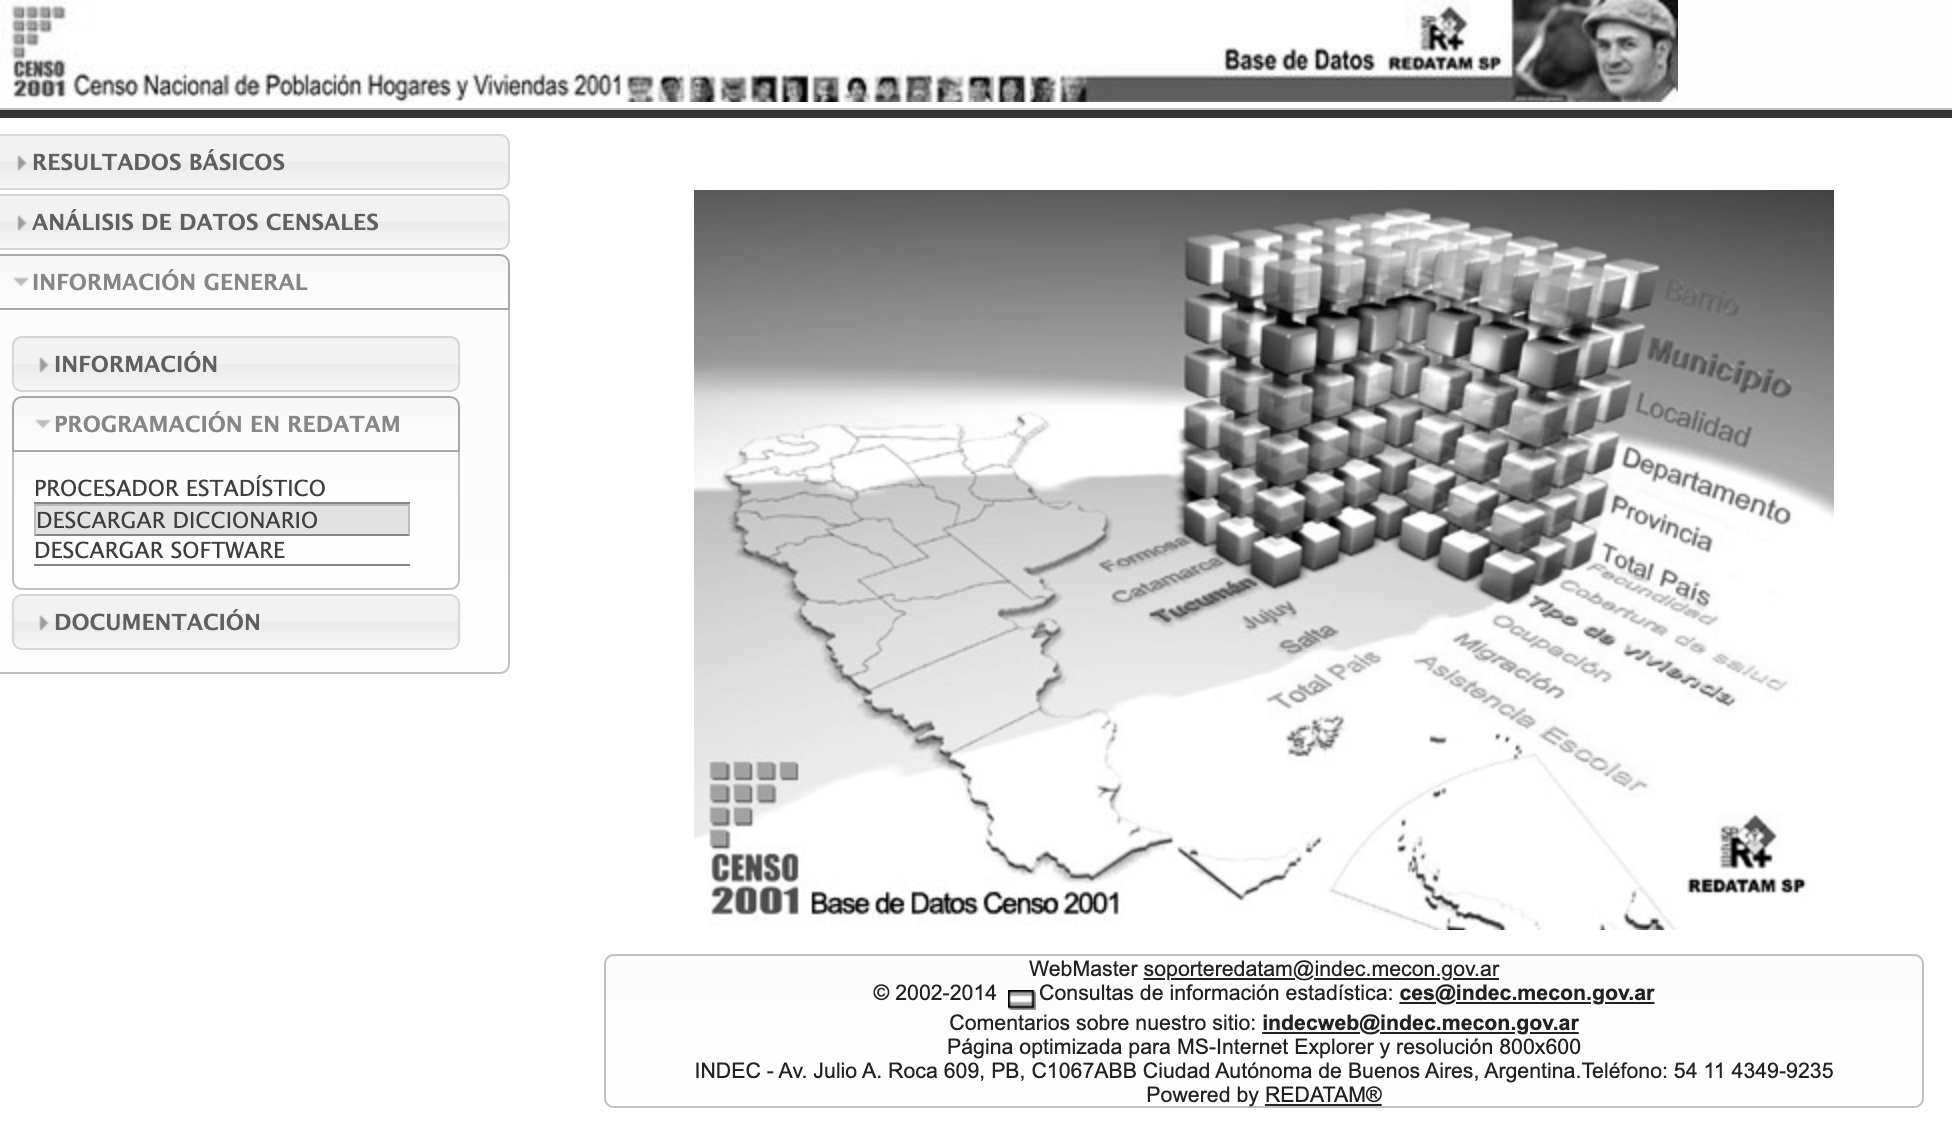
\includegraphics[width=0.8\linewidth]{imagenes/dic2001} 

}

\caption{Descargar diccionario}\label{fig:unnamed-chunk-34}
\end{figure}

\begin{figure}

{\centering 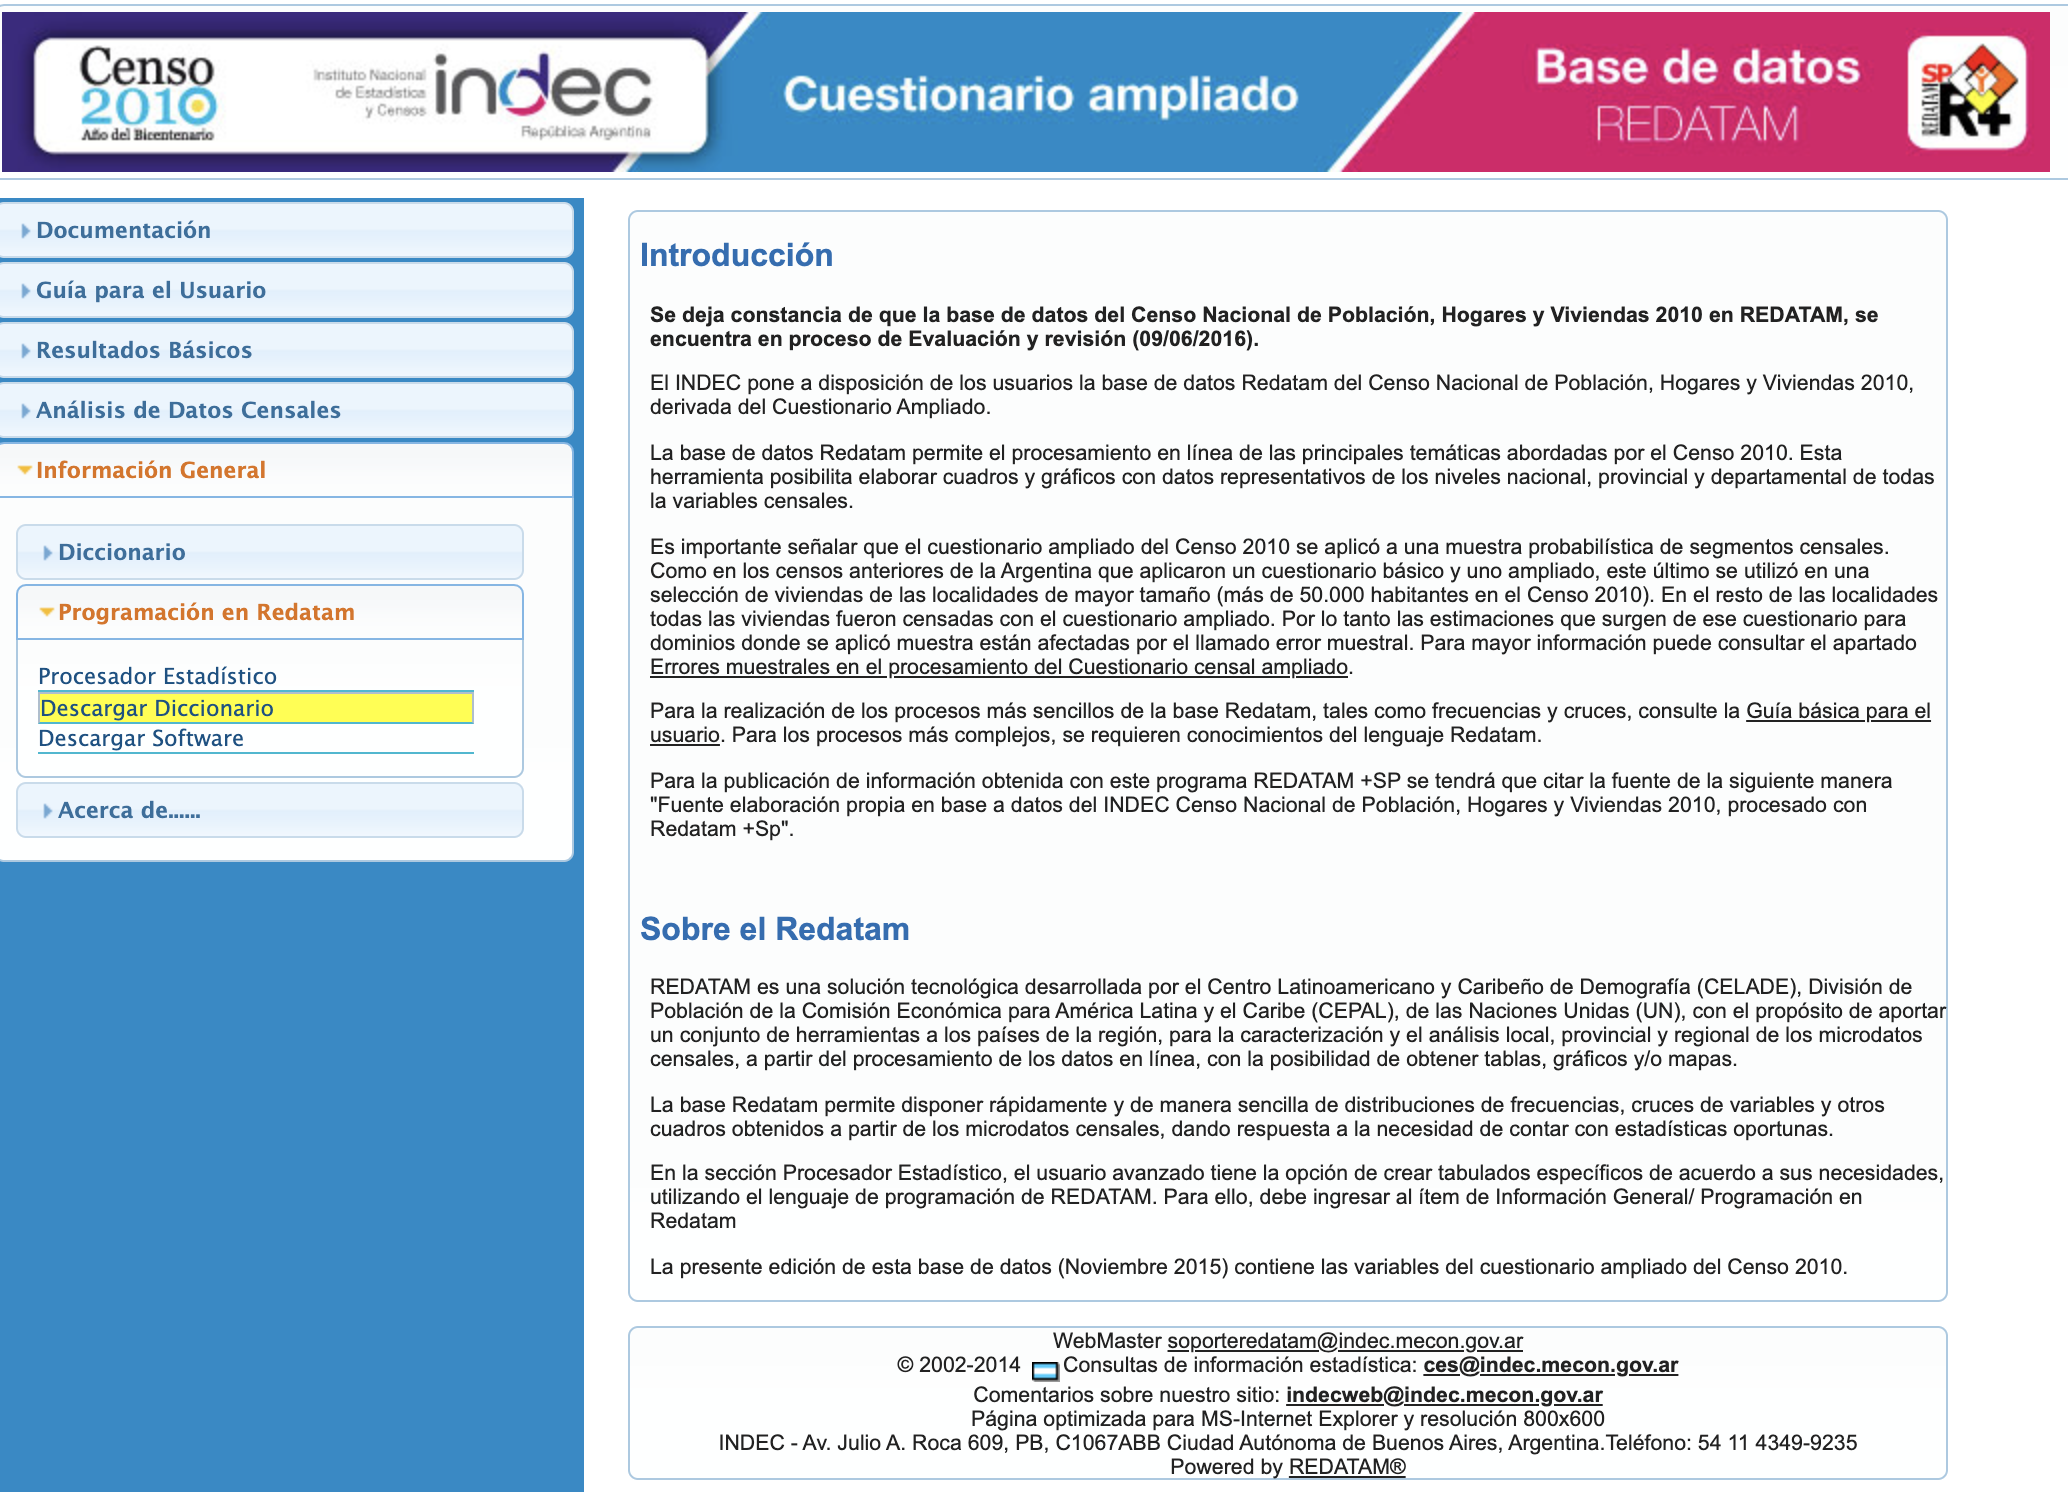
\includegraphics[width=0.8\linewidth]{imagenes/dic2010} 

}

\caption{Descargar diccionario2}\label{fig:unnamed-chunk-35}
\end{figure}

\hypertarget{transformaciuxf3n-del-diccionario-original}{%
\paragraph{Transformación del diccionario original}\label{transformaciuxf3n-del-diccionario-original}}

En base estas limitaciones del REDATAM, un investigador argentino, Pablo De Grande, desarrolló y liberó una herramienta de software para extraer la base completa (a nivel de personas, anonimizada) de cualquier censo hecho con REDATAM.

En su blog \href{https://idiscontinuos.wordpress.com/2015/03/21/convirtiendo-bases-redatam-a-spss/}{Discontinuos} se puede acceder al software \href{https://www.aacademica.org/conversor.redatam}{Converser Redatam} y explorar su modo de uso. Una vez bajados los diccionarios desde la web del INDEC, se pueden extraer los datos y guardarlos en un formato más adecuado para procesamientos estadísticos, por ejemplo, en ASCII.

\hypertarget{ipums-i}{%
\subsubsection{IPUMS-I}\label{ipums-i}}

Sólo cinco años después de la creación del CELADE, este organismo comenzó la Operación de Muestras de Censos (OMUECE), la más ambiciosa muestra internacional de censos del siglo XX. Gracias ello el archivo de microdatos censales de América Latina es uno los más completos de cualquier región del mundo (para más información ver artículos de McCaa y Jaspers-Faijer (2000) y McCaa, Esteve, Ruggles y Sobek (2004). Este proyecto fue el antecedente directo de las bases disponibles hoy en el IPUMS-I. Este espacio ofrece una colección, inventario, preservación de datos y documentación referida a muestras de censos en el mundo, con información armonizada, es decir, comparable entre países, de manera gratuita. Tiene una documentación bastante exhaustiva y facilita de esta forma la investigación comparativa. Una de las desventajas del proyecto IPUMS es que no posee mecanismos de validación con el INDEC y a veces resultan más confiables datos de los INDEC que IPUMS en algunas variables.

Para Argentina, contamos con microdatos de muestras censales sólo para los censos de 1970 a 2010.

Para les usuaries de \texttt{R} que quieran trabajar las bases con este programa, se recomienda que sigan las viñetas del paquete \href{https://cran.r-project.org/web/packages/ipumsr/vignettes/ipums.html}{\texttt{ipumsr}} para trabajar estos datos y la viñeta del \href{https://www.tidyverse.org/}{\texttt{tidyverse}} para su procesamiento.

\hypertarget{solicitud-directa-al-indec}{%
\subsubsection{Solicitud directa al INDEC}\label{solicitud-directa-al-indec}}

¿Qué se hace cuando las opciones de acceso a datos censales mencionadas previamente no satisfacen los requerimientos de información de los usuarios, ya sea porque se precisa información sobre un conjunto de variables específicas, o para un año censal en particular o para poder analizar los datos con mayores niveles de desagregación territorial? Pues bien, siempre está la opción de recurrir, con suerte variable, al INDEC.

Sabido es que el INDEC conserva ---de alguna manera y en algún sitio--- una copia de las bases de los censos realizados en el país. ¿Se puede acceder a las mismas? Si así fuera, ¿en qué formato y condiciones se podrían adquirir? ¿Cuál es el procedimiento a seguir para realizar esta solicitud? ¿Tiene algún costo? Lamentablemente no tenemos respuestas claras para estas preguntas pero es probable que existan posibilidades y criterios diferentes, porque es información que por razones que desconocemos, no se socializan.

En este sentido, resulta difícil de identificar los procedimientos vigentes en el INDEC. En algunos censos existieron en procedimientos claros y estandarizados para atender los pedidos de bases de datos censales, pero en otras no. Cuando esto último ocurre, suele suceder que los criterios varían en el tiempo y en función de las autoridades presentes en el organismo.

\hypertarget{otras-opciones-no-oficiales}{%
\subsubsection{Otras opciones no oficiales}\label{otras-opciones-no-oficiales}}

Como en casi todo en Argentina, hay también opciones no oficiales, que pueden ser útiles y traen serias preguntas y dudas acerca de la producción de estadísticas oficiales en la actualidad. Más de allá de los microdatos de los censos de 1869 y 1895, recuperados gracias al enorme trabajo de un \href{https://observatoriocensal.org/2015/12/01/recuperacion-de-microdatos-de-los-censos-argentinos-de-poblacion-1869-1895/}{usuario}, ha circulado recientemente una versión ``no oficial'' del Censo de 1991 en formato REDATAM. Esto se adelantó a la propia liberación de microdatos oficial, lo que nos lleva a preguntarnos cómo puede ser que el INDEC se quede por detrás a la demanda de los usuarios. Las estrategias de difusión y liberación de datos censales en Argentina han variado a lo largo de la historia, lo que denota la ausencia de un marco o criterio regulatorio común, así como las disimilitudes que existen en la concepción sobre los usos potenciales y resguardos requeridos con los datos. Si bien muy oportuno hoy en día, el acceso a los microdatos de censos históricos (digamos, previos al año 2000) no resulta una tarea sencilla. IPUMS-I ha facilitado enormemente esa tarea pero todavía queda mucho por hacer para que los usuarios tengan acceso a buenos datos censales.

\hypertarget{disponibilidad-en-detalle-para-el-estudio-de-clases-sociales}{%
\subsubsection{Disponibilidad en detalle para el estudio de clases sociales}\label{disponibilidad-en-detalle-para-el-estudio-de-clases-sociales}}

En definitiva y para ir cerrando este capítulo, para aquellos que utilizan datos censales y están interesados en el estudio de clases sociales durante el periodo 1960-2010, la disponibilidad de información se limita a: - Para 1960: tabulados publicados en papel. - Para 1970: tabulados publicados en papel y muestra de microdatos en IPUMS-I. - Para 1980: tabulados publicados en papel y muestra de microdatos en IPUMS-I. - Para 1991: tabulados publicados en papel, muestra de microdatos en IPUMS-I y una base no ``oficial'' sin información de metadatos. - Para 2001: tabulados publicados en papel, bases oficiales casi completas (diccionario) {[}no están todas las variables relevadas, en particular, la ocupación{]} y una base no ``oficial'' sin información de metadatos, con la variable ocupación incluida. - Para 2010: tabulados publicados en papel, bases oficiales completas (diccionarios) del cuestionario ampliado y básico.

\hypertarget{part-variables}{%
\part{Variables}\label{part-variables}}

\hypertarget{ocupacion}{%
\section{Las características económicas de la población}\label{ocupacion}}

En este capítulo se focaliza en las variables económicas que se investigaron, de manera no siempre uniforme, en las fuentes analizadas en los dos capítulos previos. Además se retoma el muy discutido tópico de los clasificadores de ocupación y su comparabilidad. Se presentan las distintas variables que son constitutivas para el estudio y la construcción de esquemas para la medición de las clases y la estratificación social, haciendo hincapié en limitaciones y los recaudos que deben considerarse en el uso de las mismas. Principalmente se revisa y analiza aquellas variables relevadas en los operativos del \textbf{INDEC}: censos y EPH.

Se exploran las siguientes preguntas:\\
- ¿Qué variables son necesarias considerar para estudiar empíricamente las clases sociales?\\
- ¿Cuáles son las limitaciones que se presentan en la utilización de dichas variables a la hora de trabajar con censos o encuestas de hogares?\\
- ¿Cómo fueron medidas las variables a lo largo del tiempo en el sistema estadístico argentino?\\
- ¿Cuáles son las ventajas y desventajas en el uso de las distintas clasificaciones (CNO, CIUO)?\\
- ¿Qué metodologías existen para armonizar los distintos clasificadores ocupacionales?

Al completar el capítulo se espera que los lectores puedan:

\begin{itemize}
\tightlist
\item
  Identificar las principales variables utilizadas en la construcción de esquemas de clases sociales.
\item
  Reconocer los distintos esquemas clasificatorios de la variable \textbf{ocupación}.
\item
  Reconocer las principales limitaciones que se presentan cuando se quieren hacer estudios de tipo longitudinales y se requiere la armonización de distintas clasificaciones que sufrieron cambios en el tiempo.
\end{itemize}

Para una mayor comprensión del capítulo se recomienda la lectura de las siguientes publicaciones:

\begin{itemize}
\item
  Chávez Molina, E., Bernasconi, F., \& Rodríguez de la Fuente, J. (\protect\hyperlink{ref-ChavezMolina.etal2020}{2020}). ``Propuesta de correspondencias entre CNO y CIUO. Sintaxis para SPSS, Stata y R. Herramientas Para La Investigación Social.'' Serie: Cuadernos de Métodos y Técnicas de La Investigación Social ¿Cómo Se Hace?, 6. \href{http://iigg.sociales.uba.ar/2020/09/30/his-6-propuesta-de-correspondencias-entre-cno-y-ciuo-sintaxis-para-spss-stata-y-r/?fbclid=IwAR3RvLDs7H8wYHDqUooZMEI74HIDS6MXT3YbEjstG44yt0DB9tFj0VwlT9A}{Link de descarga}
\item
  INDEC. (\protect\hyperlink{ref-INDEC2000a}{2000b}). Utilización de clasificadores de ocupación en las bases de datos de la encuesta permanente de hogares. \href{https://www.indec.gob.ar/dbindec/EPH_Clasif_Ocup_hasta_CNO_2001.doc}{Link de descarga}
\item
  INDEC. (\protect\hyperlink{ref-INDEC2018}{2018a}). Clasificador Nacional de Ocupaciones. Definiciones conceptuales. \href{https://www.indec.gob.ar/ftp/cuadros/menusuperior/clasificadores/definiciones_conceptuales_cno.pdf}{Link de descarga}
\item
  Sacco, N., \& Riveiro, M. (\protect\hyperlink{ref-Sacco2016b}{2016}). ``La Clasificación de Ocupaciones en el Sistema Estadístico Nacional''. \emph{Estudios Del Trabajo}, 51, 28. \href{https://aset.org.ar/ojs/revista/article/view/24}{Link de descarga}
\item
  INDEC. (\protect\hyperlink{ref-INDEC2018a}{2018b}). CNO. Clasificador Nacional de Ocupaciones. Versión 2017. \href{https://www.indec.gob.ar/ftp/cuadros/menusuperior/clasificadores/CNO_2017.pdf}{Link de descarga}
\item
  INDEC. (\protect\hyperlink{ref-INDEC2018b}{2018c}). CNO. Correspondencias entre el CNO-17 y la CIUO-08. \href{https://www.indec.gob.ar/ftp/cuadros/menusuperior/clasificadores/correspondencias_cno2017_ciuo2008.pdf}{Link de descarga}
\item
  OIT. (\protect\hyperlink{ref-OIT2008}{2008a}). Clasificación Internacional Uniforme de Ocupaciones (CIUO-08) -- Marco conceptual. OIT. \href{https://www.ilo.org/public/spanish/bureau/stat/isco/docs/annex1.pdf}{Link de descarga}
\item
  OIT. (\protect\hyperlink{ref-OIT2008a}{2008b}). Resolución sobre la actualización de la Clasificación Internacional Uniforme
  de Ocupaciones. OIT. \href{https://www.ilo.org/public/spanish/bureau/stat/isco/docs/resol08.pdf}{Link de descarga}
\item
  Torrado, S. (\protect\hyperlink{ref-Torrado1993a}{1993b}). El nuevo 'Clasificador Nacional de Ocupaciones del INDEC: Una fractura irreparable en el sistema estadístico nacional. \emph{Estudios del Trabajo}, 5, 85--120.
\end{itemize}

\hypertarget{consideraciones}{%
\subsection{Consideraciones previas}\label{consideraciones}}

\hypertarget{las-reglas-del-juego}{%
\subsubsection{Las reglas del juego}\label{las-reglas-del-juego}}

Si la idea es abordar la estructura socioeconómica, se debe tener en cuenta varias cuestiones antes de trabajar. En el \protect\hyperlink{estructura1}{Capítulo 2} se describieron distintas perspectivas teóricas sobre clases sociales que se han desarrollado tanto a nivel internacional como a nivel local en Argentina. Lo cierto es que se debe contar con una perspectiva que se adecúe a la pregunta de investigación y a objetivos. Luego, definir la metodología de estudio es crucial para poder organizar las técnicas de investigación que se implementarán. Partiendo de esta base, lo siguiente sería remitirse a las fuentes de datos a utilizar, según su accesibilidad y pertinencia. Una vez que se cuenta con los datos, se seleccionan las variables que sirvan para ``jugar'' con su caracterización. Se pueden elaborar sistemas de clases, construir nuevas variables, pensar en diferentes maneras de caracterizar a la estructura social y más. Todo ello con un mismo fin: analizar la sociedad a nivel macro.

En esta unidad se elabora una descripción de las variables económicas que se han investigado en las fuentes, prestando especial atención a las variables socio-ocupacionales porque han sido los principales insumos en el estudio de clases sociales, en especial, la ocupación. Se define su importancia, para qué ha servido en los estudios de Argentina, cómo tratarla y qué limitaciones se encuentran a la hora de implementarla. Además, presentamos otras variables que son de nuestro interés para construir esquemas de medición de clases sociales.

\hypertarget{la-estratificaciuxf3n-como-perspectiva-de-anuxe1lisis}{%
\subsubsection{La estratificación como perspectiva de análisis}\label{la-estratificaciuxf3n-como-perspectiva-de-anuxe1lisis}}

La estratificación es un proceso inherente a las sociedades modernas, que tiene que ver con la complejización de la actividad productiva. Las consecuencias de este fenómeno son relativas a la desigualdad de nuestras sociedades, lo cual ha despertado el interés de muchos cientistas sociales. Su estudio nos permite conocer los procesos de movilidad social inter e intra-generacionales y la configuración de la sociedad en grupos diferenciados. Lo cierto es que los recursos se distribuyen de manera desigual entre los miembros de nuestras sociedades, y esto genera distinciones entre ellos según la posición que ocupan.

Estudiar la estratificación implica seleccionar los indicadores y variables que contribuirán a la explicación sobre este proceso de diferenciación y diversificación social. Existe una larga tradición de tomar la educación, la ocupación y los ingresos como las tres principales patas de la investigación en estratificación (\protect\hyperlink{ref-Fujihara2020}{Fujihara, 2020}). La combinación de estas tres variables se conoce como estatus socio-económico (\protect\hyperlink{ref-Sno.Ganzeboom2017}{Sno \& Ganzeboom, 2017}). Al respecto, la ocupación ha tomado el papel principal peso, convirtiéndose en el ``mejor indicador'' (\protect\hyperlink{ref-Blau.Duncan1967}{Blau \& Duncan, 1967}) del estatus socio-económico.

En resumen, observar con los lentes de estratificación a la sociedad implica asumir que la diversificación de la actividad económica ha traído consigo la distinción en grupos según su tarea y posicionamiento en la sociedad, lo cual, a su vez, significa concebir una sociedad desigual, con mayor o menor apertura al ``movimiento'' de las personas dentro de este entramado de relaciones (ya sea ``hacia arriba'' o ``hacia abajo'') en el proceso de movilidad. Pero, ¿cómo medimos el proceso de estratificación?

\hypertarget{indicadores-de-la-estratificaciuxf3n-social}{%
\subsubsection{Indicadores de la estratificación social}\label{indicadores-de-la-estratificaciuxf3n-social}}

La investigación que aspira a comprender los cambios en la estructura social y su medición, se ha nutrido de dos grandes tipos de clasificación. Es decir que, a grandes rasgos, la investigación de la estructura social se ha bifurcado en estudios de clase o en estudios de estatus social. Si bien se parecen, no son lo mismo. Las clases sociales son categorías clasificatorias que se definen como variables discretas. Presentan a la sociedad como un conjunto de grupos que no necesariamente se encuentran ordenados de una manera particular. En cambio, el estatus social organiza a la sociedad según su carácter jerárquico. En este sentido, los grupos se diferencian por tener mayor o menor estatus con respecto a otros, es decir, en relación con los demás individuos. Esta aproximación está caracterizada por utilizar medidas continuas para ordenar a la sociedad. Las medidas empíricas de ordenamiento de la sociedad se diferencian en: escalas de prestigio ocupacional, índices de estatus socio-económico y sistemas de clases. Las primeras dos son medidas continuas mientras que la última consta de una clasificación en categorías discretas.

¿Por qué la ocupación es tan importante? Debemos entender la relevancia de la fuerza de trabajo para conocer sus implicancias en nuestras sociedades actuales.

\hypertarget{la-fuerza-de-trabajo-y-las-caracteruxedsticas-econuxf3micas-de-la-poblaciuxf3n}{%
\subsubsection{La fuerza de trabajo y las características económicas de la población}\label{la-fuerza-de-trabajo-y-las-caracteruxedsticas-econuxf3micas-de-la-poblaciuxf3n}}

La actividad económica es vital para cualquier sociedad. Cómo se organizan las personas alrededor de las actividades productivas y los procesos de estratificación asociados con la diferenciación social del trabajo son características fundamentales en nuestras sociedades. El estudio de la dinámica de la fuerza de trabajo es relevante para los científicos sociales en diversos aspectos: contribuye al debate sobre distintos temas de políticas públicas, y además puede responder preguntas fundamentales que interesan a los investigadores sobre estratificación.

La relación entre la población que contribuye a los procesos productivos en el mercado de trabajo y el resto, clasifica a las personas de acuerdo a su condición de actividad. La diferenciación entre los atributos de las personas económicamente activas de las inactivas permite el conocimiento de las características ocupacionales de los que participan en el mercado de trabajo. Para estudiar la actividad, los investigadores han desarrollado algunos conceptos como la Población Económicamente Activa (PEA) que aquí nos competen.

\hypertarget{las-variables-socio-ocupacionales}{%
\subsection{Las variables socio-ocupacionales}\label{las-variables-socio-ocupacionales}}

Las variables económicas de la población no han sido siempre las mismas, desde el censo de 1947 hasta el censo 2010, observándose una ampliación en la información recabada, según el número de variables a las que se hace referencia (\protect\hyperlink{ref-Sacco2015}{Sacco, 2015}). Como se vio en el \protect\hyperlink{fuentes2}{Capítulo 4}, si comparamos los censos a partir del de 1980 hasta el último, realizado en 2010, veremos cómo se ha diversificado la manera de medir la actividad económica en Argentina. Por su parte, las diferentes variables que ofrece la \textbf{EPH} (Tabla \ref{tab:vars1}) son similares a las del censo pero con algunas variaciones. Todas las variables aquí incluidas se encuentran disponibles en la base de Personas de la \textbf{EPH}.

\global\setlength{\Oldarrayrulewidth}{\arrayrulewidth}

\global\setlength{\Oldtabcolsep}{\tabcolsep}

\setlength{\tabcolsep}{0pt}

\renewcommand*{\arraystretch}{1.5}



\providecommand{\ascline}[3]{\noalign{\global\arrayrulewidth #1}\arrayrulecolor[HTML]{#2}\cline{#3}}

\begin{longtable}[c]{cccc}

\caption{Principales\ variables\ socio-ocupacionales\ de\ la\ EPH}\label{tab:vars1}\\

\ascline{1.5pt}{666666}{1-4}

\multicolumn{1}{>{}l}{\textcolor[HTML]{000000}{\fontsize{10}{10}\selectfont{\textbf{Variable}}}} & \multicolumn{1}{>{}l}{\textcolor[HTML]{000000}{\fontsize{10}{10}\selectfont{\textbf{Descripción}}}} & \multicolumn{1}{>{}l}{\textcolor[HTML]{000000}{\fontsize{10}{10}\selectfont{\textbf{Etiqueta}}}} & \multicolumn{1}{>{}l}{\textcolor[HTML]{000000}{\fontsize{10}{10}\selectfont{\textbf{Categorías}}}} \\

\ascline{1.5pt}{666666}{1-4}\endfirsthead \caption[]{Principales\ variables\ socio-ocupacionales\ de\ la\ EPH}\label{tab:vars1}\\

\ascline{1.5pt}{666666}{1-4}

\multicolumn{1}{>{}l}{\textcolor[HTML]{000000}{\fontsize{10}{10}\selectfont{\textbf{Variable}}}} & \multicolumn{1}{>{}l}{\textcolor[HTML]{000000}{\fontsize{10}{10}\selectfont{\textbf{Descripción}}}} & \multicolumn{1}{>{}l}{\textcolor[HTML]{000000}{\fontsize{10}{10}\selectfont{\textbf{Etiqueta}}}} & \multicolumn{1}{>{}l}{\textcolor[HTML]{000000}{\fontsize{10}{10}\selectfont{\textbf{Categorías}}}} \\

\ascline{1.5pt}{666666}{1-4}\endhead



\multicolumn{4}{>{}l}{\textcolor[HTML]{000000}{\fontsize{10}{10}\selectfont{Fuente:\ elaboración\ propia}}} \\

\endfoot



\multicolumn{1}{>{}l}{\textcolor[HTML]{000000}{\fontsize{10}{10}\selectfont{Condición\ de\ actividad}}} & \multicolumn{1}{>{}l}{\textcolor[HTML]{000000}{\fontsize{10}{10}\selectfont{Población\ activida\ o\ inactiva}}} & \multicolumn{1}{>{}l}{\textcolor[HTML]{000000}{\fontsize{10}{10}\selectfont{ESTADO}}} & \multicolumn{1}{>{}l}{\textcolor[HTML]{000000}{\fontsize{10}{10}\selectfont{Ocupado\ /\ Desocupado\ /\ Inactivo\ /\ Menor\ de\ 10\ años}}} \\





\multicolumn{1}{>{}l}{\textcolor[HTML]{000000}{\fontsize{10}{10}\selectfont{Categoría\ ocupacional}}} & \multicolumn{1}{>{}l}{\textcolor[HTML]{000000}{\fontsize{10}{10}\selectfont{Estatus\ jerárquico\ en\ el\ empleo}}} & \multicolumn{1}{>{}l}{\textcolor[HTML]{000000}{\fontsize{10}{10}\selectfont{CAT\_OCUP}}} & \multicolumn{1}{>{}l}{\textcolor[HTML]{000000}{\fontsize{10}{10}\selectfont{Patrón\ /\ Cuenta\ propia\ /\ Empleado\ /\ Trabajador\ familiar}}} \\





\multicolumn{1}{>{}l}{\textcolor[HTML]{000000}{\fontsize{10}{10}\selectfont{Ocupación}}} & \multicolumn{1}{>{}l}{\textcolor[HTML]{000000}{\fontsize{10}{10}\selectfont{Código\ de\ ocupación}}} & \multicolumn{1}{>{}l}{\textcolor[HTML]{000000}{\fontsize{10}{10}\selectfont{PP04D\_COD\ (ocupación\ actual)\ /\ PP11D\_COD\ (ocupación\ anterior)}}} & \multicolumn{1}{>{}l}{\textcolor[HTML]{000000}{\fontsize{10}{10}\selectfont{Ver\ Clasificador\ Nacional\ de\ Ocupaciones\ (CNO)}}} \\





\multicolumn{1}{>{}l}{\textcolor[HTML]{000000}{\fontsize{10}{10}\selectfont{Rama\ de\ actividad}}} & \multicolumn{1}{>{}l}{\textcolor[HTML]{000000}{\fontsize{10}{10}\selectfont{Sector\ industrial\ de\ la\ ocupación}}} & \multicolumn{1}{>{}l}{\textcolor[HTML]{000000}{\fontsize{10}{10}\selectfont{PP04B\_COD\ (ocupación\ actual)\ /\ PP11B\_COD\ (ocupación\ anterior)}}} & \multicolumn{1}{>{}l}{\textcolor[HTML]{000000}{\fontsize{10}{10}\selectfont{Ver\ Clasificador\ de\ Actividades\ Económicas\ para\ Encuestas\ Socio-demográficas\ del\ Mercosur\ (CAES\ -\ MERCOSUR)}}} \\





\multicolumn{1}{>{}l}{\textcolor[HTML]{000000}{\fontsize{10}{10}\selectfont{Tamaño\ del\ establecimiento}}} & \multicolumn{1}{>{}l}{\textcolor[HTML]{000000}{\fontsize{10}{10}\selectfont{Tamaño\ del\ establecimiento\ del\ trabajo}}} & \multicolumn{1}{>{}l}{\textcolor[HTML]{000000}{\fontsize{10}{10}\selectfont{PP04C\ /\ PP04c\_99}}} & \multicolumn{1}{>{}l}{\textcolor[HTML]{000000}{\fontsize{10}{10}\selectfont{Numérica}}} \\

\ascline{1.5pt}{666666}{1-4}



\end{longtable}



\arrayrulecolor[HTML]{000000}

\global\setlength{\arrayrulewidth}{\Oldarrayrulewidth}

\global\setlength{\tabcolsep}{\Oldtabcolsep}

\renewcommand*{\arraystretch}{1}

Ahora que sabemos cuál es la información que nuestras principales fuentes de datos contienen, describiremos de manera detallada cada una de ellas.

\hypertarget{condiciuxf3n-de-actividad}{%
\subsubsection{Condición de actividad}\label{condiciuxf3n-de-actividad}}

Las estadísticas de empleo distinguen dos grandes grupos de la población en edad laboral. El primero, es la población económicamente inactiva (\textbf{PNEA}), que incluye a todos aquellos que voluntariamente no trabajan o no trabajaban por pago o ganancia. El segundo es la población económicamente activa (\textbf{PEA}), que agrupa a aquellos que sí trabajan o trabajaban por pago o ganancia, como así también a aquellos que no tienen o tenían trabajo pero se encuentran o encontraban buscando activamente un empleo. Es decir, que en esta construcción los investigadores asumieron que la pérdida de empleo y la incapacidad de encontrar empleo representaba una falla en los mecanismos de asignación de los mercados de trabajo. En base a estos conceptos, los investigadores construyen las tasas de actividad, desempleo y empleo. El volumen, estructura y características de la \textbf{PEA}, en relación a sus características económicas, justifica su estudio para la demografía, la sociología y otras disciplinas.

La ONU define a la \textbf{condición de actividad} como aquello que ``permite distinguir entre personas económicamente activas y no económicamente activas. El estado de actividad es la relación actual o habitual de cada persona con la actividad económica durante un período determinado'' (\protect\hyperlink{ref-ONU1997}{ONU, 1997, p. 6}). Para estudiarla es necesario obtener datos de las personas con edad de trabajo, es decir, aquellos definidos como en edad laboral, que en Argentina es entre 15 y 65 años.

Si bien límite de edad suele no ser uniforme de acuerdo a la fuentes, esta variable comúnmente presenta las categorías de \emph{ocupado}, \emph{desocupado} e \emph{inactivo}, nos permite un primer recorte de nuestro objeto de estudio. Como veremos más adelante, desde la \textbf{condición de actividad} podremos diferenciar a la población ocupada, desocupada, activa o inactiva.

\hypertarget{ocupaciuxf3n}{%
\subsubsection{Ocupación}\label{ocupaciuxf3n}}

Para todas aquellas líneas de investigación que reconocen en la división del trabajo el núcleo de la desigualdad social, la clasificación de las ocupaciones constituye la columna vertebral de muchas, sino de la mayoría de las indagaciones sobre estratificación social (\protect\hyperlink{ref-Barozet2007}{Barozet, 2007}; \protect\hyperlink{ref-Crompton2008}{Crompton, 2008}). La \textbf{ocupación} compone un eje central de los estudios de mercados de trabajo y de la propia Sociología de las Ocupaciones. Su medición supone un conjunto de decisiones teóricas, metodológicas y operativas, que pocas veces tienen en los manuales la claridad y el espacio que merecen.

\hypertarget{la-clasificaciuxf3n-de-ocupaciones}{%
\paragraph[La Clasificación de Ocupaciones ]{\texorpdfstring{La Clasificación de Ocupaciones \footnote{Este texto está tomado parcialmente de Sacco \& Riveiro (\protect\hyperlink{ref-Sacco2016b}{2016})}}{La Clasificación de Ocupaciones }}\label{la-clasificaciuxf3n-de-ocupaciones}}

Los sistemas clasificatorios de ocupaciones son herramientas que permiten ubicar las ocupaciones de los y las encuestadas en grupos pre-definidos de acuerdo a las definiciones de cada clasificador. Los clasificadores de ocupación difieren no sólo con respecto del nivel de detalle y títulos ocupacionales específicos incluidos, sino también con respecto a su lógica. Por ejemplo, algunas clasificaciones distinguen estados de empleo dentro de las ocupaciones y otras no lo hacen. Algunas están fuertemente orientadas a distinguir situaciones en la industria y otras no. Algunos clasificadores se adaptan a las características particulares de los mercados de trabajo y otras reproducen estructuras ocupacionales de los países desarrollados. Estas diferencias reflejan, en cierta medida, la estructura ocupacional de las sociedades, pero también la historia e intenciones de las instituciones que las han desarrollado.

A nivel general, se pueden apreciar estas definiciones en las discusiones plasmadas en la actualización que lleva a la \textbf{Clasificación Internacional Uniforme de Ocupaciones} (CIUO) (\protect\hyperlink{ref-Budlender2003}{Budlender, 2003}; \protect\hyperlink{ref-Hoffmann1999}{Hoffmann, 1999}), o bien, a nivel local, las discusiones y producciones en torno al \textbf{Clasificador Nacional de Ocupaciones}, previas a su implantación (\protect\hyperlink{ref-Elizalde1987}{Elizalde, 1987}; \protect\hyperlink{ref-INDEC1990}{INDEC, 1990}, \protect\hyperlink{ref-INDEC1991}{1991}) y posteriores (\protect\hyperlink{ref-Elizalde1993}{Elizalde, 1993}; \protect\hyperlink{ref-Torrado1993}{Torrado, 1993a}, \protect\hyperlink{ref-Torrado1993a}{1993b}). Dada la complejidad intrínseca de la variable ocupación, así como de la exigencia explicativa que se le reclama, no es de extrañar que su medición y comparabilidad (a nivel transversal interno como a nivel regional e internacional) haya sido difícil de lograr. Diversas razones se dieron para esto.

Las clasificaciones de ocupación tienden a diferir tanto a nivel nacional como en el tiempo. Cada sistema estadístico nacional busca establecer una clasificación que capte de la mejor forma posible las particularidades de la estructura ocupacional de su país, que, por definición, no está exenta de cambios, especialmente desde el punto de vista del desarrollo tecnológico. En segundo lugar, existe una amplia disparidad entre la lógica y el contenido de los clasificadores de ocupación al aplicarse al análisis de datos concretos; esto en parte muestra las diferencias en los intereses teóricos por detrás de los sistemas clasificatorios, pero también es resultado de la falta de coordinación tanto de la investigación social como de los procesos estadísticos planificados a largo plazo por las instituciones gubernamentales (\protect\hyperlink{ref-Ganzeboom1996}{H. B. G. Ganzeboom \& Treiman, 1996}).

\hypertarget{la-clasificaciuxf3n-internacional-uniforme-de-ocupaciones-ciuo-de-la-oit}{%
\paragraph{La Clasificación Internacional Uniforme de Ocupaciones (CIUO) de la OIT}\label{la-clasificaciuxf3n-internacional-uniforme-de-ocupaciones-ciuo-de-la-oit}}

La \textbf{Organización Internacional del Trabajo} (OIT) de la ONU ha elaborado la \textbf{CIUO} por primera vez en 1958, con revisiones en 1968, 1988 y 2008 para tratar de solucionar estos problemas (\href{https://www.ilo.org/public/spanish/bureau/stat/isco/}{ver página web de la OIT}). Uno de los principales objetivos de la \textbf{CIUO} es proporcionar a los INES (institutos nacionales estadísticos) un punto de partida para organizar sus clasificaciones nacionales. Sin embargo, estas revisiones periódicas de la OIT hacen necesaria a su vez otras revisiones dentro cada uno de los INES.

La \textbf{Clasificación Internacional Uniforme de Ocupaciones} (\textbf{CIUO}) es una clasificación de la Organización Internacional del Trabajo. Es una herramienta para organizar los empleos en grupos, según las tareas de cada empleo.

Existen varias versiones de la \textbf{CIUO}. La primera es la \textbf{CIUO-58}, y data del año 1957. La segunda es la \textbf{CIUO-68}, que fue adoptada en 1966. La tercera versión, la \textbf{CIUO-88}, fue adoptada por la Decimocuarta Conferencia Internacional de Estadísticos del Trabajo en 1987. La cuarta y última es de diciembre del 2007 y se conoce como la \textbf{CIUO-08}. Los principios básicos y la estructura de la clasificación se mantuvieron pero se mejoraron algunas áreas.

La \textbf{CIUO-08} ofrece 436 grupos ocupacionales organizados en una jerarquía de cuatro dígito, comenzando por el nivel más agregado que trae como resultado a 10 grupos principales, seguidos de 43 sub-grupos principales, 130 grupos menores y todo el resto son grupos unitarios (\protect\hyperlink{ref-OIT}{OIT, n.d., p. 2012}). La versión más reciente de la CIUO ha incorporado algunos títulos ocupacionales que no estaban presente en las anteriores, por ejemplo, ``ayudantes de cocina''. La ventaja de esta estructura es que permite codificar ocupaciones con un nivel de detalle a cuatro dígitos, lo que significa que si buscamos mayor detalle, necesitaremos más cantidad de dígitos del código CIUO.

Los grupos principales a mayor nivel de agregación, es decir, a un dígito son:\\
0 Ocupaciones de las Fuerzas Armadas\\
1 Gerentes\\
2 Profesionales\\
3 Técnicos y Profesionales Asociados\\
4 Trabajadores de Apoyo Administrativo\\
5 Trabajadores de Servicios y Ventas\\
6 Trabajadores calificados agrícolas, forestales y pesqueros\\
7 Trabajadores artesanos y afines\\
8 Operadores y ensambladores de planta y maquinaria\\
9 Ocupaciones Elementales

La mayor información sobre las ocupaciones está incluida en los siguientes grupos. Tomando los grupos principales (``Gerentes'', con código 1000) se provee un ejemplo de un sub-grupo principal como es ``Jefes ejecutivos, altos funcionarios y legisladores (11)''; un grupo menor como ``Legisladores y Altos funcionarios (111)'' y en el nivel de mayor detalle, tenemos al grupo unitario de ``Oficiales de Alto Gobierno (1112)''. La estructura funciona como un set de cajas de diferente tamaño: las más pequeñas (grupos unitarios) están incluidas dentro de las más grandes y esto queda claro según el número de dígitos utilizado.

La característica por la cual se diferencian los grupos de la \textbf{CIUO-O8} es la calificación requerida para el trabajo. Por ejemplo, al diferenciar ``Profesionales (2)'' de ``Técnicos y Profesionales Asociados (3)''. Además, hay una separación entre quienes operan con máquinas y aquellos que no, en el caso de ``Trabajadores artesanos y afines (7)'' y ``Operadores y ensambladores de planta y máquinaria (8)''.

Si bien el mínimo común denominador de todas las clasificaciones son los títulos ocupacionales, la forma en la que se define la medición de la ocupación varía en cada clasificador, incluso desde la propia definición de ocupación. Por un lado, en la \textbf{CIUO-08}, ``se entiende por ocupación, un conjunto de empleos cuyas principales tareas y cometidos se caracterizan por un alto grado de similitud'', y define al empleo como un ``conjunto de tareas y cometidos desempeñados por una persona, o que se prevé que ésta desempeñe, para un empleador particular, incluido el empleo por cuenta propia'' (\protect\hyperlink{ref-OIT2008}{OIT, 2008a}). Se trata de una definición vinculada a la clasificación de grupos de tareas y responsabilidades muy similares.

Para facilitar comparaciones entre naciones, las recomendaciones internacionales sugieren utilizar la clasificación de ocupaciones de acuerdo a normas de clasificación nacionales que puedan establecer su homologación con la última revisión de la \textbf{CIUO} mediante una doble codificación o mediante una correspondencia de los grupos detallados de la clasificación nacional con los de la clasificación de la OIT. Adicionalmente, especifican que los países deberían codificar los datos ocupacionales que hayan reunido al nivel más bajo posible que apoye la información recibida. Para facilitar una codificación detallada y exacta, sería útil que en el cuestionario se preguntara el título ocupacional de cada persona activa y se pidiera una breve descripción de las tareas y funciones realizadas en el empleo (\protect\hyperlink{ref-ONUOIT2010}{ONU-OIT, 2010, pp. 179--180}).

\hypertarget{clasificador-nacional-de-ocupaciones-cno-del-indec-argentina}{%
\paragraph{Clasificador Nacional de Ocupaciones (CNO) del INDEC Argentina}\label{clasificador-nacional-de-ocupaciones-cno-del-indec-argentina}}

El \textbf{CNO (Clasificador Nacional de Ocupaciones)} es un sistema de clasificación de ocupaciones. Podemos definirlo como una herramienta que agrupa diferentes ocupaciones de acuerdo a un criterio preestablecido (\protect\hyperlink{ref-ChavezMolina.etal2020}{Chávez Molina et al., 2020}).

El \textbf{CNO-01} (definido actualmente como CNO-17) define a las ocupaciones, que son la ``unidad de análisis'' del clasificador, como la ``forma concreta de la división singular del trabajo y de su sistema de relaciones dentro de las unidades productivas'' y como ``los procesos de trabajo parciales o individuales existentes en ellas'' (\protect\hyperlink{ref-INDEC2005}{INDEC, 2005, p. 16}). Esta definición de ocupación se distingue de la que provee la \textbf{CIUO}, siendo que ambas poseen marcos conceptuales diferentes, pero un mismo objetivo, clasificar ocupaciones.

La estructura del \textbf{CNO-17} se compone de 5 dígitos, que contienen 4 dimensiones de análisis:

\emph{1° y 2° dígito: Carácter Ocupacional\\
}3° dígito: Jerarquía Ocupacional\\
\emph{4° dígito: Tecnología Ocupacional\\
}5° dígito: Calificación Ocupacional Carácter

\hypertarget{caruxe1cter-ocupacional}{%
\subparagraph{Carácter Ocupacional}\label{caruxe1cter-ocupacional}}

Clasifica la ocupación en base al producto que se genera en el proceso de trabajo, más allá de la rama de actividad del establecimiento donde se realice la actividad laboral.

El primer dígito señala los 10 grandes grupos ocupacionales que van del 0 al 9. Esos grupos luego se desagregan con un segundo dígito en otros subgrupos de carácter más específico.

A continuación, presentamos los 10 grandes grupos ocupacionales de mayor nivel de agregación, es decir a un dígito de codificación. Además, mostramos un ejemplo de la clasificación a dos dígitos, dentro del primer grupo ``Ocupaciones de dirección''.

0 Ocupaciones de dirección.\\
00 Funcionarios del poder ejecutivo nacional, provincial, municipal y/o departamental.\\
01 Funcionarios del poder legislativo nacional, provincial, municipal y/o departamental.\\
02 Funcionarios del poder judicial, federal, nacional, provincial, municipal y/o departamental.\\
03 Directivos de organismos, empresas e instituciones estatales.\\
04 Directivos de instituciones sociales.\\
05 Directivos de pequeñas y microempresas.\\
06 Directivos de medianas empresas privadas productoras de bienes y servicios.\\
07 Directivos de grandes empresas privadas productoras de bienes y servicios.

1 Ocupaciones de gestión administrativa, de planificación, de control de gestión y jurídico-legal.

2 Ocupaciones de gestión presupuestaria, contable y financiera.

3 Ocupaciones de comercialización, de transporte, de almacenaje y de telecomunicaciones.

4 Ocupaciones de servicios sociales básicos.

5 Ocupaciones de servicios varios.

6 Ocupaciones agropecuarias, forestales, de la pesca y de la caza.

7 Ocupaciones de la producción extractiva, energética, de construcción e infraestructura.

8 Ocupaciones de la producción artesanal, industrial y de reparación de bienes de consumo.

9 Ocupaciones auxiliares de la producción de bienes y de la prestación de servicios.

\hypertarget{jerarquuxeda-ocupacional}{%
\subparagraph{Jerarquía Ocupacional}\label{jerarquuxeda-ocupacional}}

Clasifica la ocupación según la jerarquía que ocupa en la organización del proceso de trabajo. Reconoce cuatro categorías que se traducen en los siguientes valores:

\begin{enumerate}
\def\labelenumi{\arabic{enumi}.}
\setcounter{enumi}{-1}
\tightlist
\item
  Dirección\\
\item
  Cuenta propia\\
\item
  Jefes\\
\item
  Trabajadores asalariados Tecnología
\end{enumerate}

\hypertarget{tecnologuxeda-ocupacional}{%
\subparagraph{Tecnología Ocupacional}\label{tecnologuxeda-ocupacional}}

La tecnología ocupacional clasifica la ocupación de acuerdo al tipo de tecnología utilizada en el proceso de trabajo específico. Las categorías y valores para esta dimensión son las siguientes:

\begin{enumerate}
\def\labelenumi{\arabic{enumi}.}
\tightlist
\item
  Sin operación de máquina\\
\item
  Operación de maquinaria y equipos electromecánicos\\
\item
  Operación de sistemas y equipos informatizados
\end{enumerate}

Debe realizarse la siguiente aclaración: en el caso de los directores, jefes y patrones, el valor siempre es 0 (cero). La dimensión de la tecnología ocupacional no es contemplada para estos casos por una cuestión de comparabilidad con el CNO-91.

\hypertarget{calificaciuxf3n-ocupacional}{%
\subparagraph{Calificación Ocupacional}\label{calificaciuxf3n-ocupacional}}

Clasifica la ocupación según la complejidad del proceso de trabajo específico, considerando los conocimientos y las competencias necesarias para su ejecución. Las categorías y valores para esta dimensión son:

\begin{enumerate}
\def\labelenumi{\arabic{enumi}.}
\tightlist
\item
  Profesionales\\
\item
  Técnicos\\
\item
  Operativo\\
\item
  No calificado
\end{enumerate}

Es importante realizar la distinción entre calificación de la ocupación y calificación requerida para la ocupación. La primera es la calificación del proceso de trabajo que involucra a dicha ocupación y la segunda es el nivel de formación necesario para acceder a cierta ocupación. En este caso, el 5º dígito del \textbf{CNO-17} hace referencia a la primera de las acepciones.

Ilustramos, con un ejemplo ---Tabla \ref{tab:cnotabla}---, la clasificación en su mayor nivel de desagregación, a 5 dígitos, mostrando en el siguiente cuadro realizado por Chávez Molina et al. (\protect\hyperlink{ref-ChavezMolina.etal2020}{2020}) el código ocupacional de los ``Jefes de la producción industrial y artesanal con calificación profesional (80201)''.

\global\setlength{\Oldarrayrulewidth}{\arrayrulewidth}

\global\setlength{\Oldtabcolsep}{\tabcolsep}

\setlength{\tabcolsep}{0pt}

\renewcommand*{\arraystretch}{1.5}



\providecommand{\ascline}[3]{\noalign{\global\arrayrulewidth #1}\arrayrulecolor[HTML]{#2}\cline{#3}}

\begin{longtable}[c]{cccc}

\caption{CNO\ 80.2.0.1:\ Jefes\ de\ la\ producción\ industrial\ y\ artesanal\ con\ calificación\ profesional}\label{tab:cnotabla}\\

\ascline{1.5pt}{666666}{1-4}

\multicolumn{1}{>{}l}{\textcolor[HTML]{000000}{\fontsize{10}{10}\selectfont{\textbf{Dígitos}}}} & \multicolumn{1}{>{}l}{\textcolor[HTML]{000000}{\fontsize{10}{10}\selectfont{\textbf{Dimensión}}}} & \multicolumn{1}{>{}l}{\textcolor[HTML]{000000}{\fontsize{10}{10}\selectfont{\textbf{Dígitos\ CNO}}}} & \multicolumn{1}{>{}l}{\textcolor[HTML]{000000}{\fontsize{10}{10}\selectfont{\textbf{Detalle\ dígitos}}}} \\

\ascline{1.5pt}{666666}{1-4}\endfirsthead \caption[]{CNO\ 80.2.0.1:\ Jefes\ de\ la\ producción\ industrial\ y\ artesanal\ con\ calificación\ profesional}\label{tab:cnotabla}\\

\ascline{1.5pt}{666666}{1-4}

\multicolumn{1}{>{}l}{\textcolor[HTML]{000000}{\fontsize{10}{10}\selectfont{\textbf{Dígitos}}}} & \multicolumn{1}{>{}l}{\textcolor[HTML]{000000}{\fontsize{10}{10}\selectfont{\textbf{Dimensión}}}} & \multicolumn{1}{>{}l}{\textcolor[HTML]{000000}{\fontsize{10}{10}\selectfont{\textbf{Dígitos\ CNO}}}} & \multicolumn{1}{>{}l}{\textcolor[HTML]{000000}{\fontsize{10}{10}\selectfont{\textbf{Detalle\ dígitos}}}} \\

\ascline{1.5pt}{666666}{1-4}\endhead



\multicolumn{4}{>{}l}{\textcolor[HTML]{000000}{\fontsize{10}{10}\selectfont{Fuente:\ Chávez\ Molina\ et\ al.\ (2020)}}} \\

\endfoot



\multicolumn{1}{>{}l}{\textcolor[HTML]{000000}{\fontsize{10}{10}\selectfont{1°\ y\ 2°}}} & \multicolumn{1}{>{}l}{\textcolor[HTML]{000000}{\fontsize{10}{10}\selectfont{Carácter}}} & \multicolumn{1}{>{}l}{\textcolor[HTML]{000000}{\fontsize{10}{10}\selectfont{80}}} & \multicolumn{1}{>{}l}{\textcolor[HTML]{000000}{\fontsize{10}{10}\selectfont{Ocupaciones\ de\ la\ producción\ industrial\ y\ artesanal}}} \\





\multicolumn{1}{>{}l}{\textcolor[HTML]{000000}{\fontsize{10}{10}\selectfont{3°}}} & \multicolumn{1}{>{}l}{\textcolor[HTML]{000000}{\fontsize{10}{10}\selectfont{Jerarquía}}} & \multicolumn{1}{>{}l}{\textcolor[HTML]{000000}{\fontsize{10}{10}\selectfont{2}}} & \multicolumn{1}{>{}l}{\textcolor[HTML]{000000}{\fontsize{10}{10}\selectfont{Jefes}}} \\





\multicolumn{1}{>{}l}{\textcolor[HTML]{000000}{\fontsize{10}{10}\selectfont{4°}}} & \multicolumn{1}{>{}l}{\textcolor[HTML]{000000}{\fontsize{10}{10}\selectfont{Tecnología}}} & \multicolumn{1}{>{}l}{\textcolor[HTML]{000000}{\fontsize{10}{10}\selectfont{0}}} & \multicolumn{1}{>{}l}{\textcolor[HTML]{000000}{\fontsize{10}{10}\selectfont{No\ corresponde}}} \\





\multicolumn{1}{>{}l}{\textcolor[HTML]{000000}{\fontsize{10}{10}\selectfont{5°}}} & \multicolumn{1}{>{}l}{\textcolor[HTML]{000000}{\fontsize{10}{10}\selectfont{Calificación}}} & \multicolumn{1}{>{}l}{\textcolor[HTML]{000000}{\fontsize{10}{10}\selectfont{1}}} & \multicolumn{1}{>{}l}{\textcolor[HTML]{000000}{\fontsize{10}{10}\selectfont{Profesionales}}} \\

\ascline{1.5pt}{666666}{1-4}



\end{longtable}



\arrayrulecolor[HTML]{000000}

\global\setlength{\arrayrulewidth}{\Oldarrayrulewidth}

\global\setlength{\tabcolsep}{\Oldtabcolsep}

\renewcommand*{\arraystretch}{1}

Dentro del grupo \texttt{80201} se encuentran ocupaciones tales como ``Jefe de planta industrial'' y ``Jefe de laboratorio''. El primer dígito, señala al grupo 8, que define tareas vinculadas a la producción de bienes, ya sea industrial o artesanal. Incluyendo un mayor nivel de detalle a dos dígitos, el grupo 80, alude a ocupaciones relativas a la transformación de materias primas para la elaboración de bienes industriales o artesanales, tanto bienes finales como intermedios. El 3º dígito permite establecer que la ocupación se inserta en una posición de jefatura. Al 4º código de la tecnología siempre se le adjudica el valor de 0 en los casos de patrones, directores y jefes. Por último, el 5º dígito describe que esta ocupación presenta una calificación profesional.

\hypertarget{compatibilidad-entre-la-cno-y-la-ciuo}{%
\paragraph{Compatibilidad entre la CNO y la CIUO}\label{compatibilidad-entre-la-cno-y-la-ciuo}}

Distinguiendo los censos modernos de población en Argentina -de 1960 a 2010-, el código ocupacional empleado en el censo de 1960 era compatible a nivel de 4 dígitos con la \textbf{CIUO} en su versión de 1958 mientras que en el censo de 1970 se utilizó la \textbf{CIUO-1968} a nivel de 3 dígitos. En el censo de 1980 la variable ocupación fue codificada por el Código Ocupacional (CO) que permitía homologar sus códigos a nivel de 1 o 2 dígitos en algunas ocupaciones con la \textbf{CIUO-68}.

En parte gracias a debates llevados a cabo durante el periodo intercensal 1980-1991, se propusieron procedimientos clasificatorios alternativos de codificación de esta variable en los censos de población llevados a cabo por el \textbf{INDEC}. Siguiendo las recomendaciones internacionales que sugerían a los institutos de estadística construir sus propios clasificadores para adaptarlos a las particularidades de los mercados de trabajo en cada país, el \textbf{CNO} fue elaborado por el \textbf{INDEC} actualizando el CO de la \textbf{EPH}, cuyas distintas versiones previas (con mayores niveles de agregación) fueron utilizadas desde la aplicación de la encuesta, a principios de la década del setenta. De esta forma, desde el censo de 1991 se aplicó el \textbf{CNO} sucesivamente en los censo del 2001 y 2010, en distintas versiones y a distintos niveles de apertura.

Esta estabilidad del clasificador ha posibilitado el desarrollo de una serie de investigaciones desde el \textbf{INDEC}, por ejemplo, los documentos de la Serie Estructura Ocupacional del Programa de Medición y Análisis de la Estructura Ocupacional, y su utilización en investigaciones académicas, realizadas con información proveniente de la \textbf{EPH} y la Encuesta Anual de Hogares Urbanos. Sin embargo, el clasificador no ha pasado a ser parte un insumo habitual para la generación de datos ocupacionales primarios por fuera del \textbf{INDEC}, limitando así su aceptación por fuera del Sistema Estadístico Nacional (SEN).

Con el \textbf{CNO} se contó por primera vez en la historia del SEN con el mismo sistema clasificatorio de las ocupaciones en tres relevamientos censales sucesivos y en la \textbf{EPH}. En las primeras versiones del \textbf{CNO} (o CO-EPH), su máxima apertura permitía un empalme con la \textbf{CIUO} a 2 dígitos, cuya homogeneización, si bien no perfecta, era razonablemente directa (\protect\hyperlink{ref-INDEC2000}{INDEC, 2000a}). Una vez actualizando el sistema clasificatorio, la versión a 3 dígitos aplicada tanto en la encuesta como en el censo de 1991, los empalmes entre la \textbf{CIUO} se volvieron irrealizables más allá del segundo dígito (\protect\hyperlink{ref-INDEC1998}{INDEC, 1998}). Esto implicó niveles de comparabilidad con la \textbf{CIUO} limitados a mayor grado de des-agregación de la información.

El \textbf{CNO-91} empleó 3 dígitos para la codificación de ocupaciones, mientras que en el 2001 se utilizó una versión a 5 dígitos. Por su parte, la información recabada por el censo de 2010 sólo computó el nombre de la ocupación, sin preguntar por la tarea, lo que supuso codificar sólo al nivel de 1 dígito (carácter) del \textbf{CNO}, produciendo una ruptura de la serie comenzada en 1991 a mayores niveles de des-agregación.

No sólo se observó un cambio en la cantidad de dígitos de cada codificador aplicado, sino también en la información que cada uno otorga. Por ejemplo, si bien en el censo de 1980 sólo se codificó a un dígito, la propia estructura y lógica de la \textbf{CIUO} permite comparaciones con otros codificadores (dado que es un sistema clasificatorio muy dependiente de la calificación) mientras que en el 2010 el nivel de agregación no dice mucho más que una denominación, sin poder realizar diferenciación social interna alguna de cada una de ellas, tales como las que provee la calificación de las tareas.

\hypertarget{debates-de-clasificaciuxf3n}{%
\subparagraph{Debates de clasificación}\label{debates-de-clasificaciuxf3n}}

Las modificaciones a nivel interno con el clasificador del censo de 1980 dieron lugar a encendidos debates sobre la conveniencia de modificar o no las nomenclaturas estadísticas. Uno de los argumentos de Torrado (\protect\hyperlink{ref-Torrado1993a}{1993b}) fue que con el \textbf{CNO-91} (aplicado para el censo de 1991) las tareas que relevó el censo no fueron codificadas, perdiéndose de esta forma el dato sobre la ocupación y las tareas. El contra-argumento del equipo encargado de elaborar el \textbf{CNO-91} (\protect\hyperlink{ref-Elizalde1993}{Elizalde, 1993}) era que ningún sistema clasificatorio admitía contar con el dato sobre la ocupación recogido por el censo, sino que todos permiten reemplazarlo por la denominación del subgrupo al nivel menor de agregación en el que es clasificada.

Torrado (\protect\hyperlink{ref-Torrado1993a}{1993b}) también objetaba que la aplicación del \textbf{CNO-91} producía una ruptura de comparabilidad con los nomencladores nacionales precedentes y con los nomencladores internacionales. A su vez, que el \textbf{CNO-91} requería para su codificación de información adicional a la ocupación mientras que la \textbf{CIUO} sólo requería la respuesta a la pregunta sobre ``Ocupación principal'' para poder asignar una ocupación individual a un grupo dado del nomenclador (es decir, el criterio organizador de la clasificación era unidimensional). El \textbf{CNO-91}, por el contrario, para la definición de sus categorías se requería información sobre variables económicas adicionales a la ocupación (tales como categoría ocupacional, rama de actividad, tamaño del establecimiento de los patrones). Esto implicó que la aplicación del \textbf{CNO}, en rigor, sólo fuera posible en el caso de fuentes que investiguen todas las variables adicionales a la ocupación (prácticamente, ninguna salvo la \textbf{EPH}). Significó además que en la utilización del \textbf{CNO} se introdujera complicaciones en las tareas de codificación en el censo, ya de por sí complejas con los nomencladores anteriores.

Torrado (\protect\hyperlink{ref-Torrado1993a}{1993b}) sostenía que la aplicación de este sistema clasificatorio traería consigo un aumento considerable tanto de los costos de procesamiento del censo como de los inevitables errores de codificación y falta de oportunidad de las publicaciones de estos datos. Lo sucedido \textbf{a posteriori} en el censo de 1991 y el de 2001 no hizo más que confirmar algunas de estas advertencias. En efecto, tanto en el censo de 1991 como en el censo de 2001, los tabulados y bases de datos publicados con esta información fueron de poco detalle (salvo en bases de datos no oficiales) y divulgadas relativamente con poca oportunidad y, por ende, de dudosa calidad, a pesar de que, por ejemplo, en la medición y clasificación de las ocupaciones en el censo de 2001, se utilizó, por primera vez, un sistema informático que permitió la codificación automática de más del 55\% de las declaraciones sobre ocupación y en el que se codificaron el total de las declaraciones sobre esta variable relevadas por el censo. De hecho, ante la falta de recursos humanos, en el censo de 1991 las tareas de codificación de las ocupaciones fueron muestreadas.

Esto parece (a falta de publicaciones oficiales) no haber sucedido en el censo de 2010. Si bien el clasificador utilizado tanto en el censo 2001 como en el 2010 es el mismo, no fueron iguales las decisiones en lo que refiere al tratamiento y difusión de los datos. El nivel de apertura de las ocupaciones en el censo 2010 no es informativo acerca de las tareas, ya que el nombre de la ocupación sólo muestra el carácter ocupacional, vinculado con el objeto o servicio que produce el proceso de trabajo del que forma parte la ocupación clasificada. A pesar de que esta decisión política y técnica no guarde relación directa con el \textbf{CNO} como instrumento, conlleva implicancias indirectas particulares: otros sistemas clasificatorios a nivel de un dígito, por ejemplo la \textbf{CIUO}, si bien en escaso grado de detalle, remiten, en su nivel más agregado, tanto las tareas como a la calificación ocupacional. Adicionalmente, los censos de 1991 y 2001 mostraron distintos tipos de límites a la captación de la condición de actividad, por ende, afectando a todas las variables relativas a las características económicas de población.

La aplicación del \textbf{CNO} en el censo de 1991 introdujo no sólo un cambio en el sistema clasificatorio con respecto al utilizado sobre todo en 1980 (también en 1960 y 1970), sino que hubo variaciones en su definición, la forma de medición, el diseño de la cédula, la lectura y procesamiento posterior de la información. A diferencia del censo de 2001, el censo de 1980 y el censo de 1991 preguntaron directamente por la tarea y ocupación. En el 2001, en cambio, se dividió la pregunta en dos: por un lado, se indagó el nombre de la ocupación, y, por el otro, la tarea.

\hypertarget{muxe9todos-de-correspondencia-entre-el-cno-y-la-ciuo}{%
\subparagraph{Métodos de correspondencia entre el CNO y la CIUO}\label{muxe9todos-de-correspondencia-entre-el-cno-y-la-ciuo}}

En los casos en los que se necesita realizar comparaciones entre información encontrada en distintas encuestas nacionales o con relevamientos internacionales, es necesario trabajar con un esquema clasificatorio de la ocupación que sea común. En este sentido, internacionalmente, la \textbf{CIUO} (en sus distintas versiones) funciona como ``lenguaje común'' en términos de la medición ocupacional. Una de las recomendaciones de la \textbf{OIT}, además de la construcción de instrumentos de medición ocupacional propios para cada situación nacional, es la elaboración de equivalencias entre el clasificador nacional y la \textbf{CIUO}.

De este modo a partir de la información brindada por \textbf{INDEC} (\protect\hyperlink{ref-ChavezMolina.etal2020}{Chávez Molina et al., 2020}; \protect\hyperlink{ref-INDEC2018b}{INDEC, 2018c}) es posible realizar esta conversión a nivel de dos dígitos de la \textbf{CIUO}. Siguiendo la metodología propuesta por el organismo estadístico, la mayor parte de los códigos del CNO presentan su equivalencia a dos dígitos de la \textbf{CIUO}, mientras que para algunos códigos específicos es necesario recurrir a la variable \textbf{rama de actividad} para poder hallar la correspondencia.

Para una propuesta mejorada de la metodología de \textbf{INDEC}, junto con las sintaxis para \texttt{SPSS}, \texttt{R} y \texttt{STATA}, puede consultarse Chávez Molina et al. (\protect\hyperlink{ref-ChavezMolina.etal2020}{2020}).

\hypertarget{rama-de-actividad}{%
\subsubsection{Rama de Actividad}\label{rama-de-actividad}}

La \textbf{Rama de Actividad} describe al sector industrial al que pertenece el establecimiento dentro del cual la persona ejerce o ejerció su empleo. Es decir, la unidad productiva en la cual las personas trabajan. A diferencia de otras variables económicas o socio-ocupacionales, la \textbf{rama de actividad} permite realizar diferenciaciones horizontales, no jerárquicas, a partir de la inserción de los trabajadores en las unidades productivas.

Tanto en la \textbf{EPH} como en el censo, se ha utilizado la codificación disponible según la ``Clasificación Industrial Internacional Uniforme de Actividades Económicas'' (\textbf{CIIU}) de las Naciones Unidas (\protect\hyperlink{ref-ONU2009a}{2009}). Para 1991, 2001 y 2010 esta variable no presenta modificaciones sustanciales por lo que, en términos generales, los datos disponibles, son comparables.

En el censo de 1980, fue codificada según la ``Clasificación Industrial Internacional Uniforme de Actividades Económicas'' (\textbf{CIIU}) de las Naciones Unidas (Revisión 2-1968), hasta el nivel de ramas específicas (dos dígitos). Para 1991 y 2001 esta variable no presentó modificaciones sustanciales. Más información puede encontrarse en este \href{https://www.indec.gob.ar/micro_sitios/clanae/default.asp}{link}.

En la \textbf{EPH} entre 1974, su primera onda, hasta 1980 inclusive, se han utilizado los tres primeros dígitos de la \textbf{CIIU}, Revisión 2, aunque la codificación original consta de hasta 5 dígitos a su nivel más detallado. A partir del año 1997, se ha utilizado la ``Clasificación Nacional de Actividades Económicas'' (ClaNAE-97) con un detalle a cinco dígitos. Más tarde, desde 2011, la \textbf{EPH} distingue las ramas de actividad según la ``Clasificación de Actividades Económicas para Encuestas Sociodemográficas del Mercosur'' (\textbf{CAES Mercosur 1.0}), utilizando los 5 dígitos del código. Así mismo, esta última versión del CAES es totalmente compatible con el \textbf{CIIU} en su revisión 4. En la Tabla \ref{tab:caes10} se observa un ejemplo de la CAES:

\global\setlength{\Oldarrayrulewidth}{\arrayrulewidth}

\global\setlength{\Oldtabcolsep}{\tabcolsep}

\setlength{\tabcolsep}{0pt}

\renewcommand*{\arraystretch}{1.5}



\providecommand{\ascline}[3]{\noalign{\global\arrayrulewidth #1}\arrayrulecolor[HTML]{#2}\cline{#3}}

\begin{longtable}[c]{ccc}

\caption{Ejemplo\ clasificación\ de\ Actividades\ Profesionales,\ Científicas\ y\ Técnicas\ -\ CAES\ 1.0}\label{tab:caes10}\\

\ascline{1.5pt}{666666}{1-3}

\multicolumn{1}{>{}l}{\textcolor[HTML]{000000}{\fontsize{10}{10}\selectfont{\textbf{Código}}}} & \multicolumn{1}{>{}l}{\textcolor[HTML]{000000}{\fontsize{10}{10}\selectfont{\textbf{Descripción}}}} & \multicolumn{1}{>{}l}{\textcolor[HTML]{000000}{\fontsize{10}{10}\selectfont{\textbf{Cantidad\ de\ dígitos}}}} \\

\ascline{1.5pt}{666666}{1-3}\endfirsthead \caption[]{Ejemplo\ clasificación\ de\ Actividades\ Profesionales,\ Científicas\ y\ Técnicas\ -\ CAES\ 1.0}\label{tab:caes10}\\

\ascline{1.5pt}{666666}{1-3}

\multicolumn{1}{>{}l}{\textcolor[HTML]{000000}{\fontsize{10}{10}\selectfont{\textbf{Código}}}} & \multicolumn{1}{>{}l}{\textcolor[HTML]{000000}{\fontsize{10}{10}\selectfont{\textbf{Descripción}}}} & \multicolumn{1}{>{}l}{\textcolor[HTML]{000000}{\fontsize{10}{10}\selectfont{\textbf{Cantidad\ de\ dígitos}}}} \\

\ascline{1.5pt}{666666}{1-3}\endhead



\multicolumn{3}{>{}l}{\textcolor[HTML]{000000}{\fontsize{10}{10}\selectfont{Fuente:\ INDEC\ (2011)}}} \\

\endfoot



\multicolumn{1}{>{}l}{\textcolor[HTML]{000000}{\fontsize{10}{10}\selectfont{M}}} & \multicolumn{1}{>{}l}{\textcolor[HTML]{000000}{\fontsize{10}{10}\selectfont{ACTIVIDADES\ PROFESIONALES,\ CIENTÍFICAS\ Y\ TÉCNICAS}}} & \multicolumn{1}{>{}l}{\textcolor[HTML]{000000}{\fontsize{10}{10}\selectfont{1}}} \\





\multicolumn{1}{>{}l}{\textcolor[HTML]{000000}{\fontsize{10}{10}\selectfont{69}}} & \multicolumn{1}{>{}l}{\textcolor[HTML]{000000}{\fontsize{10}{10}\selectfont{ACTIVIDADES\ JURÍDICAS\ Y\ DE\ CONTABILIDAD}}} & \multicolumn{1}{>{}l}{\textcolor[HTML]{000000}{\fontsize{10}{10}\selectfont{2}}} \\





\multicolumn{1}{>{}l}{\textcolor[HTML]{000000}{\fontsize{10}{10}\selectfont{6900}}} & \multicolumn{1}{>{}l}{\textcolor[HTML]{000000}{\fontsize{10}{10}\selectfont{Actividades\ jurídicas\ y\ de\ contabilidad}}} & \multicolumn{1}{>{}l}{\textcolor[HTML]{000000}{\fontsize{10}{10}\selectfont{4}}} \\





\multicolumn{1}{>{}l}{\textcolor[HTML]{000000}{\fontsize{10}{10}\selectfont{70}}} & \multicolumn{1}{>{}l}{\textcolor[HTML]{000000}{\fontsize{10}{10}\selectfont{ACTIVIDADES\ DE\ SERVICIO\ DE\ CONSULTORÍA\ EN\ GESTIÓN\ EMPRESARIAL}}} & \multicolumn{1}{>{}l}{\textcolor[HTML]{000000}{\fontsize{10}{10}\selectfont{2}}} \\





\multicolumn{1}{>{}l}{\textcolor[HTML]{000000}{\fontsize{10}{10}\selectfont{7000}}} & \multicolumn{1}{>{}l}{\textcolor[HTML]{000000}{\fontsize{10}{10}\selectfont{Actividades\ de\ servicios\ de\ consultoría\ en\ gestión\ empresarial}}} & \multicolumn{1}{>{}l}{\textcolor[HTML]{000000}{\fontsize{10}{10}\selectfont{4}}} \\





\multicolumn{1}{>{}l}{\textcolor[HTML]{000000}{\fontsize{10}{10}\selectfont{71}}} & \multicolumn{1}{>{}l}{\textcolor[HTML]{000000}{\fontsize{10}{10}\selectfont{SERVICIOS\ DE\ ARQUITECTURA\ E\ INGENIERÍA;\ ENSAYOS\ Y\ ANÁLISIS\ TÉCNICOS}}} & \multicolumn{1}{>{}l}{\textcolor[HTML]{000000}{\fontsize{10}{10}\selectfont{2}}} \\





\multicolumn{1}{>{}l}{\textcolor[HTML]{000000}{\fontsize{10}{10}\selectfont{7100}}} & \multicolumn{1}{>{}l}{\textcolor[HTML]{000000}{\fontsize{10}{10}\selectfont{Servicios\ de\ arquitectura\ e\ ingeniería;\ ensayos\ y\ análisis\ técnicos}}} & \multicolumn{1}{>{}l}{\textcolor[HTML]{000000}{\fontsize{10}{10}\selectfont{4}}} \\





\multicolumn{1}{>{}l}{\textcolor[HTML]{000000}{\fontsize{10}{10}\selectfont{72}}} & \multicolumn{1}{>{}l}{\textcolor[HTML]{000000}{\fontsize{10}{10}\selectfont{INVESTIGACIÓN\ Y\ DESARROLLO}}} & \multicolumn{1}{>{}l}{\textcolor[HTML]{000000}{\fontsize{10}{10}\selectfont{2}}} \\





\multicolumn{1}{>{}l}{\textcolor[HTML]{000000}{\fontsize{10}{10}\selectfont{7200}}} & \multicolumn{1}{>{}l}{\textcolor[HTML]{000000}{\fontsize{10}{10}\selectfont{Investigación\ y\ desarrollo}}} & \multicolumn{1}{>{}l}{\textcolor[HTML]{000000}{\fontsize{10}{10}\selectfont{4}}} \\





\multicolumn{1}{>{}l}{\textcolor[HTML]{000000}{\fontsize{10}{10}\selectfont{73}}} & \multicolumn{1}{>{}l}{\textcolor[HTML]{000000}{\fontsize{10}{10}\selectfont{PUBLICIDAD\ E\ INVESTIGACIÓN\ DE\ MERCADOS}}} & \multicolumn{1}{>{}l}{\textcolor[HTML]{000000}{\fontsize{10}{10}\selectfont{2}}} \\





\multicolumn{1}{>{}l}{\textcolor[HTML]{000000}{\fontsize{10}{10}\selectfont{7301}}} & \multicolumn{1}{>{}l}{\textcolor[HTML]{000000}{\fontsize{10}{10}\selectfont{Actividades\ publicitarias}}} & \multicolumn{1}{>{}l}{\textcolor[HTML]{000000}{\fontsize{10}{10}\selectfont{4}}} \\





\multicolumn{1}{>{}l}{\textcolor[HTML]{000000}{\fontsize{10}{10}\selectfont{7302}}} & \multicolumn{1}{>{}l}{\textcolor[HTML]{000000}{\fontsize{10}{10}\selectfont{Investigación\ de\ mercados\ y\ encuestas\ de\ opinión\ pública}}} & \multicolumn{1}{>{}l}{\textcolor[HTML]{000000}{\fontsize{10}{10}\selectfont{4}}} \\





\multicolumn{1}{>{}l}{\textcolor[HTML]{000000}{\fontsize{10}{10}\selectfont{74}}} & \multicolumn{1}{>{}l}{\textcolor[HTML]{000000}{\fontsize{10}{10}\selectfont{OTRAS\ ACTIVIDADES\ PROFESIONALES,\ CIENTÍFICAS\ Y\ TÉCNICAS}}} & \multicolumn{1}{>{}l}{\textcolor[HTML]{000000}{\fontsize{10}{10}\selectfont{2}}} \\





\multicolumn{1}{>{}l}{\textcolor[HTML]{000000}{\fontsize{10}{10}\selectfont{7400}}} & \multicolumn{1}{>{}l}{\textcolor[HTML]{000000}{\fontsize{10}{10}\selectfont{Otras\ actividades\ profesionales,\ científicas\ y\ técnicas}}} & \multicolumn{1}{>{}l}{\textcolor[HTML]{000000}{\fontsize{10}{10}\selectfont{4}}} \\





\multicolumn{1}{>{}l}{\textcolor[HTML]{000000}{\fontsize{10}{10}\selectfont{75}}} & \multicolumn{1}{>{}l}{\textcolor[HTML]{000000}{\fontsize{10}{10}\selectfont{ACTIVIDADES\ VETERINARIAS}}} & \multicolumn{1}{>{}l}{\textcolor[HTML]{000000}{\fontsize{10}{10}\selectfont{2}}} \\





\multicolumn{1}{>{}l}{\textcolor[HTML]{000000}{\fontsize{10}{10}\selectfont{7500}}} & \multicolumn{1}{>{}l}{\textcolor[HTML]{000000}{\fontsize{10}{10}\selectfont{Actividades\ veterinarias}}} & \multicolumn{1}{>{}l}{\textcolor[HTML]{000000}{\fontsize{10}{10}\selectfont{4}}} \\

\ascline{1.5pt}{666666}{1-3}



\end{longtable}



\arrayrulecolor[HTML]{000000}

\global\setlength{\arrayrulewidth}{\Oldarrayrulewidth}

\global\setlength{\tabcolsep}{\Oldtabcolsep}

\renewcommand*{\arraystretch}{1}

En la siguiente Tabla \ref{tab:caes2} podemos ver todas las clasificaciones que se han ido implementando para codificar las ramas de actividad económica.

\global\setlength{\Oldarrayrulewidth}{\arrayrulewidth}

\global\setlength{\Oldtabcolsep}{\tabcolsep}

\setlength{\tabcolsep}{0pt}

\renewcommand*{\arraystretch}{1.5}



\providecommand{\ascline}[3]{\noalign{\global\arrayrulewidth #1}\arrayrulecolor[HTML]{#2}\cline{#3}}

\begin{longtable}[c]{ccc}

\caption{Clasificadores\ de\ la\ rama\ de\ actividad}\label{tab:caes2}\\

\ascline{1.5pt}{666666}{1-3}

\multicolumn{1}{>{}l}{\textcolor[HTML]{000000}{\fontsize{10}{10}\selectfont{\textbf{Clasificación\ Rama\ de\ Actividad}}}} & \multicolumn{1}{>{}l}{\textcolor[HTML]{000000}{\fontsize{10}{10}\selectfont{\textbf{EPH}}}} & \multicolumn{1}{>{}l}{\textcolor[HTML]{000000}{\fontsize{10}{10}\selectfont{\textbf{Censos}}}} \\

\ascline{1.5pt}{666666}{1-3}\endfirsthead \caption[]{Clasificadores\ de\ la\ rama\ de\ actividad}\label{tab:caes2}\\

\ascline{1.5pt}{666666}{1-3}

\multicolumn{1}{>{}l}{\textcolor[HTML]{000000}{\fontsize{10}{10}\selectfont{\textbf{Clasificación\ Rama\ de\ Actividad}}}} & \multicolumn{1}{>{}l}{\textcolor[HTML]{000000}{\fontsize{10}{10}\selectfont{\textbf{EPH}}}} & \multicolumn{1}{>{}l}{\textcolor[HTML]{000000}{\fontsize{10}{10}\selectfont{\textbf{Censos}}}} \\

\ascline{1.5pt}{666666}{1-3}\endhead



\multicolumn{3}{>{}l}{\textcolor[HTML]{000000}{\fontsize{10}{10}\selectfont{Fuente:\ elaboración\ propia}}} \\

\endfoot



\multicolumn{1}{>{}l}{\textcolor[HTML]{000000}{\fontsize{10}{10}\selectfont{CIIU\ Revisión\ 2}}} & \multicolumn{1}{>{}l}{\textcolor[HTML]{000000}{\fontsize{10}{10}\selectfont{1974-1989}}} & \multicolumn{1}{>{}l}{\textcolor[HTML]{000000}{\fontsize{10}{10}\selectfont{1980}}} \\





\multicolumn{1}{>{}l}{\textcolor[HTML]{000000}{\fontsize{10}{10}\selectfont{CIIU\ Revisión\ 3}}} & \multicolumn{1}{>{}l}{\textcolor[HTML]{000000}{\fontsize{10}{10}\selectfont{}}} & \multicolumn{1}{>{}l}{\textcolor[HTML]{000000}{\fontsize{10}{10}\selectfont{1991}}} \\





\multicolumn{1}{>{}l}{\textcolor[HTML]{000000}{\fontsize{10}{10}\selectfont{CAES\ Mercosur\ (CIIU\ Revisión\ 3)}}} & \multicolumn{1}{>{}l}{\textcolor[HTML]{000000}{\fontsize{10}{10}\selectfont{}}} & \multicolumn{1}{>{}l}{\textcolor[HTML]{000000}{\fontsize{10}{10}\selectfont{2001}}} \\





\multicolumn{1}{>{}l}{\textcolor[HTML]{000000}{\fontsize{10}{10}\selectfont{ClaNAE-97}}} & \multicolumn{1}{>{}l}{\textcolor[HTML]{000000}{\fontsize{10}{10}\selectfont{1997}}} & \multicolumn{1}{>{}l}{\textcolor[HTML]{000000}{\fontsize{10}{10}\selectfont{}}} \\





\multicolumn{1}{>{}l}{\textcolor[HTML]{000000}{\fontsize{10}{10}\selectfont{CAES\ 2000\ Mercosur\ (CIIU\ Revisión\ 4)}}} & \multicolumn{1}{>{}l}{\textcolor[HTML]{000000}{\fontsize{10}{10}\selectfont{2000-2010}}} & \multicolumn{1}{>{}l}{\textcolor[HTML]{000000}{\fontsize{10}{10}\selectfont{2010}}} \\





\multicolumn{1}{>{}l}{\textcolor[HTML]{000000}{\fontsize{10}{10}\selectfont{CAES\ -\ Mercosur\ 1.0\ Versión\ Argentina}}} & \multicolumn{1}{>{}l}{\textcolor[HTML]{000000}{\fontsize{10}{10}\selectfont{2011-2020}}} & \multicolumn{1}{>{}l}{\textcolor[HTML]{000000}{\fontsize{10}{10}\selectfont{}}} \\

\ascline{1.5pt}{666666}{1-3}



\end{longtable}



\arrayrulecolor[HTML]{000000}

\global\setlength{\arrayrulewidth}{\Oldarrayrulewidth}

\global\setlength{\tabcolsep}{\Oldtabcolsep}

\renewcommand*{\arraystretch}{1}

\hypertarget{categoruxeda-de-ocupaciuxf3n}{%
\subsubsection{Categoría de Ocupación}\label{categoruxeda-de-ocupaciuxf3n}}

Esta variable es de vital importancia para la construcción de esquemas de estratificación ya que permite discriminar a la población en función de su posicionamiento en las relaciones de producción y a partir del origen de sus ingresos. Por un lado diferencia a aquellos que compran fuerza de trabajo y son dueños o controladores de los medios de producción (\textbf{empleadores} o \textbf{patrones}), y aquellos que deben vender su fuerza de trabajo para recibir un salario (\textbf{asalariados} u \textbf{obreros}). Entre estas situaciones contrapuestas, nos encontramos con los \textbf{trabajadores por cuenta propia} o \textbf{independientes} que no venden su fuerza de trabajo a una única persona ni son empleadores de fuerza de trabajo ajena.

Otras situaciones que suele distinguir la \textbf{categoría ocupacional} es a los \textbf{trabajadores familiares no remunerados}.

\hypertarget{sector-de-actividad}{%
\subsubsection{Sector de Actividad}\label{sector-de-actividad}}

Permite distinguir a la población trabajadora según si el establecimiento en el que realiza su actividad es estatal o privado. Algunas encuestas, a su vez, discriminan también al sector doméstico, las organizaciones no gubernamentales (ONGs) o a las cooperativas de trabajo.

\hypertarget{tamauxf1o-del-establecimiento}{%
\subsubsection{Tamaño del Establecimiento}\label{tamauxf1o-del-establecimiento}}

Esta variable se utiliza generalmente para realizar cortes dentro de la estratificación social que permitan observar procesos de heterogeneidad productiva o segmentación de mercados. Utilizando como línea de corte, generalmente, a los 5 o 10 ocupados, la variable permite discriminar a las micro-empresas de aquellos establecimientos medianos o grandes. Por otro lado, la variable de \textbf{tamaño del establecimiento} ha sido comúnmente señalada como \emph{proxy} de nivel de productividad (\protect\hyperlink{ref-Tokman1987}{Tokman, 1987}).

\hypertarget{supervisiuxf3n}{%
\subsubsection{Supervisión}\label{supervisiuxf3n}}

La \textbf{supervisión} del trabajo de otros es un indicador muy utilizado dentro del enfoque neo-marxista o neo-weberiano de las clases sociales, en donde se busca diferenciar aquellas posiciones ``contradictorias'' a partir de las cuales si bien se hace referencia a trabajadores asalariados, tienen poder de dirección (con mayores o menores niveles de autonomía) en el trabajo de otros.

En algunas encuestas está dimensión es relevada directamente, acompañada de otras preguntas que pueden recabar información sobre la cantidad de personas supervisadas o las características de dicha actividad de supervisión. En la \textbf{EPH}, una aproximación a dicha cuestión puede realizarse a través de la variable \textbf{ocupación} medida a través del \textbf{CNO}. El tercer dígito de dicho código, que permite establecer la \emph{jerarquía ocupacional} posibilita diferenciar a aquellas ocupaciones de ejecución directa de las de jefatura. Estas últimas implican aquellos trabajos en donde se organiza, supervisa y controlan procesos y personas comprometidas en su ejecución.

\hypertarget{eph4}{%
\subsection{Explorando las variables socio-ocupacionales en la EPH}\label{eph4}}

Paquetes que utilizaremos en esta sección:

\begin{Shaded}
\begin{Highlighting}[]
\FunctionTok{library}\NormalTok{(tidyverse)}
\FunctionTok{library}\NormalTok{(eph)}
\FunctionTok{library}\NormalTok{(foreign)}
\end{Highlighting}
\end{Shaded}

En este apartado aplicaremos lo aprendido en punto anterior y exploraremos las distintas variables revisadas a partir de la \textbf{EPH}. Lo que nos interesa es identificarlas, saber qué nombre tienen y como se presentan sus categorías. Al mismo tiempo, revisaremos algunas de las cuestiones aprendidas en el \protect\hyperlink{fuentes}{Capítulo 3}. Aprovecharemos a utilizar la base del segundo trimestre de la \textbf{EPH} de 2015, ya que en la misma, excepcionalmente, la ocupación fue codificada tanto a partir del \textbf{CNO-01} como de la \textbf{CIUO-08}. De esta forma, por un lado descargaremos a través del paquete \textbf{\texttt{eph}} y añadiremos la variable de ocupación descargando la información adicional desde la página de \textbf{INDEC}.

En primer lugar descargamos la base:

\begin{Shaded}
\begin{Highlighting}[]
\NormalTok{eph\_ind\_215 }\OtherTok{\textless{}{-}} \FunctionTok{get\_microdata}\NormalTok{(}\AttributeTok{year =} \DecValTok{2015}\NormalTok{, }\AttributeTok{trimester =} \DecValTok{2}\NormalTok{, }\AttributeTok{type =} \StringTok{"individual"}\NormalTok{)}
\end{Highlighting}
\end{Shaded}

Como la codificación de la variable ocupación a partir de la \textbf{CIUO} se encuentra en un archivo aparte, debemos acceder al sitio de INDEC para descargarlo.

\begin{figure}

{\centering 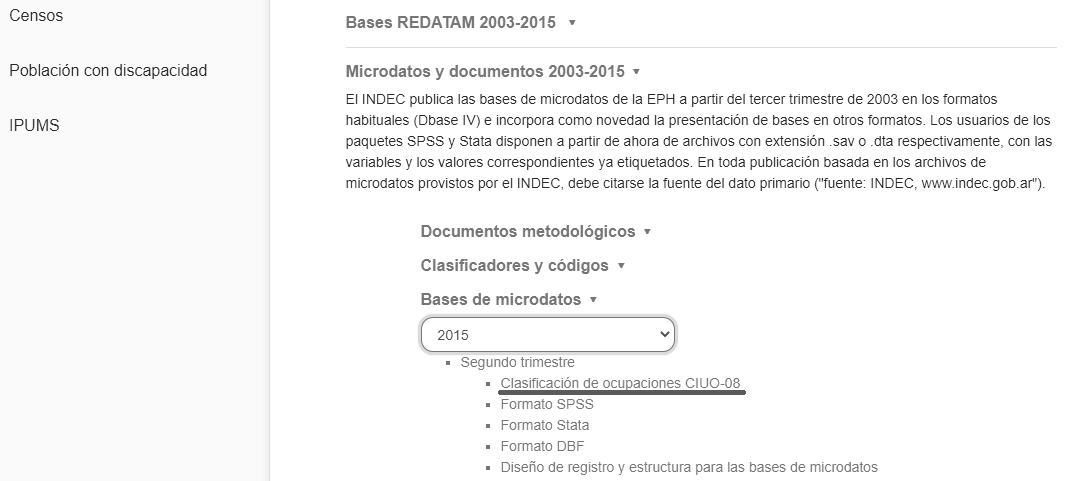
\includegraphics[width=0.8\linewidth]{imagenes/indec_ciuo} 

}

\caption{Ejemplo clasificación de Actividades Profesionales, Científicas y Técnicas - CAES 1.0 [@INDEC2011d]}\label{fig:unnamed-chunk-41}
\end{figure}

Luego de descargado el archivo, descomprimiremos el \texttt{.rar} y utilizaremos el archivo \texttt{eph\_ciuo\_215.dbf}. A continuación abriremos dicho archivo y ``pegaremos'' la variable \textbf{PP04D\_CIUO} en la base \textbf{eph\_ind\_215}. Utilizaremos las variables \textbf{CODUSU} (identificador de vivienda), \textbf{NRO\_HOGAR} (identificador del hogar) y \textbf{COMPONENTE} (identificador de miembro del hogar) como ID para emparejar ambas bases.

\begin{Shaded}
\begin{Highlighting}[]
\FunctionTok{library}\NormalTok{(foreign)}
\NormalTok{eph\_ciuo\_215 }\OtherTok{\textless{}{-}} \FunctionTok{read.dbf}\NormalTok{(}\StringTok{"bases/eph\_ciuo\_215.dbf"}\NormalTok{)  }\CommentTok{\#carga de base CIUO}
\NormalTok{eph\_ciuo\_215 }\OtherTok{\textless{}{-}}\NormalTok{ eph\_ciuo\_215 }\SpecialCharTok{\%\textgreater{}\%}
    \FunctionTok{select}\NormalTok{(CODUSU, NRO\_HOGAR, COMPONENTE, PP04D\_CIUO)  }\CommentTok{\#selecciono las variables que necesito retener}

\NormalTok{eph\_ind\_215 }\OtherTok{\textless{}{-}}\NormalTok{ eph\_ind\_215 }\SpecialCharTok{\%\textgreater{}\%}
    \FunctionTok{left\_join}\NormalTok{(eph\_ciuo\_215, }\AttributeTok{by =} \FunctionTok{c}\NormalTok{(}\StringTok{"CODUSU"}\NormalTok{, }\StringTok{"NRO\_HOGAR"}\NormalTok{, }\StringTok{"COMPONENTE"}\NormalTok{))  }\CommentTok{\#Pego la variable CIUO a la base eph\_ind\_215}
\end{Highlighting}
\end{Shaded}

Ahora podemos etiquetar la base utilizando el comando \texttt{organize\_labels} del paquete \textbf{\texttt{eph}}:

\begin{Shaded}
\begin{Highlighting}[]
\NormalTok{eph\_ind\_215 }\OtherTok{\textless{}{-}} \FunctionTok{organize\_labels}\NormalTok{(eph\_ind\_215, }\AttributeTok{type =} \StringTok{"individual"}\NormalTok{)}

\NormalTok{eph\_ind\_215}\SpecialCharTok{$}\NormalTok{CODUSU }\OtherTok{\textless{}{-}} \FunctionTok{as.character}\NormalTok{(eph\_ind\_215}\SpecialCharTok{$}\NormalTok{CODUSU)  }\CommentTok{\#Es necesario convertir a \textquotesingle{}character\textquotesingle{} para futuras operaciones. Esto se hace porque el comando \textquotesingle{}organize\_labels\textquotesingle{} le cambia el formato a la variables.}
\end{Highlighting}
\end{Shaded}

¡Listo! La base está preparada para ser explorada.

\hypertarget{condiciuxf3n-de-actividad-1}{%
\subsubsection{Condición de actividad}\label{condiciuxf3n-de-actividad-1}}

En la \textbf{EPH} la variable que mide la \textbf{condición de actividad} puede ser encontrada bajo el nombre ``ESTADO''. Exploraremos las distintas categorías y frecuencias de casos que presenta para dicho trimestre.

\begin{Shaded}
\begin{Highlighting}[]
\FunctionTok{table}\NormalTok{(eph\_ind\_215}\SpecialCharTok{$}\NormalTok{ESTADO)}
\end{Highlighting}
\end{Shaded}

\begin{verbatim}

Entrevista individual no realizada (no respuesta al cuestionario individual) 
                                                                          63 
                                                                     Ocupado 
                                                                       24398 
                                                                  Desocupado 
                                                                        1450 
                                                                    Inactivo 
                                                                       25138 
                                                          Menor de 10 anios. 
                                                                        8979 
\end{verbatim}

Como puede observarse las categorías son \emph{entrevista individual no realizada}, \emph{ocupado}, \emph{desocupado}, \emph{inactivo} y \emph{menor de 10 años}. En el caso de que pretendamos seleccionar únicamente a la población económicamente activa, deberemos filtrar las categorías 1 (ocupado) y 2 (desocupado). En este caso nos quedaríamos con 25848 registros.

\begin{Shaded}
\begin{Highlighting}[]
\NormalTok{eph\_2015\_PEA }\OtherTok{\textless{}{-}}\NormalTok{ eph\_ind\_215 }\SpecialCharTok{\%\textgreater{}\%}
    \FunctionTok{filter}\NormalTok{(ESTADO }\SpecialCharTok{==} \DecValTok{1} \SpecialCharTok{|}\NormalTok{ ESTADO }\SpecialCharTok{==} \DecValTok{2}\NormalTok{)}

\FunctionTok{nrow}\NormalTok{(eph\_2015\_PEA)}
\end{Highlighting}
\end{Shaded}

\begin{verbatim}
[1] 25848
\end{verbatim}

\hypertarget{ocupaciuxf3n-1}{%
\subsubsection{Ocupación}\label{ocupaciuxf3n-1}}

Como presentaremos en la próxima unidad, la ocupación es la variable central en la construcción de esquemas de estratificación y clases sociales. En el caso de la EPH, los censos (posteriores a 1991) y las diversas encuestas que produce el \textbf{INDEC}, en las que se releva información ocupacional, suelen codificar dicha variable a través del \textbf{CNO}.

La \textbf{EPH} recaba la ocupación tanto para la población ocupada como desocupada, relevando para este último grupo el dato de la última ocupación realizada, en el caso que hubiera existido. Mientras que el primer dato se guarda en la variable \emph{PP04D\_COD}, la última ocupación de los desocupados puede encontrarse en la variable \emph{PP11D\_COD}. Con el comando \texttt{table} podemos visualizar todos los códigos existentes en la base y su frecuencia absoluta.

\begin{Shaded}
\begin{Highlighting}[]
\FunctionTok{table}\NormalTok{(eph\_ind\_215}\SpecialCharTok{$}\NormalTok{PP04D\_COD)}
\end{Highlighting}
\end{Shaded}

\begin{verbatim}

      00001 01001 02001 03001 04001 05001 05002 06001 06002 07001 10112 10113 
35630    44     2    11    66    11   102   654   266     1     6    26    13 
10122 10131 10132 10133 10201 10202 10203 10311 10312 10313 10314 10323 10331 
    1     2    12     8    12    53    60    11   136   118    31     2    29 
10332 10333 11113 11131 11132 11202 11203 11311 11312 11313 11323 11331 11332 
   33  2127     1   108     2     2     3    10     4     6     1   112     4 
11333 20111 20112 20113 20131 20132 20133 20202 20203 20311 20312 20313 20314 
   52     1     1     9    57     2     7    10    25     8     7   203     6 
20323 20331 20332 20333 30111 30112 30113 30131 30132 30133 30202 30203 30311 
    1    94    67   354     2    74   930     3     1     9     1    71     8 
30312 30313 30314 30323 30331 30332 30333 31113 31312 31313 31314 32111 32113 
  217   310  1018     1     4     2    23    58     2   148     3     1     1 
32123 32131 32133 32201 32202 32311 32312 32313 32314 32323 32333 33113 33133 
    1     2     1     1     5     1     2     5   152     2    10   217     1 
33312 33313 33314 33333 34113 34123 34202 34203 34312 34313 34314 34323 34324 
    2     8    20     3     3   241     6     9     5    15    30   939     4 
34331 34332 34333 35113 35123 35131 35201 35202 35203 35313 35314 35323 35333 
    1     2     1     4    20     2     2     1     6    11    28   176     7 
36113 36203 36313 36314 36323 36333 40111 40112 40113 40131 40132 40201 40202 
   13    16    57   104    59    70    77    57     2     5     2     4    17 
40203 40311 40312 40313 40314 40322 40323 40331 40332 40333 41111 41112 41113 
    1   251   400    12    19    27     9    23    12     1     2   112     1 
41201 41202 41203 41311 41312 41313 41314 41323 41331 41332 41333 42131 42201 
    5    10    14   115  1335    98     1     2    12     1     2     1     1 
42202 42203 42311 42313 42331 42332 42333 43111 43112 43131 43311 43331 43332 
    1     4     4     7    39     5     6     1     2    22     1    40     4 
44111 44112 44113 44131 44132 44203 44312 44313 44331 45111 45112 45122 45123 
    1     3     2     2     1     3    41    10     2     1     3     3     1 
45131 45132 45203 45311 45312 45322 45323 45331 45332 45662 46112 46202 46203 
    5     3     1    11    34     8     2     7    30     1     3     3     1 
46311 46312 46313 46314 46331 46332 46333 47113 47203 47312 47313 47314 47323 
   18    52    17     2     3     1     2     5     7     1   255    71     6 
48203 48311 48312 48313 48323 49202 49203 49311 49312 49313 49314 49323 49331 
    5    27    65   309    14     1     1     3    14    53     4     5     1 
50111 50112 50113 50122 50131 50311 50312 50313 50322 51112 51202 51203 51312 
   22     1     2     1     2    25     2     2     1    30     2     1    77 
51314 51331 52112 52113 52123 52203 52312 52313 52314 52323 52332 52333 53112 
    3     1     3     2     4     3    13    20     2     5     4     3     2 
53113 53203 53312 53313 53314 53323 54112 54133 54311 54312 54313 54323 54332 
  160    31     9   262   286     3     4     1     1    10    14     1     2 
54333 55203 55312 55314 56113 56123 56203 56313 56314 56323 57112 57113 57312 
   12     3     1  1354    22     1     7    67   927    21     9   130     3 
57313 57314 58112 58113 58132 58203 58312 58313 58314 58323 58332 59313 60111 
   30   437    11   128     1     1     8   108    13     2     2     1     2 
60113 60123 60131 60203 60311 60312 60313 60314 60323 60331 60332 60333 61113 
    1     4     6     2     1     1    50     3    11     5     1     1     4 
61123 61203 61311 61313 61314 61323 61331 62313 62314 62323 63113 63313 63331 
    2     1     1    10     2     1     1     5     1     4     1     2     2 
64113 64202 64313 64314 64323 64331 70131 70202 70203 70311 70312 70313 70322 
    1     1     8     2     2     1     2     3    28     1     3    33     2 
70323 70331 70332 70333 71113 71201 71202 71203 71311 71312 71313 71323 71331 
   27     8     2     1     1     2     1    10     1     3     9    12     6 
71332 71333 72112 72113 72131 72132 72201 72202 72203 72311 72312 72313 72314 
    1     1    29   873    50     1     2     3    58     2    60  1068   576 
72323 72331 72332 72333 73113 74314 80111 80112 80113 80123 80131 80132 80202 
   41    56    17     2     1     1     1    74   144   222     5     1     4 
80203 80311 80312 80313 80314 80322 80323 80331 80332 80333 81101 81121 81123 
   64     4    24   516    63     4   688    21     2    10     1     1     2 
81131 81132 81201 81202 81323 81331 81332 81333 82111 82112 82113 82123 82131 
   23     3    19     1     1    68     9     1     1    46   219    49     1 
82203 82312 82313 82314 82323 90112 90113 90203 90312 90313 90323 90331 90332 
    2    23   192    32     7     4     5     6    14    76     6     1     2 
91311 92112 92113 92132 92202 92203 92312 92313 92331 92333 99999 
    1    44     3     2     1     1    90    48     2     1    53 
\end{verbatim}

Por otro lado, el paquete \textbf{\texttt{eph}} mediante la función \texttt{organize\_CNO} nos agrega 4 columnas a la base en donde se clasifica cada componente del CNO: carácter, jerarquía, tecnología y calificación ocupacional. A continuación revisamos dicho comando y solicitaremos las frecuencias, por ejemplo, de la calificación.

\begin{Shaded}
\begin{Highlighting}[]
\NormalTok{eph\_ind\_215 }\OtherTok{\textless{}{-}} \FunctionTok{organize\_cno}\NormalTok{(}\AttributeTok{base =}\NormalTok{ eph\_ind\_215)}

\FunctionTok{table}\NormalTok{(eph\_ind\_215}\SpecialCharTok{$}\NormalTok{CALIFICACION)}
\end{Highlighting}
\end{Shaded}

\begin{verbatim}

No calificados          Ns.Nc     Operativos  Profesionales       Técnicos 
          5195             53          12879           2012           4259 
\end{verbatim}

Por su parte en la variable \emph{PP04D\_CIUO} encontraremos a la ocupación codificada según el \textbf{CIUO}.

\begin{Shaded}
\begin{Highlighting}[]
\FunctionTok{table}\NormalTok{(eph\_ind\_215}\SpecialCharTok{$}\NormalTok{PP04D\_CIUO)}
\end{Highlighting}
\end{Shaded}

\begin{verbatim}

0110 0210 0310 1111 1112 1114 1120 1211 1212 1213 1219 1221 1222 1223 1311 1321 
   4   10   34    4   45    7   34    5    4    1    6   45    1    1    7    5 
1322 1323 1324 1330 1341 1342 1343 1344 1345 1346 1349 1411 1412 1420 1431 1439 
   1   14   12    5    1    8    2    1   76   15    6    5   24   68    1   14 
2111 2112 2113 2114 2120 2131 2132 2133 2141 2142 2143 2144 2145 2146 2149 2151 
   1    3    1    6    1   38   20    5   17   33    4    4    6    2    3    8 
2152 2153 2161 2163 2164 2165 2166 2211 2212 2221 2240 2250 2261 2262 2263 2265 
   5    2   80    9    1   10   21  121  110    3    2   19   58   30    6    3 
2266 2269 2310 2320 2330 2341 2342 2351 2352 2353 2354 2355 2356 2359 2411 2412 
   5    9  164   39  426  487  177   20   50   24   27   34    4   83  189   14 
2413 2421 2422 2423 2424 2431 2432 2433 2434 2511 2512 2513 2514 2519 2521 2522 
   2    5   19   51   11    8    3    7    1   33   20   22    9    2    4    8 
2523 2529 2611 2612 2619 2622 2631 2632 2633 2634 2635 2636 2641 2642 2643 2651 
   9    2  242   10    1    3   11    2    1   86   26   12    3   54    5    5 
2652 2653 2654 2655 2656 2659 3111 3112 3113 3114 3115 3116 3117 3118 3119 3121 
  21    2    6    8   17    3   13   29   12   25    6    3    7    8    4   23 
3122 3123 3131 3132 3133 3134 3135 3139 3141 3142 3143 3152 3153 3154 3155 3211 
  71   92   21   14    3   14    1   18    6    2    1    4    2    3    3   40 
3212 3213 3214 3221 3222 3240 3251 3252 3253 3254 3255 3256 3257 3258 3259 3311 
  37   10   16  257    2    2    6    4    3    6   52   11   54    3    1   15 
3312 3313 3314 3315 3321 3322 3323 3324 3331 3332 3333 3334 3339 3341 3342 3343 
  34   77    8    6   47   72   14   66    9   17    5   40   47  109   32   91 
3344 3351 3352 3353 3354 3355 3359 3411 3412 3413 3421 3422 3423 3431 3432 3434 
  27    1    9    3   10    9    9   36   55    5    7   34  104   23   11   17 
3435 3511 3512 3513 3514 3521 3522 4110 4120 4131 4132 4211 4212 4214 4221 4222 
  33   23   13   19    9   30    8 1830  226    5   24   21   59   29   27   81 
4223 4224 4225 4226 4227 4229 4311 4312 4313 4321 4322 4323 4411 4412 4413 4415 
  38   25   29   64    9    4  289    9   18  119   17   35   26   70    1    3 
4416 4419 5111 5112 5113 5120 5131 5132 5141 5142 5151 5152 5153 5161 5162 5163 
   6   20    1    3   15  301  146   36  155   42    7    4   52    2    5    6 
5164 5165 5169 5211 5212 5221 5222 5223 5230 5241 5242 5243 5244 5245 5246 5249 
  23    1    6   69   33 1122   93 1229  230    2    7  241   41   47   36    8 
5311 5312 5321 5322 5329 5411 5412 5413 5414 5419 6111 6112 6113 6114 6121 6122 
 265  106   62  147   57   10  413   42  344   42    9    6   10   11   27    3 
6123 6130 6210 6222 6223 7111 7112 7113 7114 7115 7119 7121 7122 7123 7125 7126 
   2    5    6    5    6    5 1240    3    4   58    3   10    8   11   11  163 
7127 7131 7132 7211 7212 7213 7214 7215 7221 7222 7223 7224 7231 7232 7233 7234 
  39  177   31    2  126   74   17    2  108   23   34    3  318   14  141   14 
7311 7312 7313 7314 7315 7316 7317 7318 7319 7321 7322 7323 7411 7412 7413 7421 
   3    3    4   10    5    9   22   63   25   19   52   13  185   73   44   28 
7422 7511 7512 7513 7514 7515 7516 7521 7522 7523 7531 7532 7533 7534 7535 7536 
 111   54  115    7    1    9    1    4   74    3   73   10   63   27    1   40 
7542 7543 7544 7549 8111 8112 8113 8114 8121 8122 8131 8132 8141 8142 8143 8151 
   2   34    9    9    3    3   37   12   44   14   17    2   28   35   13   21 
8152 8153 8154 8155 8156 8157 8159 8160 8172 8181 8182 8183 8189 8211 8212 8219 
  12   73    5    2   18   23   24  102   30   19    2   53    5   28   88   18 
8311 8312 8321 8322 8331 8332 8341 8342 8343 8344 8350 9111 9112 9121 9122 9123 
  10    9   49  758  179  242   18   25   24   58    6 1361  763   11   75    1 
9129 9211 9212 9213 9214 9215 9311 9312 9313 9321 9329 9331 9333 9334 9411 9412 
   2   28   14    1  190    3    6   13  561   61   47    5  158  146   36  138 
9510 9520 9611 9612 9613 9621 9622 9623 9624 9629 9999 
   8  113   45   41  108   32  123    7    1   21   41 
\end{verbatim}

A través del paquete \textbf{\texttt{modest}} y el comando \texttt{mfv} (most frequent value) calcularemos la moda de dichas variables, es decir, la ocupación más repetida en el relevamiento.

\begin{Shaded}
\begin{Highlighting}[]
\NormalTok{modeest}\SpecialCharTok{::}\FunctionTok{mfv}\NormalTok{(eph\_ind\_215}\SpecialCharTok{$}\NormalTok{PP04D\_CIUO, }\AttributeTok{na.rm =} \ConstantTok{TRUE}\NormalTok{)}
\end{Highlighting}
\end{Shaded}

\begin{verbatim}
[1] 4110
411 Levels: 0110 0210 0310 1111 1112 1114 1120 1211 1212 1213 1219 1221 ... 9999
\end{verbatim}

El código 4110 designa a los \textbf{oficinistas generales}

\hypertarget{rama-de-actividad-1}{%
\subsubsection{Rama de actividad}\label{rama-de-actividad-1}}

Al igual que para el caso de la ocupación, la rama de actividad es computada tanto para la población ocupada como la desocupada. En los relevamientos previos a 2011 y posteriores a 2016, en el primer caso acudimos a la variable \emph{PP04B\_COD} mientras que en el segundo a la \emph{PP11B\_COD}. Para los relevamiento entre 2011 y 2015, dichas variables fueron nombradas sin el sufijo *\_COD* y con el sufijo *\_CAES*.

Echamos un vistazo a la distribución de la población ocupada según la rama de actividad.

\begin{Shaded}
\begin{Highlighting}[]
\FunctionTok{table}\NormalTok{(eph\_ind\_215}\SpecialCharTok{$}\NormalTok{PP04B\_CAES)}
\end{Highlighting}
\end{Shaded}

\begin{verbatim}

       0101  0102  0103  0104  0200  0300  0600  0700  0800  0900  1001  1002 
35630   101    43    35     1     6    15    48     4    26   100   116    43 
 1003  1009  1100  1200  1300  1400  1501  1502  1600  1700  1800    19  1902 
   37   383    53     5   120   156    13    57    41    31    67     3     8 
   20  2001  2002  2009  2100  2201  2202  2301  2309  2400  2500  2601  2602 
   24     6    30     5   101    33    62    14    63    26   406    18     7 
 2603  2604  2701  2709  2800  2900  3001  3003  3009  3100  3200  3300  3501 
   24    26    34    32    94    68     8     2    22   179   110   104   101 
 3502  3600  3800  3900  4000  4501  4502  4503  4504    48  4801  4802  4803 
   19    53   113     3  2575   100   398    74    48   126    21    35   777 
 4804  4805  4806  4807  4808  4809  4810  4811    49  4901  4902  4903  4904 
  427   168    80   651   827    41   416    28    15    36     1   582   302 
 4909  5000  5100  5201  5202  5300  5500  5601  5602  5800  5900  6000  6100 
   36    14    15    34   168   114   102   669    42    37    23    54   158 
 6200  6300  6400  6500  6600  6800  6900  7000  7100  7200  7301  7302  7400 
   95     7   219   179    12    55   371    60   136    36    40    11    91 
 7500  7701  7702  7800  7900  8000  8101  8102  8200  8401  8402  8403  8501 
   29    16     9    12    44   220   143   131   115  2094   990    76  1944 
 8509  8600  8700  8800  9000  9100  9200  9301  9302  9401  9402  9409  9501 
  229  1243    65    24    29    26   105   169    61    26    34   321    49 
 9502  9503  9601  9602  9603  9609  9700     Z 
    9   168    18   214    25    62  1780   113 
\end{verbatim}

Del mismo modo que con la ocupación, el paquete \textbf{\texttt{eph}} mediante la función \texttt{organize\_CAES} nos agrega 8 columnas a la base en donde se clasifican distintas cuestiones: versión de la CAES, código de sección y división, etiqueta de sección y división y clasificación de ramas de actividad agregadas. A continuación revisamos dicho comando y solicitaremos las frecuencias de las ramas agregadas.

\begin{Shaded}
\begin{Highlighting}[]
\NormalTok{eph\_ind\_215}\SpecialCharTok{$}\NormalTok{PP04B\_COD }\OtherTok{\textless{}{-}} \FunctionTok{as.character}\NormalTok{(eph\_ind\_215}\SpecialCharTok{$}\NormalTok{PP04B\_COD)  }\CommentTok{\#esta linea de comando corrige un error derivado del auto{-}etiquetamiento de las categorías.}
\NormalTok{eph\_ind\_215 }\OtherTok{\textless{}{-}} \FunctionTok{organize\_caes}\NormalTok{(}\AttributeTok{base =}\NormalTok{ eph\_ind\_215)}

\FunctionTok{table}\NormalTok{(eph\_ind\_215}\SpecialCharTok{$}\NormalTok{caes\_eph\_label)}
\end{Highlighting}
\end{Shaded}

\begin{verbatim}

                              Actividades primarias 
                                                379 
                            Industria manufacturera 
                                               2631 
                                       Construccion 
                                               2575 
                                           Comercio 
                                               4217 
                             Hoteles y restaurantes 
                                                813 
        Transporte, almacenamiento y comunicaciones 
                                               1691 
 Servicios financieros, de alquiler y empresariales 
                                               1929 
 Administracion publica, defensa y seguridad social 
                                               3084 
                                          Ensenanza 
                                               2173 
                      Servicios sociales y de salud 
                                               1332 
                                 Servicio domestico 
                                               1780 
Otros servicios comunitarios, sociales y personales 
                                               1316 
                                        Otras ramas 
                                                169 
                  Actividades no bien especificadas 
                                                120 
\end{verbatim}

\hypertarget{categoruxeda-de-ocupaciuxf3n-1}{%
\subsubsection{Categoría de ocupación}\label{categoruxeda-de-ocupaciuxf3n-1}}

La categoría de ocupación es una variable que también es de vital importancia en la construcción de clasificaciones. La misma puede encontrarse bajo el nombre de \emph{CAT\_OCUP}. A continuación exploramos sus categorías:

\begin{Shaded}
\begin{Highlighting}[]
\FunctionTok{table}\NormalTok{(eph\_ind\_215}\SpecialCharTok{$}\NormalTok{CAT\_OCUP)}
\end{Highlighting}
\end{Shaded}

\begin{verbatim}

                                   0                               Patron 
                               34530                                  969 
                       Cuenta propia                    Obrero o empleado 
                                4772                                19597 
Trabajador familiar sin remuneracion 
                                 160 
\end{verbatim}

\hypertarget{sector-de-actividad-1}{%
\subsubsection{Sector de actividad}\label{sector-de-actividad-1}}

En la \textbf{EPH} el sector de actividad puede encontrarse en la variable \emph{PP04A}.

\begin{Shaded}
\begin{Highlighting}[]
\FunctionTok{table}\NormalTok{(eph\_ind\_215}\SpecialCharTok{$}\NormalTok{PP04A)}
\end{Highlighting}
\end{Shaded}

\begin{verbatim}

              0      ...estatal      ...privada ...de otro tipo        Ns./Nr.. 
          35630            5517           18492             373              16 
\end{verbatim}

\hypertarget{tamauxf1o-del-establecimiento-1}{%
\subsubsection{Tamaño del establecimiento}\label{tamauxf1o-del-establecimiento-1}}

La medición del tamaño del establecimiento se encuentra distribuida en dos variables: \emph{PP04C} y \emph{PP04C99}. La primera permite captar en forma detallada el tamaño del establecimiento donde trabaja la persona en diferentes rangos, mientras que la segunda permite recuperar, mediante una clasificación más acotada, aquel dato que en la primera variable figuraba como ``Ns/Nc''. A continuación exploramos ambas variables en forma cruzada.

\begin{Shaded}
\begin{Highlighting}[]
\FunctionTok{table}\NormalTok{(eph\_ind\_215}\SpecialCharTok{$}\NormalTok{PP04C, eph\_ind\_215}\SpecialCharTok{$}\NormalTok{PP04C99)}
\end{Highlighting}
\end{Shaded}

\begin{verbatim}
                       
                            0 hasta 5 de 6 a 40 mas de 40 Ns./Nr..
  0                     37370       0         0         0        0
  1 persona              3565       0         0         0        0
  2 personas             2123       0         0         0        0
  3 personas             1241       0         0         0        0
  4 personas              816       0         0         0        0
  5 personas              752       0         0         0        0
  6 a 10 personas        1876       0         0         0        0
  11 a 25 personas       1783       0         0         0        0
  26 a 40 personas       1567       0         0         0        0
  de 41 a 100 personas   2035       0         0         0        0
  de 101 a 200 personas  1386       0         0         0        0
  de 201 a 500 personas  1204       0         0         0        0
  mas de 500 personas    1304       0         0         0        0
  Ns./Nr.                   0     125       610       919     1352
\end{verbatim}

Al igual que en el caso de la ocupación y la rama de actividad, para aquellas personas desocupadas que han trabajado alguna vez en el pasado, el tamaño del establecimiento puede ser identificado en las variables \emph{PP11C} y \emph{PP11C99}.

\hypertarget{supervisiuxf3n-1}{%
\subsubsection{Supervisión}\label{supervisiuxf3n-1}}

Si bien la supervisión no es una variable medida directamente en la \textbf{EPH}, podemos aproximarnos a dicha noción a través del \textbf{CNO}. En su tercer dígito mide la jerarquía ocupacional. Sin embargo, para extraer dicha información es necesario ``partir'' el código ocupacional, reteniendo el tercer dígito. A través de \textbf{\texttt{R}}, realizaremos la operación utilizando la función \texttt{str\_sub} del paquete \textbf{\texttt{stringr}}, indicando que dígitos queremos retener. En este caso debemos señalar que queremos retener únicamente el tercer dígito (que empiece en el 3 y termine en el 3) y se lo asignaremos a una nueva variable llamada ``cno\_jerarquia''.

\begin{Shaded}
\begin{Highlighting}[]
\NormalTok{eph\_ind\_215}\SpecialCharTok{$}\NormalTok{cno\_jerarquia }\OtherTok{\textless{}{-}} \FunctionTok{str\_sub}\NormalTok{(eph\_ind\_215}\SpecialCharTok{$}\NormalTok{PP04D\_COD, }\AttributeTok{start =} \DecValTok{3}\NormalTok{, }\AttributeTok{end =} \DecValTok{3}\NormalTok{)}

\NormalTok{eph\_ind\_215 }\SpecialCharTok{\%\textgreater{}\%}
    \FunctionTok{filter}\NormalTok{(cno\_jerarquia }\SpecialCharTok{==} \DecValTok{2}\NormalTok{) }\SpecialCharTok{\%\textgreater{}\%}
    \FunctionTok{nrow}\NormalTok{()}
\end{Highlighting}
\end{Shaded}

\begin{verbatim}
[1] 619
\end{verbatim}

Conociendo que el código 2 es el que hace referencia a la jefatura, si filtramos los resultados podemos decir que existen 619 casos que supervisan las tareas de otras personas.

\hypertarget{clases5}{%
\section{Los Nomencladores de clases sociales}\label{clases5}}

Este capítulo tiene como propósito presentar los diversos abordajes teórico-empíricos más utilizados en el estudio de la estratificación social, a nivel internacional y nacional, fundamentalmente desde una mirada operacional.

Presentados ya los principales enfoque teóricos en el \protect\hyperlink{estructura1}{Capítulo 2}, en esta sección se focaliza en las operaciones que se realizan desde el punto de vista metodológico, siguiendo criterios teóricos, para hacer posible la medición de estratos y clases sociales definidas en términos conceptuales. Para esto revisaremos algunas de las propuestas más utilizadas.

Estas preguntas guian el capítulo:\\
- ¿Qué enfoques teóricos sobre las clases sociales fueron operacionalizados empíricamente?\\
- ¿Qué diferencias presentan dichos enfoques?\\
- ¿Qué cuestiones aportan los enfoques nacionales?\\
- ¿Cómo se operacionalizan los esquemas presentados?\\
- ¿Cuáles son las limitaciones que presentan las fuentes de datos nacionales en la aplicación de dichos esquemas?\\
- ¿Sobre cuáles unidades de análisis podemos trabajar en el estudio de las clases sociales?

Al finalizar el capítulo se espera que los lectores puedan:

\begin{enumerate}
\def\labelenumi{\arabic{enumi}.}
\tightlist
\item
  Identificar las semejanzas y diferencias específicas que presenta cada nomenclador de clases propuesto por los autores aquí revisados.
\item
  Conocer cuáles son las principales variables que sustentan a cada esquema.
\item
  Adquirir la práctica en la operacionalización de variables complejas como la clase social.
\item
  Establecer críticamente qué esquema utilizar según el marco teórico propuesto.
\end{enumerate}

Para una mayor comprensión del capítulo recomendamos la lectura de los siguientes documentos:

\begin{itemize}
\item
  Clemenceau, L., Fernández Melián, M. C., y Rodríguez de la Fuente, J. (\protect\hyperlink{ref-Clemenceau.etal2016}{2016}). Análisis de esquemas de clasificación social basados en la ocupación desde una perspectiva teórica-metodológica comparada. Documentos de Jóvenes Investigadores IIGG, 44.
\item
  Francés García, F. J. (\protect\hyperlink{ref-FrancesGarcia2009}{2009}). Elementos para el estudio de la estratificación social en las sociedades avanzadas: Estrategias operativas. Revista Obets, 3.
\item
  Torrado, S. (\protect\hyperlink{ref-Torrado1998d}{1998b}). La medición empírica de las clases sociales. En Familia y diferenciación social. Buenos Aires: Eudeba.
\item
  Sacco, N. (\protect\hyperlink{ref-Sacco2019}{2019}). Estructura social de la Argentina, 1976-2011. Trabajo y sociedad, (32), 25--51, (Anexo metodológico).
\item
  Carabaña, J. (\protect\hyperlink{ref-Carabana1997}{1997}). Esquemas y estructuras. Revista crítica de ciências sociais, (49), 67-91.
\item
  Barozet, E. (\protect\hyperlink{ref-Barozet2007}{2007}). La variable ocupación en los estudios de estratificación social.
\item
  Sautu, R., Dalle, P., Otero, M. P., y Rodríguez, S. (\protect\hyperlink{ref-Sautu.etal2007}{2007}). La construcción de un esquema de clases a partir de datos secundarios. (Documento de Cátedra II. 4). Metodología de la Investigación Social II, Cátedra Sautu, Facultad de Ciencias Sociales-UBA.
\item
  Rodríguez de la Fuente, J. J. (\protect\hyperlink{ref-RodriguezdelaFuente2020}{2020}). Del origen de clase a las condiciones de vida actuales. Movilidad social y bienestar material en la Ciudad de Buenos Aires (2004-2015). Buenos Aires: Teseo Press. (Capítulo 2. Diseño Metodológico)
\end{itemize}

\hypertarget{computadora}{%
\subsection{De las clases en el papel a las clases en la computadora}\label{computadora}}

\hypertarget{operacionalizando-el-concepto-de-clase}{%
\subsubsection{Operacionalizando el concepto de clase}\label{operacionalizando-el-concepto-de-clase}}

El proceso de \emph{operacionalización} implica el pasaje de conceptos teórico-abstractos a indicadores empíricos, es decir, la transformación de un fenómeno no observable o latente, en observable (\protect\hyperlink{ref-DAncona1996}{D'Ancona, 1996}). Bourdieu (\protect\hyperlink{ref-Bourdieu1990}{1990}), en referencia a la conceptualización científica de las clases sociales, denominó a este proceso como la construcción de clases ``en el papel'', en tanto funcionan como \emph{constructos} que son agrupaciones probables fundadas en la posición que los individuos presentan en el espacio social. De este modo, las clases son construcciones analíticas pero bien fundadas en la realidad ya que proporcionan una explicación más completa del mayor número de diferencias observadas entre los agentes (\protect\hyperlink{ref-Bourdieu1990}{Bourdieu, 1990, p. 130}).

Estas clases-constructos no son clases equiparables a las que podemos percibir y comprender como existentes en la realidad social, aunque presenten probabilidades de serlo. Ejemplificando, si nuestro esquema de clasificación nos indica que un individuo asalariado y administrativo de un organismo estatal, forma parte de la ``clase media'', eso no significa que esa categoría de clase tenga una relación directa con lo que en la realidad los propios individuos identifican como clase media (que de por sí presenta una gran heterogeneidad), ni con lo que las propias teorías pueden entender como ``clase media'' .

Las clases sociales son una parte de lo que normalmente conceptualizamos como ``estructura social''. En tanto parte, el proceso de operacionalización, es decir, de separación de aspectos que suelen estar integrados (tales como la clase, el género, los vínculos sociales, la acción política, entre otros), implica una abstracción y un recorte realizado sobre la realidad, pero que permite un acercamiento a la comprensión de la misma:

\begin{quote}
Como hemos visto, los esquemas de clase son en realidad el producto de la disolución de las estructuras sociales. La fórmula para su producción podría ser algo como lo que sigue: tómense estructuras cuyos elementos son individuos, roles o acciones cualesquiera, rómpase las relaciones que haya entre sus miembros de modo que estos queden flotando libremente y sométase el magma resultante a centrifugación hasta que se haya reunido los elementos homogéneos. Una vez terminado el proceso, calcúlense los porcentajes. Se obtiene así una descripción de la estructura social (\protect\hyperlink{ref-Carabana1997}{Carabaña, 1997, p. 85}).
\end{quote}

Resumiendo, si la estructura de clases es un aspecto de la estructura social, los esquemas de medición de clase son una aproximación al estudio de las mismas. Aunque se construyen a partir de la teoría, no deben entenderse como ``puentes directos'' entre ambos ámbitos, sino más bien como constructos estadísticos elaborados por los investigadores para aproximarse a la realidad a partir de los datos.

\hypertarget{clases-grupos-estratos-quuxe9-medimos-cuando-analizamos-la-estructura-social}{%
\subsubsection{Clases, grupos, estratos ¿Qué medimos cuando analizamos la estructura social?}\label{clases-grupos-estratos-quuxe9-medimos-cuando-analizamos-la-estructura-social}}

Es común intercambiar los conceptos cuando nos referimos al estudio de agregados poblacionales que conforman la estructura social: a veces las llamamos clases, otras veces estratos, grupos, sectores, entre otras nominaciones. Sin embargo, más allá de la intercambiabilidad de algunos términos, cada concepto corresponde a una tradición teórica y, por ende, cada concepto pone el eje en un aspecto de la realidad. Mientras que la estratificación alude en mayor medida a la idea de jerarquía y distancia entre los componentes de la misma, la idea de clase referencia a las relaciones y mutua dependencia que se establece entre los agrupamientos. Sin embargo, la mayor parte de estos enfoques, en términos operativos, se centran en la \textbf{ocupación} como principal variable desde donde construir clasificaciones (\protect\hyperlink{ref-Barozet2007}{Barozet, 2007}; \protect\hyperlink{ref-FrancesGarcia2009}{Francés García, 2009}), tal como hemos estudiado en el \protect\hyperlink{ocupacion}{Capítulo 5}.

Las bifurcaciones en la construcción de las clasificaciones comienzan a partir de los distintos criterios y decisiones llevadas adelante por los investigadores para observar a los grupos sociales (\protect\hyperlink{ref-FrancesGarcia2009}{Francés García, 2009, pp. 49--502}). Podemos citar, al menos, los siguientes aspectos a tener en cuenta:

\begin{itemize}
\item
  \emph{Elección de las medidas}: es decir, si los agrupamientos se mostraran como medidas continuas o categóricas. Mientras que el primer tipo apunta a una concepción de la estructura en tanto \emph{continumm}, en la que las distintas posiciones se diferencian en función de su distancia, el segundo aspecto, que es característico de los enfoques de clase, hace referencia a una realidad social fragmentada en grupos que adquieren su identidad a partir de su relación con los demás grupos.
\item
  \emph{Naturaleza de la información}: aquí aludimos a referentes objetivos o subjetivos. En el primer caso, son indicadores tales como la ocupación, los ingresos, el nivel educativo, etc. En cambio, los principales indicadores subjetivos de estratificación se asocian a las valoraciones subjetivas que los individuos hacen sobre las ocupaciones, que permiten la construcción de escalas de prestigio o estatus social.
\item
  \emph{Objeto de la medición}: finalmente, nos referimos a lo que realmente queremos medir a través de las herramientas elaboradas. Por un lado encontramos escalas que pretenden medir el prestigio o el estatus, otras que intentar medir la clase social y, por último, la posición socioeconómica. Cada una presentará una naturaleza distinta y apuntará a aspectos teóricos diferenciados y hasta enfrentados.
\end{itemize}

\hypertarget{clases6}{%
\subsection{Enfoques operacionalizables de clases y estratos sociales}\label{clases6}}

En el \protect\hyperlink{estructura1}{Capítulo 2} repasamos brevemente algunas de las teorías más importantes en el campo del estudio de las clases y la estratificación social. En este apartado nos enfocaremos en el proceso que dichos investigadores atravesaron para llevar las clases de la teoría a los papeles (o bien, a la computadora). De esta forma, nos preguntamos:

\begin{itemize}
\tightlist
\item
  ¿Qué decisiones han tenido que tomar?
\item
  ¿Qué limitaciones han encontrado en el pasaje de la teoría a lo empírico?
\item
  ¿Qué variables utilizaron para llevar a cabo dicho trabajo? ¿Cómo las combinaron?
\item
  ¿Qué limitaciones presentan las propuestas en función de las fuentes de datos disponibles en Argentina?
\end{itemize}

Como veremos el trabajo de desentrañar las decisiones que llevaron adelante los investigadores en la elaboración de esquemas y escalas de estratificación social no siempre es una tarea sencilla, y depende en gran medida de las huellas y directrices que los propios autores han dejado en sus trabajos acerca de cómo generar dichos constructos. Algunos han elaborado anexos, trabajos o publicaciones específicas en donde han señalado cómo construir dichos instrumentos. Otros, en cambio, han sido más ambiguos en sus formulaciones metodológicas, generando que aquellos interesados en la utilización de sus enfoques elaboren esquemas aproximados.

En este sentido, proponemos un repaso de las principales decisiones, criterios y características que asumen las clasificaciones más utilizadas tanto a nivel internacional como nacional en el estudio de las clases y la estratificación social. Vale decir que esta revisión lejos está de ser exhaustiva de todos los enfoques, por esta razón, hacia el final de este apartado listaremos algunas referencias para quien desee explorar en otros formatos clasificatorios.

\hypertarget{esquemas-internacionales}{%
\subsubsection{Esquemas internacionales}\label{esquemas-internacionales}}

\hypertarget{esquema-egp}{%
\paragraph{Esquema EGP}\label{esquema-egp}}

El esquema EGP (\protect\hyperlink{ref-Erikson.etal1979}{Erikson, Goldthorpe, \& Portocarero, 1979}) es uno de los más utilizados, tanto en términos internacionales como regionales, para el estudio de la estructura de clases como de la movilidad social. John Goldthorpe fue quien se encargó de popularizarlo a través de sus investigaciones, llegando a ser utilizado, a partir de una adaptación, por la \emph{European Statistical Office} como clasificación oficial (\emph{European Socio-economic Classification}) \footnote{\url{https://doi.org/10.1080/14616690701336518}}.

Según el autor, el esquema no debe considerarse como un mapa definitivo de la estructura de clases, sino como un instrumento de trabajo que puede sufrir cambios y modificaciones. En la construcción del mismo, intervinieron tanto ideas teóricas como consideraciones prácticas que dependieron del contexto en el que tuvo origen, de los propósitos y de la naturaleza de la información sobre la que sería aplicado (\protect\hyperlink{ref-Erikson1992}{Erikson \& Goldthorpe, 1992, p. 32}).

En referencia a los criterios operacionales que implica la construcción del esquema, se consideran (\protect\hyperlink{ref-Mendez.Gayo2007}{Méndez \& Gayo, 2007, p. 146}):\\
1. la propiedad de los medios de producción,\\
2. la existencia y número de empleados (para aquellos que no son asalariados),\\
3. la distinción no manual -- manual -- agrícola, y\\
4. el tipo de relación de empleo (de servicios o relación contractual).

En la siguiente esquema se detallan los principales criterios de clasificación y la asignación de las clases.

De esta forma, la primera gran división ocurre a nivel de relaciones de producción, diferenciando entre empleadores (\emph{employers}), trabajadores autónomos (\emph{self-employed workers}) y empleados (\emph{employees}). Para el caso de los empleadores se diferencia además según si presentan empresas grandes o pequeñas, así como por su rama de actividad (industria o agricultura), al igual que en los trabajadores autónomos. La operacionalización se complica al desagregar el mundo asalariado. Aquí interviene el criterio del tipo de \textbf{relaciones de empleo}.

La \textbf{relación de servicio} da lugar a lo que el autor denomina ``clase de servicios'' y que esta conformada por empleados profesionales, administradores y directivos. Los contratos suelen pautarse a largo tiempo y el modo de intercambio empleador-empleado suele ser difuso, en el sentido que no sólo actúa el salario como forma de pago, sino que también ciertos elementos prospectivos (aumentos, seguros sociales, pensiones, etc.) que garantizan la estabilidad y el sostenimiento del empleo. El empleado ``de servicios'' obtiene autonomía y discrecionalidad, dependiendo su rendimiento del ``acuerdo moral'' que existe con el empleador y no de sanciones externas. En contraposición, la relación basada en el \textbf{contrato de trabajo}, remite a lo que en términos agregados puede entenderse como ``clase obrera''. A diferencia de la relación de servicio, los contratos suelen ser de menor término y se realiza un intercambio de dinero por esfuerzo, calculado en función de las horas trabajadas. La discrecionalidad y autonomía suelen ser bajas, ya que el rendimiento del trabajador está atado a una mayor supervisión sobre el mismo y a condicionamientos externos en forma de sanciones. En medio de ambos tipos ideales de relaciones, se encuentran las formas mixtas que dan lugar a las clases intermedias.

Por otro lado, las clases (identificadas en el gráfico anterior a partir de números romanos) pueden clasificarse de distintos modos, en función de cuán desagregada se desee presentar la información ---Tabla \ref{tab:egp1}---. A nivel de mayor desagregación, el esquema cuenta con 11 clases, sin embargo los autores han trabajado con colapsamientos de 7, 5 y 3 clases.

\global\setlength{\Oldarrayrulewidth}{\arrayrulewidth}

\global\setlength{\Oldtabcolsep}{\tabcolsep}

\setlength{\tabcolsep}{0pt}

\renewcommand*{\arraystretch}{1.5}



\providecommand{\ascline}[3]{\noalign{\global\arrayrulewidth #1}\arrayrulecolor[HTML]{#2}\cline{#3}}

\begin{longtable}[c]{ccc}

\caption{Esquema\ de\ clases\ EGP}\label{tab:egp1}\\

\ascline{1.5pt}{666666}{1-3}

\multicolumn{1}{>{}c}{\textcolor[HTML]{000000}{\fontsize{10}{10}\selectfont{\textbf{11\ clases}}}} & \multicolumn{1}{>{}c}{\textcolor[HTML]{000000}{\fontsize{10}{10}\selectfont{\textbf{7\ clases}}}} & \multicolumn{1}{>{}c}{\textcolor[HTML]{000000}{\fontsize{10}{10}\selectfont{\textbf{5\ clases}}}} \\

\ascline{1.5pt}{666666}{1-3}\endfirsthead \caption[]{Esquema\ de\ clases\ EGP}\label{tab:egp1}\\

\ascline{1.5pt}{666666}{1-3}

\multicolumn{1}{>{}c}{\textcolor[HTML]{000000}{\fontsize{10}{10}\selectfont{\textbf{11\ clases}}}} & \multicolumn{1}{>{}c}{\textcolor[HTML]{000000}{\fontsize{10}{10}\selectfont{\textbf{7\ clases}}}} & \multicolumn{1}{>{}c}{\textcolor[HTML]{000000}{\fontsize{10}{10}\selectfont{\textbf{5\ clases}}}} \\

\ascline{1.5pt}{666666}{1-3}\endhead



\multicolumn{3}{>{}l}{\textcolor[HTML]{000000}{\fontsize{10}{10}\selectfont{Fuente:\ Erikson\ y\ Goldthorpe\ (1992)}}} \\

\endfoot



\multicolumn{1}{>{}l}{\textcolor[HTML]{000000}{\fontsize{10}{10}\selectfont{I.\ Profesionales,\ administradores\ y\ oficiales\ de\ alto\ nivel;\ Directivos\ de\ grandes\ establecimientos\ industriales;\ Propietarios\ de\ grandes\ empresas}}} & \multicolumn{1}{>{}l}{} & \multicolumn{1}{>{}l}{} \\





\multicolumn{1}{>{}l}{\textcolor[HTML]{000000}{\fontsize{10}{10}\selectfont{II.\ Profesionales,\ administradores\ y\ oficiales\ de\ bajo\ nivel;\ Directivos\ de\ pequeños\ establecimientos\ industriales;\ Supervisores\ de\ trabajadores\ no\ manuales}}} & \multicolumn{1}{>{}l}{\multirow[c]{-2}{*}{\parbox{0.75in}{\raggedright \textcolor[HTML]{000000}{\fontsize{10}{10}\selectfont{Clase\ de\ servicio\ (I\ +\ II)}}}}} & \multicolumn{1}{>{}l}{} \\





\multicolumn{1}{>{}l}{\textcolor[HTML]{000000}{\fontsize{10}{10}\selectfont{IIIa.\ Empleados\ de\ rutina\ no\ manuales\ de\ alto\ nivel\ (administración\ y\ comercio)}}} & \multicolumn{1}{>{}l}{} & \multicolumn{1}{>{}l}{} \\





\multicolumn{1}{>{}l}{\textcolor[HTML]{000000}{\fontsize{10}{10}\selectfont{IIIb.\ Empleados\ de\ rutina\ no\ manual\ de\ bajo\ nivel\ (ventas\ y\ servicios)}}} & \multicolumn{1}{>{}l}{\multirow[c]{-2}{*}{\parbox{0.75in}{\raggedright \textcolor[HTML]{000000}{\fontsize{10}{10}\selectfont{Trabajadores\ de\ rutina\ no\ manuales\ (IIIa\ +\ IIIb)}}}}} & \multicolumn{1}{>{}l}{\multirow[c]{-4}{*}{\parbox{0.75in}{\raggedright \textcolor[HTML]{000000}{\fontsize{10}{10}\selectfont{Trabajadores\ de\ cuello\ blanco\ (I\ +\ II\ +\ III)}}}}} \\





\multicolumn{1}{>{}l}{\textcolor[HTML]{000000}{\fontsize{10}{10}\selectfont{IVa.\ Pequeños\ propietarios,\ artesanos\ con\ empleados}}} & \multicolumn{1}{>{}l}{} & \multicolumn{1}{>{}l}{} \\





\multicolumn{1}{>{}l}{\textcolor[HTML]{000000}{\fontsize{10}{10}\selectfont{IVb.\ Pequeños\ propietarios,\ artesanos\ sin\ empleados}}} & \multicolumn{1}{>{}l}{\multirow[c]{-2}{*}{\parbox{0.75in}{\raggedright \textcolor[HTML]{000000}{\fontsize{10}{10}\selectfont{Pequeña\ burguesía\ (IVa\ +\ IVb)}}}}} & \multicolumn{1}{>{}l}{\multirow[c]{-2}{*}{\parbox{0.75in}{\raggedright \textcolor[HTML]{000000}{\fontsize{10}{10}\selectfont{Pequeña\ burguesía\ (IVa\ +\ IVb)}}}}} \\





\multicolumn{1}{>{}l}{\textcolor[HTML]{000000}{\fontsize{10}{10}\selectfont{IVc.\ Agricultores,\ arrendatarios\ y\ otros\ trabajadores\ cuenta\ propia\ en\ el\ sector\ agrícola}}} & \multicolumn{1}{>{}l}{\textcolor[HTML]{000000}{\fontsize{10}{10}\selectfont{Agricultores\ y\ arrendatarios\ (IVc)}}} & \multicolumn{1}{>{}l}{\textcolor[HTML]{000000}{\fontsize{10}{10}\selectfont{Trabajadores\ agrícolas\ (IVc\ +\ VIIb)}}} \\





\multicolumn{1}{>{}l}{\textcolor[HTML]{000000}{\fontsize{10}{10}\selectfont{V.\ Técnicos\ de\ nivel\ inferior,\ supervisores\ de\ trabajos\ manuales}}} & \multicolumn{1}{>{}l}{} & \multicolumn{1}{>{}l}{} \\





\multicolumn{1}{>{}l}{\textcolor[HTML]{000000}{\fontsize{10}{10}\selectfont{VI.\ Trabajadores\ manuales\ calificados}}} & \multicolumn{1}{>{}l}{\multirow[c]{-2}{*}{\parbox{0.75in}{\raggedright \textcolor[HTML]{000000}{\fontsize{10}{10}\selectfont{Trabajadores\ calificados\ (V\ +\ VI)}}}}} & \multicolumn{1}{>{}l}{\multirow[c]{-2}{*}{\parbox{0.75in}{\raggedright \textcolor[HTML]{000000}{\fontsize{10}{10}\selectfont{Trabajadores\ calificados\ (V\ +\ VI)}}}}} \\





\multicolumn{1}{>{}l}{\textcolor[HTML]{000000}{\fontsize{10}{10}\selectfont{VIIa.\ Trabajadores\ manuales\ semicalificados\ y\ no\ calificados}}} & \multicolumn{1}{>{}l}{\textcolor[HTML]{000000}{\fontsize{10}{10}\selectfont{Trabajadores\ no\ calificados\ (VIIa)}}} & \multicolumn{1}{>{}l}{} \\





\multicolumn{1}{>{}l}{\textcolor[HTML]{000000}{\fontsize{10}{10}\selectfont{VIIb.\ Trabajadores\ agrícolas}}} & \multicolumn{1}{>{}l}{\textcolor[HTML]{000000}{\fontsize{10}{10}\selectfont{Trabajadores\ agrícolas\ (VIIb)}}} & \multicolumn{1}{>{}l}{\multirow[c]{-2}{*}{\parbox{0.75in}{\raggedright \textcolor[HTML]{000000}{\fontsize{10}{10}\selectfont{Trabajadores\ no\ calificados\ (VIIa)}}}}} \\

\ascline{1.5pt}{666666}{1-3}



\end{longtable}



\arrayrulecolor[HTML]{000000}

\global\setlength{\arrayrulewidth}{\Oldarrayrulewidth}

\global\setlength{\tabcolsep}{\Oldtabcolsep}

\renewcommand*{\arraystretch}{1}

Si bien existe bibliografía (\protect\hyperlink{ref-Erikson1992}{Erikson \& Goldthorpe, 1992}; \protect\hyperlink{ref-Rose.Harrison2007}{Rose \& Harrison, 2007b}) en la que se señalan algunos indicios sobre cómo operacionalizar el esquema EGP, no hay una forma directa y unívoca de realizarlo. Goldthorpe y Heath (\protect\hyperlink{ref-Goldthorpe.Heath1992}{1992}) han realizado el ejercicio de operacionalización del mismo, pero para ser utilizado con la clasificación estandarizada de ocupaciones inglesa, que se diferencia tanto de la CIUO-88 como de la CIUO-08.

Comúnmente, los investigadores interesados en utilizar la clasificación han partido de una adaptación realizada por Ganzeboom para SPSS \footnote{\url{http://www.harryganzeboom.nl/isco88/index.htm}}, a partir del clasificador ocupacional CIUO-88. Existe un paquete para \textbf{\texttt{R}} llamado \texttt{ocuppar}, que retoma la propuesta de Ganzeboom para ser utilizada bajo dicho programa. En el apartado siguiente, a modo de ejemplo retomaremos dicha propuesta de operacionalización.

\hypertarget{esquema-de-wright}{%
\paragraph{Esquema de Wright}\label{esquema-de-wright}}

Como hemos señalado en el \protect\hyperlink{estructura1}{Capítulo 2}, Wright ha presentado dos propuestas operacionalizables de clases, desde un enfoque neo-marxista: uno basado en las posiciones de las relaciones de clase y otro de las explotaciones múltiples. En este caso presentaremos los principales criterios abordados por el autor para el desarrollo de la segunda propuesta\footnote{La propuesta de operacionalización del enfoque de posiciones contradictorias puede encontrarse en Wright (\protect\hyperlink{ref-Wright1979}{1979}).}.

Influenciado por el marxismo analítico, Wright identificó cuatro tipos de bienes de explotación posibles de ser relevamos empíricamente, y que se traducen en los diferentes tipos de derechos y poderes (recursos tangibles e intangibles) que tienen los sujetos en las relaciones de producción (\protect\hyperlink{ref-Wright2005}{Wright, 2005}):

\begin{enumerate}
\def\labelenumi{\arabic{enumi}.}
\tightlist
\item
  \textbf{Fuerza de trabajo} (explotación feudal),\\
\item
  Los \textbf{medios de producción} (explotación capitalista),\\
\item
  Los \textbf{bienes de organización} (explotación estatal) y\\
\item
  Las \textbf{cualificaciones} (explotación socialista)
\end{enumerate}

De este modo, la combinación de esos cuatro tipos de bienes de explotación, permiten la generación de 12 posiciones de clase (\protect\hyperlink{ref-Wright1994b}{Wright, 1994}).

Ahora bien, ¿Cómo llega Wright a operacionalizar dicho esquema? En este sentido, el autor es bastante franco y sincero ya que explicita todas sus decisiones y limitaciones, señalando que de este modo ``los que lo deseen puedan repetir los resultados que aquí hemos presentado, y hará también que nuestras decisiones operacionales queden lo más abiertas posibles a la crítica'' (\protect\hyperlink{ref-Wright1994b}{Wright, 1994}). Esto es de vital importancia en el campo científico, en donde la posibilidad de reproducir los resultados realizados en distintos contextos de investigación.

Es necesario aclarar que para abordar la estructura de clases desde el enfoque propuesto por Wright se torna crucial realizar un relevamiento que recabe ciertos indicadores específicos vinculados directamente con el enfoque teórico del que parte el autor \footnote{Una revisión de los items relevados por Wright para la construcción de sus indicadores específicos que constituyen su tipología de clases, pueden encontrarse en Wright (\protect\hyperlink{ref-Wright1994b}{1994, pp. 331--345})}.

Por ejemplo, tomando una de las dimensiones más complejas a ser medidas como los \textbf{bienes de organización}, el autor construye dos tipologías (de toma de decisiones y de autoridad) y una categoría dicotómica de posiciones jerárquicas que derivan luego en una tipología de posiciones directivas, de acuerdo con la Tabla \ref{tab:wright3}.

\global\setlength{\Oldarrayrulewidth}{\arrayrulewidth}

\global\setlength{\Oldtabcolsep}{\tabcolsep}

\setlength{\tabcolsep}{0pt}

\renewcommand*{\arraystretch}{1.5}



\providecommand{\ascline}[3]{\noalign{\global\arrayrulewidth #1}\arrayrulecolor[HTML]{#2}\cline{#3}}

\begin{longtable}[c]{cccc}

\caption{Tipología\ de\ posiciones\ directivas}\label{tab:wright3}\\

\ascline{1.5pt}{666666}{1-4}

\multicolumn{3}{>{}c}{\textcolor[HTML]{000000}{\fontsize{10}{10}\selectfont{\textbf{Variable\ input}}}} & \multicolumn{1}{>{}c}{\textcolor[HTML]{000000}{\fontsize{10}{10}\selectfont{\textbf{Variable\ construida}}}} \\

\ascline{1.5pt}{666666}{1-4}



\multicolumn{1}{>{}c}{\textcolor[HTML]{000000}{\fontsize{10}{10}\selectfont{\textbf{Tipología\ de\ decisión}}}} & \multicolumn{1}{>{}c}{\textcolor[HTML]{000000}{\fontsize{10}{10}\selectfont{\textbf{Tipología\ de\ decisión}}}} & \multicolumn{1}{>{}c}{\textcolor[HTML]{000000}{\fontsize{10}{10}\selectfont{\textbf{Directivo\ o\ supervisor\ en\ la\ jerarquía\ formal\ de\ la\ organización}}}} & \multicolumn{1}{>{}c}{\textcolor[HTML]{000000}{\fontsize{10}{10}\selectfont{\textbf{Tipología\ de\ posiciones\ directivas}}}} \\

\ascline{1.5pt}{666666}{1-4}\endfirsthead \caption[]{Tipología\ de\ posiciones\ directivas}\label{tab:wright3}\\

\ascline{1.5pt}{666666}{1-4}

\multicolumn{3}{>{}c}{\textcolor[HTML]{000000}{\fontsize{10}{10}\selectfont{\textbf{Variable\ input}}}} & \multicolumn{1}{>{}c}{\textcolor[HTML]{000000}{\fontsize{10}{10}\selectfont{\textbf{Variable\ construida}}}} \\

\ascline{1.5pt}{666666}{1-4}



\multicolumn{1}{>{}c}{\textcolor[HTML]{000000}{\fontsize{10}{10}\selectfont{\textbf{Tipología\ de\ decisión}}}} & \multicolumn{1}{>{}c}{\textcolor[HTML]{000000}{\fontsize{10}{10}\selectfont{\textbf{Tipología\ de\ decisión}}}} & \multicolumn{1}{>{}c}{\textcolor[HTML]{000000}{\fontsize{10}{10}\selectfont{\textbf{Directivo\ o\ supervisor\ en\ la\ jerarquía\ formal\ de\ la\ organización}}}} & \multicolumn{1}{>{}c}{\textcolor[HTML]{000000}{\fontsize{10}{10}\selectfont{\textbf{Tipología\ de\ posiciones\ directivas}}}} \\

\ascline{1.5pt}{666666}{1-4}\endhead



\multicolumn{4}{>{}l}{\textcolor[HTML]{000000}{\fontsize{10}{10}\selectfont{Fuente:\ Wright\ (1994)}}} \\

\endfoot



\multicolumn{1}{>{}c}{\textcolor[HTML]{000000}{\fontsize{10}{10}\selectfont{3}}} & \multicolumn{1}{>{}c}{\textcolor[HTML]{000000}{\fontsize{10}{10}\selectfont{3\ o\ 4}}} & \multicolumn{1}{>{}c}{\textcolor[HTML]{000000}{\fontsize{10}{10}\selectfont{Sí}}} & \multicolumn{1}{>{}l}{\textcolor[HTML]{000000}{\fontsize{10}{10}\selectfont{1.\ Directivo\ según\ todos\ los\ criterios}}} \\





\multicolumn{1}{>{}c}{\textcolor[HTML]{000000}{\fontsize{10}{10}\selectfont{3}}} & \multicolumn{1}{>{}c}{\textcolor[HTML]{000000}{\fontsize{10}{10}\selectfont{3\ o\ 4}}} & \multicolumn{1}{>{}c}{\textcolor[HTML]{000000}{\fontsize{10}{10}\selectfont{No}}} & \multicolumn{1}{>{}l}{\textcolor[HTML]{000000}{\fontsize{10}{10}\selectfont{2.\ Directivo\ fuera\ de\ la\ jerarquía\ formal}}} \\





\multicolumn{1}{>{}c}{\textcolor[HTML]{000000}{\fontsize{10}{10}\selectfont{3}}} & \multicolumn{1}{>{}c}{\textcolor[HTML]{000000}{\fontsize{10}{10}\selectfont{1\ o\ 2}}} & \multicolumn{1}{>{}c}{\textcolor[HTML]{000000}{\fontsize{10}{10}\selectfont{Sí}}} & \multicolumn{1}{>{}l}{\textcolor[HTML]{000000}{\fontsize{10}{10}\selectfont{3.\ Directivo\ no\ supervisor}}} \\





\multicolumn{1}{>{}c}{\textcolor[HTML]{000000}{\fontsize{10}{10}\selectfont{3}}} & \multicolumn{1}{>{}c}{\textcolor[HTML]{000000}{\fontsize{10}{10}\selectfont{1\ o\ 2}}} & \multicolumn{1}{>{}c}{\textcolor[HTML]{000000}{\fontsize{10}{10}\selectfont{No}}} & \multicolumn{1}{>{}l}{\textcolor[HTML]{000000}{\fontsize{10}{10}\selectfont{4.\ Decisor\ no\ supervisor\ fuera\ de\ jerarquía\ formal}}} \\





\multicolumn{1}{>{}c}{\textcolor[HTML]{000000}{\fontsize{10}{10}\selectfont{2}}} & \multicolumn{1}{>{}c}{\textcolor[HTML]{000000}{\fontsize{10}{10}\selectfont{3\ o\ 4}}} & \multicolumn{1}{>{}c}{\textcolor[HTML]{000000}{\fontsize{10}{10}\selectfont{Sí}}} & \multicolumn{1}{>{}l}{\textcolor[HTML]{000000}{\fontsize{10}{10}\selectfont{5.\ Directivo-asesor\ según\ todos\ los\ critarios}}} \\





\multicolumn{1}{>{}c}{\textcolor[HTML]{000000}{\fontsize{10}{10}\selectfont{2}}} & \multicolumn{1}{>{}c}{\textcolor[HTML]{000000}{\fontsize{10}{10}\selectfont{3\ o\ 4}}} & \multicolumn{1}{>{}c}{\textcolor[HTML]{000000}{\fontsize{10}{10}\selectfont{No}}} & \multicolumn{1}{>{}l}{\textcolor[HTML]{000000}{\fontsize{10}{10}\selectfont{6.\ Asesor\ fuera\ de\ la\ jerarquía\ formal}}} \\





\multicolumn{1}{>{}c}{\textcolor[HTML]{000000}{\fontsize{10}{10}\selectfont{2}}} & \multicolumn{1}{>{}c}{\textcolor[HTML]{000000}{\fontsize{10}{10}\selectfont{1\ o\ 2}}} & \multicolumn{1}{>{}c}{\textcolor[HTML]{000000}{\fontsize{10}{10}\selectfont{Sí}}} & \multicolumn{1}{>{}l}{\textcolor[HTML]{000000}{\fontsize{10}{10}\selectfont{7.\ Asesor\ no\ supervisor}}} \\





\multicolumn{1}{>{}c}{\textcolor[HTML]{000000}{\fontsize{10}{10}\selectfont{2}}} & \multicolumn{1}{>{}c}{\textcolor[HTML]{000000}{\fontsize{10}{10}\selectfont{1\ o\ 2}}} & \multicolumn{1}{>{}c}{\textcolor[HTML]{000000}{\fontsize{10}{10}\selectfont{No}}} & \multicolumn{1}{>{}l}{\textcolor[HTML]{000000}{\fontsize{10}{10}\selectfont{8.\ Asesor\ no\ supervisor\ fuera\ de\ la\ jerarquía\ formal}}} \\





\multicolumn{1}{>{}c}{\textcolor[HTML]{000000}{\fontsize{10}{10}\selectfont{1}}} & \multicolumn{1}{>{}c}{\textcolor[HTML]{000000}{\fontsize{10}{10}\selectfont{4}}} & \multicolumn{1}{>{}c}{\textcolor[HTML]{000000}{\fontsize{10}{10}\selectfont{Sí}}} & \multicolumn{1}{>{}l}{\textcolor[HTML]{000000}{\fontsize{10}{10}\selectfont{9.\ Supervisor\ sancionador}}} \\





\multicolumn{1}{>{}c}{\textcolor[HTML]{000000}{\fontsize{10}{10}\selectfont{1}}} & \multicolumn{1}{>{}c}{\textcolor[HTML]{000000}{\fontsize{10}{10}\selectfont{3}}} & \multicolumn{1}{>{}c}{\textcolor[HTML]{000000}{\fontsize{10}{10}\selectfont{Sí}}} & \multicolumn{1}{>{}l}{\textcolor[HTML]{000000}{\fontsize{10}{10}\selectfont{10.\ Supervisor\ de\ tareas}}} \\





\multicolumn{1}{>{}c}{\textcolor[HTML]{000000}{\fontsize{10}{10}\selectfont{1}}} & \multicolumn{1}{>{}c}{\textcolor[HTML]{000000}{\fontsize{10}{10}\selectfont{2}}} & \multicolumn{1}{>{}c}{\textcolor[HTML]{000000}{\fontsize{10}{10}\selectfont{Sí}}} & \multicolumn{1}{>{}l}{\textcolor[HTML]{000000}{\fontsize{10}{10}\selectfont{11.\ Supervisor\ nominal\ en\ la\ jerarquía}}} \\





\multicolumn{1}{>{}c}{\textcolor[HTML]{000000}{\fontsize{10}{10}\selectfont{1}}} & \multicolumn{1}{>{}c}{\textcolor[HTML]{000000}{\fontsize{10}{10}\selectfont{4}}} & \multicolumn{1}{>{}c}{\textcolor[HTML]{000000}{\fontsize{10}{10}\selectfont{No}}} & \multicolumn{1}{>{}l}{\textcolor[HTML]{000000}{\fontsize{10}{10}\selectfont{12.\ Supervisor\ sancionador\ fuera\ de\ la\ jerarquía\ formal}}} \\





\multicolumn{1}{>{}c}{\textcolor[HTML]{000000}{\fontsize{10}{10}\selectfont{1}}} & \multicolumn{1}{>{}c}{\textcolor[HTML]{000000}{\fontsize{10}{10}\selectfont{3}}} & \multicolumn{1}{>{}c}{\textcolor[HTML]{000000}{\fontsize{10}{10}\selectfont{No}}} & \multicolumn{1}{>{}l}{\textcolor[HTML]{000000}{\fontsize{10}{10}\selectfont{13.\ Supervisor\ de\ tareas\ fuera\ de\ la\ jerarquía}}} \\





\multicolumn{1}{>{}c}{\textcolor[HTML]{000000}{\fontsize{10}{10}\selectfont{1}}} & \multicolumn{1}{>{}c}{\textcolor[HTML]{000000}{\fontsize{10}{10}\selectfont{1}}} & \multicolumn{1}{>{}c}{\textcolor[HTML]{000000}{\fontsize{10}{10}\selectfont{Sí}}} & \multicolumn{1}{>{}l}{\textcolor[HTML]{000000}{\fontsize{10}{10}\selectfont{14.\ Sin\ subordinados\ pero\ en\ la\ jerarquía}}} \\





\multicolumn{1}{>{}c}{\textcolor[HTML]{000000}{\fontsize{10}{10}\selectfont{1}}} & \multicolumn{1}{>{}c}{\textcolor[HTML]{000000}{\fontsize{10}{10}\selectfont{1\ o\ 2}}} & \multicolumn{1}{>{}c}{\textcolor[HTML]{000000}{\fontsize{10}{10}\selectfont{No}}} & \multicolumn{1}{>{}l}{\textcolor[HTML]{000000}{\fontsize{10}{10}\selectfont{15.\ No\ supervisor\ /\ no\ directivo\ según\ todos\ los\ criterios}}} \\

\ascline{1.5pt}{666666}{1-4}



\end{longtable}



\arrayrulecolor[HTML]{000000}

\global\setlength{\arrayrulewidth}{\Oldarrayrulewidth}

\global\setlength{\tabcolsep}{\Oldtabcolsep}

\renewcommand*{\arraystretch}{1}

\global\setlength{\Oldarrayrulewidth}{\arrayrulewidth}

\global\setlength{\Oldtabcolsep}{\tabcolsep}

\setlength{\tabcolsep}{0pt}

\renewcommand*{\arraystretch}{1.5}



\providecommand{\ascline}[3]{\noalign{\global\arrayrulewidth #1}\arrayrulecolor[HTML]{#2}\cline{#3}}

\begin{longtable}[c]{cc}

\caption{Bienes\ de\ organización}\label{tab:unnamed-chunk-63}\\

\ascline{1.5pt}{666666}{1-2}

\multicolumn{1}{>{}c}{\textcolor[HTML]{000000}{\fontsize{10}{10}\selectfont{\textbf{Tipología\ de\ posiciones\ directivas}}}} & \multicolumn{1}{>{}c}{\textcolor[HTML]{000000}{\fontsize{10}{10}\selectfont{\textbf{Tipología\ de\ bienes\ de\ organización}}}} \\

\ascline{1.5pt}{666666}{1-2}\endfirsthead \caption[]{Bienes\ de\ organización}\label{tab:unnamed-chunk-63}\\

\ascline{1.5pt}{666666}{1-2}

\multicolumn{1}{>{}c}{\textcolor[HTML]{000000}{\fontsize{10}{10}\selectfont{\textbf{Tipología\ de\ posiciones\ directivas}}}} & \multicolumn{1}{>{}c}{\textcolor[HTML]{000000}{\fontsize{10}{10}\selectfont{\textbf{Tipología\ de\ bienes\ de\ organización}}}} \\

\ascline{1.5pt}{666666}{1-2}\endhead



\multicolumn{2}{>{}l}{\textcolor[HTML]{000000}{\fontsize{10}{10}\selectfont{Fuente:\ Wright\ (1994)}}} \\

\endfoot



\multicolumn{1}{>{}c}{\textcolor[HTML]{000000}{\fontsize{10}{10}\selectfont{1-3;\ 5-7}}} & \multicolumn{1}{>{}c}{\textcolor[HTML]{000000}{\fontsize{10}{10}\selectfont{1.\ Directivo}}} \\





\multicolumn{1}{>{}c}{\textcolor[HTML]{000000}{\fontsize{10}{10}\selectfont{9-12}}} & \multicolumn{1}{>{}c}{\textcolor[HTML]{000000}{\fontsize{10}{10}\selectfont{2.\ Supervisor}}} \\





\multicolumn{1}{>{}c}{\textcolor[HTML]{000000}{\fontsize{10}{10}\selectfont{4-8;\ 13-15}}} & \multicolumn{1}{>{}c}{\textcolor[HTML]{000000}{\fontsize{10}{10}\selectfont{3.\ No-directivo}}} \\

\ascline{1.5pt}{666666}{1-2}



\end{longtable}



\arrayrulecolor[HTML]{000000}

\global\setlength{\arrayrulewidth}{\Oldarrayrulewidth}

\global\setlength{\tabcolsep}{\Oldtabcolsep}

\renewcommand*{\arraystretch}{1}

Finalmente la tipología de bienes de organización, permite discriminar a las personas en función de si son directivos, supervisores o no-directivos. Como pudimos ver, para llegar a esa tipología, distintas operaciones complejas debieron realizarse desde los indicadores relevados hasta la construcción de tipologías intermedias.

\hypertarget{propuestas-gradacionales}{%
\paragraph{Propuestas gradacionales}\label{propuestas-gradacionales}}

Los enfoques de tipo gradacional son tributarios del paradigma estructural-funcionalista que ha orientado a las ciencias sociales durante gran parte de la mitad del siglo XX. Dichas propuestas sostienen básicamente que partiendo de las características atributivas (ingresos, estatus, prestigio), los individuos son posicionados en un \emph{continuum} en el que las fronteras de clase se tornan difusas. A diferencia de los enfoques (neo)marxistas o (neo)weberianos, estas propuestas de medición ponen el eje en el carácter jerárquico de las ocupaciones, principalmente en función de la importancia de las mismas en relación al conjunto del sistema social, el prestigio y las recompensas materiales que se derivan de las posiciones ocupadas (\protect\hyperlink{ref-Ossowski2003}{Ossowski, 2003}; \protect\hyperlink{ref-Parsons1954}{Parsons, 1954}; \protect\hyperlink{ref-Wright1979}{Wright, 1979}).

En términos operacionales, estas gradaciones pueden constituirse de forma simple o sintética en función de cuantas variables intervengan en su determinación. Asimismo, los aspectos a medir pueden tener una naturaleza objetiva o subjetiva (\protect\hyperlink{ref-CachonRodriguez1989}{Cachón Rodríguez, 1989}). Sin embargo, su utilización en estudios internacionales, no sólo se explica por su fundamentación teórica, sino también por las ventajas metodológicas que su utilización implica. Por un lado, son escalas de medición con un gran nivel de estandarización, por lo que pueden ser utilizadas a partir de la información socio-ocupacional relevada en todos los países. Por el otro, su carácter continuo garantiza la aplicabilidad de diversas técnicas frecuentemente utilizadas como regresiones lineales, \emph{path analysis} o análisis factoriales.

De esta forma, si bien existe un número importante de enfoques gradacionales de ocupación, señalaremos brevemente dos de los más relevantes: la Standard International Occupational Prestige Scale (SIOPS) de Treiman y el Internacional Socio-Economic Index (ISEI) de Treiman, Ganzeboom y de Graaf (\protect\hyperlink{ref-Bergman.Joye2001}{Bergman \& Joye, 2001}; \protect\hyperlink{ref-FrancesGarcia2009}{Francés García, 2009}). Ambos toman a la ocupación como el indicador principal del posicionamiento en la jerarquía social, pero mientras uno mide el prestigio de las ocupaciones, el otro cuantifica el estatus socioeconómico de las mismas.

El primero de estos (SIOPS), hace referencia a las clásicas escalas de prestigio ocupacional que, basadas en indicadores subjetivos, relevaron el grado de aprobación y respeto que presentaba un set de ocupaciones para las distintas personas. Según Treiman, los puntajes de prestigio obtenidos eran similares entre distintos sectores poblacionales (ricos o pobres, jóvenes o viejos) y entre distintos países del mundo. El prestigo, de este modo, era un \emph{proxy} válido de la importancia funcional que las ocupaciones presentaban en la sociedad. En términos operativos, dicha escala recopila las puntuaciones medias de prestigio de aproximadamente 60 países, utilizando como base la CIUO-68. A continuación ---Tabla \ref{tab:siops}--- presentamos, a modo de ejemplo, las puntuaciones de 20 ocupaciones seleccionadas, entre las 509 rankeadas en total (\protect\hyperlink{ref-Treiman1977}{Treiman, 1977}).

\global\setlength{\Oldarrayrulewidth}{\arrayrulewidth}

\global\setlength{\Oldtabcolsep}{\tabcolsep}

\setlength{\tabcolsep}{0pt}

\renewcommand*{\arraystretch}{1.5}



\providecommand{\ascline}[3]{\noalign{\global\arrayrulewidth #1}\arrayrulecolor[HTML]{#2}\cline{#3}}

\begin{longtable}[c]{cc}

\caption{Puntajes\ estandard\ ordenados\ de\ 20\ ocupaciones\ seleccionadas\ a\ partir\ de\ la\ escala\ SIOPS}\label{tab:siops}\\

\ascline{1.5pt}{666666}{1-2}

\multicolumn{1}{>{}l}{\textcolor[HTML]{000000}{\fontsize{10}{10}\selectfont{\textbf{Ocupación}}}} & \multicolumn{1}{>{}c}{\textcolor[HTML]{000000}{\fontsize{10}{10}\selectfont{\textbf{Puntaje\ estandard}}}} \\

\ascline{1.5pt}{666666}{1-2}\endfirsthead \caption[]{Puntajes\ estandard\ ordenados\ de\ 20\ ocupaciones\ seleccionadas\ a\ partir\ de\ la\ escala\ SIOPS}\label{tab:siops}\\

\ascline{1.5pt}{666666}{1-2}

\multicolumn{1}{>{}l}{\textcolor[HTML]{000000}{\fontsize{10}{10}\selectfont{\textbf{Ocupación}}}} & \multicolumn{1}{>{}c}{\textcolor[HTML]{000000}{\fontsize{10}{10}\selectfont{\textbf{Puntaje\ estandard}}}} \\

\ascline{1.5pt}{666666}{1-2}\endhead



\multicolumn{2}{>{}l}{\textcolor[HTML]{000000}{\fontsize{10}{10}\selectfont{Fuente:\ Treiman\ (1997)}}} \\

\endfoot



\multicolumn{1}{>{}l}{\textcolor[HTML]{000000}{\fontsize{10}{10}\selectfont{Jefe\ de\ Estado}}} & \multicolumn{1}{>{}c}{\textcolor[HTML]{000000}{\fontsize{10}{10}\selectfont{90}}} \\





\multicolumn{1}{>{}l}{\textcolor[HTML]{000000}{\fontsize{10}{10}\selectfont{Oficial\ de\ policía\ de\ alto\ grado}}} & \multicolumn{1}{>{}c}{\textcolor[HTML]{000000}{\fontsize{10}{10}\selectfont{75}}} \\





\multicolumn{1}{>{}l}{\textcolor[HTML]{000000}{\fontsize{10}{10}\selectfont{Científico\ social}}} & \multicolumn{1}{>{}c}{\textcolor[HTML]{000000}{\fontsize{10}{10}\selectfont{69}}} \\





\multicolumn{1}{>{}l}{\textcolor[HTML]{000000}{\fontsize{10}{10}\selectfont{Ingeniero\ eléctrico}}} & \multicolumn{1}{>{}c}{\textcolor[HTML]{000000}{\fontsize{10}{10}\selectfont{65}}} \\





\multicolumn{1}{>{}l}{\textcolor[HTML]{000000}{\fontsize{10}{10}\selectfont{Osteópata}}} & \multicolumn{1}{>{}c}{\textcolor[HTML]{000000}{\fontsize{10}{10}\selectfont{62}}} \\





\multicolumn{1}{>{}l}{\textcolor[HTML]{000000}{\fontsize{10}{10}\selectfont{Empresario}}} & \multicolumn{1}{>{}c}{\textcolor[HTML]{000000}{\fontsize{10}{10}\selectfont{58}}} \\





\multicolumn{1}{>{}l}{\textcolor[HTML]{000000}{\fontsize{10}{10}\selectfont{Corredor\ de\ bolsa}}} & \multicolumn{1}{>{}c}{\textcolor[HTML]{000000}{\fontsize{10}{10}\selectfont{56}}} \\





\multicolumn{1}{>{}l}{\textcolor[HTML]{000000}{\fontsize{10}{10}\selectfont{Experto\ en\ huellas\ dactilares}}} & \multicolumn{1}{>{}c}{\textcolor[HTML]{000000}{\fontsize{10}{10}\selectfont{54}}} \\





\multicolumn{1}{>{}l}{\textcolor[HTML]{000000}{\fontsize{10}{10}\selectfont{Agente\ de\ ventas}}} & \multicolumn{1}{>{}c}{\textcolor[HTML]{000000}{\fontsize{10}{10}\selectfont{51}}} \\





\multicolumn{1}{>{}l}{\textcolor[HTML]{000000}{\fontsize{10}{10}\selectfont{Agente\ inmobiliario}}} & \multicolumn{1}{>{}c}{\textcolor[HTML]{000000}{\fontsize{10}{10}\selectfont{49}}} \\





\multicolumn{1}{>{}l}{\textcolor[HTML]{000000}{\fontsize{10}{10}\selectfont{Operador\ de\ garage}}} & \multicolumn{1}{>{}c}{\textcolor[HTML]{000000}{\fontsize{10}{10}\selectfont{47}}} \\





\multicolumn{1}{>{}l}{\textcolor[HTML]{000000}{\fontsize{10}{10}\selectfont{Fotógrafo}}} & \multicolumn{1}{>{}c}{\textcolor[HTML]{000000}{\fontsize{10}{10}\selectfont{45}}} \\





\multicolumn{1}{>{}l}{\textcolor[HTML]{000000}{\fontsize{10}{10}\selectfont{Ingeniero\ en\ locomotoras}}} & \multicolumn{1}{>{}c}{\textcolor[HTML]{000000}{\fontsize{10}{10}\selectfont{43}}} \\





\multicolumn{1}{>{}l}{\textcolor[HTML]{000000}{\fontsize{10}{10}\selectfont{Grabador\ de\ metales}}} & \multicolumn{1}{>{}c}{\textcolor[HTML]{000000}{\fontsize{10}{10}\selectfont{41}}} \\





\multicolumn{1}{>{}l}{\textcolor[HTML]{000000}{\fontsize{10}{10}\selectfont{Contratista\ agrícola}}} & \multicolumn{1}{>{}c}{\textcolor[HTML]{000000}{\fontsize{10}{10}\selectfont{39}}} \\





\multicolumn{1}{>{}l}{\textcolor[HTML]{000000}{\fontsize{10}{10}\selectfont{Músico\ de\ Jazz}}} & \multicolumn{1}{>{}c}{\textcolor[HTML]{000000}{\fontsize{10}{10}\selectfont{38}}} \\





\multicolumn{1}{>{}l}{\textcolor[HTML]{000000}{\fontsize{10}{10}\selectfont{Comerciante}}} & \multicolumn{1}{>{}c}{\textcolor[HTML]{000000}{\fontsize{10}{10}\selectfont{36}}} \\





\multicolumn{1}{>{}l}{\textcolor[HTML]{000000}{\fontsize{10}{10}\selectfont{Herrero}}} & \multicolumn{1}{>{}c}{\textcolor[HTML]{000000}{\fontsize{10}{10}\selectfont{34}}} \\





\multicolumn{1}{>{}l}{\textcolor[HTML]{000000}{\fontsize{10}{10}\selectfont{Cartero}}} & \multicolumn{1}{>{}c}{\textcolor[HTML]{000000}{\fontsize{10}{10}\selectfont{33}}} \\





\multicolumn{1}{>{}l}{\textcolor[HTML]{000000}{\fontsize{10}{10}\selectfont{Cajero}}} & \multicolumn{1}{>{}c}{\textcolor[HTML]{000000}{\fontsize{10}{10}\selectfont{31}}} \\





\multicolumn{1}{>{}l}{\textcolor[HTML]{000000}{\fontsize{10}{10}\selectfont{Sacristán}}} & \multicolumn{1}{>{}c}{\textcolor[HTML]{000000}{\fontsize{10}{10}\selectfont{30}}} \\





\multicolumn{1}{>{}l}{\textcolor[HTML]{000000}{\fontsize{10}{10}\selectfont{Reparador\ de\ bicicletas}}} & \multicolumn{1}{>{}c}{\textcolor[HTML]{000000}{\fontsize{10}{10}\selectfont{28}}} \\





\multicolumn{1}{>{}l}{\textcolor[HTML]{000000}{\fontsize{10}{10}\selectfont{Deshollinador}}} & \multicolumn{1}{>{}c}{\textcolor[HTML]{000000}{\fontsize{10}{10}\selectfont{25}}} \\





\multicolumn{1}{>{}l}{\textcolor[HTML]{000000}{\fontsize{10}{10}\selectfont{Sereno}}} & \multicolumn{1}{>{}c}{\textcolor[HTML]{000000}{\fontsize{10}{10}\selectfont{22}}} \\





\multicolumn{1}{>{}l}{\textcolor[HTML]{000000}{\fontsize{10}{10}\selectfont{Transportista\ de\ animales}}} & \multicolumn{1}{>{}c}{\textcolor[HTML]{000000}{\fontsize{10}{10}\selectfont{18}}} \\





\multicolumn{1}{>{}l}{\textcolor[HTML]{000000}{\fontsize{10}{10}\selectfont{Recolector\ de\ residuos}}} & \multicolumn{1}{>{}c}{\textcolor[HTML]{000000}{\fontsize{10}{10}\selectfont{13}}} \\

\ascline{1.5pt}{666666}{1-2}



\end{longtable}



\arrayrulecolor[HTML]{000000}

\global\setlength{\arrayrulewidth}{\Oldarrayrulewidth}

\global\setlength{\tabcolsep}{\Oldtabcolsep}

\renewcommand*{\arraystretch}{1}

Como puede observarse dentro de las ocupaciones más prestigiosas se encuentran la de ``jefe de estado'' y ``alto oficial de policía'', mientras que las de menos puntaje están el ``recolector de basura'' y el ``transportista de animales''.

La otra familia de escalas continuas de ocupación pueden representarse a partir del \textbf{ISEI}. En tanto índice socioeconómico, es construido a partir de información objetiva, específicamente de la suma ponderada de información de ingresos y del nivel educativo. Una primera versión de los índices elaborados con este método es el \emph{Socio-Economic Index} (SEI) elaborado por Duncan en 1961 sobre la estructura ocupacional de Estados Unidos (\protect\hyperlink{ref-Blau.Duncan1967}{Blau \& Duncan, 1967}; \protect\hyperlink{ref-Duncan.Hodge1963}{Duncan \& Hodge, 1963}). En particular, el \textbf{SEI} se construía a partir de un análisis de regresión en el que se consideraba el prestigio ocupacional de 45 ocupaciones de 1949 como variable dependiente y los ingresos medios y el nivel educativo como variables independientes, controlando por la edad. De este modo, con los resultados de la ecuación se podían estimar los puntajes de estatus de todo el rango de ocupaciones de la fuerza de trabajo. Para su construcción, Duncan utilizó los títulos de prestigio ocupacional presentes en el estudio sobre prestigio (NORC) de 1947 de North-Hatt y el censo de Estados Unidos de 1950. En la Tabla \ref{tab:sei} se resumen algunas de las ocupaciones que conforman el \textbf{SEI} y su puntaje estimado.

\global\setlength{\Oldarrayrulewidth}{\arrayrulewidth}

\global\setlength{\Oldtabcolsep}{\tabcolsep}

\setlength{\tabcolsep}{0pt}

\renewcommand*{\arraystretch}{1.5}



\providecommand{\ascline}[3]{\noalign{\global\arrayrulewidth #1}\arrayrulecolor[HTML]{#2}\cline{#3}}

\begin{longtable}[c]{cc}

\caption{Ranking\ ocupaciones\ según\ escala\ SEI.\ Ejemplos.}\label{tab:sei}\\

\ascline{1.5pt}{666666}{1-2}

\multicolumn{1}{>{}c}{\textcolor[HTML]{000000}{\fontsize{10}{10}\selectfont{\textbf{Intervalo\ de\ puntaje}}}} & \multicolumn{1}{>{}l}{\textcolor[HTML]{000000}{\fontsize{10}{10}\selectfont{\textbf{Ocupaciones\ de\ ejemplo}}}} \\

\ascline{1.5pt}{666666}{1-2}\endfirsthead \caption[]{Ranking\ ocupaciones\ según\ escala\ SEI.\ Ejemplos.}\label{tab:sei}\\

\ascline{1.5pt}{666666}{1-2}

\multicolumn{1}{>{}c}{\textcolor[HTML]{000000}{\fontsize{10}{10}\selectfont{\textbf{Intervalo\ de\ puntaje}}}} & \multicolumn{1}{>{}l}{\textcolor[HTML]{000000}{\fontsize{10}{10}\selectfont{\textbf{Ocupaciones\ de\ ejemplo}}}} \\

\ascline{1.5pt}{666666}{1-2}\endhead



\multicolumn{2}{>{}l}{\textcolor[HTML]{000000}{\fontsize{10}{10}\selectfont{Fuente:\ elaboración\ propia\ en\ base\ a\ Blau\ y\ Duncan\ (1967)}}} \\

\endfoot



\multicolumn{1}{>{}c}{\textcolor[HTML]{000000}{\fontsize{10}{10}\selectfont{90-96}}} & \multicolumn{1}{>{}l}{\textcolor[HTML]{000000}{\fontsize{10}{10}\selectfont{Arquitectos,\ dentistas,\ ingenieros\ químicos}}} \\





\multicolumn{1}{>{}c}{\textcolor[HTML]{000000}{\fontsize{10}{10}\selectfont{85-89}}} & \multicolumn{1}{>{}l}{\textcolor[HTML]{000000}{\fontsize{10}{10}\selectfont{Ingenieros\ aeronáuticos,ingenieros\ industriales,\ gerentes\ de\ bancos}}} \\





\multicolumn{1}{>{}c}{\textcolor[HTML]{000000}{\fontsize{10}{10}\selectfont{80-84}}} & \multicolumn{1}{>{}l}{\textcolor[HTML]{000000}{\fontsize{10}{10}\selectfont{Profesores\ universitarios,\ editores\ y\ reporteros,\ ingenieros\ eléctricos}}} \\





\multicolumn{1}{>{}c}{\textcolor[HTML]{000000}{\fontsize{10}{10}\selectfont{75-79}}} & \multicolumn{1}{>{}l}{\textcolor[HTML]{000000}{\fontsize{10}{10}\selectfont{Contadores\ y\ auditores,\ químicos,\ veterinarios}}} \\





\multicolumn{1}{>{}c}{\textcolor[HTML]{000000}{\fontsize{10}{10}\selectfont{70-74}}} & \multicolumn{1}{>{}l}{\textcolor[HTML]{000000}{\fontsize{10}{10}\selectfont{Diseñadores,\ maestros,\ jefes\ de\ departamento}}} \\





\multicolumn{1}{>{}c}{\textcolor[HTML]{000000}{\fontsize{10}{10}\selectfont{65-69}}} & \multicolumn{1}{>{}l}{\textcolor[HTML]{000000}{\fontsize{10}{10}\selectfont{Artistas\ y\ maestros\ de\ arte,\ dibujantes,\ gerentes\ de\ ventas\ de\ vehículos}}} \\





\multicolumn{1}{>{}c}{\textcolor[HTML]{000000}{\fontsize{10}{10}\selectfont{60-64}}} & \multicolumn{1}{>{}l}{\textcolor[HTML]{000000}{\fontsize{10}{10}\selectfont{Bibliotecarios,\ instructores\ de\ deportes,\ administradores\ de\ correo}}} \\





\multicolumn{1}{>{}c}{\textcolor[HTML]{000000}{\fontsize{10}{10}\selectfont{55-59}}} & \multicolumn{1}{>{}l}{\textcolor[HTML]{000000}{\fontsize{10}{10}\selectfont{Directores\ de\ funerarias\ y\ embalsamadores,\ conductor\ ferroviario,\ propietario\ de\ tiendas}}} \\





\multicolumn{1}{>{}c}{\textcolor[HTML]{000000}{\fontsize{10}{10}\selectfont{50-54}}} & \multicolumn{1}{>{}l}{\textcolor[HTML]{000000}{\fontsize{10}{10}\selectfont{Clérigos,\ músicos\ y\ maestros\ de\ música,\ oficiales\ y\ admistradores\ públicos}}} \\





\multicolumn{1}{>{}c}{\textcolor[HTML]{000000}{\fontsize{10}{10}\selectfont{45-49}}} & \multicolumn{1}{>{}l}{\textcolor[HTML]{000000}{\fontsize{10}{10}\selectfont{Topógrafos,\ gerentes\ de\ talleres\ de\ automóviles,\ operadores\ de\ maquinarias\ de\ oficina}}} \\





\multicolumn{1}{>{}c}{\textcolor[HTML]{000000}{\fontsize{10}{10}\selectfont{40-44}}} & \multicolumn{1}{>{}l}{\textcolor[HTML]{000000}{\fontsize{10}{10}\selectfont{Propietario\ de\ transporte,\ cajeros,\ electricistas}}} \\





\multicolumn{1}{>{}c}{\textcolor[HTML]{000000}{\fontsize{10}{10}\selectfont{35-39}}} & \multicolumn{1}{>{}l}{\textcolor[HTML]{000000}{\fontsize{10}{10}\selectfont{Vendedores\ de\ comercio,\ encuadernadores,\ reparadores\ de\ TV\ y\ radio}}} \\





\multicolumn{1}{>{}c}{\textcolor[HTML]{000000}{\fontsize{10}{10}\selectfont{30-34}}} & \multicolumn{1}{>{}l}{\textcolor[HTML]{000000}{\fontsize{10}{10}\selectfont{Administradores\ de\ edificios,\ propietarios\ de\ gasolinerías,\ caldereros}}} \\





\multicolumn{1}{>{}c}{\textcolor[HTML]{000000}{\fontsize{10}{10}\selectfont{25-29}}} & \multicolumn{1}{>{}l}{\textcolor[HTML]{000000}{\fontsize{10}{10}\selectfont{Mensajeros,\ albañiles,\ yeseros}}} \\





\multicolumn{1}{>{}c}{\textcolor[HTML]{000000}{\fontsize{10}{10}\selectfont{20-24}}} & \multicolumn{1}{>{}l}{\textcolor[HTML]{000000}{\fontsize{10}{10}\selectfont{Mensajeros\ telegráficos,\ panaderos,\ choferes\ de\ autobuses}}} \\





\multicolumn{1}{>{}c}{\textcolor[HTML]{000000}{\fontsize{10}{10}\selectfont{15-19}}} & \multicolumn{1}{>{}l}{\textcolor[HTML]{000000}{\fontsize{10}{10}\selectfont{Herreros,\ carpinteros,\ pintores}}} \\





\multicolumn{1}{>{}c}{\textcolor[HTML]{000000}{\fontsize{10}{10}\selectfont{10-14}}} & \multicolumn{1}{>{}l}{\textcolor[HTML]{000000}{\fontsize{10}{10}\selectfont{Agricultores,\ zapateros,\ tintoreros}}} \\





\multicolumn{1}{>{}c}{\textcolor[HTML]{000000}{\fontsize{10}{10}\selectfont{5-9}}} & \multicolumn{1}{>{}l}{\textcolor[HTML]{000000}{\fontsize{10}{10}\selectfont{Vendedores\ ambulantes,\ conserjes,\ trabajadores\ de\ la\ construcción}}} \\





\multicolumn{1}{>{}c}{\textcolor[HTML]{000000}{\fontsize{10}{10}\selectfont{0-4}}} & \multicolumn{1}{>{}l}{\textcolor[HTML]{000000}{\fontsize{10}{10}\selectfont{Trabajadores\ de\ minas,\ porteros,\ trabajadores\ de\ molino}}} \\

\ascline{1.5pt}{666666}{1-2}



\end{longtable}



\arrayrulecolor[HTML]{000000}

\global\setlength{\arrayrulewidth}{\Oldarrayrulewidth}

\global\setlength{\tabcolsep}{\Oldtabcolsep}

\renewcommand*{\arraystretch}{1}

Posteriormente, Ganzeboom, Treiman y de Graaf (\protect\hyperlink{ref-Ganzeboom.etal1992}{1992}) modificaron la ecuación de cálculo del SEI, considerando los efectos directos e indirectos de la educación, la edad y la ocupación sobre los ingresos, para elaborar el nuevo índice internacional. Asimismo, la construcción del \textbf{ISEI} implicó el uso 31 fuentes de información de 16 países entre 1968 y 1982. A diferencia de Duncan, estos autores no tuvieron en cuenta al prestigio de las ocupaciones durante la construcción del índice, que fue actualizado en dos ocasiones posteriormente. En la Tabla \ref{tab:isei}, se muestran los puntajes obtenidos a mayor y menor nivel de agregación para las primeras ocupaciones de la CIUO-68.

\global\setlength{\Oldarrayrulewidth}{\arrayrulewidth}

\global\setlength{\Oldtabcolsep}{\tabcolsep}

\setlength{\tabcolsep}{0pt}

\renewcommand*{\arraystretch}{1.5}



\providecommand{\ascline}[3]{\noalign{\global\arrayrulewidth #1}\arrayrulecolor[HTML]{#2}\cline{#3}}

\begin{longtable}[c]{ccccc}

\caption{Puntajes\ del\ ISEI\ de\ las\ primeras\ ocupaciones\ de\ la\ CIUO-68\ (selección\ de\ casos).}\label{tab:isei}\\

\ascline{1.5pt}{666666}{1-5}

\multicolumn{1}{>{}l}{\textcolor[HTML]{000000}{\fontsize{10}{10}\selectfont{\textbf{}}}} & \multicolumn{1}{>{}l}{\textcolor[HTML]{000000}{\fontsize{10}{10}\selectfont{\textbf{Nombre\ de\ las\ ocupaciones}}}} & \multicolumn{1}{>{}c}{\textcolor[HTML]{000000}{\fontsize{10}{10}\selectfont{\textbf{Gran\ grupo}}}} & \multicolumn{1}{>{}c}{\textcolor[HTML]{000000}{\fontsize{10}{10}\selectfont{\textbf{Grupo\ menor}}}} & \multicolumn{1}{>{}c}{\textcolor[HTML]{000000}{\fontsize{10}{10}\selectfont{\textbf{Grupo\ unitario}}}} \\

\ascline{1.5pt}{666666}{1-5}\endfirsthead \caption[]{Puntajes\ del\ ISEI\ de\ las\ primeras\ ocupaciones\ de\ la\ CIUO-68\ (selección\ de\ casos).}\label{tab:isei}\\

\ascline{1.5pt}{666666}{1-5}

\multicolumn{1}{>{}l}{\textcolor[HTML]{000000}{\fontsize{10}{10}\selectfont{\textbf{}}}} & \multicolumn{1}{>{}l}{\textcolor[HTML]{000000}{\fontsize{10}{10}\selectfont{\textbf{Nombre\ de\ las\ ocupaciones}}}} & \multicolumn{1}{>{}c}{\textcolor[HTML]{000000}{\fontsize{10}{10}\selectfont{\textbf{Gran\ grupo}}}} & \multicolumn{1}{>{}c}{\textcolor[HTML]{000000}{\fontsize{10}{10}\selectfont{\textbf{Grupo\ menor}}}} & \multicolumn{1}{>{}c}{\textcolor[HTML]{000000}{\fontsize{10}{10}\selectfont{\textbf{Grupo\ unitario}}}} \\

\ascline{1.5pt}{666666}{1-5}\endhead



\multicolumn{5}{>{}l}{\textcolor[HTML]{000000}{\fontsize{10}{10}\selectfont{Fuente:\ elaboración\ propia\ en\ base\ a\ Ganzeboom,\ Treiman\ y\ de\ Graaf\ (1992)}}} \\

\endfoot



\multicolumn{1}{>{}l}{\textcolor[HTML]{000000}{\fontsize{10}{10}\selectfont{\textbf{0/1000}}}} & \multicolumn{1}{>{}l}{\textcolor[HTML]{000000}{\fontsize{10}{10}\selectfont{\textbf{Profesionales,\ técnicos\ y\ trabajadores\ relacionados}}}} & \multicolumn{1}{>{}c}{\textcolor[HTML]{000000}{\fontsize{10}{10}\selectfont{\textbf{67}}}} & \multicolumn{1}{>{}c}{\textcolor[HTML]{000000}{\fontsize{10}{10}\selectfont{\textbf{}}}} & \multicolumn{1}{>{}c}{\textcolor[HTML]{000000}{\fontsize{10}{10}\selectfont{\textbf{}}}} \\





\multicolumn{1}{>{}l}{\textcolor[HTML]{000000}{\fontsize{10}{10}\selectfont{0100}}} & \multicolumn{1}{>{}l}{\textcolor[HTML]{000000}{\fontsize{10}{10}\selectfont{CIENTÍFICOS\ DE\ LA\ FÍSICA\ Y\ TÉCNICOS\ RELACIONADOS}}} & \multicolumn{1}{>{}c}{\textcolor[HTML]{000000}{\fontsize{10}{10}\selectfont{}}} & \multicolumn{1}{>{}c}{\textcolor[HTML]{000000}{\fontsize{10}{10}\selectfont{62}}} & \multicolumn{1}{>{}c}{\textcolor[HTML]{000000}{\fontsize{10}{10}\selectfont{}}} \\





\multicolumn{1}{>{}l}{\textcolor[HTML]{000000}{\fontsize{10}{10}\selectfont{0100}}} & \multicolumn{1}{>{}l}{\textcolor[HTML]{000000}{\fontsize{10}{10}\selectfont{Químicos}}} & \multicolumn{1}{>{}c}{\textcolor[HTML]{000000}{\fontsize{10}{10}\selectfont{}}} & \multicolumn{1}{>{}c}{\textcolor[HTML]{000000}{\fontsize{10}{10}\selectfont{}}} & \multicolumn{1}{>{}c}{\textcolor[HTML]{000000}{\fontsize{10}{10}\selectfont{73}}} \\





\multicolumn{1}{>{}l}{\textcolor[HTML]{000000}{\fontsize{10}{10}\selectfont{0120}}} & \multicolumn{1}{>{}l}{\textcolor[HTML]{000000}{\fontsize{10}{10}\selectfont{Físicos}}} & \multicolumn{1}{>{}c}{\textcolor[HTML]{000000}{\fontsize{10}{10}\selectfont{}}} & \multicolumn{1}{>{}c}{\textcolor[HTML]{000000}{\fontsize{10}{10}\selectfont{}}} & \multicolumn{1}{>{}c}{\textcolor[HTML]{000000}{\fontsize{10}{10}\selectfont{79}}} \\





\multicolumn{1}{>{}l}{\textcolor[HTML]{000000}{\fontsize{10}{10}\selectfont{0130}}} & \multicolumn{1}{>{}l}{\textcolor[HTML]{000000}{\fontsize{10}{10}\selectfont{Otros\ científicos\ físicos}}} & \multicolumn{1}{>{}c}{\textcolor[HTML]{000000}{\fontsize{10}{10}\selectfont{}}} & \multicolumn{1}{>{}c}{\textcolor[HTML]{000000}{\fontsize{10}{10}\selectfont{}}} & \multicolumn{1}{>{}c}{\textcolor[HTML]{000000}{\fontsize{10}{10}\selectfont{79}}} \\





\multicolumn{1}{>{}l}{\textcolor[HTML]{000000}{\fontsize{10}{10}\selectfont{0140}}} & \multicolumn{1}{>{}l}{\textcolor[HTML]{000000}{\fontsize{10}{10}\selectfont{Técnicos\ en\ ciencias\ de\ la\ física}}} & \multicolumn{1}{>{}c}{\textcolor[HTML]{000000}{\fontsize{10}{10}\selectfont{}}} & \multicolumn{1}{>{}c}{\textcolor[HTML]{000000}{\fontsize{10}{10}\selectfont{}}} & \multicolumn{1}{>{}c}{\textcolor[HTML]{000000}{\fontsize{10}{10}\selectfont{47}}} \\





\multicolumn{1}{>{}l}{\textcolor[HTML]{000000}{\fontsize{10}{10}\selectfont{0200}}} & \multicolumn{1}{>{}l}{\textcolor[HTML]{000000}{\fontsize{10}{10}\selectfont{ARQUITECTOS\ E\ INGENIEROS}}} & \multicolumn{1}{>{}c}{\textcolor[HTML]{000000}{\fontsize{10}{10}\selectfont{}}} & \multicolumn{1}{>{}c}{\textcolor[HTML]{000000}{\fontsize{10}{10}\selectfont{71}}} & \multicolumn{1}{>{}c}{\textcolor[HTML]{000000}{\fontsize{10}{10}\selectfont{}}} \\





\multicolumn{1}{>{}l}{\textcolor[HTML]{000000}{\fontsize{10}{10}\selectfont{0210}}} & \multicolumn{1}{>{}l}{\textcolor[HTML]{000000}{\fontsize{10}{10}\selectfont{Arquitectos}}} & \multicolumn{1}{>{}c}{\textcolor[HTML]{000000}{\fontsize{10}{10}\selectfont{}}} & \multicolumn{1}{>{}c}{\textcolor[HTML]{000000}{\fontsize{10}{10}\selectfont{}}} & \multicolumn{1}{>{}c}{\textcolor[HTML]{000000}{\fontsize{10}{10}\selectfont{77}}} \\





\multicolumn{1}{>{}l}{\textcolor[HTML]{000000}{\fontsize{10}{10}\selectfont{0220}}} & \multicolumn{1}{>{}l}{\textcolor[HTML]{000000}{\fontsize{10}{10}\selectfont{Ingenieros\ civiles}}} & \multicolumn{1}{>{}c}{\textcolor[HTML]{000000}{\fontsize{10}{10}\selectfont{}}} & \multicolumn{1}{>{}c}{\textcolor[HTML]{000000}{\fontsize{10}{10}\selectfont{}}} & \multicolumn{1}{>{}c}{\textcolor[HTML]{000000}{\fontsize{10}{10}\selectfont{73}}} \\





\multicolumn{1}{>{}l}{\textcolor[HTML]{000000}{\fontsize{10}{10}\selectfont{0230}}} & \multicolumn{1}{>{}l}{\textcolor[HTML]{000000}{\fontsize{10}{10}\selectfont{Ingenieros\ eléctricos\ y\ electrónicos}}} & \multicolumn{1}{>{}c}{\textcolor[HTML]{000000}{\fontsize{10}{10}\selectfont{}}} & \multicolumn{1}{>{}c}{\textcolor[HTML]{000000}{\fontsize{10}{10}\selectfont{}}} & \multicolumn{1}{>{}c}{\textcolor[HTML]{000000}{\fontsize{10}{10}\selectfont{69}}} \\





\multicolumn{1}{>{}l}{\textcolor[HTML]{000000}{\fontsize{10}{10}\selectfont{0240}}} & \multicolumn{1}{>{}l}{\textcolor[HTML]{000000}{\fontsize{10}{10}\selectfont{Ingenieros\ mecánicos}}} & \multicolumn{1}{>{}c}{\textcolor[HTML]{000000}{\fontsize{10}{10}\selectfont{}}} & \multicolumn{1}{>{}c}{\textcolor[HTML]{000000}{\fontsize{10}{10}\selectfont{}}} & \multicolumn{1}{>{}c}{\textcolor[HTML]{000000}{\fontsize{10}{10}\selectfont{68}}} \\





\multicolumn{1}{>{}l}{\textcolor[HTML]{000000}{\fontsize{10}{10}\selectfont{0250}}} & \multicolumn{1}{>{}l}{\textcolor[HTML]{000000}{\fontsize{10}{10}\selectfont{Ingenieros\ químicos}}} & \multicolumn{1}{>{}c}{\textcolor[HTML]{000000}{\fontsize{10}{10}\selectfont{}}} & \multicolumn{1}{>{}c}{\textcolor[HTML]{000000}{\fontsize{10}{10}\selectfont{}}} & \multicolumn{1}{>{}c}{\textcolor[HTML]{000000}{\fontsize{10}{10}\selectfont{73}}} \\





\multicolumn{1}{>{}l}{\textcolor[HTML]{000000}{\fontsize{10}{10}\selectfont{0260}}} & \multicolumn{1}{>{}l}{\textcolor[HTML]{000000}{\fontsize{10}{10}\selectfont{Metalúrgicos}}} & \multicolumn{1}{>{}c}{\textcolor[HTML]{000000}{\fontsize{10}{10}\selectfont{}}} & \multicolumn{1}{>{}c}{\textcolor[HTML]{000000}{\fontsize{10}{10}\selectfont{}}} & \multicolumn{1}{>{}c}{\textcolor[HTML]{000000}{\fontsize{10}{10}\selectfont{70}}} \\





\multicolumn{1}{>{}l}{\textcolor[HTML]{000000}{\fontsize{10}{10}\selectfont{0270}}} & \multicolumn{1}{>{}l}{\textcolor[HTML]{000000}{\fontsize{10}{10}\selectfont{Ingenieros\ en\ minas}}} & \multicolumn{1}{>{}c}{\textcolor[HTML]{000000}{\fontsize{10}{10}\selectfont{}}} & \multicolumn{1}{>{}c}{\textcolor[HTML]{000000}{\fontsize{10}{10}\selectfont{}}} & \multicolumn{1}{>{}c}{\textcolor[HTML]{000000}{\fontsize{10}{10}\selectfont{65}}} \\





\multicolumn{1}{>{}l}{\textcolor[HTML]{000000}{\fontsize{10}{10}\selectfont{0280}}} & \multicolumn{1}{>{}l}{\textcolor[HTML]{000000}{\fontsize{10}{10}\selectfont{Ingenieros\ industriales}}} & \multicolumn{1}{>{}c}{\textcolor[HTML]{000000}{\fontsize{10}{10}\selectfont{}}} & \multicolumn{1}{>{}c}{\textcolor[HTML]{000000}{\fontsize{10}{10}\selectfont{}}} & \multicolumn{1}{>{}c}{\textcolor[HTML]{000000}{\fontsize{10}{10}\selectfont{65}}} \\





\multicolumn{1}{>{}l}{\textcolor[HTML]{000000}{\fontsize{10}{10}\selectfont{0290}}} & \multicolumn{1}{>{}l}{\textcolor[HTML]{000000}{\fontsize{10}{10}\selectfont{Otros\ ingenieros}}} & \multicolumn{1}{>{}c}{\textcolor[HTML]{000000}{\fontsize{10}{10}\selectfont{}}} & \multicolumn{1}{>{}c}{\textcolor[HTML]{000000}{\fontsize{10}{10}\selectfont{}}} & \multicolumn{1}{>{}c}{\textcolor[HTML]{000000}{\fontsize{10}{10}\selectfont{76}}} \\





\multicolumn{1}{>{}l}{\textcolor[HTML]{000000}{\fontsize{10}{10}\selectfont{0300}}} & \multicolumn{1}{>{}l}{\textcolor[HTML]{000000}{\fontsize{10}{10}\selectfont{TÉCNICOS\ -\ INGENIEROS}}} & \multicolumn{1}{>{}c}{\textcolor[HTML]{000000}{\fontsize{10}{10}\selectfont{}}} & \multicolumn{1}{>{}c}{\textcolor[HTML]{000000}{\fontsize{10}{10}\selectfont{53}}} & \multicolumn{1}{>{}c}{\textcolor[HTML]{000000}{\fontsize{10}{10}\selectfont{}}} \\





\multicolumn{1}{>{}l}{\textcolor[HTML]{000000}{\fontsize{10}{10}\selectfont{0310}}} & \multicolumn{1}{>{}l}{\textcolor[HTML]{000000}{\fontsize{10}{10}\selectfont{Topógrafos}}} & \multicolumn{1}{>{}c}{\textcolor[HTML]{000000}{\fontsize{10}{10}\selectfont{}}} & \multicolumn{1}{>{}c}{\textcolor[HTML]{000000}{\fontsize{10}{10}\selectfont{}}} & \multicolumn{1}{>{}c}{\textcolor[HTML]{000000}{\fontsize{10}{10}\selectfont{58}}} \\





\multicolumn{1}{>{}l}{\textcolor[HTML]{000000}{\fontsize{10}{10}\selectfont{0320}}} & \multicolumn{1}{>{}l}{\textcolor[HTML]{000000}{\fontsize{10}{10}\selectfont{Dibujantes}}} & \multicolumn{1}{>{}c}{\textcolor[HTML]{000000}{\fontsize{10}{10}\selectfont{}}} & \multicolumn{1}{>{}c}{\textcolor[HTML]{000000}{\fontsize{10}{10}\selectfont{}}} & \multicolumn{1}{>{}c}{\textcolor[HTML]{000000}{\fontsize{10}{10}\selectfont{53}}} \\





\multicolumn{1}{>{}l}{\textcolor[HTML]{000000}{\fontsize{10}{10}\selectfont{0330}}} & \multicolumn{1}{>{}l}{\textcolor[HTML]{000000}{\fontsize{10}{10}\selectfont{Técnicos\ en\ ingeniería\ civil}}} & \multicolumn{1}{>{}c}{\textcolor[HTML]{000000}{\fontsize{10}{10}\selectfont{}}} & \multicolumn{1}{>{}c}{\textcolor[HTML]{000000}{\fontsize{10}{10}\selectfont{}}} & \multicolumn{1}{>{}c}{\textcolor[HTML]{000000}{\fontsize{10}{10}\selectfont{50}}} \\





\multicolumn{1}{>{}l}{\textcolor[HTML]{000000}{\fontsize{10}{10}\selectfont{0340}}} & \multicolumn{1}{>{}l}{\textcolor[HTML]{000000}{\fontsize{10}{10}\selectfont{Técnicos\ en\ ingeniería\ electrónica\ y\ eléctrica}}} & \multicolumn{1}{>{}c}{\textcolor[HTML]{000000}{\fontsize{10}{10}\selectfont{}}} & \multicolumn{1}{>{}c}{\textcolor[HTML]{000000}{\fontsize{10}{10}\selectfont{}}} & \multicolumn{1}{>{}c}{\textcolor[HTML]{000000}{\fontsize{10}{10}\selectfont{48}}} \\

\ascline{1.5pt}{666666}{1-5}



\end{longtable}



\arrayrulecolor[HTML]{000000}

\global\setlength{\arrayrulewidth}{\Oldarrayrulewidth}

\global\setlength{\tabcolsep}{\Oldtabcolsep}

\renewcommand*{\arraystretch}{1}

Al igual que en el caso del esquema EGP, en la página de Harry Ganzeboom \footnote{\url{http://www.harryganzeboom.nl/isco08/}} puede encontrarse información y las sintaxis para SPSS de clasificación del ISEI y SIOPS partiendo de la CIUO-88. El paquete \textbf{\texttt{ocuppar}} para \texttt{R} también permite su construcción automática.

\hypertarget{esquemas-nacionales}{%
\subsubsection{Esquemas nacionales}\label{esquemas-nacionales}}

\hypertarget{propuesta-de-germani}{%
\paragraph{Propuesta de Germani}\label{propuesta-de-germani}}

Gino Germani, además de ser reconocido como uno de los fundadores de la sociología académica argentina, fue uno de los pioneros en el estudio de las clases sociales a partir de información censal y de encuestas de hogares. Tal como señala Murmis (\protect\hyperlink{ref-Germani.etal2010}{Germani, Germani, Mera, \& Rebón, 2010}) su enfoque ecléctico, estuvo influenciado tanto por la escuela marxista como por la funcionalista y por los estudios norteamericanos de estratificación social vinculados al análisis estadístico.

Centrándonos en sus libros y artículos más importantes (\protect\hyperlink{ref-Germani1955}{Germani, 1955}, \protect\hyperlink{ref-Germani1963}{1963}, \protect\hyperlink{ref-Germani2010}{2010}) si bien su aproximación empírica a la cuestión se baso en el uso de esquemas de clases sociales, también ha utilizado escalas de nivel socio-económico (relevando diversos aspectos objetivos de la posición de los individuos) y escalas de prestigio. Sin embargo, aquí haremos un breve repaso de su propuesta de operacionalización de las clases sociales.

Para el autor, las clases sociales presentaban tres características centrales:

\begin{itemize}
\item
  Eran formas de agrupación que tenían un rol central en el funcionamiento y organización de las sociedades;
\item
  no eran meras nominaciones científicas, sino que tenían una existencia sociológica real;
\item
  No podían explicarse únicamente a través de la información ocupacional, sino que deberían considerarse aspectos psicosociales y ligados al ``tipo de existencia'' de los individuos, aunque existan limitaciones en los datos para abordar dicha dimensión.
\end{itemize}

Asimismo, Germani señaló que su propuesta de operacionalización podía ser modificada y adaptada en el tiempo ya que era en vano buscar una discriminación neta de dichos agrupamientos debido a la complejidad de combinaciones entre criterios estructurales y psicosociales. Las clases, entonces, se definían a partir de un criterio espacial y probabilístico, es decir, como ``zonas de la estructura social en la que cierta combinación de criterios se da con mayor frecuencia estadística'' (\protect\hyperlink{ref-Germani1955}{Germani, 1955, p. 143}).

Respecto al esquema de clasificación propuesto por el autor, el mismo recurre a ``la convencional clasificación tripartita'' de clase alta, media y popular (\protect\hyperlink{ref-Germani1955}{1955, p. 146}). La clase alta, debido a su bajo peso poblacional, es incluida dentro de las clases medias. Asimismo, tanto las clases populares como las clases medias son desagregadas según sector de actividad (sector urbano y sector rural) y de acuerdo a su estatus ocupacional (trabajadores dependientes e independientes) (\protect\hyperlink{ref-Germani1955}{1955, pp. 146--147}). La frontera entre ambas clases se basaba en la distinción manual / no manual del trabajo, existiendo una amplia heterogeneidad dentro de cada agregado ---Tabla \ref{tab:germani}---.

\global\setlength{\Oldarrayrulewidth}{\arrayrulewidth}

\global\setlength{\Oldtabcolsep}{\tabcolsep}

\setlength{\tabcolsep}{0pt}

\renewcommand*{\arraystretch}{1.5}



\providecommand{\ascline}[3]{\noalign{\global\arrayrulewidth #1}\arrayrulecolor[HTML]{#2}\cline{#3}}

\begin{longtable}[c]{cc}

\caption{Esquema\ de\ clases\ de\ Gino\ Germani\ (1955)}\label{tab:germani}\\

\ascline{1.5pt}{666666}{1-2}

\multicolumn{1}{>{}l}{\textcolor[HTML]{000000}{\fontsize{10}{10}\selectfont{\textbf{Categorías\ de\ ocupación}}}} & \multicolumn{1}{>{}l}{\textcolor[HTML]{000000}{\fontsize{10}{10}\selectfont{\textbf{Clases\ sociales}}}} \\

\ascline{1.5pt}{666666}{1-2}\endfirsthead \caption[]{Esquema\ de\ clases\ de\ Gino\ Germani\ (1955)}\label{tab:germani}\\

\ascline{1.5pt}{666666}{1-2}

\multicolumn{1}{>{}l}{\textcolor[HTML]{000000}{\fontsize{10}{10}\selectfont{\textbf{Categorías\ de\ ocupación}}}} & \multicolumn{1}{>{}l}{\textcolor[HTML]{000000}{\fontsize{10}{10}\selectfont{\textbf{Clases\ sociales}}}} \\

\ascline{1.5pt}{666666}{1-2}\endhead



\multicolumn{2}{>{}l}{\textcolor[HTML]{000000}{\fontsize{10}{10}\selectfont{Fuente:\ elaboración\ propia\ en\ base\ a\ Germani\ (1955)}}} \\

\endfoot



\multicolumn{1}{>{}l}{\textcolor[HTML]{000000}{\fontsize{10}{10}\selectfont{Obreros\ y\ aprendices}}} & \multicolumn{1}{>{}l}{} \\





\multicolumn{1}{>{}l}{\textcolor[HTML]{000000}{\fontsize{10}{10}\selectfont{Trabajadores\ a\ domicilio\ y\ cuenta\ propia}}} & \multicolumn{1}{>{}l}{\multirow[c]{-2}{*}{\parbox{0.75in}{\raggedright \textcolor[HTML]{000000}{\fontsize{10}{10}\selectfont{Clases\ Populares}}}}} \\

\ascline{1pt}{000000}{1-2}



\multicolumn{1}{>{}l}{\textcolor[HTML]{000000}{\fontsize{10}{10}\selectfont{DEPENDIENTES}}} & \multicolumn{1}{>{}l}{} \\





\multicolumn{1}{>{}l}{\textcolor[HTML]{000000}{\fontsize{10}{10}\selectfont{Empleados,\ cadetes}}} & \multicolumn{1}{>{}l}{} \\





\multicolumn{1}{>{}l}{\textcolor[HTML]{000000}{\fontsize{10}{10}\selectfont{Jubilados,\ pensionados}}} & \multicolumn{1}{>{}l}{} \\





\multicolumn{1}{>{}l}{\textcolor[HTML]{000000}{\fontsize{10}{10}\selectfont{AUTÓNOMOS}}} & \multicolumn{1}{>{}l}{} \\





\multicolumn{1}{>{}l}{\textcolor[HTML]{000000}{\fontsize{10}{10}\selectfont{Propietarios\ agropecuarios}}} & \multicolumn{1}{>{}l}{} \\





\multicolumn{1}{>{}l}{\textcolor[HTML]{000000}{\fontsize{10}{10}\selectfont{Propietarios\ industriales}}} & \multicolumn{1}{>{}l}{} \\





\multicolumn{1}{>{}l}{\textcolor[HTML]{000000}{\fontsize{10}{10}\selectfont{Propietarios\ comercio\ y\ servicios}}} & \multicolumn{1}{>{}l}{} \\





\multicolumn{1}{>{}l}{\textcolor[HTML]{000000}{\fontsize{10}{10}\selectfont{Profesionales\ liberales}}} & \multicolumn{1}{>{}l}{} \\





\multicolumn{1}{>{}l}{\textcolor[HTML]{000000}{\fontsize{10}{10}\selectfont{Rentistas}}} & \multicolumn{1}{>{}l}{\multirow[c]{-9}{*}{\parbox{0.75in}{\raggedright \textcolor[HTML]{000000}{\fontsize{10}{10}\selectfont{Clases\ medias\ (y\ alta)}}}}} \\

\ascline{1.5pt}{666666}{1-2}



\end{longtable}



\arrayrulecolor[HTML]{000000}

\global\setlength{\arrayrulewidth}{\Oldarrayrulewidth}

\global\setlength{\tabcolsep}{\Oldtabcolsep}

\renewcommand*{\arraystretch}{1}

\hypertarget{propuesta-de-torrado}{%
\paragraph{Propuesta de Torrado}\label{propuesta-de-torrado}}

En tanto continuadora de la tradición inaugurada por Germani, Torrado aportó un formato de medición específico para el análisis de la estructura de clases argentina. La propuesta de la autora tiene, al menos dos versiones operacionalizables: una primigenia, producto de su trabajo en colaboración con de Ipola (\protect\hyperlink{ref-Ipola1976}{Ipola \& Torrado, 1976}) y una versión posterior, más acabada, que constituyó la base de su obra ``Estructura social de la Argentina'' (\protect\hyperlink{ref-Torrado1992}{Torrado, 1992}) y que fue resultado de diversas intentos de clasificación (\protect\hyperlink{ref-CFI1988}{CFI, 1988}; \protect\hyperlink{ref-Torrado.Rofman1988}{Torrado \& Rofman, 1988b}).

En palabras de la autora, su propuesta de esquema de clases mantenía un compromiso con tres de los principales enfoques de estratificación existentes: el ``funcionalista'', que tiende a ofrecer una visión jerárquica de la estructura; el ``materialista'', que define a las clases en función a las relaciones de producción y el ``estadístico'' o ``pragmático'' que hace hincapié en la utilización de categorías homogéneas que permitan comparabilidad de la información estadística (\protect\hyperlink{ref-Torrado1998d}{Torrado, 1998b}).

Torrado acude a cinco variables que conformarán lo que podríamos denominar como el ``esqueleto'' de las clases sociales:

\begin{itemize}
\tightlist
\item
  la ocupación;\\
\item
  la categoría ocupacional;
\item
  el sector de actividad;
\item
  el tamaño del establecimiento y\\
\item
  la rama de actividad.
\end{itemize}

Particularmente la ocupación, captada a partir de la CIUO-68, es re-clasificada para conformar nueve grupos de ocupación (GO) ---Tabla \ref{tab:torrado1}---: 1) Empresarios, directores de empresas y funcionarios públicos superiores; 2) Propietarios de establecimientos; 3) Profesionales en función específica; 4) Técnicos, docentes y supervisores; 5) Empleados y vendedores; 6) Trabajadores especializados; 7) Trabajadores no especializados; 8) Empleados domésticos y 9) Sin especificar.

\global\setlength{\Oldarrayrulewidth}{\arrayrulewidth}

\global\setlength{\Oldtabcolsep}{\tabcolsep}

\setlength{\tabcolsep}{0pt}

\renewcommand*{\arraystretch}{1.5}



\providecommand{\ascline}[3]{\noalign{\global\arrayrulewidth #1}\arrayrulecolor[HTML]{#2}\cline{#3}}

\begin{longtable}[c]{cccccccc}

\caption{Cruce\ de\ variables\ socio-ocupacionales\ y\ generación\ de\ estratos\ socales}\label{tab:torrado1}\\



\multicolumn{8}{>{}l}{\textcolor[HTML]{000000}{\fontsize{10}{10}\selectfont{Fuente:\ elaboración\ propia\ en\ base\ a\ Torrado\ (1998)}}} \\

\endfoot

\ascline{1pt}{000000}{1-8}

\multicolumn{1}{!{\color[HTML]{000000}\vrule width 1pt}>{}c}{} & \multicolumn{2}{!{\color[HTML]{000000}\vrule width 1pt}>{}c}{\textcolor[HTML]{000000}{\fontsize{10}{10}\selectfont{\textbf{Empleadores}}}} & \multicolumn{3}{!{\color[HTML]{000000}\vrule width 1pt}>{}c}{\textcolor[HTML]{000000}{\fontsize{10}{10}\selectfont{\textbf{Asalariados}}}} & \multicolumn{1}{!{\color[HTML]{000000}\vrule width 1pt}>{}c}{} & \multicolumn{1}{!{\color[HTML]{000000}\vrule width 1pt}>{}c!{\color[HTML]{000000}\vrule width 1pt}}{} \\

\ascline{1pt}{000000}{2-6}



\multicolumn{1}{!{\color[HTML]{000000}\vrule width 1pt}>{}c}{} & \multicolumn{1}{!{\color[HTML]{000000}\vrule width 1pt}>{}c}{\textcolor[HTML]{000000}{\fontsize{10}{10}\selectfont{\textbf{Sector\ privado}}}} & \multicolumn{1}{!{\color[HTML]{000000}\vrule width 1pt}>{}c}{\textcolor[HTML]{000000}{\fontsize{10}{10}\selectfont{\textbf{Sector\ privado}}}} & \multicolumn{1}{!{\color[HTML]{000000}\vrule width 1pt}>{}c}{\textcolor[HTML]{000000}{\fontsize{10}{10}\selectfont{\textbf{Sector\ privado}}}} & \multicolumn{1}{!{\color[HTML]{000000}\vrule width 1pt}>{}c}{\textcolor[HTML]{000000}{\fontsize{10}{10}\selectfont{\textbf{Sector\ privado}}}} & \multicolumn{1}{!{\color[HTML]{000000}\vrule width 1pt}>{}c}{} & \multicolumn{1}{!{\color[HTML]{000000}\vrule width 1pt}>{}c}{} & \multicolumn{1}{!{\color[HTML]{000000}\vrule width 1pt}>{}c!{\color[HTML]{000000}\vrule width 1pt}}{} \\

\ascline{1pt}{000000}{2-5}



\multicolumn{1}{!{\color[HTML]{000000}\vrule width 1pt}>{}c}{\multirow[c]{-3}{*}{\parbox{0.75in}{\centering \textcolor[HTML]{000000}{\fontsize{10}{10}\selectfont{\textbf{Grupo\ de\ ocupación}}}}}} & \multicolumn{1}{!{\color[HTML]{000000}\vrule width 1pt}>{}c}{\textcolor[HTML]{000000}{\fontsize{10}{10}\selectfont{\textbf{Más\ de\ 5\ ocupados}}}} & \multicolumn{1}{!{\color[HTML]{000000}\vrule width 1pt}>{}c}{\textcolor[HTML]{000000}{\fontsize{10}{10}\selectfont{\textbf{Hasta\ 5\ ocupados}}}} & \multicolumn{1}{!{\color[HTML]{000000}\vrule width 1pt}>{}c}{\textcolor[HTML]{000000}{\fontsize{10}{10}\selectfont{\textbf{Más\ de\ 5\ ocupados}}}} & \multicolumn{1}{!{\color[HTML]{000000}\vrule width 1pt}>{}c}{\textcolor[HTML]{000000}{\fontsize{10}{10}\selectfont{\textbf{Hasta\ 5\ ocupados}}}} & \multicolumn{1}{!{\color[HTML]{000000}\vrule width 1pt}>{}c}{\multirow[c]{-2}{*}{\parbox{0.75in}{\centering \textcolor[HTML]{000000}{\fontsize{10}{10}\selectfont{\textbf{Sector\ público}}}}}} & \multicolumn{1}{!{\color[HTML]{000000}\vrule width 1pt}>{}c}{\multirow[c]{-3}{*}{\parbox{0.75in}{\centering \textcolor[HTML]{000000}{\fontsize{10}{10}\selectfont{\textbf{Servicio\ doméstico}}}}}} & \multicolumn{1}{!{\color[HTML]{000000}\vrule width 1pt}>{}c!{\color[HTML]{000000}\vrule width 1pt}}{\multirow[c]{-3}{*}{\parbox{0.75in}{\centering \textcolor[HTML]{000000}{\fontsize{10}{10}\selectfont{\textbf{Cuenta\ propia\ y\ familiar\ sin\ remuneración}}}}}} \\

\ascline{1pt}{000000}{1-8}



\multicolumn{1}{!{\color[HTML]{000000}\vrule width 1pt}>{}l}{\textcolor[HTML]{000000}{\fontsize{10}{10}\selectfont{1.\ Empresarios,\ directores\ de\ empresas\ y\ funcionarios\ públicos\ superiores}}} & \multicolumn{1}{!{\color[HTML]{000000}\vrule width 1pt}>{}c}{\textcolor[HTML]{000000}{\fontsize{10}{10}\selectfont{1.1}}} & \multicolumn{1}{!{\color[HTML]{000000}\vrule width 1pt}>{}c}{} & \multicolumn{1}{!{\color[HTML]{000000}\vrule width 1pt}>{}c}{\textcolor[HTML]{000000}{\fontsize{10}{10}\selectfont{1.2}}} & \multicolumn{1}{!{\color[HTML]{000000}\vrule width 1pt}>{}c}{} & \multicolumn{1}{!{\color[HTML]{000000}\vrule width 1pt}>{}c}{} & \multicolumn{1}{!{\color[HTML]{000000}\vrule width 1pt}>{}c}{} & \multicolumn{1}{!{\color[HTML]{000000}\vrule width 1pt}>{}c!{\color[HTML]{000000}\vrule width 1pt}}{} \\

\ascline{1pt}{000000}{1-2}\ascline{1pt}{000000}{4-4}



\multicolumn{1}{!{\color[HTML]{000000}\vrule width 1pt}>{}l}{\textcolor[HTML]{000000}{\fontsize{10}{10}\selectfont{2.\ Propietarios\ de\ establecimientos}}} & \multicolumn{1}{!{\color[HTML]{000000}\vrule width 1pt}>{}c}{\textcolor[HTML]{000000}{\fontsize{10}{10}\selectfont{3}}} & \multicolumn{1}{!{\color[HTML]{000000}\vrule width 1pt}>{}c}{\multirow[c]{-2}{*}{\parbox{0.75in}{\centering \textcolor[HTML]{000000}{\fontsize{10}{10}\selectfont{5.1}}}}} & \multicolumn{1}{!{\color[HTML]{000000}\vrule width 1pt}>{}c}{\textcolor[HTML]{000000}{\fontsize{10}{10}\selectfont{4.1.1}}} & \multicolumn{1}{!{\color[HTML]{000000}\vrule width 1pt}>{}c}{\multirow[c]{-2}{*}{\parbox{0.75in}{\centering \textcolor[HTML]{000000}{\fontsize{10}{10}\selectfont{4.1.2}}}}} & \multicolumn{1}{!{\color[HTML]{000000}\vrule width 1pt}>{}c}{\multirow[c]{-2}{*}{\parbox{0.75in}{\centering \textcolor[HTML]{000000}{\fontsize{10}{10}\selectfont{4.2}}}}} & \multicolumn{1}{!{\color[HTML]{000000}\vrule width 1pt}>{}c}{} & \multicolumn{1}{!{\color[HTML]{000000}\vrule width 1pt}>{}c!{\color[HTML]{000000}\vrule width 1pt}}{\multirow[c]{-2}{*}{\parbox{0.75in}{\centering \textcolor[HTML]{000000}{\fontsize{10}{10}\selectfont{5.2}}}}} \\

\ascline{1pt}{000000}{1-6}\ascline{1pt}{000000}{8-8}



\multicolumn{1}{!{\color[HTML]{000000}\vrule width 1pt}>{}l}{\textcolor[HTML]{000000}{\fontsize{10}{10}\selectfont{3.\ Profesionales\ en\ función\ específica}}} & \multicolumn{1}{!{\color[HTML]{000000}\vrule width 1pt}>{}c}{\textcolor[HTML]{000000}{\fontsize{10}{10}\selectfont{2.1.1}}} & \multicolumn{1}{!{\color[HTML]{000000}\vrule width 1pt}>{}c}{\textcolor[HTML]{000000}{\fontsize{10}{10}\selectfont{2.1.2}}} & \multicolumn{1}{!{\color[HTML]{000000}\vrule width 1pt}>{}c}{\textcolor[HTML]{000000}{\fontsize{10}{10}\selectfont{2.3.1}}} & \multicolumn{1}{!{\color[HTML]{000000}\vrule width 1pt}>{}c}{\textcolor[HTML]{000000}{\fontsize{10}{10}\selectfont{2.3.2}}} & \multicolumn{1}{!{\color[HTML]{000000}\vrule width 1pt}>{}c}{\textcolor[HTML]{000000}{\fontsize{10}{10}\selectfont{2.4}}} & \multicolumn{1}{!{\color[HTML]{000000}\vrule width 1pt}>{}c}{} & \multicolumn{1}{!{\color[HTML]{000000}\vrule width 1pt}>{}c!{\color[HTML]{000000}\vrule width 1pt}}{\textcolor[HTML]{000000}{\fontsize{10}{10}\selectfont{2.2}}} \\

\ascline{1pt}{000000}{1-6}\ascline{1pt}{000000}{8-8}



\multicolumn{1}{!{\color[HTML]{000000}\vrule width 1pt}>{}l}{\textcolor[HTML]{000000}{\fontsize{10}{10}\selectfont{4.\ Técnicos,\ docentes\ y\ supervisores}}} & \multicolumn{1}{!{\color[HTML]{000000}\vrule width 1pt}>{}c}{} & \multicolumn{1}{!{\color[HTML]{000000}\vrule width 1pt}>{}c}{} & \multicolumn{1}{!{\color[HTML]{000000}\vrule width 1pt}>{}c}{\textcolor[HTML]{000000}{\fontsize{10}{10}\selectfont{4.1.1}}} & \multicolumn{1}{!{\color[HTML]{000000}\vrule width 1pt}>{}c}{\textcolor[HTML]{000000}{\fontsize{10}{10}\selectfont{4.1.2}}} & \multicolumn{1}{!{\color[HTML]{000000}\vrule width 1pt}>{}c}{\textcolor[HTML]{000000}{\fontsize{10}{10}\selectfont{4.2}}} & \multicolumn{1}{!{\color[HTML]{000000}\vrule width 1pt}>{}c}{} & \multicolumn{1}{!{\color[HTML]{000000}\vrule width 1pt}>{}c!{\color[HTML]{000000}\vrule width 1pt}}{} \\

\ascline{1pt}{000000}{1-1}\ascline{1pt}{000000}{4-6}



\multicolumn{1}{!{\color[HTML]{000000}\vrule width 1pt}>{}l}{\textcolor[HTML]{000000}{\fontsize{10}{10}\selectfont{5.\ Empleados\ y\ vendedores}}} & \multicolumn{1}{!{\color[HTML]{000000}\vrule width 1pt}>{}c}{} & \multicolumn{1}{!{\color[HTML]{000000}\vrule width 1pt}>{}c}{} & \multicolumn{1}{!{\color[HTML]{000000}\vrule width 1pt}>{}c}{\textcolor[HTML]{000000}{\fontsize{10}{10}\selectfont{6.1.1}}} & \multicolumn{1}{!{\color[HTML]{000000}\vrule width 1pt}>{}c}{\textcolor[HTML]{000000}{\fontsize{10}{10}\selectfont{6.1.2}}} & \multicolumn{1}{!{\color[HTML]{000000}\vrule width 1pt}>{}c}{\textcolor[HTML]{000000}{\fontsize{10}{10}\selectfont{6.2}}} & \multicolumn{1}{!{\color[HTML]{000000}\vrule width 1pt}>{}c}{} & \multicolumn{1}{!{\color[HTML]{000000}\vrule width 1pt}>{}c!{\color[HTML]{000000}\vrule width 1pt}}{\multirow[c]{-2}{*}{\parbox{0.75in}{\centering \textcolor[HTML]{000000}{\fontsize{10}{10}\selectfont{5.2}}}}} \\

\ascline{1pt}{000000}{1-1}\ascline{1pt}{000000}{4-6}\ascline{1pt}{000000}{8-8}



\multicolumn{1}{!{\color[HTML]{000000}\vrule width 1pt}>{}l}{\textcolor[HTML]{000000}{\fontsize{10}{10}\selectfont{6.\ Trabajadores\ especializados}}} & \multicolumn{1}{!{\color[HTML]{000000}\vrule width 1pt}>{}c}{\multirow[c]{-3}{*}{\parbox{0.75in}{\centering \textcolor[HTML]{000000}{\fontsize{10}{10}\selectfont{3}}}}} & \multicolumn{1}{!{\color[HTML]{000000}\vrule width 1pt}>{}c}{\multirow[c]{-3}{*}{\parbox{0.75in}{\centering \textcolor[HTML]{000000}{\fontsize{10}{10}\selectfont{5.1}}}}} & \multicolumn{1}{!{\color[HTML]{000000}\vrule width 1pt}>{}c}{\textcolor[HTML]{000000}{\fontsize{10}{10}\selectfont{8.1.1}}} & \multicolumn{1}{!{\color[HTML]{000000}\vrule width 1pt}>{}c}{\textcolor[HTML]{000000}{\fontsize{10}{10}\selectfont{8.1.2}}} & \multicolumn{1}{!{\color[HTML]{000000}\vrule width 1pt}>{}c}{\textcolor[HTML]{000000}{\fontsize{10}{10}\selectfont{8.2}}} & \multicolumn{1}{!{\color[HTML]{000000}\vrule width 1pt}>{}c}{} & \multicolumn{1}{!{\color[HTML]{000000}\vrule width 1pt}>{}c!{\color[HTML]{000000}\vrule width 1pt}}{\textcolor[HTML]{000000}{\fontsize{10}{10}\selectfont{7}}} \\

\ascline{1pt}{000000}{1-6}\ascline{1pt}{000000}{8-8}



\multicolumn{1}{!{\color[HTML]{000000}\vrule width 1pt}>{}l}{\textcolor[HTML]{000000}{\fontsize{10}{10}\selectfont{7.\ Trabajadores\ no\ especializados}}} & \multicolumn{1}{!{\color[HTML]{000000}\vrule width 1pt}>{}c}{\textcolor[HTML]{000000}{\fontsize{10}{10}\selectfont{10}}} & \multicolumn{1}{!{\color[HTML]{000000}\vrule width 1pt}>{}c}{\textcolor[HTML]{000000}{\fontsize{10}{10}\selectfont{10}}} & \multicolumn{1}{!{\color[HTML]{000000}\vrule width 1pt}>{}c}{\textcolor[HTML]{000000}{\fontsize{10}{10}\selectfont{9.1.1}}} & \multicolumn{1}{!{\color[HTML]{000000}\vrule width 1pt}>{}c}{\textcolor[HTML]{000000}{\fontsize{10}{10}\selectfont{9.1.2}}} & \multicolumn{1}{!{\color[HTML]{000000}\vrule width 1pt}>{}c}{\textcolor[HTML]{000000}{\fontsize{10}{10}\selectfont{9.2}}} & \multicolumn{1}{!{\color[HTML]{000000}\vrule width 1pt}>{}c}{} & \multicolumn{1}{!{\color[HTML]{000000}\vrule width 1pt}>{}c!{\color[HTML]{000000}\vrule width 1pt}}{\textcolor[HTML]{000000}{\fontsize{10}{10}\selectfont{10}}} \\

\ascline{1pt}{000000}{1-6}\ascline{1pt}{000000}{8-8}



\multicolumn{1}{!{\color[HTML]{000000}\vrule width 1pt}>{}l}{\textcolor[HTML]{000000}{\fontsize{10}{10}\selectfont{8.\ Empleados\ domésticos}}} & \multicolumn{1}{!{\color[HTML]{000000}\vrule width 1pt}>{}c}{\textcolor[HTML]{000000}{\fontsize{10}{10}\selectfont{11}}} & \multicolumn{1}{!{\color[HTML]{000000}\vrule width 1pt}>{}c}{\textcolor[HTML]{000000}{\fontsize{10}{10}\selectfont{11}}} & \multicolumn{1}{!{\color[HTML]{000000}\vrule width 1pt}>{}c}{\textcolor[HTML]{000000}{\fontsize{10}{10}\selectfont{11}}} & \multicolumn{1}{!{\color[HTML]{000000}\vrule width 1pt}>{}c}{\textcolor[HTML]{000000}{\fontsize{10}{10}\selectfont{11}}} & \multicolumn{1}{!{\color[HTML]{000000}\vrule width 1pt}>{}c}{\textcolor[HTML]{000000}{\fontsize{10}{10}\selectfont{11}}} & \multicolumn{1}{!{\color[HTML]{000000}\vrule width 1pt}>{}c}{\multirow[c]{-8}{*}{\parbox{0.75in}{\centering \textcolor[HTML]{000000}{\fontsize{10}{10}\selectfont{11}}}}} & \multicolumn{1}{!{\color[HTML]{000000}\vrule width 1pt}>{}c!{\color[HTML]{000000}\vrule width 1pt}}{\textcolor[HTML]{000000}{\fontsize{10}{10}\selectfont{11}}} \\

\ascline{1pt}{000000}{1-8}



\multicolumn{1}{!{\color[HTML]{000000}\vrule width 1pt}>{}l}{\textcolor[HTML]{000000}{\fontsize{10}{10}\selectfont{9.\ Sin\ especificar}}} & \multicolumn{1}{!{\color[HTML]{000000}\vrule width 1pt}>{}c}{\textcolor[HTML]{000000}{\fontsize{10}{10}\selectfont{12}}} & \multicolumn{1}{!{\color[HTML]{000000}\vrule width 1pt}>{}c}{\textcolor[HTML]{000000}{\fontsize{10}{10}\selectfont{12}}} & \multicolumn{1}{!{\color[HTML]{000000}\vrule width 1pt}>{}c}{\textcolor[HTML]{000000}{\fontsize{10}{10}\selectfont{12}}} & \multicolumn{1}{!{\color[HTML]{000000}\vrule width 1pt}>{}c}{\textcolor[HTML]{000000}{\fontsize{10}{10}\selectfont{12}}} & \multicolumn{1}{!{\color[HTML]{000000}\vrule width 1pt}>{}c}{\textcolor[HTML]{000000}{\fontsize{10}{10}\selectfont{12}}} & \multicolumn{1}{!{\color[HTML]{000000}\vrule width 1pt}>{}c}{\textcolor[HTML]{000000}{\fontsize{10}{10}\selectfont{12}}} & \multicolumn{1}{!{\color[HTML]{000000}\vrule width 1pt}>{}c!{\color[HTML]{000000}\vrule width 1pt}}{\textcolor[HTML]{000000}{\fontsize{10}{10}\selectfont{12}}} \\

\ascline{1pt}{000000}{1-8}



\end{longtable}



\arrayrulecolor[HTML]{000000}

\global\setlength{\arrayrulewidth}{\Oldarrayrulewidth}

\global\setlength{\tabcolsep}{\Oldtabcolsep}

\renewcommand*{\arraystretch}{1}

De este modo, del entrecruzamiento de las distintas variables se genera una estratificación socio-ocupacional que presentamos a continuación ---Tabla \ref{tab:torrado2}---, y que da lugar al clasificador de la \textbf{Condición Socio-Ocupacional} (CSO) en su versión desagregada.

\global\setlength{\Oldarrayrulewidth}{\arrayrulewidth}

\global\setlength{\Oldtabcolsep}{\tabcolsep}

\setlength{\tabcolsep}{0pt}

\renewcommand*{\arraystretch}{1.5}



\providecommand{\ascline}[3]{\noalign{\global\arrayrulewidth #1}\arrayrulecolor[HTML]{#2}\cline{#3}}

\begin{longtable}[c]{ccc}

\caption{Nomenclador\ de\ la\ Condición\ Socio-Ocupacional\ desagregado}\label{tab:torrado2}\\

\ascline{1.5pt}{666666}{1-3}

\multicolumn{1}{>{}c}{\textcolor[HTML]{000000}{\fontsize{8}{8}\selectfont{\textbf{Nº\ identificador}}}} & \multicolumn{1}{>{}c}{\textcolor[HTML]{000000}{\fontsize{8}{8}\selectfont{\textbf{Estrato\ socio-ocupacional}}}} & \multicolumn{1}{>{}c}{\textcolor[HTML]{000000}{\fontsize{8}{8}\selectfont{\textbf{Siglas}}}} \\

\ascline{1.5pt}{666666}{1-3}\endfirsthead \caption[]{Nomenclador\ de\ la\ Condición\ Socio-Ocupacional\ desagregado}\label{tab:torrado2}\\

\ascline{1.5pt}{666666}{1-3}

\multicolumn{1}{>{}c}{\textcolor[HTML]{000000}{\fontsize{8}{8}\selectfont{\textbf{Nº\ identificador}}}} & \multicolumn{1}{>{}c}{\textcolor[HTML]{000000}{\fontsize{8}{8}\selectfont{\textbf{Estrato\ socio-ocupacional}}}} & \multicolumn{1}{>{}c}{\textcolor[HTML]{000000}{\fontsize{8}{8}\selectfont{\textbf{Siglas}}}} \\

\ascline{1.5pt}{666666}{1-3}\endhead



\multicolumn{3}{>{}l}{\textcolor[HTML]{000000}{\fontsize{8}{8}\selectfont{Fuente:\ Torrado\ (1998)}}} \\

\endfoot



\multicolumn{1}{>{}c}{\textcolor[HTML]{000000}{\fontsize{8}{8}\selectfont{1}}} & \multicolumn{1}{>{}l}{\textcolor[HTML]{000000}{\fontsize{8}{8}\selectfont{DIRECTORES\ DE\ EMPRESAS}}} & \multicolumn{1}{>{}c}{\textcolor[HTML]{000000}{\fontsize{8}{8}\selectfont{DIREC}}} \\





\multicolumn{1}{>{}c}{\textcolor[HTML]{000000}{\fontsize{8}{8}\selectfont{1.1}}} & \multicolumn{1}{>{}l}{\textcolor[HTML]{000000}{\fontsize{8}{8}\selectfont{Empleadores\ del\ sector\ privado\ en\ establecimientos\ con\ más\ de\ cinco\ ocupados}}} & \multicolumn{1}{>{}c}{\textcolor[HTML]{000000}{\fontsize{8}{8}\selectfont{DIREC\ (ER\ -\ SPR.\ TE>5)}}} \\





\multicolumn{1}{>{}c}{\textcolor[HTML]{000000}{\fontsize{8}{8}\selectfont{1.2}}} & \multicolumn{1}{>{}l}{\textcolor[HTML]{000000}{\fontsize{8}{8}\selectfont{Asalariados\ del\ sector\ privado\ en\ establecimientos\ con\ más\ de\ cinco\ ocupados}}} & \multicolumn{1}{>{}c}{\textcolor[HTML]{000000}{\fontsize{8}{8}\selectfont{DIREC\ (AS\ -\ SPR.\ TE>5)}}} \\





\multicolumn{1}{>{}c}{\textcolor[HTML]{000000}{\fontsize{8}{8}\selectfont{2}}} & \multicolumn{1}{>{}l}{\textcolor[HTML]{000000}{\fontsize{8}{8}\selectfont{PROFESIONALES\ EN\ FUNCIÓN\ ESPECÍFICA}}} & \multicolumn{1}{>{}c}{\textcolor[HTML]{000000}{\fontsize{8}{8}\selectfont{PROF}}} \\





\multicolumn{1}{>{}c}{\textcolor[HTML]{000000}{\fontsize{8}{8}\selectfont{2.1}}} & \multicolumn{1}{>{}l}{\textcolor[HTML]{000000}{\fontsize{8}{8}\selectfont{Empleadores\ del\ sector\ privado}}} & \multicolumn{1}{>{}c}{\textcolor[HTML]{000000}{\fontsize{8}{8}\selectfont{PROF\ (ER\ –\ SPR)}}} \\





\multicolumn{1}{>{}c}{\textcolor[HTML]{000000}{\fontsize{8}{8}\selectfont{2.1.1}}} & \multicolumn{1}{>{}l}{\textcolor[HTML]{000000}{\fontsize{8}{8}\selectfont{En\ establecimientos\ con\ más\ de\ cinco\ ocupados}}} & \multicolumn{1}{>{}c}{\textcolor[HTML]{000000}{\fontsize{8}{8}\selectfont{PROF\ (ER-\ SPR.\ >5)}}} \\





\multicolumn{1}{>{}c}{\textcolor[HTML]{000000}{\fontsize{8}{8}\selectfont{2.1.2}}} & \multicolumn{1}{>{}l}{\textcolor[HTML]{000000}{\fontsize{8}{8}\selectfont{En\ establecimientos\ con\ hasta\ cinco\ ocupados}}} & \multicolumn{1}{>{}c}{\textcolor[HTML]{000000}{\fontsize{8}{8}\selectfont{PROF\ (ER-\ SPR.\ <=5)}}} \\





\multicolumn{1}{>{}c}{\textcolor[HTML]{000000}{\fontsize{8}{8}\selectfont{2.2}}} & \multicolumn{1}{>{}l}{\textcolor[HTML]{000000}{\fontsize{8}{8}\selectfont{Cuenta\ propia}}} & \multicolumn{1}{>{}c}{\textcolor[HTML]{000000}{\fontsize{8}{8}\selectfont{PROF\ (CP)}}} \\





\multicolumn{1}{>{}c}{\textcolor[HTML]{000000}{\fontsize{8}{8}\selectfont{2.3}}} & \multicolumn{1}{>{}l}{\textcolor[HTML]{000000}{\fontsize{8}{8}\selectfont{Asalariados\ del\ sector\ privado}}} & \multicolumn{1}{>{}c}{\textcolor[HTML]{000000}{\fontsize{8}{8}\selectfont{PROF\ (AS-SPR)}}} \\





\multicolumn{1}{>{}c}{\textcolor[HTML]{000000}{\fontsize{8}{8}\selectfont{2.3.1}}} & \multicolumn{1}{>{}l}{\textcolor[HTML]{000000}{\fontsize{8}{8}\selectfont{En\ establecimientos\ con\ más\ de\ cinco\ ocupados}}} & \multicolumn{1}{>{}c}{\textcolor[HTML]{000000}{\fontsize{8}{8}\selectfont{PROF\ (AS-\ SPR.\ >5)}}} \\





\multicolumn{1}{>{}c}{\textcolor[HTML]{000000}{\fontsize{8}{8}\selectfont{2.3.2}}} & \multicolumn{1}{>{}l}{\textcolor[HTML]{000000}{\fontsize{8}{8}\selectfont{En\ establecimientos\ con\ hasta\ cinco\ ocupados}}} & \multicolumn{1}{>{}c}{\textcolor[HTML]{000000}{\fontsize{8}{8}\selectfont{PROF\ (AS-\ SPR.\ <=5)}}} \\





\multicolumn{1}{>{}c}{\textcolor[HTML]{000000}{\fontsize{8}{8}\selectfont{2.4}}} & \multicolumn{1}{>{}l}{\textcolor[HTML]{000000}{\fontsize{8}{8}\selectfont{Asalariados\ del\ sector\ público}}} & \multicolumn{1}{>{}c}{\textcolor[HTML]{000000}{\fontsize{8}{8}\selectfont{PROF\ (AS-\ SPU)}}} \\





\multicolumn{1}{>{}c}{\textcolor[HTML]{000000}{\fontsize{8}{8}\selectfont{3}}} & \multicolumn{1}{>{}l}{\textcolor[HTML]{000000}{\fontsize{8}{8}\selectfont{PROPIETARIOS\ DE\ PEQUEÑAS\ EMPRESAS}}} & \multicolumn{1}{>{}c}{\textcolor[HTML]{000000}{\fontsize{8}{8}\selectfont{PPE}}} \\





\multicolumn{1}{>{}c}{\textcolor[HTML]{000000}{\fontsize{8}{8}\selectfont{4}}} & \multicolumn{1}{>{}l}{\textcolor[HTML]{000000}{\fontsize{8}{8}\selectfont{CUADROS\ TÉCNICOS\ Y\ ASIMILADOS}}} & \multicolumn{1}{>{}c}{\textcolor[HTML]{000000}{\fontsize{8}{8}\selectfont{TECN}}} \\





\multicolumn{1}{>{}c}{\textcolor[HTML]{000000}{\fontsize{8}{8}\selectfont{4.1}}} & \multicolumn{1}{>{}l}{\textcolor[HTML]{000000}{\fontsize{8}{8}\selectfont{Asalariados\ del\ sector\ privado}}} & \multicolumn{1}{>{}c}{\textcolor[HTML]{000000}{\fontsize{8}{8}\selectfont{TECN\ (AS-SPR)}}} \\





\multicolumn{1}{>{}c}{\textcolor[HTML]{000000}{\fontsize{8}{8}\selectfont{4.1.1}}} & \multicolumn{1}{>{}l}{\textcolor[HTML]{000000}{\fontsize{8}{8}\selectfont{En\ establecimientos\ con\ más\ de\ cinco\ ocupados}}} & \multicolumn{1}{>{}c}{\textcolor[HTML]{000000}{\fontsize{8}{8}\selectfont{TECN\ (AS\ -SPR.\ TE>5)}}} \\





\multicolumn{1}{>{}c}{\textcolor[HTML]{000000}{\fontsize{8}{8}\selectfont{4.1.2}}} & \multicolumn{1}{>{}l}{\textcolor[HTML]{000000}{\fontsize{8}{8}\selectfont{En\ establecimientos\ con\ hasta\ cinco\ ocupados}}} & \multicolumn{1}{>{}c}{\textcolor[HTML]{000000}{\fontsize{8}{8}\selectfont{TECN\ (AS\ -SPR.\ TE<=5)}}} \\





\multicolumn{1}{>{}c}{\textcolor[HTML]{000000}{\fontsize{8}{8}\selectfont{4.2}}} & \multicolumn{1}{>{}l}{\textcolor[HTML]{000000}{\fontsize{8}{8}\selectfont{Asalariados\ del\ sector\ público}}} & \multicolumn{1}{>{}c}{\textcolor[HTML]{000000}{\fontsize{8}{8}\selectfont{TECN\ (AS\ -SPU)}}} \\





\multicolumn{1}{>{}c}{\textcolor[HTML]{000000}{\fontsize{8}{8}\selectfont{5}}} & \multicolumn{1}{>{}l}{\textcolor[HTML]{000000}{\fontsize{8}{8}\selectfont{PEQUEÑOS\ PRODUCTORES\ AUTÓNOMOS}}} & \multicolumn{1}{>{}c}{\textcolor[HTML]{000000}{\fontsize{8}{8}\selectfont{PPA}}} \\





\multicolumn{1}{>{}c}{\textcolor[HTML]{000000}{\fontsize{8}{8}\selectfont{5.1}}} & \multicolumn{1}{>{}l}{\textcolor[HTML]{000000}{\fontsize{8}{8}\selectfont{Empleadores\ del\ sector\ privado\ en\ establecimientos\ con\ hasta\ cinco\ ocupados}}} & \multicolumn{1}{>{}c}{\textcolor[HTML]{000000}{\fontsize{8}{8}\selectfont{PPA\ (ER\ -\ SPR.\ TE\ <=5)}}} \\





\multicolumn{1}{>{}c}{\textcolor[HTML]{000000}{\fontsize{8}{8}\selectfont{5.2}}} & \multicolumn{1}{>{}l}{\textcolor[HTML]{000000}{\fontsize{8}{8}\selectfont{Cuenta\ propia}}} & \multicolumn{1}{>{}c}{\textcolor[HTML]{000000}{\fontsize{8}{8}\selectfont{PPA\ (CP)}}} \\





\multicolumn{1}{>{}c}{\textcolor[HTML]{000000}{\fontsize{8}{8}\selectfont{6}}} & \multicolumn{1}{>{}l}{\textcolor[HTML]{000000}{\fontsize{8}{8}\selectfont{EMPLEADOS\ ADMINISTRATIVOS\ Y\ VENDEDORES}}} & \multicolumn{1}{>{}c}{\textcolor[HTML]{000000}{\fontsize{8}{8}\selectfont{EAV}}} \\





\multicolumn{1}{>{}c}{\textcolor[HTML]{000000}{\fontsize{8}{8}\selectfont{6.1}}} & \multicolumn{1}{>{}l}{\textcolor[HTML]{000000}{\fontsize{8}{8}\selectfont{Asalariados\ del\ sector\ privado}}} & \multicolumn{1}{>{}c}{\textcolor[HTML]{000000}{\fontsize{8}{8}\selectfont{EAV\ (AS-SPR)}}} \\





\multicolumn{1}{>{}c}{\textcolor[HTML]{000000}{\fontsize{8}{8}\selectfont{6.1.1}}} & \multicolumn{1}{>{}l}{\textcolor[HTML]{000000}{\fontsize{8}{8}\selectfont{En\ establecimientos\ con\ más\ de\ cinco\ ocupados}}} & \multicolumn{1}{>{}c}{\textcolor[HTML]{000000}{\fontsize{8}{8}\selectfont{EAV\ (AS\ -\ SPR.\ TE>5)}}} \\





\multicolumn{1}{>{}c}{\textcolor[HTML]{000000}{\fontsize{8}{8}\selectfont{6.1.2}}} & \multicolumn{1}{>{}l}{\textcolor[HTML]{000000}{\fontsize{8}{8}\selectfont{En\ establecimientos\ con\ hasta\ cinco\ ocupados}}} & \multicolumn{1}{>{}c}{\textcolor[HTML]{000000}{\fontsize{8}{8}\selectfont{EAV\ (AS\ -\ SPR.\ TE<=5)}}} \\





\multicolumn{1}{>{}c}{\textcolor[HTML]{000000}{\fontsize{8}{8}\selectfont{6.2}}} & \multicolumn{1}{>{}l}{\textcolor[HTML]{000000}{\fontsize{8}{8}\selectfont{Asalariados\ del\ sector\ público}}} & \multicolumn{1}{>{}c}{\textcolor[HTML]{000000}{\fontsize{8}{8}\selectfont{EAV\ (AS\ -\ SPU)}}} \\





\multicolumn{1}{>{}c}{\textcolor[HTML]{000000}{\fontsize{8}{8}\selectfont{7}}} & \multicolumn{1}{>{}l}{\textcolor[HTML]{000000}{\fontsize{8}{8}\selectfont{TRABAJADORES\ ESPECIALIZADOS\ AUTÓNOMOS}}} & \multicolumn{1}{>{}c}{\textcolor[HTML]{000000}{\fontsize{8}{8}\selectfont{TEA}}} \\





\multicolumn{1}{>{}c}{\textcolor[HTML]{000000}{\fontsize{8}{8}\selectfont{8}}} & \multicolumn{1}{>{}l}{\textcolor[HTML]{000000}{\fontsize{8}{8}\selectfont{OBREROS\ CALIFICADOS}}} & \multicolumn{1}{>{}c}{\textcolor[HTML]{000000}{\fontsize{8}{8}\selectfont{OCAL}}} \\





\multicolumn{1}{>{}c}{\textcolor[HTML]{000000}{\fontsize{8}{8}\selectfont{8.1}}} & \multicolumn{1}{>{}l}{\textcolor[HTML]{000000}{\fontsize{8}{8}\selectfont{Asalariados\ del\ sector\ privado}}} & \multicolumn{1}{>{}c}{\textcolor[HTML]{000000}{\fontsize{8}{8}\selectfont{OCAL\ (AS\ –\ SPR)}}} \\





\multicolumn{1}{>{}c}{\textcolor[HTML]{000000}{\fontsize{8}{8}\selectfont{8.1.1}}} & \multicolumn{1}{>{}l}{\textcolor[HTML]{000000}{\fontsize{8}{8}\selectfont{En\ establecimientos\ con\ más\ de\ cinco\ ocupados}}} & \multicolumn{1}{>{}c}{\textcolor[HTML]{000000}{\fontsize{8}{8}\selectfont{OCAL\ (AS\ -\ SPR.\ TE>5)}}} \\





\multicolumn{1}{>{}c}{\textcolor[HTML]{000000}{\fontsize{8}{8}\selectfont{8.1.2}}} & \multicolumn{1}{>{}l}{\textcolor[HTML]{000000}{\fontsize{8}{8}\selectfont{En\ establecimientos\ con\ hasta\ cinco\ ocupados}}} & \multicolumn{1}{>{}c}{\textcolor[HTML]{000000}{\fontsize{8}{8}\selectfont{OCAL\ (AS\ -\ SPR.\ TE<=5)}}} \\





\multicolumn{1}{>{}c}{\textcolor[HTML]{000000}{\fontsize{8}{8}\selectfont{8.2}}} & \multicolumn{1}{>{}l}{\textcolor[HTML]{000000}{\fontsize{8}{8}\selectfont{Asalariados\ del\ sector\ público}}} & \multicolumn{1}{>{}c}{\textcolor[HTML]{000000}{\fontsize{8}{8}\selectfont{OCAL\ (AS\ -\ SPU)}}} \\





\multicolumn{1}{>{}c}{\textcolor[HTML]{000000}{\fontsize{8}{8}\selectfont{9}}} & \multicolumn{1}{>{}l}{\textcolor[HTML]{000000}{\fontsize{8}{8}\selectfont{OBREROS\ NO\ CALIFICADOS}}} & \multicolumn{1}{>{}c}{\textcolor[HTML]{000000}{\fontsize{8}{8}\selectfont{ONCAL}}} \\





\multicolumn{1}{>{}c}{\textcolor[HTML]{000000}{\fontsize{8}{8}\selectfont{9.1}}} & \multicolumn{1}{>{}l}{\textcolor[HTML]{000000}{\fontsize{8}{8}\selectfont{Asalariados\ del\ sector\ privado}}} & \multicolumn{1}{>{}c}{\textcolor[HTML]{000000}{\fontsize{8}{8}\selectfont{ONCAL\ (AS\ –\ SPR)}}} \\





\multicolumn{1}{>{}c}{\textcolor[HTML]{000000}{\fontsize{8}{8}\selectfont{9.1.1}}} & \multicolumn{1}{>{}l}{\textcolor[HTML]{000000}{\fontsize{8}{8}\selectfont{En\ establecimientos\ con\ más\ de\ cinco\ ocupados}}} & \multicolumn{1}{>{}c}{\textcolor[HTML]{000000}{\fontsize{8}{8}\selectfont{ONCAL\ (AS\ -\ SPR.\ TE>5)}}} \\





\multicolumn{1}{>{}c}{\textcolor[HTML]{000000}{\fontsize{8}{8}\selectfont{9.1.2}}} & \multicolumn{1}{>{}l}{\textcolor[HTML]{000000}{\fontsize{8}{8}\selectfont{En\ establecimientos\ con\ hasta\ cinco\ ocupados}}} & \multicolumn{1}{>{}c}{\textcolor[HTML]{000000}{\fontsize{8}{8}\selectfont{ONCAL\ (AS\ -\ SPR.\ TE<=5)}}} \\





\multicolumn{1}{>{}c}{\textcolor[HTML]{000000}{\fontsize{8}{8}\selectfont{9.2}}} & \multicolumn{1}{>{}l}{\textcolor[HTML]{000000}{\fontsize{8}{8}\selectfont{Asalariados\ del\ sector\ público}}} & \multicolumn{1}{>{}c}{\textcolor[HTML]{000000}{\fontsize{8}{8}\selectfont{ONCAL\ (AS\ -\ SPU)}}} \\





\multicolumn{1}{>{}c}{\textcolor[HTML]{000000}{\fontsize{8}{8}\selectfont{10}}} & \multicolumn{1}{>{}l}{\textcolor[HTML]{000000}{\fontsize{8}{8}\selectfont{PEONES\ AUTÓNOMOS}}} & \multicolumn{1}{>{}c}{\textcolor[HTML]{000000}{\fontsize{8}{8}\selectfont{TMARG}}} \\





\multicolumn{1}{>{}c}{\textcolor[HTML]{000000}{\fontsize{8}{8}\selectfont{11}}} & \multicolumn{1}{>{}l}{\textcolor[HTML]{000000}{\fontsize{8}{8}\selectfont{EMPLEADOS\ DOMÉSTICOS}}} & \multicolumn{1}{>{}c}{\textcolor[HTML]{000000}{\fontsize{8}{8}\selectfont{EDOM}}} \\





\multicolumn{1}{>{}c}{\textcolor[HTML]{000000}{\fontsize{8}{8}\selectfont{12}}} & \multicolumn{1}{>{}l}{\textcolor[HTML]{000000}{\fontsize{8}{8}\selectfont{SIN\ ESPECIFICAR\ CSO}}} & \multicolumn{1}{>{}c}{\textcolor[HTML]{000000}{\fontsize{8}{8}\selectfont{SESP}}} \\

\ascline{1.5pt}{666666}{1-3}



\end{longtable}



\arrayrulecolor[HTML]{000000}

\global\setlength{\arrayrulewidth}{\Oldarrayrulewidth}

\global\setlength{\tabcolsep}{\Oldtabcolsep}

\renewcommand*{\arraystretch}{1}

En su versión agregada el nomenclador discrimina once estratos socio-ocupacionales, mientras que en su versión desagregada, dichos estratos son subdivididos en función del sector de actividad y la categoría ocupacional. Mientras que la ocupación, la categoría ocupacional y el tamaño del establecimiento, permiten establecer diferenciaciones verticales en la estratificación (formando, según la autora, capas sociales), la rama y el sector de actividad, permite diferenciar a los estratos en términos horizontales, es decir, en fracciones de clase. Finalmente, el nomenclador puede ser agregado en tres clases sociales ---Tabla @ref(tab: torrado3)---, definidas por la autora como clase alta, media y obrera, terminologías que ``se relacionan más con la forma simbólica en que dichos colectivos existen en la cultura política argentina, que con una adhesión más explícita a algunas de las incontables teorizaciones existentes (\ldots)'' (\protect\hyperlink{ref-Torrado1998d}{Torrado, 1998b, p. 236}).

\global\setlength{\Oldarrayrulewidth}{\arrayrulewidth}

\global\setlength{\Oldtabcolsep}{\tabcolsep}

\setlength{\tabcolsep}{0pt}

\renewcommand*{\arraystretch}{1.5}



\providecommand{\ascline}[3]{\noalign{\global\arrayrulewidth #1}\arrayrulecolor[HTML]{#2}\cline{#3}}

\begin{longtable}[c]{ccc}

\caption{Sistema\ clasificatorio\ de\ la\ clase\ social}\label{tab:torrado3}\\

\ascline{1pt}{000000}{1-3}

\multicolumn{1}{!{\color[HTML]{000000}\vrule width 1pt}>{}c}{\textcolor[HTML]{000000}{\fontsize{10}{10}\selectfont{\textbf{Clase\ social}}}} & \multicolumn{1}{!{\color[HTML]{000000}\vrule width 1pt}>{}c}{\textcolor[HTML]{000000}{\fontsize{10}{10}\selectfont{\textbf{Estratos\ sociales}}}} & \multicolumn{1}{!{\color[HTML]{000000}\vrule width 1pt}>{}c!{\color[HTML]{000000}\vrule width 1pt}}{\textcolor[HTML]{000000}{\fontsize{10}{10}\selectfont{\textbf{Estratos\ sociales}}}} \\

\ascline{1pt}{000000}{1-3}\endfirsthead \caption[]{Sistema\ clasificatorio\ de\ la\ clase\ social}\label{tab:torrado3}\\

\ascline{1pt}{000000}{1-3}

\multicolumn{1}{!{\color[HTML]{000000}\vrule width 1pt}>{}c}{\textcolor[HTML]{000000}{\fontsize{10}{10}\selectfont{\textbf{Clase\ social}}}} & \multicolumn{1}{!{\color[HTML]{000000}\vrule width 1pt}>{}c}{\textcolor[HTML]{000000}{\fontsize{10}{10}\selectfont{\textbf{Estratos\ sociales}}}} & \multicolumn{1}{!{\color[HTML]{000000}\vrule width 1pt}>{}c!{\color[HTML]{000000}\vrule width 1pt}}{\textcolor[HTML]{000000}{\fontsize{10}{10}\selectfont{\textbf{Estratos\ sociales}}}} \\

\ascline{1pt}{000000}{1-3}\endhead



\multicolumn{3}{>{}l}{\textcolor[HTML]{000000}{\fontsize{10}{10}\selectfont{Fuente:\ elaboración\ propia\ en\ base\ a\ Torrado\ (1998)}}} \\

\endfoot



\multicolumn{1}{!{\color[HTML]{000000}\vrule width 1pt}>{}c}{\textcolor[HTML]{000000}{\fontsize{10}{10}\selectfont{Clase\ alta}}} & \multicolumn{1}{!{\color[HTML]{000000}\vrule width 1pt}>{}c}{\textcolor[HTML]{000000}{\fontsize{10}{10}\selectfont{-}}} & \multicolumn{1}{!{\color[HTML]{000000}\vrule width 1pt}>{}l!{\color[HTML]{000000}\vrule width 1pt}}{\textcolor[HTML]{000000}{\fontsize{10}{10}\selectfont{Directores\ de\ empresa}}} \\

\ascline{1pt}{000000}{1-3}



\multicolumn{1}{!{\color[HTML]{000000}\vrule width 1pt}>{}c}{} & \multicolumn{1}{!{\color[HTML]{000000}\vrule width 1pt}>{}c}{} & \multicolumn{1}{!{\color[HTML]{000000}\vrule width 1pt}>{}l!{\color[HTML]{000000}\vrule width 1pt}}{\textcolor[HTML]{000000}{\fontsize{10}{10}\selectfont{Profesionales\ en\ función\ específica}}} \\

\ascline{1pt}{000000}{3-3}



\multicolumn{1}{!{\color[HTML]{000000}\vrule width 1pt}>{}c}{} & \multicolumn{1}{!{\color[HTML]{000000}\vrule width 1pt}>{}c}{} & \multicolumn{1}{!{\color[HTML]{000000}\vrule width 1pt}>{}l!{\color[HTML]{000000}\vrule width 1pt}}{\textcolor[HTML]{000000}{\fontsize{10}{10}\selectfont{Propietarios\ de\ pequeñas\ empresas}}} \\

\ascline{1pt}{000000}{3-3}



\multicolumn{1}{!{\color[HTML]{000000}\vrule width 1pt}>{}c}{} & \multicolumn{1}{!{\color[HTML]{000000}\vrule width 1pt}>{}c}{\multirow[c]{-3}{*}{\parbox{0.75in}{\centering \textcolor[HTML]{000000}{\fontsize{10}{10}\selectfont{Autónomos}}}}} & \multicolumn{1}{!{\color[HTML]{000000}\vrule width 1pt}>{}l!{\color[HTML]{000000}\vrule width 1pt}}{\textcolor[HTML]{000000}{\fontsize{10}{10}\selectfont{Pequeños\ productores\ autónomos}}} \\

\ascline{1pt}{000000}{2-3}



\multicolumn{1}{!{\color[HTML]{000000}\vrule width 1pt}>{}c}{} & \multicolumn{1}{!{\color[HTML]{000000}\vrule width 1pt}>{}c}{} & \multicolumn{1}{!{\color[HTML]{000000}\vrule width 1pt}>{}l!{\color[HTML]{000000}\vrule width 1pt}}{\textcolor[HTML]{000000}{\fontsize{10}{10}\selectfont{Profesionales\ en\ función\ específica}}} \\

\ascline{1pt}{000000}{3-3}



\multicolumn{1}{!{\color[HTML]{000000}\vrule width 1pt}>{}c}{} & \multicolumn{1}{!{\color[HTML]{000000}\vrule width 1pt}>{}c}{} & \multicolumn{1}{!{\color[HTML]{000000}\vrule width 1pt}>{}l!{\color[HTML]{000000}\vrule width 1pt}}{\textcolor[HTML]{000000}{\fontsize{10}{10}\selectfont{Cuadros\ técnicos\ y\ asimilados}}} \\

\ascline{1pt}{000000}{3-3}



\multicolumn{1}{!{\color[HTML]{000000}\vrule width 1pt}>{}c}{\multirow[c]{-6}{*}{\parbox{0.75in}{\centering \textcolor[HTML]{000000}{\fontsize{10}{10}\selectfont{Clase\ media}}}}} & \multicolumn{1}{!{\color[HTML]{000000}\vrule width 1pt}>{}c}{\multirow[c]{-3}{*}{\parbox{0.75in}{\centering \textcolor[HTML]{000000}{\fontsize{10}{10}\selectfont{Asalariados}}}}} & \multicolumn{1}{!{\color[HTML]{000000}\vrule width 1pt}>{}l!{\color[HTML]{000000}\vrule width 1pt}}{\textcolor[HTML]{000000}{\fontsize{10}{10}\selectfont{Empleados\ administrativos\ y\ vendedores}}} \\

\ascline{1pt}{000000}{1-3}



\multicolumn{1}{!{\color[HTML]{000000}\vrule width 1pt}>{}c}{} & \multicolumn{1}{!{\color[HTML]{000000}\vrule width 1pt}>{}c}{\textcolor[HTML]{000000}{\fontsize{10}{10}\selectfont{Autónomos}}} & \multicolumn{1}{!{\color[HTML]{000000}\vrule width 1pt}>{}l!{\color[HTML]{000000}\vrule width 1pt}}{\textcolor[HTML]{000000}{\fontsize{10}{10}\selectfont{Trabajadores\ especializados\ autónomos}}} \\

\ascline{1pt}{000000}{2-3}



\multicolumn{1}{!{\color[HTML]{000000}\vrule width 1pt}>{}c}{} & \multicolumn{1}{!{\color[HTML]{000000}\vrule width 1pt}>{}c}{} & \multicolumn{1}{!{\color[HTML]{000000}\vrule width 1pt}>{}l!{\color[HTML]{000000}\vrule width 1pt}}{\textcolor[HTML]{000000}{\fontsize{10}{10}\selectfont{Obreros\ calificados}}} \\

\ascline{1pt}{000000}{3-3}



\multicolumn{1}{!{\color[HTML]{000000}\vrule width 1pt}>{}c}{} & \multicolumn{1}{!{\color[HTML]{000000}\vrule width 1pt}>{}c}{\multirow[c]{-2}{*}{\parbox{0.75in}{\centering \textcolor[HTML]{000000}{\fontsize{10}{10}\selectfont{Asalariados}}}}} & \multicolumn{1}{!{\color[HTML]{000000}\vrule width 1pt}>{}l!{\color[HTML]{000000}\vrule width 1pt}}{\textcolor[HTML]{000000}{\fontsize{10}{10}\selectfont{Obreros\ no\ calificados}}} \\

\ascline{1pt}{000000}{2-3}



\multicolumn{1}{!{\color[HTML]{000000}\vrule width 1pt}>{}c}{} & \multicolumn{1}{!{\color[HTML]{000000}\vrule width 1pt}>{}c}{} & \multicolumn{1}{!{\color[HTML]{000000}\vrule width 1pt}>{}l!{\color[HTML]{000000}\vrule width 1pt}}{\textcolor[HTML]{000000}{\fontsize{10}{10}\selectfont{Peones\ autónomos}}} \\

\ascline{1pt}{000000}{3-3}



\multicolumn{1}{!{\color[HTML]{000000}\vrule width 1pt}>{}c}{\multirow[c]{-5}{*}{\parbox{0.75in}{\centering \textcolor[HTML]{000000}{\fontsize{10}{10}\selectfont{Clase\ obrera}}}}} & \multicolumn{1}{!{\color[HTML]{000000}\vrule width 1pt}>{}c}{\multirow[c]{-2}{*}{\parbox{0.75in}{\centering \textcolor[HTML]{000000}{\fontsize{10}{10}\selectfont{Marginales}}}}} & \multicolumn{1}{!{\color[HTML]{000000}\vrule width 1pt}>{}l!{\color[HTML]{000000}\vrule width 1pt}}{\textcolor[HTML]{000000}{\fontsize{10}{10}\selectfont{Empleados\ domésticos}}} \\

\ascline{1pt}{000000}{1-3}



\end{longtable}



\arrayrulecolor[HTML]{000000}

\global\setlength{\arrayrulewidth}{\Oldarrayrulewidth}

\global\setlength{\tabcolsep}{\Oldtabcolsep}

\renewcommand*{\arraystretch}{1}

\hypertarget{operacion1}{%
\subsection{Operacionalización paso a paso}\label{operacion1}}

Paquetes que utilizaremos en este subcapítulo:

\begin{Shaded}
\begin{Highlighting}[]
\FunctionTok{library}\NormalTok{(tidyverse)}
\FunctionTok{library}\NormalTok{(car)}
\FunctionTok{library}\NormalTok{(summarytools)}
\end{Highlighting}
\end{Shaded}

En este apartado practicaremos el método de operacionalización tradicional. Usando como referencia el texto de ``La medición empírica de las clases sociales'' (\protect\hyperlink{ref-Torrado1998d}{Torrado, 1998b}), seguiremos los pasos de la autora para llegar en primer lugar a un nomenclador de la Condición Socio-Ocupacional (CSO) y posteriormente a un sistema de clases sociales de 3 clases que puede ser subdividido en estratos.\\
Como hemos dicho la transformación de un concepto complejo como el de ``clase social'' a un esquema empírico que permita su medición, implica una serie de pasos en los que es necesario prestar atención y ser sumamente ordenado. Los pasos a seguir serán los siguientes:\\
1. Presentaremos la propuesta de la autora, en la que señala como a partir de distintas combinaciones entre categorías de las variables consideradas surgen posiciones socio-ocupacionales.

\begin{enumerate}
\def\labelenumi{\arabic{enumi}.}
\setcounter{enumi}{1}
\item
  Transformaremos y crearemos algunas variables de la \textbf{EPH} necesarias para la construcción del esquema.
\item
  Presentaremos el código para la construcción del nomenclador CSO.
\item
  Crearemos el sistema clasificatorio de clases sociales y lo probaremos.
\end{enumerate}

\hypertarget{punto-de-partida}{%
\subsubsection{Punto de partida}\label{punto-de-partida}}

Como hemos señalado la autora parte de 5 variables para la construcción de su esquema de clases: la ocupación (agrupada en grupos ocupacionales), la categoría ocupacional, el sector de actividad, el tamaño del establecimiento y la rama de actividad (que no utilizaremos en este caso). A continuación presentamos la Tabla \ref{tab:torrado4} de doble entrada que da lugar a las posiciones del nomenclador (\protect\hyperlink{ref-Torrado1998d}{Torrado, 1998b, p. 232}), que ya hemos revisado en el apartado anterior:

\global\setlength{\Oldarrayrulewidth}{\arrayrulewidth}

\global\setlength{\Oldtabcolsep}{\tabcolsep}

\setlength{\tabcolsep}{0pt}

\renewcommand*{\arraystretch}{1.5}



\providecommand{\ascline}[3]{\noalign{\global\arrayrulewidth #1}\arrayrulecolor[HTML]{#2}\cline{#3}}

\begin{longtable}[c]{cccccccc}

\caption{Cruce\ de\ variables\ socio-ocupacionales\ y\ generación\ de\ estratos\ socales}\label{tab:torrado4}\\



\multicolumn{8}{>{}l}{\textcolor[HTML]{000000}{\fontsize{10}{10}\selectfont{*\ Modificación\ respecto\ a\ la\ propuesta\ de\ Torrado\ }}\textcolor[HTML]{000000}{\fontsize{10}{10}\selectfont{\linebreak }}\textcolor[HTML]{000000}{\fontsize{10}{10}\selectfont{Fuente:\ elaboración\ propia\ en\ base\ a\ Torrado\ (1998)}}} \\

\endfoot

\ascline{1pt}{000000}{1-8}

\multicolumn{1}{!{\color[HTML]{000000}\vrule width 1pt}>{}c}{} & \multicolumn{2}{!{\color[HTML]{000000}\vrule width 1pt}>{}c}{\textcolor[HTML]{000000}{\fontsize{10}{10}\selectfont{\textbf{Empleadores}}}} & \multicolumn{3}{!{\color[HTML]{000000}\vrule width 1pt}>{}c}{\textcolor[HTML]{000000}{\fontsize{10}{10}\selectfont{\textbf{Asalariados}}}} & \multicolumn{1}{!{\color[HTML]{000000}\vrule width 1pt}>{}c}{} & \multicolumn{1}{!{\color[HTML]{000000}\vrule width 1pt}>{}c!{\color[HTML]{000000}\vrule width 1pt}}{} \\

\ascline{1pt}{000000}{2-6}



\multicolumn{1}{!{\color[HTML]{000000}\vrule width 1pt}>{}c}{} & \multicolumn{1}{!{\color[HTML]{000000}\vrule width 1pt}>{}c}{\textcolor[HTML]{000000}{\fontsize{10}{10}\selectfont{\textbf{Sector\ privado}}}} & \multicolumn{1}{!{\color[HTML]{000000}\vrule width 1pt}>{}c}{\textcolor[HTML]{000000}{\fontsize{10}{10}\selectfont{\textbf{Sector\ privado}}}} & \multicolumn{1}{!{\color[HTML]{000000}\vrule width 1pt}>{}c}{\textcolor[HTML]{000000}{\fontsize{10}{10}\selectfont{\textbf{Sector\ privado}}}} & \multicolumn{1}{!{\color[HTML]{000000}\vrule width 1pt}>{}c}{\textcolor[HTML]{000000}{\fontsize{10}{10}\selectfont{\textbf{Sector\ privado}}}} & \multicolumn{1}{!{\color[HTML]{000000}\vrule width 1pt}>{}c}{} & \multicolumn{1}{!{\color[HTML]{000000}\vrule width 1pt}>{}c}{} & \multicolumn{1}{!{\color[HTML]{000000}\vrule width 1pt}>{}c!{\color[HTML]{000000}\vrule width 1pt}}{} \\

\ascline{1pt}{000000}{2-5}



\multicolumn{1}{!{\color[HTML]{000000}\vrule width 1pt}>{}c}{\multirow[c]{-3}{*}{\parbox{0.75in}{\centering \textcolor[HTML]{000000}{\fontsize{10}{10}\selectfont{\textbf{Grupo\ de\ ocupación}}}}}} & \multicolumn{1}{!{\color[HTML]{000000}\vrule width 1pt}>{}c}{\textcolor[HTML]{000000}{\fontsize{10}{10}\selectfont{\textbf{Más\ de\ 5\ ocupados}}}} & \multicolumn{1}{!{\color[HTML]{000000}\vrule width 1pt}>{}c}{\textcolor[HTML]{000000}{\fontsize{10}{10}\selectfont{\textbf{Hasta\ 5\ ocupados}}}} & \multicolumn{1}{!{\color[HTML]{000000}\vrule width 1pt}>{}c}{\textcolor[HTML]{000000}{\fontsize{10}{10}\selectfont{\textbf{Más\ de\ 5\ ocupados}}}} & \multicolumn{1}{!{\color[HTML]{000000}\vrule width 1pt}>{}c}{\textcolor[HTML]{000000}{\fontsize{10}{10}\selectfont{\textbf{Hasta\ 5\ ocupados}}}} & \multicolumn{1}{!{\color[HTML]{000000}\vrule width 1pt}>{}c}{\multirow[c]{-2}{*}{\parbox{0.75in}{\centering \textcolor[HTML]{000000}{\fontsize{10}{10}\selectfont{\textbf{Sector\ público}}}}}} & \multicolumn{1}{!{\color[HTML]{000000}\vrule width 1pt}>{}c}{\multirow[c]{-3}{*}{\parbox{0.75in}{\centering \textcolor[HTML]{000000}{\fontsize{10}{10}\selectfont{\textbf{Servicio\ doméstico}}}}}} & \multicolumn{1}{!{\color[HTML]{000000}\vrule width 1pt}>{}c!{\color[HTML]{000000}\vrule width 1pt}}{\multirow[c]{-3}{*}{\parbox{0.75in}{\centering \textcolor[HTML]{000000}{\fontsize{10}{10}\selectfont{\textbf{Cuenta\ propia\ y\ familiar\ sin\ remuneración}}}}}} \\

\ascline{1pt}{000000}{1-8}



\multicolumn{1}{!{\color[HTML]{000000}\vrule width 1pt}>{}l}{\textcolor[HTML]{000000}{\fontsize{10}{10}\selectfont{1.\ Empresarios,\ directores\ de\ empresas\ y\ funcionarios\ públicos\ superiores}}} & \multicolumn{1}{!{\color[HTML]{000000}\vrule width 1pt}>{}c}{\textcolor[HTML]{000000}{\fontsize{10}{10}\selectfont{1.1}}} & \multicolumn{1}{!{\color[HTML]{000000}\vrule width 1pt}>{}c}{} & \multicolumn{1}{!{\color[HTML]{000000}\vrule width 1pt}>{}c}{\textcolor[HTML]{000000}{\fontsize{10}{10}\selectfont{1.2}}} & \multicolumn{1}{!{\color[HTML]{000000}\vrule width 1pt}>{}c}{} & \multicolumn{1}{!{\color[HTML]{000000}\vrule width 1pt}>{}c}{\textcolor[HTML]{000000}{\fontsize{10}{10}\selectfont{1.1*}}} & \multicolumn{1}{!{\color[HTML]{000000}\vrule width 1pt}>{}c}{} & \multicolumn{1}{!{\color[HTML]{000000}\vrule width 1pt}>{}c!{\color[HTML]{000000}\vrule width 1pt}}{} \\

\ascline{1pt}{000000}{1-2}\ascline{1pt}{000000}{4-4}\ascline{1pt}{000000}{6-6}



\multicolumn{1}{!{\color[HTML]{000000}\vrule width 1pt}>{}l}{\textcolor[HTML]{000000}{\fontsize{10}{10}\selectfont{2.\ Propietarios\ de\ establecimientos}}} & \multicolumn{1}{!{\color[HTML]{000000}\vrule width 1pt}>{}c}{\textcolor[HTML]{000000}{\fontsize{10}{10}\selectfont{3}}} & \multicolumn{1}{!{\color[HTML]{000000}\vrule width 1pt}>{}c}{\multirow[c]{-2}{*}{\parbox{0.75in}{\centering \textcolor[HTML]{000000}{\fontsize{10}{10}\selectfont{5.1}}}}} & \multicolumn{1}{!{\color[HTML]{000000}\vrule width 1pt}>{}c}{\textcolor[HTML]{000000}{\fontsize{10}{10}\selectfont{4.1.1}}} & \multicolumn{1}{!{\color[HTML]{000000}\vrule width 1pt}>{}c}{\multirow[c]{-2}{*}{\parbox{0.75in}{\centering \textcolor[HTML]{000000}{\fontsize{10}{10}\selectfont{4.1.2}}}}} & \multicolumn{1}{!{\color[HTML]{000000}\vrule width 1pt}>{}c}{\textcolor[HTML]{000000}{\fontsize{10}{10}\selectfont{4.2}}} & \multicolumn{1}{!{\color[HTML]{000000}\vrule width 1pt}>{}c}{} & \multicolumn{1}{!{\color[HTML]{000000}\vrule width 1pt}>{}c!{\color[HTML]{000000}\vrule width 1pt}}{\multirow[c]{-2}{*}{\parbox{0.75in}{\centering \textcolor[HTML]{000000}{\fontsize{10}{10}\selectfont{5.2}}}}} \\

\ascline{1pt}{000000}{1-6}\ascline{1pt}{000000}{8-8}



\multicolumn{1}{!{\color[HTML]{000000}\vrule width 1pt}>{}l}{\textcolor[HTML]{000000}{\fontsize{10}{10}\selectfont{3.\ Profesionales\ en\ función\ específica}}} & \multicolumn{1}{!{\color[HTML]{000000}\vrule width 1pt}>{}c}{\textcolor[HTML]{000000}{\fontsize{10}{10}\selectfont{2.1.1}}} & \multicolumn{1}{!{\color[HTML]{000000}\vrule width 1pt}>{}c}{\textcolor[HTML]{000000}{\fontsize{10}{10}\selectfont{2.1.2}}} & \multicolumn{1}{!{\color[HTML]{000000}\vrule width 1pt}>{}c}{\textcolor[HTML]{000000}{\fontsize{10}{10}\selectfont{2.3.1}}} & \multicolumn{1}{!{\color[HTML]{000000}\vrule width 1pt}>{}c}{\textcolor[HTML]{000000}{\fontsize{10}{10}\selectfont{2.3.2}}} & \multicolumn{1}{!{\color[HTML]{000000}\vrule width 1pt}>{}c}{\textcolor[HTML]{000000}{\fontsize{10}{10}\selectfont{2.4}}} & \multicolumn{1}{!{\color[HTML]{000000}\vrule width 1pt}>{}c}{} & \multicolumn{1}{!{\color[HTML]{000000}\vrule width 1pt}>{}c!{\color[HTML]{000000}\vrule width 1pt}}{\textcolor[HTML]{000000}{\fontsize{10}{10}\selectfont{2.2}}} \\

\ascline{1pt}{000000}{1-6}\ascline{1pt}{000000}{8-8}



\multicolumn{1}{!{\color[HTML]{000000}\vrule width 1pt}>{}l}{\textcolor[HTML]{000000}{\fontsize{10}{10}\selectfont{4.\ Técnicos,\ docentes\ y\ supervisores}}} & \multicolumn{1}{!{\color[HTML]{000000}\vrule width 1pt}>{}c}{} & \multicolumn{1}{!{\color[HTML]{000000}\vrule width 1pt}>{}c}{} & \multicolumn{1}{!{\color[HTML]{000000}\vrule width 1pt}>{}c}{\textcolor[HTML]{000000}{\fontsize{10}{10}\selectfont{4.1.1}}} & \multicolumn{1}{!{\color[HTML]{000000}\vrule width 1pt}>{}c}{\textcolor[HTML]{000000}{\fontsize{10}{10}\selectfont{4.1.2}}} & \multicolumn{1}{!{\color[HTML]{000000}\vrule width 1pt}>{}c}{\textcolor[HTML]{000000}{\fontsize{10}{10}\selectfont{4.2}}} & \multicolumn{1}{!{\color[HTML]{000000}\vrule width 1pt}>{}c}{} & \multicolumn{1}{!{\color[HTML]{000000}\vrule width 1pt}>{}c!{\color[HTML]{000000}\vrule width 1pt}}{} \\

\ascline{1pt}{000000}{1-1}\ascline{1pt}{000000}{4-6}



\multicolumn{1}{!{\color[HTML]{000000}\vrule width 1pt}>{}l}{\textcolor[HTML]{000000}{\fontsize{10}{10}\selectfont{5.\ Empleados\ y\ vendedores}}} & \multicolumn{1}{!{\color[HTML]{000000}\vrule width 1pt}>{}c}{} & \multicolumn{1}{!{\color[HTML]{000000}\vrule width 1pt}>{}c}{} & \multicolumn{1}{!{\color[HTML]{000000}\vrule width 1pt}>{}c}{\textcolor[HTML]{000000}{\fontsize{10}{10}\selectfont{6.1.1}}} & \multicolumn{1}{!{\color[HTML]{000000}\vrule width 1pt}>{}c}{\textcolor[HTML]{000000}{\fontsize{10}{10}\selectfont{6.1.2}}} & \multicolumn{1}{!{\color[HTML]{000000}\vrule width 1pt}>{}c}{\textcolor[HTML]{000000}{\fontsize{10}{10}\selectfont{6.2}}} & \multicolumn{1}{!{\color[HTML]{000000}\vrule width 1pt}>{}c}{} & \multicolumn{1}{!{\color[HTML]{000000}\vrule width 1pt}>{}c!{\color[HTML]{000000}\vrule width 1pt}}{\multirow[c]{-2}{*}{\parbox{0.75in}{\centering \textcolor[HTML]{000000}{\fontsize{10}{10}\selectfont{5.2}}}}} \\

\ascline{1pt}{000000}{1-1}\ascline{1pt}{000000}{4-6}\ascline{1pt}{000000}{8-8}



\multicolumn{1}{!{\color[HTML]{000000}\vrule width 1pt}>{}l}{\textcolor[HTML]{000000}{\fontsize{10}{10}\selectfont{6.\ Trabajadores\ especializados}}} & \multicolumn{1}{!{\color[HTML]{000000}\vrule width 1pt}>{}c}{\multirow[c]{-3}{*}{\parbox{0.75in}{\centering \textcolor[HTML]{000000}{\fontsize{10}{10}\selectfont{3}}}}} & \multicolumn{1}{!{\color[HTML]{000000}\vrule width 1pt}>{}c}{\multirow[c]{-3}{*}{\parbox{0.75in}{\centering \textcolor[HTML]{000000}{\fontsize{10}{10}\selectfont{5.1}}}}} & \multicolumn{1}{!{\color[HTML]{000000}\vrule width 1pt}>{}c}{\textcolor[HTML]{000000}{\fontsize{10}{10}\selectfont{8.1.1}}} & \multicolumn{1}{!{\color[HTML]{000000}\vrule width 1pt}>{}c}{\textcolor[HTML]{000000}{\fontsize{10}{10}\selectfont{8.1.2}}} & \multicolumn{1}{!{\color[HTML]{000000}\vrule width 1pt}>{}c}{\textcolor[HTML]{000000}{\fontsize{10}{10}\selectfont{8.2}}} & \multicolumn{1}{!{\color[HTML]{000000}\vrule width 1pt}>{}c}{} & \multicolumn{1}{!{\color[HTML]{000000}\vrule width 1pt}>{}c!{\color[HTML]{000000}\vrule width 1pt}}{\textcolor[HTML]{000000}{\fontsize{10}{10}\selectfont{7}}} \\

\ascline{1pt}{000000}{1-6}\ascline{1pt}{000000}{8-8}



\multicolumn{1}{!{\color[HTML]{000000}\vrule width 1pt}>{}l}{\textcolor[HTML]{000000}{\fontsize{10}{10}\selectfont{7.\ Trabajadores\ no\ especializados}}} & \multicolumn{1}{!{\color[HTML]{000000}\vrule width 1pt}>{}c}{\textcolor[HTML]{000000}{\fontsize{10}{10}\selectfont{10}}} & \multicolumn{1}{!{\color[HTML]{000000}\vrule width 1pt}>{}c}{\textcolor[HTML]{000000}{\fontsize{10}{10}\selectfont{10}}} & \multicolumn{1}{!{\color[HTML]{000000}\vrule width 1pt}>{}c}{\textcolor[HTML]{000000}{\fontsize{10}{10}\selectfont{9.1.1}}} & \multicolumn{1}{!{\color[HTML]{000000}\vrule width 1pt}>{}c}{\textcolor[HTML]{000000}{\fontsize{10}{10}\selectfont{9.1.2}}} & \multicolumn{1}{!{\color[HTML]{000000}\vrule width 1pt}>{}c}{\textcolor[HTML]{000000}{\fontsize{10}{10}\selectfont{9.2}}} & \multicolumn{1}{!{\color[HTML]{000000}\vrule width 1pt}>{}c}{} & \multicolumn{1}{!{\color[HTML]{000000}\vrule width 1pt}>{}c!{\color[HTML]{000000}\vrule width 1pt}}{\textcolor[HTML]{000000}{\fontsize{10}{10}\selectfont{10}}} \\

\ascline{1pt}{000000}{1-6}\ascline{1pt}{000000}{8-8}



\multicolumn{1}{!{\color[HTML]{000000}\vrule width 1pt}>{}l}{\textcolor[HTML]{000000}{\fontsize{10}{10}\selectfont{8.\ Empleados\ domésticos}}} & \multicolumn{1}{!{\color[HTML]{000000}\vrule width 1pt}>{}c}{\textcolor[HTML]{000000}{\fontsize{10}{10}\selectfont{11}}} & \multicolumn{1}{!{\color[HTML]{000000}\vrule width 1pt}>{}c}{\textcolor[HTML]{000000}{\fontsize{10}{10}\selectfont{11}}} & \multicolumn{1}{!{\color[HTML]{000000}\vrule width 1pt}>{}c}{\textcolor[HTML]{000000}{\fontsize{10}{10}\selectfont{11}}} & \multicolumn{1}{!{\color[HTML]{000000}\vrule width 1pt}>{}c}{\textcolor[HTML]{000000}{\fontsize{10}{10}\selectfont{11}}} & \multicolumn{1}{!{\color[HTML]{000000}\vrule width 1pt}>{}c}{\textcolor[HTML]{000000}{\fontsize{10}{10}\selectfont{11}}} & \multicolumn{1}{!{\color[HTML]{000000}\vrule width 1pt}>{}c}{\multirow[c]{-8}{*}{\parbox{0.75in}{\centering \textcolor[HTML]{000000}{\fontsize{10}{10}\selectfont{11}}}}} & \multicolumn{1}{!{\color[HTML]{000000}\vrule width 1pt}>{}c!{\color[HTML]{000000}\vrule width 1pt}}{\textcolor[HTML]{000000}{\fontsize{10}{10}\selectfont{11}}} \\

\ascline{1pt}{000000}{1-8}



\multicolumn{1}{!{\color[HTML]{000000}\vrule width 1pt}>{}l}{\textcolor[HTML]{000000}{\fontsize{10}{10}\selectfont{9.\ Sin\ especificar}}} & \multicolumn{1}{!{\color[HTML]{000000}\vrule width 1pt}>{}c}{\textcolor[HTML]{000000}{\fontsize{10}{10}\selectfont{12}}} & \multicolumn{1}{!{\color[HTML]{000000}\vrule width 1pt}>{}c}{\textcolor[HTML]{000000}{\fontsize{10}{10}\selectfont{12}}} & \multicolumn{1}{!{\color[HTML]{000000}\vrule width 1pt}>{}c}{\textcolor[HTML]{000000}{\fontsize{10}{10}\selectfont{12}}} & \multicolumn{1}{!{\color[HTML]{000000}\vrule width 1pt}>{}c}{\textcolor[HTML]{000000}{\fontsize{10}{10}\selectfont{12}}} & \multicolumn{1}{!{\color[HTML]{000000}\vrule width 1pt}>{}c}{\textcolor[HTML]{000000}{\fontsize{10}{10}\selectfont{12}}} & \multicolumn{1}{!{\color[HTML]{000000}\vrule width 1pt}>{}c}{\textcolor[HTML]{000000}{\fontsize{10}{10}\selectfont{12}}} & \multicolumn{1}{!{\color[HTML]{000000}\vrule width 1pt}>{}c!{\color[HTML]{000000}\vrule width 1pt}}{\textcolor[HTML]{000000}{\fontsize{10}{10}\selectfont{12}}} \\

\ascline{1pt}{000000}{1-8}



\end{longtable}



\arrayrulecolor[HTML]{000000}

\global\setlength{\arrayrulewidth}{\Oldarrayrulewidth}

\global\setlength{\tabcolsep}{\Oldtabcolsep}

\renewcommand*{\arraystretch}{1}

La tarea fundamental es ir elaborando un código que permita ``ubicar'' a las personas de la base de datos en cada una de las celdas. Dicha tabla es una buena \emph{ayuda-memoria} para saber que casos fueron ya clasificados a medida que vamos armando el código, y conocer que situaciones nos faltaría clasificar. Como toda variable, el \textbf{CSO} debe ser exhaustivo (contemplar todas las posiciones posibles) y excluyente (un caso no puede tomar dos posiciones distintas).

\hypertarget{acondicionando-la-base}{%
\subsubsection{Acondicionando la base}\label{acondicionando-la-base}}

En este caso, seguiremos utilizando la base de la \textbf{EPH} del segundo trimestre de 2015.

En primer lugar vamos a descomponer los dígitos del \textbf{CNO}, ya que la variable \emph{PP04D\_COD} será la que nos proporcionará la información ocupacional. La descomposición la realizaremos fundamentalmente para trabajar separadamente con el \emph{carácter ocupacional} y la \emph{calificación de la tarea}. Para ello utilizaremos la función \emph{str\_sub} del paquete ´stringr´ (se encuentra en el \texttt{tidyverse}), que nos permite ``partir'' variables de cadena según lo solicitemos. Por último convertimos dichas variables a tipo numérica, ya que realizaremos operaciones lógicas que así lo requieren.

\begin{Shaded}
\begin{Highlighting}[]
\NormalTok{eph\_ind\_215}\SpecialCharTok{$}\NormalTok{cno12 }\OtherTok{\textless{}{-}} \FunctionTok{str\_sub}\NormalTok{(eph\_ind\_215}\SpecialCharTok{$}\NormalTok{PP04D\_COD, }\DecValTok{1}\NormalTok{, }\DecValTok{2}\NormalTok{)  }\CommentTok{\#señala que parta de la posición 1 hasta 2 del código}
\NormalTok{eph\_ind\_215}\SpecialCharTok{$}\NormalTok{cno3 }\OtherTok{\textless{}{-}} \FunctionTok{str\_sub}\NormalTok{(eph\_ind\_215}\SpecialCharTok{$}\NormalTok{PP04D\_COD, }\DecValTok{3}\NormalTok{, }\DecValTok{3}\NormalTok{)  }\CommentTok{\#señala que parta de la posición 3 a la 3 del código}
\NormalTok{eph\_ind\_215}\SpecialCharTok{$}\NormalTok{cno4 }\OtherTok{\textless{}{-}} \FunctionTok{str\_sub}\NormalTok{(eph\_ind\_215}\SpecialCharTok{$}\NormalTok{PP04D\_COD, }\DecValTok{4}\NormalTok{, }\DecValTok{4}\NormalTok{)}
\NormalTok{eph\_ind\_215}\SpecialCharTok{$}\NormalTok{cno5 }\OtherTok{\textless{}{-}} \FunctionTok{str\_sub}\NormalTok{(eph\_ind\_215}\SpecialCharTok{$}\NormalTok{PP04D\_COD, }\DecValTok{5}\NormalTok{, }\DecValTok{5}\NormalTok{)}

\NormalTok{eph\_ind\_215}\SpecialCharTok{$}\NormalTok{cno12 }\OtherTok{\textless{}{-}} \FunctionTok{as.numeric}\NormalTok{(eph\_ind\_215}\SpecialCharTok{$}\NormalTok{cno12)}
\NormalTok{eph\_ind\_215}\SpecialCharTok{$}\NormalTok{cno3 }\OtherTok{\textless{}{-}} \FunctionTok{as.numeric}\NormalTok{(eph\_ind\_215}\SpecialCharTok{$}\NormalTok{cno3)}
\NormalTok{eph\_ind\_215}\SpecialCharTok{$}\NormalTok{cno4 }\OtherTok{\textless{}{-}} \FunctionTok{as.numeric}\NormalTok{(eph\_ind\_215}\SpecialCharTok{$}\NormalTok{cno4)}
\NormalTok{eph\_ind\_215}\SpecialCharTok{$}\NormalTok{cno5 }\OtherTok{\textless{}{-}} \FunctionTok{as.numeric}\NormalTok{(eph\_ind\_215}\SpecialCharTok{$}\NormalTok{cno5)}
\end{Highlighting}
\end{Shaded}

El segundo paso será crear una variable que permita agrupar a las ocupaciones del mismo modo que lo hizo Torrado (primera columna del gráfico anterior). Para esto generaremos la variable \emph{grupo de ocupación} (\textbf{GO}), que, en nuestro caso, no es más que una agrupamiento entre el \emph{carácter ocupacional} (dos primeros dígitos del \textbf{CNO}) y la \emph{calificación de la tarea} (quinto dígito del \textbf{CNO}).

A través de la función \emph{case\_when} del paquete \texttt{dplyr} podremos asignarle un valor a la variable \emph{go} en la medida que se cumplan determinadas condiciones. Para quienes trabajan con \textbf{\texttt{SPSS}}, dicha función es similar al \texttt{IF}. Por otro lado, a través de la función \texttt{mutate} crearemos la nueva variable \emph{go}.

\begin{Shaded}
\begin{Highlighting}[]
\NormalTok{eph\_ind\_215}\SpecialCharTok{$}\NormalTok{go }\OtherTok{\textless{}{-}} \ConstantTok{NA}

\NormalTok{eph\_ind\_215 }\OtherTok{\textless{}{-}}\NormalTok{ eph\_ind\_215 }\SpecialCharTok{\%\textgreater{}\%}  
  \FunctionTok{mutate}\NormalTok{(}\AttributeTok{go =} \FunctionTok{case\_when}\NormalTok{((cno12 }\SpecialCharTok{\textgreater{}=} \DecValTok{0} \SpecialCharTok{\&}\NormalTok{ cno12 }\SpecialCharTok{\textless{}=}\DecValTok{4}\NormalTok{) }\SpecialCharTok{|}\NormalTok{ (cno12 }\SpecialCharTok{==} \DecValTok{7}\NormalTok{) }\SpecialCharTok{\textasciitilde{}} \DecValTok{1}\NormalTok{,}
                        
\NormalTok{                        (cno12 }\SpecialCharTok{\textgreater{}=} \DecValTok{5} \SpecialCharTok{\&}\NormalTok{ cno12 }\SpecialCharTok{\textless{}=}\DecValTok{6}\NormalTok{) }\SpecialCharTok{\textasciitilde{}} \DecValTok{2}\NormalTok{,}
                        
\NormalTok{                        (cno5 }\SpecialCharTok{==} \DecValTok{1}\NormalTok{) }\SpecialCharTok{\&}\NormalTok{ ((cno12 }\SpecialCharTok{\textgreater{}=} \DecValTok{10} \SpecialCharTok{\&}\NormalTok{ cno12 }\SpecialCharTok{\textless{}=} \DecValTok{20}\NormalTok{) }\SpecialCharTok{|} 
\NormalTok{                        (cno12 }\SpecialCharTok{==} \DecValTok{32}\NormalTok{) }\SpecialCharTok{|}\NormalTok{ (cno12 }\SpecialCharTok{\textgreater{}=} \DecValTok{34} \SpecialCharTok{\&}\NormalTok{ cno12 }\SpecialCharTok{\textless{}=} \DecValTok{40}\NormalTok{) }\SpecialCharTok{|}
\NormalTok{                        (cno12 }\SpecialCharTok{\textgreater{}=} \DecValTok{42} \SpecialCharTok{\&}\NormalTok{ cno12 }\SpecialCharTok{\textless{}=} \DecValTok{47}\NormalTok{) }\SpecialCharTok{|}\NormalTok{ (cno12 }\SpecialCharTok{\textgreater{}=} \DecValTok{49} \SpecialCharTok{\&}\NormalTok{ cno12 }\SpecialCharTok{\textless{}=} \DecValTok{54}\NormalTok{) }\SpecialCharTok{|} 
\NormalTok{                        (cno12 }\SpecialCharTok{\textgreater{}=} \DecValTok{60} \SpecialCharTok{\&}\NormalTok{ cno12 }\SpecialCharTok{\textless{}=} \DecValTok{64}\NormalTok{) }\SpecialCharTok{|}\NormalTok{ (cno12 }\SpecialCharTok{\textgreater{}=} \DecValTok{70} \SpecialCharTok{\&}\NormalTok{ cno12 }\SpecialCharTok{\textless{}=} \DecValTok{92}\NormalTok{)) }\SpecialCharTok{\textasciitilde{}} \DecValTok{3}\NormalTok{,}
                        
\NormalTok{                        (cno5 }\SpecialCharTok{\textgreater{}} \DecValTok{4}\NormalTok{) }\SpecialCharTok{\&}\NormalTok{ (cno12 }\SpecialCharTok{==} \DecValTok{11} \SpecialCharTok{|}\NormalTok{ cno12 }\SpecialCharTok{==} \DecValTok{42} \SpecialCharTok{|}\NormalTok{ cno12 }\SpecialCharTok{==} \DecValTok{43} \SpecialCharTok{|} 
\NormalTok{                        cno12 }\SpecialCharTok{==} \DecValTok{50} \SpecialCharTok{|}\NormalTok{ cno12 }\SpecialCharTok{==} \DecValTok{70} \SpecialCharTok{|}\NormalTok{ cno12 }\SpecialCharTok{==} \DecValTok{81} \SpecialCharTok{|}\NormalTok{ cno12 }\SpecialCharTok{==} \DecValTok{91}\NormalTok{) }\SpecialCharTok{\textasciitilde{}} \DecValTok{3}\NormalTok{,}
                        
\NormalTok{                        (cno5 }\SpecialCharTok{==} \DecValTok{2}\NormalTok{) }\SpecialCharTok{\&}\NormalTok{ ((cno12 }\SpecialCharTok{\textgreater{}=} \DecValTok{10} \SpecialCharTok{\&}\NormalTok{ cno12 }\SpecialCharTok{\textless{}=} \DecValTok{32}\NormalTok{) }\SpecialCharTok{|}\NormalTok{ (cno12 }\SpecialCharTok{\textgreater{}=} \DecValTok{34} \SpecialCharTok{\&}\NormalTok{ cno12 }\SpecialCharTok{\textless{}=} \DecValTok{54}\NormalTok{) }\SpecialCharTok{|} 
\NormalTok{                        (cno12 }\SpecialCharTok{\textgreater{}=} \DecValTok{56} \SpecialCharTok{\&}\NormalTok{ cno12 }\SpecialCharTok{\textless{}=} \DecValTok{92}\NormalTok{)) }\SpecialCharTok{\textasciitilde{}} \DecValTok{4}\NormalTok{,}
                        
\NormalTok{                        (cno5 }\SpecialCharTok{==} \DecValTok{1}\NormalTok{) }\SpecialCharTok{\&}\NormalTok{ ((cno12 }\SpecialCharTok{==} \DecValTok{30} \SpecialCharTok{|}\NormalTok{ cno12 }\SpecialCharTok{==} \DecValTok{31} \SpecialCharTok{|}\NormalTok{ cno12 }\SpecialCharTok{==} \DecValTok{41} \SpecialCharTok{|}\NormalTok{ cno12 }\SpecialCharTok{==} \DecValTok{48}\NormalTok{) }\SpecialCharTok{|} 
\NormalTok{                        (cno12 }\SpecialCharTok{\textgreater{}=} \DecValTok{56} \SpecialCharTok{\&}\NormalTok{ cno12 }\SpecialCharTok{\textless{}=} \DecValTok{58}\NormalTok{) }\SpecialCharTok{|}\NormalTok{ (cno12 }\SpecialCharTok{==} \DecValTok{65}\NormalTok{)) }\SpecialCharTok{\textasciitilde{}} \DecValTok{4}\NormalTok{,}
                        
\NormalTok{                        (cno5 }\SpecialCharTok{==} \DecValTok{3}\NormalTok{) }\SpecialCharTok{\&}\NormalTok{ (cno12 }\SpecialCharTok{==} \DecValTok{40} \SpecialCharTok{|}\NormalTok{ cno12 }\SpecialCharTok{==} \DecValTok{42} \SpecialCharTok{|}\NormalTok{ cno12 }\SpecialCharTok{==} \DecValTok{43} \SpecialCharTok{|}\NormalTok{ cno12 }\SpecialCharTok{==} \DecValTok{45} \SpecialCharTok{|} 
\NormalTok{                        cno12 }\SpecialCharTok{==} \DecValTok{91}\NormalTok{) }\SpecialCharTok{\textasciitilde{}} \DecValTok{4}\NormalTok{,}
                        
\NormalTok{                        (cno5 }\SpecialCharTok{==} \DecValTok{4}\NormalTok{) }\SpecialCharTok{\&}\NormalTok{ (cno12 }\SpecialCharTok{==} \DecValTok{42} \SpecialCharTok{|}\NormalTok{ cno12 }\SpecialCharTok{==} \DecValTok{43} \SpecialCharTok{|}\NormalTok{ cno12 }\SpecialCharTok{==} \DecValTok{45}\NormalTok{) }\SpecialCharTok{\textasciitilde{}} \DecValTok{4}\NormalTok{,}
                        
\NormalTok{                        (cno5 }\SpecialCharTok{\textgreater{}} \DecValTok{4}\NormalTok{) }\SpecialCharTok{\&}\NormalTok{ (cno12 }\SpecialCharTok{==} \DecValTok{40} \SpecialCharTok{|}\NormalTok{ cno12 }\SpecialCharTok{==} \DecValTok{41} \SpecialCharTok{|}\NormalTok{ cno12 }\SpecialCharTok{==} \DecValTok{44} \SpecialCharTok{|}\NormalTok{ cno12 }\SpecialCharTok{==} \DecValTok{45} \SpecialCharTok{|} 
\NormalTok{                        cno12 }\SpecialCharTok{==} \DecValTok{46} \SpecialCharTok{|}\NormalTok{ cno12 }\SpecialCharTok{==} \DecValTok{51} \SpecialCharTok{|}\NormalTok{ cno12 }\SpecialCharTok{==} \DecValTok{92}\NormalTok{) }\SpecialCharTok{\textasciitilde{}} \DecValTok{4}\NormalTok{,}
                        
\NormalTok{                        (cno5 }\SpecialCharTok{==} \DecValTok{3}\NormalTok{) }\SpecialCharTok{\&}\NormalTok{ ((cno12 }\SpecialCharTok{\textgreater{}=} \DecValTok{10} \SpecialCharTok{\&}\NormalTok{ cno12 }\SpecialCharTok{\textless{}=} \DecValTok{32}\NormalTok{) }\SpecialCharTok{|}\NormalTok{ (cno12 }\SpecialCharTok{==} \DecValTok{35}\NormalTok{) }\SpecialCharTok{|}\NormalTok{ (cno12 }\SpecialCharTok{==} \DecValTok{41}\NormalTok{) }\SpecialCharTok{|} 
\NormalTok{                        (cno12 }\SpecialCharTok{==} \DecValTok{54}\NormalTok{) }\SpecialCharTok{|}\NormalTok{ (cno12 }\SpecialCharTok{==} \DecValTok{81}\NormalTok{)) }\SpecialCharTok{\textasciitilde{}} \DecValTok{5}\NormalTok{,}
                        
\NormalTok{                        (cno5 }\SpecialCharTok{==} \DecValTok{4}\NormalTok{) }\SpecialCharTok{\&}\NormalTok{ ((cno12 }\SpecialCharTok{\textgreater{}=} \DecValTok{10} \SpecialCharTok{\&}\NormalTok{ cno12 }\SpecialCharTok{\textless{}=} \DecValTok{11}\NormalTok{) }\SpecialCharTok{|}\NormalTok{ (cno12 }\SpecialCharTok{\textgreater{}=} \DecValTok{30} \SpecialCharTok{\&}\NormalTok{ cno12 }\SpecialCharTok{\textless{}=} \DecValTok{32}\NormalTok{) }\SpecialCharTok{|} 
\NormalTok{                        (cno12 }\SpecialCharTok{==} \DecValTok{35}\NormalTok{)) }\SpecialCharTok{\textasciitilde{}} \DecValTok{5}\NormalTok{,}
                        
\NormalTok{                        (cno5 }\SpecialCharTok{\textgreater{}} \DecValTok{4}\NormalTok{) }\SpecialCharTok{\&}\NormalTok{ ((cno12 }\SpecialCharTok{==} \DecValTok{10}\NormalTok{) }\SpecialCharTok{|}\NormalTok{ (cno12 }\SpecialCharTok{\textgreater{}=} \DecValTok{20} \SpecialCharTok{\&}\NormalTok{ cno12 }\SpecialCharTok{\textless{}=} \DecValTok{32}\NormalTok{) }\SpecialCharTok{|}\NormalTok{ (cno12 }\SpecialCharTok{==} \DecValTok{35}\NormalTok{)) }\SpecialCharTok{\textasciitilde{}} \DecValTok{5}\NormalTok{,}
                        
\NormalTok{                        (cno5 }\SpecialCharTok{==} \DecValTok{1} \SpecialCharTok{|}\NormalTok{ cno5 }\SpecialCharTok{==} \DecValTok{2}\NormalTok{) }\SpecialCharTok{\&}\NormalTok{ (cno12 }\SpecialCharTok{==} \DecValTok{55}\NormalTok{) }\SpecialCharTok{\textasciitilde{}} \DecValTok{6}\NormalTok{,}
                        
\NormalTok{                        (cno5 }\SpecialCharTok{==} \DecValTok{3}\NormalTok{) }\SpecialCharTok{\&}\NormalTok{ ((cno12 }\SpecialCharTok{==} \DecValTok{34}\NormalTok{) }\SpecialCharTok{|}\NormalTok{ (cno12 }\SpecialCharTok{==} \DecValTok{36}\NormalTok{) }\SpecialCharTok{|}\NormalTok{ (cno12 }\SpecialCharTok{==} \DecValTok{44}\NormalTok{) }\SpecialCharTok{|} 
\NormalTok{                        (cno12 }\SpecialCharTok{\textgreater{}=} \DecValTok{46} \SpecialCharTok{\&}\NormalTok{ cno12 }\SpecialCharTok{\textless{}=} \DecValTok{53}\NormalTok{) }\SpecialCharTok{|}\NormalTok{ (cno12 }\SpecialCharTok{\textgreater{}=} \DecValTok{55} \SpecialCharTok{\&}\NormalTok{ cno12 }\SpecialCharTok{\textless{}=} \DecValTok{80}\NormalTok{) }\SpecialCharTok{|} 
\NormalTok{                        (cno12 }\SpecialCharTok{==} \DecValTok{82}\NormalTok{) }\SpecialCharTok{|}\NormalTok{ (cno12 }\SpecialCharTok{==} \DecValTok{90}\NormalTok{) }\SpecialCharTok{|}\NormalTok{ (cno12 }\SpecialCharTok{==} \DecValTok{92}\NormalTok{)) }\SpecialCharTok{\textasciitilde{}} \DecValTok{6}\NormalTok{,}
                        
\NormalTok{                        (cno5 }\SpecialCharTok{==} \DecValTok{4}\NormalTok{) }\SpecialCharTok{\&}\NormalTok{ ((cno12 }\SpecialCharTok{==} \DecValTok{44}\NormalTok{) }\SpecialCharTok{|}\NormalTok{ (cno12 }\SpecialCharTok{==} \DecValTok{49}\NormalTok{) }\SpecialCharTok{|}\NormalTok{ (cno12 }\SpecialCharTok{==} \DecValTok{53}\NormalTok{) }\SpecialCharTok{|}\NormalTok{ (cno12 }\SpecialCharTok{==} \DecValTok{57}\NormalTok{)) }\SpecialCharTok{\textasciitilde{}} \DecValTok{6}\NormalTok{,}
                        
\NormalTok{                        (cno5 }\SpecialCharTok{\textgreater{}} \DecValTok{4}\NormalTok{) }\SpecialCharTok{\&}\NormalTok{ ((cno12 }\SpecialCharTok{==} \DecValTok{34}\NormalTok{) }\SpecialCharTok{|}\NormalTok{ (cno12 }\SpecialCharTok{\textgreater{}=} \DecValTok{47} \SpecialCharTok{\&}\NormalTok{ cno12 }\SpecialCharTok{\textless{}=} \DecValTok{49}\NormalTok{) }\SpecialCharTok{|}\NormalTok{ (cno12 }\SpecialCharTok{\textgreater{}=} \DecValTok{52} \SpecialCharTok{\&}\NormalTok{ cno12 }\SpecialCharTok{\textless{}=} \DecValTok{54}\NormalTok{) }\SpecialCharTok{|}\NormalTok{ (cno12 }\SpecialCharTok{\textgreater{}=} \DecValTok{57} \SpecialCharTok{\&}\NormalTok{ cno12 }\SpecialCharTok{\textless{}=} \DecValTok{65}\NormalTok{) }\SpecialCharTok{|}\NormalTok{ (cno12 }\SpecialCharTok{\textgreater{}=} \DecValTok{71} \SpecialCharTok{\&}\NormalTok{ cno12 }\SpecialCharTok{\textless{}=} \DecValTok{80}\NormalTok{) }\SpecialCharTok{|}\NormalTok{ (cno12 }\SpecialCharTok{\textgreater{}=} \DecValTok{82} \SpecialCharTok{\&}\NormalTok{ cno12 }\SpecialCharTok{\textless{}=} \DecValTok{90}\NormalTok{)) }\SpecialCharTok{\textasciitilde{}} \DecValTok{6}\NormalTok{,}
                        
\NormalTok{                        (cno12 }\SpecialCharTok{==} \DecValTok{33}\NormalTok{)   }\SpecialCharTok{\textasciitilde{}} \DecValTok{7}\NormalTok{,}
                        
\NormalTok{                        (cno5 }\SpecialCharTok{==} \DecValTok{4} \SpecialCharTok{|}\NormalTok{ cno5 }\SpecialCharTok{==} \DecValTok{9}\NormalTok{) }\SpecialCharTok{\&}\NormalTok{ ((cno12 }\SpecialCharTok{==} \DecValTok{20}\NormalTok{) }\SpecialCharTok{|}\NormalTok{ (cno12 }\SpecialCharTok{==} \DecValTok{34}\NormalTok{) }\SpecialCharTok{|} 
\NormalTok{                        (cno12 }\SpecialCharTok{\textgreater{}=} \DecValTok{36} \SpecialCharTok{\&}\NormalTok{ cno12 }\SpecialCharTok{\textless{}=} \DecValTok{41}\NormalTok{) }\SpecialCharTok{|}\NormalTok{ (cno12 }\SpecialCharTok{\textgreater{}=} \DecValTok{46} \SpecialCharTok{\&}\NormalTok{ cno12 }\SpecialCharTok{\textless{}=} \DecValTok{48}\NormalTok{) }\SpecialCharTok{|}
\NormalTok{                        (cno12 }\SpecialCharTok{\textgreater{}=} \DecValTok{50} \SpecialCharTok{\&}\NormalTok{ cno12 }\SpecialCharTok{\textless{}=} \DecValTok{52}\NormalTok{) }\SpecialCharTok{|}\NormalTok{ (cno12 }\SpecialCharTok{==} \DecValTok{54}\NormalTok{) }\SpecialCharTok{|}\NormalTok{ (cno12 }\SpecialCharTok{==} \DecValTok{56}\NormalTok{) }\SpecialCharTok{|} 
\NormalTok{                        (cno12 }\SpecialCharTok{\textgreater{}=} \DecValTok{58} \SpecialCharTok{\&}\NormalTok{ cno12 }\SpecialCharTok{\textless{}=} \DecValTok{92}\NormalTok{)) }\SpecialCharTok{\textasciitilde{}} \DecValTok{7}\NormalTok{,}
                        
\NormalTok{                        (cno5 }\SpecialCharTok{\textgreater{}=} \DecValTok{4}\NormalTok{) }\SpecialCharTok{\&}\NormalTok{ (cno12 }\SpecialCharTok{==} \DecValTok{55}\NormalTok{) }\SpecialCharTok{\textasciitilde{}} \DecValTok{8}
                        
\NormalTok{                        ,(cno12 }\SpecialCharTok{==} \DecValTok{99}\NormalTok{) }\SpecialCharTok{|}\NormalTok{ (}\FunctionTok{is.na}\NormalTok{(cno12)) }\SpecialCharTok{\textasciitilde{}} \DecValTok{9}\NormalTok{))}
\end{Highlighting}
\end{Shaded}

Para poder hacer un primer chequeo de la variable que creamos crearemos la misma en formato \emph{factor} y la etiquetaremos. Esto lo hacemos solo en términos ilustrativos, ya que no usaremos la varible posteriormente. Los casos ``sin especificar'' corresponden fundamentalmente a personas inactivas y desocupadas.

\begin{Shaded}
\begin{Highlighting}[]
\NormalTok{eph\_ind\_215}\SpecialCharTok{$}\NormalTok{go\_f }\OtherTok{\textless{}{-}} \FunctionTok{factor}\NormalTok{(eph\_ind\_215}\SpecialCharTok{$}\NormalTok{go, }\AttributeTok{labels =} \FunctionTok{c}\NormalTok{(}\StringTok{"Empresarios, directores de empresas y funcionarios públicos superiores"}\NormalTok{,}
    \StringTok{"Propietarios de establecimientos"}\NormalTok{, }\StringTok{"Profesionales en función específica"}\NormalTok{,}
    \StringTok{"Técnicos, docentes y supervisores"}\NormalTok{, }\StringTok{"Empleados y vendedores"}\NormalTok{, }\StringTok{"Trabajadores especializados"}\NormalTok{,}
    \StringTok{"Trabajadores no especializados"}\NormalTok{, }\StringTok{"Empleados domesticos"}\NormalTok{, }\StringTok{"Sin especificar"}\NormalTok{))}

\FunctionTok{table}\NormalTok{(eph\_ind\_215}\SpecialCharTok{$}\NormalTok{go\_f)}
\end{Highlighting}
\end{Shaded}

\begin{verbatim}

Empresarios, directores de empresas y funcionarios públicos superiores 
                                                                   140 
                                      Propietarios de establecimientos 
                                                                  1023 
                                   Profesionales en función específica 
                                                                  1326 
                                     Técnicos, docentes y supervisores 
                                                                  3825 
                                                Empleados y vendedores 
                                                                  6165 
                                           Trabajadores especializados 
                                                                  8399 
                                        Trabajadores no especializados 
                                                                  2113 
                                                  Empleados domesticos 
                                                                  1354 
                                                       Sin especificar 
                                                                 35683 
\end{verbatim}

En tercer lugar, necesitaremos recodificar dos variables más: el \emph{sector de actividad} y el \emph{tamaño del establecimiento}. En el primer caso, juntaremos la categoría ``de otro tipo'' al sector privado. De esta forma el valor 1 sera asumido por el ``sector privado'' y el 2 por el ``sector público''. Para ello utilizamos la función \emph{recode} del paquete \texttt{car}, que es similar a la función \emph{recode} en \textbf{\texttt{SPSS}}. Para el caso del tamaño del establecimiento separaremos a los casos que trabajan en establecimientos de menos de 5 trabajadores inclusive y aquellos de más de 5. Para ello nos basaremos tanto en la variable \emph{PP04C}, que mide directamente el tamaño, y la variable \emph{PP04C99}, que lo mide cuando la anterior variable no es respondida (revisar el diseño de registro de la \textbf{EPH} para mayor comprensión de como se preguntan dichos indicadores). El valor 1 representa las empresas de menos de 5 trabajadores inclusive y el valor 2 las de más de 5 trabajadores.

\begin{Shaded}
\begin{Highlighting}[]
\NormalTok{eph\_ind\_215 }\OtherTok{\textless{}{-}}\NormalTok{ eph\_ind\_215 }\SpecialCharTok{\%\textgreater{}\%}
    \FunctionTok{mutate}\NormalTok{(}\AttributeTok{sector\_act =}\NormalTok{ car}\SpecialCharTok{::}\FunctionTok{recode}\NormalTok{(eph\_ind\_215}\SpecialCharTok{$}\NormalTok{PP04A, }\StringTok{"1=2; 2:3=1"}\NormalTok{))}

\NormalTok{eph\_ind\_215 }\OtherTok{\textless{}{-}}\NormalTok{ eph\_ind\_215 }\SpecialCharTok{\%\textgreater{}\%}
    \FunctionTok{mutate}\NormalTok{(}\AttributeTok{tamano =} \FunctionTok{case\_when}\NormalTok{((PP04C }\SpecialCharTok{\textgreater{}} \DecValTok{0} \SpecialCharTok{\&}\NormalTok{ PP04C }\SpecialCharTok{\textless{}=} \DecValTok{5}\NormalTok{) }\SpecialCharTok{|}\NormalTok{ (PP04C }\SpecialCharTok{==} \DecValTok{99} \SpecialCharTok{\&}\NormalTok{ PP04C99 }\SpecialCharTok{==}
        \DecValTok{1}\NormalTok{) }\SpecialCharTok{\textasciitilde{}} \DecValTok{1}\NormalTok{, (PP04C }\SpecialCharTok{\textgreater{}} \DecValTok{5} \SpecialCharTok{\&}\NormalTok{ PP04C }\SpecialCharTok{\textless{}} \DecValTok{99}\NormalTok{) }\SpecialCharTok{|}\NormalTok{ (PP04C }\SpecialCharTok{==} \DecValTok{99} \SpecialCharTok{\&}\NormalTok{ PP04C99 }\SpecialCharTok{\textgreater{}=} \DecValTok{2}\NormalTok{) }\SpecialCharTok{\textasciitilde{}} \DecValTok{2}\NormalTok{, PP04C }\SpecialCharTok{==}
        \DecValTok{0} \SpecialCharTok{|}\NormalTok{ PP04C99 }\SpecialCharTok{==} \DecValTok{0} \SpecialCharTok{\textasciitilde{}} \ConstantTok{NA\_real\_}\NormalTok{))}
\end{Highlighting}
\end{Shaded}

\hypertarget{creaciuxf3n-cso-desagregado}{%
\subsubsection{Creación CSO desagregado}\label{creaciuxf3n-cso-desagregado}}

Con las variables necesarias ya creadas y/o recodificadas, podemos empezar a ``llenar los casilleros'' del cuadro anteriormente presentado. Lo que haremos es asignar a cada celda una posición en el \textbf{CSO} desagregado, en función de la combinación entre categorías de las variables.

A modo de ejemplo vamos mostrar como llenaríamos los casilleros de la primera fila, columna primera y segunda, es decir, directores y gerentes de empresas que son empleadores de empresas privadas de grandes establecimientos, por un lado, y de pequeños establecimientos, por el otro. En el primer caso, tres condiciones deben cumplirse, que el \emph{GO} sea 1, que la \emph{categoría ocupacional} sea ``empleador'' (valor 1) y que el \emph{tamaño del establecimiento} sea mayor a 5 (valor 2). En el segundo caso, los criterios para el \emph{GO} y la \emph{categoría ocupacional} serán similares salvo que el \emph{tamaño del establecimiento} será de menos de 5 ocupados (valor 1).

A continuación, mostramos el código completo para la construcción del \textbf{CSO} desagregado.

\begin{Shaded}
\begin{Highlighting}[]
\NormalTok{eph\_ind\_215 }\OtherTok{\textless{}{-}}\NormalTok{ eph\_ind\_215 }\SpecialCharTok{\%\textgreater{}\%} 
  \FunctionTok{mutate}\NormalTok{(}\AttributeTok{cso\_desag =} \FunctionTok{case\_when}\NormalTok{(go}\SpecialCharTok{==}\DecValTok{1} \SpecialCharTok{\&}\NormalTok{ CAT\_OCUP}\SpecialCharTok{==}\DecValTok{1} \SpecialCharTok{\&}\NormalTok{ tamano}\SpecialCharTok{==}\DecValTok{2} \SpecialCharTok{\textasciitilde{}} \DecValTok{1}\NormalTok{, }
\NormalTok{                               go}\SpecialCharTok{==}\DecValTok{1} \SpecialCharTok{\&}\NormalTok{ CAT\_OCUP}\SpecialCharTok{==}\DecValTok{1} \SpecialCharTok{\&}\NormalTok{ tamano}\SpecialCharTok{==}\DecValTok{1} \SpecialCharTok{\textasciitilde{}} \DecValTok{13}\NormalTok{, }
\NormalTok{                               go}\SpecialCharTok{==}\DecValTok{1} \SpecialCharTok{\&}\NormalTok{ CAT\_OCUP}\SpecialCharTok{==}\DecValTok{3} \SpecialCharTok{\&}\NormalTok{ sector\_act}\SpecialCharTok{==}\DecValTok{1} \SpecialCharTok{\&}\NormalTok{ tamano}\SpecialCharTok{==}\DecValTok{2} \SpecialCharTok{\textasciitilde{}} \DecValTok{2}\NormalTok{, }
\NormalTok{                               go}\SpecialCharTok{==}\DecValTok{1} \SpecialCharTok{\&}\NormalTok{ CAT\_OCUP}\SpecialCharTok{==}\DecValTok{3} \SpecialCharTok{\&}\NormalTok{ sector\_act}\SpecialCharTok{==}\DecValTok{1} \SpecialCharTok{\&} \FunctionTok{is.na}\NormalTok{(tamano) }\SpecialCharTok{\textasciitilde{}} \DecValTok{2}\NormalTok{, }
\NormalTok{                               go}\SpecialCharTok{==}\DecValTok{1} \SpecialCharTok{\&}\NormalTok{ CAT\_OCUP}\SpecialCharTok{==}\DecValTok{3} \SpecialCharTok{\&}\NormalTok{ sector\_act}\SpecialCharTok{==}\DecValTok{1} \SpecialCharTok{\&}\NormalTok{ tamano}\SpecialCharTok{==}\DecValTok{1} \SpecialCharTok{\textasciitilde{}} \DecValTok{11}\NormalTok{, }
\NormalTok{                               go}\SpecialCharTok{==}\DecValTok{1} \SpecialCharTok{\&}\NormalTok{ CAT\_OCUP}\SpecialCharTok{==}\DecValTok{3} \SpecialCharTok{\&}\NormalTok{ sector\_act}\SpecialCharTok{==}\DecValTok{2} \SpecialCharTok{\textasciitilde{}} \DecValTok{1}\NormalTok{,}
\NormalTok{                               go}\SpecialCharTok{==}\DecValTok{1} \SpecialCharTok{\&}\NormalTok{ CAT\_OCUP}\SpecialCharTok{==}\DecValTok{2} \SpecialCharTok{\textasciitilde{}} \DecValTok{14}\NormalTok{,}
\NormalTok{                               go}\SpecialCharTok{==}\DecValTok{1} \SpecialCharTok{\&}\NormalTok{ CAT\_OCUP}\SpecialCharTok{==}\DecValTok{4} \SpecialCharTok{\textasciitilde{}} \DecValTok{14}\NormalTok{,}
\NormalTok{                               go}\SpecialCharTok{==}\DecValTok{1} \SpecialCharTok{\&}\NormalTok{ CAT\_OCUP}\SpecialCharTok{==}\ConstantTok{NA} \SpecialCharTok{\textasciitilde{}} \DecValTok{14}\NormalTok{,}
                               
\NormalTok{                               go}\SpecialCharTok{==}\DecValTok{2} \SpecialCharTok{\&}\NormalTok{ CAT\_OCUP}\SpecialCharTok{==}\DecValTok{1} \SpecialCharTok{\&}\NormalTok{ tamano}\SpecialCharTok{==}\DecValTok{2} \SpecialCharTok{\textasciitilde{}} \DecValTok{9}\NormalTok{,}
\NormalTok{                               go}\SpecialCharTok{==}\DecValTok{2} \SpecialCharTok{\&}\NormalTok{ CAT\_OCUP}\SpecialCharTok{==}\DecValTok{1} \SpecialCharTok{\&}\NormalTok{ tamano}\SpecialCharTok{==}\DecValTok{1}  \SpecialCharTok{\textasciitilde{}} \DecValTok{13}\NormalTok{,}
\NormalTok{                               go}\SpecialCharTok{==}\DecValTok{2} \SpecialCharTok{\&}\NormalTok{ CAT\_OCUP}\SpecialCharTok{==}\DecValTok{3} \SpecialCharTok{\&}\NormalTok{ sector\_act}\SpecialCharTok{==}\DecValTok{1} \SpecialCharTok{\&}\NormalTok{ tamano}\SpecialCharTok{==}\DecValTok{2} \SpecialCharTok{\textasciitilde{}} \DecValTok{10}\NormalTok{,}
\NormalTok{                               go}\SpecialCharTok{==}\DecValTok{2} \SpecialCharTok{\&}\NormalTok{ CAT\_OCUP}\SpecialCharTok{==}\DecValTok{3} \SpecialCharTok{\&}\NormalTok{ sector\_act}\SpecialCharTok{==}\DecValTok{1} \SpecialCharTok{\&} \FunctionTok{is.na}\NormalTok{(tamano) }\SpecialCharTok{\textasciitilde{}} \DecValTok{10}\NormalTok{,}
\NormalTok{                               go}\SpecialCharTok{==}\DecValTok{2} \SpecialCharTok{\&}\NormalTok{ CAT\_OCUP}\SpecialCharTok{==}\DecValTok{3} \SpecialCharTok{\&}\NormalTok{ sector\_act}\SpecialCharTok{==}\DecValTok{1} \SpecialCharTok{\&}\NormalTok{ tamano}\SpecialCharTok{==}\DecValTok{1}  \SpecialCharTok{\textasciitilde{}} \DecValTok{11}\NormalTok{,}
\NormalTok{                               go}\SpecialCharTok{==}\DecValTok{2} \SpecialCharTok{\&}\NormalTok{ CAT\_OCUP}\SpecialCharTok{==}\DecValTok{3} \SpecialCharTok{\&}\NormalTok{ sector\_act}\SpecialCharTok{==}\DecValTok{2}  \SpecialCharTok{\textasciitilde{}} \DecValTok{12}\NormalTok{,}
\NormalTok{                               go}\SpecialCharTok{==}\DecValTok{2} \SpecialCharTok{\&}\NormalTok{ CAT\_OCUP}\SpecialCharTok{==}\DecValTok{2}  \SpecialCharTok{\textasciitilde{}} \DecValTok{14}\NormalTok{,}
\NormalTok{                               go}\SpecialCharTok{==}\DecValTok{2} \SpecialCharTok{\&}\NormalTok{ CAT\_OCUP}\SpecialCharTok{==}\DecValTok{4}  \SpecialCharTok{\textasciitilde{}} \DecValTok{14}\NormalTok{,}
\NormalTok{                               go}\SpecialCharTok{==}\DecValTok{2} \SpecialCharTok{\&}\NormalTok{ CAT\_OCUP}\SpecialCharTok{==}\ConstantTok{NA}     \SpecialCharTok{\textasciitilde{}} \DecValTok{14}\NormalTok{,}
         
\NormalTok{                               go}\SpecialCharTok{==}\DecValTok{3} \SpecialCharTok{\&}\NormalTok{ CAT\_OCUP}\SpecialCharTok{==}\DecValTok{1} \SpecialCharTok{\&}\NormalTok{ tamano}\SpecialCharTok{==}\DecValTok{2} \SpecialCharTok{\textasciitilde{}} \DecValTok{3}\NormalTok{,}
\NormalTok{                               go}\SpecialCharTok{==}\DecValTok{3} \SpecialCharTok{\&}\NormalTok{ CAT\_OCUP}\SpecialCharTok{==}\DecValTok{1} \SpecialCharTok{\&}\NormalTok{ tamano}\SpecialCharTok{==}\DecValTok{1} \SpecialCharTok{\textasciitilde{}} \DecValTok{4}\NormalTok{,}
\NormalTok{                               go}\SpecialCharTok{==}\DecValTok{3} \SpecialCharTok{\&}\NormalTok{ CAT\_OCUP}\SpecialCharTok{==}\DecValTok{3} \SpecialCharTok{\&}\NormalTok{ sector\_act}\SpecialCharTok{==}\DecValTok{1} \SpecialCharTok{\&}\NormalTok{ tamano}\SpecialCharTok{==}\DecValTok{2} \SpecialCharTok{\textasciitilde{}} \DecValTok{6}\NormalTok{,}
\NormalTok{                               go}\SpecialCharTok{==}\DecValTok{3} \SpecialCharTok{\&}\NormalTok{ CAT\_OCUP}\SpecialCharTok{==}\DecValTok{3} \SpecialCharTok{\&}\NormalTok{ sector\_act}\SpecialCharTok{==}\DecValTok{1} \SpecialCharTok{\&} \FunctionTok{is.na}\NormalTok{(tamano) }\SpecialCharTok{\textasciitilde{}} \DecValTok{6}\NormalTok{,}
\NormalTok{                               go}\SpecialCharTok{==}\DecValTok{3} \SpecialCharTok{\&}\NormalTok{ CAT\_OCUP}\SpecialCharTok{==}\DecValTok{3} \SpecialCharTok{\&}\NormalTok{ sector\_act}\SpecialCharTok{==}\DecValTok{1} \SpecialCharTok{\&}\NormalTok{ tamano}\SpecialCharTok{==}\DecValTok{1}  \SpecialCharTok{\textasciitilde{}} \DecValTok{7}\NormalTok{,}
\NormalTok{                               go}\SpecialCharTok{==}\DecValTok{3} \SpecialCharTok{\&}\NormalTok{ CAT\_OCUP}\SpecialCharTok{==}\DecValTok{3} \SpecialCharTok{\&}\NormalTok{ sector\_act}\SpecialCharTok{==}\DecValTok{2} \SpecialCharTok{\textasciitilde{}} \DecValTok{8}\NormalTok{,}
\NormalTok{                               go}\SpecialCharTok{==}\DecValTok{3} \SpecialCharTok{\&}\NormalTok{ CAT\_OCUP}\SpecialCharTok{==}\DecValTok{2} \SpecialCharTok{\textasciitilde{}} \DecValTok{5}\NormalTok{,}
\NormalTok{                               go}\SpecialCharTok{==}\DecValTok{3} \SpecialCharTok{\&}\NormalTok{ CAT\_OCUP}\SpecialCharTok{==}\DecValTok{4} \SpecialCharTok{\textasciitilde{}} \DecValTok{5}\NormalTok{,}
\NormalTok{                               go}\SpecialCharTok{==}\DecValTok{3} \SpecialCharTok{\&}\NormalTok{ CAT\_OCUP}\SpecialCharTok{==}\ConstantTok{NA} \SpecialCharTok{\textasciitilde{}} \DecValTok{5}\NormalTok{,}
         
\NormalTok{                               go}\SpecialCharTok{==}\DecValTok{4} \SpecialCharTok{\&}\NormalTok{ CAT\_OCUP}\SpecialCharTok{==}\DecValTok{1} \SpecialCharTok{\&}\NormalTok{ tamano}\SpecialCharTok{==}\DecValTok{2}  \SpecialCharTok{\textasciitilde{}} \DecValTok{9}\NormalTok{,    }
\NormalTok{                               go}\SpecialCharTok{==}\DecValTok{4} \SpecialCharTok{\&}\NormalTok{ CAT\_OCUP}\SpecialCharTok{==}\DecValTok{1} \SpecialCharTok{\&}\NormalTok{ tamano}\SpecialCharTok{==}\DecValTok{1}  \SpecialCharTok{\textasciitilde{}} \DecValTok{13}\NormalTok{,   }
\NormalTok{                               go}\SpecialCharTok{==}\DecValTok{4} \SpecialCharTok{\&}\NormalTok{ CAT\_OCUP}\SpecialCharTok{==}\DecValTok{3} \SpecialCharTok{\&}\NormalTok{ sector\_act}\SpecialCharTok{==}\DecValTok{1} \SpecialCharTok{\&}\NormalTok{ tamano}\SpecialCharTok{==}\DecValTok{2}  \SpecialCharTok{\textasciitilde{}} \DecValTok{10}\NormalTok{,   }
\NormalTok{                               go}\SpecialCharTok{==}\DecValTok{4} \SpecialCharTok{\&}\NormalTok{ CAT\_OCUP}\SpecialCharTok{==}\DecValTok{3} \SpecialCharTok{\&}\NormalTok{ sector\_act}\SpecialCharTok{==}\DecValTok{1} \SpecialCharTok{\&} \FunctionTok{is.na}\NormalTok{(tamano)  }\SpecialCharTok{\textasciitilde{}} \DecValTok{10}\NormalTok{,   }
\NormalTok{                               go}\SpecialCharTok{==}\DecValTok{4} \SpecialCharTok{\&}\NormalTok{ CAT\_OCUP}\SpecialCharTok{==}\DecValTok{3} \SpecialCharTok{\&}\NormalTok{ sector\_act}\SpecialCharTok{==}\DecValTok{1} \SpecialCharTok{\&}\NormalTok{ tamano}\SpecialCharTok{==}\DecValTok{1}  \SpecialCharTok{\textasciitilde{}} \DecValTok{11}\NormalTok{,   }
\NormalTok{                               go}\SpecialCharTok{==}\DecValTok{4} \SpecialCharTok{\&}\NormalTok{ CAT\_OCUP}\SpecialCharTok{==}\DecValTok{3} \SpecialCharTok{\&}\NormalTok{ sector\_act}\SpecialCharTok{==}\DecValTok{2} \SpecialCharTok{\textasciitilde{}} \DecValTok{12}\NormalTok{,}
\NormalTok{                               go}\SpecialCharTok{==}\DecValTok{4} \SpecialCharTok{\&}\NormalTok{ CAT\_OCUP}\SpecialCharTok{==}\DecValTok{2}  \SpecialCharTok{\textasciitilde{}} \DecValTok{14}\NormalTok{,   }
\NormalTok{                               go}\SpecialCharTok{==}\DecValTok{4} \SpecialCharTok{\&}\NormalTok{ CAT\_OCUP}\SpecialCharTok{==}\DecValTok{4}  \SpecialCharTok{\textasciitilde{}} \DecValTok{14}\NormalTok{,   }
\NormalTok{                               go}\SpecialCharTok{==}\DecValTok{4} \SpecialCharTok{\&}\NormalTok{ CAT\_OCUP}\SpecialCharTok{==} \ConstantTok{NA} \SpecialCharTok{\textasciitilde{}} \DecValTok{14}\NormalTok{,}
         
\NormalTok{                               go}\SpecialCharTok{==}\DecValTok{5} \SpecialCharTok{\&}\NormalTok{ CAT\_OCUP}\SpecialCharTok{==}\DecValTok{1} \SpecialCharTok{\&}\NormalTok{ tamano}\SpecialCharTok{==}\DecValTok{2} \SpecialCharTok{\textasciitilde{}} \DecValTok{9}\NormalTok{,}
\NormalTok{                               go}\SpecialCharTok{==}\DecValTok{5} \SpecialCharTok{\&}\NormalTok{ CAT\_OCUP}\SpecialCharTok{==}\DecValTok{1} \SpecialCharTok{\&}\NormalTok{ tamano}\SpecialCharTok{==}\DecValTok{1} \SpecialCharTok{\textasciitilde{}} \DecValTok{13}\NormalTok{,}
\NormalTok{                               go}\SpecialCharTok{==}\DecValTok{5} \SpecialCharTok{\&}\NormalTok{ CAT\_OCUP}\SpecialCharTok{==}\DecValTok{3} \SpecialCharTok{\&}\NormalTok{ sector\_act}\SpecialCharTok{==}\DecValTok{1} \SpecialCharTok{\&}\NormalTok{ tamano}\SpecialCharTok{==}\DecValTok{2} \SpecialCharTok{\textasciitilde{}} \DecValTok{15}\NormalTok{,}
\NormalTok{                               go}\SpecialCharTok{==}\DecValTok{5} \SpecialCharTok{\&}\NormalTok{ CAT\_OCUP}\SpecialCharTok{==}\DecValTok{3} \SpecialCharTok{\&}\NormalTok{ sector\_act}\SpecialCharTok{==}\DecValTok{1} \SpecialCharTok{\&} \FunctionTok{is.na}\NormalTok{(tamano) }\SpecialCharTok{\textasciitilde{}} \DecValTok{15}\NormalTok{,}
\NormalTok{                               go}\SpecialCharTok{==}\DecValTok{5} \SpecialCharTok{\&}\NormalTok{ CAT\_OCUP}\SpecialCharTok{==}\DecValTok{3} \SpecialCharTok{\&}\NormalTok{ sector\_act}\SpecialCharTok{==}\DecValTok{1} \SpecialCharTok{\&}\NormalTok{ tamano}\SpecialCharTok{==}\DecValTok{1} \SpecialCharTok{\textasciitilde{}} \DecValTok{16}\NormalTok{,}
\NormalTok{                               go}\SpecialCharTok{==}\DecValTok{5} \SpecialCharTok{\&}\NormalTok{ CAT\_OCUP}\SpecialCharTok{==}\DecValTok{3} \SpecialCharTok{\&}\NormalTok{ sector\_act}\SpecialCharTok{==}\DecValTok{2}  \SpecialCharTok{\textasciitilde{}} \DecValTok{17}\NormalTok{,}
\NormalTok{                               go}\SpecialCharTok{==}\DecValTok{5} \SpecialCharTok{\&}\NormalTok{ CAT\_OCUP}\SpecialCharTok{==}\DecValTok{2}  \SpecialCharTok{\textasciitilde{}} \DecValTok{14}\NormalTok{,}
\NormalTok{                               go}\SpecialCharTok{==}\DecValTok{5} \SpecialCharTok{\&}\NormalTok{ CAT\_OCUP}\SpecialCharTok{==}\DecValTok{4} \SpecialCharTok{\textasciitilde{}} \DecValTok{14}\NormalTok{,}
\NormalTok{                               go}\SpecialCharTok{==}\DecValTok{5} \SpecialCharTok{\&}\NormalTok{ CAT\_OCUP}\SpecialCharTok{==} \ConstantTok{NA} \SpecialCharTok{\textasciitilde{}} \DecValTok{14}\NormalTok{,}
         
\NormalTok{                               go}\SpecialCharTok{==}\DecValTok{6} \SpecialCharTok{\&}\NormalTok{ CAT\_OCUP}\SpecialCharTok{==}\DecValTok{1} \SpecialCharTok{\&}\NormalTok{ tamano}\SpecialCharTok{==}\DecValTok{2}  \SpecialCharTok{\textasciitilde{}} \DecValTok{9}\NormalTok{,}
\NormalTok{                               go}\SpecialCharTok{==}\DecValTok{6} \SpecialCharTok{\&}\NormalTok{ CAT\_OCUP}\SpecialCharTok{==}\DecValTok{1} \SpecialCharTok{\&}\NormalTok{ tamano}\SpecialCharTok{==}\DecValTok{1}  \SpecialCharTok{\textasciitilde{}} \DecValTok{13}\NormalTok{,}
\NormalTok{                               go}\SpecialCharTok{==}\DecValTok{6} \SpecialCharTok{\&}\NormalTok{ CAT\_OCUP}\SpecialCharTok{==}\DecValTok{3} \SpecialCharTok{\&}\NormalTok{ sector\_act}\SpecialCharTok{==}\DecValTok{1} \SpecialCharTok{\&}\NormalTok{ tamano}\SpecialCharTok{==}\DecValTok{2} \SpecialCharTok{\textasciitilde{}} \DecValTok{19}\NormalTok{,}
\NormalTok{                               go}\SpecialCharTok{==}\DecValTok{6} \SpecialCharTok{\&}\NormalTok{ CAT\_OCUP}\SpecialCharTok{==}\DecValTok{3} \SpecialCharTok{\&}\NormalTok{ sector\_act}\SpecialCharTok{==}\DecValTok{1} \SpecialCharTok{\&} \FunctionTok{is.na}\NormalTok{(tamano)  }\SpecialCharTok{\textasciitilde{}} \DecValTok{19}\NormalTok{,}
\NormalTok{                               go}\SpecialCharTok{==}\DecValTok{6} \SpecialCharTok{\&}\NormalTok{ CAT\_OCUP}\SpecialCharTok{==}\DecValTok{3} \SpecialCharTok{\&}\NormalTok{ sector\_act}\SpecialCharTok{==}\DecValTok{1} \SpecialCharTok{\&}\NormalTok{ tamano}\SpecialCharTok{==}\DecValTok{1} \SpecialCharTok{\textasciitilde{}} \DecValTok{20}\NormalTok{,}
\NormalTok{                               go}\SpecialCharTok{==}\DecValTok{6} \SpecialCharTok{\&}\NormalTok{ CAT\_OCUP}\SpecialCharTok{==}\DecValTok{3} \SpecialCharTok{\&}\NormalTok{ sector\_act}\SpecialCharTok{==}\DecValTok{2} \SpecialCharTok{\textasciitilde{}} \DecValTok{21}\NormalTok{,}
\NormalTok{                               go}\SpecialCharTok{==}\DecValTok{6} \SpecialCharTok{\&}\NormalTok{ CAT\_OCUP}\SpecialCharTok{==}\DecValTok{2}  \SpecialCharTok{\textasciitilde{}} \DecValTok{18}\NormalTok{,}
\NormalTok{                               go}\SpecialCharTok{==}\DecValTok{6} \SpecialCharTok{\&}\NormalTok{ CAT\_OCUP}\SpecialCharTok{==}\DecValTok{4}  \SpecialCharTok{\textasciitilde{}} \DecValTok{18}\NormalTok{,}
\NormalTok{                               go}\SpecialCharTok{==}\DecValTok{6} \SpecialCharTok{\&}\NormalTok{ CAT\_OCUP}\SpecialCharTok{==} \ConstantTok{NA}    \SpecialCharTok{\textasciitilde{}} \DecValTok{18}\NormalTok{,}
         
\NormalTok{                               go}\SpecialCharTok{==}\DecValTok{7} \SpecialCharTok{\&}\NormalTok{ CAT\_OCUP}\SpecialCharTok{==}\DecValTok{1} \SpecialCharTok{\&}\NormalTok{ tamano}\SpecialCharTok{==}\DecValTok{2}  \SpecialCharTok{\textasciitilde{}} \DecValTok{25}\NormalTok{,}
\NormalTok{                               go}\SpecialCharTok{==}\DecValTok{7} \SpecialCharTok{\&}\NormalTok{ CAT\_OCUP}\SpecialCharTok{==}\DecValTok{1} \SpecialCharTok{\&}\NormalTok{ tamano}\SpecialCharTok{==}\DecValTok{1}  \SpecialCharTok{\textasciitilde{}} \DecValTok{25}\NormalTok{,}
\NormalTok{                               go}\SpecialCharTok{==}\DecValTok{7} \SpecialCharTok{\&}\NormalTok{ CAT\_OCUP}\SpecialCharTok{==}\DecValTok{3} \SpecialCharTok{\&}\NormalTok{ sector\_act}\SpecialCharTok{==}\DecValTok{1} \SpecialCharTok{\&}\NormalTok{ tamano}\SpecialCharTok{==}\DecValTok{2}  \SpecialCharTok{\textasciitilde{}} \DecValTok{22}\NormalTok{,}
\NormalTok{                               go}\SpecialCharTok{==}\DecValTok{7} \SpecialCharTok{\&}\NormalTok{ CAT\_OCUP}\SpecialCharTok{==}\DecValTok{3} \SpecialCharTok{\&}\NormalTok{ sector\_act}\SpecialCharTok{==}\DecValTok{1} \SpecialCharTok{\&} \FunctionTok{is.na}\NormalTok{(tamano) }\SpecialCharTok{\textasciitilde{}} \DecValTok{22}\NormalTok{,}
\NormalTok{                               go}\SpecialCharTok{==}\DecValTok{7} \SpecialCharTok{\&}\NormalTok{ CAT\_OCUP}\SpecialCharTok{==}\DecValTok{3} \SpecialCharTok{\&}\NormalTok{ sector\_act}\SpecialCharTok{==}\DecValTok{1} \SpecialCharTok{\&}\NormalTok{ tamano}\SpecialCharTok{==}\DecValTok{1}  \SpecialCharTok{\textasciitilde{}} \DecValTok{23}\NormalTok{,}
\NormalTok{                               go}\SpecialCharTok{==}\DecValTok{7} \SpecialCharTok{\&}\NormalTok{ CAT\_OCUP}\SpecialCharTok{==}\DecValTok{3} \SpecialCharTok{\&}\NormalTok{ sector\_act}\SpecialCharTok{==}\DecValTok{2}  \SpecialCharTok{\textasciitilde{}} \DecValTok{24}\NormalTok{,}
\NormalTok{                               go}\SpecialCharTok{==}\DecValTok{7} \SpecialCharTok{\&}\NormalTok{ CAT\_OCUP}\SpecialCharTok{==}\DecValTok{4}  \SpecialCharTok{\textasciitilde{}} \DecValTok{25}\NormalTok{,}
\NormalTok{                               go}\SpecialCharTok{==}\DecValTok{7} \SpecialCharTok{\&}\NormalTok{ CAT\_OCUP}\SpecialCharTok{==}\DecValTok{2}  \SpecialCharTok{\textasciitilde{}} \DecValTok{25}\NormalTok{,}
\NormalTok{                               go}\SpecialCharTok{==}\DecValTok{7} \SpecialCharTok{\&}\NormalTok{ CAT\_OCUP}\SpecialCharTok{==} \ConstantTok{NA}    \SpecialCharTok{\textasciitilde{}} \DecValTok{25}\NormalTok{,}
                              
\NormalTok{                            go}\SpecialCharTok{==}\DecValTok{8} \SpecialCharTok{\textasciitilde{}} \DecValTok{26}\NormalTok{,}
\NormalTok{                            go}\SpecialCharTok{==}\DecValTok{9}   \SpecialCharTok{\textasciitilde{}} \DecValTok{27}\NormalTok{))}
\end{Highlighting}
\end{Shaded}

Hasta aquí ya tenemos construido el \textbf{CSO} desagregado, que si bien permite una discriminación más precisa de la situación socio-ocupacional de las personas, sus 27 categorías dificultan la síntesis y el cruce con otras variables. En la Tabla \ref{tab:torrado5}, indicamos el código y la nomenclatura original que la autora asigna a cada posición en el texto (\protect\hyperlink{ref-Torrado1998d}{Torrado, 1998b, p. 226}), el código que le asignamos nosotros para el uso en la sintaxis y la recodificación del \textbf{CSO} agregado que será revisado en la próxima sección.

\global\setlength{\Oldarrayrulewidth}{\arrayrulewidth}

\global\setlength{\Oldtabcolsep}{\tabcolsep}

\setlength{\tabcolsep}{0pt}

\renewcommand*{\arraystretch}{1.5}



\providecommand{\ascline}[3]{\noalign{\global\arrayrulewidth #1}\arrayrulecolor[HTML]{#2}\cline{#3}}

\begin{longtable}[c]{cccc}

\caption{Asignación\ de\ códigos\ al\ CSO\ desagregado}\label{tab:torrado5}\\

\ascline{1pt}{000000}{1-4}

\multicolumn{1}{!{\color[HTML]{000000}\vrule width 1pt}>{}c}{\textcolor[HTML]{000000}{\fontsize{10}{10}\selectfont{\textbf{Nº\ sintaxis}}}} & \multicolumn{1}{!{\color[HTML]{000000}\vrule width 1pt}>{}c}{\textcolor[HTML]{000000}{\fontsize{10}{10}\selectfont{\textbf{Nº\ real}}}} & \multicolumn{1}{!{\color[HTML]{000000}\vrule width 1pt}>{}c}{\textcolor[HTML]{000000}{\fontsize{10}{10}\selectfont{\textbf{CSO\ desagregado}}}} & \multicolumn{1}{!{\color[HTML]{000000}\vrule width 1pt}>{}c!{\color[HTML]{000000}\vrule width 1pt}}{\textcolor[HTML]{000000}{\fontsize{10}{10}\selectfont{\textbf{CSO\ agregado}}}} \\

\ascline{1pt}{000000}{1-4}\endfirsthead \caption[]{Asignación\ de\ códigos\ al\ CSO\ desagregado}\label{tab:torrado5}\\

\ascline{1pt}{000000}{1-4}

\multicolumn{1}{!{\color[HTML]{000000}\vrule width 1pt}>{}c}{\textcolor[HTML]{000000}{\fontsize{10}{10}\selectfont{\textbf{Nº\ sintaxis}}}} & \multicolumn{1}{!{\color[HTML]{000000}\vrule width 1pt}>{}c}{\textcolor[HTML]{000000}{\fontsize{10}{10}\selectfont{\textbf{Nº\ real}}}} & \multicolumn{1}{!{\color[HTML]{000000}\vrule width 1pt}>{}c}{\textcolor[HTML]{000000}{\fontsize{10}{10}\selectfont{\textbf{CSO\ desagregado}}}} & \multicolumn{1}{!{\color[HTML]{000000}\vrule width 1pt}>{}c!{\color[HTML]{000000}\vrule width 1pt}}{\textcolor[HTML]{000000}{\fontsize{10}{10}\selectfont{\textbf{CSO\ agregado}}}} \\

\ascline{1pt}{000000}{1-4}\endhead



\multicolumn{4}{>{}l}{\textcolor[HTML]{000000}{\fontsize{9}{9}\selectfont{Fuente:\ elaboración\ propia\ en\ base\ a\ Torrado\ (1998)}}} \\

\endfoot



\multicolumn{1}{!{\color[HTML]{000000}\vrule width 1pt}>{}c}{\textcolor[HTML]{000000}{\fontsize{10}{10}\selectfont{1}}} & \multicolumn{1}{!{\color[HTML]{000000}\vrule width 1pt}>{}c}{\textcolor[HTML]{000000}{\fontsize{10}{10}\selectfont{1.1}}} & \multicolumn{1}{!{\color[HTML]{000000}\vrule width 1pt}>{}c}{\textcolor[HTML]{000000}{\fontsize{10}{10}\selectfont{DIREC\ (ER\ -\ SPR.\ TE>5)}}} & \multicolumn{1}{!{\color[HTML]{000000}\vrule width 1pt}>{}c!{\color[HTML]{000000}\vrule width 1pt}}{} \\

\ascline{1pt}{000000}{1-3}



\multicolumn{1}{!{\color[HTML]{000000}\vrule width 1pt}>{}c}{\textcolor[HTML]{000000}{\fontsize{10}{10}\selectfont{2}}} & \multicolumn{1}{!{\color[HTML]{000000}\vrule width 1pt}>{}c}{\textcolor[HTML]{000000}{\fontsize{10}{10}\selectfont{1.2}}} & \multicolumn{1}{!{\color[HTML]{000000}\vrule width 1pt}>{}c}{\textcolor[HTML]{000000}{\fontsize{10}{10}\selectfont{DIREC\ (AS\ -\ SPR.\ TE>5)}}} & \multicolumn{1}{!{\color[HTML]{000000}\vrule width 1pt}>{}c!{\color[HTML]{000000}\vrule width 1pt}}{\multirow[c]{-2}{*}{\parbox{0.75in}{\centering \textcolor[HTML]{000000}{\fontsize{10}{10}\selectfont{1}}}}} \\

\ascline{1pt}{000000}{1-4}



\multicolumn{1}{!{\color[HTML]{000000}\vrule width 1pt}>{}c}{\textcolor[HTML]{000000}{\fontsize{10}{10}\selectfont{3}}} & \multicolumn{1}{!{\color[HTML]{000000}\vrule width 1pt}>{}c}{\textcolor[HTML]{000000}{\fontsize{10}{10}\selectfont{2.1.1}}} & \multicolumn{1}{!{\color[HTML]{000000}\vrule width 1pt}>{}c}{\textcolor[HTML]{000000}{\fontsize{10}{10}\selectfont{PROF\ (ER-\ SPR.\ >5)}}} & \multicolumn{1}{!{\color[HTML]{000000}\vrule width 1pt}>{}c!{\color[HTML]{000000}\vrule width 1pt}}{} \\

\ascline{1pt}{000000}{1-3}



\multicolumn{1}{!{\color[HTML]{000000}\vrule width 1pt}>{}c}{\textcolor[HTML]{000000}{\fontsize{10}{10}\selectfont{4}}} & \multicolumn{1}{!{\color[HTML]{000000}\vrule width 1pt}>{}c}{\textcolor[HTML]{000000}{\fontsize{10}{10}\selectfont{2.1.2}}} & \multicolumn{1}{!{\color[HTML]{000000}\vrule width 1pt}>{}c}{\textcolor[HTML]{000000}{\fontsize{10}{10}\selectfont{PROF\ (ER-\ SPR.\ <=5)}}} & \multicolumn{1}{!{\color[HTML]{000000}\vrule width 1pt}>{}c!{\color[HTML]{000000}\vrule width 1pt}}{} \\

\ascline{1pt}{000000}{1-3}



\multicolumn{1}{!{\color[HTML]{000000}\vrule width 1pt}>{}c}{\textcolor[HTML]{000000}{\fontsize{10}{10}\selectfont{5}}} & \multicolumn{1}{!{\color[HTML]{000000}\vrule width 1pt}>{}c}{\textcolor[HTML]{000000}{\fontsize{10}{10}\selectfont{2.2}}} & \multicolumn{1}{!{\color[HTML]{000000}\vrule width 1pt}>{}c}{\textcolor[HTML]{000000}{\fontsize{10}{10}\selectfont{PROF\ (CP)}}} & \multicolumn{1}{!{\color[HTML]{000000}\vrule width 1pt}>{}c!{\color[HTML]{000000}\vrule width 1pt}}{} \\

\ascline{1pt}{000000}{1-3}



\multicolumn{1}{!{\color[HTML]{000000}\vrule width 1pt}>{}c}{\textcolor[HTML]{000000}{\fontsize{10}{10}\selectfont{6}}} & \multicolumn{1}{!{\color[HTML]{000000}\vrule width 1pt}>{}c}{\textcolor[HTML]{000000}{\fontsize{10}{10}\selectfont{2.3.1}}} & \multicolumn{1}{!{\color[HTML]{000000}\vrule width 1pt}>{}c}{\textcolor[HTML]{000000}{\fontsize{10}{10}\selectfont{PROF\ (AS-\ SPR.\ >5)}}} & \multicolumn{1}{!{\color[HTML]{000000}\vrule width 1pt}>{}c!{\color[HTML]{000000}\vrule width 1pt}}{} \\

\ascline{1pt}{000000}{1-3}



\multicolumn{1}{!{\color[HTML]{000000}\vrule width 1pt}>{}c}{\textcolor[HTML]{000000}{\fontsize{10}{10}\selectfont{7}}} & \multicolumn{1}{!{\color[HTML]{000000}\vrule width 1pt}>{}c}{\textcolor[HTML]{000000}{\fontsize{10}{10}\selectfont{2.3.2}}} & \multicolumn{1}{!{\color[HTML]{000000}\vrule width 1pt}>{}c}{\textcolor[HTML]{000000}{\fontsize{10}{10}\selectfont{PROF\ (AS-\ SPR.\ <=5)}}} & \multicolumn{1}{!{\color[HTML]{000000}\vrule width 1pt}>{}c!{\color[HTML]{000000}\vrule width 1pt}}{} \\

\ascline{1pt}{000000}{1-3}



\multicolumn{1}{!{\color[HTML]{000000}\vrule width 1pt}>{}c}{\textcolor[HTML]{000000}{\fontsize{10}{10}\selectfont{8}}} & \multicolumn{1}{!{\color[HTML]{000000}\vrule width 1pt}>{}c}{\textcolor[HTML]{000000}{\fontsize{10}{10}\selectfont{2.4}}} & \multicolumn{1}{!{\color[HTML]{000000}\vrule width 1pt}>{}c}{\textcolor[HTML]{000000}{\fontsize{10}{10}\selectfont{PROF\ (AS-\ SPU)}}} & \multicolumn{1}{!{\color[HTML]{000000}\vrule width 1pt}>{}c!{\color[HTML]{000000}\vrule width 1pt}}{\multirow[c]{-6}{*}{\parbox{0.75in}{\centering \textcolor[HTML]{000000}{\fontsize{10}{10}\selectfont{2}}}}} \\

\ascline{1pt}{000000}{1-4}



\multicolumn{1}{!{\color[HTML]{000000}\vrule width 1pt}>{}c}{\textcolor[HTML]{000000}{\fontsize{10}{10}\selectfont{9}}} & \multicolumn{1}{!{\color[HTML]{000000}\vrule width 1pt}>{}c}{\textcolor[HTML]{000000}{\fontsize{10}{10}\selectfont{3}}} & \multicolumn{1}{!{\color[HTML]{000000}\vrule width 1pt}>{}c}{\textcolor[HTML]{000000}{\fontsize{10}{10}\selectfont{PPE}}} & \multicolumn{1}{!{\color[HTML]{000000}\vrule width 1pt}>{}c!{\color[HTML]{000000}\vrule width 1pt}}{\textcolor[HTML]{000000}{\fontsize{10}{10}\selectfont{3}}} \\

\ascline{1pt}{000000}{1-4}



\multicolumn{1}{!{\color[HTML]{000000}\vrule width 1pt}>{}c}{\textcolor[HTML]{000000}{\fontsize{10}{10}\selectfont{10}}} & \multicolumn{1}{!{\color[HTML]{000000}\vrule width 1pt}>{}c}{\textcolor[HTML]{000000}{\fontsize{10}{10}\selectfont{4.1.1}}} & \multicolumn{1}{!{\color[HTML]{000000}\vrule width 1pt}>{}c}{\textcolor[HTML]{000000}{\fontsize{10}{10}\selectfont{TECN\ (AS\ -SPR.\ TE>5)}}} & \multicolumn{1}{!{\color[HTML]{000000}\vrule width 1pt}>{}c!{\color[HTML]{000000}\vrule width 1pt}}{} \\

\ascline{1pt}{000000}{1-3}



\multicolumn{1}{!{\color[HTML]{000000}\vrule width 1pt}>{}c}{\textcolor[HTML]{000000}{\fontsize{10}{10}\selectfont{11}}} & \multicolumn{1}{!{\color[HTML]{000000}\vrule width 1pt}>{}c}{\textcolor[HTML]{000000}{\fontsize{10}{10}\selectfont{4.1.2}}} & \multicolumn{1}{!{\color[HTML]{000000}\vrule width 1pt}>{}c}{\textcolor[HTML]{000000}{\fontsize{10}{10}\selectfont{TECN\ (AS\ -SPR.\ TE<=5)}}} & \multicolumn{1}{!{\color[HTML]{000000}\vrule width 1pt}>{}c!{\color[HTML]{000000}\vrule width 1pt}}{} \\

\ascline{1pt}{000000}{1-3}



\multicolumn{1}{!{\color[HTML]{000000}\vrule width 1pt}>{}c}{\textcolor[HTML]{000000}{\fontsize{10}{10}\selectfont{12}}} & \multicolumn{1}{!{\color[HTML]{000000}\vrule width 1pt}>{}c}{\textcolor[HTML]{000000}{\fontsize{10}{10}\selectfont{4.2}}} & \multicolumn{1}{!{\color[HTML]{000000}\vrule width 1pt}>{}c}{\textcolor[HTML]{000000}{\fontsize{10}{10}\selectfont{TECN\ (AS\ -SPU)}}} & \multicolumn{1}{!{\color[HTML]{000000}\vrule width 1pt}>{}c!{\color[HTML]{000000}\vrule width 1pt}}{\multirow[c]{-3}{*}{\parbox{0.75in}{\centering \textcolor[HTML]{000000}{\fontsize{10}{10}\selectfont{4}}}}} \\

\ascline{1pt}{000000}{1-4}



\multicolumn{1}{!{\color[HTML]{000000}\vrule width 1pt}>{}c}{\textcolor[HTML]{000000}{\fontsize{10}{10}\selectfont{13}}} & \multicolumn{1}{!{\color[HTML]{000000}\vrule width 1pt}>{}c}{\textcolor[HTML]{000000}{\fontsize{10}{10}\selectfont{5.1}}} & \multicolumn{1}{!{\color[HTML]{000000}\vrule width 1pt}>{}c}{\textcolor[HTML]{000000}{\fontsize{10}{10}\selectfont{PPA\ (ER\ -\ SPR.\ TE\ <=5)}}} & \multicolumn{1}{!{\color[HTML]{000000}\vrule width 1pt}>{}c!{\color[HTML]{000000}\vrule width 1pt}}{} \\

\ascline{1pt}{000000}{1-3}



\multicolumn{1}{!{\color[HTML]{000000}\vrule width 1pt}>{}c}{\textcolor[HTML]{000000}{\fontsize{10}{10}\selectfont{14}}} & \multicolumn{1}{!{\color[HTML]{000000}\vrule width 1pt}>{}c}{\textcolor[HTML]{000000}{\fontsize{10}{10}\selectfont{5.2}}} & \multicolumn{1}{!{\color[HTML]{000000}\vrule width 1pt}>{}c}{\textcolor[HTML]{000000}{\fontsize{10}{10}\selectfont{PPA\ (CP)}}} & \multicolumn{1}{!{\color[HTML]{000000}\vrule width 1pt}>{}c!{\color[HTML]{000000}\vrule width 1pt}}{\multirow[c]{-2}{*}{\parbox{0.75in}{\centering \textcolor[HTML]{000000}{\fontsize{10}{10}\selectfont{5}}}}} \\

\ascline{1pt}{000000}{1-4}



\multicolumn{1}{!{\color[HTML]{000000}\vrule width 1pt}>{}c}{\textcolor[HTML]{000000}{\fontsize{10}{10}\selectfont{15}}} & \multicolumn{1}{!{\color[HTML]{000000}\vrule width 1pt}>{}c}{\textcolor[HTML]{000000}{\fontsize{10}{10}\selectfont{6.1.1}}} & \multicolumn{1}{!{\color[HTML]{000000}\vrule width 1pt}>{}c}{\textcolor[HTML]{000000}{\fontsize{10}{10}\selectfont{EAV\ (AS\ -\ SPR.\ TE>5)}}} & \multicolumn{1}{!{\color[HTML]{000000}\vrule width 1pt}>{}c!{\color[HTML]{000000}\vrule width 1pt}}{} \\

\ascline{1pt}{000000}{1-3}



\multicolumn{1}{!{\color[HTML]{000000}\vrule width 1pt}>{}c}{\textcolor[HTML]{000000}{\fontsize{10}{10}\selectfont{16}}} & \multicolumn{1}{!{\color[HTML]{000000}\vrule width 1pt}>{}c}{\textcolor[HTML]{000000}{\fontsize{10}{10}\selectfont{6.1.2}}} & \multicolumn{1}{!{\color[HTML]{000000}\vrule width 1pt}>{}c}{\textcolor[HTML]{000000}{\fontsize{10}{10}\selectfont{EAV\ (AS\ -\ SPR.\ TE<=5)}}} & \multicolumn{1}{!{\color[HTML]{000000}\vrule width 1pt}>{}c!{\color[HTML]{000000}\vrule width 1pt}}{} \\

\ascline{1pt}{000000}{1-3}



\multicolumn{1}{!{\color[HTML]{000000}\vrule width 1pt}>{}c}{\textcolor[HTML]{000000}{\fontsize{10}{10}\selectfont{17}}} & \multicolumn{1}{!{\color[HTML]{000000}\vrule width 1pt}>{}c}{\textcolor[HTML]{000000}{\fontsize{10}{10}\selectfont{6.2}}} & \multicolumn{1}{!{\color[HTML]{000000}\vrule width 1pt}>{}c}{\textcolor[HTML]{000000}{\fontsize{10}{10}\selectfont{EAV\ (AS\ -\ SPU)}}} & \multicolumn{1}{!{\color[HTML]{000000}\vrule width 1pt}>{}c!{\color[HTML]{000000}\vrule width 1pt}}{\multirow[c]{-3}{*}{\parbox{0.75in}{\centering \textcolor[HTML]{000000}{\fontsize{10}{10}\selectfont{6}}}}} \\

\ascline{1pt}{000000}{1-4}



\multicolumn{1}{!{\color[HTML]{000000}\vrule width 1pt}>{}c}{\textcolor[HTML]{000000}{\fontsize{10}{10}\selectfont{18}}} & \multicolumn{1}{!{\color[HTML]{000000}\vrule width 1pt}>{}c}{\textcolor[HTML]{000000}{\fontsize{10}{10}\selectfont{7}}} & \multicolumn{1}{!{\color[HTML]{000000}\vrule width 1pt}>{}c}{\textcolor[HTML]{000000}{\fontsize{10}{10}\selectfont{TEA}}} & \multicolumn{1}{!{\color[HTML]{000000}\vrule width 1pt}>{}c!{\color[HTML]{000000}\vrule width 1pt}}{\textcolor[HTML]{000000}{\fontsize{10}{10}\selectfont{7}}} \\

\ascline{1pt}{000000}{1-4}



\multicolumn{1}{!{\color[HTML]{000000}\vrule width 1pt}>{}c}{\textcolor[HTML]{000000}{\fontsize{10}{10}\selectfont{19}}} & \multicolumn{1}{!{\color[HTML]{000000}\vrule width 1pt}>{}c}{\textcolor[HTML]{000000}{\fontsize{10}{10}\selectfont{8.1.1}}} & \multicolumn{1}{!{\color[HTML]{000000}\vrule width 1pt}>{}c}{\textcolor[HTML]{000000}{\fontsize{10}{10}\selectfont{OCAL\ (AS\ -\ SPR.\ TE>5)}}} & \multicolumn{1}{!{\color[HTML]{000000}\vrule width 1pt}>{}c!{\color[HTML]{000000}\vrule width 1pt}}{} \\

\ascline{1pt}{000000}{1-3}



\multicolumn{1}{!{\color[HTML]{000000}\vrule width 1pt}>{}c}{\textcolor[HTML]{000000}{\fontsize{10}{10}\selectfont{20}}} & \multicolumn{1}{!{\color[HTML]{000000}\vrule width 1pt}>{}c}{\textcolor[HTML]{000000}{\fontsize{10}{10}\selectfont{8.1.2}}} & \multicolumn{1}{!{\color[HTML]{000000}\vrule width 1pt}>{}c}{\textcolor[HTML]{000000}{\fontsize{10}{10}\selectfont{OCAL\ (AS\ -\ SPR.\ TE<=5)}}} & \multicolumn{1}{!{\color[HTML]{000000}\vrule width 1pt}>{}c!{\color[HTML]{000000}\vrule width 1pt}}{} \\

\ascline{1pt}{000000}{1-3}



\multicolumn{1}{!{\color[HTML]{000000}\vrule width 1pt}>{}c}{\textcolor[HTML]{000000}{\fontsize{10}{10}\selectfont{21}}} & \multicolumn{1}{!{\color[HTML]{000000}\vrule width 1pt}>{}c}{\textcolor[HTML]{000000}{\fontsize{10}{10}\selectfont{8.2}}} & \multicolumn{1}{!{\color[HTML]{000000}\vrule width 1pt}>{}c}{\textcolor[HTML]{000000}{\fontsize{10}{10}\selectfont{OCAL\ (AS\ -\ SPU)}}} & \multicolumn{1}{!{\color[HTML]{000000}\vrule width 1pt}>{}c!{\color[HTML]{000000}\vrule width 1pt}}{\multirow[c]{-3}{*}{\parbox{0.75in}{\centering \textcolor[HTML]{000000}{\fontsize{10}{10}\selectfont{8}}}}} \\

\ascline{1pt}{000000}{1-4}



\multicolumn{1}{!{\color[HTML]{000000}\vrule width 1pt}>{}c}{\textcolor[HTML]{000000}{\fontsize{10}{10}\selectfont{22}}} & \multicolumn{1}{!{\color[HTML]{000000}\vrule width 1pt}>{}c}{\textcolor[HTML]{000000}{\fontsize{10}{10}\selectfont{9.1.1}}} & \multicolumn{1}{!{\color[HTML]{000000}\vrule width 1pt}>{}c}{\textcolor[HTML]{000000}{\fontsize{10}{10}\selectfont{ONCAL\ (AS\ -\ SPR.\ TE>5)}}} & \multicolumn{1}{!{\color[HTML]{000000}\vrule width 1pt}>{}c!{\color[HTML]{000000}\vrule width 1pt}}{} \\

\ascline{1pt}{000000}{1-3}



\multicolumn{1}{!{\color[HTML]{000000}\vrule width 1pt}>{}c}{\textcolor[HTML]{000000}{\fontsize{10}{10}\selectfont{23}}} & \multicolumn{1}{!{\color[HTML]{000000}\vrule width 1pt}>{}c}{\textcolor[HTML]{000000}{\fontsize{10}{10}\selectfont{9.1.2}}} & \multicolumn{1}{!{\color[HTML]{000000}\vrule width 1pt}>{}c}{\textcolor[HTML]{000000}{\fontsize{10}{10}\selectfont{ONCAL\ (AS\ -\ SPR.\ TE<=5)}}} & \multicolumn{1}{!{\color[HTML]{000000}\vrule width 1pt}>{}c!{\color[HTML]{000000}\vrule width 1pt}}{} \\

\ascline{1pt}{000000}{1-3}



\multicolumn{1}{!{\color[HTML]{000000}\vrule width 1pt}>{}c}{\textcolor[HTML]{000000}{\fontsize{10}{10}\selectfont{24}}} & \multicolumn{1}{!{\color[HTML]{000000}\vrule width 1pt}>{}c}{\textcolor[HTML]{000000}{\fontsize{10}{10}\selectfont{9.2}}} & \multicolumn{1}{!{\color[HTML]{000000}\vrule width 1pt}>{}c}{\textcolor[HTML]{000000}{\fontsize{10}{10}\selectfont{ONCAL\ (AS\ -\ SPU)}}} & \multicolumn{1}{!{\color[HTML]{000000}\vrule width 1pt}>{}c!{\color[HTML]{000000}\vrule width 1pt}}{\multirow[c]{-3}{*}{\parbox{0.75in}{\centering \textcolor[HTML]{000000}{\fontsize{10}{10}\selectfont{9}}}}} \\

\ascline{1pt}{000000}{1-4}



\multicolumn{1}{!{\color[HTML]{000000}\vrule width 1pt}>{}c}{\textcolor[HTML]{000000}{\fontsize{10}{10}\selectfont{25}}} & \multicolumn{1}{!{\color[HTML]{000000}\vrule width 1pt}>{}c}{\textcolor[HTML]{000000}{\fontsize{10}{10}\selectfont{10}}} & \multicolumn{1}{!{\color[HTML]{000000}\vrule width 1pt}>{}c}{\textcolor[HTML]{000000}{\fontsize{10}{10}\selectfont{TMARG}}} & \multicolumn{1}{!{\color[HTML]{000000}\vrule width 1pt}>{}c!{\color[HTML]{000000}\vrule width 1pt}}{\textcolor[HTML]{000000}{\fontsize{10}{10}\selectfont{10}}} \\

\ascline{1pt}{000000}{1-4}



\multicolumn{1}{!{\color[HTML]{000000}\vrule width 1pt}>{}c}{\textcolor[HTML]{000000}{\fontsize{10}{10}\selectfont{26}}} & \multicolumn{1}{!{\color[HTML]{000000}\vrule width 1pt}>{}c}{\textcolor[HTML]{000000}{\fontsize{10}{10}\selectfont{11}}} & \multicolumn{1}{!{\color[HTML]{000000}\vrule width 1pt}>{}c}{\textcolor[HTML]{000000}{\fontsize{10}{10}\selectfont{EDOM}}} & \multicolumn{1}{!{\color[HTML]{000000}\vrule width 1pt}>{}c!{\color[HTML]{000000}\vrule width 1pt}}{\textcolor[HTML]{000000}{\fontsize{10}{10}\selectfont{11}}} \\

\ascline{1pt}{000000}{1-4}



\multicolumn{1}{!{\color[HTML]{000000}\vrule width 1pt}>{}c}{\textcolor[HTML]{000000}{\fontsize{10}{10}\selectfont{27}}} & \multicolumn{1}{!{\color[HTML]{000000}\vrule width 1pt}>{}c}{\textcolor[HTML]{000000}{\fontsize{10}{10}\selectfont{12}}} & \multicolumn{1}{!{\color[HTML]{000000}\vrule width 1pt}>{}c}{\textcolor[HTML]{000000}{\fontsize{10}{10}\selectfont{Sin\ especificar\ CSO}}} & \multicolumn{1}{!{\color[HTML]{000000}\vrule width 1pt}>{}c!{\color[HTML]{000000}\vrule width 1pt}}{\textcolor[HTML]{000000}{\fontsize{10}{10}\selectfont{12}}} \\

\ascline{1pt}{000000}{1-4}



\end{longtable}



\arrayrulecolor[HTML]{000000}

\global\setlength{\arrayrulewidth}{\Oldarrayrulewidth}

\global\setlength{\tabcolsep}{\Oldtabcolsep}

\renewcommand*{\arraystretch}{1}

\hypertarget{creaciuxf3n-del-cso-agregado}{%
\subsubsection{Creación del CSO agregado}\label{creaciuxf3n-del-cso-agregado}}

Con el \textbf{CSO} desagregado construido, ya estamos en condiciones de colapsarlo y generar un \textbf{CSO} agregado, que permite una mejor aplicación para el análisis de la estructura social e indagar aspectos a un menor nivel de agregación del que se logra con una clasificación de clases sociales. En la Tabla \ref{tab:torrado5} previo pudimos observar como los estratos son agregados hasta formar 12 grupos (uno de carácter residual, en este caso lo damos como valor perdido).

En el siguiente \emph{script} elaboramos la variable \emph{cso\_agg} que guarda bajo formato numérico los grupos agregados del \textbf{CSO} y una variable de tipo factor (\emph{css\_agg\_factor}) que nos permite trabajar con los grupos etiquetados. Finalmente, observaremos como se distribuye la población según el \textbf{CSO} agregado.

\begin{Shaded}
\begin{Highlighting}[]
\NormalTok{eph\_ind\_215 }\OtherTok{\textless{}{-}}\NormalTok{ eph\_ind\_215 }\SpecialCharTok{\%\textgreater{}\%}
    \FunctionTok{mutate}\NormalTok{(}\AttributeTok{cso\_agg =} \FunctionTok{case\_when}\NormalTok{(cso\_desag }\SpecialCharTok{\textless{}=} \DecValTok{2} \SpecialCharTok{\textasciitilde{}} \DecValTok{1}\NormalTok{, cso\_desag }\SpecialCharTok{\textgreater{}=} \DecValTok{3} \SpecialCharTok{\&}\NormalTok{ cso\_desag }\SpecialCharTok{\textless{}=}
        \DecValTok{8} \SpecialCharTok{\textasciitilde{}} \DecValTok{2}\NormalTok{, cso\_desag }\SpecialCharTok{==} \DecValTok{9} \SpecialCharTok{\textasciitilde{}} \DecValTok{3}\NormalTok{, cso\_desag }\SpecialCharTok{\textgreater{}=} \DecValTok{10} \SpecialCharTok{\&}\NormalTok{ cso\_desag }\SpecialCharTok{\textless{}=} \DecValTok{12} \SpecialCharTok{\textasciitilde{}} \DecValTok{4}\NormalTok{, cso\_desag }\SpecialCharTok{\textgreater{}=}
        \DecValTok{13} \SpecialCharTok{\&}\NormalTok{ cso\_desag }\SpecialCharTok{\textless{}=} \DecValTok{14} \SpecialCharTok{\textasciitilde{}} \DecValTok{5}\NormalTok{, cso\_desag }\SpecialCharTok{\textgreater{}=} \DecValTok{15} \SpecialCharTok{\&}\NormalTok{ cso\_desag }\SpecialCharTok{\textless{}=} \DecValTok{17} \SpecialCharTok{\textasciitilde{}} \DecValTok{6}\NormalTok{, cso\_desag }\SpecialCharTok{==}
        \DecValTok{18} \SpecialCharTok{\textasciitilde{}} \DecValTok{7}\NormalTok{, cso\_desag }\SpecialCharTok{\textgreater{}=} \DecValTok{19} \SpecialCharTok{\&}\NormalTok{ cso\_desag }\SpecialCharTok{\textless{}=} \DecValTok{21} \SpecialCharTok{\textasciitilde{}} \DecValTok{8}\NormalTok{, cso\_desag }\SpecialCharTok{\textgreater{}=} \DecValTok{22} \SpecialCharTok{\&}\NormalTok{ cso\_desag }\SpecialCharTok{\textless{}=}
        \DecValTok{24} \SpecialCharTok{\textasciitilde{}} \DecValTok{9}\NormalTok{, cso\_desag }\SpecialCharTok{==} \DecValTok{25} \SpecialCharTok{\textasciitilde{}} \DecValTok{10}\NormalTok{, cso\_desag }\SpecialCharTok{==} \DecValTok{26} \SpecialCharTok{\textasciitilde{}} \DecValTok{11}\NormalTok{, cso\_desag }\SpecialCharTok{==} \DecValTok{27} \SpecialCharTok{|} \FunctionTok{is.na}\NormalTok{(cso\_desag) }\SpecialCharTok{\textasciitilde{}}
        \ConstantTok{NA\_real\_}\NormalTok{))}

\NormalTok{eph\_ind\_215}\SpecialCharTok{$}\NormalTok{cso\_agg\_factor }\OtherTok{\textless{}{-}} \FunctionTok{factor}\NormalTok{(eph\_ind\_215}\SpecialCharTok{$}\NormalTok{cso\_agg, }\AttributeTok{labels =} \FunctionTok{c}\NormalTok{(}\StringTok{"DIREC"}\NormalTok{, }\StringTok{"PROF"}\NormalTok{,}
    \StringTok{"PPE"}\NormalTok{, }\StringTok{"TECN"}\NormalTok{, }\StringTok{"PPA"}\NormalTok{, }\StringTok{"EAV"}\NormalTok{, }\StringTok{"TEA"}\NormalTok{, }\StringTok{"OCAL"}\NormalTok{, }\StringTok{"ONCAL"}\NormalTok{, }\StringTok{"TMARG"}\NormalTok{, }\StringTok{"EDOM"}\NormalTok{))}
\FunctionTok{table}\NormalTok{(eph\_ind\_215}\SpecialCharTok{$}\NormalTok{cso\_agg\_factor)}
\end{Highlighting}
\end{Shaded}

\begin{verbatim}

DIREC  PROF   PPE  TECN   PPA   EAV   TEA  OCAL ONCAL TMARG  EDOM 
  138  1325   226  3324  2482  4988  2273  6119  1841   272  1354 
\end{verbatim}

\hypertarget{creaciuxf3n-esquema-de-clase}{%
\subsubsection{Creación esquema de clase}\label{creaciuxf3n-esquema-de-clase}}

Por último ya estamos en condiciones de elaborar el sistema de clases que la autora propone (\protect\hyperlink{ref-Torrado1998d}{Torrado, 1998b, p. 235}). Vamos a realizar dos versiones, una de 6 categorías (\emph{clase6}) y otra de 3 (\emph{clase3}). En cada caso, generaremos un variable factor, que nos permitirá el etiquetamiento y el mejor tratamiento de la variable.

\begin{Shaded}
\begin{Highlighting}[]
\NormalTok{eph\_ind\_215 }\OtherTok{\textless{}{-}}\NormalTok{ eph\_ind\_215 }\SpecialCharTok{\%\textgreater{}\%}
    \FunctionTok{mutate}\NormalTok{(}\AttributeTok{clase6 =} \FunctionTok{case\_when}\NormalTok{(cso\_agg }\SpecialCharTok{==} \DecValTok{1} \SpecialCharTok{\textasciitilde{}} \DecValTok{1}\NormalTok{, (cso\_agg }\SpecialCharTok{==} \DecValTok{2} \SpecialCharTok{\&}\NormalTok{ CAT\_OCUP }\SpecialCharTok{==} \DecValTok{2}\NormalTok{) }\SpecialCharTok{|}
\NormalTok{        cso\_agg }\SpecialCharTok{==} \DecValTok{3} \SpecialCharTok{|}\NormalTok{ cso\_agg }\SpecialCharTok{==} \DecValTok{5} \SpecialCharTok{\textasciitilde{}} \DecValTok{2}\NormalTok{, (cso\_agg }\SpecialCharTok{==} \DecValTok{2} \SpecialCharTok{\&}\NormalTok{ CAT\_OCUP }\SpecialCharTok{\textgreater{}=} \DecValTok{3}\NormalTok{) }\SpecialCharTok{|}\NormalTok{ cso\_agg }\SpecialCharTok{==}
        \DecValTok{4} \SpecialCharTok{|}\NormalTok{ cso\_agg }\SpecialCharTok{==} \DecValTok{6} \SpecialCharTok{\textasciitilde{}} \DecValTok{3}\NormalTok{, cso\_agg }\SpecialCharTok{==} \DecValTok{7} \SpecialCharTok{\textasciitilde{}} \DecValTok{4}\NormalTok{, cso\_agg }\SpecialCharTok{==} \DecValTok{8} \SpecialCharTok{|}\NormalTok{ cso\_agg }\SpecialCharTok{==} \DecValTok{9} \SpecialCharTok{\textasciitilde{}} \DecValTok{5}\NormalTok{,}
\NormalTok{        cso\_agg }\SpecialCharTok{==} \DecValTok{10} \SpecialCharTok{|}\NormalTok{ cso\_agg }\SpecialCharTok{==} \DecValTok{11} \SpecialCharTok{\textasciitilde{}} \DecValTok{6}\NormalTok{))}

\NormalTok{eph\_ind\_215}\SpecialCharTok{$}\NormalTok{clase6\_factor }\OtherTok{\textless{}{-}} \FunctionTok{factor}\NormalTok{(eph\_ind\_215}\SpecialCharTok{$}\NormalTok{clase6, }\AttributeTok{labels =} \FunctionTok{c}\NormalTok{(}\StringTok{"Clase alta"}\NormalTok{,}
    \StringTok{"Clase media {-} autónoma"}\NormalTok{, }\StringTok{"Clase media {-} asalariada"}\NormalTok{, }\StringTok{"Clase obrera {-} autónoma"}\NormalTok{,}
    \StringTok{"Clase obrera {-} asalariada"}\NormalTok{, }\StringTok{"Clase obrera {-} trabajadores marginales"}\NormalTok{))}

\NormalTok{eph\_ind\_215 }\OtherTok{\textless{}{-}}\NormalTok{ eph\_ind\_215 }\SpecialCharTok{\%\textgreater{}\%}
    \FunctionTok{mutate}\NormalTok{(}\AttributeTok{clase3 =}\NormalTok{ car}\SpecialCharTok{::}\FunctionTok{recode}\NormalTok{(eph\_ind\_215}\SpecialCharTok{$}\NormalTok{clase6, }\StringTok{"1=1; 2:3=2; 4:6=3"}\NormalTok{))}

\NormalTok{eph\_ind\_215}\SpecialCharTok{$}\NormalTok{clase3\_factor }\OtherTok{\textless{}{-}} \FunctionTok{factor}\NormalTok{(eph\_ind\_215}\SpecialCharTok{$}\NormalTok{clase3, }\AttributeTok{labels =} \FunctionTok{c}\NormalTok{(}\StringTok{"Clase alta"}\NormalTok{,}
    \StringTok{"Clase media"}\NormalTok{, }\StringTok{"Clase obrera"}\NormalTok{))}
\end{Highlighting}
\end{Shaded}

Para calcular la distribución de frecuencias ponderadas de la población por clase social, presentamos dos procedimientos. Uno, que es el que veníamos utilizando, a través de los comandos \emph{group\_by} y \emph{tally} del paquete \texttt{dplyr}, y otro a través de la función \emph{freq} del paquete \texttt{summarytools}. Este último nos devuelve una tabla similar al comando \emph{tabulate} de \textbf{\texttt{STATA}} o del análisis de frecuencias que realiza \textbf{\texttt{SPSS}}. Asimismo, nos permite señalar que variable se utilizara para ponderar los resultados.

\begin{Shaded}
\begin{Highlighting}[]
\NormalTok{eph\_ind\_215 }\SpecialCharTok{\%\textgreater{}\%}
    \FunctionTok{filter}\NormalTok{(}\SpecialCharTok{!}\FunctionTok{is.na}\NormalTok{(clase6\_factor)) }\SpecialCharTok{\%\textgreater{}\%} \CommentTok{\#quitamos los casos perdidos del análisis }
    \FunctionTok{group\_by}\NormalTok{(clase6\_factor) }\SpecialCharTok{\%\textgreater{}\%} 
    \FunctionTok{tally}\NormalTok{(PONDERA) }\SpecialCharTok{\%\textgreater{}\%} 
    \FunctionTok{mutate}\NormalTok{(}\AttributeTok{porcentaje =} \FunctionTok{round}\NormalTok{((n}\SpecialCharTok{/}\FunctionTok{sum}\NormalTok{(n))}\SpecialCharTok{*}\DecValTok{100}\NormalTok{, }\AttributeTok{digits =} \DecValTok{2}\NormalTok{))}
\end{Highlighting}
\end{Shaded}

\begin{verbatim}
# A tibble: 6 x 3
  clase6_factor                                n porcentaje
  <fct>                                    <dbl>      <dbl>
1 Clase alta                               49429       0.45
2 Clase media - autónoma                 1446840      13.1 
3 Clase media - asalariada               4095309      37.0 
4 Clase obrera - autónoma                1013705       9.15
5 Clase obrera - asalariada              3708848      33.5 
6 Clase obrera - trabajadores marginales  758822       6.85
\end{verbatim}

\begin{Shaded}
\begin{Highlighting}[]
\NormalTok{summarytools}\SpecialCharTok{::}\FunctionTok{freq}\NormalTok{(eph\_ind\_215}\SpecialCharTok{$}\NormalTok{clase6\_factor, }\AttributeTok{weights =}\NormalTok{ eph\_ind\_215}\SpecialCharTok{$}\NormalTok{PONDERA, }\AttributeTok{cumul =} \ConstantTok{FALSE}\NormalTok{, }\AttributeTok{report.nas =} \ConstantTok{FALSE}\NormalTok{)}
\end{Highlighting}
\end{Shaded}

\begin{verbatim}
Weighted Frequencies  
eph_ind_215$clase6_factor  
Type: Factor  
Weights: PONDERA  

                                                      Freq        %
-------------------------------------------- ------------- --------
                                  Clase alta      49429.00     0.45
                      Clase media - autónoma    1446840.00    13.07
                    Clase media - asalariada    4095309.00    36.98
                     Clase obrera - autónoma    1013705.00     9.15
                   Clase obrera - asalariada    3708848.00    33.49
      Clase obrera - trabajadores marginales     758822.00     6.85
                                       Total   11072953.00   100.00
\end{verbatim}

Como puede observarse, alcanzamos los mismos resultados, pero la función \emph{freq} es más rápida y sencilla de aplicar para analizar distribuciones de frecuencias. Existen varios paquetes para \textbf{\texttt{R}} que permiten la elaboración de tablas y análisis de frecuencia, y \texttt{summarytools} es una de las posibilidades. Si están interesados, les sugerimos que busquen y encuentren aquel paquete y funciones que les resulte más cómodo para hacer sus análisis.

\hypertarget{operacion2}{%
\subsection{Operacionalización automática}\label{operacion2}}

Paquetes que utilizaremos en este subcapítulo:

\begin{Shaded}
\begin{Highlighting}[]
\FunctionTok{library}\NormalTok{(tidyverse)}
\FunctionTok{library}\NormalTok{(occupar)}
\FunctionTok{library}\NormalTok{(scales)}
\end{Highlighting}
\end{Shaded}

En este apartado aprenderemos otra forma de operacionalizar esquemas de clasificación social a través de \textbf{\texttt{R}}. Para ello utilizaremos el paquete \texttt{occupar}, que permite, entre sus distintas funciones:

\begin{enumerate}
\def\labelenumi{\arabic{enumi}.}
\item
  Convertir diferentes versiones de la CIUO \footnote{ISCO en inglés} (68, 88, 08).
\item
  Creación de esquemas de clasificación (ISEI, SIOPS, EGP, ESeC) a partir de la CIUO.
\end{enumerate}

Las ventajas de la utilización de este tipo de operacionalización es que podemos ahorrarnos una cantidad importante de tiempo, ya que no tendremos que invertirlo en escribir líneas y líneas de código. Al mismo tiempo, como veremos, nos permitirá la creación de al menos dos esquemas que son internacionalmente utilizados. Como desventaja, dependemos de la interpretación que los autores del paquete hicieron del proceso de operacionalización. Recordemos que operacionalizar implica decisiones teórico-metodológicas en la selección de variables y la combinación de categorías para la construcción de nuevas categorías (en este caso estratos y clases). Es decir, no podremos fácilmente modificar la propuesta de operacionalización ni adaptarla a nuestros objetivos e intereses.

Por ejemplo, el paquete no operacionaliza en forma correcta el esquema \textbf{EGP}, ya que asigna en forma errónea a los casos en algunas posiciones de clase. En el caso que se quiera utilizar dicho esquema, es recomendable recurrir a esquema \textbf{ESeC}, utilizado oficialmente en Europa, y que está basado en el \textbf{EGP}.

El paquete \texttt{occupar} esta basado en el proyecto implementado por \textbf{Harry Ganzeboom} de estandarización y armonización de medidas de posición de clase y estratificación \footnote{\url{http://www.harryganzeboom.nl/isco08/index.htm}}. El mismo también se encuentra disponible para ser utilizado con \textbf{\texttt{SPSS}}. A continuación vamos a explorar como operacionalizar la escala \textbf{ISEI} utilizando dicho paquete.

Para instalar el paquete \texttt{occupar} es necesario tener instalado el paquete \texttt{devtools}. A continuación dejamos los pasos de instalación:

\begin{Shaded}
\begin{Highlighting}[]
\FunctionTok{install.packages}\NormalTok{(}\StringTok{"devtools"}\NormalTok{)}
\NormalTok{devtools}\SpecialCharTok{::}\FunctionTok{install\_github}\NormalTok{(}\StringTok{"DiogoFerrari/occupar"}\NormalTok{, }\AttributeTok{dependencies =}\NormalTok{ F)}
\end{Highlighting}
\end{Shaded}

\hypertarget{operacionalizando-la-escala-isei}{%
\subsubsection{Operacionalizando la escala ISEI}\label{operacionalizando-la-escala-isei}}

Recordemos que la escala ISEI no es un esquema discreto de clases sociales, sino que esta basado en un enfoque gradacional, en donde a cada ocupación se le otorga un puntaje, estandarizado internacionalmente, considerando como factores a la edad, la educación y la ocupación.

Utilizaremos la misma base que venimos explorando: la \textbf{EPH} del segundo trimestre de 2015 con el agregado de la ocupación codificada en la \textbf{CIUO-08}. La función es relativamente sencilla, se llama \texttt{isco08toISEI08} y sólo debemos señalarle donde se encuentra la variable \textbf{CIUO}. A continuación solicitaremos un resumen de las principales medidas de tendencia central y de posición.

\begin{Shaded}
\begin{Highlighting}[]
\NormalTok{eph\_ind\_215}\SpecialCharTok{$}\NormalTok{isei }\OtherTok{\textless{}{-}} \FunctionTok{isco08toISEI08}\NormalTok{(eph\_ind\_215}\SpecialCharTok{$}\NormalTok{PP04D\_CIUO)}

\FunctionTok{summary}\NormalTok{(eph\_ind\_215}\SpecialCharTok{$}\NormalTok{isei)}
\end{Highlighting}
\end{Shaded}

\begin{verbatim}
   Min. 1st Qu.  Median    Mean 3rd Qu.    Max.    NA's 
     12      23      31      38      49      89   35722 
\end{verbatim}

\begin{Shaded}
\begin{Highlighting}[]
\NormalTok{eph\_ind\_215 }\SpecialCharTok{\%\textgreater{}\%} 
    \FunctionTok{select}\NormalTok{(PP04D\_CIUO, isei) }\SpecialCharTok{\%\textgreater{}\%} \CommentTok{\#selecciono las variables de ocupación}
    \FunctionTok{filter}\NormalTok{(}\SpecialCharTok{!}\FunctionTok{is.na}\NormalTok{(isei)) }\SpecialCharTok{\%\textgreater{}\%}  \CommentTok{\#filtro los casos con valores perdidos}
    \FunctionTok{head}\NormalTok{(}\AttributeTok{n =} \DecValTok{10}\NormalTok{)}
\end{Highlighting}
\end{Shaded}

\begin{verbatim}
# A tibble: 10 x 2
   PP04D_CIUO  isei
   <fct>      <dbl>
 1 7233        31.7
 2 9112        14.2
 3 7411        36.4
 4 8331        26.8
 5 7231        30.8
 6 2262        81.1
 7 9214        11.7
 8 5322        21.6
 9 7522        25.2
10 5223        28.5
\end{verbatim}

La ocupación peor posicionada es la que presenta un valor de \texttt{11,56}, mientras que la mejor posicionada \texttt{88,96}. La ocupación que divide a la muestra en dos (mediana) tiene un valor de \texttt{30,78} y el promedio es \texttt{35,78}.

Por otro lado, pedimos también que nos muestren algunas correspondencias entre los valores de la codificación en CIUO y los puntajes del ISEI. Claramente los valores más bajos del ISEI, se corresponden con valores más bajos de la CIUO:

\begin{Shaded}
\begin{Highlighting}[]
\NormalTok{eph\_ind\_215 }\SpecialCharTok{\%\textgreater{}\%}
    \FunctionTok{ggplot}\NormalTok{(}\FunctionTok{aes}\NormalTok{(}\AttributeTok{x =}\NormalTok{ isei, }\AttributeTok{weight =}\NormalTok{ PONDERA)) }\SpecialCharTok{+} \FunctionTok{geom\_histogram}\NormalTok{(}\AttributeTok{bins =} \DecValTok{20}\NormalTok{) }\SpecialCharTok{+} \FunctionTok{labs}\NormalTok{(}\AttributeTok{y =} \StringTok{"Frecuencia"}\NormalTok{,}
    \AttributeTok{caption =} \StringTok{"Elaboración propia en base a EPH{-}INDEC 2015"}\NormalTok{) }\SpecialCharTok{+} \FunctionTok{theme}\NormalTok{(}\AttributeTok{plot.caption =} \FunctionTok{element\_text}\NormalTok{(}\AttributeTok{size =} \DecValTok{9}\NormalTok{),}
    \AttributeTok{axis.title.x =} \FunctionTok{element\_blank}\NormalTok{(), }\AttributeTok{axis.title.y =} \FunctionTok{element\_text}\NormalTok{(}\AttributeTok{size =} \DecValTok{10}\NormalTok{), }\AttributeTok{axis.text.x =} \FunctionTok{element\_text}\NormalTok{(}\AttributeTok{size =} \DecValTok{10}\NormalTok{),}
    \AttributeTok{axis.text.y =} \FunctionTok{element\_text}\NormalTok{(}\AttributeTok{size =} \DecValTok{10}\NormalTok{)) }\SpecialCharTok{+} \FunctionTok{scale\_x\_continuous}\NormalTok{(}\AttributeTok{breaks =} \FunctionTok{seq}\NormalTok{(}\DecValTok{10}\NormalTok{,}
    \DecValTok{90}\NormalTok{, }\DecValTok{5}\NormalTok{)) }\SpecialCharTok{+} \FunctionTok{scale\_y\_continuous}\NormalTok{(}\AttributeTok{labels =}\NormalTok{ scales}\SpecialCharTok{::}\NormalTok{comma, }\AttributeTok{breaks =} \FunctionTok{seq}\NormalTok{(}\DecValTok{0}\NormalTok{, }\DecValTok{1500000}\NormalTok{,}
    \DecValTok{100000}\NormalTok{))}
\end{Highlighting}
\end{Shaded}

\begin{figure}

{\centering 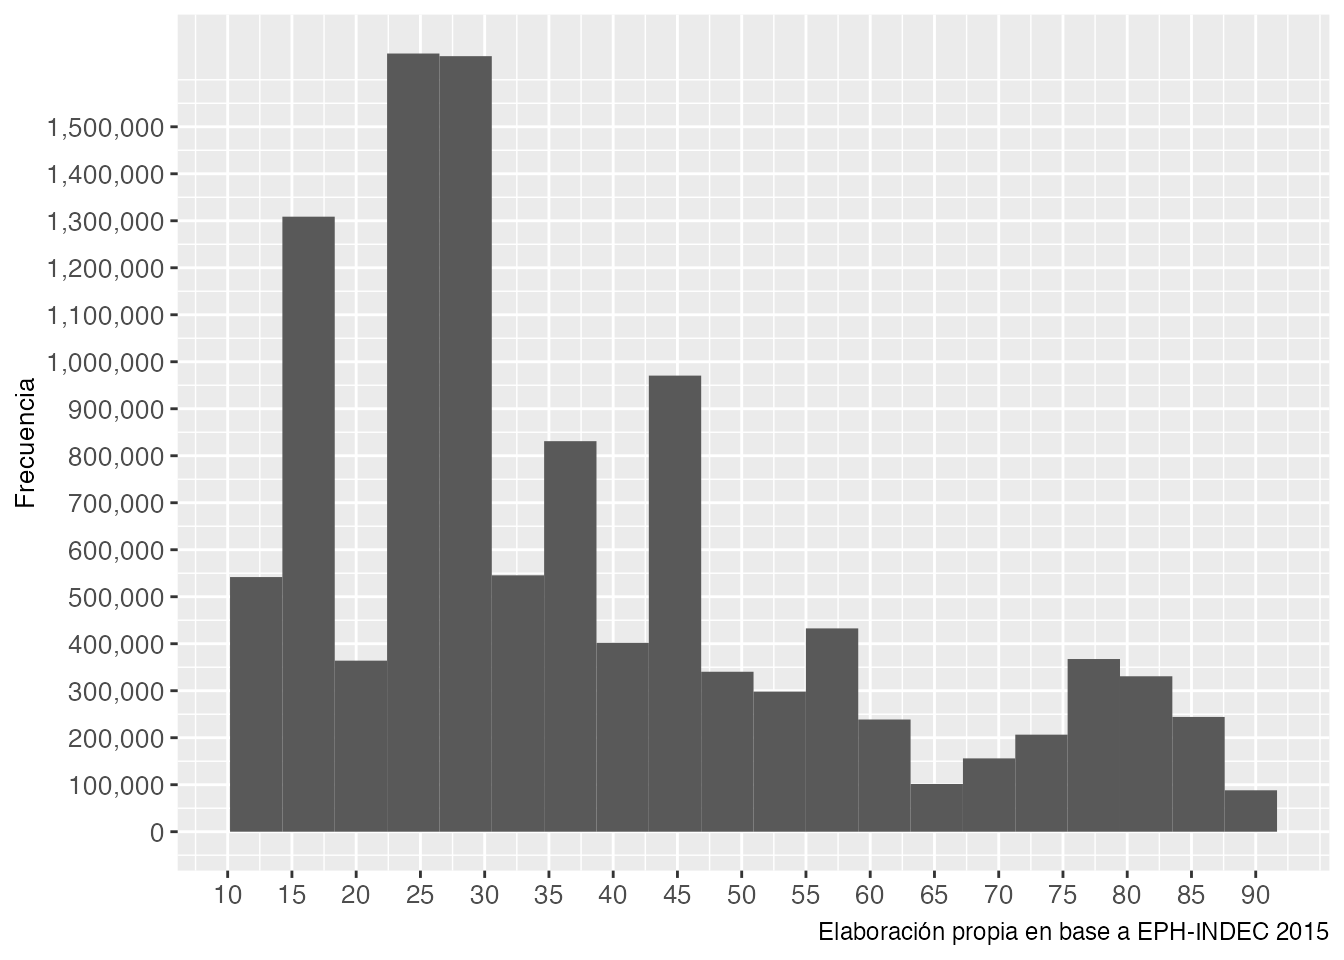
\includegraphics{docs_files/figure-latex/isei2-1} 

}

\caption{Histograma de frecuencias la escala ISEI}\label{fig:isei2}
\end{figure}

El histograma nos muestra donde se concentran las personas según sus ocupaciones. De esta forma, la mayor parte de la población se encuentra entre el puntaje 15 y 43 de la escala. Por el contrario, las ocupaciones mejores puntadas tienen una menor proporción de personas.

\hypertarget{unidades}{%
\subsection{Unidades de análisis y clases sociales}\label{unidades}}

\hypertarget{breve-discusiuxf3n-teuxf3rica}{%
\subsubsection[Breve discusión teórica]{\texorpdfstring{Breve discusión teórica\footnote{Este apartado recupera algunos aspectos abordados en el capítulo 2 de Rodríguez de la Fuente (\protect\hyperlink{ref-RodriguezdelaFuente2020}{2020})}}{Breve discusión teórica}}\label{breve-discusiuxf3n-teuxf3rica}}

Una vez construido empíricamente nuestro esquema de clases, es importante definir el universo de análisis a considerar, desde el punto de vista de la pertenencia de clase. Si bien está decisión es importante realizarla en etapas previas de la investigación, nos referimos a la importancia en la resolución metodológica de dicha cuestión. Hay varias formas de proceder, pero digamos que en primer lugar, es necesario establecer si nuestra población objetivo serán individuos u hogares. En el primer caso, como señala Torrado (\protect\hyperlink{ref-Torrado1998d}{1998b, pp. 236--237}), sería necesario considerar a la PEA, mientras que en el segundo caso a algún indicador del hogar como puede ser la posición del jefe/a activo/a de los hogares particulares.

La primera de estas opciones tiene la ventaja que permite una imagen más fiel de las características del sistema productivo al cual se está haciendo referencia, aunque sólo abarca a una población pequeña de la población. La consideración de los hogares, implica en este sentido, un aumento en la población analizada (por ejemplo, todos los hogares con jefe/a activo/a), a la vez que permite una mejor captación del conocimiento de la estructura social respecto a la medición de las condiciones de vida y comportamientos diversos, que únicamente pueden ser atribuidos a la esfera del hogar (\protect\hyperlink{ref-Torrado1998d}{Torrado, 1998b, p. 238}). En este sentido, cada unidad de análisis nos permiten observar fenómenos distintos de la realidad social y es decisión de los investigadores que camino seguir en función de los objetivos propuestos.

Un segundo aspecto a considerar es, parafraseando a Crompton (\protect\hyperlink{ref-Crompton2008}{2008, p. 124}), ``el problema de las mujeres''. Tanto al considerar como unidad de análisis a los individuos o a los hogares, los estudios de clases y movilidad social, han estado largamente dominados por enfoques que asignaban a las mujeres la misma posición que la del jefe de familia. Más allá de la larga discusión que abarcó gran parte de los años 80 y que mantiene sus repercusiones en la actualidad (\protect\hyperlink{ref-GomezRojas2011}{Gómez Rojas, 2011}; \protect\hyperlink{ref-Riveiro2017}{Riveiro, 2017}), resulta totalmente sesgado tanto teórico como metodológicamente la subsunción de las situaciones de las mujeres a la de los varones.

En este sentido, en forma resumida, cuatro enfoques se encuentran fundamentalmente en la bibliografía del análisis de clase para solucionar esta problemática (\protect\hyperlink{ref-FeitoAlonso1995b}{Feito Alonso, 1995b}). En primer lugar, puede citarse el enfoque \textbf{tradicional}, defendido en un primer momento por Goldthorpe (\protect\hyperlink{ref-Goldthorpe1983}{1983}), que sostiene que los hogares deben ser considerados como unidad de análisis, aunque debe ser la posición del varón jefe de familia quien le otorgue al grupo su posición de clase. En un segundo lugar podemos señalar el enfoque de \textbf{dominancia}, propuesto por Erikson (\protect\hyperlink{ref-Erikson1984}{1984}), que se basa en la determinación de la posición de clase del hogar a partir de la situación de clase del cónyuge cuya inserción sea más decisiva de cara a la determinación de intereses, patrones de consumo, condiciones de vivienda, etc. En términos simplificados, dicho enfoque, deriva la condición de clase del hogar de la posición mejor situada entre los cónyuges. Un tercer enfoque considera conjuntamente a la \textbf{posición de ambos cónyuges} para caracterizar al hogar. De lo que se trata es de generar una tipología de hogares que clasifique a los mismos en función de su carácter homogéneo (ambos cónyuges pertenecen a la misma clase) y heterogéneo (ambos cónyuges pertenecen a clases distintas). Dicho enfoque es subsidiario, principalmente, de la propuesta de Wright (\protect\hyperlink{ref-Wright1992}{1992}) al considerar las posiciones contradictorias (mediatas e inmediatas) dentro de la estructura de clases. Finalmente, un cuarto enfoque plantea la necesidad de considerar las posiciones de los \textbf{varones y mujeres de forma individual}, a partir de su propia situación de clase y sin tomar al hogar como unidad de análisis.

\hypertarget{opciones-metodoluxf3gicas}{%
\subsubsection{Opciones metodológicas}\label{opciones-metodoluxf3gicas}}

En esta sección vamos a explorar tres formas de abordar la estructura de clases a partir de la selección de distintas unidades de análisis: considerando a la \textbf{población ocupada}, considerando al hogar a través de la \textbf{jefatura} y considerando al hogar a través de la \textbf{dominancia}. Como señalamos, esta selección no es exhaustiva ni superadora. La elección de cada uno de los abordajes dependera de decisiones teórico-metodológicas.

En el primer caso, para considerar al universo de estudio de la población ocupada sólo necesitaremos filtrar nuestra base únicamente seleccionando a aquellos individuos que para la variable \textbf{ESTADO} se encuentran en condición de ocupados (1).

\begin{Shaded}
\begin{Highlighting}[]
\NormalTok{base\_PO }\OtherTok{\textless{}{-}}\NormalTok{ eph\_ind\_215 }\SpecialCharTok{\%\textgreater{}\%}
    \FunctionTok{filter}\NormalTok{(ESTADO }\SpecialCharTok{==} \DecValTok{1}\NormalTok{)  }\CommentTok{\# Creamos una nueva base con el filtro de la población ocupada}

\NormalTok{summarytools}\SpecialCharTok{::}\FunctionTok{freq}\NormalTok{(base\_PO}\SpecialCharTok{$}\NormalTok{clase6\_factor, }\AttributeTok{weights =}\NormalTok{ base\_PO}\SpecialCharTok{$}\NormalTok{PONDERA, }\AttributeTok{justify =} \StringTok{"center"}\NormalTok{,}
    \AttributeTok{cumul =} \ConstantTok{FALSE}\NormalTok{)}
\end{Highlighting}
\end{Shaded}

\begin{verbatim}
Weighted Frequencies  
base_PO$clase6_factor  
Type: Factor  
Weights: PONDERA  

                                                 Freq       % Valid   % Total 
-------------------------------------------- ------------- --------- ---------
                 Clase alta                    49429.00      0.45      0.44   
           Clase media - autónoma             1446840.00     13.07     12.99  
          Clase media - asalariada            4095309.00     36.98     36.77  
          Clase obrera - autónoma             1013705.00     9.15      9.10   
         Clase obrera - asalariada            3708848.00     33.49     33.30  
   Clase obrera - trabajadores marginales      758822.00     6.85      6.81   
                    <NA>                       63766.00                0.57   
                   Total                      11136719.00   100.00    100.00  
\end{verbatim}

De esta forma, observamos que la población ocupada asciende a \texttt{11.136.719}, considerando \texttt{63.766} valores perdidos, es decir, personas que no pudieron ser clasificadas bajo esquema empleado. Esta tabla nos brindaría una imagen de cómo que conforma la estructura de clases en la población ocupada.

Si en cambio lo que queremos observar es al universo de los hogares, utilizaremos las características económicas-laborales de uno de los miembros del hogar para caracterizar a toda la unidad. En el primer caso, nos basaremos en la \textbf{jefatura del hogar}. Para ello, filtraremos aquellos casos que sean jefe/a (1) en la variable \textbf{CH03}.

\begin{Shaded}
\begin{Highlighting}[]
\NormalTok{base\_jefatura }\OtherTok{\textless{}{-}}\NormalTok{ eph\_ind\_215 }\SpecialCharTok{\%\textgreater{}\%}
    \FunctionTok{filter}\NormalTok{(CH03 }\SpecialCharTok{==} \DecValTok{1}\NormalTok{)  }\CommentTok{\# Nos quedamos únicamente con los/las jefe/as de hogar}

\NormalTok{summarytools}\SpecialCharTok{::}\FunctionTok{freq}\NormalTok{(base\_jefatura}\SpecialCharTok{$}\NormalTok{clase6\_factor, }\AttributeTok{weights =}\NormalTok{ base\_jefatura}\SpecialCharTok{$}\NormalTok{PONDERA,}
    \AttributeTok{justify =} \StringTok{"center"}\NormalTok{, }\AttributeTok{cumul =} \ConstantTok{FALSE}\NormalTok{)}
\end{Highlighting}
\end{Shaded}

\begin{verbatim}
Weighted Frequencies  
base_jefatura$clase6_factor  
Type: Factor  
Weights: PONDERA  

                                                 Freq      % Valid   % Total 
-------------------------------------------- ------------ --------- ---------
                 Clase alta                    28725.00     0.51      0.34   
           Clase media - autónoma             792515.00     14.09     9.42   
          Clase media - asalariada            1922384.00    34.19     22.84  
          Clase obrera - autónoma             618087.00     10.99     7.34   
         Clase obrera - asalariada            1941096.00    34.52     23.06  
   Clase obrera - trabajadores marginales     320537.00     5.70      3.81   
                    <NA>                      2792656.00              33.18  
                   Total                      8416000.00   100.00    100.00  
\end{verbatim}

Si comparamos con la tabla anterior, los valores han cambiado. Esto se debe a que pasamos de \emph{considerar} individuos a considerar \emph{hogares}. El número total de hogares es de \texttt{8.416.000} y los casos perdidos ascienden a \texttt{2.792.656}, grupo conformado por hogares con jefatura desocupada o inactiva.

Finalmente podemos considerar el enfoque de \textbf{dominancia}. Este es algo más complejo en su elaboración, ya que es necesario aplicar una serie de pasos. De este modo, definimos a la posición de clase social del hogar como aquella ocupada por el cónyuge que posee la posición más aventajada. En los casos de hogares no nucleares o con el núcleo incompleto (ausencia de uno de los cónyuges), se tomará directamente la clase del jefe/a.

\begin{Shaded}
\begin{Highlighting}[]
\CommentTok{\# 1) Selecciono solo a jefe/as y cónyuges}
\NormalTok{base\_dominancia }\OtherTok{\textless{}{-}}\NormalTok{ eph\_ind\_215 }\SpecialCharTok{\%\textgreater{}\%} 
  \FunctionTok{filter}\NormalTok{(CH03 }\SpecialCharTok{==} \DecValTok{1} \SpecialCharTok{|}\NormalTok{ CH03 }\SpecialCharTok{==} \DecValTok{2}\NormalTok{)}

\CommentTok{\# 2) Agrupando por vivienda (CODUSU) y hogar (NRO\_HOGAR), creo una nueva variable que compute cual es la posición de clase más alta, que este caso es el valor más bajo (min), ya que las clases se ordenan de menor a mayor en las variables.}
\NormalTok{base\_dominancia }\OtherTok{\textless{}{-}}\NormalTok{ base\_dominancia }\SpecialCharTok{\%\textgreater{}\%} 
  \FunctionTok{group\_by}\NormalTok{(CODUSU, NRO\_HOGAR) }\SpecialCharTok{\%\textgreater{}\%} 
  \FunctionTok{mutate}\NormalTok{(}\AttributeTok{clase\_dom =} \FunctionTok{min}\NormalTok{(clase6, }\AttributeTok{na.rm =} \ConstantTok{TRUE}\NormalTok{)) }

\CommentTok{\# 3) Identifico qué cónyuge es el dominante. }
\NormalTok{base\_dominancia }\OtherTok{\textless{}{-}}\NormalTok{ base\_dominancia }\SpecialCharTok{\%\textgreater{}\%} 
  \FunctionTok{mutate}\NormalTok{(}\AttributeTok{dom =} \FunctionTok{case\_when}\NormalTok{(clase6 }\SpecialCharTok{==}\NormalTok{ clase\_dom }\SpecialCharTok{\textasciitilde{}} \DecValTok{1}\NormalTok{, }\CommentTok{\# dominante}
\NormalTok{                         clase6 }\SpecialCharTok{\textgreater{}}\NormalTok{ clase\_dom }\SpecialCharTok{\textasciitilde{}} \DecValTok{0}\NormalTok{)) }\CommentTok{\# no dominante}

\CommentTok{\# 4) Identifico a los hogares en el que los cónyuges comparten la dominancia, es decir, tienen la misma clase. Para eso sumo (dom\_sum) dentro del hogar la variable "dom". Luego a partir de ese resultado puedo definir quien es el miembro dominante y otorgar la dominancia al jefe/a en el caso que ambos tengan la misma clase.}
\NormalTok{base\_dominancia }\OtherTok{\textless{}{-}}\NormalTok{  base\_dominancia }\SpecialCharTok{\%\textgreater{}\%} 
  \FunctionTok{group\_by}\NormalTok{(CODUSU, NRO\_HOGAR) }\SpecialCharTok{\%\textgreater{}\%} 
  \FunctionTok{mutate}\NormalTok{(}\AttributeTok{dom\_sum =} \FunctionTok{sum}\NormalTok{(dom, }\AttributeTok{na.rm =} \ConstantTok{TRUE}\NormalTok{))}

\NormalTok{base\_dominancia }\OtherTok{\textless{}{-}}\NormalTok{ base\_dominancia }\SpecialCharTok{\%\textgreater{}\%} 
  \FunctionTok{mutate}\NormalTok{(}\AttributeTok{dominancia =} \FunctionTok{case\_when}\NormalTok{(dom }\SpecialCharTok{==} \DecValTok{1} \SpecialCharTok{\&}\NormalTok{ dom\_sum }\SpecialCharTok{==} \DecValTok{1} \SpecialCharTok{\textasciitilde{}} \DecValTok{1}\NormalTok{, }\CommentTok{\#dominante}
\NormalTok{                         dom }\SpecialCharTok{==} \DecValTok{0} \SpecialCharTok{\&}\NormalTok{ dom\_sum }\SpecialCharTok{==} \DecValTok{1} \SpecialCharTok{\textasciitilde{}} \DecValTok{0}\NormalTok{, }\CommentTok{\# no dominante}
\NormalTok{                         dom }\SpecialCharTok{==} \DecValTok{1} \SpecialCharTok{\&}\NormalTok{ dom\_sum }\SpecialCharTok{==} \DecValTok{2} \SpecialCharTok{\&}\NormalTok{ CH03 }\SpecialCharTok{==} \DecValTok{1} \SpecialCharTok{\textasciitilde{}} \DecValTok{1}\NormalTok{, }\CommentTok{\# dominante por ser jefe de hogar}
\NormalTok{                         dom }\SpecialCharTok{==} \DecValTok{1} \SpecialCharTok{\&}\NormalTok{ dom\_sum }\SpecialCharTok{==} \DecValTok{2} \SpecialCharTok{\&}\NormalTok{ CH03 }\SpecialCharTok{==} \DecValTok{2} \SpecialCharTok{\textasciitilde{}} \DecValTok{0}\NormalTok{)) }\CommentTok{\# no dominante por no ser jefe de hogar}

\CommentTok{\# 5) Filtro la base con los "dominantes" y borro las variables intermedias que cree.}
\NormalTok{base\_dominancia }\OtherTok{\textless{}{-}}\NormalTok{ base\_dominancia }\SpecialCharTok{\%\textgreater{}\%} 
  \FunctionTok{filter}\NormalTok{(dominancia }\SpecialCharTok{==} \DecValTok{1}\NormalTok{)}

\NormalTok{base\_dominancia}\SpecialCharTok{$}\NormalTok{dom }\OtherTok{\textless{}{-}} \ConstantTok{NULL}
\NormalTok{base\_dominancia}\SpecialCharTok{$}\NormalTok{dom\_sum }\OtherTok{\textless{}{-}} \ConstantTok{NULL}

\NormalTok{summarytools}\SpecialCharTok{::}\FunctionTok{freq}\NormalTok{(base\_dominancia}\SpecialCharTok{$}\NormalTok{clase6\_factor, }\AttributeTok{weights =}\NormalTok{ base\_dominancia}\SpecialCharTok{$}\NormalTok{PONDERA, }\AttributeTok{justify =} \StringTok{"center"}\NormalTok{, }\AttributeTok{cumul =} \ConstantTok{FALSE}\NormalTok{)}
\end{Highlighting}
\end{Shaded}

\begin{verbatim}
Weighted Frequencies  
base_dominancia$clase6_factor  
Type: Factor  
Weights: PONDERA  

                                                 Freq      % Valid   % Total 
-------------------------------------------- ------------ --------- ---------
                 Clase alta                    45732.00     0.75      0.75   
           Clase media - autónoma             1027302.00    16.95     16.95  
          Clase media - asalariada            2229496.00    36.80     36.80  
          Clase obrera - autónoma             621547.00     10.26     10.26  
         Clase obrera - asalariada            1831160.00    30.22     30.22  
   Clase obrera - trabajadores marginales     303996.00     5.02      5.02   
                    <NA>                         0.00                 0.00   
                   Total                      6059233.00   100.00    100.00  
\end{verbatim}

En este caso, luego de aplicar las transformaciones, contamos con \texttt{6.059.233} hogares clasificados a partir de la posición dominante de uno de lo cónyuges.

\hypertarget{part-anuxe1lisis}{%
\part{Análisis}\label{part-anuxe1lisis}}

\hypertarget{independiente}{%
\section{La clase como variable independiente}\label{independiente}}

Este capítulo tiene como propósito presentar a las clases sociales como uno de los factores estructuradores de la desigualdad social. Una vez ya revisadas las teorías que explican el modo en el que la sociedades pueden dividirse en clases, y a la vez, ser operacionalizadas para su estudio empírico a través de fuentes de datos, por un lado indagamos acerca del rol que presenta el sistema de clases en la configuración de diversos tipos de desigualdades y resultados atribuibles a individuos y hogares. Para ello exploraremos algunas teorías que han intentado explicar el vínculo entre dichos aspectos. Por el otro, indagaremos algunas de las dimensiones más relevadas (ingresos, hábitat, demografía) y presentaremos diversas formas de explorar la relación entre las variables.\\
Las siguientes preguntas guiarán al capítulo:\\
- ¿Sobre qué aspectos la estructura de clases resulta un factor explicativo?\\
- ¿Qué elementos teóricos permiten explicar el papel de la estructura de clases como factor condicionante de la clase social?\\
- ¿Cuáles son las principales dimensiones relevadas por los investigadores en el análisis de clases?\\
- ¿Qué técnicas exploratorias podemos utilizar para presentar los resultados?\\
- ¿Qué rol juegan otros factores explicativos de la desigualdad y cómo pueden ser estudiados en conjunto con las clases sociales?

Al completar el capítulo se espera que los lectores puedan:

\begin{enumerate}
\def\labelenumi{\arabic{enumi}.}
\tightlist
\item
  Conocer los principales enfoque teóricos que postulan a las clases sociales como un aspecto clave para la comprensión de otras desigualdades sociales.\\
\item
  Revisar las principales dimensiones de la realidad que fueron estudiadas desde un enfoque de clases sociales.\\
\item
  Presentar los principales abordajes exploratorios y descriptivos que pueden realizarse teniendo a la clase social como variable independiente.\\
\item
  Introducir el enfoque multivariable en el estudio de la desigualdad social a partir del análisis de clase.
\end{enumerate}

Para una mayor comprensión del capítulo recomendamos la lectura de los siguientes textos:

\begin{itemize}
\item
  Dubet, F. (\protect\hyperlink{ref-Dubet2015}{2015}). Clases sociales y descripción de la sociedad. Revista Ensambles, (3).
\item
  Torrado, S. (\protect\hyperlink{ref-Torrado1995}{1995}). Vivir apurado para morirse joven: Reflexiones sobre la transferencia intergeneracional de la pobreza. Revista Sociedad, 7.
\item
  Maceira, V. (\protect\hyperlink{ref-Maceira2018}{2018}). Clases y diferenciación social. En J. I. Piovani y A. Salvia (Eds.), La Argentina en el siglo XXI. Cómo somos, vivimos y convivimos en una sociedad desigual. Encuesta Nacional sobre la Estructura Social. Buenos Aires: Siglo Veintiuno Editores. (\textbf{Revisa varios aspectos: autopercepción de clase, condiciones laborales, movilidad social, demografía del hogar})
\item
  Pla, J., Rodríguez de la Fuente, J., y Sacco, N. (\protect\hyperlink{ref-Pla.etal2018}{2018}). Clases sociales y condiciones de vida en el Gran Buenos Aires (2003-2013). Revista Colombiana de Sociología, 41(2), 189-231. (\textbf{Análisis de ingresos condiciones laborales y habitacionales})
\item
  Sacco, N., y Borges, G. (\protect\hyperlink{ref-Sacco2018}{2018}). ¿Converge la fecundidad en Brasil y Argentina? Un enfoque desde las desigualdades. Revista Brasileira de Estudos de População, 35(1), 1-29. (\textbf{Análisis demográfico})
\item
  Solís, P., Chávez Molina, E., y Cobos, D. (\protect\hyperlink{ref-Solis.etal2019}{2019}). Class Structure, Labor Market Heterogeneity, and Living Conditions in Latin America. Latin American Research Review, 54(4). (\textbf{Análisis comparativo en Latinoamérica sobre ingresos y condiciones laborales})
\item
  Elbert, R. (\protect\hyperlink{ref-Elbert2020}{2020}). Posición de clase objetiva y auto-identificación de clase. En P. Dalle, R. Sautu, P. Boniolo, y R. Elbert, El análisis de clases sociales. Pensando la movilidad social, la residencia, los lazos sociales, la identidad y la agencia. Buenos Aires: CLACSO - IIGG. (\textbf{Autopercepción de clase})
\end{itemize}

\hypertarget{huevo}{%
\subsection{La estructura de clases ¿el huevo o la gallina?}\label{huevo}}

Para entender a qué nos referimos al conceptualizar a la clase social como variable independiente podemos pensar en el típico ejemplo de qué viene primero, si el huevo o la gallina. En este caso, la estructura de clases tiene potencial tanto de explicación como de fenómeno a ser explicado. En esta característica radican su versatilidad y complejidad. Lo cierto es que en esta sección, abordaremos de qué manera puede influir la clase en diversos aspectos de la desigualdad social, inherente a las sociedades actuales.

Dicho en otros términos, si tomamos un modelo simple, podemos representar a la variable independiente como X y a la variable dependiente como Y, veremos que:

X ---\textgreater{} Y

Esta simplificación de la realidad nos brinda un modo sencillo de analizar la forma en que se relacionan las variables, dado que es la clase aquella que influye o afecta (pero nunca determina) a la desigualdad social. Asimismo, nuestra \texttt{Y} podría representar a múltiples factores o fenómenos que varían según el comportamiento de \texttt{X}. Esto es, por ejemplo, el modo en que la estructura de clases tiene efectos sobre la distribución de los ingresos de los individuos y de los hogares, o bien en el hábitat, los fenómenos demográficos, las condiciones laborales, el consumo, el capital cultural, los factores psico-sociales, entre otros. En la literatura, estos \emph{resultados} ligados al posicionamiento de clase, fueron concebidos bajo diferentes ideas: ``oportunidades de vida'', ``condiciones de vida'', ``nivel de vida'', ``bienestar'', ``riqueza'', ``recursos'', ``activos'', ``capitales'', etc.

Con la finalidad de presentar estas numerosas relaciones que la variable \emph{clase} posee en los fenómenos aquí presentados, tendremos en cuanta una a una las diferentes perspectivas que nos permiten comprender cada una de ellas.

\hypertarget{el-enfoque-relacional-weberiano}{%
\subsubsection{El enfoque relacional-weberiano}\label{el-enfoque-relacional-weberiano}}

La literatura destaca la relación existente entre las \textbf{clases} y las \textbf{oportunidades de vida}. Dicho de otro modo, existe una relación entre la estructura en la que se ubican los individuos y la posibilidad de lograr o alcanzar ciertas oportunidades de vida. Entonces, como señala Benza (\protect\hyperlink{ref-Benza2014}{2014}), esto no significa que las clases determinen necesariamente, o generen directamente tales o cuáles ``chances'' de vida de las personas, sino más bien, contribuyen a la probabilidad de que se den. En pocas palabras, pertenecer a una clase hace que sea mayormente posible el hecho de lograr determinadas oportunidades de vida, que en el caso de pertenecer a otra posición de la estructura social serían diferentes.

Ya presentadas las diferencias que se ven afectadas por la pertenencia a una clase u otra, es decir, las diferencias entre clases, ahora nos centramos en ver qué sucede dentro de las clases, o sea, al interior de un grupo de la estructura social. Para ello, recordamos el argumento de Breen (\protect\hyperlink{ref-Breen2005}{2005, p. 3}) acerca de la variabilidad en las oportunidades de vida que existen entre los miembros de una misma clase. Estas se deben a que las clases dependen de múltiples factores, lo que hace que cierta posición de clase no se corresponda totalmente ---como condición \emph{sine qua non}--- con determinado conjunto de oportunidades de vida. La relación es más bien explicada como a consiguiente: las oportunidades de vida no se estructuran únicamente por la estructura de clases. También intervienen otros factores relevantes como la edad, el género, la etnia, el lugar de nacimiento y/o el nivel educativo.

¿Cómo funcionan, entonces, las oportunidades de vida? Estas se componen de una amplia paleta de aspectos tales como los ingresos, la capacidad de ahorro, la seguridad económica, la estabilidad económica, las expectativas económicas, la salud, entre otros (\protect\hyperlink{ref-Chan.Goldthorpe2007}{Chan \& Goldthorpe, 2007}; \protect\hyperlink{ref-Goldthorpe.McKnight2006}{J. H. Goldthorpe \& McKnight, 2006}). De este modo, explorar la relación entre la estructura de clases y las oportunidades de vida, implica tomar como punto de partida a las clases para analizar cómo afectan a los fenómenos de tinte cuantitativo (por ejemplo: la distribución del ingreso), y aquellos de tipo cualitativo (por ejemplo: expectativas económicas). Siguiendo esta línea de acercamiento relacional, vemos que para Goldthorpe las clases sociales deben pensarse no en términos jerárquicos (respecto a los resultados y oportunidades a los cuales se asocian) sino en términos de posiciones más o menos ventajosas.

\hypertarget{estructural-funcionalismo}{%
\subsubsection{Estructural funcionalismo}\label{estructural-funcionalismo}}

Hablar del \textbf{estructural funcionalismo} implica ``movernos'' en el nivel de abstracción del análisis. Si el enfoque weberiano nos permite ahondar en los aspectos macro estructurales, el funcionalismo hace foco en el nivel intermedio o meso de análisis sociológico. Desde esta perspectiva, partiendo de criterios evaluatorios, el sistema social jerarquiza a las posiciones en función del mérito y la especificidad de la ocupación detentada y también establece el ``paquete de recompensas'' (\protect\hyperlink{ref-CachonRodriguez1989}{Cachón Rodríguez, 1989}; \protect\hyperlink{ref-Parsons1954}{Parsons, 1954}). Esto es, la correspondencia ordenada e institucionalizada de la relación estratificación-recompensas.

Como consecuencia, lejos de referirse a la estratificación social como un factor estructurador de las desigualdades, las recompensas deben pesarse como una consecuencia del proceso de igualdad de oportunidades, es decir, una ``desigualdad institucionalizada'' de resultados existentes.

\hypertarget{un-enfoque-intermedio}{%
\subsubsection{Un enfoque intermedio}\label{un-enfoque-intermedio}}

En un camino intermedio de estos dos enfoques se encuentra la propuesta de Grusky (\protect\hyperlink{ref-Grusky2008}{2008}). El autor plantea que existen tres componentes clave que definen a un sistema de estratificación: 1) los procesos institucionales que definen qué tipos de bienes deben ser valorados y deseables; 2) las reglas de asignación que distribuyen dichos bienes según ocupaciones en la división del trabajo y 3) los procesos de movilidad que ligan a los individuos con las ocupaciones y brindan un control desigual sobre los recursos valorados (\protect\hyperlink{ref-Grusky2008}{Grusky, 2008, p. 5}), ilustrado en la \ref{tab:grusky}.

Dentro de los activos que se encuentran desigualmente distribuidos en la sociedad, podemos nombrar a los: económicos, de poder, culturales, religiosos, sociales, honoríficos, civiles, humanos y físicos.

\global\setlength{\Oldarrayrulewidth}{\arrayrulewidth}

\global\setlength{\Oldtabcolsep}{\tabcolsep}

\setlength{\tabcolsep}{0pt}

\renewcommand*{\arraystretch}{1.5}



\providecommand{\ascline}[3]{\noalign{\global\arrayrulewidth #1}\arrayrulecolor[HTML]{#2}\cline{#3}}

\begin{longtable}[c]{cccc}

\caption{Tipos\ de\ activos\ y\ ejemplos\ de\ grupos\ aventajados\ y\ desaventajados}\label{tab:grusky}\\

\ascline{1.5pt}{666666}{1-4}

\multicolumn{2}{>{}c}{\textcolor[HTML]{000000}{\fontsize{10}{10}\selectfont{\textbf{Activos}}}} & \multicolumn{2}{>{}c}{\textcolor[HTML]{000000}{\fontsize{10}{10}\selectfont{\textbf{Ejemplos}}}} \\

\ascline{1.5pt}{666666}{1-4}\endfirsthead \caption[]{Tipos\ de\ activos\ y\ ejemplos\ de\ grupos\ aventajados\ y\ desaventajados}\label{tab:grusky}\\

\ascline{1.5pt}{666666}{1-4}

\multicolumn{2}{>{}c}{\textcolor[HTML]{000000}{\fontsize{10}{10}\selectfont{\textbf{Activos}}}} & \multicolumn{2}{>{}c}{\textcolor[HTML]{000000}{\fontsize{10}{10}\selectfont{\textbf{Ejemplos}}}} \\

\ascline{1.5pt}{666666}{1-4}\endhead



\multicolumn{4}{>{}l}{\textcolor[HTML]{000000}{\fontsize{10}{10}\selectfont{Fuente:\ Grusky\ (2008)}}} \\

\endfoot



\multicolumn{1}{>{}c}{\textcolor[HTML]{000000}{\fontsize{10}{10}\selectfont{\textit{Tipo\ de\ activos}}}} & \multicolumn{1}{>{}c}{\textcolor[HTML]{000000}{\fontsize{10}{10}\selectfont{\textit{Ejemplos}}}} & \multicolumn{1}{>{}c}{\textcolor[HTML]{000000}{\fontsize{10}{10}\selectfont{\textit{Aventajados}}}} & \multicolumn{1}{>{}c}{\textcolor[HTML]{000000}{\fontsize{10}{10}\selectfont{\textit{Desaventajados}}}} \\

\ascline{1pt}{000000}{1-4}



\multicolumn{1}{>{}c}{\textcolor[HTML]{000000}{\fontsize{10}{10}\selectfont{Económico}}} & \multicolumn{1}{>{}c}{\textcolor[HTML]{000000}{\fontsize{10}{10}\selectfont{Riqueza}}} & \multicolumn{1}{>{}c}{\textcolor[HTML]{000000}{\fontsize{10}{10}\selectfont{Billonarios}}} & \multicolumn{1}{>{}c}{\textcolor[HTML]{000000}{\fontsize{10}{10}\selectfont{Trabajador\ quebrado}}} \\





\multicolumn{1}{>{}c}{\textcolor[HTML]{000000}{\fontsize{10}{10}\selectfont{}}} & \multicolumn{1}{>{}c}{\textcolor[HTML]{000000}{\fontsize{10}{10}\selectfont{Ingresos}}} & \multicolumn{1}{>{}c}{\textcolor[HTML]{000000}{\fontsize{10}{10}\selectfont{Profesionales}}} & \multicolumn{1}{>{}c}{\textcolor[HTML]{000000}{\fontsize{10}{10}\selectfont{Obrero}}} \\





\multicolumn{1}{>{}c}{\textcolor[HTML]{000000}{\fontsize{10}{10}\selectfont{}}} & \multicolumn{1}{>{}c}{\textcolor[HTML]{000000}{\fontsize{10}{10}\selectfont{Propiedad}}} & \multicolumn{1}{>{}c}{\textcolor[HTML]{000000}{\fontsize{10}{10}\selectfont{Capitalistas}}} & \multicolumn{1}{>{}c}{\textcolor[HTML]{000000}{\fontsize{10}{10}\selectfont{Empleado}}} \\





\multicolumn{1}{>{}c}{\textcolor[HTML]{000000}{\fontsize{10}{10}\selectfont{Poder}}} & \multicolumn{1}{>{}c}{\textcolor[HTML]{000000}{\fontsize{10}{10}\selectfont{Poder\ político}}} & \multicolumn{1}{>{}c}{\textcolor[HTML]{000000}{\fontsize{10}{10}\selectfont{Primer\ ministro}}} & \multicolumn{1}{>{}c}{\textcolor[HTML]{000000}{\fontsize{10}{10}\selectfont{Persona\ sin\ derechos}}} \\





\multicolumn{1}{>{}c}{\textcolor[HTML]{000000}{\fontsize{10}{10}\selectfont{}}} & \multicolumn{1}{>{}c}{\textcolor[HTML]{000000}{\fontsize{10}{10}\selectfont{Autoridad\ en\ el\ trabajo}}} & \multicolumn{1}{>{}c}{\textcolor[HTML]{000000}{\fontsize{10}{10}\selectfont{Manager}}} & \multicolumn{1}{>{}c}{\textcolor[HTML]{000000}{\fontsize{10}{10}\selectfont{Trabajador\ subordinado}}} \\





\multicolumn{1}{>{}c}{\textcolor[HTML]{000000}{\fontsize{10}{10}\selectfont{}}} & \multicolumn{1}{>{}c}{\textcolor[HTML]{000000}{\fontsize{10}{10}\selectfont{Autoridad\ en\ el\ hogar}}} & \multicolumn{1}{>{}c}{\textcolor[HTML]{000000}{\fontsize{10}{10}\selectfont{Jefe/a\ de\ hogar}}} & \multicolumn{1}{>{}c}{\textcolor[HTML]{000000}{\fontsize{10}{10}\selectfont{Niño}}} \\





\multicolumn{1}{>{}c}{\textcolor[HTML]{000000}{\fontsize{10}{10}\selectfont{Cultural}}} & \multicolumn{1}{>{}c}{\textcolor[HTML]{000000}{\fontsize{10}{10}\selectfont{Conocimiento}}} & \multicolumn{1}{>{}c}{\textcolor[HTML]{000000}{\fontsize{10}{10}\selectfont{Intelectuales}}} & \multicolumn{1}{>{}c}{\textcolor[HTML]{000000}{\fontsize{10}{10}\selectfont{Persona\ sin\ educación}}} \\





\multicolumn{1}{>{}c}{\textcolor[HTML]{000000}{\fontsize{10}{10}\selectfont{}}} & \multicolumn{1}{>{}c}{\textcolor[HTML]{000000}{\fontsize{10}{10}\selectfont{Cultura\ digital}}} & \multicolumn{1}{>{}c}{\textcolor[HTML]{000000}{\fontsize{10}{10}\selectfont{Residentes\ de\ Sillicon\ Valley}}} & \multicolumn{1}{>{}c}{\textcolor[HTML]{000000}{\fontsize{10}{10}\selectfont{Residente\ de\ otros\ lugares}}} \\





\multicolumn{1}{>{}c}{\textcolor[HTML]{000000}{\fontsize{10}{10}\selectfont{}}} & \multicolumn{1}{>{}c}{\textcolor[HTML]{000000}{\fontsize{10}{10}\selectfont{Buenas\ maneras}}} & \multicolumn{1}{>{}c}{\textcolor[HTML]{000000}{\fontsize{10}{10}\selectfont{Aristocracia}}} & \multicolumn{1}{>{}c}{\textcolor[HTML]{000000}{\fontsize{10}{10}\selectfont{Plebeyos}}} \\





\multicolumn{1}{>{}c}{\textcolor[HTML]{000000}{\fontsize{10}{10}\selectfont{Social}}} & \multicolumn{1}{>{}c}{\textcolor[HTML]{000000}{\fontsize{10}{10}\selectfont{Club\ sociales}}} & \multicolumn{1}{>{}c}{\textcolor[HTML]{000000}{\fontsize{10}{10}\selectfont{Miembro\ de\ un\ club\ de\ campo}}} & \multicolumn{1}{>{}c}{\textcolor[HTML]{000000}{\fontsize{10}{10}\selectfont{No\ miembro}}} \\





\multicolumn{1}{>{}c}{\textcolor[HTML]{000000}{\fontsize{10}{10}\selectfont{}}} & \multicolumn{1}{>{}c}{\textcolor[HTML]{000000}{\fontsize{10}{10}\selectfont{Asociaciones\ profesionales}}} & \multicolumn{1}{>{}c}{\textcolor[HTML]{000000}{\fontsize{10}{10}\selectfont{Miembro\ de\ sindicato}}} & \multicolumn{1}{>{}c}{\textcolor[HTML]{000000}{\fontsize{10}{10}\selectfont{No\ miembro}}} \\





\multicolumn{1}{>{}c}{\textcolor[HTML]{000000}{\fontsize{10}{10}\selectfont{}}} & \multicolumn{1}{>{}c}{\textcolor[HTML]{000000}{\fontsize{10}{10}\selectfont{Redes\ informales}}} & \multicolumn{1}{>{}c}{\textcolor[HTML]{000000}{\fontsize{10}{10}\selectfont{Washington\ A-List}}} & \multicolumn{1}{>{}c}{\textcolor[HTML]{000000}{\fontsize{10}{10}\selectfont{Desconocido}}} \\





\multicolumn{1}{>{}c}{\textcolor[HTML]{000000}{\fontsize{10}{10}\selectfont{Honorífico}}} & \multicolumn{1}{>{}c}{\textcolor[HTML]{000000}{\fontsize{10}{10}\selectfont{Ocupacional}}} & \multicolumn{1}{>{}c}{\textcolor[HTML]{000000}{\fontsize{10}{10}\selectfont{Juez}}} & \multicolumn{1}{>{}c}{\textcolor[HTML]{000000}{\fontsize{10}{10}\selectfont{Recolector\ de\ residuos}}} \\





\multicolumn{1}{>{}c}{\textcolor[HTML]{000000}{\fontsize{10}{10}\selectfont{}}} & \multicolumn{1}{>{}c}{\textcolor[HTML]{000000}{\fontsize{10}{10}\selectfont{Religioso}}} & \multicolumn{1}{>{}c}{\textcolor[HTML]{000000}{\fontsize{10}{10}\selectfont{Santo}}} & \multicolumn{1}{>{}c}{\textcolor[HTML]{000000}{\fontsize{10}{10}\selectfont{Excomulgado}}} \\





\multicolumn{1}{>{}c}{\textcolor[HTML]{000000}{\fontsize{10}{10}\selectfont{}}} & \multicolumn{1}{>{}c}{\textcolor[HTML]{000000}{\fontsize{10}{10}\selectfont{Basado\ en\ el\ mérito}}} & \multicolumn{1}{>{}c}{\textcolor[HTML]{000000}{\fontsize{10}{10}\selectfont{Premio\ Nobel}}} & \multicolumn{1}{>{}c}{\textcolor[HTML]{000000}{\fontsize{10}{10}\selectfont{No\ ganador}}} \\





\multicolumn{1}{>{}c}{\textcolor[HTML]{000000}{\fontsize{10}{10}\selectfont{Civil}}} & \multicolumn{1}{>{}c}{\textcolor[HTML]{000000}{\fontsize{10}{10}\selectfont{Derecho\ al\ trabajo}}} & \multicolumn{1}{>{}c}{\textcolor[HTML]{000000}{\fontsize{10}{10}\selectfont{Ciudadano}}} & \multicolumn{1}{>{}c}{\textcolor[HTML]{000000}{\fontsize{10}{10}\selectfont{Migrante\ ilegal}}} \\





\multicolumn{1}{>{}c}{\textcolor[HTML]{000000}{\fontsize{10}{10}\selectfont{}}} & \multicolumn{1}{>{}c}{\textcolor[HTML]{000000}{\fontsize{10}{10}\selectfont{Debido\ proceso}}} & \multicolumn{1}{>{}c}{\textcolor[HTML]{000000}{\fontsize{10}{10}\selectfont{Ciudadano}}} & \multicolumn{1}{>{}c}{\textcolor[HTML]{000000}{\fontsize{10}{10}\selectfont{Supuesto\ terrorista}}} \\





\multicolumn{1}{>{}c}{\textcolor[HTML]{000000}{\fontsize{10}{10}\selectfont{}}} & \multicolumn{1}{>{}c}{\textcolor[HTML]{000000}{\fontsize{10}{10}\selectfont{Voto}}} & \multicolumn{1}{>{}c}{\textcolor[HTML]{000000}{\fontsize{10}{10}\selectfont{Ciudadano}}} & \multicolumn{1}{>{}c}{\textcolor[HTML]{000000}{\fontsize{10}{10}\selectfont{Delincuente}}} \\





\multicolumn{1}{>{}c}{\textcolor[HTML]{000000}{\fontsize{10}{10}\selectfont{Humano}}} & \multicolumn{1}{>{}c}{\textcolor[HTML]{000000}{\fontsize{10}{10}\selectfont{Formación\ laboral}}} & \multicolumn{1}{>{}c}{\textcolor[HTML]{000000}{\fontsize{10}{10}\selectfont{Trabajador\ expermientado}}} & \multicolumn{1}{>{}c}{\textcolor[HTML]{000000}{\fontsize{10}{10}\selectfont{Trabajador\ inexperto}}} \\





\multicolumn{1}{>{}c}{\textcolor[HTML]{000000}{\fontsize{10}{10}\selectfont{}}} & \multicolumn{1}{>{}c}{\textcolor[HTML]{000000}{\fontsize{10}{10}\selectfont{Formación\ escolar}}} & \multicolumn{1}{>{}c}{\textcolor[HTML]{000000}{\fontsize{10}{10}\selectfont{Graduado}}} & \multicolumn{1}{>{}c}{\textcolor[HTML]{000000}{\fontsize{10}{10}\selectfont{Desertor\ escolar}}} \\





\multicolumn{1}{>{}c}{\textcolor[HTML]{000000}{\fontsize{10}{10}\selectfont{}}} & \multicolumn{1}{>{}c}{\textcolor[HTML]{000000}{\fontsize{10}{10}\selectfont{Formación\ vocacional}}} & \multicolumn{1}{>{}c}{\textcolor[HTML]{000000}{\fontsize{10}{10}\selectfont{Graduado}}} & \multicolumn{1}{>{}c}{\textcolor[HTML]{000000}{\fontsize{10}{10}\selectfont{Trabajador\ no\ calificado}}} \\





\multicolumn{1}{>{}c}{\textcolor[HTML]{000000}{\fontsize{10}{10}\selectfont{Físico}}} & \multicolumn{1}{>{}c}{\textcolor[HTML]{000000}{\fontsize{10}{10}\selectfont{Mortalidad}}} & \multicolumn{1}{>{}c}{\textcolor[HTML]{000000}{\fontsize{10}{10}\selectfont{Persona\ con\ larga\ vida}}} & \multicolumn{1}{>{}c}{\textcolor[HTML]{000000}{\fontsize{10}{10}\selectfont{Muerto\ prematuro}}} \\





\multicolumn{1}{>{}c}{\textcolor[HTML]{000000}{\fontsize{10}{10}\selectfont{}}} & \multicolumn{1}{>{}c}{\textcolor[HTML]{000000}{\fontsize{10}{10}\selectfont{Enfermedad\ física}}} & \multicolumn{1}{>{}c}{\textcolor[HTML]{000000}{\fontsize{10}{10}\selectfont{Persona\ saludable}}} & \multicolumn{1}{>{}c}{\textcolor[HTML]{000000}{\fontsize{10}{10}\selectfont{Persona\ con\ SIDA,\ asma}}} \\





\multicolumn{1}{>{}c}{\textcolor[HTML]{000000}{\fontsize{10}{10}\selectfont{}}} & \multicolumn{1}{>{}c}{\textcolor[HTML]{000000}{\fontsize{10}{10}\selectfont{Salud\ mental}}} & \multicolumn{1}{>{}c}{\textcolor[HTML]{000000}{\fontsize{10}{10}\selectfont{Persona\ saludable}}} & \multicolumn{1}{>{}c}{\textcolor[HTML]{000000}{\fontsize{10}{10}\selectfont{Deprimido,\ alienado}}} \\

\ascline{1.5pt}{666666}{1-4}



\end{longtable}



\arrayrulecolor[HTML]{000000}

\global\setlength{\arrayrulewidth}{\Oldarrayrulewidth}

\global\setlength{\tabcolsep}{\Oldtabcolsep}

\renewcommand*{\arraystretch}{1}

\hypertarget{una-cuarta-mirada}{%
\subsubsection{Una cuarta mirada}\label{una-cuarta-mirada}}

Existe otra alternativa para aproximarnos a la relación entre clases y distintos fenómenos sociales. Esta perspectiva focaliza en el riesgo como característica central, el cual se distribuye de manera desigual según la clase social (\protect\hyperlink{ref-Esping-Andersen2000}{Esping-Andersen, 2000}). Dicho de modo simple, el factor clave para esta tesis es el \textbf{riesgo social}, que cambia de un nivel individual al social una vez que a) hay consecuencias colectivas sobre el destino de los individuos; b) la sociedad lo reconoce como necesidades de consideración pública y c) la sociedad se complejiza. El punto es que el riesgo social no está dispuesto de la misma manera en toda la sociedad, sino como señalamos anteriormente: de forma desigual entre las clases (en la estructura social) y los cursos de vida (de los individuos).

Entonces, ¿cómo logra lidiar la sociedad con el riesgo? Según este autor existen tres fuentes:\\
- La familia: es la solución tradicional\\
- El mercado: es la solución liberal\\
- El Estado de Bienestar: es la solución divergente, que puede identificarse con la democracia social.

A diferencia de las miradas liberales, este enfoque entiende a las carencias y los riesgos, no como atributos de las personas, sino como probabilidades de grupos sociales: como aspectos colectivos. Este enfoque agrega un adicional a la propuesta weberiana, que radica en el papel del Estado a la hora de gestionar dichos riesgos. El concepto ``desmercantilización'' es clave para entender la cuestión, ya que el concepto aspira a captar el grado en el que el Estado puede garantizar determinados bienes y servicios debilitando su nexo monetario, es decir, independizando su obtención de acuerdo al lugar ocupado en el mercado. En función de la intensidad con la cual los riesgos de clase fueron atendidos, según Esping-Andersen, tres tipos ideales de Estado tuvieron lugar en las sociedades occidentales: un formato liberal, uno corporativista y uno universalista.

La solución del autor, en breve, apunta a otorgar un mayor peso de responsabilidad en el estado para las soluciones públicas de los problemas colectivos, en detrimento del papel que el mercado o la familia, en tanto instituciones, puedan tener.

\hypertarget{epuxedlogo-una-sociedad-sin-clases}{%
\subsubsection{Epílogo: una sociedad sin clases}\label{epuxedlogo-una-sociedad-sin-clases}}

Finalmente, existen una serie de enfoques y teorías que señalan el debilitamiento y la \textbf{descomposición del concepto de clase social} como elemento central para comprender el sistema de desigualdades (\protect\hyperlink{ref-Dubet2015}{Dubet, 2015}). Según estos enfoques, las transformaciones en el capitalismo hacia finales de siglo XX, que algunos autores han englobado bajo la idea de ``capitalismo de acumulación flexible'', ``capitalismo tardío'' o ``post-industrialismo'', entre otras etiquetas, encontraron cierta compatibilidad con un proceso de cambio en el régimen de significación cultural que se daba a la par: el pasaje del modernismo al posmodernismo (\protect\hyperlink{ref-Lash2007}{Lash, 2007}). El paradigma productivista que había marcado a fuego las relaciones sociales, las instituciones y los modos de acción social y política, sobre todo en los treinta gloriosos años del Estado de Bienestar, dejaría lugar a un nuevo régimen en el cual el consumo y la consecuente estilización de la vida cobran una mayor preeminencia, erigiéndose como nuevos cimientos del lazo social, las interacciones y la acción comunitaria.

Es partir de este desfasaje entre las mutaciones que atraviesa la sociedad en su conjunto y las categorías empleadas para analizarlas, que algunos autores plantearon la pérdida de la potencialidad explicativa del concepto de clase social y sus derivados. En una posición casi límite, Touraine (\protect\hyperlink{ref-Touraine2005}{2005}) indicaba que categorías tales como clase social y riqueza o estratificación y movilidad social, perdieron su poder explicativo debido a un cambio de paradigma en la interpretación de la vida personal y colectiva que ya no remite a una explicación en términos sociales. En esta línea, Beck (\protect\hyperlink{ref-Beck1998}{1998}) planteaba que la modernidad había producido una fractura en la cual la clásica sociedad industrial se disuelve transformando a las desigualdades sociales en desigualdades personales. De este modo, las categorías centrales del análisis de clase, herederas de la tradición marxista y weberiana, que funcionaban como ``diques de contención'' de los agrupamientos sociales, se vuelven estériles para comprender los procesos de individuación y diversificación en los estilos de vida que caracterizan a la nueva dinámica social.

A grandes rasgos, los distintos enfoques que hemos reseñado en esta sección pueden ilustrarse en las siguientes gráficas:

\begin{figure}

{\centering 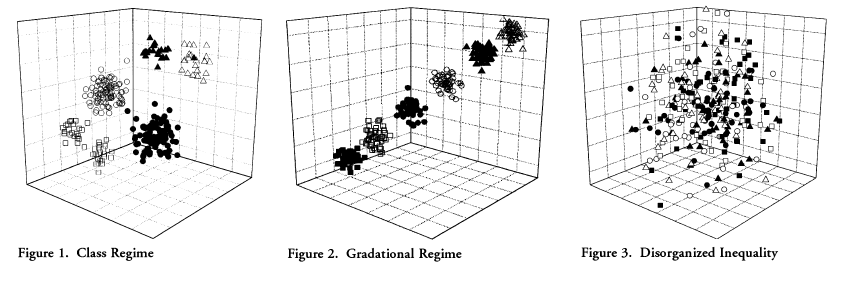
\includegraphics[width=0.8\linewidth]{imagenes/grusky2} 

}

\caption{Tipos de representación de la estructura social (Grusky, 2008): 1) Régimen de clase, 2) Régimen gradacional, 3) Desigualdad desorganizada}\label{fig:xgrusky}
\end{figure}

Mientras que el primero de los gráficos hace referencia a los enfoque clásicos \textbf{relacionales de clase}, en donde las distintas posiciones no pueden representarse en términos de ``más altas'' o ``más bajas'', sino de acuerdo a las múltiples relaciones que se dan entre los grupos, el segundo gráfico hace referencia al enfoque \textbf{estructura funcionalista}, en el que las posiciones son pensadas en términos gradacionales y la distribución respecto a las oportunidades de vida se da en forma ordenada. Finalmente, en el tercer gráfico, se muestra la representación del enfoque que señala el \textbf{debilitamiento de la clase} como factor explicativo de las desigualdades, ante la aparición de múltiples aspectos y factores de mayor relevancia. En este sentido, la desigualdad se torna, en parte, irrepresentable y desorganizada a partir de características de raigambre más individual.

\hypertarget{explorando}{%
\subsection{Explorando los datos por clase social}\label{explorando}}

Al estudiar las desigualdades desde una perspectiva de clases, una primera aproximación al problema puede comenzar explorando el modo en que los distintos indicadores, que consideramos como variables dependientes, se distribuyen entre las distintas posiciones. En este sentido, las medidas de tendencia central, así como las de dispersión, pueden ser buenas herramientas en esta etapa.

Tomando como variable dependiente los ingresos totales individuales (\texttt{P47T}), calcularemos el promedio por clase social. Para ello utilizaremos algunas funciones del paquete \texttt{dplyr} y de \texttt{R\ base} como \texttt{weighted.mean}. Tomaremos como punto de partida, los datos que hemos trabajado en los capítulos anteriores de la \textbf{EPH} del segundo trimestre de 2015.

\begin{Shaded}
\begin{Highlighting}[]
\NormalTok{eph\_ind\_215 }\SpecialCharTok{\%\textgreater{}\%}
    \FunctionTok{filter}\NormalTok{(}\SpecialCharTok{!}\FunctionTok{is.na}\NormalTok{(clase6\_factor)) }\SpecialCharTok{\%\textgreater{}\%}
    \FunctionTok{group\_by}\NormalTok{(clase6\_factor) }\SpecialCharTok{\%\textgreater{}\%}
    \FunctionTok{summarise}\NormalTok{(}\AttributeTok{media =} \FunctionTok{weighted.mean}\NormalTok{(P47T, }\AttributeTok{w =}\NormalTok{ PONDERA))}
\end{Highlighting}
\end{Shaded}

\begin{verbatim}
# A tibble: 6 x 2
  clase6_factor                           media
  <fct>                                   <dbl>
1 Clase alta                             15723.
2 Clase media - autónoma                  8527.
3 Clase media - asalariada                9738.
4 Clase obrera - autónoma                 5509.
5 Clase obrera - asalariada               7151.
6 Clase obrera - trabajadores marginales  3792.
\end{verbatim}

Como puede observarse, las posiciones de clase son explicativas de la desigualdad de ingresos. A mayor posición de clase, mayores ingresos percibidos. A su vez, existen fronteras, en términos de ingresos, entre la clase media y obrera, así como entre los estratos autónomos y asalariados. Sin embargo, la media es una medida que no da una caracterización completa respecto a la distribución de los valores. Para ello comúnmente se utilizan las medidas de posición y de dispersión como forma de conocer cuán homogéneas o heterogéneas son las distribuciones de los datos, en este caso, de los ingresos. El diagramas de caja (o en inglés \emph{boxplot}), nos permite a partir de una salida gráfica, dar cuenta de una serie de estas medidas. Con ayuda del paquete \texttt{ggplot2} y la función \emph{geom\_boxplot} presentamos el siguiente gráfico. Para facilitar la visualización, seleccionamos únicamente los casos con ingresos hasta \texttt{\$40.000}.

\begin{Shaded}
\begin{Highlighting}[]
\NormalTok{eph\_ind\_215 }\SpecialCharTok{\%\textgreater{}\%}
    \FunctionTok{filter}\NormalTok{(}\SpecialCharTok{!}\FunctionTok{is.na}\NormalTok{(clase6\_factor), P47T }\SpecialCharTok{\textless{}=} \DecValTok{40000}\NormalTok{) }\SpecialCharTok{\%\textgreater{}\%}
    \FunctionTok{ggplot}\NormalTok{(}\FunctionTok{aes}\NormalTok{(}\AttributeTok{x =}\NormalTok{ clase6\_factor, }\AttributeTok{y =}\NormalTok{ P47T, }\AttributeTok{fill =}\NormalTok{ clase6\_factor, }\AttributeTok{weight =}\NormalTok{ PONDERA)) }\SpecialCharTok{+}
    \FunctionTok{geom\_boxplot}\NormalTok{(}\AttributeTok{outlier.alpha =} \FloatTok{0.1}\NormalTok{, }\AttributeTok{show.legend =} \ConstantTok{FALSE}\NormalTok{) }\SpecialCharTok{+} \FunctionTok{labs}\NormalTok{(}\AttributeTok{y =} \StringTok{"Ingresos totales individuales"}\NormalTok{,}
    \AttributeTok{caption =} \StringTok{"Elaboración propia en base a EPH{-}INDEC 2015"}\NormalTok{) }\SpecialCharTok{+} \FunctionTok{theme}\NormalTok{(}\AttributeTok{plot.caption =} \FunctionTok{element\_text}\NormalTok{(}\AttributeTok{size =} \DecValTok{9}\NormalTok{),}
    \AttributeTok{axis.title.x =} \FunctionTok{element\_blank}\NormalTok{(), }\AttributeTok{axis.title.y =} \FunctionTok{element\_text}\NormalTok{(}\AttributeTok{size =} \DecValTok{10}\NormalTok{), }\AttributeTok{axis.text.x =} \FunctionTok{element\_text}\NormalTok{(}\AttributeTok{size =} \DecValTok{10}\NormalTok{),}
    \AttributeTok{axis.text.y =} \FunctionTok{element\_text}\NormalTok{(}\AttributeTok{size =} \DecValTok{10}\NormalTok{)) }\SpecialCharTok{+} \FunctionTok{scale\_x\_discrete}\NormalTok{(}\AttributeTok{labels =} \ControlFlowTok{function}\NormalTok{(x) }\FunctionTok{str\_wrap}\NormalTok{(x,}
    \AttributeTok{width =} \DecValTok{20}\NormalTok{)) }\SpecialCharTok{+} \FunctionTok{scale\_y\_continuous}\NormalTok{(}\AttributeTok{breaks =} \FunctionTok{seq}\NormalTok{(}\DecValTok{0}\NormalTok{, }\DecValTok{50000}\NormalTok{, }\DecValTok{5000}\NormalTok{))}
\end{Highlighting}
\end{Shaded}

\begin{figure}

{\centering 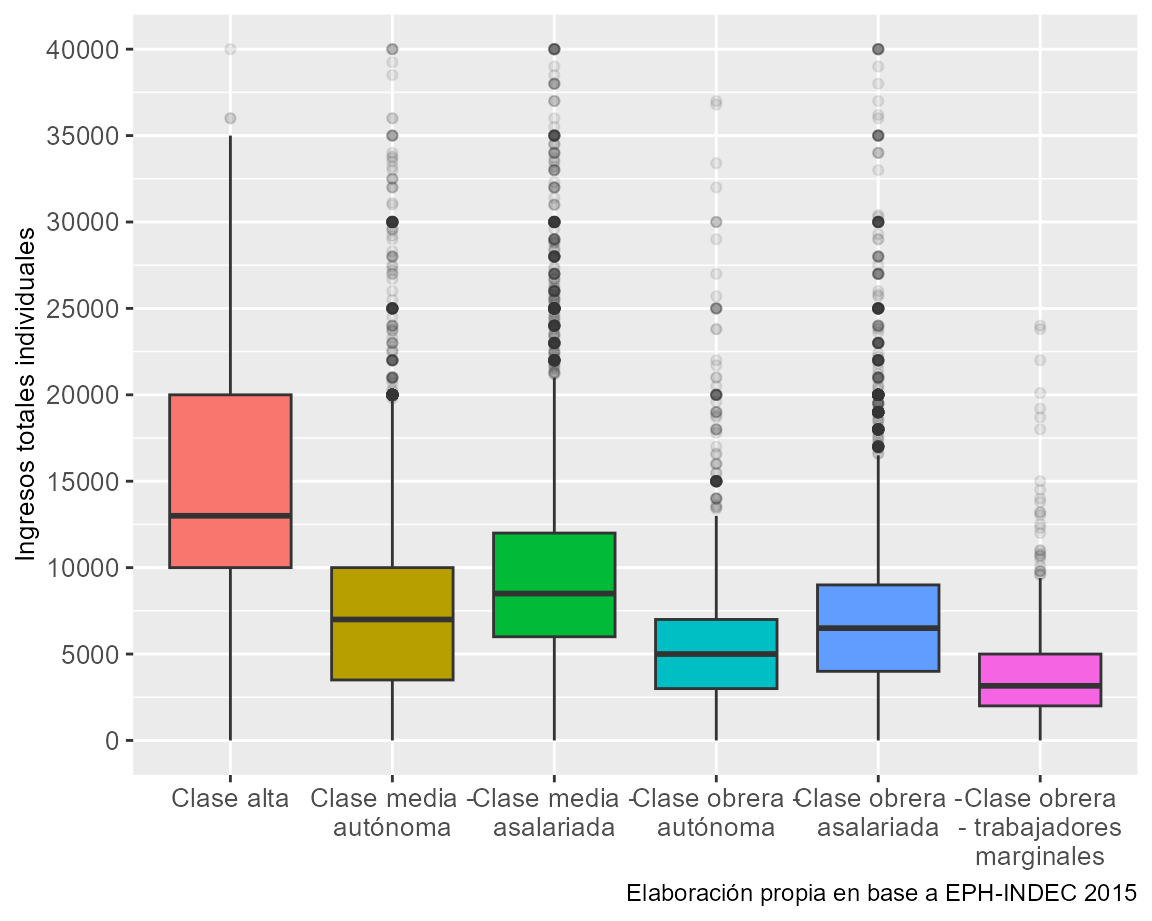
\includegraphics{docs_files/figure-latex/unnamed-chunk-81-1} 

}

\caption{Ingresos totales individuales por clase social}\label{fig:unnamed-chunk-81}
\end{figure}

Varios son los elementos del gráfico que debemos destacar. En primer lugar, las cajas dan cuenta del rango inter-cuartil (1ro y 3ro), mientras que las lineas representan a las medianas de ingresos, es decir, el valor que parte a la distribución por la mitad. De esta forma, los resultados se muestran similares a los arribados en la tabla anterior, aunque las clases medias y la clase alta muestran cierta heterogeneidad en los ingresos percibidos. Finalmente, los límites de las lineas verticales representan los valores máximos y mínimos, mientras que los puntos identifican a los casos atípicos.

\hypertarget{aprox}{%
\subsection{Aproximación al análisis multidimensional}\label{aprox}}

Por último en este capítulo revisaremos un breve ejemplo de análisis multidimensional. Este tipo de abordaje es el más completo para el estudio de las relaciones entre variables, ya que raramente la realidad social puede ser estudiada únicamente a partir de un análisis bivariado. La multicausalidad de los procesos sociales obliga a trabajar con abordajes que permitan captar la mayor cantidad de relaciones, manteniendo siempre la premisa de buscar explicaciones parsimoniosas.

En este sentido, existen distintas técnicas para abordar fenómenos multidimensionales, que dependerán de nuestros objetivos de investigación, tipos de variables, tipos de relaciones, fuente de datos, etc. Podemos nombrar las siguientes: tablas de contingencias múltiples, análisis de la varianza, regresión lineal múltiple, regresión logística, análisis de componentes principales, análisis de correspondencias múltiples, entre otros.

En este caso, retomaremos el ejemplo abordado en el apartado anterior: el vínculo entre la posición de clase y los ingresos. Pero, para completar el análisis, indagaremos también la influencia que tiene el género, la región de residencia y la edad en la captación de ingresos. Como puede verse, el análisis se torna mucho más completo agregando dichas variables.

Debido a que el tipo de variable dependiente con la que contamos (ingresos totales individuales) es cuantitativa, optaremos por emplear un análisis de \emph{regresión lineal múltiple}. No entraremos en detalle sobre lo que implica dicha técnica, pero básicamente nos permitirá:\\
1. estimar la fuerza que cada variable presenta en la relación de dependencia,\\
2. realizar pronósticos sobre cómo se comportan las variables,\\
3. inferenciar al universo de estudio los resultados del modelo aplicado.

Como medida global, podremos obtener un coeficiente de bondad de ajuste que nos guiará sobre cuánto se aleja nuestro modelo respecto a la realidad social relevada por la encuesta.

En primer lugar para plantear un modelo de regresión, debemos configurar aquellas variables que son categóricas para que la función las pueda captar del modo correcto. Básicamente lo que necesitamos es transformar las variables cualitativas a factores. En este caso, solo debemos hacerlo con la variable \emph{REGION} y \emph{CH04} (sexo). Le tendremos que señalar la etiqueta o valor que tomara cada categoría en la nueva variable factor. Asimismo, indicaremos mediante la función \emph{relevel} que para la variable de clase queremos tomar como categoría de referencia a la \emph{Clase obrera - trabajadores marginales}. A continuación explicaremos porque.

\begin{Shaded}
\begin{Highlighting}[]
\NormalTok{eph\_ind\_215}\SpecialCharTok{$}\NormalTok{region\_f }\OtherTok{\textless{}{-}} \FunctionTok{factor}\NormalTok{(eph\_ind\_215}\SpecialCharTok{$}\NormalTok{REGION, }\AttributeTok{labels =} \FunctionTok{c}\NormalTok{(}\StringTok{"GBA"}\NormalTok{, }\StringTok{"NOA"}\NormalTok{, }\StringTok{"NEA"}\NormalTok{,}
    \StringTok{"Cuyo"}\NormalTok{, }\StringTok{"Pampeana"}\NormalTok{, }\StringTok{"Patagónica"}\NormalTok{))}

\NormalTok{eph\_ind\_215}\SpecialCharTok{$}\NormalTok{sexo\_f }\OtherTok{\textless{}{-}} \FunctionTok{factor}\NormalTok{(eph\_ind\_215}\SpecialCharTok{$}\NormalTok{CH04, }\AttributeTok{labels =} \FunctionTok{c}\NormalTok{(}\StringTok{"Varón"}\NormalTok{, }\StringTok{"Mujer"}\NormalTok{))}

\NormalTok{eph\_ind\_215}\SpecialCharTok{$}\NormalTok{clase6\_factor }\OtherTok{\textless{}{-}} \FunctionTok{relevel}\NormalTok{(eph\_ind\_215}\SpecialCharTok{$}\NormalTok{clase6\_factor, }\AttributeTok{ref =} \StringTok{"Clase obrera {-} trabajadores marginales"}\NormalTok{)}
\end{Highlighting}
\end{Shaded}

Realizado estos ajustes, estamos en condiciones de aplicar la regresión lineal múltiple. Antes, guardaremos en un nuevo \texttt{data\ frame} la selección de casos con la que venimos trabajando. La función a utilizar será \emph{lm} (Linear Models), en donde deberemos primero señalar la variable dependiente (P47T) y seguido del símbolo \texttt{\textasciitilde{}} pondremos todas las variables independientes. Al final indicaremos la base sobre la que estamos trabajando. Cada modelo debe ser guardado en un objeto y luego debe ser llamado mediante la función \emph{summary}. Nuestro primer modelo solo medirá la influencia de la clase social sobre los ingresos.

\begin{Shaded}
\begin{Highlighting}[]
\NormalTok{eph\_regresion }\OtherTok{\textless{}{-}}\NormalTok{ eph\_ind\_215 }\SpecialCharTok{\%\textgreater{}\%}
    \FunctionTok{filter}\NormalTok{(CH06 }\SpecialCharTok{\textgreater{}=} \DecValTok{20} \SpecialCharTok{\&}\NormalTok{ ESTADO }\SpecialCharTok{==} \DecValTok{1} \SpecialCharTok{\&} \SpecialCharTok{!}\FunctionTok{is.na}\NormalTok{(clase6\_factor))}

\NormalTok{regresion1 }\OtherTok{\textless{}{-}} \FunctionTok{lm}\NormalTok{(P47T }\SpecialCharTok{\textasciitilde{}}\NormalTok{ clase6\_factor, }\AttributeTok{data =}\NormalTok{ eph\_regresion, }\AttributeTok{weights =}\NormalTok{ PONDERA)}
\FunctionTok{summary}\NormalTok{(regresion1)}
\end{Highlighting}
\end{Shaded}

\begin{verbatim}

Call:
lm(formula = P47T ~ clase6_factor, data = eph_regresion, weights = PONDERA)

Weighted Residuals:
LABEL: MONTO DE INGRESO TOTAL INDIVIDUAL(sumatoria ingresos laborales y no laborales). 
VALUES:
-548054, -58009, -17814, 29883, 3784597

Coefficients:
                                       Estimate Std. Error t value Pr(>|t|)
(Intercept)                                3848        145   26.51   <2e-16
clase6_factorClase alta                   12015        584   20.56   <2e-16
clase6_factorClase media - autónoma        4817        179   26.88   <2e-16
clase6_factorClase media - asalariada      6007        158   38.02   <2e-16
clase6_factorClase obrera - autónoma       1714        192    8.95   <2e-16
clase6_factorClase obrera - asalariada     3480        160   21.80   <2e-16

Residual standard error: 125000 on 23764 degrees of freedom
Multiple R-squared:  0.0921,    Adjusted R-squared:  0.0919 
F-statistic:  482 on 5 and 23764 DF,  p-value: <2e-16
\end{verbatim}

Para simplificar el análisis vamos a prestarle atención a tres cuestiones. En primer lugar, la \textbf{significatividad estadística}, calculada a partir de los valores \textbf{t} y la última columna (estrellas), nos señalan que todas las categorías de la variable clase son significativas. Es decir, que podemos inferir los resultados al total del universo sobre el que se hizo nuestra muestra.

En segundo lugar, tendremos que observar cada uno de los coeficientes \(\beta\) (beta) de la columna \emph{estimate}. Nos señalan en cuánto se incrementan los ingresos respecto a nuestra categoría de referencia. Recordemos que anteriormente configuramos para que nuestra categoría de referencia sea la clase obrera - trabajadores marginales. Esto implica a decir que las personas de clase alta ganan, en promedio estimado, \texttt{\$12.014} más que los trabajadores marginales o \texttt{\$6.007} en el caso de la clase media asalariada.

En tercer lugar, debemos prestar atención a la bondad de ajuste del modelo. Esta se mide a partir del \texttt{R2} (coeficiente de determinación) y lo encontramos en la leyenda inferior de la tabla. Tomando el valor ajustado (\emph{Adjusted R-squared}) y porcentualizándolo, podemos decir que la clase social explica un 9\% de la distribución de los ingresos en la población. El restante 91\% es lo que queda por indagar para saber que otras variables se encargan de explicarlo.

De esta forma, realizamos un segundo modelo (\texttt{regresion2}) en donde incorporamos a los factores edad, región y sexo.

\begin{Shaded}
\begin{Highlighting}[]
\NormalTok{regresion2 }\OtherTok{\textless{}{-}} \FunctionTok{lm}\NormalTok{(P47T }\SpecialCharTok{\textasciitilde{}}\NormalTok{ clase6\_factor }\SpecialCharTok{+}\NormalTok{ CH06 }\SpecialCharTok{+}\NormalTok{ region\_f }\SpecialCharTok{+}\NormalTok{ sexo\_f, }\AttributeTok{data =}\NormalTok{ eph\_regresion,}
    \AttributeTok{weights =}\NormalTok{ PONDERA)}
\FunctionTok{summary}\NormalTok{(regresion2)}
\end{Highlighting}
\end{Shaded}

\begin{verbatim}

Call:
lm(formula = P47T ~ clase6_factor + CH06 + region_f + sexo_f, 
    data = eph_regresion, weights = PONDERA)

Weighted Residuals:
LABEL: MONTO DE INGRESO TOTAL INDIVIDUAL(sumatoria ingresos laborales y no laborales). 
VALUES:
-567092, -51654, -13290, 29441, 3730405

Coefficients:
                                       Estimate Std. Error t value Pr(>|t|)
(Intercept)                             1824.69     202.88    8.99  < 2e-16
clase6_factorClase alta                10933.10     556.07   19.66  < 2e-16
clase6_factorClase media - autónoma     3572.15     174.27   20.50  < 2e-16
clase6_factorClase media - asalariada   5610.99     152.77   36.73  < 2e-16
clase6_factorClase obrera - autónoma     100.75     189.47    0.53    0.595
clase6_factorClase obrera - asalariada  2420.17     160.70   15.06  < 2e-16
CH06                                      95.94       2.92   32.82  < 2e-16
region_fNOA                            -1722.77     128.08  -13.45  < 2e-16
region_fNEA                            -2033.19     179.94  -11.30  < 2e-16
region_fCuyo                            -748.05     148.26   -5.05  4.6e-07
region_fPampeana                        -228.72      90.34   -2.53    0.011
region_fPatagónica                      3862.20     191.59   20.16  < 2e-16
sexo_fMujer                            -2106.44      79.63  -26.45  < 2e-16

Residual standard error: 119000 on 23757 degrees of freedom
Multiple R-squared:  0.181, Adjusted R-squared:  0.181 
F-statistic:  438 on 12 and 23757 DF,  p-value: <2e-16
\end{verbatim}

Todas las categorías resultan significativas, salvo la clase obrera - autónoma. Los coeficientes de la variable clase se mantienen con la misma tendencia (``a mayor clase, mayor ingreso''), aunque sus efectos son un poco menores. La variable CH06 (edad) al ser cuantitativa es de fácil lectura: por cada año adicional de las personas, los ingresos se incrementan en \texttt{\$96}. Respecto a la región, la categoría de referencia es el \texttt{GBA}, ya que no está presente en el cuadro. Todas las regiones deben compararse con esa. De este modo, las personas que viven en \texttt{NOA}, \texttt{NEA}, \texttt{Cuyo} o \texttt{Pampeana}, en promedio ganan menos que los que residen en \texttt{GBA} (ver signo negativo). Los únicos residentes que parecieran tener un ingreso superior que los habitantes del GBA, son los de la región patagónica, con un monto que los supera en \texttt{\$3.862}. El último coeficiente compara los ingresos de las mujeres con los varones, ganando estás últimas, en promedio, \texttt{\$2.106} menos.

Finalmente, la bondad de ajuste mejora considerablemente, al presentarse un \texttt{R2} de \texttt{18,06\%}. Aún queda varianza por ser explicada por otros factores, pero aquellos que hemos incorporado suman significativamente a la explicación de la desigualdad de ingresos.

\hypertarget{dependiente}{%
\section{La clase como variable dependiente}\label{dependiente}}

Este capítulo tiene como propósito presentar una de las posibles aproximaciones al estudio de la estructura de clases en tanto variable dependiente. Dentro de este tipo de abordajes nos preguntamos acerca de aquellos factores que explican, condicionan o intervienen en el proceso de formación y acción de las clases sociales. En este caso nos centraremos en el estudio de la movilidad social, en tanto proceso que permite comprender el modo en que la estructura de clases se configura en el tiempo.

Para ello exploraremos algunas enfoques teóricos que han intentado explicar distintos aspectos de la movilidad social. Posteriormente nos centraremos en el análisis absoluto de la movilidad social a partir de tablas de contingencia y, luego, revisaremos brevemente algunas potencialidades del análisis multivariable del fenómeno. Para ello exploraremos algunas enfoques teóricos que han intentado explicar distintos aspectos de la movilidad social. Posteriormente nos centraremos en el análisis absoluto de la movilidad social a partir de tablas de contingencia y, luego, revisaremos algunas potencialidades del análisis multivariable del fenómeno.

Estas serán algunas de las preguntas que guiarán este capítulo:\\
- ¿Cuáles son las principales perspectivas teóricas que han estudiado el problema de la movilidad social? ¿En qué aspectos se centran para el estudio de la misma?\\
- ¿Qué dimensiones pueden estudiarse para comprender la movilidad social? ¿Qué rol juega la educación en dicho proceso?\\
- ¿Qué tendencias pueden observarse desde una tabla de movilidad social? ¿Que implica la movilidad ascendente, descendente y la reproducción?
- ¿Qué potencialidades ofrece el análisis multivariable de la movilidad social? ¿Qué técnicas pueden utilizarse?

Al completar este capítulo se espera que los lectores puedan:

\begin{enumerate}
\def\labelenumi{\arabic{enumi}.}
\tightlist
\item
  Conocer los principales enfoque teóricos desde donde se ha estudiado la movilidad social (estructural-funcionalismo y enfoque de clases).\\
\item
  Presentar el estudio de la movilidad a través del análisis de tablas de contingencia.\\
\item
  Introducir el enfoque multivariable en el estudio de la movilidad social utilizando como técnica a la regresión logística.
\end{enumerate}

Para una mayor comprensión del capítulo recomendamos la lectura de los siguientes textos:

\begin{itemize}
\item
  Kerbo, H. R. (\protect\hyperlink{ref-Kerbo2003}{2003}). Estratificación social y desigualdad: El conflicto de clases en perspectiva histórica y comparada. Madrid: McGraw-Hill Interamericana de España. \textbf{(Capítulo 6)}
\item
  Dalle, P., Jorrat, J. R., y Riveiro, M. (\protect\hyperlink{ref-Dalle.etal2018}{2018}). Movilidad social intergeneracional. En A. Salvia y J. I. Piovani (Eds.), La Argentina en el siglo XXI. Cómo somos, vivimos y convivimos en una sociedad desigual. Encuesta Nacional sobre la Estructura Social. Buenos Aires: Siglo Veintiuno Editores.
\item
  Solís, P., y Boado, M. (\protect\hyperlink{ref-Solis.Boado2016}{2016}). Y sin embargo se mueve. Estratificación y movilidad intergeneracional de clase en América Latina. México: Centro de Estudios Espinosa Yglesias. \textbf{(Capítulo 1)}
\item
  Pla, J., y Rodríguez de la Fuente, J. J. (\protect\hyperlink{ref-Pla.RodriguezdelaFuente2016}{2016}). Tendencias de movilidad social en la Argentina de las dos últimas décadas: 1995-2010. Papers. Revista de Sociologia, 101(4), 473-502.
\item
  Dalle, P. (\protect\hyperlink{ref-Dalle2016}{2016}). Movilidad social desde las clases populares: Un estudio sociológico en el Área Metropolitana de Buenos Aires 1960-2013. Buenos Aires: IIGG-CLACSO. \textbf{(Capítulo 6 - ejemplo del uso de regresión logística)}
\end{itemize}

\hypertarget{movilidad1}{%
\subsection{El estudio de la movilidad social}\label{movilidad1}}

Como señala Carabaña (\protect\hyperlink{ref-Carabana1997}{1997}) en el estudio de las clases sociales existen dos grandes abordajes posibles: considerar a la clase como una variable independiente o como una variable dependiente. El primero de estos abordajes fue retomado en el \protect\hyperlink{independiente}{Capítulo 7}, denominado por el autor como \emph{análisis de clase}, nos permite comprender cómo los comportamientos sociales pueden ser explicados desde el posicionamiento de clase. Por el contrario, el segundo enfoque, denominado por Carabaña como \emph{teoría de clases}, hace referencia a las explicaciones sobre el surgimiento, la reproducción y la transformación de las clases sociales.

Si bien el mismo no aclara si los estudios de movilidad social se engloban dentro de este segundo abordaje, podemos así considerarlo, ya que nos permite el análisis de las transformaciones y reproducciones dentro del sistema de estratificación. El estudio de la movilidad social nos ayuda a comprender cuánto cambio la estructura de clases respecto a la de generaciones pasadas, así como qué rasgos de la estructura actual se mantienen tal como existían en el pasado.

Vale señalar que el estudio de la clase social como variable dependiente no se acota al análisis de la movilidad social, sino que otros factores pueden ser considerados como explicativos de la misma, tales como la dinámica demográfica, los cambios tecnológicos, las políticas económicas, etc.

\hypertarget{quuxe9-es-la-movilidad-social}{%
\subsubsection{¿Qué es la movilidad social?}\label{quuxe9-es-la-movilidad-social}}

El estudio de la movilidad social adquiere sentido dentro del campo teórico de la estratificación social (\protect\hyperlink{ref-Cortes.Solis2006}{Cortés \& Solís, 2006}), ya que el primer paso es tener noción sobre cómo la sociedad se estructura en grupos o clases. Siguiendo la clásica definición de Lipset y Bendix (\protect\hyperlink{ref-Lipset.Bendix1963}{1963, p. 18}), podemos entender a la movilidad social como el ``proceso por el cual los individuos pasan de una posición a otra en la sociedad''. Al referirnos a \emph{posición}, la literatura admite varias nociones: clases sociales, ocupaciones, niveles de ingresos, niveles de riqueza, niveles de condiciones de vida, niveles educativos, etc. Asimismo, la movilidad puede medirse en términos \textbf{intergeneracionales} (cambios en la posición de los hijos respecto de los padres) o \textbf{intrageneracionales} (cambios en la trayectoria de clase en la vida de la persona). En esta unidad nos centraremos en la \textbf{movilidad intergeneracional de clase}.

En forma simplificada, los estudios clásicos de movilidad social planteaban el abordaje de tres instituciones centrales en la vida de las personas: la familia, la educación y el mercado de trabajo. Esto derivó en lo que se denominó como ``triángulo de la movilidad''.

Generalmente las investigaciones realizadas en este campo han hecho foco en algunas de las relaciones planteadas en dicho triángulo. La mayor parte de los estudios de movilidad se han centrado en la influencia del origen de clase sobre el destino de clase, considerando a la educación con un aspecto a controlar e influyente. Mientras menor sea la influencia del origen de clase sobre el destino y sobre el logro educativo, y mayor el impacto del nivel educativo alcanzado sobre el destino de clase, se estará en mayores condiciones de plantear una situación de \emph{igualdad de oportunidades} para los individuos. Por el contrario, un mayor peso de las condiciones de origen sobre el logro educativo y el destino de clase señala una mayor reproducción en las \emph{desigualdades de condiciones} y una menor igualdad de oportunidades. Mientras que los teóricos estructural funcionalistas hicieron más foco en la primera de estas situaciones, los enfoques críticos desde la teoría de clases hicieron hincapié sobre el segundo aspecto.

Sin embargo los estudios de movilidad social no se han centrado únicamente en el análisis de la influencia del origen social y el logro educativo sobre el destino de clase, sino que también se han incorporado otras dimensiones intervinientes: género, edad, etnia, país de nacimiento, entre otros.

\hypertarget{enfoques-funcionalistas}{%
\subsubsection{Enfoques funcionalistas}\label{enfoques-funcionalistas}}

La sociología de la movilidad social nace al calor del debate sobre la igualdad y en el seno del estructural-funcionalismo. Sus bases conceptuales se sustentan en la concepción liberal del orden social. Acorde con la teoría de la estratificación, la visión liberal-funcionalista comprendía a la sociedad como un campo continuo y homogéneo formado por individuos que desempeñan funciones de más o menos prestigio y remuneración, y que presentan amplias posibilidades de movilidad (\protect\hyperlink{ref-CachonRodriguez1989}{Cachón Rodríguez, 1989}; \protect\hyperlink{ref-Kerbo2003}{Kerbo, 2003}).

Los primeros estudios de movilidad llevados a cabo por encuestas tuvieron lugar en el período de la segunda posguerra y sus preocupaciones giraban en torno a los niveles de movilidad que presentaban los distintos países y sobre la forma que la misma asumía. La \textbf{tabla de movilidad} ---como se ilustra tabla siguiente---, para esta generación, constituye el insumo central para el estudio del fenómeno, conteniendo la misma la información sobre la posición social de las personas a las cuales se encuestó y la posición de su familia (generalmente del padre) cuando éstas tenían alrededor de 15 años (\protect\hyperlink{ref-Breen2004}{Breen, 2004, p. 3}):

\global\setlength{\Oldarrayrulewidth}{\arrayrulewidth}

\global\setlength{\Oldtabcolsep}{\tabcolsep}

\setlength{\tabcolsep}{0pt}

\renewcommand*{\arraystretch}{1.5}



\providecommand{\ascline}[3]{\noalign{\global\arrayrulewidth #1}\arrayrulecolor[HTML]{#2}\cline{#3}}

\begin{longtable}[c]{cccccccc}





\multicolumn{8}{>{}l}{\textcolor[HTML]{000000}{\fontsize{10}{10}\selectfont{Fuente:\ Dalle\ (2016),\ en\ base\ a\ Encuestas\ del\ CEDEP-UBA}}} \\

\endfoot

\ascline{1pt}{000000}{1-8}

\multicolumn{1}{!{\color[HTML]{000000}\vrule width 1pt}>{}l}{} & \multicolumn{7}{!{\color[HTML]{000000}\vrule width 1pt}>{}l!{\color[HTML]{000000}\vrule width 1pt}}{\textcolor[HTML]{000000}{\fontsize{10}{10}\selectfont{Posición\ de\ clase\ del\ encuestado}}} \\

\ascline{1pt}{000000}{2-8}



\multicolumn{1}{!{\color[HTML]{000000}\vrule width 1pt}>{}l}{\multirow[c]{-2}{*}{\parbox{0.75in}{\raggedright \textcolor[HTML]{000000}{\fontsize{10}{10}\selectfont{Posición\ de\ clase\ del\ padre}}}}} & \multicolumn{1}{!{\color[HTML]{000000}\vrule width 1pt}>{}l}{\textcolor[HTML]{000000}{\fontsize{10}{10}\selectfont{Clase\ media\ prof.\ y\ gerencial}}} & \multicolumn{1}{!{\color[HTML]{000000}\vrule width 1pt}>{}l}{\textcolor[HTML]{000000}{\fontsize{10}{10}\selectfont{Pequeños\ prop.\ de\ capital}}} & \multicolumn{1}{!{\color[HTML]{000000}\vrule width 1pt}>{}l}{\textcolor[HTML]{000000}{\fontsize{10}{10}\selectfont{Clase\ intermedia\ técnica\ adm.}}} & \multicolumn{1}{!{\color[HTML]{000000}\vrule width 1pt}>{}l}{\textcolor[HTML]{000000}{\fontsize{10}{10}\selectfont{Clase\ popular\ calificada}}} & \multicolumn{1}{!{\color[HTML]{000000}\vrule width 1pt}>{}l}{\textcolor[HTML]{000000}{\fontsize{10}{10}\selectfont{Clase\ popular\ no\ calificada}}} & \multicolumn{1}{!{\color[HTML]{000000}\vrule width 1pt}>{}l}{\textcolor[HTML]{000000}{\fontsize{10}{10}\selectfont{Total}}} & \multicolumn{1}{!{\color[HTML]{000000}\vrule width 1pt}>{}l!{\color[HTML]{000000}\vrule width 1pt}}{\textcolor[HTML]{000000}{\fontsize{10}{10}\selectfont{n}}} \\

\ascline{1pt}{000000}{1-8}



\multicolumn{1}{!{\color[HTML]{000000}\vrule width 1pt}>{}l}{\textcolor[HTML]{000000}{\fontsize{10}{10}\selectfont{Clase\ media\ profesional\ y\ gerencial}}} & \multicolumn{1}{!{\color[HTML]{000000}\vrule width 1pt}>{}l}{\textcolor[HTML]{000000}{\fontsize{10}{10}\selectfont{34,6}}} & \multicolumn{1}{!{\color[HTML]{000000}\vrule width 1pt}>{}l}{\textcolor[HTML]{000000}{\fontsize{10}{10}\selectfont{6,4}}} & \multicolumn{1}{!{\color[HTML]{000000}\vrule width 1pt}>{}l}{\textcolor[HTML]{000000}{\fontsize{10}{10}\selectfont{44,9}}} & \multicolumn{1}{!{\color[HTML]{000000}\vrule width 1pt}>{}l}{\textcolor[HTML]{000000}{\fontsize{10}{10}\selectfont{11,5}}} & \multicolumn{1}{!{\color[HTML]{000000}\vrule width 1pt}>{}l}{\textcolor[HTML]{000000}{\fontsize{10}{10}\selectfont{2,6}}} & \multicolumn{1}{!{\color[HTML]{000000}\vrule width 1pt}>{}l}{\textcolor[HTML]{000000}{\fontsize{10}{10}\selectfont{100,0}}} & \multicolumn{1}{!{\color[HTML]{000000}\vrule width 1pt}>{}l!{\color[HTML]{000000}\vrule width 1pt}}{\textcolor[HTML]{000000}{\fontsize{10}{10}\selectfont{78}}} \\

\ascline{1pt}{000000}{1-8}



\multicolumn{1}{!{\color[HTML]{000000}\vrule width 1pt}>{}l}{\textcolor[HTML]{000000}{\fontsize{10}{10}\selectfont{Pequeños\ propietarios\ de\ capital}}} & \multicolumn{1}{!{\color[HTML]{000000}\vrule width 1pt}>{}l}{\textcolor[HTML]{000000}{\fontsize{10}{10}\selectfont{26,3}}} & \multicolumn{1}{!{\color[HTML]{000000}\vrule width 1pt}>{}l}{\textcolor[HTML]{000000}{\fontsize{10}{10}\selectfont{16,2}}} & \multicolumn{1}{!{\color[HTML]{000000}\vrule width 1pt}>{}l}{\textcolor[HTML]{000000}{\fontsize{10}{10}\selectfont{36,4}}} & \multicolumn{1}{!{\color[HTML]{000000}\vrule width 1pt}>{}l}{\textcolor[HTML]{000000}{\fontsize{10}{10}\selectfont{12,1}}} & \multicolumn{1}{!{\color[HTML]{000000}\vrule width 1pt}>{}l}{\textcolor[HTML]{000000}{\fontsize{10}{10}\selectfont{9,1}}} & \multicolumn{1}{!{\color[HTML]{000000}\vrule width 1pt}>{}l}{\textcolor[HTML]{000000}{\fontsize{10}{10}\selectfont{100,0}}} & \multicolumn{1}{!{\color[HTML]{000000}\vrule width 1pt}>{}l!{\color[HTML]{000000}\vrule width 1pt}}{\textcolor[HTML]{000000}{\fontsize{10}{10}\selectfont{99}}} \\

\ascline{1pt}{000000}{1-8}



\multicolumn{1}{!{\color[HTML]{000000}\vrule width 1pt}>{}l}{\textcolor[HTML]{000000}{\fontsize{10}{10}\selectfont{Clase\ intermedia\ técnica-administrativa}}} & \multicolumn{1}{!{\color[HTML]{000000}\vrule width 1pt}>{}l}{\textcolor[HTML]{000000}{\fontsize{10}{10}\selectfont{25,9}}} & \multicolumn{1}{!{\color[HTML]{000000}\vrule width 1pt}>{}l}{\textcolor[HTML]{000000}{\fontsize{10}{10}\selectfont{9,4}}} & \multicolumn{1}{!{\color[HTML]{000000}\vrule width 1pt}>{}l}{\textcolor[HTML]{000000}{\fontsize{10}{10}\selectfont{44,7}}} & \multicolumn{1}{!{\color[HTML]{000000}\vrule width 1pt}>{}l}{\textcolor[HTML]{000000}{\fontsize{10}{10}\selectfont{11,8}}} & \multicolumn{1}{!{\color[HTML]{000000}\vrule width 1pt}>{}l}{\textcolor[HTML]{000000}{\fontsize{10}{10}\selectfont{8,2}}} & \multicolumn{1}{!{\color[HTML]{000000}\vrule width 1pt}>{}l}{\textcolor[HTML]{000000}{\fontsize{10}{10}\selectfont{100,0}}} & \multicolumn{1}{!{\color[HTML]{000000}\vrule width 1pt}>{}l!{\color[HTML]{000000}\vrule width 1pt}}{\textcolor[HTML]{000000}{\fontsize{10}{10}\selectfont{85}}} \\

\ascline{1pt}{000000}{1-8}



\multicolumn{1}{!{\color[HTML]{000000}\vrule width 1pt}>{}l}{\textcolor[HTML]{000000}{\fontsize{10}{10}\selectfont{Clase\ popular\ calificada}}} & \multicolumn{1}{!{\color[HTML]{000000}\vrule width 1pt}>{}l}{\textcolor[HTML]{000000}{\fontsize{10}{10}\selectfont{10,0}}} & \multicolumn{1}{!{\color[HTML]{000000}\vrule width 1pt}>{}l}{\textcolor[HTML]{000000}{\fontsize{10}{10}\selectfont{3,8}}} & \multicolumn{1}{!{\color[HTML]{000000}\vrule width 1pt}>{}l}{\textcolor[HTML]{000000}{\fontsize{10}{10}\selectfont{32,6}}} & \multicolumn{1}{!{\color[HTML]{000000}\vrule width 1pt}>{}l}{\textcolor[HTML]{000000}{\fontsize{10}{10}\selectfont{29,6}}} & \multicolumn{1}{!{\color[HTML]{000000}\vrule width 1pt}>{}l}{\textcolor[HTML]{000000}{\fontsize{10}{10}\selectfont{24,1}}} & \multicolumn{1}{!{\color[HTML]{000000}\vrule width 1pt}>{}l}{\textcolor[HTML]{000000}{\fontsize{10}{10}\selectfont{100,0}}} & \multicolumn{1}{!{\color[HTML]{000000}\vrule width 1pt}>{}l!{\color[HTML]{000000}\vrule width 1pt}}{\textcolor[HTML]{000000}{\fontsize{10}{10}\selectfont{291}}} \\

\ascline{1pt}{000000}{1-8}



\multicolumn{1}{!{\color[HTML]{000000}\vrule width 1pt}>{}l}{\textcolor[HTML]{000000}{\fontsize{10}{10}\selectfont{Clase\ popular\ no\ calificada}}} & \multicolumn{1}{!{\color[HTML]{000000}\vrule width 1pt}>{}l}{\textcolor[HTML]{000000}{\fontsize{10}{10}\selectfont{2,7}}} & \multicolumn{1}{!{\color[HTML]{000000}\vrule width 1pt}>{}l}{\textcolor[HTML]{000000}{\fontsize{10}{10}\selectfont{8,0}}} & \multicolumn{1}{!{\color[HTML]{000000}\vrule width 1pt}>{}l}{\textcolor[HTML]{000000}{\fontsize{10}{10}\selectfont{20,0}}} & \multicolumn{1}{!{\color[HTML]{000000}\vrule width 1pt}>{}l}{\textcolor[HTML]{000000}{\fontsize{10}{10}\selectfont{30,7}}} & \multicolumn{1}{!{\color[HTML]{000000}\vrule width 1pt}>{}l}{\textcolor[HTML]{000000}{\fontsize{10}{10}\selectfont{38,7}}} & \multicolumn{1}{!{\color[HTML]{000000}\vrule width 1pt}>{}l}{\textcolor[HTML]{000000}{\fontsize{10}{10}\selectfont{100,0}}} & \multicolumn{1}{!{\color[HTML]{000000}\vrule width 1pt}>{}l!{\color[HTML]{000000}\vrule width 1pt}}{\textcolor[HTML]{000000}{\fontsize{10}{10}\selectfont{150}}} \\

\ascline{1pt}{000000}{1-8}



\multicolumn{1}{!{\color[HTML]{000000}\vrule width 1pt}>{}l}{\textcolor[HTML]{000000}{\fontsize{10}{10}\selectfont{Total}}} & \multicolumn{1}{!{\color[HTML]{000000}\vrule width 1pt}>{}l}{\textcolor[HTML]{000000}{\fontsize{10}{10}\selectfont{15,4}}} & \multicolumn{1}{!{\color[HTML]{000000}\vrule width 1pt}>{}l}{\textcolor[HTML]{000000}{\fontsize{10}{10}\selectfont{7,4}}} & \multicolumn{1}{!{\color[HTML]{000000}\vrule width 1pt}>{}l}{\textcolor[HTML]{000000}{\fontsize{10}{10}\selectfont{33,3}}} & \multicolumn{1}{!{\color[HTML]{000000}\vrule width 1pt}>{}l}{\textcolor[HTML]{000000}{\fontsize{10}{10}\selectfont{23,2}}} & \multicolumn{1}{!{\color[HTML]{000000}\vrule width 1pt}>{}l}{\textcolor[HTML]{000000}{\fontsize{10}{10}\selectfont{20,8}}} & \multicolumn{1}{!{\color[HTML]{000000}\vrule width 1pt}>{}l}{\textcolor[HTML]{000000}{\fontsize{10}{10}\selectfont{100,0}}} & \multicolumn{1}{!{\color[HTML]{000000}\vrule width 1pt}>{}l!{\color[HTML]{000000}\vrule width 1pt}}{\textcolor[HTML]{000000}{\fontsize{10}{10}\selectfont{703}}} \\

\ascline{1pt}{000000}{1-8}



\end{longtable}



\arrayrulecolor[HTML]{000000}

\global\setlength{\arrayrulewidth}{\Oldarrayrulewidth}

\global\setlength{\tabcolsep}{\Oldtabcolsep}

\renewcommand*{\arraystretch}{1}

Posteriormente, una segunda oleada de estudios de movilidad social, iniciada con la obra \emph{The American Occupational Structure} (\protect\hyperlink{ref-Blau.Duncan1967}{Blau \& Duncan, 1967}), marcaron un nuevo rumbo teórico y metodológico en el campo. En primer lugar, Blau y Duncan plantearon un abordaje del fenómeno de la movilidad social considerándolo como parte del ``proceso de estratificación''. De este modo descompusieron el concepto en sus elementos constituyentes, es decir, en la posición de origen y de destino. Ya no enfocaron el problema desde el estudio de los patrones de movilidad, sino a partir de los efectos que las características adscriptivas presentaban sobre el logro ocupacional. En términos operativos, la preocupación rondaba en torno a cómo diversos factores intervinientes (principalmente, la educación) y las contingencias de la carrera ocupacional podían modificar la influencia de los orígenes sociales sobre los logros ocupacionales de los sujetos.

El trabajo de Blau y Duncan resaltaba tres aspectos:

\begin{enumerate}
\def\labelenumi{\arabic{enumi}.}
\item
  La utilización como criterio clasificatorio de un índice socio-económico (SEI)\footnote{ver \protect\hyperlink{propuestas-gradacionales}{Capítulo 6}}. Esta elección tenía dos fundamentos. En primer lugar, los autores asumían que la estructura ocupacional se configuraba de una manera más o menos continua, más que en clases discretas y separadas. En segundo lugar, el carácter gradacional era apropiado para la aplicación de determinadas técnicas estadísticas (correlaciones y regresiones) que el modelo analítico requería.
\item
  La utilización de la técnica del \emph{path analysis} (variante de la regresión lineal múltiple) para conocer los efectos directos e indirectos que ejercen cada una de las variables.
\item
  Las conclusiones sobre la preminencia de los procesos de movilidad social en la sociedad estadounidense. \emph{The American Occupational Structure} sentó una serie de conclusiones que demostraban que Estados Unidos era un país en el que el mérito era el principal motor de ascenso social. El nivel educativo de los encuestados era considerado como la principal variable explicativa, por sobre las características de origen (\protect\hyperlink{ref-Blau.Duncan1967}{Blau \& Duncan, 1967, pp. 155, 169--170}).
\end{enumerate}

\hypertarget{enfoques-de-clase}{%
\subsubsection{Enfoques de clase}\label{enfoques-de-clase}}

A partir de los años '70, con el rompimiento del consenso ortodoxo estructural funcionalista, se abre una puerta al pluralismo sociológico en el campo de la movilidad social, a partir de la convivencia de diversas escuelas y tradiciones. Estos enfoques hicieron mayor énfasis en las desigualdades de origen y en la comprensión del fenómeno de la movilidad como un aspecto del proceso de formación y acción de las clases. Desde esta perspectiva general, las chances de movilidad social estarían fuertemente determinadas por las condiciones de origen (\protect\hyperlink{ref-Kerbo2003}{Kerbo, 2003, p. 156}). Asimismo, muchos autores además de situar este abordaje en continuidad con la tradición weberiana, acuerdan que también en los escritos de Marx podría encontrarse cierta preocupación por el fenómeno de la estructura de la movilidad y las desigualdades de origen (\protect\hyperlink{ref-Kerbo2003}{Kerbo, 2003, p. 155}).

La mirada de John Goldthorpe fue una de las más relevantes dentro de este enfoque. Para este autor, la movilidad social es un fenómeno que ocurre en la estructura de clases, es decir, dentro de las relaciones laborales, y no en un continuo de prestigio, estatus o recursos socioeconómicos. Desde el campo técnico también se avanzó a pasos agigantados, al comenzarse a utilizar los \emph{modelos loglineales}. Esta técnica permitió el tratamiento estadístico para evaluar la asociación entre los orígenes y los destinos, a partir de variables discretas, es decir, habilitando la posibilidad de utilizar clasificaciones basadas en esquemas de clases sociales. Este tipo de análisis habilitaba el abordaje multidimensional, acercándose de este modo a las características que proponía el \textbf{path analysis}, incorporándose al análisis las variables de educación, cohorte, género y/o país.

Uno de los grandes aportes a los que Goldthorpe y su equipo arribó, a través del Proyecto \emph{Comparative Study of Social Mobility in Industrial Nations} (CASMIN) que recopiló una serie de encuestas sobre movilidad social de los países con mayores niveles de industrialización de Europa (sumando a Japón y Estados Unidos) de alrededor de la década del '70, fue que la condición de clase de origen, a diferencia de lo postulado en los abordajes funcionalistas, aún continúa teniendo efectos sobre el destino de las personas, y que esto debe ser explicado a partir de las ventajas y desventajas que se asocian a cada posición de clase (\protect\hyperlink{ref-Erikson.Goldthorpe2002}{Erikson \& Goldthorpe, 2002}).

\hypertarget{enes}{%
\subsection{El uso de la base ENES-PISAC}\label{enes}}

Librerías que utilizaremos en esta sección:

\begin{Shaded}
\begin{Highlighting}[]
\FunctionTok{library}\NormalTok{(haven)}
\FunctionTok{library}\NormalTok{(tidyverse, }\AttributeTok{warn.conflicts =} \ConstantTok{FALSE}\NormalTok{)}
\end{Highlighting}
\end{Shaded}

Como hemos señalado en el \protect\hyperlink{otras}{Capítulo 2}, una de las bases de datos públicas y nacionales para el estudio de la movilidad social es la \emph{Encuesta Nacional sobre la Estructura Social} (\textbf{ENES}) desarrollada por el \textbf{Programa de Investigación sobre la Sociedad Argentina Contemporánea}(PISAC). La misma puede ser descargada, junto a los manuales de códigos, siguiendo este \href{https://www.argentina.gob.ar/ciencia/pisac/bases-de-datos}{link}.

Descargaremos las bases de individuos y hogares en formato SPSS.

\hypertarget{algunas-consideraciones-de-la-enes}{%
\subsubsection{Algunas consideraciones de la ENES}\label{algunas-consideraciones-de-la-enes}}

Antes de comenzar a trabajar con la ENES, señalaremos una serie de cuestiones previas a tener en consideración:

\begin{enumerate}
\def\labelenumi{\arabic{enumi}.}
\item
  La encuesta cuenta con información socio-ocupacional para todos los miembros de 10 años y más. A su vez, para el análisis de la movilidad social intergeneracional, cuenta con información sociolaboral sobre el/la Principal Sostén del Hogar (PSH) cuando el/la PSH y/o cónyuge del hogar entrevistado tenían 15 años de edad. En otras palabras, podemos observar los patrones de movilidad tanto del/la PSH y cónyuge del hogar.
\item
  La encuesta ya provee a los usuarios esquemas de clase social construidos (CSO de Torrado y EGP), en formato desagregado, tanto para los miembros del hogar mayores de 10 años ocupados y desocupados, como para el PSH de origen.
\item
  Al igual que con la \textbf{EPH}, necesitaremos pegar la información de la base de hogar en la base de individuos, ya que los datos de movilidad social se encuentra en la primera base.
\end{enumerate}

\hypertarget{abriendo-y-pegando-la-base-enes}{%
\subsubsection{Abriendo y pegando la base ENES}\label{abriendo-y-pegando-la-base-enes}}

Para abrir los archivos \textbf{\texttt{.sav}} nuevamente deberemos llamar al paquete \texttt{haven} que hemos instalado en el \protect\hyperlink{eph2}{Capítulo 3} y utilizaremos la función \emph{read\_sav}.

\begin{Shaded}
\begin{Highlighting}[]
\NormalTok{enes\_ind }\OtherTok{\textless{}{-}} \FunctionTok{read\_sav}\NormalTok{(}\StringTok{"bases/ENES\_Personas\_version\_final.sav"}\NormalTok{)}
\NormalTok{enes\_hog }\OtherTok{\textless{}{-}} \FunctionTok{read\_sav}\NormalTok{(}\StringTok{"bases/ENES\_Hogares\_version\_final.sav"}\NormalTok{)}
\end{Highlighting}
\end{Shaded}

Obtenidos ambos \texttt{datasets} ahora vamos a pegar la base de hogares a la de individuos, utilizando como variables identificadoras a \texttt{nocues} (Código Identificador de Vivienda) y \texttt{nhog} (Código Identificador del Hogar).

\begin{Shaded}
\begin{Highlighting}[]
\NormalTok{enes }\OtherTok{\textless{}{-}}\NormalTok{ enes\_ind }\SpecialCharTok{\%\textgreater{}\%}
    \FunctionTok{left\_join}\NormalTok{(enes\_hog, }\AttributeTok{by =} \FunctionTok{c}\NormalTok{(}\StringTok{"nocues"}\NormalTok{, }\StringTok{"nhog"}\NormalTok{)) }\SpecialCharTok{\%\textgreater{}\%}
    \FunctionTok{select}\NormalTok{(}\SpecialCharTok{!}\NormalTok{(}\FunctionTok{ends\_with}\NormalTok{(}\StringTok{".y"}\NormalTok{)))  }\CommentTok{\#elimina una de las variables que tienen en común las bases y que se duplican.}
\end{Highlighting}
\end{Shaded}

\hypertarget{recodificaciuxf3n-de-variables-y-filtros}{%
\subsubsection{Recodificación de variables y filtros}\label{recodificaciuxf3n-de-variables-y-filtros}}

Para el análisis de la movilidad social que realizaremos en las dos secciones posteriores necesitaremos recodificar una serie de variables para su correcto tratamiento. Empecemos por la principal, la clase social del/la encuestado/o. En este caso nos basaremos en el esquema EGP, que se encuentra codificado en la variable \texttt{egp11} ---Tabla \ref{tab:egpmov}---. Al tenerlo en su versión desagregada de 11 clases, necesitaremos reagruparlo de tal forma que queden 5 clases. A continuación mostramos nuestra propuesta de agrupación y las líneas de comando necesarias para hacerlo:

\global\setlength{\Oldarrayrulewidth}{\arrayrulewidth}

\global\setlength{\Oldtabcolsep}{\tabcolsep}

\setlength{\tabcolsep}{0pt}

\renewcommand*{\arraystretch}{1.5}



\providecommand{\ascline}[3]{\noalign{\global\arrayrulewidth #1}\arrayrulecolor[HTML]{#2}\cline{#3}}

\begin{longtable}[c]{ccc}

\caption{Esquema\ EGP\ recodificado}\label{tab:egpmov}\\



\multicolumn{3}{>{}l}{\textcolor[HTML]{000000}{\fontsize{10}{10}\selectfont{Fuente:\ elaboración\ propia\ en\ base\ Erikson\ y\ Goldthorpe\ (1992)}}} \\

\endfoot

\ascline{1pt}{000000}{1-3}

\multicolumn{1}{!{\color[HTML]{000000}\vrule width 1pt}>{}l}{\textcolor[HTML]{000000}{\fontsize{10}{10}\selectfont{Código}}} & \multicolumn{1}{!{\color[HTML]{000000}\vrule width 1pt}>{}l}{\textcolor[HTML]{000000}{\fontsize{10}{10}\selectfont{Esquema\ 11\ clases}}} & \multicolumn{1}{!{\color[HTML]{000000}\vrule width 1pt}>{}l!{\color[HTML]{000000}\vrule width 1pt}}{\textcolor[HTML]{000000}{\fontsize{10}{10}\selectfont{Esquema\ 5\ clases}}} \\

\ascline{1pt}{000000}{1-3}



\multicolumn{1}{!{\color[HTML]{000000}\vrule width 1pt}>{}l}{\textcolor[HTML]{000000}{\fontsize{10}{10}\selectfont{1}}} & \multicolumn{1}{!{\color[HTML]{000000}\vrule width 1pt}>{}l}{\textcolor[HTML]{000000}{\fontsize{10}{10}\selectfont{I.\ Clase\ de\ servicios,\ alta}}} & \multicolumn{1}{!{\color[HTML]{000000}\vrule width 1pt}>{}l!{\color[HTML]{000000}\vrule width 1pt}}{} \\

\ascline{1pt}{000000}{1-2}



\multicolumn{1}{!{\color[HTML]{000000}\vrule width 1pt}>{}l}{\textcolor[HTML]{000000}{\fontsize{10}{10}\selectfont{2}}} & \multicolumn{1}{!{\color[HTML]{000000}\vrule width 1pt}>{}l}{\textcolor[HTML]{000000}{\fontsize{10}{10}\selectfont{II.\ Clase\ de\ servicios,\ baja}}} & \multicolumn{1}{!{\color[HTML]{000000}\vrule width 1pt}>{}l!{\color[HTML]{000000}\vrule width 1pt}}{\multirow[c]{-2}{*}{\parbox{0.75in}{\raggedright \textcolor[HTML]{000000}{\fontsize{10}{10}\selectfont{Clase\ de\ servicios}}}}} \\

\ascline{1pt}{000000}{1-3}



\multicolumn{1}{!{\color[HTML]{000000}\vrule width 1pt}>{}l}{\textcolor[HTML]{000000}{\fontsize{10}{10}\selectfont{3}}} & \multicolumn{1}{!{\color[HTML]{000000}\vrule width 1pt}>{}l}{\textcolor[HTML]{000000}{\fontsize{10}{10}\selectfont{IIIa.\ Trabajadores\ no\ manuales\ de\ rutina,\ alta}}} & \multicolumn{1}{!{\color[HTML]{000000}\vrule width 1pt}>{}l!{\color[HTML]{000000}\vrule width 1pt}}{} \\

\ascline{1pt}{000000}{1-2}



\multicolumn{1}{!{\color[HTML]{000000}\vrule width 1pt}>{}l}{\textcolor[HTML]{000000}{\fontsize{10}{10}\selectfont{4}}} & \multicolumn{1}{!{\color[HTML]{000000}\vrule width 1pt}>{}l}{\textcolor[HTML]{000000}{\fontsize{10}{10}\selectfont{IIIb.\ Trabajadores\ no\ manuales\ de\ servicios\ y\ comercio,\ baja}}} & \multicolumn{1}{!{\color[HTML]{000000}\vrule width 1pt}>{}l!{\color[HTML]{000000}\vrule width 1pt}}{\multirow[c]{-2}{*}{\parbox{0.75in}{\raggedright \textcolor[HTML]{000000}{\fontsize{10}{10}\selectfont{Trabajadores\ rutinarios}}}}} \\

\ascline{1pt}{000000}{1-3}



\multicolumn{1}{!{\color[HTML]{000000}\vrule width 1pt}>{}l}{\textcolor[HTML]{000000}{\fontsize{10}{10}\selectfont{5}}} & \multicolumn{1}{!{\color[HTML]{000000}\vrule width 1pt}>{}l}{\textcolor[HTML]{000000}{\fontsize{10}{10}\selectfont{IVa.\ Autónomos\ con\ empleados}}} & \multicolumn{1}{!{\color[HTML]{000000}\vrule width 1pt}>{}l!{\color[HTML]{000000}\vrule width 1pt}}{} \\

\ascline{1pt}{000000}{1-2}



\multicolumn{1}{!{\color[HTML]{000000}\vrule width 1pt}>{}l}{\textcolor[HTML]{000000}{\fontsize{10}{10}\selectfont{6}}} & \multicolumn{1}{!{\color[HTML]{000000}\vrule width 1pt}>{}l}{\textcolor[HTML]{000000}{\fontsize{10}{10}\selectfont{IVb.\ Autónomos\ sin\ empleados}}} & \multicolumn{1}{!{\color[HTML]{000000}\vrule width 1pt}>{}l!{\color[HTML]{000000}\vrule width 1pt}}{\multirow[c]{-2}{*}{\parbox{0.75in}{\raggedright \textcolor[HTML]{000000}{\fontsize{10}{10}\selectfont{Pequeña\ Burguesía}}}}} \\

\ascline{1pt}{000000}{1-3}



\multicolumn{1}{!{\color[HTML]{000000}\vrule width 1pt}>{}l}{\textcolor[HTML]{000000}{\fontsize{10}{10}\selectfont{7}}} & \multicolumn{1}{!{\color[HTML]{000000}\vrule width 1pt}>{}l}{\textcolor[HTML]{000000}{\fontsize{10}{10}\selectfont{V.\ Supervisores\ de\ trabajadores\ manuales}}} & \multicolumn{1}{!{\color[HTML]{000000}\vrule width 1pt}>{}l!{\color[HTML]{000000}\vrule width 1pt}}{} \\

\ascline{1pt}{000000}{1-2}



\multicolumn{1}{!{\color[HTML]{000000}\vrule width 1pt}>{}l}{\textcolor[HTML]{000000}{\fontsize{10}{10}\selectfont{8}}} & \multicolumn{1}{!{\color[HTML]{000000}\vrule width 1pt}>{}l}{\textcolor[HTML]{000000}{\fontsize{10}{10}\selectfont{VI.\ Trabajadores\ manuales\ calificados}}} & \multicolumn{1}{!{\color[HTML]{000000}\vrule width 1pt}>{}l!{\color[HTML]{000000}\vrule width 1pt}}{\multirow[c]{-2}{*}{\parbox{0.75in}{\raggedright \textcolor[HTML]{000000}{\fontsize{10}{10}\selectfont{Clase\ trabajadora\ calificada}}}}} \\

\ascline{1pt}{000000}{1-3}



\multicolumn{1}{!{\color[HTML]{000000}\vrule width 1pt}>{}l}{\textcolor[HTML]{000000}{\fontsize{10}{10}\selectfont{9}}} & \multicolumn{1}{!{\color[HTML]{000000}\vrule width 1pt}>{}l}{\textcolor[HTML]{000000}{\fontsize{10}{10}\selectfont{VIIa.\ Trabajadores\ manuales\ no\ calificados}}} & \multicolumn{1}{!{\color[HTML]{000000}\vrule width 1pt}>{}l!{\color[HTML]{000000}\vrule width 1pt}}{} \\

\ascline{1pt}{000000}{1-2}



\multicolumn{1}{!{\color[HTML]{000000}\vrule width 1pt}>{}l}{\textcolor[HTML]{000000}{\fontsize{10}{10}\selectfont{10}}} & \multicolumn{1}{!{\color[HTML]{000000}\vrule width 1pt}>{}l}{\textcolor[HTML]{000000}{\fontsize{10}{10}\selectfont{VIIb.\ Trabajadores\ agropecuarios}}} & \multicolumn{1}{!{\color[HTML]{000000}\vrule width 1pt}>{}l!{\color[HTML]{000000}\vrule width 1pt}}{\multirow[c]{-2}{*}{\parbox{0.75in}{\raggedright \textcolor[HTML]{000000}{\fontsize{10}{10}\selectfont{Clase\ trabajadora\ no\ calificada}}}}} \\

\ascline{1pt}{000000}{1-3}



\multicolumn{1}{!{\color[HTML]{000000}\vrule width 1pt}>{}l}{\textcolor[HTML]{000000}{\fontsize{10}{10}\selectfont{11}}} & \multicolumn{1}{!{\color[HTML]{000000}\vrule width 1pt}>{}l}{\textcolor[HTML]{000000}{\fontsize{10}{10}\selectfont{IVc.\ Autónomos\ agropecuarios}}} & \multicolumn{1}{!{\color[HTML]{000000}\vrule width 1pt}>{}l!{\color[HTML]{000000}\vrule width 1pt}}{\textcolor[HTML]{000000}{\fontsize{10}{10}\selectfont{Pequeña\ Burguesía}}} \\

\ascline{1pt}{000000}{1-3}



\end{longtable}



\arrayrulecolor[HTML]{000000}

\global\setlength{\arrayrulewidth}{\Oldarrayrulewidth}

\global\setlength{\tabcolsep}{\Oldtabcolsep}

\renewcommand*{\arraystretch}{1}

\begin{Shaded}
\begin{Highlighting}[]
\NormalTok{enes }\OtherTok{\textless{}{-}}\NormalTok{ enes }\SpecialCharTok{\%\textgreater{}\%}
    \FunctionTok{mutate}\NormalTok{(}\AttributeTok{egp5 =}\NormalTok{ car}\SpecialCharTok{::}\FunctionTok{recode}\NormalTok{(egp11, }\StringTok{"1:2=1; 3:4=2; 5:6=3; 7:8=4; 9:10=5; 11=3"}\NormalTok{),}
        \AttributeTok{egp5\_f =} \FunctionTok{factor}\NormalTok{(egp5, }\AttributeTok{labels =} \FunctionTok{c}\NormalTok{(}\StringTok{"CS"}\NormalTok{, }\StringTok{"TR"}\NormalTok{, }\StringTok{"PB"}\NormalTok{, }\StringTok{"CTC"}\NormalTok{, }\StringTok{"CTNC"}\NormalTok{)))}
\end{Highlighting}
\end{Shaded}

Como bien puede apreciarse, también construimos una variable factor (\texttt{egp5\_f}) ya que posteriormente la necesitaremos al realizar un análisis multivariable. Al estar estudiando movilidad intergeneracional también precisaremos tener clasificados en un esquema de clases al PSH del hogar cuando les encuestades tenían 15 años. En este caso recodificaremos la variable de clase únicamente del PSH encuestado (\texttt{egp11a}) ya que trabajaremos únicamente con esa población para no complicar el análisis.

\begin{Shaded}
\begin{Highlighting}[]
\NormalTok{enes }\OtherTok{\textless{}{-}}\NormalTok{ enes }\SpecialCharTok{\%\textgreater{}\%}
    \FunctionTok{mutate}\NormalTok{(}\AttributeTok{egp5a =}\NormalTok{ car}\SpecialCharTok{::}\FunctionTok{recode}\NormalTok{(egp11a, }\StringTok{"1:2=1; 3:4=2; 5:6=3; 7:8=4; 9:10=5; 11=3"}\NormalTok{),}
        \AttributeTok{egp5a\_f =} \FunctionTok{factor}\NormalTok{(egp5a, }\AttributeTok{labels =} \FunctionTok{c}\NormalTok{(}\StringTok{"CS"}\NormalTok{, }\StringTok{"TR"}\NormalTok{, }\StringTok{"PB"}\NormalTok{, }\StringTok{"CTC"}\NormalTok{, }\StringTok{"CTNC"}\NormalTok{)))}
\end{Highlighting}
\end{Shaded}

Sumada a estas variables, también recodificaremos el nivel educativo de los encuestados y del hogar de origen y crearemos una variable factor para el género. Puntualmente el nivel educativo quedará codificado en las siguientes categorías: 1. Hasta secundario incompleto; 2. Secundario completo - superior incompleto; 3. Superior completo.

Para establecer el nivel educativo del hogar de origen, seleccionaremos la posición educativa más alta entre el PSH y cónyuge de ese hogar, ya que tenemos dichos datos. Esto es lo que comúnmente se denomina \emph{clima educativo}. Primero deberemos construir la variable de nivel educativo para cada miembro del hogar de origen (PSH y cónyuge), a través de las variables \texttt{v240a} (máximo nivel educativo del PSH), \texttt{v241a} (finalidad del nivel educativo del PSH), \texttt{v244a} (máximo nivel educativo del cónyuge), \texttt{v245a} (finalidad del nivel educativo del cónyuge). Luego buscaremos el valor máximo de las dos variables para cada registro, generando un nivel educativo para cada hogar de origen. Para ello usaremos la función \texttt{pmax} de \texttt{R} base.

Es recomendable revisar el libro de códigos de la encuesta para poder ver como se clasifican las variables, principalmente aquellas ligadas a la educación.

\begin{Shaded}
\begin{Highlighting}[]
\NormalTok{enes }\OtherTok{\textless{}{-}}\NormalTok{ enes }\SpecialCharTok{\%\textgreater{}\%}
    \FunctionTok{mutate}\NormalTok{(}\AttributeTok{educ =}\NormalTok{ car}\SpecialCharTok{::}\FunctionTok{recode}\NormalTok{(nivel\_ed, }\StringTok{"0:4=1; c(5,6,8)=2; c(7,9)=3; else=NA"}\NormalTok{),}
        \AttributeTok{educ\_f =} \FunctionTok{factor}\NormalTok{(educ, }\AttributeTok{labels =} \FunctionTok{c}\NormalTok{(}\StringTok{"Hasta sec. incompleto"}\NormalTok{, }\StringTok{"Sec. completo"}\NormalTok{,}
            \StringTok{"Superior completo"}\NormalTok{)))}

\NormalTok{enes }\OtherTok{\textless{}{-}}\NormalTok{ enes }\SpecialCharTok{\%\textgreater{}\%}
    \FunctionTok{mutate}\NormalTok{(}\AttributeTok{educ\_psh =} \FunctionTok{case\_when}\NormalTok{(v240a }\SpecialCharTok{\textless{}=} \DecValTok{2} \SpecialCharTok{\textasciitilde{}} \DecValTok{1}\NormalTok{, (v240a }\SpecialCharTok{==} \DecValTok{3} \SpecialCharTok{|}\NormalTok{ v240a }\SpecialCharTok{==} \DecValTok{4}\NormalTok{) }\SpecialCharTok{\&}\NormalTok{ v241a }\SpecialCharTok{==}
        \DecValTok{2} \SpecialCharTok{\textasciitilde{}} \DecValTok{1}\NormalTok{, (v240a }\SpecialCharTok{==} \DecValTok{3} \SpecialCharTok{|}\NormalTok{ v240a }\SpecialCharTok{==} \DecValTok{4}\NormalTok{) }\SpecialCharTok{\&}\NormalTok{ v241a }\SpecialCharTok{==} \DecValTok{1} \SpecialCharTok{\textasciitilde{}} \DecValTok{2}\NormalTok{, (v240a }\SpecialCharTok{==} \DecValTok{5} \SpecialCharTok{|}\NormalTok{ v240a }\SpecialCharTok{==}
        \DecValTok{6}\NormalTok{) }\SpecialCharTok{\&}\NormalTok{ v241a }\SpecialCharTok{==} \DecValTok{2} \SpecialCharTok{\textasciitilde{}} \DecValTok{2}\NormalTok{, (v240a }\SpecialCharTok{==} \DecValTok{5} \SpecialCharTok{|}\NormalTok{ v240a }\SpecialCharTok{==} \DecValTok{6}\NormalTok{) }\SpecialCharTok{\&}\NormalTok{ v241a }\SpecialCharTok{==} \DecValTok{1} \SpecialCharTok{\textasciitilde{}} \DecValTok{3}\NormalTok{, v240a }\SpecialCharTok{==}
        \DecValTok{7} \SpecialCharTok{\textasciitilde{}} \DecValTok{3}\NormalTok{), }\AttributeTok{educ\_con =} \FunctionTok{case\_when}\NormalTok{(v244a }\SpecialCharTok{\textless{}=} \DecValTok{2} \SpecialCharTok{\textasciitilde{}} \DecValTok{1}\NormalTok{, (v244a }\SpecialCharTok{==} \DecValTok{3} \SpecialCharTok{|}\NormalTok{ v244a }\SpecialCharTok{==} \DecValTok{4}\NormalTok{) }\SpecialCharTok{\&}
\NormalTok{        v245a }\SpecialCharTok{==} \DecValTok{2} \SpecialCharTok{\textasciitilde{}} \DecValTok{1}\NormalTok{, (v244a }\SpecialCharTok{==} \DecValTok{3} \SpecialCharTok{|}\NormalTok{ v244a }\SpecialCharTok{==} \DecValTok{4}\NormalTok{) }\SpecialCharTok{\&}\NormalTok{ v245a }\SpecialCharTok{==} \DecValTok{1} \SpecialCharTok{\textasciitilde{}} \DecValTok{2}\NormalTok{, (v244a }\SpecialCharTok{==} \DecValTok{5} \SpecialCharTok{|}
\NormalTok{        v244a }\SpecialCharTok{==} \DecValTok{6}\NormalTok{) }\SpecialCharTok{\&}\NormalTok{ v245a }\SpecialCharTok{==} \DecValTok{2} \SpecialCharTok{\textasciitilde{}} \DecValTok{2}\NormalTok{, (v244a }\SpecialCharTok{==} \DecValTok{5} \SpecialCharTok{|}\NormalTok{ v244a }\SpecialCharTok{==} \DecValTok{6}\NormalTok{) }\SpecialCharTok{\&}\NormalTok{ v245a }\SpecialCharTok{==} \DecValTok{1} \SpecialCharTok{\textasciitilde{}} \DecValTok{3}\NormalTok{,}
\NormalTok{        v244a }\SpecialCharTok{==} \DecValTok{7} \SpecialCharTok{\textasciitilde{}} \DecValTok{3}\NormalTok{), }\AttributeTok{educ\_hog =} \FunctionTok{pmax}\NormalTok{(educ\_psh, educ\_con, }\AttributeTok{na.rm =} \ConstantTok{TRUE}\NormalTok{), }\AttributeTok{educ\_hog\_f =} \FunctionTok{factor}\NormalTok{(educ\_hog,}
        \AttributeTok{labels =} \FunctionTok{c}\NormalTok{(}\StringTok{"Hasta sec. incompleto"}\NormalTok{, }\StringTok{"Sec. completo"}\NormalTok{, }\StringTok{"Superior completo"}\NormalTok{)))}

\NormalTok{enes }\OtherTok{\textless{}{-}}\NormalTok{ enes }\SpecialCharTok{\%\textgreater{}\%}
    \FunctionTok{mutate}\NormalTok{(}\AttributeTok{sexo =}\NormalTok{ car}\SpecialCharTok{::}\FunctionTok{recode}\NormalTok{(v109, }\StringTok{"1=1; 2=2; else=NA"}\NormalTok{), }\AttributeTok{sexo\_f =} \FunctionTok{factor}\NormalTok{(sexo, }\AttributeTok{labels =} \FunctionTok{c}\NormalTok{(}\StringTok{"Varon"}\NormalTok{,}
        \StringTok{"Mujer"}\NormalTok{)))}
\end{Highlighting}
\end{Shaded}

Por último generaremos un nuevo dataset que sólo contenga la información del PSH encuestado, ya que es para este miembro que tenemos la información acerca de su origen social. Para ello, aplicaremos el filtro a partir de la variable \texttt{v111} que nos permite conocer el parentesco de los miembros del hogar. También seleccionaremos a la población mayor a 30 años, ya que en los estudios de movilidad se suele priorizar para el análisis a las poblaciones que ya se encuentran con cierta madurez ocupacional.

\begin{Shaded}
\begin{Highlighting}[]
\NormalTok{enes\_movilidad }\OtherTok{\textless{}{-}}\NormalTok{ enes }\SpecialCharTok{\%\textgreater{}\%}
    \FunctionTok{filter}\NormalTok{(v111 }\SpecialCharTok{==} \DecValTok{1} \SpecialCharTok{\&}\NormalTok{ v108 }\SpecialCharTok{\textgreater{}=} \DecValTok{30}\NormalTok{)}
\end{Highlighting}
\end{Shaded}

Podemos observar los 15 primeros casos de la base para observar el \emph{clima educativo} se ha construido de manera correcta, calculando el máximo entre el nivel educativo de los padres (PSH y cónyuge) de los encuestades.

\begin{Shaded}
\begin{Highlighting}[]
\NormalTok{enes\_movilidad }\SpecialCharTok{\%\textgreater{}\%}
    \FunctionTok{select}\NormalTok{(educ\_psh, educ\_con, educ\_hog) }\SpecialCharTok{\%\textgreater{}\%}
    \FunctionTok{head}\NormalTok{(}\DecValTok{15}\NormalTok{)}
\end{Highlighting}
\end{Shaded}

\begin{verbatim}
# A tibble: 15 x 3
   educ_psh educ_con educ_hog
      <dbl>    <dbl>    <dbl>
 1        1        1        1
 2        1        1        1
 3        1       NA        1
 4        2        1        2
 5        1        1        1
 6        1        1        1
 7        1        1        1
 8        2        2        2
 9        1        3        3
10        3       NA        3
11        1        1        1
12        1        2        2
13        1        2        2
14        1        1        1
15        3        3        3
\end{verbatim}

\hypertarget{movilidad2}{%
\subsection{Las tablas de movilidad}\label{movilidad2}}

El análisis de la movilidad a partir de tablas de contingencia es una de las formas más simples, pero no por eso menos importante, de estudiar los procesos de cambio entre dos generaciones. La tabla de movilidad no es más que un caso especial de tabla de contingencia en donde (\protect\hyperlink{ref-CachonRodriguez1989}{Cachón Rodríguez, 1989, p. 243}):

\begin{enumerate}
\def\labelenumi{\arabic{enumi}.}
\tightlist
\item
  La población es cerrada, ya que no hay en destino individuos que no tuvieran su origen y todos los orígenes tienen a su vez sus destinos;\\
\item
  El número de categorías en origen y destino es el mismo;\\
\item
  Las categorías son las mismas en origen y destino, y\\
\item
  Están ordenadas de la misma manera.
\end{enumerate}

Por convención la variable de origen social se suele poner en las filas y la de destino social (clase del encuestado) en las columnas. La base ENES también cuenta con un factor de calibración (ponderador) que debe utilizarse y que se encuentra en la variable \texttt{f\_calib3}. A continuación presentamos la tabla de movilidad para las variables que hemos preparado en la sección anterior.

\begin{Shaded}
\begin{Highlighting}[]
\NormalTok{summarytools}\SpecialCharTok{::}\FunctionTok{ctable}\NormalTok{(enes\_movilidad}\SpecialCharTok{$}\NormalTok{egp5a\_f, enes\_movilidad}\SpecialCharTok{$}\NormalTok{egp5\_f, }\AttributeTok{weights =}\NormalTok{ enes\_movilidad}\SpecialCharTok{$}\NormalTok{f\_calib3.x,}
    \AttributeTok{prop =} \StringTok{"n"}\NormalTok{, }\AttributeTok{useNA =} \StringTok{"no"}\NormalTok{)}
\end{Highlighting}
\end{Shaded}

Cross-Tabulation\\
egp5a\_f * egp5\_f\\
Data Frame: enes\_movilidad

\begin{longtable}[]{@{}lrrrrrrr@{}}
\toprule\noalign{}
\endhead
\bottomrule\noalign{}
\endlastfoot
& egp5\_f & CS & TR & PB & CTC & CTNC & Total \\
egp5a\_f & & & & & & & \\
CS & & 744807 & 126972 & 186148 & 118558 & 113067 & 1289552 \\
TR & & 184008 & 111470 & 105476 & 45828 & 115481 & 562263 \\
PB & & 735952 & 300851 & 760637 & 251341 & 605470 & 2654251 \\
CTC & & 308108 & 155335 & 282531 & 196952 & 337061 & 1279987 \\
CTNC & & 397512 & 408370 & 659705 & 341606 & 1185543 & 2992736 \\
Total & & 2370387 & 1102998 & 1994497 & 954285 & 2356622 & 8778789 \\
\end{longtable}

Sin embargo, la tabla con las frecuencias absolutas poca información nos brinda acerca de cómo el origen de clase condiciona al destino de clase. Para ello se calculan los porcentajes de salida (\emph{outflow}), calculados por fila, y de entrada (\emph{inflow}), calculados por columna. Mientras que los porcentajes de salida permiten dar cuenta de los destinos de los sujetos en función de sus orígenes, los porcentajes de entrada permiten observar la composición, en función del origen, para cada uno de los destinos de clase. Para ello modificaremos el parámetro \texttt{prop} de la función \texttt{ctable}: `r' para los porcentajes por fila y `c' para los porcentajes por columna.

\begin{Shaded}
\begin{Highlighting}[]
\NormalTok{summarytools}\SpecialCharTok{::}\FunctionTok{ctable}\NormalTok{(enes\_movilidad}\SpecialCharTok{$}\NormalTok{egp5a\_f, enes\_movilidad}\SpecialCharTok{$}\NormalTok{egp5\_f, }\AttributeTok{weights =}\NormalTok{ enes\_movilidad}\SpecialCharTok{$}\NormalTok{f\_calib3.x,}
    \AttributeTok{prop =} \StringTok{"r"}\NormalTok{, }\AttributeTok{useNA =} \StringTok{"no"}\NormalTok{, }\AttributeTok{round.digits =} \DecValTok{1}\NormalTok{, }\AttributeTok{totals =} \ConstantTok{FALSE}\NormalTok{)}
\end{Highlighting}
\end{Shaded}

Cross-Tabulation, Row Proportions\\
egp5a\_f * egp5\_f\\
Data Frame: enes\_movilidad

\begin{longtable}[]{@{}lrrrrrr@{}}
\toprule\noalign{}
\endhead
\bottomrule\noalign{}
\endlastfoot
& egp5\_f & CS & TR & PB & CTC & CTNC \\
egp5a\_f & & & & & & \\
CS & & 744807.0 (57.8\%) & 126972.0 ( 9.8\%) & 186148.0 (14.4\%) & 118558.0 ( 9.2\%) & 113067.0 ( 8.8\%) \\
TR & & 184008.0 (32.7\%) & 111470.0 (19.8\%) & 105476.0 (18.8\%) & 45828.0 ( 8.2\%) & 115481.0 (20.5\%) \\
PB & & 735952.0 (27.7\%) & 300851.0 (11.3\%) & 760637.0 (28.7\%) & 251341.0 ( 9.5\%) & 605470.0 (22.8\%) \\
CTC & & 308108.0 (24.1\%) & 155335.0 (12.1\%) & 282531.0 (22.1\%) & 196952.0 (15.4\%) & 337061.0 (26.3\%) \\
CTNC & & 397512.0 (13.3\%) & 408370.0 (13.6\%) & 659705.0 (22.0\%) & 341606.0 (11.4\%) & 1185543.0 (39.6\%) \\
\end{longtable}

\begin{Shaded}
\begin{Highlighting}[]
\NormalTok{summarytools}\SpecialCharTok{::}\FunctionTok{ctable}\NormalTok{(enes\_movilidad}\SpecialCharTok{$}\NormalTok{egp5a\_f, enes\_movilidad}\SpecialCharTok{$}\NormalTok{egp5\_f, }\AttributeTok{weights =}\NormalTok{ enes\_movilidad}\SpecialCharTok{$}\NormalTok{f\_calib3.x,}
    \AttributeTok{prop =} \StringTok{"c"}\NormalTok{, }\AttributeTok{useNA =} \StringTok{"no"}\NormalTok{, }\AttributeTok{round.digits =} \DecValTok{1}\NormalTok{, }\AttributeTok{totals =} \ConstantTok{FALSE}\NormalTok{)}
\end{Highlighting}
\end{Shaded}

Cross-Tabulation, Column Proportions\\
egp5a\_f * egp5\_f\\
Data Frame: enes\_movilidad

\begin{longtable}[]{@{}lrrrrrr@{}}
\toprule\noalign{}
\endhead
\bottomrule\noalign{}
\endlastfoot
& egp5\_f & CS & TR & PB & CTC & CTNC \\
egp5a\_f & & & & & & \\
CS & & 744807.0 (31.4\%) & 126972.0 (11.5\%) & 186148.0 ( 9.3\%) & 118558.0 (12.4\%) & 113067.0 ( 4.8\%) \\
TR & & 184008.0 ( 7.8\%) & 111470.0 (10.1\%) & 105476.0 ( 5.3\%) & 45828.0 ( 4.8\%) & 115481.0 ( 4.9\%) \\
PB & & 735952.0 (31.0\%) & 300851.0 (27.3\%) & 760637.0 (38.1\%) & 251341.0 (26.3\%) & 605470.0 (25.7\%) \\
CTC & & 308108.0 (13.0\%) & 155335.0 (14.1\%) & 282531.0 (14.2\%) & 196952.0 (20.6\%) & 337061.0 (14.3\%) \\
CTNC & & 397512.0 (16.8\%) & 408370.0 (37.0\%) & 659705.0 (33.1\%) & 341606.0 (35.8\%) & 1185543.0 (50.3\%) \\
\end{longtable}

Los porcentajes de salida (primera tabla) nos permiten dar cuenta del nivel de herencia por origen de clase. Generalmente los valores suelen acumularse en la diagonal descendente (situaciones de reproducción de clase) y en los extremos. Por ejemplo, un \texttt{58\%} de los hijos que provienen de la clase de servicios reproducen dicha clase, mientras que un \texttt{40\%} de los que provienen de la clase de trabajadores no calificados heredan dicha posición. Otra cuestión que puede observarse en dicha tabla es que el porcentaje de acceso a la clase superior desciende escalonadamente por origen de clase: mientras que un \texttt{33\%} de individuos con origen en la clase de trabajadores rutinarios accede a la clase de servicios (primera columna), sólo un \texttt{13\%} lo hace desde la clase de trabajadores no calificados.

La tabla de porcentaje de entrada nos indica cómo se conforma la estructura de clases relevada al momento de la encuesta según el origen de clase. En este sentido, mientras que la clase de servicios ``recluta'' a sus miembros principalmente de la misma clase (\texttt{31\%}) y de la pequeña burguesía (\texttt{31\%}), la clase de trabajadores rutinarios presenta una composición más heterogénea. Por su parte, tanto la clase trabajadora calificada como la no calificada están compuesta por individuos fundamentalmente provenientes de la misma clase social.

Finalmente, en los estudios de movilidad se calculan algunos índices que resumen información valiosa. Para ello se utilizan las frecuencias calculadas en la primer tabla, es decir, la de frecuencias absolutas. En este caso presentaremos 4 de ellos:\\
- Índice de reproducción\\
- Índice de movilidad\\
- Índice de movilidad ascendente\\
- Índice de movilidad descendente

El \textbf{índice de reproducción} se calcula como el cociente entre la sumatoria de todos los casos que se ubican en la diagonal principal descendente y el total de casos. Si lo multiplicamos por \texttt{100} obtendremos el porcentaje de casos que mantiene su posición de origen, es decir, que no cambia respecto a sus padres:

\begin{Shaded}
\begin{Highlighting}[]
\NormalTok{((}\DecValTok{744807} \SpecialCharTok{+} \DecValTok{111470} \SpecialCharTok{+} \DecValTok{760637} \SpecialCharTok{+} \DecValTok{196952} \SpecialCharTok{+} \DecValTok{1185543}\NormalTok{)}\SpecialCharTok{/}\DecValTok{8778789}\NormalTok{) }\SpecialCharTok{*} \DecValTok{100}
\end{Highlighting}
\end{Shaded}

\begin{verbatim}
[1] 34
\end{verbatim}

Lógicamente, si al total le restamos el índice de reproducción, obtenemos el \textbf{índice de movilidad}:

\begin{Shaded}
\begin{Highlighting}[]
\DecValTok{100} \SpecialCharTok{{-}} \FloatTok{34.16655}
\end{Highlighting}
\end{Shaded}

\begin{verbatim}
[1] 66
\end{verbatim}

Entonces mientras que un \texttt{34\%} mantiene su posición respecto a sus padres, un \texttt{66\%} ha logrado moverse en términos intergeneracionales.

Por último, para saber si esos movimientos son ascendentes o descendentes, calcularemos los otros dos índices. El primero de ellos se calcula como el cociente entre la sumatoria de todos los casos que efectivamente han ascendido intergeneracionalmente, es decir, aquellos que se ubican por debajo de la diagonal principal, y el total de casos. En contraposición, el \textbf{índice de movilidad descendente} se calcula como el cociente entre la sumatoria de todos los casos que han descendido intergeneracionalmente (aquellos que se ubican por encima de la diagonal principal) y el total de casos.

\begin{Shaded}
\begin{Highlighting}[]
\NormalTok{((}\DecValTok{184008} \SpecialCharTok{+} \DecValTok{735952} \SpecialCharTok{+} \DecValTok{308108} \SpecialCharTok{+} \DecValTok{397512} \SpecialCharTok{+} \DecValTok{300851} \SpecialCharTok{+} \DecValTok{155335} \SpecialCharTok{+} \DecValTok{408370} \SpecialCharTok{+} \DecValTok{282531} \SpecialCharTok{+} \DecValTok{659705} \SpecialCharTok{+}
    \DecValTok{341606}\NormalTok{)}\SpecialCharTok{/}\DecValTok{8778789}\NormalTok{) }\SpecialCharTok{*} \DecValTok{100}
\end{Highlighting}
\end{Shaded}

\begin{verbatim}
[1] 43
\end{verbatim}

\begin{Shaded}
\begin{Highlighting}[]
\NormalTok{((}\DecValTok{126972} \SpecialCharTok{+} \DecValTok{186148} \SpecialCharTok{+} \DecValTok{105476} \SpecialCharTok{+} \DecValTok{118558} \SpecialCharTok{+} \DecValTok{45828} \SpecialCharTok{+} \DecValTok{251341} \SpecialCharTok{+} \DecValTok{113067} \SpecialCharTok{+} \DecValTok{115481} \SpecialCharTok{+} \DecValTok{605470} \SpecialCharTok{+}
    \DecValTok{337061}\NormalTok{)}\SpecialCharTok{/}\DecValTok{8778789}\NormalTok{) }\SpecialCharTok{*} \DecValTok{100}
\end{Highlighting}
\end{Shaded}

\begin{verbatim}
[1] 23
\end{verbatim}

Mientras que un \texttt{43\%} de los casos totales ha experimentado movilidad social ascendente, un \texttt{23\%} ha descendido de posición respecto a sus padres. Ambos porcentajes sumados obtienen el \texttt{66\%} de la movilidad total.

\hypertarget{movilidad3}{%
\subsection{Aproximación al análisis multivariable de la movilidad social}\label{movilidad3}}

En esta sección utilizaremos las siguientes librerías:

\begin{Shaded}
\begin{Highlighting}[]
\FunctionTok{library}\NormalTok{(tidyverse, }\AttributeTok{warn.conflicts =} \ConstantTok{FALSE}\NormalTok{)}
\FunctionTok{library}\NormalTok{(jtools)}
\FunctionTok{library}\NormalTok{(huxtable)}
\end{Highlighting}
\end{Shaded}

Cómo hemos señalado en el \protect\hyperlink{aprox}{Capítulo 7} cuando nos referíamos a la clase como variable independiente, también es posible realizar un análisis multidimensional sobre las oportunidades de movilidad social. En dicho caso, la variable dependiente es asumida por la posición de clase del encuestado, mientras que como factores independientes podemos considerar, además de la posición de clase del origen, otras dimensiones comúnmente estudiadas: el nivel educativos de los padres, el nivel educativo de los encuestados, el género, la edad, el lugar de nacimiento, entre otros.

Sin adentrarnos específicamente en la cuestión técnica, les investigadores que analizan estas cuestiones comúnmente utilizan la \textbf{regresión logística binomial}, la \textbf{regresión logística multinomial} o la \textbf{regresión logística ordinal} para responder a los interrogantes. Al igual que en la técnica de regresión que vimos anteriormente, la regresión logística nos permite identificar el peso o la influencia que determinados factores independientes tienen sobre una variable dependiente. En este caso, al disponer de una variable dependiente de tipo categorial (clase del encuestado) no puede usarse la técnica de regresión lineal, debiendo optarse por utilizar la transformación logística.

De este modo, es común que a través de la técnica se evalúe cuánto pesa el origen de clase y educativo en las chances de moverse en la estructura, así como aspectos de tipo \emph{adscriptivos}, tales como el sexo o la edad, y otros \emph{adquiridos} como el nivel educativo.

En nuestro caso, y para simplificar el análisis, vamos a ensayar la técnica de regresión logística binomial, adecuada para cuando nuestra variable dependiente es de tipo dicotómica, es decir, que sólo tiene dos categorías de respuesta. Para ello vamos a recodificar nuevamente nuestra variable de clase social del encuestado en dos categorías:\\
1. Aquellos pertenecientes a la clase de servicio\\
0. Aquellos pertenecientes a otras clases

Es decir, nosotros vamos a evaluar las probabilidades de acceder a la clase de servicio en lugar de a otra clase en función de diversos factores independientes condicionantes. Por eso, en primer lugar, recodificaremos la variable:

\begin{Shaded}
\begin{Highlighting}[]
\NormalTok{enes\_movilidad }\OtherTok{\textless{}{-}}\NormalTok{ enes\_movilidad }\SpecialCharTok{\%\textgreater{}\%}
    \FunctionTok{mutate}\NormalTok{(}\AttributeTok{egp2 =}\NormalTok{ car}\SpecialCharTok{::}\FunctionTok{recode}\NormalTok{(egp5, }\StringTok{"1=1; 2:5=0"}\NormalTok{), }\AttributeTok{egp2\_f =} \FunctionTok{factor}\NormalTok{(egp2, }\AttributeTok{labels =} \FunctionTok{c}\NormalTok{(}\StringTok{"Clase de servicio"}\NormalTok{,}
        \StringTok{"Otra clase"}\NormalTok{)))}
\end{Highlighting}
\end{Shaded}

Una vez realizada la recodificación, podemos construir la regresión logística tomando como factores independientes, en primer lugar, a los aspectos propiamente del origen social: la clase y la educación de los padres. Para ello recurriremos a la función \texttt{glm} (generalized linear model), que tiene un formato similar a la función \texttt{lm}, y debemos señalar la opción \texttt{binomial} en \texttt{family}. En este caso, para simplificar el proceso, no incorporaremos el ponderador, a través de la opción \texttt{weights}, ya que su aplicación no permite una correcto ajuste en la regresión \footnote{Recomendamos el uso del paquete \texttt{survey} para la realización de procesamientos y estimaciones que impliquen el uso de ponderadores. Por fuera de \textbf{\texttt{R}}, \textbf{\texttt{STATA}} es uno de los mejores paquetes estadísticos que permiten fácilmente la realización de distintos tipos de regresiones}.

Para observar los resultados utilizaremos la función \texttt{summ} (o \texttt{export\_summs} si necesitamos exportar a Word o PDF) del paquete \texttt{jtools} que deberán instalar.

\begin{Shaded}
\begin{Highlighting}[]
\NormalTok{logit1 }\OtherTok{\textless{}{-}} \FunctionTok{glm}\NormalTok{(egp2 }\SpecialCharTok{\textasciitilde{}}\NormalTok{ educ\_hog\_f }\SpecialCharTok{+}\NormalTok{ egp5a\_f, }\AttributeTok{data =}\NormalTok{ enes\_movilidad, }\AttributeTok{family =} \StringTok{"binomial"}\NormalTok{)}

\FunctionTok{export\_summs}\NormalTok{(logit1)}
\end{Highlighting}
\end{Shaded}

 
  \providecommand{\huxb}[2]{\arrayrulecolor[RGB]{#1}\global\arrayrulewidth=#2pt}
  \providecommand{\huxvb}[2]{\color[RGB]{#1}\vrule width #2pt}
  \providecommand{\huxtpad}[1]{\rule{0pt}{#1}}
  \providecommand{\huxbpad}[1]{\rule[-#1]{0pt}{#1}}

\begin{table}[ht]
\begin{centerbox}
\begin{threeparttable}
\captionsetup{justification=centering,singlelinecheck=off}
\caption{\label{tab:unnamed-chunk-109} }
 \setlength{\tabcolsep}{0pt}
\begin{tabular}{l l}


\hhline{>{\huxb{0, 0, 0}{0.8}}->{\huxb{0, 0, 0}{0.8}}-}
\arrayrulecolor{black}

\multicolumn{1}{!{\huxvb{0, 0, 0}{0}}c!{\huxvb{0, 0, 0}{0}}}{\huxtpad{6pt + 1em}\centering \hspace{6pt}  \hspace{6pt}\huxbpad{6pt}} &
\multicolumn{1}{c!{\huxvb{0, 0, 0}{0}}}{\huxtpad{6pt + 1em}\centering \hspace{6pt} Model 1 \hspace{6pt}\huxbpad{6pt}} \tabularnewline[-0.5pt]


\hhline{>{\huxb{255, 255, 255}{0.4}}->{\huxb{0, 0, 0}{0.4}}-}
\arrayrulecolor{black}

\multicolumn{1}{!{\huxvb{0, 0, 0}{0}}l!{\huxvb{0, 0, 0}{0}}}{\huxtpad{6pt + 1em}\raggedright \hspace{6pt} (Intercept) \hspace{6pt}\huxbpad{6pt}} &
\multicolumn{1}{r!{\huxvb{0, 0, 0}{0}}}{\huxtpad{6pt + 1em}\raggedleft \hspace{6pt} -0.55 *** \hspace{6pt}\huxbpad{6pt}} \tabularnewline[-0.5pt]


\hhline{}
\arrayrulecolor{black}

\multicolumn{1}{!{\huxvb{0, 0, 0}{0}}l!{\huxvb{0, 0, 0}{0}}}{\huxtpad{6pt + 1em}\raggedright \hspace{6pt}  \hspace{6pt}\huxbpad{6pt}} &
\multicolumn{1}{r!{\huxvb{0, 0, 0}{0}}}{\huxtpad{6pt + 1em}\raggedleft \hspace{6pt} (0.09)\hphantom{0}\hphantom{0}\hphantom{0} \hspace{6pt}\huxbpad{6pt}} \tabularnewline[-0.5pt]


\hhline{}
\arrayrulecolor{black}

\multicolumn{1}{!{\huxvb{0, 0, 0}{0}}l!{\huxvb{0, 0, 0}{0}}}{\huxtpad{6pt + 1em}\raggedright \hspace{6pt} educ\_hog\_fSec. completo \hspace{6pt}\huxbpad{6pt}} &
\multicolumn{1}{r!{\huxvb{0, 0, 0}{0}}}{\huxtpad{6pt + 1em}\raggedleft \hspace{6pt} 0.77 *** \hspace{6pt}\huxbpad{6pt}} \tabularnewline[-0.5pt]


\hhline{}
\arrayrulecolor{black}

\multicolumn{1}{!{\huxvb{0, 0, 0}{0}}l!{\huxvb{0, 0, 0}{0}}}{\huxtpad{6pt + 1em}\raggedright \hspace{6pt}  \hspace{6pt}\huxbpad{6pt}} &
\multicolumn{1}{r!{\huxvb{0, 0, 0}{0}}}{\huxtpad{6pt + 1em}\raggedleft \hspace{6pt} (0.08)\hphantom{0}\hphantom{0}\hphantom{0} \hspace{6pt}\huxbpad{6pt}} \tabularnewline[-0.5pt]


\hhline{}
\arrayrulecolor{black}

\multicolumn{1}{!{\huxvb{0, 0, 0}{0}}l!{\huxvb{0, 0, 0}{0}}}{\huxtpad{6pt + 1em}\raggedright \hspace{6pt} educ\_hog\_fSuperior completo \hspace{6pt}\huxbpad{6pt}} &
\multicolumn{1}{r!{\huxvb{0, 0, 0}{0}}}{\huxtpad{6pt + 1em}\raggedleft \hspace{6pt} 1.22 *** \hspace{6pt}\huxbpad{6pt}} \tabularnewline[-0.5pt]


\hhline{}
\arrayrulecolor{black}

\multicolumn{1}{!{\huxvb{0, 0, 0}{0}}l!{\huxvb{0, 0, 0}{0}}}{\huxtpad{6pt + 1em}\raggedright \hspace{6pt}  \hspace{6pt}\huxbpad{6pt}} &
\multicolumn{1}{r!{\huxvb{0, 0, 0}{0}}}{\huxtpad{6pt + 1em}\raggedleft \hspace{6pt} (0.11)\hphantom{0}\hphantom{0}\hphantom{0} \hspace{6pt}\huxbpad{6pt}} \tabularnewline[-0.5pt]


\hhline{}
\arrayrulecolor{black}

\multicolumn{1}{!{\huxvb{0, 0, 0}{0}}l!{\huxvb{0, 0, 0}{0}}}{\huxtpad{6pt + 1em}\raggedright \hspace{6pt} egp5a\_fTR \hspace{6pt}\huxbpad{6pt}} &
\multicolumn{1}{r!{\huxvb{0, 0, 0}{0}}}{\huxtpad{6pt + 1em}\raggedleft \hspace{6pt} -0.61 *** \hspace{6pt}\huxbpad{6pt}} \tabularnewline[-0.5pt]


\hhline{}
\arrayrulecolor{black}

\multicolumn{1}{!{\huxvb{0, 0, 0}{0}}l!{\huxvb{0, 0, 0}{0}}}{\huxtpad{6pt + 1em}\raggedright \hspace{6pt}  \hspace{6pt}\huxbpad{6pt}} &
\multicolumn{1}{r!{\huxvb{0, 0, 0}{0}}}{\huxtpad{6pt + 1em}\raggedleft \hspace{6pt} (0.14)\hphantom{0}\hphantom{0}\hphantom{0} \hspace{6pt}\huxbpad{6pt}} \tabularnewline[-0.5pt]


\hhline{}
\arrayrulecolor{black}

\multicolumn{1}{!{\huxvb{0, 0, 0}{0}}l!{\huxvb{0, 0, 0}{0}}}{\huxtpad{6pt + 1em}\raggedright \hspace{6pt} egp5a\_fPB \hspace{6pt}\huxbpad{6pt}} &
\multicolumn{1}{r!{\huxvb{0, 0, 0}{0}}}{\huxtpad{6pt + 1em}\raggedleft \hspace{6pt} -0.66 *** \hspace{6pt}\huxbpad{6pt}} \tabularnewline[-0.5pt]


\hhline{}
\arrayrulecolor{black}

\multicolumn{1}{!{\huxvb{0, 0, 0}{0}}l!{\huxvb{0, 0, 0}{0}}}{\huxtpad{6pt + 1em}\raggedright \hspace{6pt}  \hspace{6pt}\huxbpad{6pt}} &
\multicolumn{1}{r!{\huxvb{0, 0, 0}{0}}}{\huxtpad{6pt + 1em}\raggedleft \hspace{6pt} (0.10)\hphantom{0}\hphantom{0}\hphantom{0} \hspace{6pt}\huxbpad{6pt}} \tabularnewline[-0.5pt]


\hhline{}
\arrayrulecolor{black}

\multicolumn{1}{!{\huxvb{0, 0, 0}{0}}l!{\huxvb{0, 0, 0}{0}}}{\huxtpad{6pt + 1em}\raggedright \hspace{6pt} egp5a\_fCTC \hspace{6pt}\huxbpad{6pt}} &
\multicolumn{1}{r!{\huxvb{0, 0, 0}{0}}}{\huxtpad{6pt + 1em}\raggedleft \hspace{6pt} -0.71 *** \hspace{6pt}\huxbpad{6pt}} \tabularnewline[-0.5pt]


\hhline{}
\arrayrulecolor{black}

\multicolumn{1}{!{\huxvb{0, 0, 0}{0}}l!{\huxvb{0, 0, 0}{0}}}{\huxtpad{6pt + 1em}\raggedright \hspace{6pt}  \hspace{6pt}\huxbpad{6pt}} &
\multicolumn{1}{r!{\huxvb{0, 0, 0}{0}}}{\huxtpad{6pt + 1em}\raggedleft \hspace{6pt} (0.11)\hphantom{0}\hphantom{0}\hphantom{0} \hspace{6pt}\huxbpad{6pt}} \tabularnewline[-0.5pt]


\hhline{}
\arrayrulecolor{black}

\multicolumn{1}{!{\huxvb{0, 0, 0}{0}}l!{\huxvb{0, 0, 0}{0}}}{\huxtpad{6pt + 1em}\raggedright \hspace{6pt} egp5a\_fCTNC \hspace{6pt}\huxbpad{6pt}} &
\multicolumn{1}{r!{\huxvb{0, 0, 0}{0}}}{\huxtpad{6pt + 1em}\raggedleft \hspace{6pt} -1.38 *** \hspace{6pt}\huxbpad{6pt}} \tabularnewline[-0.5pt]


\hhline{}
\arrayrulecolor{black}

\multicolumn{1}{!{\huxvb{0, 0, 0}{0}}l!{\huxvb{0, 0, 0}{0}}}{\huxtpad{6pt + 1em}\raggedright \hspace{6pt}  \hspace{6pt}\huxbpad{6pt}} &
\multicolumn{1}{r!{\huxvb{0, 0, 0}{0}}}{\huxtpad{6pt + 1em}\raggedleft \hspace{6pt} (0.11)\hphantom{0}\hphantom{0}\hphantom{0} \hspace{6pt}\huxbpad{6pt}} \tabularnewline[-0.5pt]


\hhline{>{\huxb{255, 255, 255}{0.4}}->{\huxb{0, 0, 0}{0.4}}-}
\arrayrulecolor{black}

\multicolumn{1}{!{\huxvb{0, 0, 0}{0}}l!{\huxvb{0, 0, 0}{0}}}{\huxtpad{6pt + 1em}\raggedright \hspace{6pt} N \hspace{6pt}\huxbpad{6pt}} &
\multicolumn{1}{r!{\huxvb{0, 0, 0}{0}}}{\huxtpad{6pt + 1em}\raggedleft \hspace{6pt} 5907\hphantom{0}\hphantom{0}\hphantom{0}\hphantom{0}\hphantom{0}\hphantom{0}\hphantom{0} \hspace{6pt}\huxbpad{6pt}} \tabularnewline[-0.5pt]


\hhline{}
\arrayrulecolor{black}

\multicolumn{1}{!{\huxvb{0, 0, 0}{0}}l!{\huxvb{0, 0, 0}{0}}}{\huxtpad{6pt + 1em}\raggedright \hspace{6pt} AIC \hspace{6pt}\huxbpad{6pt}} &
\multicolumn{1}{r!{\huxvb{0, 0, 0}{0}}}{\huxtpad{6pt + 1em}\raggedleft \hspace{6pt} 6175.46\hphantom{0}\hphantom{0}\hphantom{0}\hphantom{0} \hspace{6pt}\huxbpad{6pt}} \tabularnewline[-0.5pt]


\hhline{}
\arrayrulecolor{black}

\multicolumn{1}{!{\huxvb{0, 0, 0}{0}}l!{\huxvb{0, 0, 0}{0}}}{\huxtpad{6pt + 1em}\raggedright \hspace{6pt} BIC \hspace{6pt}\huxbpad{6pt}} &
\multicolumn{1}{r!{\huxvb{0, 0, 0}{0}}}{\huxtpad{6pt + 1em}\raggedleft \hspace{6pt} 6222.24\hphantom{0}\hphantom{0}\hphantom{0}\hphantom{0} \hspace{6pt}\huxbpad{6pt}} \tabularnewline[-0.5pt]


\hhline{}
\arrayrulecolor{black}

\multicolumn{1}{!{\huxvb{0, 0, 0}{0}}l!{\huxvb{0, 0, 0}{0}}}{\huxtpad{6pt + 1em}\raggedright \hspace{6pt} Pseudo R2 \hspace{6pt}\huxbpad{6pt}} &
\multicolumn{1}{r!{\huxvb{0, 0, 0}{0}}}{\huxtpad{6pt + 1em}\raggedleft \hspace{6pt} 0.16\hphantom{0}\hphantom{0}\hphantom{0}\hphantom{0} \hspace{6pt}\huxbpad{6pt}} \tabularnewline[-0.5pt]


\hhline{>{\huxb{0, 0, 0}{0.8}}->{\huxb{0, 0, 0}{0.8}}-}
\arrayrulecolor{black}

\multicolumn{2}{!{\huxvb{0, 0, 0}{0}}l!{\huxvb{0, 0, 0}{0}}}{\huxtpad{6pt + 1em}\raggedright \hspace{6pt}  *** p $<$ 0.001;  ** p $<$ 0.01;  * p $<$ 0.05. \hspace{6pt}\huxbpad{6pt}} \tabularnewline[-0.5pt]


\hhline{}
\arrayrulecolor{black}
\end{tabular}
\end{threeparttable}\par\end{centerbox}

\end{table}
 

Esta primera información que nos brinda la función \texttt{summ(logit1)} nos permite decir tres cosas. En primer lugar, sabemos por la última columna que todos los coeficientes estimados son significativos estadísticamente (los p-value son menores a \texttt{0,05}). En segundo lugar, en el caso del nivel educativo de origen, hay una ventaja de aquellos que provienen de niveles educativos superiores respecto a los inferiores (las estimaciones se incrementan a medida que ascendemos en la escala educativa). Siempre nuestra categoría de referencia será aquella que no está señalada en el cuadro, en este caso, el nivel educativo más bajo. Entonces, \emph{valores superiores a 0 nos dirán que las oportunidades de acceder a la clase de servicio mejoran al aumentar el nivel educativo de origen}. Algo similar sucede con la clase social de origen, donde la categoría de contraste es justamente la clase de servicio. A medida que descendemos en la escala de clases, las oportunidades de moverse intergeneracionalmente a la clase de servicio disminuyen, aumentan en términos negativos.

En tercer lugar, los resultados de la sección \texttt{model\ fit} nos señalan distintas medidas de bondad de ajuste. En nuestro caso, observaremos los \texttt{Pseudo-R2} que nos permiten una aproximación a la cantidad de varianza explicada por el modelo. En este caso, el modelo planteado explica entre un \texttt{10\%} y un \texttt{16\%} de la varianza total de la variable dependiente. Cuanto más alto sea dicho valor, mejor ajuste tendrá el modelo y mejores predicciones realizaremos sobre la realidad que estamos midiendo.

A continuación, elaboraremos un segundo modelo que incorpore como variables predictoras al nivel educativo y al sexo de los encuestades. Lo llamaremos \texttt{logit2}. A su vez, siguiendo el modo en que muchos estudios muestran los coeficientes de la regresión, pediremos a través del comando opción \texttt{exp\ =\ TRUE} de la función \texttt{summ}, que nos brinde las estimaciones en forma exponenciada. Como veremos a continuación esto facilitará la lectura de los mismos al transformarlos en razones de momios (\emph{odds ratios}).

\begin{Shaded}
\begin{Highlighting}[]
\NormalTok{logit2 }\OtherTok{\textless{}{-}} \FunctionTok{glm}\NormalTok{(egp2 }\SpecialCharTok{\textasciitilde{}}\NormalTok{ educ\_hog\_f }\SpecialCharTok{+}\NormalTok{ egp5a\_f }\SpecialCharTok{+}\NormalTok{ educ\_f }\SpecialCharTok{+}\NormalTok{ sexo\_f, }\AttributeTok{data =}\NormalTok{ enes\_movilidad,}
    \AttributeTok{family =} \StringTok{"binomial"}\NormalTok{)}

\FunctionTok{export\_summs}\NormalTok{(logit2, }\AttributeTok{exp =} \ConstantTok{TRUE}\NormalTok{)}
\end{Highlighting}
\end{Shaded}

 
  \providecommand{\huxb}[2]{\arrayrulecolor[RGB]{#1}\global\arrayrulewidth=#2pt}
  \providecommand{\huxvb}[2]{\color[RGB]{#1}\vrule width #2pt}
  \providecommand{\huxtpad}[1]{\rule{0pt}{#1}}
  \providecommand{\huxbpad}[1]{\rule[-#1]{0pt}{#1}}

\begin{table}[ht]
\begin{centerbox}
\begin{threeparttable}
\captionsetup{justification=centering,singlelinecheck=off}
\caption{\label{tab:unnamed-chunk-111} }
 \setlength{\tabcolsep}{0pt}
\begin{tabular}{l l}


\hhline{>{\huxb{0, 0, 0}{0.8}}->{\huxb{0, 0, 0}{0.8}}-}
\arrayrulecolor{black}

\multicolumn{1}{!{\huxvb{0, 0, 0}{0}}c!{\huxvb{0, 0, 0}{0}}}{\huxtpad{6pt + 1em}\centering \hspace{6pt}  \hspace{6pt}\huxbpad{6pt}} &
\multicolumn{1}{c!{\huxvb{0, 0, 0}{0}}}{\huxtpad{6pt + 1em}\centering \hspace{6pt} Model 1 \hspace{6pt}\huxbpad{6pt}} \tabularnewline[-0.5pt]


\hhline{>{\huxb{255, 255, 255}{0.4}}->{\huxb{0, 0, 0}{0.4}}-}
\arrayrulecolor{black}

\multicolumn{1}{!{\huxvb{0, 0, 0}{0}}l!{\huxvb{0, 0, 0}{0}}}{\huxtpad{6pt + 1em}\raggedright \hspace{6pt} (Intercept) \hspace{6pt}\huxbpad{6pt}} &
\multicolumn{1}{r!{\huxvb{0, 0, 0}{0}}}{\huxtpad{6pt + 1em}\raggedleft \hspace{6pt} 0.13 *** \hspace{6pt}\huxbpad{6pt}} \tabularnewline[-0.5pt]


\hhline{}
\arrayrulecolor{black}

\multicolumn{1}{!{\huxvb{0, 0, 0}{0}}l!{\huxvb{0, 0, 0}{0}}}{\huxtpad{6pt + 1em}\raggedright \hspace{6pt}  \hspace{6pt}\huxbpad{6pt}} &
\multicolumn{1}{r!{\huxvb{0, 0, 0}{0}}}{\huxtpad{6pt + 1em}\raggedleft \hspace{6pt} (0.13)\hphantom{0}\hphantom{0}\hphantom{0} \hspace{6pt}\huxbpad{6pt}} \tabularnewline[-0.5pt]


\hhline{}
\arrayrulecolor{black}

\multicolumn{1}{!{\huxvb{0, 0, 0}{0}}l!{\huxvb{0, 0, 0}{0}}}{\huxtpad{6pt + 1em}\raggedright \hspace{6pt} educ\_hog\_fSec. completo \hspace{6pt}\huxbpad{6pt}} &
\multicolumn{1}{r!{\huxvb{0, 0, 0}{0}}}{\huxtpad{6pt + 1em}\raggedleft \hspace{6pt} 1.13\hphantom{0}\hphantom{0}\hphantom{0}\hphantom{0} \hspace{6pt}\huxbpad{6pt}} \tabularnewline[-0.5pt]


\hhline{}
\arrayrulecolor{black}

\multicolumn{1}{!{\huxvb{0, 0, 0}{0}}l!{\huxvb{0, 0, 0}{0}}}{\huxtpad{6pt + 1em}\raggedright \hspace{6pt}  \hspace{6pt}\huxbpad{6pt}} &
\multicolumn{1}{r!{\huxvb{0, 0, 0}{0}}}{\huxtpad{6pt + 1em}\raggedleft \hspace{6pt} (0.10)\hphantom{0}\hphantom{0}\hphantom{0} \hspace{6pt}\huxbpad{6pt}} \tabularnewline[-0.5pt]


\hhline{}
\arrayrulecolor{black}

\multicolumn{1}{!{\huxvb{0, 0, 0}{0}}l!{\huxvb{0, 0, 0}{0}}}{\huxtpad{6pt + 1em}\raggedright \hspace{6pt} educ\_hog\_fSuperior completo \hspace{6pt}\huxbpad{6pt}} &
\multicolumn{1}{r!{\huxvb{0, 0, 0}{0}}}{\huxtpad{6pt + 1em}\raggedleft \hspace{6pt} 1.19\hphantom{0}\hphantom{0}\hphantom{0}\hphantom{0} \hspace{6pt}\huxbpad{6pt}} \tabularnewline[-0.5pt]


\hhline{}
\arrayrulecolor{black}

\multicolumn{1}{!{\huxvb{0, 0, 0}{0}}l!{\huxvb{0, 0, 0}{0}}}{\huxtpad{6pt + 1em}\raggedright \hspace{6pt}  \hspace{6pt}\huxbpad{6pt}} &
\multicolumn{1}{r!{\huxvb{0, 0, 0}{0}}}{\huxtpad{6pt + 1em}\raggedleft \hspace{6pt} (0.13)\hphantom{0}\hphantom{0}\hphantom{0} \hspace{6pt}\huxbpad{6pt}} \tabularnewline[-0.5pt]


\hhline{}
\arrayrulecolor{black}

\multicolumn{1}{!{\huxvb{0, 0, 0}{0}}l!{\huxvb{0, 0, 0}{0}}}{\huxtpad{6pt + 1em}\raggedright \hspace{6pt} egp5a\_fTR \hspace{6pt}\huxbpad{6pt}} &
\multicolumn{1}{r!{\huxvb{0, 0, 0}{0}}}{\huxtpad{6pt + 1em}\raggedleft \hspace{6pt} 0.63 **\hphantom{0} \hspace{6pt}\huxbpad{6pt}} \tabularnewline[-0.5pt]


\hhline{}
\arrayrulecolor{black}

\multicolumn{1}{!{\huxvb{0, 0, 0}{0}}l!{\huxvb{0, 0, 0}{0}}}{\huxtpad{6pt + 1em}\raggedright \hspace{6pt}  \hspace{6pt}\huxbpad{6pt}} &
\multicolumn{1}{r!{\huxvb{0, 0, 0}{0}}}{\huxtpad{6pt + 1em}\raggedleft \hspace{6pt} (0.16)\hphantom{0}\hphantom{0}\hphantom{0} \hspace{6pt}\huxbpad{6pt}} \tabularnewline[-0.5pt]


\hhline{}
\arrayrulecolor{black}

\multicolumn{1}{!{\huxvb{0, 0, 0}{0}}l!{\huxvb{0, 0, 0}{0}}}{\huxtpad{6pt + 1em}\raggedright \hspace{6pt} egp5a\_fPB \hspace{6pt}\huxbpad{6pt}} &
\multicolumn{1}{r!{\huxvb{0, 0, 0}{0}}}{\huxtpad{6pt + 1em}\raggedleft \hspace{6pt} 0.64 *** \hspace{6pt}\huxbpad{6pt}} \tabularnewline[-0.5pt]


\hhline{}
\arrayrulecolor{black}

\multicolumn{1}{!{\huxvb{0, 0, 0}{0}}l!{\huxvb{0, 0, 0}{0}}}{\huxtpad{6pt + 1em}\raggedright \hspace{6pt}  \hspace{6pt}\huxbpad{6pt}} &
\multicolumn{1}{r!{\huxvb{0, 0, 0}{0}}}{\huxtpad{6pt + 1em}\raggedleft \hspace{6pt} (0.11)\hphantom{0}\hphantom{0}\hphantom{0} \hspace{6pt}\huxbpad{6pt}} \tabularnewline[-0.5pt]


\hhline{}
\arrayrulecolor{black}

\multicolumn{1}{!{\huxvb{0, 0, 0}{0}}l!{\huxvb{0, 0, 0}{0}}}{\huxtpad{6pt + 1em}\raggedright \hspace{6pt} egp5a\_fCTC \hspace{6pt}\huxbpad{6pt}} &
\multicolumn{1}{r!{\huxvb{0, 0, 0}{0}}}{\huxtpad{6pt + 1em}\raggedleft \hspace{6pt} 0.60 *** \hspace{6pt}\huxbpad{6pt}} \tabularnewline[-0.5pt]


\hhline{}
\arrayrulecolor{black}

\multicolumn{1}{!{\huxvb{0, 0, 0}{0}}l!{\huxvb{0, 0, 0}{0}}}{\huxtpad{6pt + 1em}\raggedright \hspace{6pt}  \hspace{6pt}\huxbpad{6pt}} &
\multicolumn{1}{r!{\huxvb{0, 0, 0}{0}}}{\huxtpad{6pt + 1em}\raggedleft \hspace{6pt} (0.13)\hphantom{0}\hphantom{0}\hphantom{0} \hspace{6pt}\huxbpad{6pt}} \tabularnewline[-0.5pt]


\hhline{}
\arrayrulecolor{black}

\multicolumn{1}{!{\huxvb{0, 0, 0}{0}}l!{\huxvb{0, 0, 0}{0}}}{\huxtpad{6pt + 1em}\raggedright \hspace{6pt} egp5a\_fCTNC \hspace{6pt}\huxbpad{6pt}} &
\multicolumn{1}{r!{\huxvb{0, 0, 0}{0}}}{\huxtpad{6pt + 1em}\raggedleft \hspace{6pt} 0.42 *** \hspace{6pt}\huxbpad{6pt}} \tabularnewline[-0.5pt]


\hhline{}
\arrayrulecolor{black}

\multicolumn{1}{!{\huxvb{0, 0, 0}{0}}l!{\huxvb{0, 0, 0}{0}}}{\huxtpad{6pt + 1em}\raggedright \hspace{6pt}  \hspace{6pt}\huxbpad{6pt}} &
\multicolumn{1}{r!{\huxvb{0, 0, 0}{0}}}{\huxtpad{6pt + 1em}\raggedleft \hspace{6pt} (0.12)\hphantom{0}\hphantom{0}\hphantom{0} \hspace{6pt}\huxbpad{6pt}} \tabularnewline[-0.5pt]


\hhline{}
\arrayrulecolor{black}

\multicolumn{1}{!{\huxvb{0, 0, 0}{0}}l!{\huxvb{0, 0, 0}{0}}}{\huxtpad{6pt + 1em}\raggedright \hspace{6pt} educ\_fSec. completo \hspace{6pt}\huxbpad{6pt}} &
\multicolumn{1}{r!{\huxvb{0, 0, 0}{0}}}{\huxtpad{6pt + 1em}\raggedleft \hspace{6pt} 4.31 *** \hspace{6pt}\huxbpad{6pt}} \tabularnewline[-0.5pt]


\hhline{}
\arrayrulecolor{black}

\multicolumn{1}{!{\huxvb{0, 0, 0}{0}}l!{\huxvb{0, 0, 0}{0}}}{\huxtpad{6pt + 1em}\raggedright \hspace{6pt}  \hspace{6pt}\huxbpad{6pt}} &
\multicolumn{1}{r!{\huxvb{0, 0, 0}{0}}}{\huxtpad{6pt + 1em}\raggedleft \hspace{6pt} (0.09)\hphantom{0}\hphantom{0}\hphantom{0} \hspace{6pt}\huxbpad{6pt}} \tabularnewline[-0.5pt]


\hhline{}
\arrayrulecolor{black}

\multicolumn{1}{!{\huxvb{0, 0, 0}{0}}l!{\huxvb{0, 0, 0}{0}}}{\huxtpad{6pt + 1em}\raggedright \hspace{6pt} educ\_fSuperior completo \hspace{6pt}\huxbpad{6pt}} &
\multicolumn{1}{r!{\huxvb{0, 0, 0}{0}}}{\huxtpad{6pt + 1em}\raggedleft \hspace{6pt} 26.09 *** \hspace{6pt}\huxbpad{6pt}} \tabularnewline[-0.5pt]


\hhline{}
\arrayrulecolor{black}

\multicolumn{1}{!{\huxvb{0, 0, 0}{0}}l!{\huxvb{0, 0, 0}{0}}}{\huxtpad{6pt + 1em}\raggedright \hspace{6pt}  \hspace{6pt}\huxbpad{6pt}} &
\multicolumn{1}{r!{\huxvb{0, 0, 0}{0}}}{\huxtpad{6pt + 1em}\raggedleft \hspace{6pt} (0.10)\hphantom{0}\hphantom{0}\hphantom{0} \hspace{6pt}\huxbpad{6pt}} \tabularnewline[-0.5pt]


\hhline{}
\arrayrulecolor{black}

\multicolumn{1}{!{\huxvb{0, 0, 0}{0}}l!{\huxvb{0, 0, 0}{0}}}{\huxtpad{6pt + 1em}\raggedright \hspace{6pt} sexo\_fMujer \hspace{6pt}\huxbpad{6pt}} &
\multicolumn{1}{r!{\huxvb{0, 0, 0}{0}}}{\huxtpad{6pt + 1em}\raggedleft \hspace{6pt} 1.17 *\hphantom{0}\hphantom{0} \hspace{6pt}\huxbpad{6pt}} \tabularnewline[-0.5pt]


\hhline{}
\arrayrulecolor{black}

\multicolumn{1}{!{\huxvb{0, 0, 0}{0}}l!{\huxvb{0, 0, 0}{0}}}{\huxtpad{6pt + 1em}\raggedright \hspace{6pt}  \hspace{6pt}\huxbpad{6pt}} &
\multicolumn{1}{r!{\huxvb{0, 0, 0}{0}}}{\huxtpad{6pt + 1em}\raggedleft \hspace{6pt} (0.07)\hphantom{0}\hphantom{0}\hphantom{0} \hspace{6pt}\huxbpad{6pt}} \tabularnewline[-0.5pt]


\hhline{>{\huxb{255, 255, 255}{0.4}}->{\huxb{0, 0, 0}{0.4}}-}
\arrayrulecolor{black}

\multicolumn{1}{!{\huxvb{0, 0, 0}{0}}l!{\huxvb{0, 0, 0}{0}}}{\huxtpad{6pt + 1em}\raggedright \hspace{6pt} N \hspace{6pt}\huxbpad{6pt}} &
\multicolumn{1}{r!{\huxvb{0, 0, 0}{0}}}{\huxtpad{6pt + 1em}\raggedleft \hspace{6pt} 5900\hphantom{0}\hphantom{0}\hphantom{0}\hphantom{0}\hphantom{0}\hphantom{0}\hphantom{0} \hspace{6pt}\huxbpad{6pt}} \tabularnewline[-0.5pt]


\hhline{}
\arrayrulecolor{black}

\multicolumn{1}{!{\huxvb{0, 0, 0}{0}}l!{\huxvb{0, 0, 0}{0}}}{\huxtpad{6pt + 1em}\raggedright \hspace{6pt} AIC \hspace{6pt}\huxbpad{6pt}} &
\multicolumn{1}{r!{\huxvb{0, 0, 0}{0}}}{\huxtpad{6pt + 1em}\raggedleft \hspace{6pt} 4947.04\hphantom{0}\hphantom{0}\hphantom{0}\hphantom{0} \hspace{6pt}\huxbpad{6pt}} \tabularnewline[-0.5pt]


\hhline{}
\arrayrulecolor{black}

\multicolumn{1}{!{\huxvb{0, 0, 0}{0}}l!{\huxvb{0, 0, 0}{0}}}{\huxtpad{6pt + 1em}\raggedright \hspace{6pt} BIC \hspace{6pt}\huxbpad{6pt}} &
\multicolumn{1}{r!{\huxvb{0, 0, 0}{0}}}{\huxtpad{6pt + 1em}\raggedleft \hspace{6pt} 5013.87\hphantom{0}\hphantom{0}\hphantom{0}\hphantom{0} \hspace{6pt}\huxbpad{6pt}} \tabularnewline[-0.5pt]


\hhline{}
\arrayrulecolor{black}

\multicolumn{1}{!{\huxvb{0, 0, 0}{0}}l!{\huxvb{0, 0, 0}{0}}}{\huxtpad{6pt + 1em}\raggedright \hspace{6pt} Pseudo R2 \hspace{6pt}\huxbpad{6pt}} &
\multicolumn{1}{r!{\huxvb{0, 0, 0}{0}}}{\huxtpad{6pt + 1em}\raggedleft \hspace{6pt} 0.40\hphantom{0}\hphantom{0}\hphantom{0}\hphantom{0} \hspace{6pt}\huxbpad{6pt}} \tabularnewline[-0.5pt]


\hhline{>{\huxb{0, 0, 0}{0.8}}->{\huxb{0, 0, 0}{0.8}}-}
\arrayrulecolor{black}

\multicolumn{2}{!{\huxvb{0, 0, 0}{0}}l!{\huxvb{0, 0, 0}{0}}}{\huxtpad{6pt + 1em}\raggedright \hspace{6pt}  *** p $<$ 0.001;  ** p $<$ 0.01;  * p $<$ 0.05. \hspace{6pt}\huxbpad{6pt}} \tabularnewline[-0.5pt]


\hhline{}
\arrayrulecolor{black}
\end{tabular}
\end{threeparttable}\par\end{centerbox}

\end{table}
 

Podemos observar que al incorporar las variables de nivel educativo y sexo la bondad de ajuste mejora considerablemente (principalmente por el nivel educativo), alcanzando valores de \texttt{pseudo-R2} de entre \texttt{28\%} y \texttt{40\%}. Al mismo tiempo, los coeficientes de nivel educativo de origen ya no son significativos estadísticamente, es decir, que no tienen un impacto las probabilidades de acceso a la clase de servicio. Esto puede tener muchas explicaciones, pero siguiendo lo que vimos anteriormente en este capítulo, Blau y Duncan (\protect\hyperlink{ref-Blau.Duncan1967}{1967}) entendían que el menor peso del origen educativo en la movilidad social se debía a que el mismo se transfería no en forma directa, sino indirectamente a través del logro educativo de los hijos.

En este sentido, el nivel educativo alcanzado por los hijos es el ``gran factor de explicación'' del acceso a la clase de servicios. Que la categoría ``superior completo'' tenga un valor de \texttt{26,09} significa, en términos exponenciados, que \emph{los individuos con niveles educativos superiores a diferencia de los que tienen niveles bajos (hasta secundaria incompleta) tienen \texttt{26} veces más de oportunidades de acceder a la clase de servicio que al resto de la clases}. En el caso de aquellos que tienen secundaria completa versus les que tienen niveles educativos bajos, las oportunidades son sólo \texttt{4} veces más altas.

En el caso del género, las mujeres presentan un \texttt{17\%} (\texttt{1,17} veces) más de oportunidades que los varones de acceder a la clase de servicio.

Cómo regla de oro, las razones de momios (coeficientes exponenciados) pueden variar de \texttt{0} a \texttt{infinito}, siendo \texttt{1} la presencia de independencia estadística. Valores mayores a \texttt{1} implican una mayor oportunidad de que un suceso ocurra, mientras que valores menores a \texttt{1} implican menores oportunidades de que un suceso ocurra.

Finalmente si lo que se quiere es presentar la comparación entre los dos modelos (o varios), tal como se suelen mostrar en las revistas científicas, recomendamos la instalación del paquete \texttt{huxtable}. Utilizando el comando \texttt{export\_summs} e indicando en las opciones nuestros modelos, mediante el código:

\begin{Shaded}
\begin{Highlighting}[]
\FunctionTok{export\_summs}\NormalTok{(logit1, logit2, }\AttributeTok{scale =} \ConstantTok{TRUE}\NormalTok{)}
\end{Highlighting}
\end{Shaded}

 
  \providecommand{\huxb}[2]{\arrayrulecolor[RGB]{#1}\global\arrayrulewidth=#2pt}
  \providecommand{\huxvb}[2]{\color[RGB]{#1}\vrule width #2pt}
  \providecommand{\huxtpad}[1]{\rule{0pt}{#1}}
  \providecommand{\huxbpad}[1]{\rule[-#1]{0pt}{#1}}

\begin{table}[ht]
\begin{centerbox}
\begin{threeparttable}
\captionsetup{justification=centering,singlelinecheck=off}
\caption{\label{tab:unnamed-chunk-112} }
 \setlength{\tabcolsep}{0pt}
\begin{tabular}{l l l}


\hhline{>{\huxb{0, 0, 0}{0.8}}->{\huxb{0, 0, 0}{0.8}}->{\huxb{0, 0, 0}{0.8}}-}
\arrayrulecolor{black}

\multicolumn{1}{!{\huxvb{0, 0, 0}{0}}c!{\huxvb{0, 0, 0}{0}}}{\huxtpad{6pt + 1em}\centering \hspace{6pt}  \hspace{6pt}\huxbpad{6pt}} &
\multicolumn{1}{c!{\huxvb{0, 0, 0}{0}}}{\huxtpad{6pt + 1em}\centering \hspace{6pt} Model 1 \hspace{6pt}\huxbpad{6pt}} &
\multicolumn{1}{c!{\huxvb{0, 0, 0}{0}}}{\huxtpad{6pt + 1em}\centering \hspace{6pt} Model 2 \hspace{6pt}\huxbpad{6pt}} \tabularnewline[-0.5pt]


\hhline{>{\huxb{255, 255, 255}{0.4}}->{\huxb{0, 0, 0}{0.4}}->{\huxb{0, 0, 0}{0.4}}-}
\arrayrulecolor{black}

\multicolumn{1}{!{\huxvb{0, 0, 0}{0}}l!{\huxvb{0, 0, 0}{0}}}{\huxtpad{6pt + 1em}\raggedright \hspace{6pt} (Intercept) \hspace{6pt}\huxbpad{6pt}} &
\multicolumn{1}{r!{\huxvb{0, 0, 0}{0}}}{\huxtpad{6pt + 1em}\raggedleft \hspace{6pt} -0.55 *** \hspace{6pt}\huxbpad{6pt}} &
\multicolumn{1}{r!{\huxvb{0, 0, 0}{0}}}{\huxtpad{6pt + 1em}\raggedleft \hspace{6pt} -2.00 *** \hspace{6pt}\huxbpad{6pt}} \tabularnewline[-0.5pt]


\hhline{}
\arrayrulecolor{black}

\multicolumn{1}{!{\huxvb{0, 0, 0}{0}}l!{\huxvb{0, 0, 0}{0}}}{\huxtpad{6pt + 1em}\raggedright \hspace{6pt}  \hspace{6pt}\huxbpad{6pt}} &
\multicolumn{1}{r!{\huxvb{0, 0, 0}{0}}}{\huxtpad{6pt + 1em}\raggedleft \hspace{6pt} (0.09)\hphantom{0}\hphantom{0}\hphantom{0} \hspace{6pt}\huxbpad{6pt}} &
\multicolumn{1}{r!{\huxvb{0, 0, 0}{0}}}{\huxtpad{6pt + 1em}\raggedleft \hspace{6pt} (0.13)\hphantom{0}\hphantom{0}\hphantom{0} \hspace{6pt}\huxbpad{6pt}} \tabularnewline[-0.5pt]


\hhline{}
\arrayrulecolor{black}

\multicolumn{1}{!{\huxvb{0, 0, 0}{0}}l!{\huxvb{0, 0, 0}{0}}}{\huxtpad{6pt + 1em}\raggedright \hspace{6pt} educ\_hog\_fSec. completo \hspace{6pt}\huxbpad{6pt}} &
\multicolumn{1}{r!{\huxvb{0, 0, 0}{0}}}{\huxtpad{6pt + 1em}\raggedleft \hspace{6pt} 0.77 *** \hspace{6pt}\huxbpad{6pt}} &
\multicolumn{1}{r!{\huxvb{0, 0, 0}{0}}}{\huxtpad{6pt + 1em}\raggedleft \hspace{6pt} 0.12\hphantom{0}\hphantom{0}\hphantom{0}\hphantom{0} \hspace{6pt}\huxbpad{6pt}} \tabularnewline[-0.5pt]


\hhline{}
\arrayrulecolor{black}

\multicolumn{1}{!{\huxvb{0, 0, 0}{0}}l!{\huxvb{0, 0, 0}{0}}}{\huxtpad{6pt + 1em}\raggedright \hspace{6pt}  \hspace{6pt}\huxbpad{6pt}} &
\multicolumn{1}{r!{\huxvb{0, 0, 0}{0}}}{\huxtpad{6pt + 1em}\raggedleft \hspace{6pt} (0.08)\hphantom{0}\hphantom{0}\hphantom{0} \hspace{6pt}\huxbpad{6pt}} &
\multicolumn{1}{r!{\huxvb{0, 0, 0}{0}}}{\huxtpad{6pt + 1em}\raggedleft \hspace{6pt} (0.10)\hphantom{0}\hphantom{0}\hphantom{0} \hspace{6pt}\huxbpad{6pt}} \tabularnewline[-0.5pt]


\hhline{}
\arrayrulecolor{black}

\multicolumn{1}{!{\huxvb{0, 0, 0}{0}}l!{\huxvb{0, 0, 0}{0}}}{\huxtpad{6pt + 1em}\raggedright \hspace{6pt} educ\_hog\_fSuperior completo \hspace{6pt}\huxbpad{6pt}} &
\multicolumn{1}{r!{\huxvb{0, 0, 0}{0}}}{\huxtpad{6pt + 1em}\raggedleft \hspace{6pt} 1.22 *** \hspace{6pt}\huxbpad{6pt}} &
\multicolumn{1}{r!{\huxvb{0, 0, 0}{0}}}{\huxtpad{6pt + 1em}\raggedleft \hspace{6pt} 0.17\hphantom{0}\hphantom{0}\hphantom{0}\hphantom{0} \hspace{6pt}\huxbpad{6pt}} \tabularnewline[-0.5pt]


\hhline{}
\arrayrulecolor{black}

\multicolumn{1}{!{\huxvb{0, 0, 0}{0}}l!{\huxvb{0, 0, 0}{0}}}{\huxtpad{6pt + 1em}\raggedright \hspace{6pt}  \hspace{6pt}\huxbpad{6pt}} &
\multicolumn{1}{r!{\huxvb{0, 0, 0}{0}}}{\huxtpad{6pt + 1em}\raggedleft \hspace{6pt} (0.11)\hphantom{0}\hphantom{0}\hphantom{0} \hspace{6pt}\huxbpad{6pt}} &
\multicolumn{1}{r!{\huxvb{0, 0, 0}{0}}}{\huxtpad{6pt + 1em}\raggedleft \hspace{6pt} (0.13)\hphantom{0}\hphantom{0}\hphantom{0} \hspace{6pt}\huxbpad{6pt}} \tabularnewline[-0.5pt]


\hhline{}
\arrayrulecolor{black}

\multicolumn{1}{!{\huxvb{0, 0, 0}{0}}l!{\huxvb{0, 0, 0}{0}}}{\huxtpad{6pt + 1em}\raggedright \hspace{6pt} egp5a\_fTR \hspace{6pt}\huxbpad{6pt}} &
\multicolumn{1}{r!{\huxvb{0, 0, 0}{0}}}{\huxtpad{6pt + 1em}\raggedleft \hspace{6pt} -0.61 *** \hspace{6pt}\huxbpad{6pt}} &
\multicolumn{1}{r!{\huxvb{0, 0, 0}{0}}}{\huxtpad{6pt + 1em}\raggedleft \hspace{6pt} -0.46 **\hphantom{0} \hspace{6pt}\huxbpad{6pt}} \tabularnewline[-0.5pt]


\hhline{}
\arrayrulecolor{black}

\multicolumn{1}{!{\huxvb{0, 0, 0}{0}}l!{\huxvb{0, 0, 0}{0}}}{\huxtpad{6pt + 1em}\raggedright \hspace{6pt}  \hspace{6pt}\huxbpad{6pt}} &
\multicolumn{1}{r!{\huxvb{0, 0, 0}{0}}}{\huxtpad{6pt + 1em}\raggedleft \hspace{6pt} (0.14)\hphantom{0}\hphantom{0}\hphantom{0} \hspace{6pt}\huxbpad{6pt}} &
\multicolumn{1}{r!{\huxvb{0, 0, 0}{0}}}{\huxtpad{6pt + 1em}\raggedleft \hspace{6pt} (0.16)\hphantom{0}\hphantom{0}\hphantom{0} \hspace{6pt}\huxbpad{6pt}} \tabularnewline[-0.5pt]


\hhline{}
\arrayrulecolor{black}

\multicolumn{1}{!{\huxvb{0, 0, 0}{0}}l!{\huxvb{0, 0, 0}{0}}}{\huxtpad{6pt + 1em}\raggedright \hspace{6pt} egp5a\_fPB \hspace{6pt}\huxbpad{6pt}} &
\multicolumn{1}{r!{\huxvb{0, 0, 0}{0}}}{\huxtpad{6pt + 1em}\raggedleft \hspace{6pt} -0.66 *** \hspace{6pt}\huxbpad{6pt}} &
\multicolumn{1}{r!{\huxvb{0, 0, 0}{0}}}{\huxtpad{6pt + 1em}\raggedleft \hspace{6pt} -0.45 *** \hspace{6pt}\huxbpad{6pt}} \tabularnewline[-0.5pt]


\hhline{}
\arrayrulecolor{black}

\multicolumn{1}{!{\huxvb{0, 0, 0}{0}}l!{\huxvb{0, 0, 0}{0}}}{\huxtpad{6pt + 1em}\raggedright \hspace{6pt}  \hspace{6pt}\huxbpad{6pt}} &
\multicolumn{1}{r!{\huxvb{0, 0, 0}{0}}}{\huxtpad{6pt + 1em}\raggedleft \hspace{6pt} (0.10)\hphantom{0}\hphantom{0}\hphantom{0} \hspace{6pt}\huxbpad{6pt}} &
\multicolumn{1}{r!{\huxvb{0, 0, 0}{0}}}{\huxtpad{6pt + 1em}\raggedleft \hspace{6pt} (0.11)\hphantom{0}\hphantom{0}\hphantom{0} \hspace{6pt}\huxbpad{6pt}} \tabularnewline[-0.5pt]


\hhline{}
\arrayrulecolor{black}

\multicolumn{1}{!{\huxvb{0, 0, 0}{0}}l!{\huxvb{0, 0, 0}{0}}}{\huxtpad{6pt + 1em}\raggedright \hspace{6pt} egp5a\_fCTC \hspace{6pt}\huxbpad{6pt}} &
\multicolumn{1}{r!{\huxvb{0, 0, 0}{0}}}{\huxtpad{6pt + 1em}\raggedleft \hspace{6pt} -0.71 *** \hspace{6pt}\huxbpad{6pt}} &
\multicolumn{1}{r!{\huxvb{0, 0, 0}{0}}}{\huxtpad{6pt + 1em}\raggedleft \hspace{6pt} -0.51 *** \hspace{6pt}\huxbpad{6pt}} \tabularnewline[-0.5pt]


\hhline{}
\arrayrulecolor{black}

\multicolumn{1}{!{\huxvb{0, 0, 0}{0}}l!{\huxvb{0, 0, 0}{0}}}{\huxtpad{6pt + 1em}\raggedright \hspace{6pt}  \hspace{6pt}\huxbpad{6pt}} &
\multicolumn{1}{r!{\huxvb{0, 0, 0}{0}}}{\huxtpad{6pt + 1em}\raggedleft \hspace{6pt} (0.11)\hphantom{0}\hphantom{0}\hphantom{0} \hspace{6pt}\huxbpad{6pt}} &
\multicolumn{1}{r!{\huxvb{0, 0, 0}{0}}}{\huxtpad{6pt + 1em}\raggedleft \hspace{6pt} (0.13)\hphantom{0}\hphantom{0}\hphantom{0} \hspace{6pt}\huxbpad{6pt}} \tabularnewline[-0.5pt]


\hhline{}
\arrayrulecolor{black}

\multicolumn{1}{!{\huxvb{0, 0, 0}{0}}l!{\huxvb{0, 0, 0}{0}}}{\huxtpad{6pt + 1em}\raggedright \hspace{6pt} egp5a\_fCTNC \hspace{6pt}\huxbpad{6pt}} &
\multicolumn{1}{r!{\huxvb{0, 0, 0}{0}}}{\huxtpad{6pt + 1em}\raggedleft \hspace{6pt} -1.38 *** \hspace{6pt}\huxbpad{6pt}} &
\multicolumn{1}{r!{\huxvb{0, 0, 0}{0}}}{\huxtpad{6pt + 1em}\raggedleft \hspace{6pt} -0.86 *** \hspace{6pt}\huxbpad{6pt}} \tabularnewline[-0.5pt]


\hhline{}
\arrayrulecolor{black}

\multicolumn{1}{!{\huxvb{0, 0, 0}{0}}l!{\huxvb{0, 0, 0}{0}}}{\huxtpad{6pt + 1em}\raggedright \hspace{6pt}  \hspace{6pt}\huxbpad{6pt}} &
\multicolumn{1}{r!{\huxvb{0, 0, 0}{0}}}{\huxtpad{6pt + 1em}\raggedleft \hspace{6pt} (0.11)\hphantom{0}\hphantom{0}\hphantom{0} \hspace{6pt}\huxbpad{6pt}} &
\multicolumn{1}{r!{\huxvb{0, 0, 0}{0}}}{\huxtpad{6pt + 1em}\raggedleft \hspace{6pt} (0.12)\hphantom{0}\hphantom{0}\hphantom{0} \hspace{6pt}\huxbpad{6pt}} \tabularnewline[-0.5pt]


\hhline{}
\arrayrulecolor{black}

\multicolumn{1}{!{\huxvb{0, 0, 0}{0}}l!{\huxvb{0, 0, 0}{0}}}{\huxtpad{6pt + 1em}\raggedright \hspace{6pt} educ\_fSec. completo \hspace{6pt}\huxbpad{6pt}} &
\multicolumn{1}{r!{\huxvb{0, 0, 0}{0}}}{\huxtpad{6pt + 1em}\raggedleft \hspace{6pt} \hphantom{0}\hphantom{0}\hphantom{0}\hphantom{0}\hphantom{0}\hphantom{0}\hphantom{0} \hspace{6pt}\huxbpad{6pt}} &
\multicolumn{1}{r!{\huxvb{0, 0, 0}{0}}}{\huxtpad{6pt + 1em}\raggedleft \hspace{6pt} 1.46 *** \hspace{6pt}\huxbpad{6pt}} \tabularnewline[-0.5pt]


\hhline{}
\arrayrulecolor{black}

\multicolumn{1}{!{\huxvb{0, 0, 0}{0}}l!{\huxvb{0, 0, 0}{0}}}{\huxtpad{6pt + 1em}\raggedright \hspace{6pt}  \hspace{6pt}\huxbpad{6pt}} &
\multicolumn{1}{r!{\huxvb{0, 0, 0}{0}}}{\huxtpad{6pt + 1em}\raggedleft \hspace{6pt} \hphantom{0}\hphantom{0}\hphantom{0}\hphantom{0}\hphantom{0}\hphantom{0}\hphantom{0} \hspace{6pt}\huxbpad{6pt}} &
\multicolumn{1}{r!{\huxvb{0, 0, 0}{0}}}{\huxtpad{6pt + 1em}\raggedleft \hspace{6pt} (0.09)\hphantom{0}\hphantom{0}\hphantom{0} \hspace{6pt}\huxbpad{6pt}} \tabularnewline[-0.5pt]


\hhline{}
\arrayrulecolor{black}

\multicolumn{1}{!{\huxvb{0, 0, 0}{0}}l!{\huxvb{0, 0, 0}{0}}}{\huxtpad{6pt + 1em}\raggedright \hspace{6pt} educ\_fSuperior completo \hspace{6pt}\huxbpad{6pt}} &
\multicolumn{1}{r!{\huxvb{0, 0, 0}{0}}}{\huxtpad{6pt + 1em}\raggedleft \hspace{6pt} \hphantom{0}\hphantom{0}\hphantom{0}\hphantom{0}\hphantom{0}\hphantom{0}\hphantom{0} \hspace{6pt}\huxbpad{6pt}} &
\multicolumn{1}{r!{\huxvb{0, 0, 0}{0}}}{\huxtpad{6pt + 1em}\raggedleft \hspace{6pt} 3.26 *** \hspace{6pt}\huxbpad{6pt}} \tabularnewline[-0.5pt]


\hhline{}
\arrayrulecolor{black}

\multicolumn{1}{!{\huxvb{0, 0, 0}{0}}l!{\huxvb{0, 0, 0}{0}}}{\huxtpad{6pt + 1em}\raggedright \hspace{6pt}  \hspace{6pt}\huxbpad{6pt}} &
\multicolumn{1}{r!{\huxvb{0, 0, 0}{0}}}{\huxtpad{6pt + 1em}\raggedleft \hspace{6pt} \hphantom{0}\hphantom{0}\hphantom{0}\hphantom{0}\hphantom{0}\hphantom{0}\hphantom{0} \hspace{6pt}\huxbpad{6pt}} &
\multicolumn{1}{r!{\huxvb{0, 0, 0}{0}}}{\huxtpad{6pt + 1em}\raggedleft \hspace{6pt} (0.10)\hphantom{0}\hphantom{0}\hphantom{0} \hspace{6pt}\huxbpad{6pt}} \tabularnewline[-0.5pt]


\hhline{}
\arrayrulecolor{black}

\multicolumn{1}{!{\huxvb{0, 0, 0}{0}}l!{\huxvb{0, 0, 0}{0}}}{\huxtpad{6pt + 1em}\raggedright \hspace{6pt} sexo\_fMujer \hspace{6pt}\huxbpad{6pt}} &
\multicolumn{1}{r!{\huxvb{0, 0, 0}{0}}}{\huxtpad{6pt + 1em}\raggedleft \hspace{6pt} \hphantom{0}\hphantom{0}\hphantom{0}\hphantom{0}\hphantom{0}\hphantom{0}\hphantom{0} \hspace{6pt}\huxbpad{6pt}} &
\multicolumn{1}{r!{\huxvb{0, 0, 0}{0}}}{\huxtpad{6pt + 1em}\raggedleft \hspace{6pt} 0.16 *\hphantom{0}\hphantom{0} \hspace{6pt}\huxbpad{6pt}} \tabularnewline[-0.5pt]


\hhline{}
\arrayrulecolor{black}

\multicolumn{1}{!{\huxvb{0, 0, 0}{0}}l!{\huxvb{0, 0, 0}{0}}}{\huxtpad{6pt + 1em}\raggedright \hspace{6pt}  \hspace{6pt}\huxbpad{6pt}} &
\multicolumn{1}{r!{\huxvb{0, 0, 0}{0}}}{\huxtpad{6pt + 1em}\raggedleft \hspace{6pt} \hphantom{0}\hphantom{0}\hphantom{0}\hphantom{0}\hphantom{0}\hphantom{0}\hphantom{0} \hspace{6pt}\huxbpad{6pt}} &
\multicolumn{1}{r!{\huxvb{0, 0, 0}{0}}}{\huxtpad{6pt + 1em}\raggedleft \hspace{6pt} (0.07)\hphantom{0}\hphantom{0}\hphantom{0} \hspace{6pt}\huxbpad{6pt}} \tabularnewline[-0.5pt]


\hhline{>{\huxb{255, 255, 255}{0.4}}->{\huxb{0, 0, 0}{0.4}}->{\huxb{0, 0, 0}{0.4}}-}
\arrayrulecolor{black}

\multicolumn{1}{!{\huxvb{0, 0, 0}{0}}l!{\huxvb{0, 0, 0}{0}}}{\huxtpad{6pt + 1em}\raggedright \hspace{6pt} N \hspace{6pt}\huxbpad{6pt}} &
\multicolumn{1}{r!{\huxvb{0, 0, 0}{0}}}{\huxtpad{6pt + 1em}\raggedleft \hspace{6pt} 5907\hphantom{0}\hphantom{0}\hphantom{0}\hphantom{0}\hphantom{0}\hphantom{0}\hphantom{0} \hspace{6pt}\huxbpad{6pt}} &
\multicolumn{1}{r!{\huxvb{0, 0, 0}{0}}}{\huxtpad{6pt + 1em}\raggedleft \hspace{6pt} 5900\hphantom{0}\hphantom{0}\hphantom{0}\hphantom{0}\hphantom{0}\hphantom{0}\hphantom{0} \hspace{6pt}\huxbpad{6pt}} \tabularnewline[-0.5pt]


\hhline{}
\arrayrulecolor{black}

\multicolumn{1}{!{\huxvb{0, 0, 0}{0}}l!{\huxvb{0, 0, 0}{0}}}{\huxtpad{6pt + 1em}\raggedright \hspace{6pt} AIC \hspace{6pt}\huxbpad{6pt}} &
\multicolumn{1}{r!{\huxvb{0, 0, 0}{0}}}{\huxtpad{6pt + 1em}\raggedleft \hspace{6pt} 6175.46\hphantom{0}\hphantom{0}\hphantom{0}\hphantom{0} \hspace{6pt}\huxbpad{6pt}} &
\multicolumn{1}{r!{\huxvb{0, 0, 0}{0}}}{\huxtpad{6pt + 1em}\raggedleft \hspace{6pt} 4947.04\hphantom{0}\hphantom{0}\hphantom{0}\hphantom{0} \hspace{6pt}\huxbpad{6pt}} \tabularnewline[-0.5pt]


\hhline{}
\arrayrulecolor{black}

\multicolumn{1}{!{\huxvb{0, 0, 0}{0}}l!{\huxvb{0, 0, 0}{0}}}{\huxtpad{6pt + 1em}\raggedright \hspace{6pt} BIC \hspace{6pt}\huxbpad{6pt}} &
\multicolumn{1}{r!{\huxvb{0, 0, 0}{0}}}{\huxtpad{6pt + 1em}\raggedleft \hspace{6pt} 6222.24\hphantom{0}\hphantom{0}\hphantom{0}\hphantom{0} \hspace{6pt}\huxbpad{6pt}} &
\multicolumn{1}{r!{\huxvb{0, 0, 0}{0}}}{\huxtpad{6pt + 1em}\raggedleft \hspace{6pt} 5013.87\hphantom{0}\hphantom{0}\hphantom{0}\hphantom{0} \hspace{6pt}\huxbpad{6pt}} \tabularnewline[-0.5pt]


\hhline{}
\arrayrulecolor{black}

\multicolumn{1}{!{\huxvb{0, 0, 0}{0}}l!{\huxvb{0, 0, 0}{0}}}{\huxtpad{6pt + 1em}\raggedright \hspace{6pt} Pseudo R2 \hspace{6pt}\huxbpad{6pt}} &
\multicolumn{1}{r!{\huxvb{0, 0, 0}{0}}}{\huxtpad{6pt + 1em}\raggedleft \hspace{6pt} 0.16\hphantom{0}\hphantom{0}\hphantom{0}\hphantom{0} \hspace{6pt}\huxbpad{6pt}} &
\multicolumn{1}{r!{\huxvb{0, 0, 0}{0}}}{\huxtpad{6pt + 1em}\raggedleft \hspace{6pt} 0.40\hphantom{0}\hphantom{0}\hphantom{0}\hphantom{0} \hspace{6pt}\huxbpad{6pt}} \tabularnewline[-0.5pt]


\hhline{>{\huxb{0, 0, 0}{0.8}}->{\huxb{0, 0, 0}{0.8}}->{\huxb{0, 0, 0}{0.8}}-}
\arrayrulecolor{black}

\multicolumn{3}{!{\huxvb{0, 0, 0}{0}}l!{\huxvb{0, 0, 0}{0}}}{\huxtpad{6pt + 1em}\raggedright \hspace{6pt} All continuous predictors are mean-centered and scaled by 1 standard deviation. The outcome variable is in its original units.  *** p $<$ 0.001;  ** p $<$ 0.01;  * p $<$ 0.05. \hspace{6pt}\huxbpad{6pt}} \tabularnewline[-0.5pt]


\hhline{}
\arrayrulecolor{black}
\end{tabular}
\end{threeparttable}\par\end{centerbox}

\end{table}
 

\hypertarget{tiempo}{%
\section{Tiempo, espacio y clases sociales}\label{tiempo}}

En este capítulo trabajaremos a partir de las siguientes librerías de \textbf{\texttt{R}}:

\begin{Shaded}
\begin{Highlighting}[]
\FunctionTok{library}\NormalTok{(tidyverse)}
\FunctionTok{library}\NormalTok{(eph)}
\FunctionTok{library}\NormalTok{(sf)}
\FunctionTok{library}\NormalTok{(ggthemes)}
\end{Highlighting}
\end{Shaded}

Hasta aquí, en el libro tratamos de presentar el modo en que puede desentrañarse, principalmente a través de algunos procesos metodológicos, algunos aspectos de la realidad socio-económica. Siguiendo la propuesta de Osorio (\protect\hyperlink{ref-Osorio2001}{2001}), al estudiar las clases sociales, lo que hacemos es bucear en los \textbf{espesores} profundos de la estructura social para hallar ahí mecanismos y regularidades que no se brindan de modo transparente en la superficie inmediata que experimentamos cotidianamente. Retomando el ejemplo citado por el autor (\protect\hyperlink{ref-Osorio2001}{Osorio, 2001}, pp 41), una persona puede indicar o nos puede \emph{parecer} de una clase, pero el análisis de una interrelación de factores nos puede llevar a posicionarlo en otra situación.

De este modo, además de los \textbf{espesores}, la dimensión \textbf{temporal} y la dimensión \textbf{espacial} son dos de los procesos sociales más importantes para evaluar los cambios que se producen en la estructura de clases y en la desigualdad que desde la misma se genera. La estructura social, y particularmente, las clases sociales no asumen la misma forma y composición a lo largo del tiempo, ni en los distintos niveles geográficos de un país, de un continente o del mundo. En este capítulo nos proponemos realizar una breve presentación acerca de cómo estos aspectos han sido tratados en la bibliografía del estudio de las clases sociales. Al mismo tiempo brindaremos algunos ejemplos sobre cómo podemos trabajar \emph{empíricamente} dichas dimensiones.

\hypertarget{temporal}{%
\subsection{La dimensión temporal}\label{temporal}}

Uno de los primeros elementos a resaltar en el estudio de la dinámica temporal es que el \emph{tiempo social} es distinta a la del \emph{tiempo cronológico}. Mientras que este último es lineal, continuo y homogéneo, el tiempo social es diferencial, heterogéneo y discontinuo (\protect\hyperlink{ref-Osorio2001}{Osorio, 2001}, pp 46). En ciencias sociales el tiempo es clasificado, caracterizado y recortado en función de los procesos que acontecen. En este sentido, comúnmente hablamos de corto, medio y largo plazo. Mientras que el tiempo corto son breves y concentrados, en el tiempo medio y largo, los mismos se presentan en forma dilatada (\protect\hyperlink{ref-Osorio2001}{Osorio, 2001}, pp 49).

La elección de que unidad temporal analizar será consecuencia no sólo de los objetivos de investigación, sino también del proceso social que se desea investigar. Por ejemplo, los estudios de estructura de clases o de movilidad social inter o intrageneracional, rara vez son analizados a partir de períodos cortos (uno o dos años), ya que los cambios estructurales suelen producirse en forma lenta y paulatina. Vale el ejemplo de los procesos de transformación en la estructura social a partir la migración del campo a las ciudades o de los cambios producidos a partir de la instauración de un modelo de acumulación basado en la valorización financiera.

Esto no significa que no podamos estudiar la estructura de clases en el corto plazo. En momentos en los que se producen cambios profundos en forma rápida, como por ejemplo una pandemia o un proceso hiperinflacionario, un análisis del corto plazo puede brindarnos mucha información acerca de cómo el impacto pudo haberse producido en forma diferencial por clase social.

\hypertarget{algunos-ejemplos-de-la-bibliografuxeda}{%
\subsubsection{Algunos ejemplos de la bibliografía}\label{algunos-ejemplos-de-la-bibliografuxeda}}

El estudio del cambio de la estructura de clases a través del tiempo fue una de las principales preocupaciones de los primeros trabajos sobre la temática realizados en Argentina. En este sentido, Gino Germani, pionero no sólo de la institucionalización de la sociología en el país sino en el estudio de la estructura social, en su principal obra, \emph{Estructura social de la Argentina} (\protect\hyperlink{ref-Germani1955}{1955}), aborda los cambios producidos en las clases sociales a partir de la información censal disponible desde el censo de 1895.

Dicho trabajo fue continuado por Susana Torrado en su libro \emph{Estructura social de la Argentina, 1945-1983} (\protect\hyperlink{ref-Torrado1992}{1992}), aunque aplicando el esquema de clases construido por la autora. Luego, fueron incorporados los censos de 1980 a 2010 por Sacco (\protect\hyperlink{ref-Sacco2019}{2019}), recontruyendo el esquema de clases de Torrado.

En otros trabajos se ha optado por el estudio de los cambios producidos en la estructura de clases pero en el mediano plazo. Para ello se ha recurrido fundamentalmente a la \textbf{EPH}, dado su carácter de relevamiento continuo y el tipo de variables socio-ocupacionales que contiene. De este modo podemos citar los trabajos de Benza (\protect\hyperlink{ref-Benza2016}{2016}), Chávez Molina \& Sacco (\protect\hyperlink{ref-ChavezMolina2015}{2015}), Pla et al. (\protect\hyperlink{ref-Pla.etal2018}{2018}), Sacco (\protect\hyperlink{ref-Sacco2019}{2019}) o Chávez Molina \& Rodríguez de la Fuente (\protect\hyperlink{ref-ChavezMolina.RodriguezdelaFuente2021}{2021}).

\hypertarget{ejemplo-pruxe1ctico}{%
\subsubsection{Ejemplo práctico}\label{ejemplo-pruxe1ctico}}

Ahora veremos como llevar a cabo un análisis de clase a lo largo de un período. El estudio puede abordarse desde varias aristas. Podemos analizar como ha evolucionado la estructura de clases en su tamaño y/o composición o cómo ha evolucionado respecto a alguna variable dependiente (ingresos, riqueza, características habitacionales, etc.), por ejemplo. Puntualmente la evolución de las clases sociales entre 2011 y 2015, tomando como fuente de información a la \textbf{EPH}. A los fines de simplificar el ejemplo, trabajaremos únicamente con la población ocupada correspondiente a los segundos trimestres.

Para ello, tal como hemos visto en el \protect\hyperlink{fuentes}{Capítulo 2}, descargaremos las bases utilizando el paquete \texttt{eph}, con su función \texttt{get\_microdata}.

\begin{Shaded}
\begin{Highlighting}[]
\NormalTok{eph\_1115 }\OtherTok{\textless{}{-}} \FunctionTok{get\_microdata}\NormalTok{(}\AttributeTok{year =} \DecValTok{2011}\SpecialCharTok{:}\DecValTok{2015}\NormalTok{, }\AttributeTok{trimester =} \DecValTok{2}\NormalTok{, }\AttributeTok{type =} \StringTok{"individual"}\NormalTok{)}
\end{Highlighting}
\end{Shaded}

Como puede verse ahora contamos con una base de \texttt{333.819} casos y con información para los seis años seleccionados.

\begin{Shaded}
\begin{Highlighting}[]
\FunctionTok{nrow}\NormalTok{(eph\_1115)}
\end{Highlighting}
\end{Shaded}

\begin{verbatim}
[1] 292198
\end{verbatim}

\begin{Shaded}
\begin{Highlighting}[]
\FunctionTok{table}\NormalTok{(eph\_1115}\SpecialCharTok{$}\NormalTok{ANO4)}
\end{Highlighting}
\end{Shaded}

\begin{verbatim}

 2011  2012  2013  2014  2015 
58726 56915 55417 61112 60028 
\end{verbatim}

Descargadas y pegadas las bases, utilizaremos el código de ejemplo presentado en el \protect\hyperlink{operacion1}{Capítulo 5.3} para operacionalizar el esquema de clases. Al ser un código largo, sólo lo aplicaremos sobre la base sin mostrar el \emph{script}. Luego de seleccionar únicamente a los individuos ocupados, realizaremos una distribución de frecuencias de la clase social con el total de los casos para comprobar si la operacionalización funcionó.

\begin{Shaded}
\begin{Highlighting}[]
\NormalTok{eph\_1115\_ocup }\OtherTok{\textless{}{-}}\NormalTok{ eph\_1115 }\SpecialCharTok{\%\textgreater{}\%}
    \FunctionTok{filter}\NormalTok{(ESTADO }\SpecialCharTok{==} \DecValTok{1}\NormalTok{)}

\NormalTok{summarytools}\SpecialCharTok{::}\FunctionTok{freq}\NormalTok{(eph\_1115\_ocup}\SpecialCharTok{$}\NormalTok{clase6\_factor, }\AttributeTok{weights =}\NormalTok{ eph\_1115\_ocup}\SpecialCharTok{$}\NormalTok{PONDERA,}
    \AttributeTok{justify =} \StringTok{"center"}\NormalTok{, }\AttributeTok{cumul =} \ConstantTok{FALSE}\NormalTok{)}
\end{Highlighting}
\end{Shaded}

\begin{verbatim}
Weighted Frequencies  
eph_1115_ocup$clase6_factor  
Type: Factor  
Weights: PONDERA  

                                                 Freq       % Valid   % Total 
-------------------------------------------- ------------- --------- ---------
                 Clase alta                    429662.00     0.79      0.78   
           Clase media - autónoma             7178247.00     13.19     13.11  
          Clase media - asalariada            20140492.00    37.02     36.77  
          Clase obrera - autónoma             5064586.00     9.31      9.25   
         Clase obrera - asalariada            17593697.00    32.34     32.12  
   Clase obrera - trabajadores marginales     3995731.00     7.34      7.30   
                    <NA>                       368788.00               0.67   
                   Total                      54771203.00   100.00    100.00  
\end{verbatim}

Finalmente ya estamos en condiciones de construir una nueva tabla (no mostrsada en la salida) en donde podamos cruzar la variable de clase social (\texttt{clase6\_factor}) con la variable año (\texttt{ANO4}). Para ello, utilizaremos algunas de las herramientas del paquete \texttt{dplyr}. En primer lugar filtraremos aquellos casos perdidos (NA) para la variable de clase. Luego agruparemos los datos por año y clase (\texttt{group\_by}) y contabilizaremos los casos (\texttt{tally}). Es importante notar que lo que sumamos son los casos brindados por la variable \textbf{PONDERA}, por eso es necesario declarar al ponderador a través del \texttt{wt\ =\ PONDERA}. Ya con las frecuencias absolutas por clase y año calculadas es posible llegar a los porcentajes. De este modo, volveremos a agrupar los datos por año y crearemos una nueva variable (\texttt{mutate}) que divida a cada frecuencia por su sumatoria total \texttt{(n/sum(n))} y la multiplique por \texttt{100}. Para hacer más fácil la lectura, dejaremos únicamente dos decimales. Finalmente para pasar de un formato largo de tabla a uno ancho, aplicaremos la función \texttt{spread}.

\begin{Shaded}
\begin{Highlighting}[]
\NormalTok{tabla\_anios }\OtherTok{\textless{}{-}}\NormalTok{ eph\_1115\_ocup }\SpecialCharTok{\%\textgreater{}\%}
    \FunctionTok{filter}\NormalTok{(}\SpecialCharTok{!}\FunctionTok{is.na}\NormalTok{(clase6\_factor)) }\SpecialCharTok{\%\textgreater{}\%}
    \FunctionTok{group\_by}\NormalTok{(ANO4, clase6\_factor) }\SpecialCharTok{\%\textgreater{}\%}
    \FunctionTok{tally}\NormalTok{(}\AttributeTok{wt =}\NormalTok{ PONDERA) }\SpecialCharTok{\%\textgreater{}\%}
    \FunctionTok{group\_by}\NormalTok{(ANO4) }\SpecialCharTok{\%\textgreater{}\%}
    \FunctionTok{mutate}\NormalTok{(}\AttributeTok{percent =} \FunctionTok{round}\NormalTok{((n}\SpecialCharTok{/}\FunctionTok{sum}\NormalTok{(n)) }\SpecialCharTok{*} \DecValTok{100}\NormalTok{, }\AttributeTok{digits =} \DecValTok{2}\NormalTok{)) }\SpecialCharTok{\%\textgreater{}\%}
    \FunctionTok{select}\NormalTok{(clase6\_factor, ANO4, percent) }\SpecialCharTok{\%\textgreater{}\%}
    \FunctionTok{spread}\NormalTok{(ANO4, }\AttributeTok{value =}\NormalTok{ percent)}
\end{Highlighting}
\end{Shaded}

Es necesario aclarar que hay muchas formas de construir una tabla de doble entrada, así como de configurarla. Para ver otras opciones recomendamos explorar los paquetes \texttt{janitor} y \texttt{summarytools}.

Otra opción de presentación es la elaboración de un gráfico de barras. Para ello recurriremos al paquete \texttt{ggplot2} y a la función \texttt{geom\_col}. En este caso, al principio, repetiremos parte de la secuencia de pasos utilizada para el armado de la tabla, hasta la generación de la variable \texttt{percent}. Luego llamando a la librería \texttt{ggplot2}, definiremos la estética (aes) indicando el eje \texttt{x} (años), el eje \texttt{y} (porcentajes) y la variable que determinará el color de las barras (\texttt{fill}), es decir, la clase social. Posteriormente llamaremos a la función \texttt{geom\_col()} y luego a \texttt{geom\_text} para identificar con números los porcentajes en las barras. El resto de las opciones mejoran la salida gráfica configurando diversos aspectos.

\begin{Shaded}
\begin{Highlighting}[]
\NormalTok{eph\_1115\_ocup }\SpecialCharTok{\%\textgreater{}\%}
    \FunctionTok{filter}\NormalTok{(}\SpecialCharTok{!}\FunctionTok{is.na}\NormalTok{(clase6\_factor)) }\SpecialCharTok{\%\textgreater{}\%}
    \FunctionTok{group\_by}\NormalTok{(ANO4, clase6\_factor) }\SpecialCharTok{\%\textgreater{}\%}
    \FunctionTok{tally}\NormalTok{(}\AttributeTok{wt =}\NormalTok{ PONDERA) }\SpecialCharTok{\%\textgreater{}\%}
    \FunctionTok{group\_by}\NormalTok{(ANO4) }\SpecialCharTok{\%\textgreater{}\%}
    \FunctionTok{mutate}\NormalTok{(}\AttributeTok{percent =} \FunctionTok{round}\NormalTok{((n}\SpecialCharTok{/}\FunctionTok{sum}\NormalTok{(n)) }\SpecialCharTok{*} \DecValTok{100}\NormalTok{, }\AttributeTok{digits =} \DecValTok{2}\NormalTok{)) }\SpecialCharTok{\%\textgreater{}\%}
    \FunctionTok{ggplot}\NormalTok{(}\AttributeTok{mapping =} \FunctionTok{aes}\NormalTok{(}\AttributeTok{x =}\NormalTok{ ANO4, }\AttributeTok{y =}\NormalTok{ percent, }\AttributeTok{fill =}\NormalTok{ clase6\_factor)) }\SpecialCharTok{+} \FunctionTok{geom\_col}\NormalTok{() }\SpecialCharTok{+}
    \FunctionTok{geom\_text}\NormalTok{(}\FunctionTok{aes}\NormalTok{(}\AttributeTok{label =}\NormalTok{ percent), }\AttributeTok{position =} \FunctionTok{position\_stack}\NormalTok{(}\FloatTok{0.5}\NormalTok{), }\AttributeTok{size =} \DecValTok{3}\NormalTok{) }\SpecialCharTok{+} \FunctionTok{scale\_fill\_discrete}\NormalTok{(}\AttributeTok{labels =} \ControlFlowTok{function}\NormalTok{(x) }\FunctionTok{str\_wrap}\NormalTok{(x,}
    \AttributeTok{width =} \DecValTok{25}\NormalTok{)) }\SpecialCharTok{+} \FunctionTok{labs}\NormalTok{(}\AttributeTok{title =} \StringTok{"Evolución de la estructura de clases sociales"}\NormalTok{,}
    \AttributeTok{subtitle =} \StringTok{"Población ocupada. Argentina urbana 2011{-}2015."}\NormalTok{, }\AttributeTok{caption =} \StringTok{"Fuente: Elaboración propia en base a EPH{-}INDEC 2011{-}2015."}\NormalTok{,}
    \AttributeTok{fill =} \StringTok{"Clase social"}\NormalTok{) }\SpecialCharTok{+} \FunctionTok{theme}\NormalTok{(}\AttributeTok{legend.title =} \FunctionTok{element\_text}\NormalTok{(}\AttributeTok{size =} \DecValTok{10}\NormalTok{, }\AttributeTok{face =} \StringTok{"bold"}\NormalTok{),}
    \AttributeTok{legend.text =} \FunctionTok{element\_text}\NormalTok{(}\AttributeTok{size =} \DecValTok{10}\NormalTok{), }\AttributeTok{axis.title.x =} \FunctionTok{element\_blank}\NormalTok{(), }\AttributeTok{axis.title.y =} \FunctionTok{element\_blank}\NormalTok{(),}
    \AttributeTok{axis.text.y =} \FunctionTok{element\_text}\NormalTok{(}\AttributeTok{size =} \DecValTok{10}\NormalTok{), }\AttributeTok{axis.text.x =} \FunctionTok{element\_text}\NormalTok{(}\AttributeTok{size =} \DecValTok{10}\NormalTok{),}
    \AttributeTok{plot.title =} \FunctionTok{element\_text}\NormalTok{(}\AttributeTok{size =} \DecValTok{12}\NormalTok{, }\AttributeTok{face =} \StringTok{"bold"}\NormalTok{), }\AttributeTok{plot.subtitle =} \FunctionTok{element\_text}\NormalTok{(}\AttributeTok{size =} \DecValTok{11}\NormalTok{),}
    \AttributeTok{plot.caption =} \FunctionTok{element\_text}\NormalTok{(}\AttributeTok{size =} \DecValTok{10}\NormalTok{, }\AttributeTok{hjust =} \DecValTok{1}\NormalTok{)) }\SpecialCharTok{+} \FunctionTok{scale\_x\_continuous}\NormalTok{(}\AttributeTok{breaks =} \FunctionTok{c}\NormalTok{(}\DecValTok{2011}\SpecialCharTok{:}\DecValTok{2015}\NormalTok{)) }\SpecialCharTok{+}
    \FunctionTok{scale\_y\_continuous}\NormalTok{(}\AttributeTok{breaks =} \FunctionTok{seq}\NormalTok{(}\DecValTok{0}\NormalTok{, }\DecValTok{100}\NormalTok{, }\DecValTok{10}\NormalTok{))}
\end{Highlighting}
\end{Shaded}

\begin{figure}

{\centering 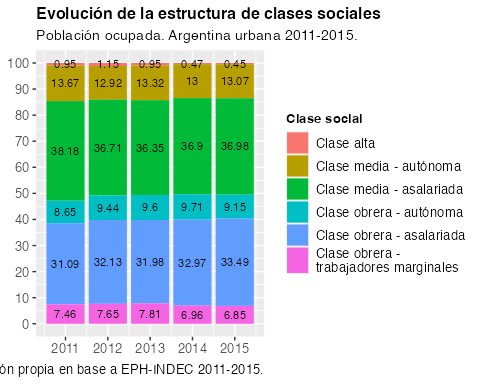
\includegraphics{docs_files/figure-latex/unnamed-chunk-123-1} 

}

\caption{Ejemplo de gráfico de columnas con la variable clase social}\label{fig:unnamed-chunk-123}
\end{figure}

\hypertarget{espacial}{%
\subsection{La dimensión espacial}\label{espacial}}

La dimensión espacial es otro de los elementos que todo estudio de la estructura social y de las clases sociales debería considerar. Como bien señala Osorio (\protect\hyperlink{ref-Osorio2001}{2001, p. 51}) ésta remite al vínculo sociedad-naturaleza, al clima y a las condiciones geográfico-naturales que desempeñan un papel fundamental en la historia. Naciones, provincias, departamentos y hasta ciudades condensan una serie de heterogeneidades en su interior y entre sí mismas, que obligan al investigador a considerarlas en su fase de análisis.

Claro está que no siempre contamos con las fuentes de información óptimas para abordar dicha heterogeneidades geográficas. Por ejemplo, con la \textbf{EPH}, fuente que venimos utilizando en este libro, podemos tener una desagregación espacial para el país por aglomerados, provincias o regiones, pero siempre considerando a la población urbana encuestada. Algo similar sucede con otras encuestas de hogares como la \href{https://www.argentina.gob.ar/ciencia/pisac/bases-de-datos}{ENES-PISAC}.

Por el contrario, la información censal nos permite acceder a un nivel de desagregación geo-estadísticas de mayor precisión, tales como las fracciones y los radios censales. De esta forma, el mosaico de heterogeneidades sociales que podemos representar se vuelve más complejo a través de este tipo de fuente de datos.

\hypertarget{algunos-ejemplos-de-la-bibliografuxeda-1}{%
\subsubsection{Algunos ejemplos de la bibliografía}\label{algunos-ejemplos-de-la-bibliografuxeda-1}}

Por limitaciones de las fuentes de información, en los estudios de estructuras de clases, cuando se cruzan los datos construidos con información espacial se suelen hacer comparaciones entre unidades de mayor nivel, tales como los países o las provincias y regiones dentro de las naciones. Por ejemplo, el análisis de Solís, Chávez Molina y Cobos (\protect\hyperlink{ref-Solis.etal2019}{2019}) se compara la estructura de clases reciente en 9 países latinoamericanos. Para ello se recurrió a información específica proveniente de encuestas de hogares de cada uno de los países seleccionados, que luego fue armonizada para poder ser comparable.

En Argentina, al igual que para el caso del análisis en el tiempo, los trabajos de Germani, Torrado también abordaron el análisis de la dinámica del cambio en la estructura de clases en agregados geográficos subnacionales.

Posteriormente, bajo la asesoría general de Susana Torrado, desde Consejo Nacional de Inversiones (\protect\hyperlink{ref-CFI1988}{CFI, 1988}), se elaboraron informes para cada una de las provincias y el total país, en donde se caracterizaba la estratificación social y las condiciones de vida de la población, teniendo como fuente de datos el Censo Nacional de Población y Vivienda de 1980. Gran parte de dicho análisis fue retomado luego y publicado en el libro \emph{Estructura social de la Argentina, 1945-1983} (\protect\hyperlink{ref-Torrado1992}{Torrado, 1992}).

Actualmente, con el avance y la difusión de la utilización de sistemas de información geográfica (SIG), se abrió la posibilidad de representación gráfica a través de mapas temáticos de información censal o proveniente de encuestas de hogares. Si bien aún en los estudios de estructura de clases no se ha tornado en una práctica frecuente, cada vez aparecen más trabajos que recurren a la representación geográfica de los datos para ilustrar los cambios y la evolución en la estructura social y de clases.

Por ejemplo, Mike Savage y otros (\protect\hyperlink{ref-Savage.etal2013}{2013}) llevaron a cabo junto a la BBC una encuesta de representación nacional (\emph{BBC's 2011 Great British Class Survey}), a través de la cual, a partir de la técnica de clases latentes, presentaron un nuevo abordaje en el estudio de las clases sociales conformado a partir de 7 clases. En ese trabajos, los autores recurren a una serie de mapas para demostrar cómo dichas clases se distribuyen al interior de Gran Bretaña.

\hypertarget{ejemplo-pruxe1ctico-1}{%
\subsubsection{Ejemplo práctico}\label{ejemplo-pruxe1ctico-1}}

Ahora veremos como llevar a cabo un análisis de clase según información espacial. Cómo dijimos anteriormente, la profundidad del tipo de análisis que podamos realizar va a depender del tipo de fuente con la que trabajemos. En este caso, vamos a aprovechar el pool de bases de \textbf{EPH} que hemos pegado para los años 2011 a 2015.

En forma simple vamos a indagar como se distribuyen las clases sociales al interior de cada una de las regiones identificadas por \textbf{INDEC}. En primer lugar, construyamos una tabla (no mostrada) de doble entrada que nos permita mostrar dicha información.

\begin{Shaded}
\begin{Highlighting}[]
\CommentTok{\# 1) Creo una variable factor con los nombres de las regiones (region\_f)}
\NormalTok{eph\_1115\_ocup}\SpecialCharTok{$}\NormalTok{region\_f }\OtherTok{\textless{}{-}} \FunctionTok{factor}\NormalTok{(eph\_1115\_ocup}\SpecialCharTok{$}\NormalTok{REGION, }\AttributeTok{labels =} \FunctionTok{c}\NormalTok{(}\StringTok{"GBA"}\NormalTok{, }\StringTok{"NOA"}\NormalTok{, }\StringTok{"NEA"}\NormalTok{,}
    \StringTok{"Cuyo"}\NormalTok{, }\StringTok{"Pampeana"}\NormalTok{, }\StringTok{"Patagonia"}\NormalTok{))}

\CommentTok{\# 2) Construimos un objeto tabla cruzando la variable clase6\_factor y region\_f}
\NormalTok{tabla\_regiones }\OtherTok{\textless{}{-}}\NormalTok{ eph\_1115\_ocup }\SpecialCharTok{\%\textgreater{}\%}
    \FunctionTok{filter}\NormalTok{(}\SpecialCharTok{!}\FunctionTok{is.na}\NormalTok{(clase6\_factor)) }\SpecialCharTok{\%\textgreater{}\%}
    \FunctionTok{group\_by}\NormalTok{(region\_f, clase6\_factor) }\SpecialCharTok{\%\textgreater{}\%}
    \FunctionTok{tally}\NormalTok{(}\AttributeTok{wt =}\NormalTok{ PONDERA) }\SpecialCharTok{\%\textgreater{}\%}
    \FunctionTok{group\_by}\NormalTok{(region\_f) }\SpecialCharTok{\%\textgreater{}\%}
    \FunctionTok{mutate}\NormalTok{(}\AttributeTok{percent =} \FunctionTok{round}\NormalTok{((n}\SpecialCharTok{/}\FunctionTok{sum}\NormalTok{(n)) }\SpecialCharTok{*} \DecValTok{100}\NormalTok{, }\AttributeTok{digits =} \DecValTok{2}\NormalTok{)) }\SpecialCharTok{\%\textgreater{}\%}
    \FunctionTok{select}\NormalTok{(clase6\_factor, region\_f, percent) }\SpecialCharTok{\%\textgreater{}\%}
    \FunctionTok{spread}\NormalTok{(region\_f, }\AttributeTok{value =}\NormalTok{ percent)}
\end{Highlighting}
\end{Shaded}

Finalmente presentamos un ejemplo de representación de la tabla anteriormente construida en un mapa temático. \textbf{\texttt{R}} posee varias librerías para manipular información de tipo geográfica. En este caso utilizaremos el paquete \texttt{sf}. Lo que haremos es representar en mapas en miniatura de Argentina, el porcentaje de individuos pertenecientes a cada clase social por región.

A los fines de este ejemplo, trabajaremos con la cartografía por departamentos que proporciona INDEC (\url{https://www.indec.gob.ar/indec/web/Institucional-Indec-Codgeo}). Si bien no es la finalidad de este libro introducir el uso de herramientas SIG\footnote{Recomendamos el manual \href{https://bitsandbricks.github.io/ciencia_de_datos_gente_sociable/}{Ciencia de datos para gente sociable}, específicamente su capítulo 6, para quienes quieran profundizar en el tema}, a continuación presentamos el procedimiento ``paso a paso'' para la creación del mapa temático.

\begin{Shaded}
\begin{Highlighting}[]
\CommentTok{\# 1) Cargamos el archivo .shp y lo guardamos en el objetivo espacial}
\CommentTok{\# \textquotesingle{}argentina\textquotesingle{}}
\NormalTok{argentina }\OtherTok{\textless{}{-}} \FunctionTok{st\_read}\NormalTok{(}\StringTok{"cartografia/argentina\_n.shp"}\NormalTok{)}
\end{Highlighting}
\end{Shaded}

\begin{verbatim}
Reading layer `argentina_n' from data source 
  `/Users/nxs851/GitHub/academia/teaching/UNTreF/clases-arg/cartografia/argentina_n.shp' 
  using driver `ESRI Shapefile'
Simple feature collection with 1242 features and 10 fields
Geometry type: POLYGON
Dimension:     XY
Bounding box:  xmin: -74 ymin: -90 xmax: -25 ymax: -22
Geodetic CRS:  WGS 84
\end{verbatim}

\begin{Shaded}
\begin{Highlighting}[]
\CommentTok{\# 2) Filtramos al territorio antártico ya que no contamos con información en la}
\CommentTok{\# EPH y se dificulta la visualización del mapa}
\NormalTok{argentina }\OtherTok{\textless{}{-}}\NormalTok{ argentina }\SpecialCharTok{\%\textgreater{}\%}
    \FunctionTok{filter}\NormalTok{(}\SpecialCharTok{!}\NormalTok{link }\SpecialCharTok{\%in\%} \FunctionTok{c}\NormalTok{(}\StringTok{"94028"}\NormalTok{))}

\CommentTok{\# provincias \textless{}{-}}
\CommentTok{\# st\_read(\textquotesingle{}E:/OneDrive/Otros/proyectos\_R/mapas/Codgeo\_Pais\_x\_prov\_datos/provincias\_n.shp\textquotesingle{})}

\CommentTok{\# 3) Creamos un vector con los 31 códigos geográficos de los 31 partidos del}
\CommentTok{\# GBA}
\NormalTok{partidos }\OtherTok{\textless{}{-}} \FunctionTok{c}\NormalTok{(}\StringTok{"06028"}\NormalTok{, }\StringTok{"06035"}\NormalTok{, }\StringTok{"06091"}\NormalTok{, }\StringTok{"06134"}\NormalTok{, }\StringTok{"06252"}\NormalTok{, }\StringTok{"06260"}\NormalTok{, }\StringTok{"06270"}\NormalTok{, }\StringTok{"06274"}\NormalTok{,}
    \StringTok{"06364"}\NormalTok{, }\StringTok{"06371"}\NormalTok{, }\StringTok{"06408"}\NormalTok{, }\StringTok{"06410"}\NormalTok{, }\StringTok{"06412"}\NormalTok{, }\StringTok{"06427"}\NormalTok{, }\StringTok{"06434"}\NormalTok{, }\StringTok{"06490"}\NormalTok{, }\StringTok{"06515"}\NormalTok{,}
    \StringTok{"06525"}\NormalTok{, }\StringTok{"06539"}\NormalTok{, }\StringTok{"06560"}\NormalTok{, }\StringTok{"06568"}\NormalTok{, }\StringTok{"06638"}\NormalTok{, }\StringTok{"06648"}\NormalTok{, }\StringTok{"06658"}\NormalTok{, }\StringTok{"06749"}\NormalTok{, }\StringTok{"06756"}\NormalTok{,}
    \StringTok{"06760"}\NormalTok{, }\StringTok{"06778"}\NormalTok{, }\StringTok{"06805"}\NormalTok{, }\StringTok{"06840"}\NormalTok{, }\StringTok{"06861"}\NormalTok{)}

\CommentTok{\# 4) Definimos dentro del objeto geográfico \textquotesingle{}argentina\textquotesingle{} a la columna link como}
\CommentTok{\# caracter y a la columna codpcia como numérica}
\NormalTok{argentina}\SpecialCharTok{$}\NormalTok{link }\OtherTok{\textless{}{-}} \FunctionTok{as.character}\NormalTok{(argentina}\SpecialCharTok{$}\NormalTok{link)}
\NormalTok{argentina}\SpecialCharTok{$}\NormalTok{codpcia }\OtherTok{\textless{}{-}} \FunctionTok{as.numeric}\NormalTok{(argentina}\SpecialCharTok{$}\NormalTok{codpcia)}

\CommentTok{\# 5) Creamos en el objeto \textquotesingle{}argentina\textquotesingle{} una variable llamada REGION que agrupe a}
\CommentTok{\# las provincias igual que en la EPH}
\NormalTok{argentina }\OtherTok{\textless{}{-}}\NormalTok{ argentina }\SpecialCharTok{\%\textgreater{}\%}
    \FunctionTok{mutate}\NormalTok{(}\AttributeTok{region\_f =} \FunctionTok{case\_when}\NormalTok{(codpcia }\SpecialCharTok{==} \DecValTok{2} \SpecialCharTok{|}\NormalTok{ (link }\SpecialCharTok{\%in\%}\NormalTok{ partidos) }\SpecialCharTok{\textasciitilde{}} \StringTok{"GBA"}\NormalTok{, codpcia }\SpecialCharTok{==}
        \DecValTok{10} \SpecialCharTok{|}\NormalTok{ codpcia }\SpecialCharTok{==} \DecValTok{38} \SpecialCharTok{|}\NormalTok{ codpcia }\SpecialCharTok{==} \DecValTok{46} \SpecialCharTok{|}\NormalTok{ codpcia }\SpecialCharTok{==} \DecValTok{66} \SpecialCharTok{|}\NormalTok{ codpcia }\SpecialCharTok{==} \DecValTok{90} \SpecialCharTok{|}\NormalTok{ codpcia }\SpecialCharTok{==}
        \DecValTok{86} \SpecialCharTok{\textasciitilde{}} \StringTok{"NOA"}\NormalTok{, codpcia }\SpecialCharTok{==} \DecValTok{18} \SpecialCharTok{|}\NormalTok{ codpcia }\SpecialCharTok{==} \DecValTok{22} \SpecialCharTok{|}\NormalTok{ codpcia }\SpecialCharTok{==} \DecValTok{54} \SpecialCharTok{|}\NormalTok{ codpcia }\SpecialCharTok{==} \DecValTok{34} \SpecialCharTok{\textasciitilde{}}
        \StringTok{"NEA"}\NormalTok{, codpcia }\SpecialCharTok{==} \DecValTok{50} \SpecialCharTok{|}\NormalTok{ codpcia }\SpecialCharTok{==} \DecValTok{70} \SpecialCharTok{|}\NormalTok{ codpcia }\SpecialCharTok{==} \DecValTok{74} \SpecialCharTok{\textasciitilde{}} \StringTok{"Cuyo"}\NormalTok{, (codpcia }\SpecialCharTok{==}
        \DecValTok{6} \SpecialCharTok{\&} \SpecialCharTok{!}\NormalTok{(link }\SpecialCharTok{\%in\%}\NormalTok{ partidos)) }\SpecialCharTok{|}\NormalTok{ codpcia }\SpecialCharTok{==} \DecValTok{30} \SpecialCharTok{|}\NormalTok{ codpcia }\SpecialCharTok{==} \DecValTok{14} \SpecialCharTok{|}\NormalTok{ codpcia }\SpecialCharTok{==} \DecValTok{82} \SpecialCharTok{|}
\NormalTok{        codpcia }\SpecialCharTok{==} \DecValTok{42} \SpecialCharTok{\textasciitilde{}} \StringTok{"Pampeana"}\NormalTok{, codpcia }\SpecialCharTok{==} \DecValTok{58} \SpecialCharTok{|}\NormalTok{ codpcia }\SpecialCharTok{==} \DecValTok{62} \SpecialCharTok{|}\NormalTok{ codpcia }\SpecialCharTok{==} \DecValTok{26} \SpecialCharTok{|}
\NormalTok{        codpcia }\SpecialCharTok{==} \DecValTok{78} \SpecialCharTok{|}\NormalTok{ codpcia }\SpecialCharTok{==} \DecValTok{94} \SpecialCharTok{\textasciitilde{}} \StringTok{"Patagonia"}\NormalTok{))}

\CommentTok{\# 6) Volvemos a crear una tabla con los porcentajes de individuos por clase}
\CommentTok{\# sociales según región, pero esta vez en formato largo}

\NormalTok{tabla\_larga }\OtherTok{\textless{}{-}}\NormalTok{ eph\_1115\_ocup }\SpecialCharTok{\%\textgreater{}\%}
    \FunctionTok{filter}\NormalTok{(}\SpecialCharTok{!}\FunctionTok{is.na}\NormalTok{(clase6\_factor)) }\SpecialCharTok{\%\textgreater{}\%}
    \FunctionTok{group\_by}\NormalTok{(region\_f, clase6\_factor) }\SpecialCharTok{\%\textgreater{}\%}
    \FunctionTok{tally}\NormalTok{(}\AttributeTok{wt =}\NormalTok{ PONDERA) }\SpecialCharTok{\%\textgreater{}\%}
    \FunctionTok{group\_by}\NormalTok{(region\_f) }\SpecialCharTok{\%\textgreater{}\%}
    \FunctionTok{mutate}\NormalTok{(}\AttributeTok{percent =} \FunctionTok{round}\NormalTok{((n}\SpecialCharTok{/}\FunctionTok{sum}\NormalTok{(n)) }\SpecialCharTok{*} \DecValTok{100}\NormalTok{, }\AttributeTok{digits =} \DecValTok{2}\NormalTok{))}

\CommentTok{\# 7) Unimos el objeto \textquotesingle{}argentina\textquotesingle{} con la tabla larga que contiene los}
\CommentTok{\# porcentajes por clase y región, tomando como variable identificadora REGION}
\NormalTok{mapa }\OtherTok{\textless{}{-}} \FunctionTok{merge}\NormalTok{(argentina, tabla\_larga, }\AttributeTok{by =} \StringTok{"region\_f"}\NormalTok{, }\AttributeTok{all.x =} \ConstantTok{TRUE}\NormalTok{)}
\end{Highlighting}
\end{Shaded}

Puntualmente, el comando \texttt{geom\_sf} del \texttt{ggplot2} nos permitirá superponer capas con información georreferenciada, como en este caso los departamentos del país. A su vez, el comando \texttt{facet\_wrap} del mismo paquete nos permite representar un gráfico (en este caso un mapa) para la variable que seleccionemos (clase social).

\begin{Shaded}
\begin{Highlighting}[]
\FunctionTok{ggplot}\NormalTok{() }\SpecialCharTok{+}
  \FunctionTok{geom\_sf}\NormalTok{(}\AttributeTok{data =}\NormalTok{ mapa, }\FunctionTok{aes}\NormalTok{(}\AttributeTok{group =}\NormalTok{ region\_f, }\AttributeTok{fill =}\NormalTok{ percent), }\AttributeTok{color =} \ConstantTok{NA}\NormalTok{) }\SpecialCharTok{+}
  \FunctionTok{theme\_map}\NormalTok{() }\SpecialCharTok{+}
  \FunctionTok{labs}\NormalTok{(}\AttributeTok{fill =} \StringTok{"\% Clase social"}\NormalTok{,}
       \AttributeTok{title =} \StringTok{"Distribución de las clases sociales por región"}\NormalTok{,}
       \AttributeTok{subtitle =} \StringTok{"Población ocupada. Argentina urbana 2011{-}2015."}\NormalTok{,}
       \AttributeTok{caption =} \StringTok{"Fuente: Elaboración propia en base a EPH{-}INDEC 2011{-}2015."}\NormalTok{) }\SpecialCharTok{+}
  \FunctionTok{theme}\NormalTok{(}\AttributeTok{legend.title =} \FunctionTok{element\_text}\NormalTok{(}\AttributeTok{size =} \DecValTok{10}\NormalTok{, }\AttributeTok{face =} \StringTok{"bold"}\NormalTok{),}
        \AttributeTok{legend.text =} \FunctionTok{element\_text}\NormalTok{(}\AttributeTok{size =} \DecValTok{9}\NormalTok{),}
        \AttributeTok{legend.key.width =} \FunctionTok{unit}\NormalTok{(}\FloatTok{1.5}\NormalTok{, }\StringTok{"cm"}\NormalTok{),}
        \AttributeTok{legend.position =} \StringTok{"bottom"}\NormalTok{,}
        \AttributeTok{legend.justification =} \StringTok{"center"}\NormalTok{,}
        \AttributeTok{plot.title =} \FunctionTok{element\_text}\NormalTok{(}\AttributeTok{size =} \DecValTok{12}\NormalTok{, }\AttributeTok{face =} \StringTok{"bold"}\NormalTok{),}
        \AttributeTok{plot.subtitle =} \FunctionTok{element\_text}\NormalTok{(}\AttributeTok{size =} \DecValTok{11}\NormalTok{),}
        \AttributeTok{plot.caption =} \FunctionTok{element\_text}\NormalTok{(}\AttributeTok{size =} \DecValTok{10}\NormalTok{, }\AttributeTok{hjust =} \DecValTok{1}\NormalTok{),}
        \AttributeTok{strip.text =} \FunctionTok{element\_text}\NormalTok{(}\AttributeTok{face =} \StringTok{"bold"}\NormalTok{, }\AttributeTok{size =} \DecValTok{10}\NormalTok{)) }\SpecialCharTok{+}
  \FunctionTok{scale\_fill\_viridis\_c}\NormalTok{(}\AttributeTok{direction =} \SpecialCharTok{{-}}\DecValTok{1}\NormalTok{) }\SpecialCharTok{+}
  \FunctionTok{facet\_wrap}\NormalTok{(}\SpecialCharTok{\textasciitilde{}}\NormalTok{clase6\_factor, }\AttributeTok{ncol =} \DecValTok{7}\NormalTok{, }\AttributeTok{labeller =} \FunctionTok{labeller}\NormalTok{(}\AttributeTok{clase6\_factor =} \FunctionTok{label\_wrap\_gen}\NormalTok{(}\DecValTok{15}\NormalTok{)))}
\end{Highlighting}
\end{Shaded}

\begin{figure}

{\centering 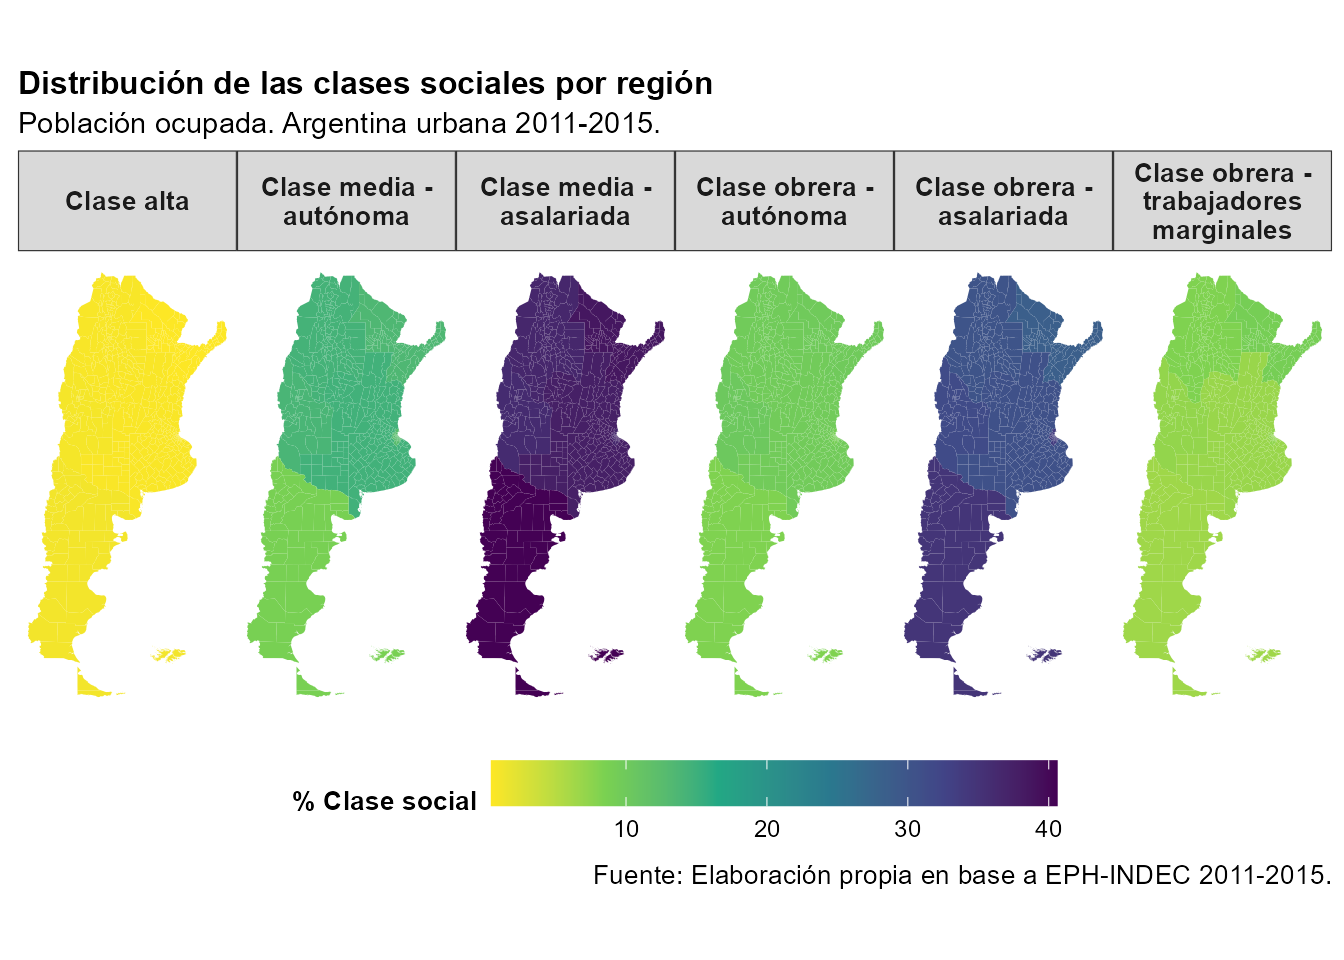
\includegraphics{docs_files/figure-latex/unnamed-chunk-132-1} 

}

\caption{Ejemplo de mapa temático utilizando la variable clase social}\label{fig:unnamed-chunk-132}
\end{figure}

\hypertarget{part-anexo}{%
\part{Anexo}\label{part-anexo}}

\hypertarget{anexo}{%
\section{Introducción a R y RStudio}\label{anexo}}

La mayor parte de los ejercicios expuestos a lo largo de este Manual utilizan una o más funciones de \textbf{\texttt{R}} para resolver un problema específico. Se destaca que no se describen las funciones en detalle, ya que ellas pueden ser consultadas en otras publicaciones. Sin embargo, en este anexo, se presenta una introducción básica a la programación en \texttt{R} con \texttt{RStudio} y una selección de recursos disponibles para profundizar en su práctica.

\hypertarget{introR}{%
\subsection{Introducción}\label{introR}}

\textbf{\texttt{R}} es un lenguaje de programación usado para realizar análisis estadístico y en general, análisis de datos. Se trata de un conjunto integrado de programas para trabajar con datos, cálculos y gráficos, que permite:

\begin{itemize}
\item
  almacenar y manipular datos,
\item
  operar cálculos sobre variables indexadas (como las matrices),
\item
  analizar datos con una colección de herramientas,
\item
  aplicar herramientas gráficas para el análisis de datos y,
\item
  programar con un lenguaje sencillo y en constante desarrollo.
\end{itemize}

\textbf{\texttt{R}} es el lenguaje de programación popular debido a tres ventajas principales:

\begin{itemize}
\item
  \textbf{accesibilidad}: cualquiera puede descargar el programa de manera gratuita,
\item
  \textbf{código abierto}: quien desee modificar el código de \textbf{\texttt{R}}, puede hacerlo, y
\item
  \textbf{comunidad de usuarios}: existe una actividad permanente alrededor de \textbf{\texttt{R}}, que brinda soporte a los usuarios para resolver dudas y aprender en línea.
\end{itemize}

\hypertarget{el-entorno-de-r}{%
\subsubsection{El entorno de R}\label{el-entorno-de-r}}

\begin{itemize}
\item
  \textbf{\texttt{R}} se puede entender como el entorno donde se implementan múltiples técnicas estadísticas. El concepto de ``entorno'' se refiere a que es un sistema diseñado específicamente para el análisis de datos, que posee coherencia interna y que es más que el agregado de cada una de las herramientas que lo conforman.
\item
  Gracias a la implementación de \textbf{\texttt{R}} se han desarrollado numerosos métodos interactivos para analizar datos. Los usuarios de \textbf{\texttt{R}} se han ido \emph{aggiornando} con cada versión del programa que ha salido, añadiendo métodos que acompañan las nuevas tecnologías.
\end{itemize}

\hypertarget{aplicar-estaduxedstica-en-r}{%
\subsubsection{Aplicar estadística en R}\label{aplicar-estaduxedstica-en-r}}

\begin{itemize}
\item
  El entorno de \textbf{\texttt{R}} permite desplegar técnicas estadísticas, de las más antiguas hasta la más actuales. Esta ventaja no es proporcional al esfuerzo que implica buscar las herramientas del programa que permiten su aplicación.
\item
  Lo que diferencia a \textbf{\texttt{R}} de otros sistemas de análisis estadísticos como \textbf{Stata} o \textbf{SPSS} es que el \texttt{output} que se genera es escueto comparado con la cantidad de comandos (o \texttt{input}) que se deben imprimir para obtenerlo. Cada uno de los pasos a seguir se van almacenando en forma de \texttt{objetos}, que quedan disponibles para la observación y el análisis del usuario.
\item
  Algunas técnicas estadísticas están incluidas en el entorno básico de \textbf{\texttt{R}} y otras se pueden obtener en forma de bibliotecas, llamadas \textbf{paquetes} (\texttt{packages}).
\end{itemize}

\begin{figure}

{\centering 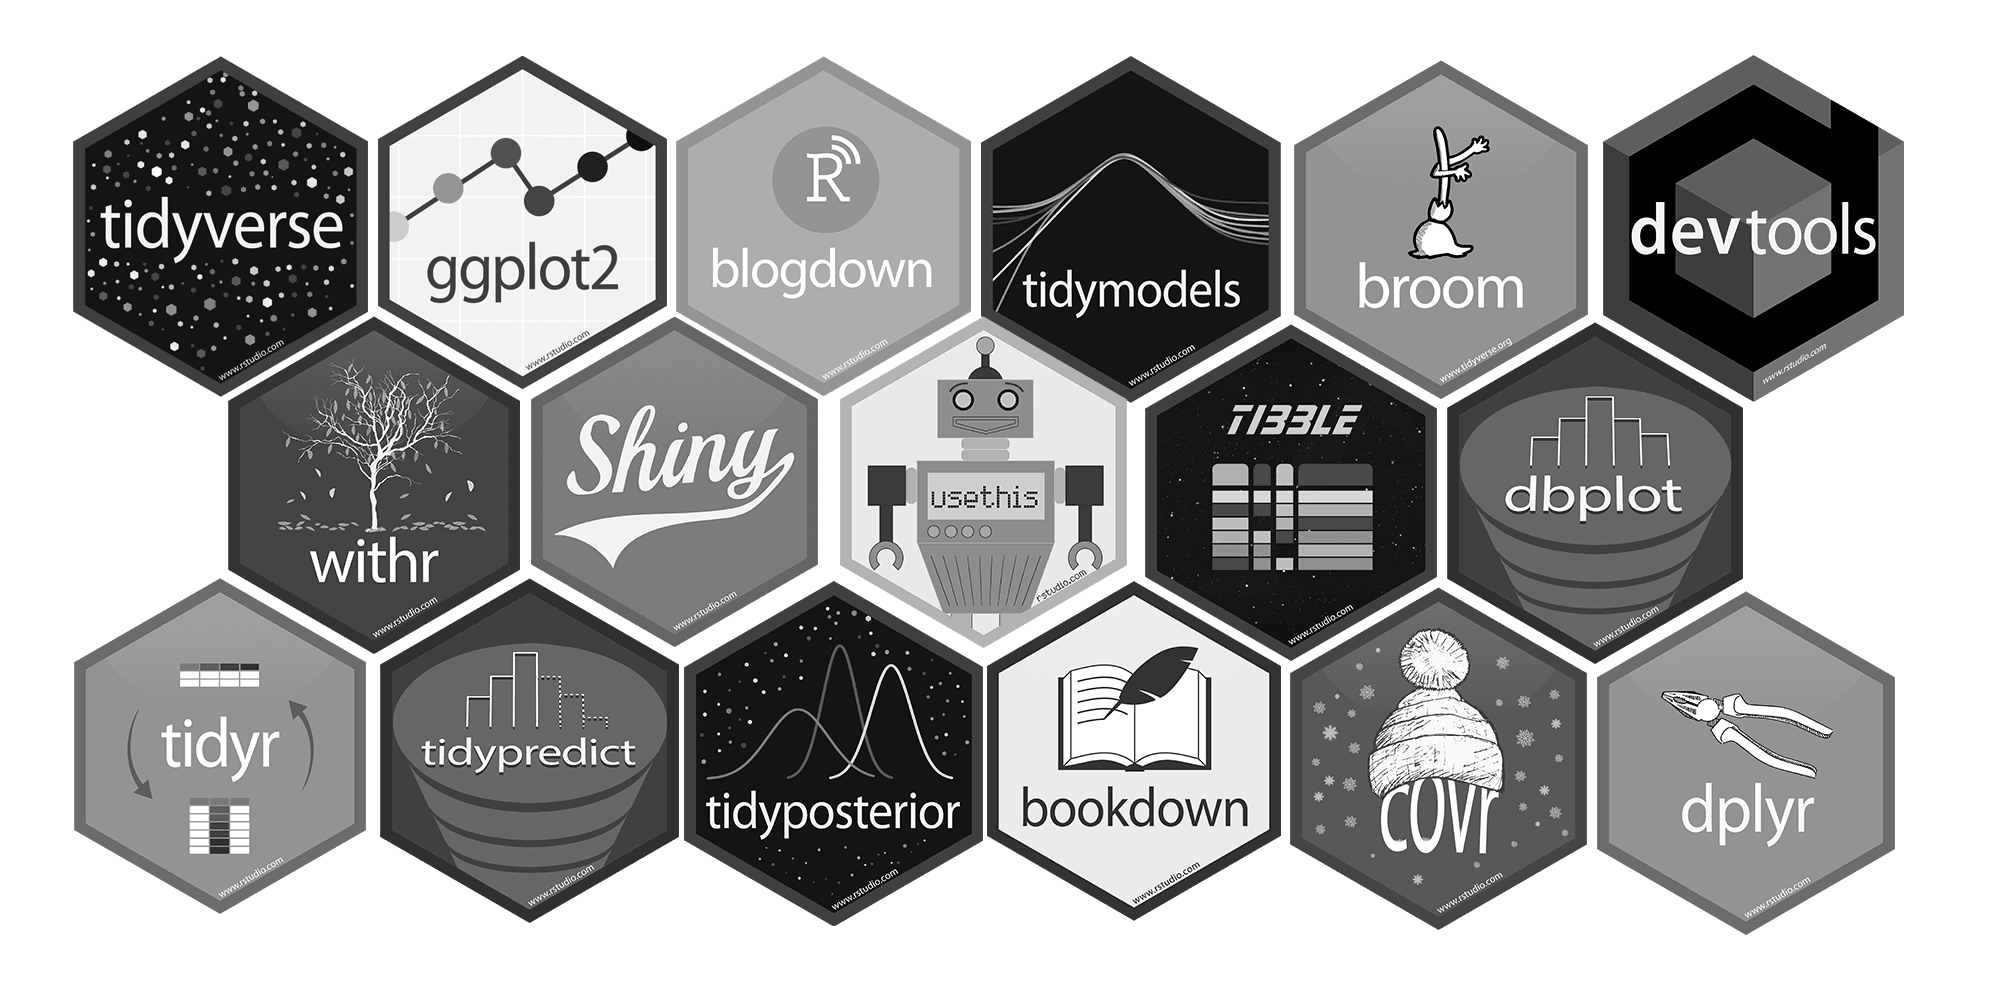
\includegraphics[width=0.6\linewidth]{imagenes/R_packages} 

}

\caption{Logos de algunos paquetes de R}\label{fig:unnamed-chunk-135}
\end{figure}

\hypertarget{descargar-e-instalar-r}{%
\subsubsection{Descargar e instalar R}\label{descargar-e-instalar-r}}

Para descargar \textbf{\texttt{R}} es posible ingresar a \url{https://cran.r-project.org/}. Luego, se debe seleccionar el sistema operativo de cada computadora donde se lo desea instalar y, a consiguiente, comenzará la instalación.

\begin{figure}

{\centering 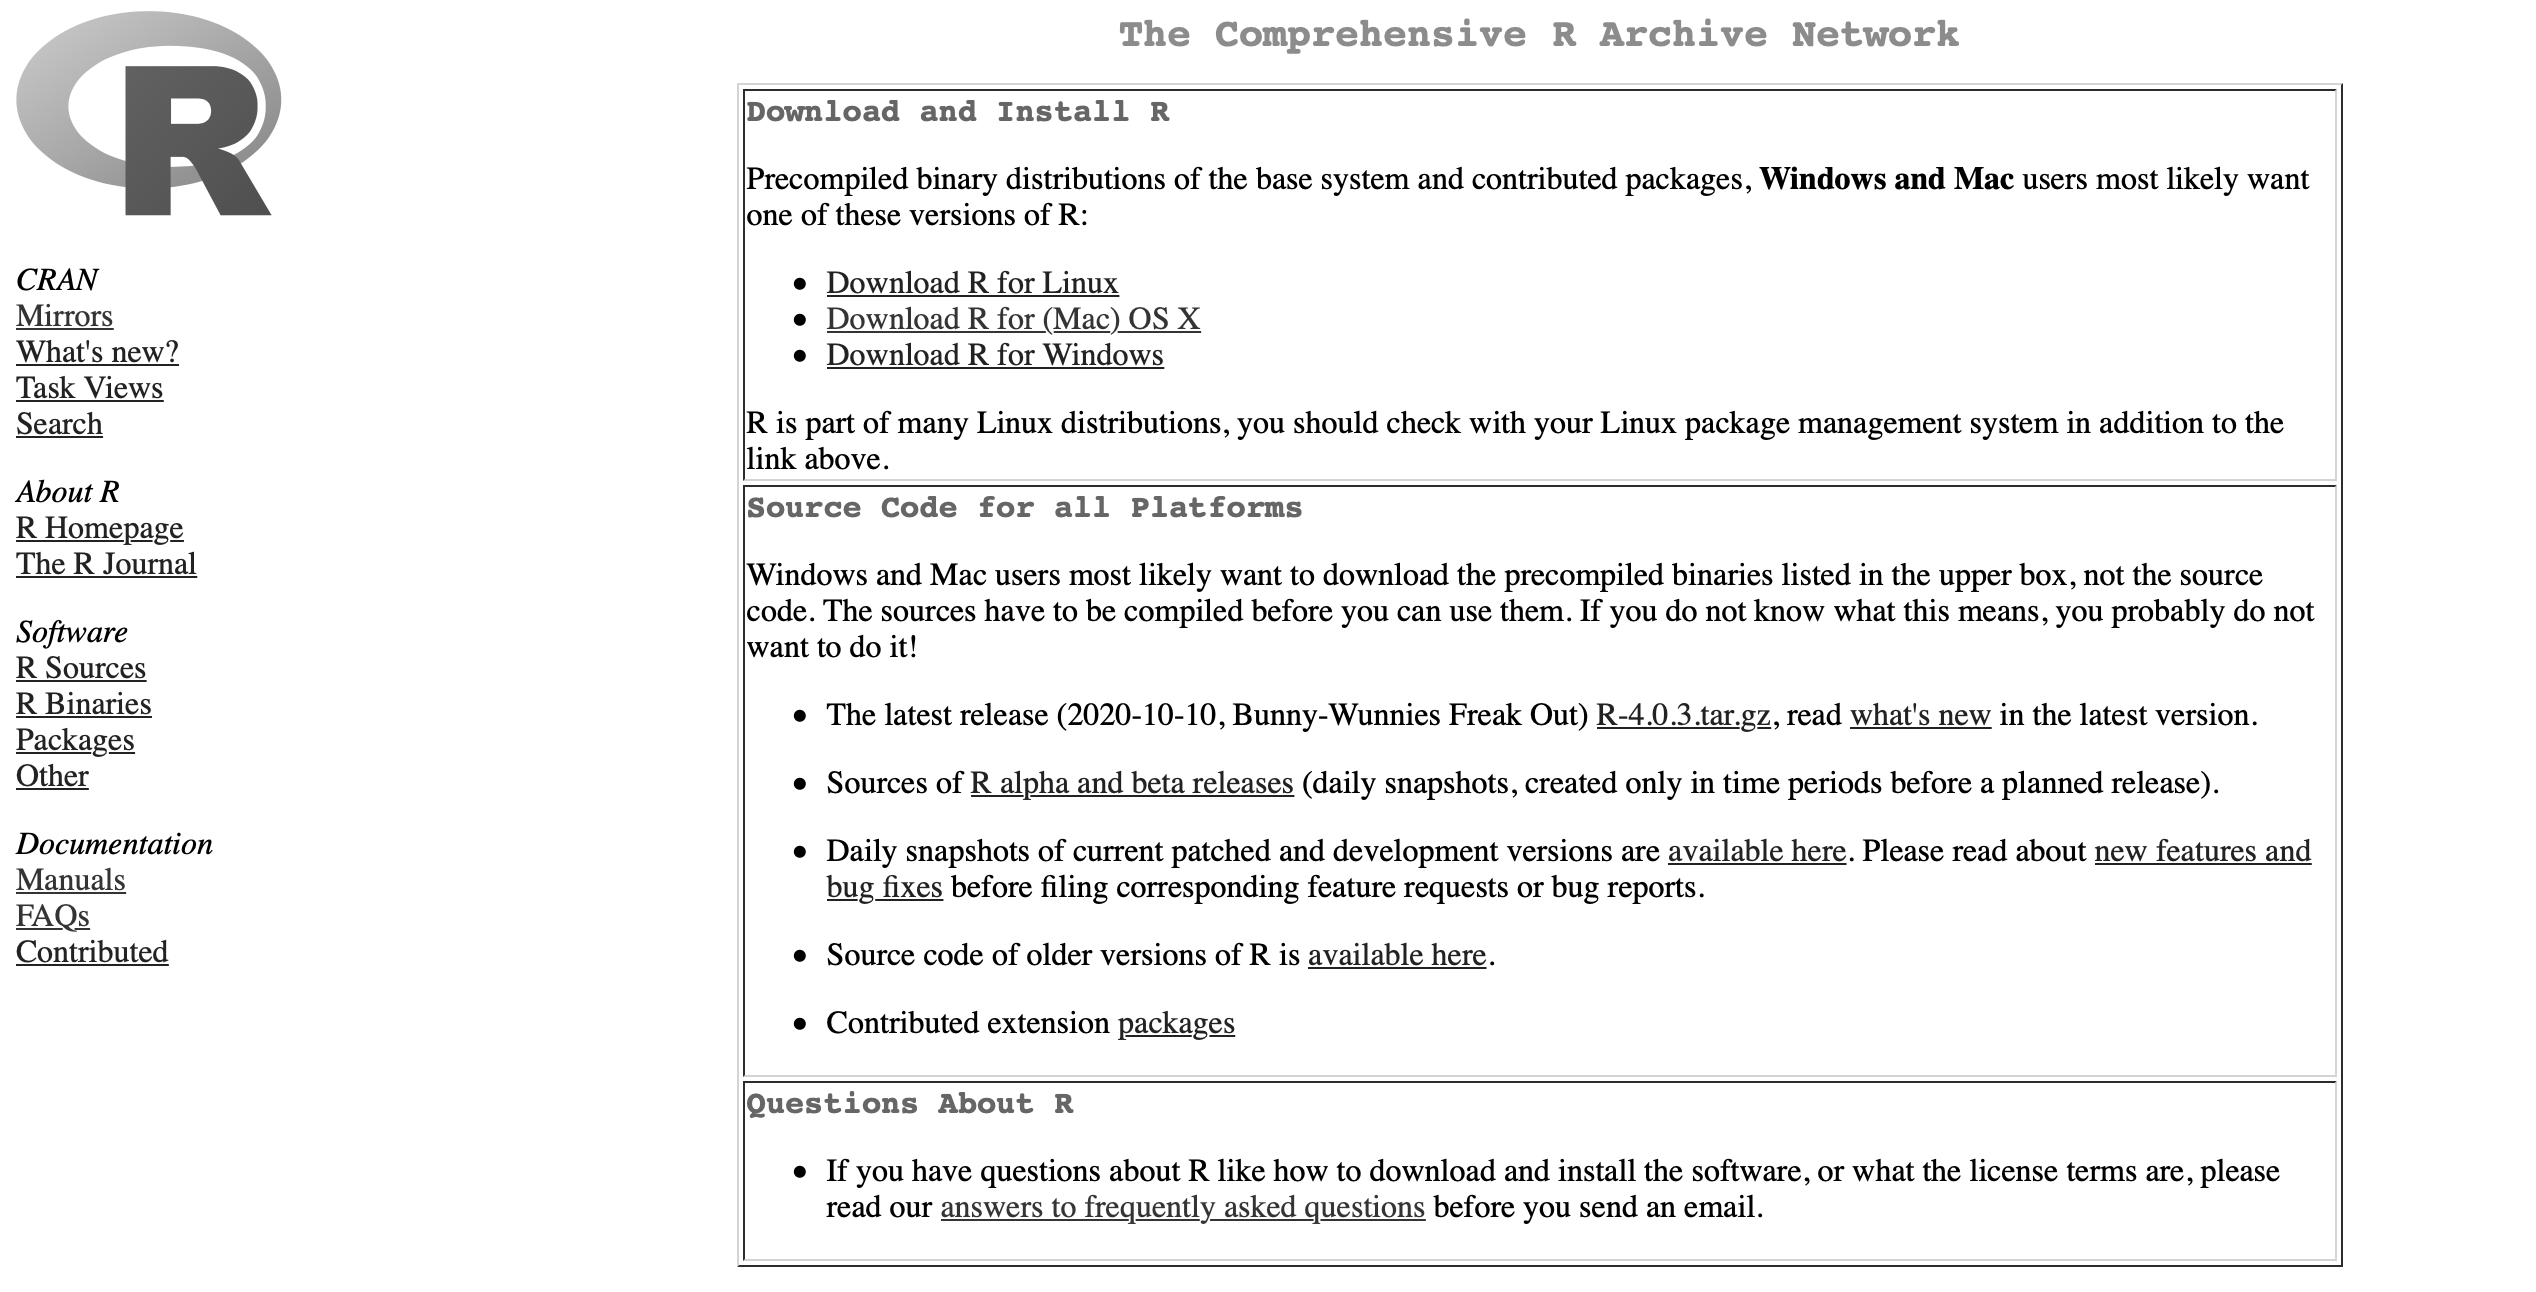
\includegraphics[width=0.8\linewidth]{imagenes/R_desc} 

}

\caption{R}\label{fig:unnamed-chunk-136}
\end{figure}

\hypertarget{rstudio}{%
\subsubsection{RStudio}\label{rstudio}}

\textbf{\texttt{RStudio}} es un \textbf{entorno de desarrollo integrado} (IDE, en inglés), que significa que contiene todas las herramientas que se necesitan en un mismo lugar. Las maneras más sencilla de ``comunicarse'' con \textbf{\texttt{R}} son:

\begin{itemize}
\item
  escribiendo líneas de comandos que conforman el código en la terminal o bien,
\item
  utilizando \texttt{RStudio}, que hace más atractiva y fácil la aproximación al programa.
\end{itemize}

\hypertarget{descargar-e-instalar-rstudio}{%
\subsubsection{Descargar e instalar RStudio}\label{descargar-e-instalar-rstudio}}

Se debe ingresar al siguiente enlace: \url{https://www.rstudio.com/products/rstudio/download/}

\begin{figure}

{\centering 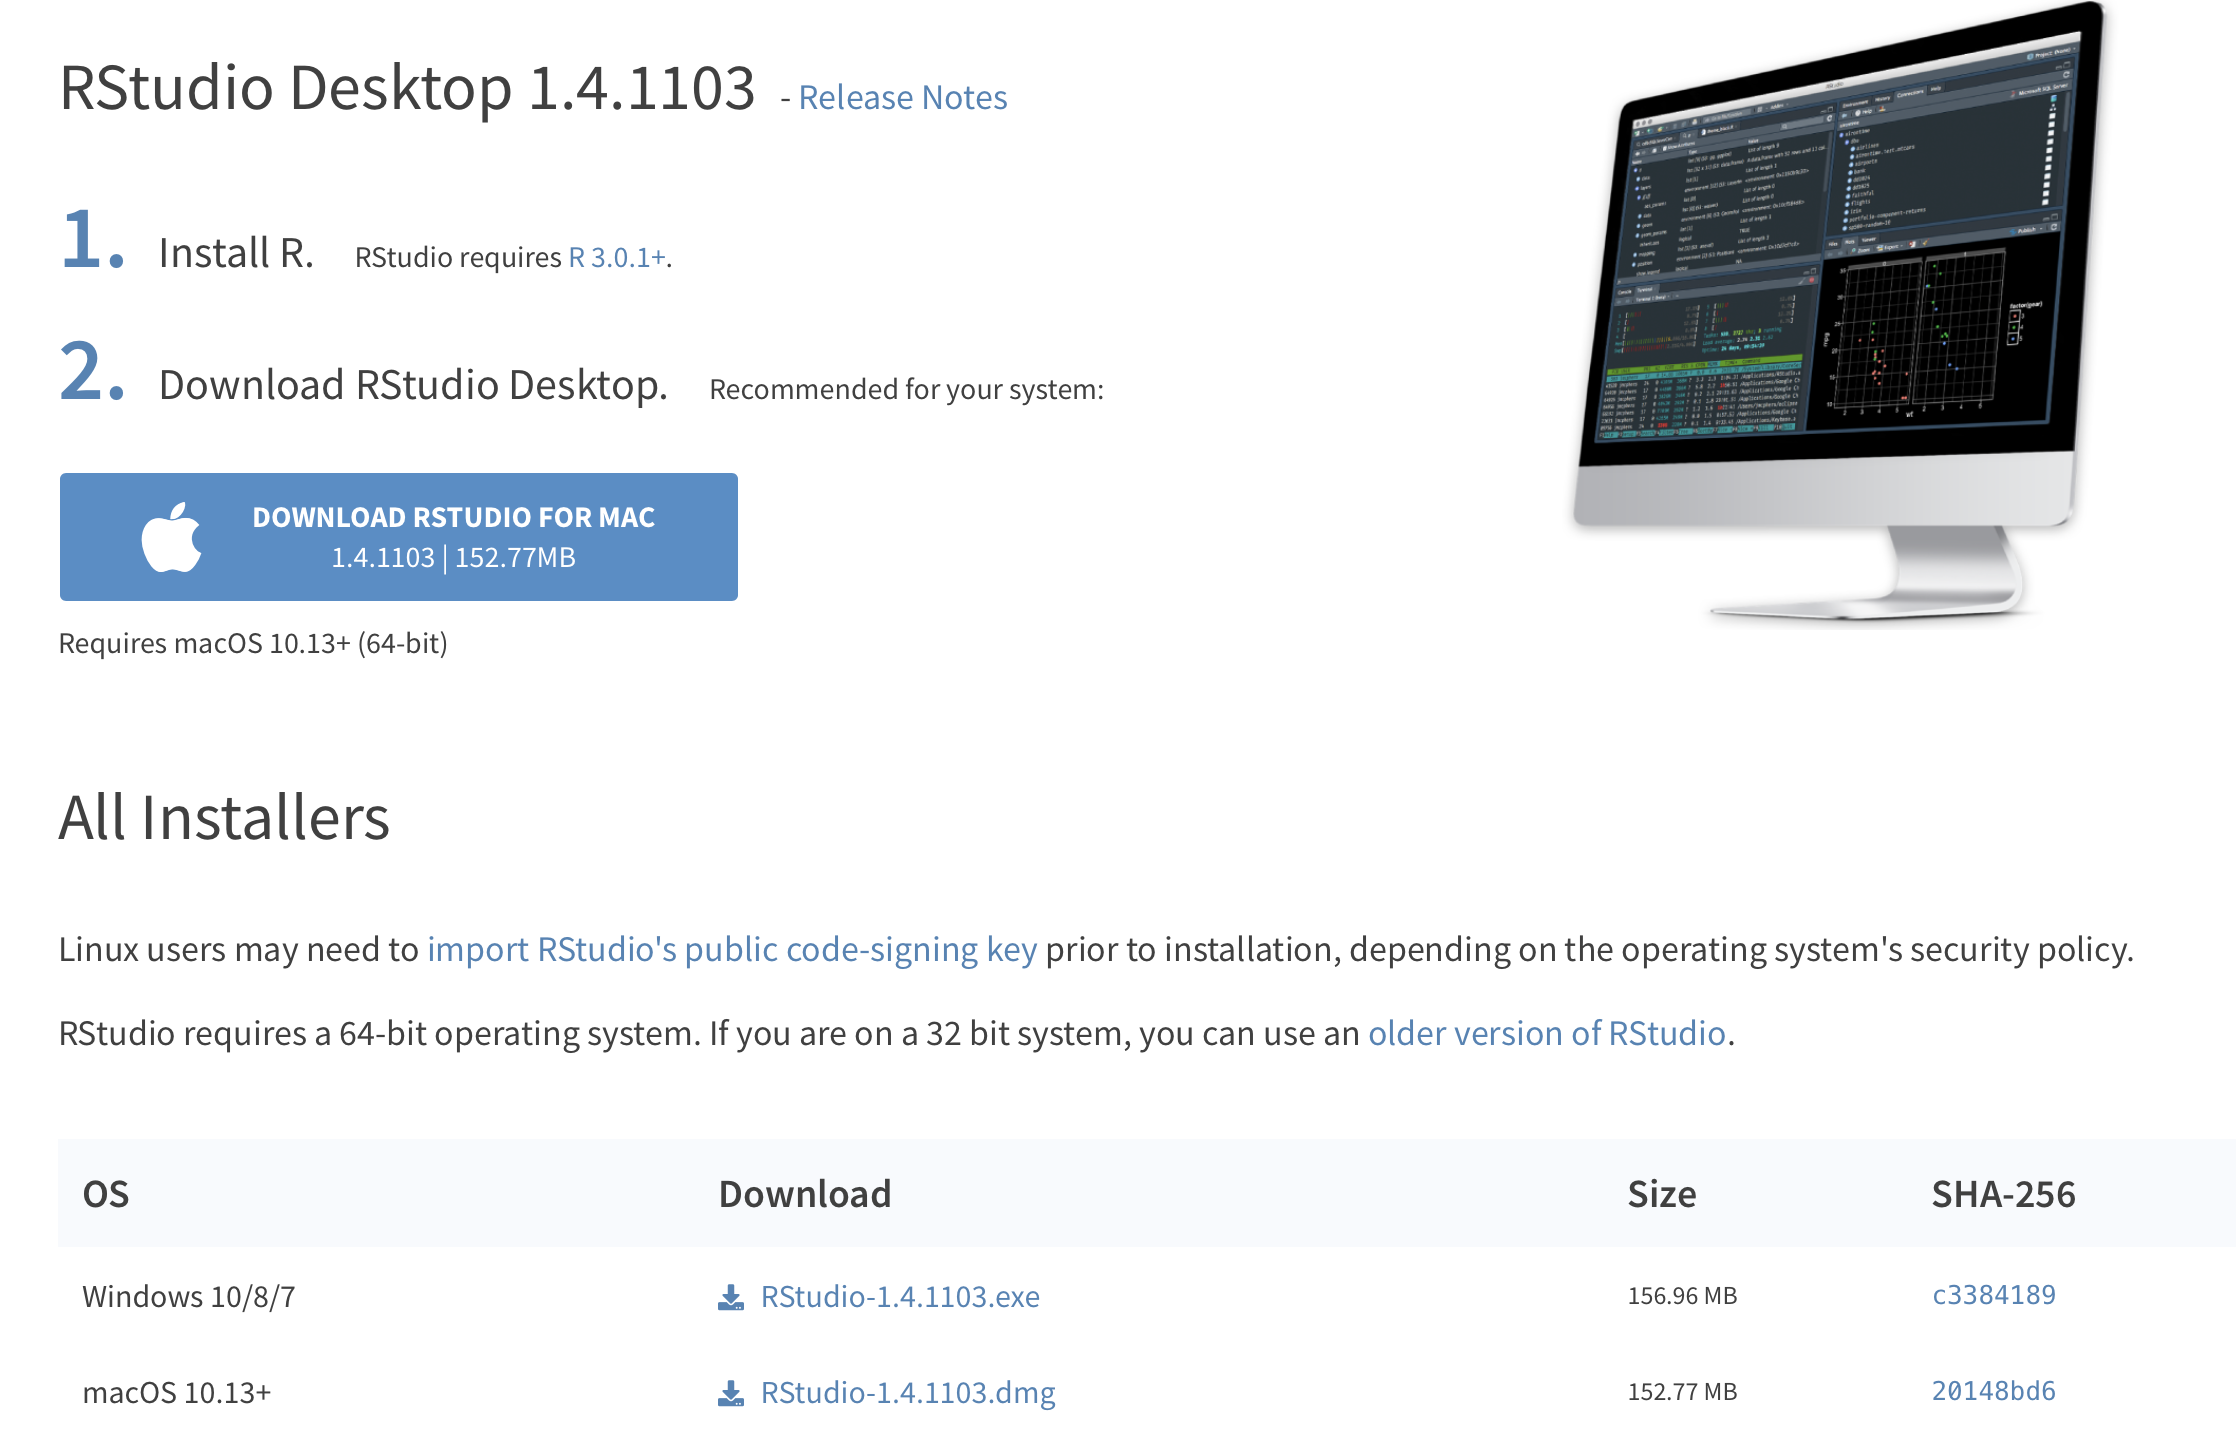
\includegraphics[width=0.8\linewidth]{imagenes/RStudio_desc} 

}

\caption{Descarga de RStudio}\label{fig:unnamed-chunk-138}
\end{figure}

\hypertarget{partes-de-rstudio}{%
\subsubsection{Partes de RStudio}\label{partes-de-rstudio}}

Las secciones que conforman \texttt{RStudio} son cuatro:

\begin{itemize}
\item
  la fuente (en la parte superior izquierda),
\item
  el entorno (parte superior derecha),
\item
  la consola (parte inferior izquierda) y
\item
  la sección de ``documentos, gráficos, paquetes y ayuda'' (parte inferior derecha).
\end{itemize}

Cuando uno abre \texttt{RStudio}, de forma predeterminada, se ve de la siguiente manera:

\begin{figure}

{\centering 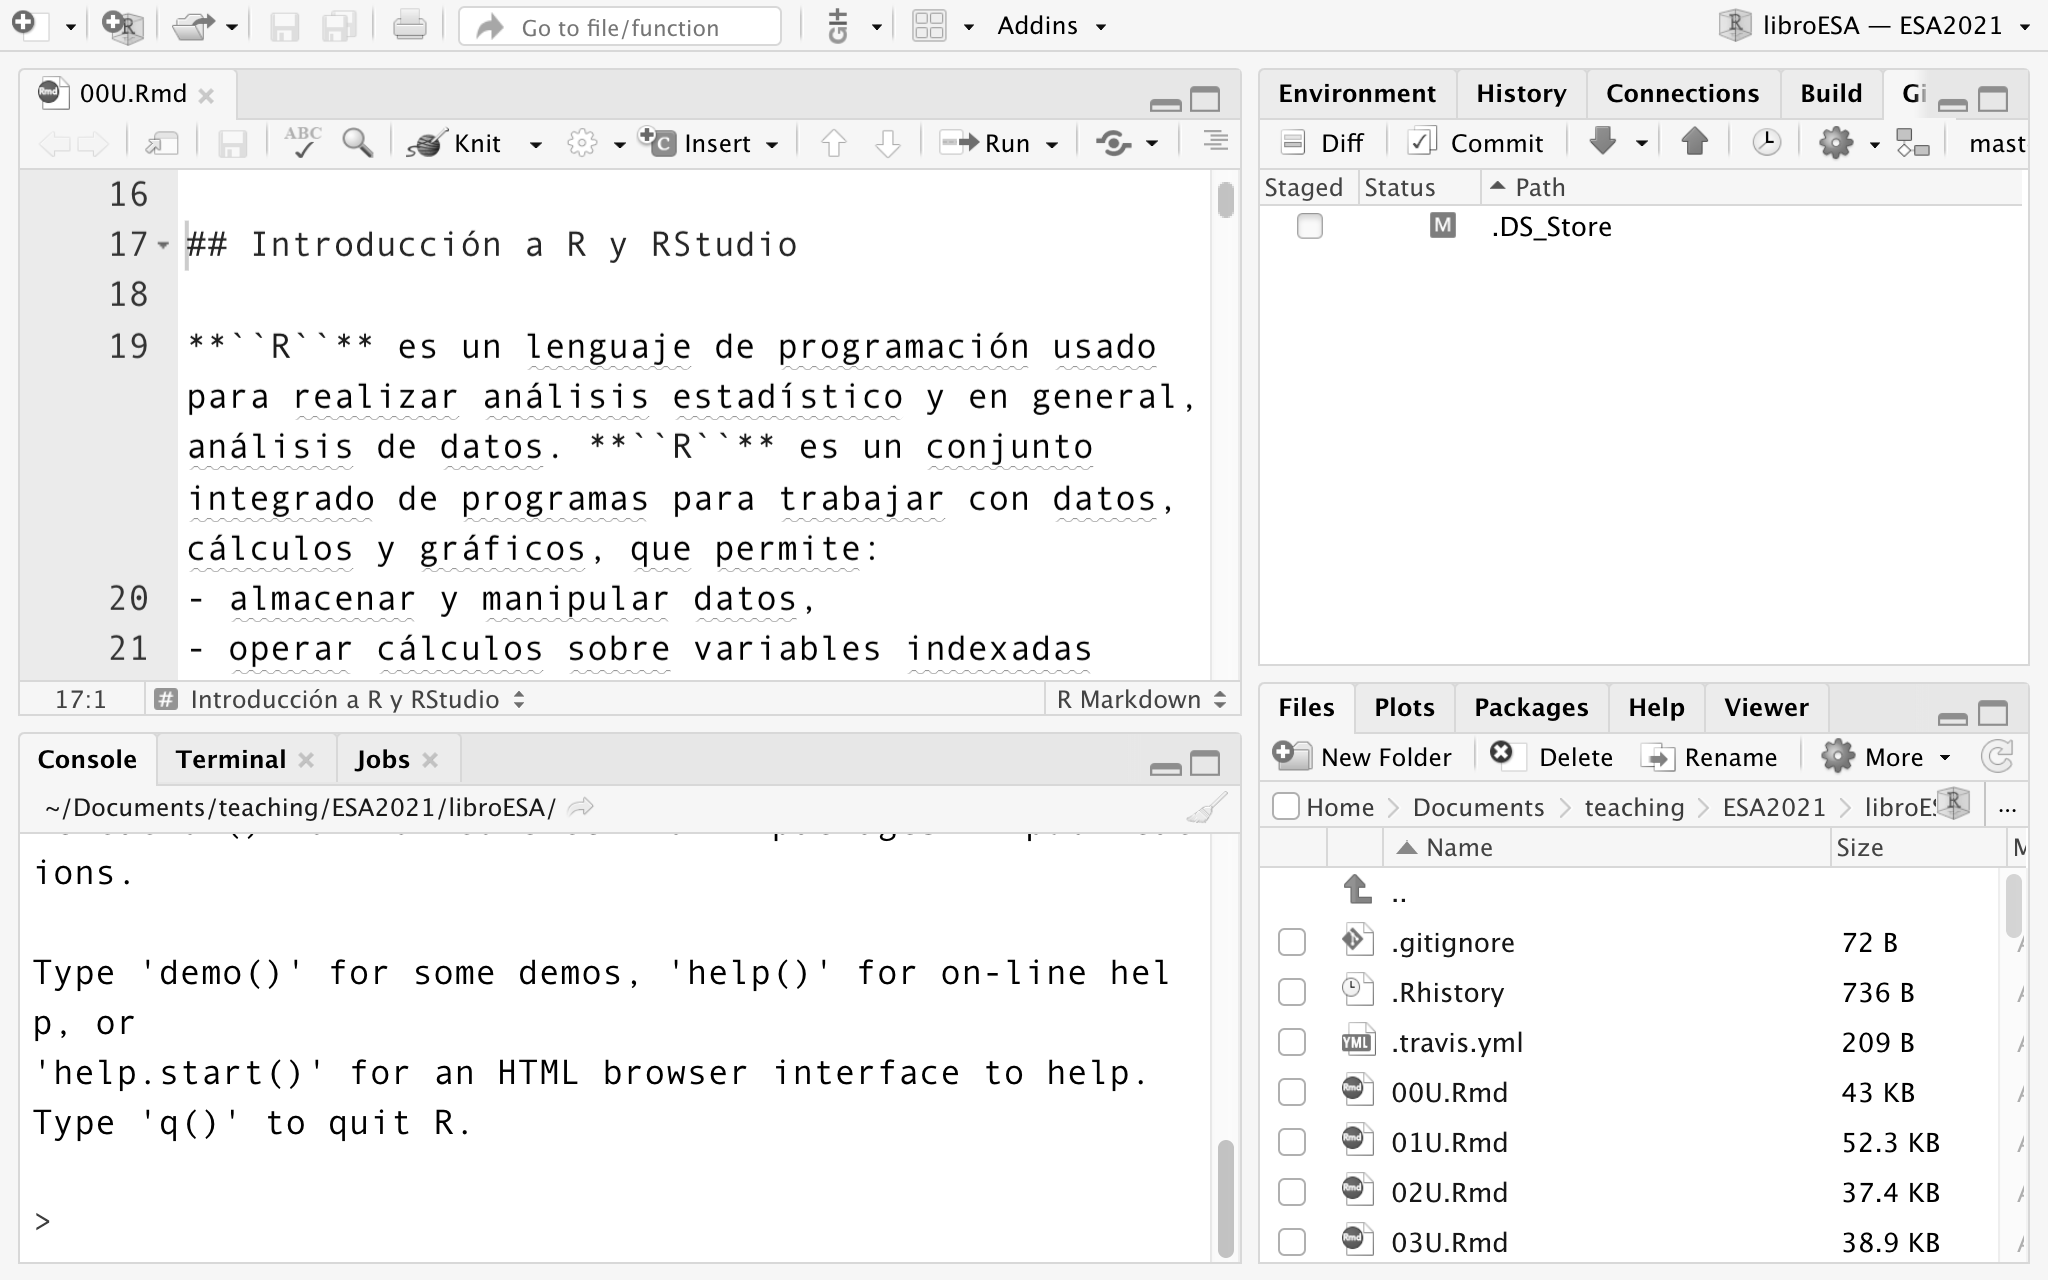
\includegraphics[width=0.8\linewidth]{imagenes/rstudio_entorno} 

}

\caption{RStudio Escritorio}\label{fig:unnamed-chunk-139}
\end{figure}

\begin{itemize}
\item
  Básicamente, la interfaz se compone de diferentes paneles. Sobre el lado izquierdo hay un panel grande y en el lado derecho hay dos paneles más pequeños. Al comenzar a trabajar en \texttt{RStudio}, habrá un cuarto panel que se activa al abrir un nuevo documento.
\item
  Al crear ese nuevo archivo hay cuatro paneles: dos a la izquierda y dos a la derecha. Es posible ajustar estos paneles moviendo la barra que los separa. También se puede deslizar el divisor del medio para ajustar el ancho de los paneles y en el lado derecho también es posible ajustar las alturas relativas de estos paneles.
\item
  En la esquina de cada panel hay un botón de minimizar, para ocultar cualquier panel. Se puede maximizar nuevamente haciendo \emph{clic} sobre el mismo o en el botón que muestra dos paneles.
\item
  Esta es la forma predeterminada para configurar \texttt{RStudio}. Cualquier documento que se cree se encontrará en el panel superior \textbf{izquierdo} mientras que en el inferior izquierdo está la consola de \textbf{\texttt{R}}, que es un área donde se pueden escribir comandos directamente. En el lado \textbf{derecho}, el panel superior es básicamente información sobre el entorno en el que está trabajando.
\item
  En la parte inferior derecha hay un panel que tiene varias pestañas. El primero permite ver la estructura de los archivos, por lo que es parecido a una ventana estándar que se usa para navegar en cualquier sistema operativo.
\end{itemize}

\begin{figure}

{\centering 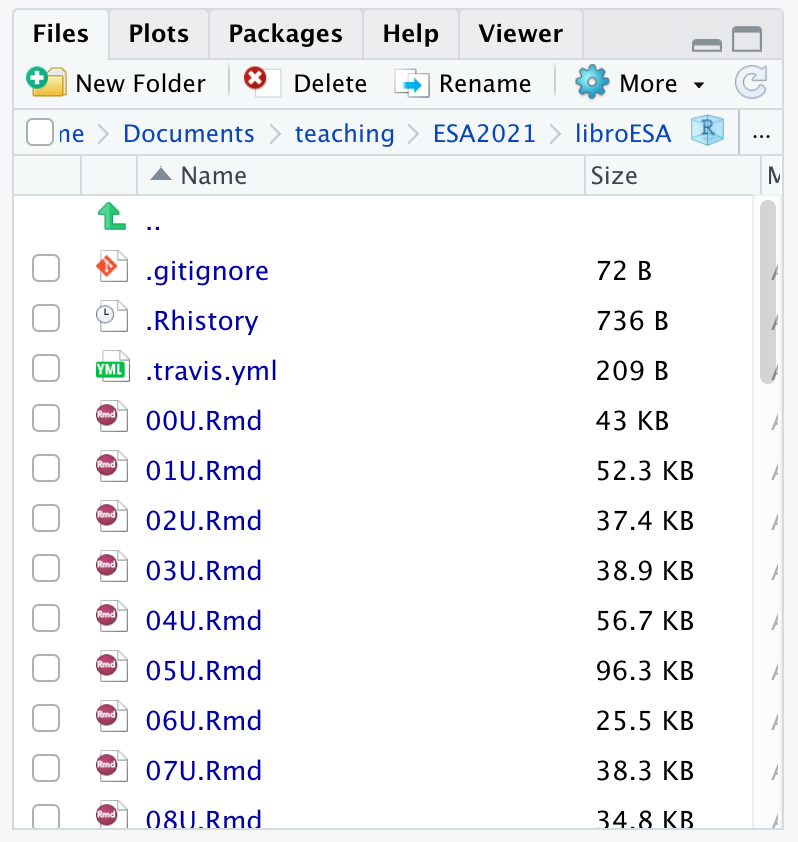
\includegraphics[width=0.6\linewidth]{imagenes/pan_der_inf} 

}

\caption{panel Derecho Inferior de RStudio}\label{fig:unnamed-chunk-140}
\end{figure}

\begin{itemize}
\tightlist
\item
  Hay una pestaña que enumera los paquetes que se han instalado.
\end{itemize}

\begin{figure}

{\centering 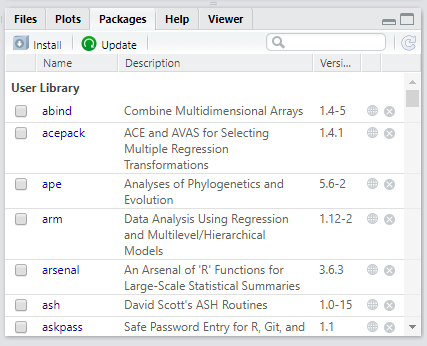
\includegraphics[width=0.6\linewidth]{imagenes/paquetes} 

}

\caption{Paquetes de RStudio}\label{fig:unnamed-chunk-141}
\end{figure}

\begin{itemize}
\tightlist
\item
  La otra es una pestaña de ayuda, ya que en \textbf{\texttt{R}}, si uno desea ayuda sobre cualquier cosa, se la puede obtener escribiendo un signo de interrogación y luego el nombre del objeto sobre el que desea ayuda:
\end{itemize}

\begin{Shaded}
\begin{Highlighting}[]
\StringTok{\textasciigrave{}}\AttributeTok{?}\StringTok{\textasciigrave{}}\NormalTok{(mean)}
\end{Highlighting}
\end{Shaded}

\begin{itemize}
\tightlist
\item
  Se puede ver que, al ejecutar ese comando, se obtiene un archivo de ayuda sobre la media. También es posible obtener uno sobre la mediana, y así sucesivamente.
\end{itemize}

\begin{Shaded}
\begin{Highlighting}[]
\StringTok{\textasciigrave{}}\AttributeTok{?}\StringTok{\textasciigrave{}}\NormalTok{(median)}
\end{Highlighting}
\end{Shaded}

Se obtendrá:

\begin{figure}

{\centering 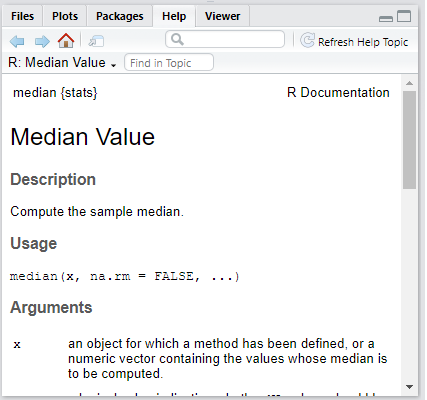
\includegraphics[width=0.6\linewidth]{imagenes/ayuda} 

}

\caption{R}\label{fig:unnamed-chunk-144}
\end{figure}

\begin{itemize}
\tightlist
\item
  Entonces, si hace falta ayuda, aparecerá en dicha pestaña. Hay que tener en cuenta que es posible modificar la configuración de estos paneles. Los pasos para hacerlo son:
\end{itemize}

\begin{quote}
Menú \textgreater{} Herramientas
\end{quote}

\begin{itemize}
\item
  Dentro de herramientas (\emph{Tools}) se encuentran las `Opciones globales' (\emph{Global Options}). Este menú ofrece todo tipo de posibilidades para configurar \texttt{RStudio} y el entorno. Para cambiar la ubicación de la consola y el entorno, hay que clicar arriba, donde dice `Entorno', sobre el cuadro desplegable y aplicarlo. Al volver, se verá en el lado izquierdo, el documento en el que se está trabajando y debajo, el panel de `Entorno'.
\item
  También es posible cambiar el color del esquema, dentro de las `Opciones globales' puedes ver algunas opciones de apariencia. El tema predeterminado tiene blanco de fondo con un texto en negro. Pero no es el único, sino que existen diferentes temas que se pueden aplicar.
\end{itemize}

\hypertarget{workflow}{%
\subsection{Workflow}\label{workflow}}

Esta sección trata sobre el flujo de trabajo (\emph{workflow}) en \texttt{RStudio}. Existen muchas cosas sobre el trabajo en \texttt{R} que los encuentran confusas. Sin embargo, hay formas en las que se pueden simplificar problemas: sistematizando una buena práctica del flujo de trabajo desde el principio.

\hypertarget{proyectos-r-studio}{%
\subsubsection{Proyectos R Studio}\label{proyectos-r-studio}}

Una de las cuestiones más comunes que generan dificultades en \textbf{\texttt{R}}, es que no provee las facilidades de un software estadístico estándar con el cual apuntar y hacer \emph{clic} dentro de la misma interfaz. Específicamente se dificulta el acceso a los archivos y el guardado utilizando rutas de archivo, en especial cuando esas rutas (\texttt{paths}) son extensas.

La forma más sencilla de minimizar esta dificultad es trabajar con lo que se llama un documento de tipo \textbf{Proyecto de RStudio}. Este es el primer paso a seguir: usar los archivos de proyecto de \texttt{RStudio}. Antes que nada, ¿Qué es un archivo de proyecto de \texttt{RStudio}?

\begin{itemize}
\tightlist
\item
  Es un archivo creado por \texttt{RStudio} que tiene una extensión de \texttt{.Rproj}, y esencialmente lo que hace es almacenar información sobre la carpeta que lo contiene. Así que para guardar este archivo de proyecto dentro de una carpeta en particular, hay que tener en cuenta que dentro del proyecto se guardará información sobre la carpeta que se encuentra en su sistema de archivos, y también guardará información sobre el estado anterior del proyecto. Cuando se genera un archivo de proyecto, primero se abrirá en \texttt{RStudio} y de este modo se podrá acceder a la información sobre la carpeta en la que se encuentra almacenado este proyecto.
\end{itemize}

\hypertarget{organizaciuxf3n}{%
\subsubsection{Organización}\label{organizaciuxf3n}}

Una de los aspectos clave es que, al trabajar con archivos de proyecto, es necesario organizarse. Una forma sencilla de trabajar con \texttt{RStudio} es tener un proceso pre-establecido por el que pasar cada vez que se inicie un nuevo proyecto. El proceso que se sugiere en este libro consiste en:

\begin{enumerate}
\def\labelenumi{\arabic{enumi}.}
\item
  Crear un nuevo proyecto de \texttt{RStudio}, por el cual se generará una carpeta dentro del directorio local.
\item
  Luego, dentro de esa carpeta crear una sub-carpeta llamada `datos'. Ahí es donde se guardarán todos los archivos de datos relacionados con el proyecto.
\item
  También, crear una carpeta llamada \texttt{r\_docs} que es donde se guardan todos los documentos de \textbf{\texttt{R}} y de \texttt{RStudio}.
\item
  En caso que haya imágenes o medios asociados con el proyecto, se aconseja generar una carpeta llamada `imágenes'.
\end{enumerate}

En resumen, siguiendo el tipo de organización aquí propuesta, hay un directorio donde se guardan todos los proyectos de \texttt{R\ Studio}. Tal como se aclaró antes: la información del proyecto se almacena dentro de una carpeta, donde a su vez hay tres carpetas más: una donde se encuentran los archivos de \texttt{datos}, otra donde guardar todos los \texttt{documentos} de \textbf{\texttt{R}} y \texttt{RStudio}, y una última carpeta para las \texttt{imágenes}. Además, dentro de esa carpeta grande habrá un archivo de \texttt{RStudio\ Project}, con el nombre que el usuario le haya asignado.

\hypertarget{utilidad}{%
\subsubsection{Utilidad}\label{utilidad}}

¿Por qué este procedimiento de organización del flujo de trabajo es útil? Porque respetando la estructura de las carpetas, es posible encontrar los archivos de manera sencilla, optimizando tiempo y espacio. Esta estructura se puede ver en la ruta del archivo, que será similar a /Usuarios/Nombreusuario/Documentos/RProjects\ldots etc. Esta es una ruta a un archivo de datos que se almacena en el disco duro, en la unidad correspondiente, que puede ser \texttt{C} o \texttt{U}, por ejemplo.

\textbf{Desventaja 1}

Dentro de una carpeta llamada \texttt{Usuarios}, ingresando a una carpeta denominada ``tunombre'' (aquí cada uno puede colocar su propio nombre de usuario), dentro de la carpeta llamada ``Documentos'' y luego, dentro de otra carpeta, se encuentra el nuevo proyecto creado. En esta última, finalmente, está la subcarpeta de ``datos''. Por lo tanto, cada vez que se desee acceder a ese archivo de datos, tanto para cargarlo como guardarlo, se debe llamar a esa gran cadena de texto, que es la ruta al archivo, lo cual puede resultar complicado.

\textbf{Desventaja 2}

Si se cambia de computadora donde fue creado un archivo de \textbf{\texttt{R}} a otra que no tenga el sistema de archivos que se ha descrito en este libro, entonces se debe reescribir todo el código de \textbf{\texttt{R}} para poder acceder al archivo deseado. Esto se debe a que podría estar guardado en una ubicación diferente a la de mi archivo local. Al usar un proyecto de \texttt{RStudio} se puede utilizar lo que se conoce como ``rutas relativas''. También, hay un camino mucho más corto que implica colocar dos puntos y una barra al inicio de la ruta. Los puntos representan la carpeta del proyecto que se encuentra en una ubicación diferente a la del archivo que se está editando. Dondequiera que esa carpeta esté almacenada, no es necesario saberlo porque el proyecto de \texttt{RStudio} se redirige automáticamente allí cuando se implementan los puntos. Todo lo que hay que hacer es poner los puntos seguidos de una barra, luego el nombre de la carpeta de datos y de nuevo barra, seguido el nombre del archivo al que se intenta acceder. Por ejemplo, \texttt{../nombrecarpeta/nombrearchivo.Rmd}

De seguido, se presenta un segundo ejemplo utilizando la estructura de carpetas propuesta. Si se almacenan los archivos de \texttt{RStudio} dentro de una carpeta llamada ``docs\_r'', es necesario salir de la misma y luego volver a ``mis\_datos''. Eso es lo que los puntos dobles hacen: subir de nivel. En concreto, las acciones que lleva a cabo son salir de `docs\_r' e ir a la carpeta de datos. Sin embargo, cuando hay muchos archivos, esto puede resultar un poco engorroso.

\hypertarget{crear-un-proyecto-de-rstudio}{%
\subsubsection{Crear un Proyecto de RStudio}\label{crear-un-proyecto-de-rstudio}}

\begin{itemize}
\item
  Lo primero es seleccionar un directorio en alguna carpeta local del ordenador.
\item
  Luego abrir \texttt{RStudio} e ir al menú ``Archivo'', hacer clic en ``Nuevo Proyecto'' y así se obtendrá un cuadro de diálogo. Se puede crear un nuevo directorio con el proyecto o si ya existe un directorio que se pueda convertir en un proyecto de \texttt{RStudio}, también se puede seleccionar un directorio existente.
\item
  En siguiente paso es seleccionar en la opción superior para generar un proyecto, y luego crear el proyecto nuevo como un subdirectorio.
\item
  Lo siguiente es buscar dónde guardar este proyecto. Si se desea mantener todos los proyectos juntos es necesario crear una carpeta llamada, por ejemplo, ``proyectosr'' donde colocar todos los proyectos de \textbf{\texttt{R}}. Como nombre del directorio se solicita el nombre del archivo de proyecto de \texttt{RStudio}, en este caso puede llamarse ``primer\_proyecto''.
\item
  Como resultado, a pesar de que nada parece cambiar, en la pestaña de archivos (margen inferior), se notifica que uno se encuentra en la carpeta o directorio seleccionados. En este caso, dentro de la carpeta de todos los proyectos de \textbf{\texttt{R}} y, a su vez, en la carpeta llamada ``primer\_proyecto'' que es como se ha nombrado a este proyecto. Se puede navegar dentro del proyecto desde aquí.
\end{itemize}

\textbf{Recordatorio}

\begin{itemize}
\tightlist
\item
  \textbf{\texttt{R}} distingue entre mayúsculas y minúsculas, por lo que siempre es recomendable escribir todo en minúsculas.
\end{itemize}

\hypertarget{crear-un-archivo-de-r}{%
\subsubsection{Crear un archivo de R}\label{crear-un-archivo-de-r}}

Lo siguiente es crear un documento en el que se quiere trabajar. En este libro se usa el ejemplo de un archivo de \texttt{RMarkdown}, aunque existen otros tipos de archivos de \textbf{\texttt{R}}. Uno de los más utilizados es el \texttt{R\ script}, equivalente a una sintaxis de \textbf{SPSS} o \emph{do-file} de \textbf{STATA}.

\begin{itemize}
\item
  Crear un nuevo archivo de tipo \texttt{R\ Markdown}. Al seleccionar sobre el botón de crear archivo (margen superior izquierdo, identificado con el signo ``+'' en color verde), aparecerá una ventana. Allí, se coloca el título al documento, que se puede llamar ``primer\_documento'', y también el nombre del autor. No es necesario poner el nombre del autor, se puede dejar ese espacio en blanco. Y por último, se selecciona el ``Formato de salida'', que crea el archivo de \texttt{R\ Markdown}.
\item
  Es posible ver que en el nuevo documento de \texttt{R\ Markdown} ya hay texto, que es un ejemplo de documento, el cual se puede borrar en su totalidad y cargar la información que se desee. En un documento de \texttt{R\ Markdown}, las áreas grises son lo que se conoce como ``fragmentos de código'' o \emph{chunks}. Allí es donde se dan instrucciones a \textbf{\texttt{R}}, como comandos o fórmulas, sobre las que trabaja el programa.
\item
  Fuera, en el área blanca, se puede escribir texto. Se presenta un ejemplo simple, en el que se inserta un fragmento de código de varias maneras.
\end{itemize}

También hay atajos de teclado que puedes usar:

\begin{Shaded}
\begin{Highlighting}[]
\SpecialCharTok{*}\NormalTok{ Insert code chunk }\ControlFlowTok{in}\NormalTok{ PC}\SpecialCharTok{:}\NormalTok{ Ctrl}\SpecialCharTok{+}\NormalTok{Alt}\SpecialCharTok{+}\NormalTok{I}
\SpecialCharTok{*}\NormalTok{ Insert code chunk }\ControlFlowTok{in}\NormalTok{ Max}\SpecialCharTok{/}\NormalTok{Linux}\SpecialCharTok{:}\NormalTok{ Cmd}\SpecialCharTok{+}\NormalTok{Option}\SpecialCharTok{+}\NormalTok{I}
\end{Highlighting}
\end{Shaded}

\textbf{En resumen}, cuando haya un nuevo proyecto en el que se esté trabajando, se recomienda generar un nuevo archivo de proyecto en \texttt{RStudio}. Dentro de esa carpeta, generar otra carpeta donde almacenar los datos (que aquí se ha llamado ``r\_docs''), como los documentos de \texttt{R\ Markdown} o \texttt{R\ script}.

\hypertarget{rmarkdown}{%
\subsection{RMarkdown}\label{rmarkdown}}

La manera más sencilla de interactuar con \textbf{\texttt{R}} es a través de documentos conocidos como archivos de \textbf{R Markdown}, que ya se ha visto a modo de ejemplo en la sección anterior\footnote{Un resumen de las funciones y comandos que dispone R Markdown puede encontrarse \href{https://www.rstudio.com/wp-content/uploads/2015/02/rmarkdown-cheatsheet.pdf}{aquí}}. Estos documentos son una combinación de varios tipos de información. Por un lado, lo que se conoce como ``fragmentos de código'' (\emph{code chunks}), que son un tipo de ventanas en \textbf{\texttt{R}} donde se escribe código para ejecutar análisis. También, fuera de esos fragmentos de código se puede escribir texto. En esta sección se explicará con mayor detalle cómo formatear el texto en el documento de \textbf{\texttt{R}}. Para ello seguir los pasos:

\begin{itemize}
\item
  Abrir el primer proyecto de \texttt{RStudio}, el cual estará alojado en el directorio del equipo local llamado ``proyectos\_r'' o similar.
\item
  Dentro de esa carpeta, seleccionar el documento llamado ``primer\_proyecto.Rproj''.
\item
  Otras carpetas que se encuentran allí son: ``datos'' e ``imágenes''.
\item
  Descargar una foto de Internet o seleccionar una foto antigua que se encuentre en la computadora y
  guardarla en la carpeta de ``imágenes''.
\item
  Crear un nuevo documento clicando en la barra superior de RStudio llamada ``documentos'', y luego en \texttt{R\ Markdown}. Otra opción es clicar sobre el ícono de una hoja blanca con un círculo verde en la esquina superior izquierda de la barra de herramientas de \texttt{RStudio}. Aparecerá una ventana, que se rellena con el título y el autor. Luego, guardarlo con un nombre al archivo y almacenarlo en la carpeta del proyecto, en ``documentos\_r''.
\item
  El documento posee un \emph{template}, clicar sobre el botón ``Knit'', acompañado de un ícono de un ovillo de lana y unas agujas de tejer (barra superior izquierda). Se obtendrá un archivo de tipo \texttt{HTML} con el título, la fecha y el autor, que se puede eliminar en caso de ser necesario.
\end{itemize}

\hypertarget{agregar-texto}{%
\subsubsection{Agregar texto}\label{agregar-texto}}

La cantidad de símbolos de numeral (\#) indica el nivel del título o subtítulo que se desea editar. Es necesario dejar un espacio entre el numeral y el texto que se escribe para obtener los títulos en negrita y sin el símbolo. Se debe utilizar el primer nivel de títulos en cada documento \texttt{R\ Markdown}. Se prueban los niveles diferentes en un documento de \texttt{R\ Markdown} de la siguiente manera:

\begin{Shaded}
\begin{Highlighting}[]
\CommentTok{\# Título nivel 1 Título nivel 2 Título nivel 3 Título nivel 4}
\end{Highlighting}
\end{Shaded}

\textbf{Recordatorio: } Clicar Control + S constantemente para guardar los cambios efectuados en el documento, a medida que se trabaja sobre él.

\hypertarget{listas}{%
\subsubsection{Listas}\label{listas}}

\begin{itemize}
\item
  Se utiliza el símbolo del asterisco para realizar bullet-points (* Bullet)
\item
  Para un sub-bullet se usa el signo sumatorio (+ Sub-bullet)
\item
  Para un tercer nivel de sub-bullet, el signo de restas (- Tercer nivel de bullets)
\item
  Es importante, además de los símbolos, indentar las líneas cada vez que reduzca mi número de bullets
  en una lista. Espaciar entre el símbolo y el contenido de la lista. Además hay que dejar un espacio una vez finalizada la lista y antes de comenzar otra nueva.
\item
  Se puede hacer una prueba creando una lista sobre ``Materias que no me gustan de mi carrera''. Para presentar la lista, se debe agregar una línea de texto común, con su descripción.
\item
  Luego, clicar en ``Knit'' para generar el documento.
\end{itemize}

\hypertarget{editar-texto}{%
\subsubsection{Editar texto}\label{editar-texto}}

\begin{itemize}
\tightlist
\item
  Para incluir algún formato de texto, se deben utilizar los siguientes símbolos al inicio y al final de cada palabra o grupo de palabras que se desea editar:
\end{itemize}

\begin{Shaded}
\begin{Highlighting}[]
\SpecialCharTok{*}\NormalTok{Itálicas}\SpecialCharTok{*}
    
\ErrorTok{**}\NormalTok{Resaltado}\SpecialCharTok{**}
    
\NormalTok{Texto }\SpecialCharTok{\^{}}\NormalTok{superscript}\SpecialCharTok{\^{}}
    
\NormalTok{Texto }\SpecialCharTok{\textasciitilde{}}\NormalTok{subscript}\SpecialCharTok{\textasciitilde{}}
\end{Highlighting}
\end{Shaded}

\hypertarget{insertar-imuxe1genes}{%
\subsubsection{Insertar imágenes}\label{insertar-imuxe1genes}}

\begin{itemize}
\tightlist
\item
  Las imágenes son fáciles de agregar, siguiendo las líneas de código siguiente:
\end{itemize}

\begin{Shaded}
\begin{Highlighting}[]
\SpecialCharTok{!}\NormalTok{[Caption }\ControlFlowTok{for}\NormalTok{ image](filepath\_for\_image)}
\end{Highlighting}
\end{Shaded}

\begin{itemize}
\item
  Se puede hacer una prueba agregando una foto que nos guste.
\item
  Se puede colocar el epígrafe de la foto del siguiente modo:
\end{itemize}

\begin{Shaded}
\begin{Highlighting}[]
\SpecialCharTok{!}\NormalTok{[Figura }\DecValTok{1}\SpecialCharTok{:}\NormalTok{ Mi mascota hermosa}\SpecialCharTok{:}\NormalTok{ Nina](imagenes}\SpecialCharTok{/}\NormalTok{nina.jpeg)}
\end{Highlighting}
\end{Shaded}

\begin{figure}
\centering
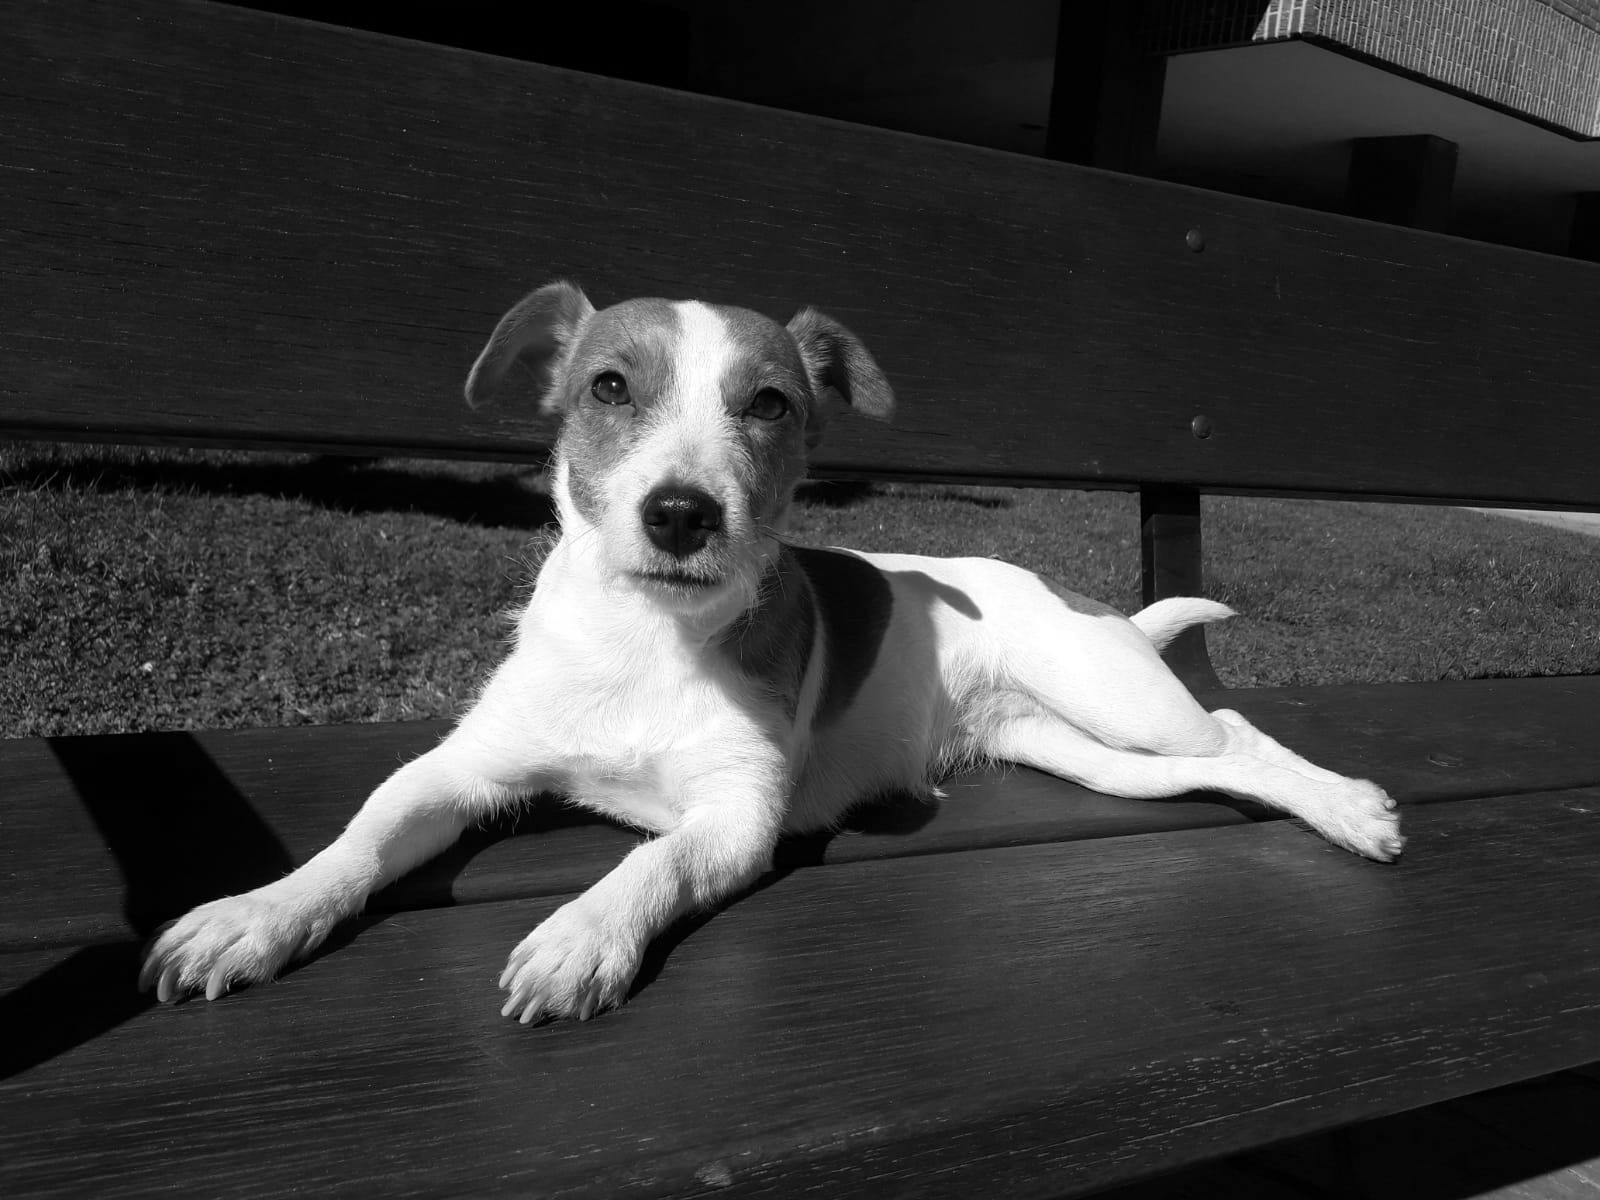
\includegraphics{imagenes/nina.jpeg}
\caption{Figura 1: Mi mascota: Nina}
\end{figure}

\begin{itemize}
\tightlist
\item
  También es posible seleccionar el tamaño de la imagen.
\end{itemize}

\begin{Shaded}
\begin{Highlighting}[]
\SpecialCharTok{!}\NormalTok{[Nina](imagenes}\SpecialCharTok{/}\NormalTok{nina.jpeg)\{width}\OtherTok{=}\DecValTok{50}\NormalTok{\%\}}
\end{Highlighting}
\end{Shaded}

\begin{figure}
\centering
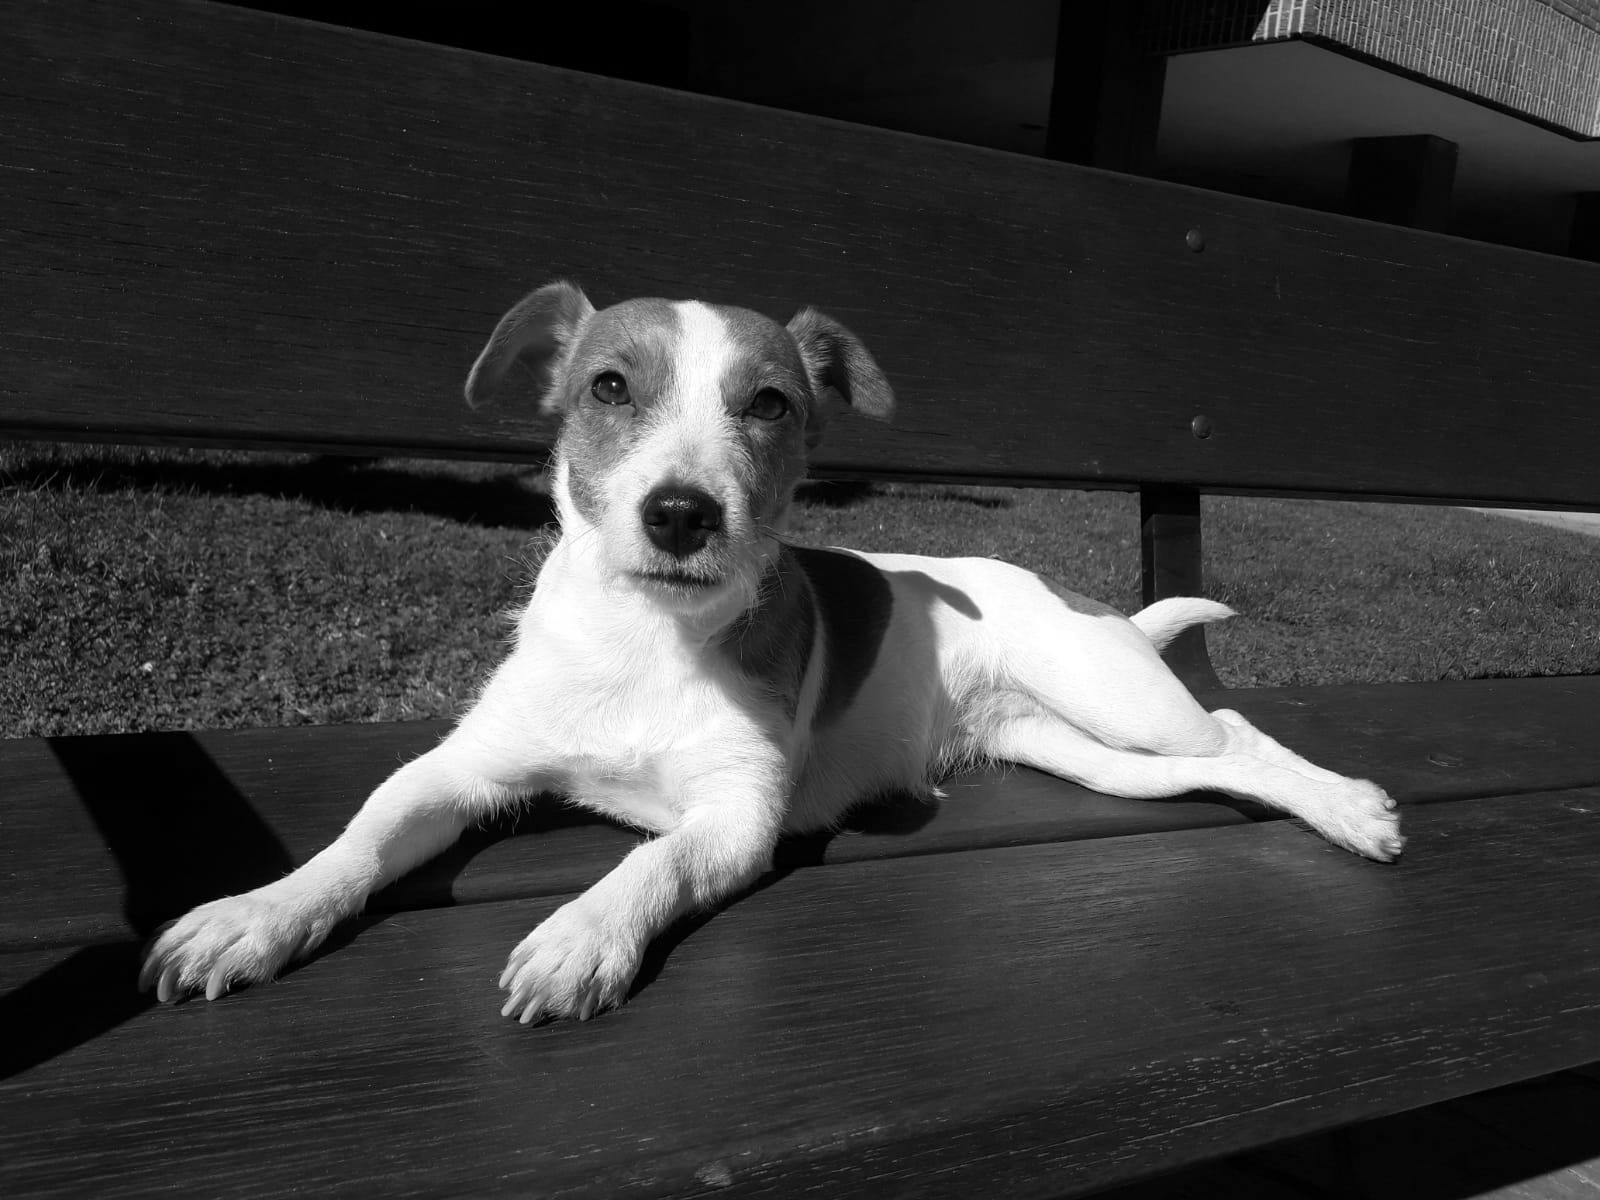
\includegraphics[width=0.5\textwidth,height=\textheight]{imagenes/nina.jpeg}
\caption{Nina}
\end{figure}

\hypertarget{enlaces}{%
\subsubsection{Enlaces}\label{enlaces}}

\begin{itemize}
\tightlist
\item
  Para incluir un enlace se debe:
\end{itemize}

\begin{Shaded}
\begin{Highlighting}[]
\NormalTok{Incluir entre corchetes [lo que aparecerá] en el texto y, seguido, entre paréntesis (el enlace que redirige al sitio que se seleccione).}
\end{Highlighting}
\end{Shaded}

\href{www.google.com.ar}{Link a google}

\hypertarget{tips-para-escribir-cuxf3digo-en-r}{%
\subsubsection{Tips para escribir código en R}\label{tips-para-escribir-cuxf3digo-en-r}}

\begin{itemize}
\tightlist
\item
  A la hora de escribir en este lenguaje de programación, hay que conocer algunas funcionalidades que permiten resolver acciones claves y responder a dudas de manera simple. Para obtener información sobre una función concreta, se puede utilizar alguna de las siguientes funciones:
\end{itemize}

\begin{Shaded}
\begin{Highlighting}[]
\FunctionTok{help}\NormalTok{(solve)}
\end{Highlighting}
\end{Shaded}

\begin{Shaded}
\begin{Highlighting}[]
\StringTok{\textasciigrave{}}\AttributeTok{?}\StringTok{\textasciigrave{}}\NormalTok{(solve)}
\end{Highlighting}
\end{Shaded}

\begin{itemize}
\item
  Las mayúsculas y minúsculas importan. \textbf{\texttt{R}} es un lenguaje de expresiones que es sensible a las mismas y responde de manera diferente a cada una.
\item
  Las órdenes elementales consisten en expresiones o en asignaciones. Las órdenes se separan con un punto y coma, (`;'), o cambiando de línea.
\item
  Las flechas verticales permiten recuperar órdenes previas y ejecutarlas y las horizontales permiten desplazarnos dentro de una orden para corregirla.
\item
  Para eliminar objetos puede utilizar la orden ``rm'', por ejemplo:
\end{itemize}

\begin{Shaded}
\begin{Highlighting}[]
\FunctionTok{rm}\NormalTok{(x, y, z, cabello, perro, bonito)}
\end{Highlighting}
\end{Shaded}

\hypertarget{primerospasos}{%
\subsection{Primeros pasos en R}\label{primerospasos}}

\hypertarget{funciones-y-comandos-elementales}{%
\subsubsection{Funciones y comandos elementales}\label{funciones-y-comandos-elementales}}

Las entidades que crea \textbf{\texttt{R}} durante una sesión de trabajo se denominan \emph{objetos}. Estos pueden ser números, cadenas, vectores, matrices, funciones o estructuras más generales construidas a partir de estos elementos. Estos objetos se guardan por nombre y se almacenan en un área dedicada llamada ``espacio de trabajo'' o \emph{environment}. En cualquier momento, es posible verificar los objetos disponibles en el espacio de trabajo usando el comando:

\begin{Shaded}
\begin{Highlighting}[]
\FunctionTok{ls}\NormalTok{()}
\end{Highlighting}
\end{Shaded}

Para eliminar un objeto del espacio de trabajo, se usa la función \texttt{rm()}. La función espera el nombre del objeto que se desea eliminar como argumento. Suponiendo que hay un objeto llamado ``cosa'', puede eliminarse con el comando:

\begin{Shaded}
\begin{Highlighting}[]
\FunctionTok{rm}\NormalTok{(cosa)}
\end{Highlighting}
\end{Shaded}

Al iniciar una nueva sesión de trabajo, se recomienda retirar los objetos existentes en el área de trabajo. Un comando útil para este propósito es:

\begin{Shaded}
\begin{Highlighting}[]
\FunctionTok{rm}\NormalTok{(}\AttributeTok{list =} \FunctionTok{ls}\NormalTok{())}
\end{Highlighting}
\end{Shaded}

Se puede almacenar el espacio de trabajo con la función:

\begin{Shaded}
\begin{Highlighting}[]
\FunctionTok{save.image}\NormalTok{()}
\end{Highlighting}
\end{Shaded}

Esto guarda todos los objetos contenidos en el espacio de trabajo en un archivo binario ``.Rdata''. La opción predeterminada se puede cambiar especificando en la llamada a \texttt{save.image()} el nombre, por ejemplo, ``myfile.Rdata'', que desea darle al archivo.

\begin{Shaded}
\begin{Highlighting}[]
\FunctionTok{save.image}\NormalTok{(}\AttributeTok{archive =} \StringTok{"myfile.Rdata"}\NormalTok{)}
\end{Highlighting}
\end{Shaded}

El espacio de trabajo original se puede restaurar con la ayuda de la función:

\begin{Shaded}
\begin{Highlighting}[]
\FunctionTok{load}\NormalTok{(}\StringTok{".RData"}\NormalTok{)}
\end{Highlighting}
\end{Shaded}

o, si se ha optado por un nombre diferente al predeterminado:

\begin{Shaded}
\begin{Highlighting}[]
\FunctionTok{load}\NormalTok{(}\StringTok{"ilmiofile.Rdata"}\NormalTok{)}
\end{Highlighting}
\end{Shaded}

Las funciones:

\begin{Shaded}
\begin{Highlighting}[]
\FunctionTok{savehistory}\NormalTok{()}
\end{Highlighting}
\end{Shaded}

\begin{Shaded}
\begin{Highlighting}[]
\FunctionTok{loadhistory}\NormalTok{()}
\end{Highlighting}
\end{Shaded}

permiten guardar en formato \texttt{ASCII} y recargar en \textbf{\texttt{R}} el historial de los comandos enviados. El argumento de archivo que permite especificar un nombre que no sea la elección predeterminada, es ``.Rhistory''.

Finalmente, la función \texttt{setwd()} permite cambiar la carpeta de trabajo. Es una buena idea dedicar una carpeta separada a cada proyecto en el que esté trabajando para evitar la superposición de datos. El directorio de trabajo actual se puede ver con el comando \texttt{getwd()}.

Los comandos básicos constan de expresiones o asignaciones. Si el comando es una expresión, \textbf{\texttt{R}} devuelve el resultado de la evaluación, como se muestra en los siguientes ejemplos:

\begin{Shaded}
\begin{Highlighting}[]
\DecValTok{12} \SpecialCharTok{\textgreater{}} \DecValTok{10}
\end{Highlighting}
\end{Shaded}

\begin{verbatim}
[1] TRUE
\end{verbatim}

\begin{Shaded}
\begin{Highlighting}[]
\DecValTok{1} \SpecialCharTok{+} \DecValTok{2} \SpecialCharTok{+} \DecValTok{3}
\end{Highlighting}
\end{Shaded}

\begin{verbatim}
[1] 6
\end{verbatim}

\begin{Shaded}
\begin{Highlighting}[]
\DecValTok{2} \SpecialCharTok{+} \DecValTok{3} \SpecialCharTok{*} \DecValTok{4}
\end{Highlighting}
\end{Shaded}

\begin{verbatim}
[1] 14
\end{verbatim}

\begin{Shaded}
\begin{Highlighting}[]
\DecValTok{3}\SpecialCharTok{/}\DecValTok{2} \SpecialCharTok{+} \DecValTok{1}
\end{Highlighting}
\end{Shaded}

\begin{verbatim}
[1] 2.5
\end{verbatim}

\begin{Shaded}
\begin{Highlighting}[]
\DecValTok{2} \SpecialCharTok{+}\NormalTok{ (}\DecValTok{3} \SpecialCharTok{*} \DecValTok{4}\NormalTok{)}
\end{Highlighting}
\end{Shaded}

\begin{verbatim}
[1] 14
\end{verbatim}

\begin{Shaded}
\begin{Highlighting}[]
\NormalTok{(}\DecValTok{2} \SpecialCharTok{+} \DecValTok{3}\NormalTok{) }\SpecialCharTok{*} \DecValTok{4}
\end{Highlighting}
\end{Shaded}

\begin{verbatim}
[1] 20
\end{verbatim}

\begin{Shaded}
\begin{Highlighting}[]
\DecValTok{4} \SpecialCharTok{*} \DecValTok{3}\SpecialCharTok{\^{}}\DecValTok{3}
\end{Highlighting}
\end{Shaded}

\begin{verbatim}
[1] 108
\end{verbatim}

Todas las funciones matemáticas que normalmente se encuentran en una calculadora de bolsillo están disponibles en \textbf{\texttt{R}} en forma de funciones básicas, que se recuerdan en la siguiente tabla:

\begin{itemize}
\item
  \texttt{sqrt} ---\textgreater{} raíz cuadrada
\item
  \texttt{abs} ---\textgreater{} valor absoluto
\item
  \texttt{sin,cos,tan} ---\textgreater{} funciones trigonométricas
\item
  \texttt{asin,acos,atan} ---\textgreater{} funciones trigonométricas inversas
\item
  \texttt{exp,log} ---\textgreater{} exponenciales y logaritmos naturales
\end{itemize}

\begin{Shaded}
\begin{Highlighting}[]
\FunctionTok{sqrt}\NormalTok{(}\DecValTok{2}\NormalTok{)}
\end{Highlighting}
\end{Shaded}

\begin{verbatim}
[1] 1.4
\end{verbatim}

\begin{Shaded}
\begin{Highlighting}[]
\FunctionTok{sin}\NormalTok{(}\FloatTok{3.14159}\NormalTok{)}
\end{Highlighting}
\end{Shaded}

\begin{verbatim}
[1] 0.0000027
\end{verbatim}

\begin{Shaded}
\begin{Highlighting}[]
\FunctionTok{sin}\NormalTok{(pi)}
\end{Highlighting}
\end{Shaded}

\begin{verbatim}
[1] 0.00000000000000012
\end{verbatim}

\begin{Shaded}
\begin{Highlighting}[]
\FunctionTok{sqrt}\NormalTok{(}\FunctionTok{sin}\NormalTok{(}\DecValTok{45} \SpecialCharTok{*}\NormalTok{ pi}\SpecialCharTok{/}\DecValTok{180}\NormalTok{))}
\end{Highlighting}
\end{Shaded}

\begin{verbatim}
[1] 0.84
\end{verbatim}

Una asignación evalúa una expresión guardando el resultado en un objeto con un nombre. La asignación se realiza mediante el símbolo \texttt{\textless{}-} o el símbolo \texttt{=}. También se puede asignar de izquierda a derecha con el símbolo \texttt{-\textgreater{}}. El resultado de una asignación no se muestra automáticamente. El usuario puede verlo recordando el nombre del objeto. Los objetos creados a través de una asignación se pueden reutilizar en expresiones y asignaciones posteriores, como se muestra en los siguientes ejemplos:

\begin{Shaded}
\begin{Highlighting}[]
\NormalTok{x }\OtherTok{\textless{}{-}} \FunctionTok{sqrt}\NormalTok{(}\DecValTok{2}\NormalTok{)}
\NormalTok{x}
\end{Highlighting}
\end{Shaded}

\begin{verbatim}
[1] 1.4
\end{verbatim}

\begin{Shaded}
\begin{Highlighting}[]
\NormalTok{x}\SpecialCharTok{\^{}}\DecValTok{3}
\end{Highlighting}
\end{Shaded}

\begin{verbatim}
[1] 2.8
\end{verbatim}

\begin{Shaded}
\begin{Highlighting}[]
\NormalTok{y }\OtherTok{\textless{}{-}}\NormalTok{ x}\SpecialCharTok{\^{}}\DecValTok{3}
\end{Highlighting}
\end{Shaded}

\begin{Shaded}
\begin{Highlighting}[]
\NormalTok{x }\OtherTok{\textless{}{-}} \DecValTok{10}
\NormalTok{x }\SpecialCharTok{\textgreater{}} \DecValTok{10}
\end{Highlighting}
\end{Shaded}

\begin{verbatim}
[1] FALSE
\end{verbatim}

\begin{Shaded}
\begin{Highlighting}[]
\NormalTok{x }\SpecialCharTok{\textless{}=} \DecValTok{10}
\end{Highlighting}
\end{Shaded}

\begin{verbatim}
[1] TRUE
\end{verbatim}

\begin{Shaded}
\begin{Highlighting}[]
\NormalTok{tf }\OtherTok{\textless{}{-}}\NormalTok{ x }\SpecialCharTok{\textgreater{}} \DecValTok{10}
\NormalTok{tf}
\end{Highlighting}
\end{Shaded}

\begin{verbatim}
[1] FALSE
\end{verbatim}

\hypertarget{valores-y-vectores}{%
\subsubsection{Valores y vectores}\label{valores-y-vectores}}

Para asignarle un valor a una variable, no es necesario utilizar espacios ni símbolos, excepto \texttt{\#} \texttt{.} o \texttt{\_} en el nombre de la variable:

\begin{Shaded}
\begin{Highlighting}[]
\NormalTok{mi\_valor }\OtherTok{\textless{}{-}} \DecValTok{30}  \CommentTok{\# número}
\NormalTok{un\_valor }\OtherTok{\textless{}{-}} \StringTok{"vaca"}  \CommentTok{\# caracteres}
\NormalTok{el\_valor }\OtherTok{\textless{}{-}} \ConstantTok{FALSE}  \CommentTok{\# booleano}
\end{Highlighting}
\end{Shaded}

Para crear un vector, se usa la función \texttt{c()}:

\begin{Shaded}
\begin{Highlighting}[]
\NormalTok{x }\OtherTok{\textless{}{-}} \FunctionTok{c}\NormalTok{(}\DecValTok{2}\NormalTok{, }\DecValTok{3}\NormalTok{, }\DecValTok{5}\NormalTok{, }\DecValTok{7}\NormalTok{, }\DecValTok{11}\NormalTok{)}
\NormalTok{x}
\end{Highlighting}
\end{Shaded}

\begin{verbatim}
[1]  2  3  5  7 11
\end{verbatim}

El vector puede contener texto o valores numéricos:

\begin{Shaded}
\begin{Highlighting}[]
\NormalTok{mi\_vector }\OtherTok{\textless{}{-}} \FunctionTok{c}\NormalTok{(}\DecValTok{6}\NormalTok{, }\DecValTok{12}\NormalTok{, }\DecValTok{80}\NormalTok{, }\DecValTok{120}\NormalTok{)}
\NormalTok{mi\_vector }\OtherTok{\textless{}{-}} \FunctionTok{c}\NormalTok{(}\StringTok{"María"}\NormalTok{, }\StringTok{"Esteban"}\NormalTok{, }\StringTok{"Juan"}\NormalTok{)}
\end{Highlighting}
\end{Shaded}

Si el vector contiene muchos elementos, puede ser más conveniente usar la función \texttt{scan()}, que permite ingresarlos uno por uno a través de la consola:

\begin{Shaded}
\begin{Highlighting}[]
\NormalTok{x }\OtherTok{\textless{}{-}} \FunctionTok{scan}\NormalTok{()}
\DecValTok{1}\SpecialCharTok{:}\DecValTok{1}
\DecValTok{2}\SpecialCharTok{:}\DecValTok{6}
\DecValTok{3}\SpecialCharTok{:}\DecValTok{3}
\DecValTok{4}\SpecialCharTok{:}\DecValTok{4}
\DecValTok{5}\SpecialCharTok{:}\DecValTok{2}
\end{Highlighting}
\end{Shaded}

Para crear una secuencia de números, puede usar el comando \texttt{a:b}:

\begin{Shaded}
\begin{Highlighting}[]
\NormalTok{xx }\OtherTok{\textless{}{-}} \DecValTok{1}\SpecialCharTok{:}\DecValTok{10}

\NormalTok{xx}
\end{Highlighting}
\end{Shaded}

\begin{verbatim}
 [1]  1  2  3  4  5  6  7  8  9 10
\end{verbatim}

\begin{Shaded}
\begin{Highlighting}[]
\NormalTok{xx }\OtherTok{\textless{}{-}} \DecValTok{100}\SpecialCharTok{:}\DecValTok{1}
\NormalTok{xx}
\end{Highlighting}
\end{Shaded}

\begin{verbatim}
  [1] 100  99  98  97  96  95  94  93  92  91  90  89  88  87  86  85  84  83
 [19]  82  81  80  79  78  77  76  75  74  73  72  71  70  69  68  67  66  65
 [37]  64  63  62  61  60  59  58  57  56  55  54  53  52  51  50  49  48  47
 [55]  46  45  44  43  42  41  40  39  38  37  36  35  34  33  32  31  30  29
 [73]  28  27  26  25  24  23  22  21  20  19  18  17  16  15  14  13  12  11
 [91]  10   9   8   7   6   5   4   3   2   1
\end{verbatim}

También se pueden crear vectores que contienen elementos repetidos:

\begin{Shaded}
\begin{Highlighting}[]
\FunctionTok{rep}\NormalTok{(}\DecValTok{2}\NormalTok{, }\AttributeTok{times =} \DecValTok{3}\NormalTok{)}
\end{Highlighting}
\end{Shaded}

\begin{verbatim}
[1] 2 2 2
\end{verbatim}

\begin{Shaded}
\begin{Highlighting}[]
\FunctionTok{rep}\NormalTok{(}\DecValTok{2}\NormalTok{, }\DecValTok{3}\NormalTok{)}
\end{Highlighting}
\end{Shaded}

\begin{verbatim}
[1] 2 2 2
\end{verbatim}

\begin{Shaded}
\begin{Highlighting}[]
\NormalTok{a }\OtherTok{\textless{}{-}} \FunctionTok{c}\NormalTok{(}\FunctionTok{rep}\NormalTok{(}\DecValTok{2}\NormalTok{, }\DecValTok{3}\NormalTok{), }\DecValTok{4}\NormalTok{, }\DecValTok{5}\NormalTok{, }\FunctionTok{rep}\NormalTok{(}\DecValTok{1}\NormalTok{, }\DecValTok{5}\NormalTok{))}
\NormalTok{a}
\end{Highlighting}
\end{Shaded}

\begin{verbatim}
 [1] 2 2 2 4 5 1 1 1 1 1
\end{verbatim}

Las operaciones aritméticas y lógicas básicas que se aplican a los escalares se pueden aplicar a los vectores:

\begin{Shaded}
\begin{Highlighting}[]
\NormalTok{x }\OtherTok{\textless{}{-}} \DecValTok{1}\SpecialCharTok{:}\DecValTok{10}
\NormalTok{x }\SpecialCharTok{*} \DecValTok{2}
\end{Highlighting}
\end{Shaded}

\begin{verbatim}
 [1]  2  4  6  8 10 12 14 16 18 20
\end{verbatim}

Los elementos de un vector se pueden extraer utilizando corchetes {[}{]} e indicando la posición del elemento a extraer entre corchetes:

\begin{Shaded}
\begin{Highlighting}[]
\NormalTok{xx[}\DecValTok{7}\NormalTok{]}
\end{Highlighting}
\end{Shaded}

\begin{verbatim}
[1] 94
\end{verbatim}

Incluso se pueden extraer más elementos al mismo tiempo:

\begin{Shaded}
\begin{Highlighting}[]
\NormalTok{xx[}\FunctionTok{c}\NormalTok{(}\DecValTok{2}\NormalTok{, }\DecValTok{3}\NormalTok{, }\DecValTok{5}\NormalTok{, }\DecValTok{7}\NormalTok{, }\DecValTok{11}\NormalTok{)]}
\end{Highlighting}
\end{Shaded}

\begin{verbatim}
[1] 99 98 96 94 90
\end{verbatim}

\begin{Shaded}
\begin{Highlighting}[]
\NormalTok{xx[}\DecValTok{85}\SpecialCharTok{:}\DecValTok{91}\NormalTok{]}
\end{Highlighting}
\end{Shaded}

\begin{verbatim}
[1] 16 15 14 13 12 11 10
\end{verbatim}

También se pueden guardar en nuevos vectores:

\begin{Shaded}
\begin{Highlighting}[]
\NormalTok{yy }\OtherTok{\textless{}{-}}\NormalTok{ xx[}\FunctionTok{c}\NormalTok{(}\DecValTok{1}\NormalTok{, }\DecValTok{2}\NormalTok{, }\DecValTok{4}\NormalTok{, }\DecValTok{8}\NormalTok{, }\DecValTok{16}\NormalTok{, }\DecValTok{32}\NormalTok{, }\DecValTok{64}\NormalTok{)]}
\NormalTok{yy}
\end{Highlighting}
\end{Shaded}

\begin{verbatim}
[1] 100  99  97  93  85  69  37
\end{verbatim}

Si los indicadores entre corchetes van precedidos de un signo negativo, los elementos correspondientes se eliminan del vector:

\begin{Shaded}
\begin{Highlighting}[]
\NormalTok{x }\OtherTok{\textless{}{-}} \FunctionTok{c}\NormalTok{(}\DecValTok{1}\NormalTok{, }\DecValTok{2}\NormalTok{, }\DecValTok{4}\NormalTok{, }\DecValTok{8}\NormalTok{, }\DecValTok{16}\NormalTok{, }\DecValTok{32}\NormalTok{)}
\NormalTok{x}
\end{Highlighting}
\end{Shaded}

\begin{verbatim}
[1]  1  2  4  8 16 32
\end{verbatim}

\begin{Shaded}
\begin{Highlighting}[]
\NormalTok{x[}\SpecialCharTok{{-}}\DecValTok{4}\NormalTok{]}
\end{Highlighting}
\end{Shaded}

\begin{verbatim}
[1]  1  2  4 16 32
\end{verbatim}

Al ingresar una variable a la consola, esta mostrará su contenido:

\begin{Shaded}
\begin{Highlighting}[]
\NormalTok{mi\_vector}
\end{Highlighting}
\end{Shaded}

\begin{verbatim}
[1] "María"   "Esteban" "Juan"   
\end{verbatim}

La función \texttt{length()} sirve para obtener el número de elementos en un vector o en una lista de objetos:

\begin{Shaded}
\begin{Highlighting}[]
\FunctionTok{length}\NormalTok{(mi\_vector)}
\end{Highlighting}
\end{Shaded}

\begin{verbatim}
[1] 3
\end{verbatim}

\hypertarget{matrices-y-listas}{%
\subsubsection{Matrices y listas}\label{matrices-y-listas}}

Una variable indexada (\emph{array}) es una colección de datos, por ejemplo numéricos, indexada por varios índices. \textbf{\texttt{R}} permite crear y manipular variables indexadas en general y en particular, matrices.

Las matrices se crean utilizando la función \texttt{matrix()}. En su forma más simple, el uso de la función implica especificar un vector que contiene los elementos de la matriz y el número de filas o columnas de la matriz.

\begin{Shaded}
\begin{Highlighting}[]
\NormalTok{x }\OtherTok{\textless{}{-}} \FunctionTok{matrix}\NormalTok{(}\FunctionTok{c}\NormalTok{(}\DecValTok{2}\NormalTok{, }\DecValTok{3}\NormalTok{, }\DecValTok{5}\NormalTok{, }\DecValTok{7}\NormalTok{, }\DecValTok{11}\NormalTok{, }\DecValTok{13}\NormalTok{), }\AttributeTok{nrow =} \DecValTok{3}\NormalTok{)}
\NormalTok{x}
\end{Highlighting}
\end{Shaded}

\begin{verbatim}
     [,1] [,2]
[1,]    2    7
[2,]    3   11
[3,]    5   13
\end{verbatim}

\begin{Shaded}
\begin{Highlighting}[]
\NormalTok{y }\OtherTok{\textless{}{-}} \FunctionTok{matrix}\NormalTok{(}\FunctionTok{c}\NormalTok{(}\DecValTok{2}\NormalTok{, }\DecValTok{3}\NormalTok{, }\DecValTok{5}\NormalTok{, }\DecValTok{7}\NormalTok{, }\DecValTok{11}\NormalTok{, }\DecValTok{13}\NormalTok{), }\AttributeTok{ncol =} \DecValTok{2}\NormalTok{)}
\NormalTok{y}
\end{Highlighting}
\end{Shaded}

\begin{verbatim}
     [,1] [,2]
[1,]    2    7
[2,]    3   11
[3,]    5   13
\end{verbatim}

Las \emph{array} pueden verse como matrices multidimensionales. Se crean usando la función \texttt{array()}. En su forma más simple, el uso de la función implica especificar un vector que contiene los elementos de la matriz y el número de elementos para cada dimensión usando el argumento \texttt{dim}.

\begin{Shaded}
\begin{Highlighting}[]
\NormalTok{w }\OtherTok{\textless{}{-}} \DecValTok{1}\SpecialCharTok{:}\DecValTok{20}
\NormalTok{ay }\OtherTok{\textless{}{-}} \FunctionTok{array}\NormalTok{(w, }\AttributeTok{dim =} \FunctionTok{c}\NormalTok{(}\DecValTok{5}\NormalTok{, }\DecValTok{2}\NormalTok{, }\DecValTok{2}\NormalTok{))}

\NormalTok{ay}
\end{Highlighting}
\end{Shaded}

\begin{verbatim}
, , 1

     [,1] [,2]
[1,]    1    6
[2,]    2    7
[3,]    3    8
[4,]    4    9
[5,]    5   10

, , 2

     [,1] [,2]
[1,]   11   16
[2,]   12   17
[3,]   13   18
[4,]   14   19
[5,]   15   20
\end{verbatim}

Hay que tener en cuenta que, de forma predeterminada, las matrices se forman insertando los distintos elementos por columna. Obviamente, la matriz se puede adquirir desde un archivo externo. Por ejemplo, suponiendo que el archivo \texttt{matdata} tiene el siguiente contenido:

\begin{Shaded}
\begin{Highlighting}[]
\DecValTok{1}\NormalTok{,}\DecValTok{24}\NormalTok{,}\DecValTok{32}\NormalTok{,}\DecValTok{36}\NormalTok{,}\DecValTok{33}
\DecValTok{2}\NormalTok{,}\DecValTok{16}\NormalTok{,}\DecValTok{44}\NormalTok{,}\DecValTok{34}\NormalTok{,}\DecValTok{33}
\DecValTok{3}\NormalTok{,}\DecValTok{20}\NormalTok{,}\DecValTok{31}\NormalTok{,}\DecValTok{43}\NormalTok{,}\DecValTok{32}
\DecValTok{4}\NormalTok{,}\DecValTok{23}\NormalTok{,}\DecValTok{35}\NormalTok{,}\DecValTok{37}\NormalTok{,}\DecValTok{35}
\DecValTok{5}\NormalTok{,}\DecValTok{27}\NormalTok{,}\DecValTok{40}\NormalTok{,}\DecValTok{40}\NormalTok{,}\DecValTok{31}
\DecValTok{6}\NormalTok{,}\DecValTok{19}\NormalTok{,}\DecValTok{43}\NormalTok{,}\DecValTok{32}\NormalTok{,}\DecValTok{37}
\end{Highlighting}
\end{Shaded}

El contenido del archivo se puede adquirir y asignar a una matriz de 6 × 5 con los comandos:

\begin{Shaded}
\begin{Highlighting}[]
\NormalTok{x2 }\OtherTok{\textless{}{-}} \FunctionTok{scan}\NormalTok{(}\StringTok{"matdata"}\NormalTok{, }\AttributeTok{sep =} \StringTok{","}\NormalTok{)}

\NormalTok{mx }\OtherTok{\textless{}{-}} \FunctionTok{matrix}\NormalTok{(x2, }\AttributeTok{ncol =} \DecValTok{5}\NormalTok{, }\AttributeTok{byrow =} \ConstantTok{TRUE}\NormalTok{)}
\NormalTok{mx}
\end{Highlighting}
\end{Shaded}

El argumento \texttt{byrow\ =\ TRUE} especifica que el contenido debe adquirirse por fila y no por columna.

La función \texttt{dim()} devuelve el tamaño (número de filas y número de columnas) de la matriz indicada como argumento:

\begin{Shaded}
\begin{Highlighting}[]
\FunctionTok{dim}\NormalTok{(x)}
\end{Highlighting}
\end{Shaded}

\begin{verbatim}
[1] 3 2
\end{verbatim}

En cuanto a los vectores, los elementos de una matriz se pueden extraer utilizando corchetes \texttt{{[}{]}}. Para extraer un elemento de una matriz, se debe especificar su posición de fila y columna:

\begin{Shaded}
\begin{Highlighting}[]
\NormalTok{x[}\DecValTok{2}\NormalTok{, }\DecValTok{1}\NormalTok{]}
\end{Highlighting}
\end{Shaded}

\begin{verbatim}
[1] 3
\end{verbatim}

\begin{Shaded}
\begin{Highlighting}[]
\NormalTok{x[}\DecValTok{2}\NormalTok{, }\DecValTok{2}\NormalTok{]}
\end{Highlighting}
\end{Shaded}

\begin{verbatim}
[1] 11
\end{verbatim}

Para extraer una fila o columna completa, simplemente hay que especificar su posición:

\begin{Shaded}
\begin{Highlighting}[]
\NormalTok{x[, }\DecValTok{1}\NormalTok{]}
\end{Highlighting}
\end{Shaded}

\begin{verbatim}
[1] 2 3 5
\end{verbatim}

\begin{Shaded}
\begin{Highlighting}[]
\NormalTok{x[}\DecValTok{3}\NormalTok{, ]}
\end{Highlighting}
\end{Shaded}

\begin{verbatim}
[1]  5 13
\end{verbatim}

Se pueden extraer subconjuntos de filas y/o columnas:

\begin{Shaded}
\begin{Highlighting}[]
\NormalTok{x }\OtherTok{\textless{}{-}} \FunctionTok{matrix}\NormalTok{(}\DecValTok{1}\SpecialCharTok{:}\DecValTok{16}\NormalTok{, }\AttributeTok{ncol =} \DecValTok{4}\NormalTok{)}
\NormalTok{x}
\end{Highlighting}
\end{Shaded}

\begin{verbatim}
     [,1] [,2] [,3] [,4]
[1,]    1    5    9   13
[2,]    2    6   10   14
[3,]    3    7   11   15
[4,]    4    8   12   16
\end{verbatim}

También se puede crear una matriz compuesta por números usando la función \texttt{matrix()}:

\begin{Shaded}
\begin{Highlighting}[]
\NormalTok{mi\_matriz }\OtherTok{\textless{}{-}} \FunctionTok{matrix}\NormalTok{(}\AttributeTok{data =} \DecValTok{1}\SpecialCharTok{:}\DecValTok{10}\NormalTok{, }\CommentTok{\# qué se incluye en la matriz}
                    \AttributeTok{ncol =} \DecValTok{5}\NormalTok{, }\CommentTok{\# número de columnas}
                    \AttributeTok{nrow =} \DecValTok{20}\NormalTok{, }\CommentTok{\# número de filas}
                    \AttributeTok{byrow =} \ConstantTok{TRUE}\NormalTok{) }\CommentTok{\# incluir el input}

\NormalTok{mi\_matriz}
\end{Highlighting}
\end{Shaded}

\begin{verbatim}
      [,1] [,2] [,3] [,4] [,5]
 [1,]    1    2    3    4    5
 [2,]    6    7    8    9   10
 [3,]    1    2    3    4    5
 [4,]    6    7    8    9   10
 [5,]    1    2    3    4    5
 [6,]    6    7    8    9   10
 [7,]    1    2    3    4    5
 [8,]    6    7    8    9   10
 [9,]    1    2    3    4    5
[10,]    6    7    8    9   10
[11,]    1    2    3    4    5
[12,]    6    7    8    9   10
[13,]    1    2    3    4    5
[14,]    6    7    8    9   10
[15,]    1    2    3    4    5
[16,]    6    7    8    9   10
[17,]    1    2    3    4    5
[18,]    6    7    8    9   10
[19,]    1    2    3    4    5
[20,]    6    7    8    9   10
\end{verbatim}

Se puede indexar elementos de matrices en múltiples modos:

\begin{Shaded}
\begin{Highlighting}[]
\NormalTok{mi\_matriz[}\DecValTok{1}\NormalTok{, ]  }\CommentTok{\# las filas van seguidas de una coma. Primero filas y luego columnas[row,colum]}
\end{Highlighting}
\end{Shaded}

\begin{verbatim}
[1] 1 2 3 4 5
\end{verbatim}

\begin{Shaded}
\begin{Highlighting}[]
\NormalTok{mi\_matriz[, }\DecValTok{5}\NormalTok{]  }\CommentTok{\# columnas detrás de la coma}
\end{Highlighting}
\end{Shaded}

\begin{verbatim}
 [1]  5 10  5 10  5 10  5 10  5 10  5 10  5 10  5 10  5 10  5 10
\end{verbatim}

\begin{Shaded}
\begin{Highlighting}[]
\NormalTok{mi\_matriz[}\DecValTok{3}\NormalTok{, }\DecValTok{3}\NormalTok{]}
\end{Highlighting}
\end{Shaded}

\begin{verbatim}
[1] 3
\end{verbatim}

Se pueden crear nuevos vectores a partir de secciones de matrices:

\begin{Shaded}
\begin{Highlighting}[]
\NormalTok{val }\OtherTok{\textless{}{-}}\NormalTok{ mi\_matriz[}\DecValTok{3}\NormalTok{, }\DecValTok{3}\NormalTok{]}
\NormalTok{val }\OtherTok{\textless{}{-}}\NormalTok{ mi\_matriz[, }\DecValTok{3}\NormalTok{]}
\end{Highlighting}
\end{Shaded}

Hay algunas funciones útiles que se puede aprender para conocer más a fondo la matriz:

\begin{Shaded}
\begin{Highlighting}[]
\FunctionTok{sum}\NormalTok{(mi\_matriz)  }\CommentTok{\# La suma de los elementos de la matriz}
\end{Highlighting}
\end{Shaded}

\begin{verbatim}
[1] 550
\end{verbatim}

\begin{Shaded}
\begin{Highlighting}[]
\FunctionTok{nrow}\NormalTok{(mi\_matriz)  }\CommentTok{\# El número de filas de la matriz}
\end{Highlighting}
\end{Shaded}

\begin{verbatim}
[1] 20
\end{verbatim}

\begin{Shaded}
\begin{Highlighting}[]
\FunctionTok{ncol}\NormalTok{(mi\_matriz)  }\CommentTok{\# El número de columnas de la matriz }
\end{Highlighting}
\end{Shaded}

\begin{verbatim}
[1] 5
\end{verbatim}

\textbf{\texttt{R}} tiene un conjunto de tipos de datos suficientemente diversificado para ser adecuado en la mayor cantidad de análisis. Los tipos que se encuentran con mayor frecuencia son lógicos (con los modos VERDADERO y FALSO), de caracteres (cadenas de caracteres) y numéricos. Las funciones con el prefijo \texttt{is.type.of.data()} o la función \texttt{class()} verifican a qué tipo de datos pertenece el objeto especificado como argumento.

\begin{Shaded}
\begin{Highlighting}[]
\NormalTok{x1 }\OtherTok{\textless{}{-}} \DecValTok{1}\SpecialCharTok{:}\DecValTok{3}
\FunctionTok{is.logical}\NormalTok{(x1)}
\end{Highlighting}
\end{Shaded}

\begin{verbatim}
[1] FALSE
\end{verbatim}

\begin{Shaded}
\begin{Highlighting}[]
\FunctionTok{class}\NormalTok{(x1)}
\end{Highlighting}
\end{Shaded}

\begin{verbatim}
[1] "integer"
\end{verbatim}

Para combinar objetos que no comparten la misma estructura, como cadenas de caracteres y vectores, es necesario utilizar una \textbf{lista}. Este es un tipo más general de estructura de vectores y matrices:

\begin{Shaded}
\begin{Highlighting}[]
\NormalTok{lista1 }\OtherTok{\textless{}{-}} \FunctionTok{list}\NormalTok{(x, y)}
\NormalTok{lista1}
\end{Highlighting}
\end{Shaded}

\begin{verbatim}
[[1]]
     [,1] [,2] [,3] [,4]
[1,]    1    5    9   13
[2,]    2    6   10   14
[3,]    3    7   11   15
[4,]    4    8   12   16

[[2]]
     [,1] [,2]
[1,]    2    7
[2,]    3   11
[3,]    5   13
\end{verbatim}

Una de las posibles formas de acceder a la información de una lista es mediante corchetes dobles:

\begin{Shaded}
\begin{Highlighting}[]
\NormalTok{lista1[[}\DecValTok{1}\NormalTok{]]}
\end{Highlighting}
\end{Shaded}

\begin{verbatim}
     [,1] [,2] [,3] [,4]
[1,]    1    5    9   13
[2,]    2    6   10   14
[3,]    3    7   11   15
[4,]    4    8   12   16
\end{verbatim}

\begin{Shaded}
\begin{Highlighting}[]
\NormalTok{lista1[[}\DecValTok{2}\NormalTok{]]}
\end{Highlighting}
\end{Shaded}

\begin{verbatim}
     [,1] [,2]
[1,]    2    7
[2,]    3   11
[3,]    5   13
\end{verbatim}

Es posible, en la fase de creación de una lista, asignar un nombre a cada uno de sus componentes. Si los componentes de una lista tienen un nombre, se puede acceder a ellos, y posteriormente a los elementos que los componen, mediante el símbolo \texttt{\$}.

\begin{Shaded}
\begin{Highlighting}[]
\NormalTok{lista2 }\OtherTok{\textless{}{-}} \FunctionTok{list}\NormalTok{(}\AttributeTok{comp1 =}\NormalTok{ x, }\AttributeTok{comp2 =}\NormalTok{ y)}
\NormalTok{lista2}
\end{Highlighting}
\end{Shaded}

\begin{verbatim}
$comp1
     [,1] [,2] [,3] [,4]
[1,]    1    5    9   13
[2,]    2    6   10   14
[3,]    3    7   11   15
[4,]    4    8   12   16

$comp2
     [,1] [,2]
[1,]    2    7
[2,]    3   11
[3,]    5   13
\end{verbatim}

\begin{Shaded}
\begin{Highlighting}[]
\NormalTok{lista2}\SpecialCharTok{$}\NormalTok{comp2}
\end{Highlighting}
\end{Shaded}

\begin{verbatim}
     [,1] [,2]
[1,]    2    7
[2,]    3   11
[3,]    5   13
\end{verbatim}

\begin{Shaded}
\begin{Highlighting}[]
\NormalTok{lista2}\SpecialCharTok{$}\NormalTok{comp2[}\DecValTok{3}\NormalTok{]}
\end{Highlighting}
\end{Shaded}

\begin{verbatim}
[1] 5
\end{verbatim}

Devuelve el valor \emph{NULL} si no se han asignado. Además de \emph{NULL}, \emph{TRUE} y \emph{FALSE}, \textbf{\texttt{R}} tiene otros valores reservados.

Probablemente, el más relevante es \emph{NA}, que indica un valor faltante. No es raro encontrar valores \emph{NaN} (número indefinido) e \emph{Inf} (infinito).

\hypertarget{filtrado-subsetting}{%
\subsubsection{Filtrado (Subsetting)}\label{filtrado-subsetting}}

La forma más básica de hacer un filtro (\emph{subsetting}) es extraer un grupo de elementos de un vector, por ejemplo:

\begin{Shaded}
\begin{Highlighting}[]
\NormalTok{mi\_vector }\OtherTok{\textless{}{-}} \DecValTok{1}\SpecialCharTok{:}\DecValTok{10}
\NormalTok{mi\_vector[}\DecValTok{3}\SpecialCharTok{:}\DecValTok{5}\NormalTok{]  }\CommentTok{\# extraer elementos 3 a 5}
\end{Highlighting}
\end{Shaded}

\begin{verbatim}
[1] 3 4 5
\end{verbatim}

\begin{Shaded}
\begin{Highlighting}[]
\NormalTok{mi\_vector[}\FunctionTok{c}\NormalTok{(}\DecValTok{1}\NormalTok{, }\DecValTok{2}\NormalTok{, }\DecValTok{9}\NormalTok{)]  }\CommentTok{\# extraer ciertos elementos}
\end{Highlighting}
\end{Shaded}

\begin{verbatim}
[1] 1 2 9
\end{verbatim}

\begin{Shaded}
\begin{Highlighting}[]
\NormalTok{new\_vector }\OtherTok{\textless{}{-}}\NormalTok{ mi\_vector[}\DecValTok{3}\SpecialCharTok{:}\DecValTok{5}\NormalTok{]  }\CommentTok{\# asignar valores a un nuevo vector}
\NormalTok{new\_vector}
\end{Highlighting}
\end{Shaded}

\begin{verbatim}
[1] 3 4 5
\end{verbatim}

También se puede usar la función \texttt{c()} para quitar algunos \texttt{subsets} (subsecciones) de la matriz:

\begin{Shaded}
\begin{Highlighting}[]
\NormalTok{mi\_matriz[}\FunctionTok{c}\NormalTok{(}\DecValTok{1}\SpecialCharTok{:}\DecValTok{3}\NormalTok{, }\DecValTok{5}\NormalTok{), }\FunctionTok{c}\NormalTok{(}\DecValTok{2}\NormalTok{, }\DecValTok{4}\NormalTok{)]}
\end{Highlighting}
\end{Shaded}

\begin{verbatim}
     [,1] [,2]
[1,]    2    4
[2,]    7    9
[3,]    2    4
[4,]    2    4
\end{verbatim}

Nótese la diferencia entre {[}{[}{]}{]} y {[}{]} en las listas:

\begin{Shaded}
\begin{Highlighting}[]
\NormalTok{nueva\_lista }\OtherTok{\textless{}{-}}\NormalTok{ lista1[}\DecValTok{1}\NormalTok{]  }\CommentTok{\# devuelve la lista}
\NormalTok{nuevo\_valor }\OtherTok{\textless{}{-}}\NormalTok{ lista1[[}\DecValTok{1}\NormalTok{]]  }\CommentTok{\# devuelve un objeto que estaba en la lista}

\NormalTok{nueva\_lista}
\end{Highlighting}
\end{Shaded}

\begin{verbatim}
[[1]]
     [,1] [,2] [,3] [,4]
[1,]    1    5    9   13
[2,]    2    6   10   14
[3,]    3    7   11   15
[4,]    4    8   12   16
\end{verbatim}

\begin{Shaded}
\begin{Highlighting}[]
\NormalTok{nuevo\_valor}
\end{Highlighting}
\end{Shaded}

\begin{verbatim}
     [,1] [,2] [,3] [,4]
[1,]    1    5    9   13
[2,]    2    6   10   14
[3,]    3    7   11   15
[4,]    4    8   12   16
\end{verbatim}

Se debe usar \texttt{{[}{]}} para el \texttt{subset} de una lista:

\begin{Shaded}
\begin{Highlighting}[]
\NormalTok{nueva\_lista }\OtherTok{\textless{}{-}}\NormalTok{ lista1[}\DecValTok{1}\SpecialCharTok{:}\DecValTok{2}\NormalTok{]}
\end{Highlighting}
\end{Shaded}

\hypertarget{cargar-datos-en-r}{%
\subsubsection{Cargar datos en R}\label{cargar-datos-en-r}}

Cuando la intención es hacer una investigación utilizando datos secundarios, lo primero que se debe realizar (una vez diseñadas las preguntas de investigación y la/s hipótesis), es seleccionar los datos con los que se desea trabajar. En esta ocasión, se presenta cómo abrir una base de datos en \textbf{\texttt{R}}.

\hypertarget{data-frames}{%
\paragraph{Data Frames}\label{data-frames}}

Como ejemplo, se construyen algunos datos\ldots{}

\begin{Shaded}
\begin{Highlighting}[]
\NormalTok{numero\_estudiante }\OtherTok{\textless{}{-}} \FunctionTok{c}\NormalTok{(}\DecValTok{1}\SpecialCharTok{:}\DecValTok{10}\NormalTok{)}

\NormalTok{notas }\OtherTok{\textless{}{-}} \FunctionTok{c}\NormalTok{(}\StringTok{"A"}\NormalTok{, }\StringTok{"B"}\NormalTok{, }\StringTok{"C"}\NormalTok{, }\StringTok{"A"}\NormalTok{, }\StringTok{"C"}\NormalTok{, }\StringTok{"F"}\NormalTok{, }\StringTok{"D"}\NormalTok{, }\StringTok{"B"}\NormalTok{, }\StringTok{"B"}\NormalTok{, }\StringTok{"A"}\NormalTok{)}

\NormalTok{clase }\OtherTok{\textless{}{-}} \FunctionTok{c}\NormalTok{(}\FunctionTok{rep}\NormalTok{(}\DecValTok{0}\NormalTok{, }\AttributeTok{times =} \DecValTok{5}\NormalTok{), }\FunctionTok{rep}\NormalTok{(}\DecValTok{1}\NormalTok{, }\AttributeTok{times =} \DecValTok{5}\NormalTok{))}

\NormalTok{comida\_gratis }\OtherTok{\textless{}{-}} \FunctionTok{rep}\NormalTok{(}\ConstantTok{TRUE}\NormalTok{, }\AttributeTok{times =} \DecValTok{10}\NormalTok{)}
\end{Highlighting}
\end{Shaded}

Ahora se pueden unir los vectores que se crearon antes para hacer un \emph{data frame}, que es uno de los tipos de \emph{data} más comunes en \textbf{\texttt{R}}. Los \texttt{data.frames} sirven para contener muchos tipos de valores (sean textuales o numéricos) y además sus columnas son fáciles de indexar por nombre utilizando el operador \texttt{\$}. Es lo más cercano a una base de datos tradicional, con observaciones (filas) y variables (columnas).

Para evitar que las notas (en formato de texto) se conviertan en factores de variables, es decir, que se transformen en una variable categórica de \textbf{\texttt{R}}, se debe implementar el argumento \texttt{stringsAsFactors\ =\ FALSE}.

\begin{Shaded}
\begin{Highlighting}[]
\NormalTok{mis\_datos }\OtherTok{\textless{}{-}} \FunctionTok{data.frame}\NormalTok{(numero\_estudiante, notas, clase, comida\_gratis, }\AttributeTok{stringsAsFactors =} \ConstantTok{FALSE}\NormalTok{)}
\end{Highlighting}
\end{Shaded}

También es posible designar el nombre de las columnas:

\begin{Shaded}
\begin{Highlighting}[]
\FunctionTok{colnames}\NormalTok{(mis\_datos) }\OtherTok{\textless{}{-}} \FunctionTok{c}\NormalTok{(}\StringTok{"numero\_estudiante"}\NormalTok{, }\StringTok{"notas"}\NormalTok{, }\StringTok{"clase"}\NormalTok{, }\StringTok{"comida\_gratis"}\NormalTok{)}
\end{Highlighting}
\end{Shaded}

Al revisar cómo queda el \texttt{data.frame}:

\begin{Shaded}
\begin{Highlighting}[]
\NormalTok{mis\_datos}
\end{Highlighting}
\end{Shaded}

 
  \providecommand{\huxb}[2]{\arrayrulecolor[RGB]{#1}\global\arrayrulewidth=#2pt}
  \providecommand{\huxvb}[2]{\color[RGB]{#1}\vrule width #2pt}
  \providecommand{\huxtpad}[1]{\rule{0pt}{#1}}
  \providecommand{\huxbpad}[1]{\rule[-#1]{0pt}{#1}}

\begin{table}[ht]
\begin{centerbox}
\begin{threeparttable}
\captionsetup{justification=centering,singlelinecheck=off}
\caption{\label{tab:dataframe4} }
 \setlength{\tabcolsep}{0pt}
\begin{tabular}{l l l l}


\hhline{>{\huxb{0, 0, 0}{0.4}}->{\huxb{0, 0, 0}{0.4}}->{\huxb{0, 0, 0}{0.4}}->{\huxb{0, 0, 0}{0.4}}-}
\arrayrulecolor{black}

\multicolumn{1}{!{\huxvb{0, 0, 0}{0.4}}r!{\huxvb{0, 0, 0}{0}}}{\huxtpad{6pt + 1em}\raggedleft \hspace{6pt} \textbf{numero\_estudiante} \hspace{6pt}\huxbpad{6pt}} &
\multicolumn{1}{l!{\huxvb{0, 0, 0}{0}}}{\huxtpad{6pt + 1em}\raggedright \hspace{6pt} \textbf{notas} \hspace{6pt}\huxbpad{6pt}} &
\multicolumn{1}{r!{\huxvb{0, 0, 0}{0}}}{\huxtpad{6pt + 1em}\raggedleft \hspace{6pt} \textbf{clase} \hspace{6pt}\huxbpad{6pt}} &
\multicolumn{1}{l!{\huxvb{0, 0, 0}{0.4}}}{\huxtpad{6pt + 1em}\raggedright \hspace{6pt} \textbf{comida\_gratis} \hspace{6pt}\huxbpad{6pt}} \tabularnewline[-0.5pt]


\hhline{>{\huxb{0, 0, 0}{0.4}}->{\huxb{0, 0, 0}{0.4}}->{\huxb{0, 0, 0}{0.4}}->{\huxb{0, 0, 0}{0.4}}-}
\arrayrulecolor{black}

\multicolumn{1}{!{\huxvb{0, 0, 0}{0.4}}r!{\huxvb{0, 0, 0}{0}}}{\cellcolor[RGB]{242, 242, 242}\huxtpad{6pt + 1em}\raggedleft \hspace{6pt} 1 \hspace{6pt}\huxbpad{6pt}} &
\multicolumn{1}{l!{\huxvb{0, 0, 0}{0}}}{\cellcolor[RGB]{242, 242, 242}\huxtpad{6pt + 1em}\raggedright \hspace{6pt} A \hspace{6pt}\huxbpad{6pt}} &
\multicolumn{1}{r!{\huxvb{0, 0, 0}{0}}}{\cellcolor[RGB]{242, 242, 242}\huxtpad{6pt + 1em}\raggedleft \hspace{6pt} 0 \hspace{6pt}\huxbpad{6pt}} &
\multicolumn{1}{l!{\huxvb{0, 0, 0}{0.4}}}{\cellcolor[RGB]{242, 242, 242}\huxtpad{6pt + 1em}\raggedright \hspace{6pt} TRUE \hspace{6pt}\huxbpad{6pt}} \tabularnewline[-0.5pt]


\hhline{>{\huxb{0, 0, 0}{0.4}}|>{\huxb{0, 0, 0}{0.4}}|}
\arrayrulecolor{black}

\multicolumn{1}{!{\huxvb{0, 0, 0}{0.4}}r!{\huxvb{0, 0, 0}{0}}}{\huxtpad{6pt + 1em}\raggedleft \hspace{6pt} 2 \hspace{6pt}\huxbpad{6pt}} &
\multicolumn{1}{l!{\huxvb{0, 0, 0}{0}}}{\huxtpad{6pt + 1em}\raggedright \hspace{6pt} B \hspace{6pt}\huxbpad{6pt}} &
\multicolumn{1}{r!{\huxvb{0, 0, 0}{0}}}{\huxtpad{6pt + 1em}\raggedleft \hspace{6pt} 0 \hspace{6pt}\huxbpad{6pt}} &
\multicolumn{1}{l!{\huxvb{0, 0, 0}{0.4}}}{\huxtpad{6pt + 1em}\raggedright \hspace{6pt} TRUE \hspace{6pt}\huxbpad{6pt}} \tabularnewline[-0.5pt]


\hhline{>{\huxb{0, 0, 0}{0.4}}|>{\huxb{0, 0, 0}{0.4}}|}
\arrayrulecolor{black}

\multicolumn{1}{!{\huxvb{0, 0, 0}{0.4}}r!{\huxvb{0, 0, 0}{0}}}{\cellcolor[RGB]{242, 242, 242}\huxtpad{6pt + 1em}\raggedleft \hspace{6pt} 3 \hspace{6pt}\huxbpad{6pt}} &
\multicolumn{1}{l!{\huxvb{0, 0, 0}{0}}}{\cellcolor[RGB]{242, 242, 242}\huxtpad{6pt + 1em}\raggedright \hspace{6pt} C \hspace{6pt}\huxbpad{6pt}} &
\multicolumn{1}{r!{\huxvb{0, 0, 0}{0}}}{\cellcolor[RGB]{242, 242, 242}\huxtpad{6pt + 1em}\raggedleft \hspace{6pt} 0 \hspace{6pt}\huxbpad{6pt}} &
\multicolumn{1}{l!{\huxvb{0, 0, 0}{0.4}}}{\cellcolor[RGB]{242, 242, 242}\huxtpad{6pt + 1em}\raggedright \hspace{6pt} TRUE \hspace{6pt}\huxbpad{6pt}} \tabularnewline[-0.5pt]


\hhline{>{\huxb{0, 0, 0}{0.4}}|>{\huxb{0, 0, 0}{0.4}}|}
\arrayrulecolor{black}

\multicolumn{1}{!{\huxvb{0, 0, 0}{0.4}}r!{\huxvb{0, 0, 0}{0}}}{\huxtpad{6pt + 1em}\raggedleft \hspace{6pt} 4 \hspace{6pt}\huxbpad{6pt}} &
\multicolumn{1}{l!{\huxvb{0, 0, 0}{0}}}{\huxtpad{6pt + 1em}\raggedright \hspace{6pt} A \hspace{6pt}\huxbpad{6pt}} &
\multicolumn{1}{r!{\huxvb{0, 0, 0}{0}}}{\huxtpad{6pt + 1em}\raggedleft \hspace{6pt} 0 \hspace{6pt}\huxbpad{6pt}} &
\multicolumn{1}{l!{\huxvb{0, 0, 0}{0.4}}}{\huxtpad{6pt + 1em}\raggedright \hspace{6pt} TRUE \hspace{6pt}\huxbpad{6pt}} \tabularnewline[-0.5pt]


\hhline{>{\huxb{0, 0, 0}{0.4}}|>{\huxb{0, 0, 0}{0.4}}|}
\arrayrulecolor{black}

\multicolumn{1}{!{\huxvb{0, 0, 0}{0.4}}r!{\huxvb{0, 0, 0}{0}}}{\cellcolor[RGB]{242, 242, 242}\huxtpad{6pt + 1em}\raggedleft \hspace{6pt} 5 \hspace{6pt}\huxbpad{6pt}} &
\multicolumn{1}{l!{\huxvb{0, 0, 0}{0}}}{\cellcolor[RGB]{242, 242, 242}\huxtpad{6pt + 1em}\raggedright \hspace{6pt} C \hspace{6pt}\huxbpad{6pt}} &
\multicolumn{1}{r!{\huxvb{0, 0, 0}{0}}}{\cellcolor[RGB]{242, 242, 242}\huxtpad{6pt + 1em}\raggedleft \hspace{6pt} 0 \hspace{6pt}\huxbpad{6pt}} &
\multicolumn{1}{l!{\huxvb{0, 0, 0}{0.4}}}{\cellcolor[RGB]{242, 242, 242}\huxtpad{6pt + 1em}\raggedright \hspace{6pt} TRUE \hspace{6pt}\huxbpad{6pt}} \tabularnewline[-0.5pt]


\hhline{>{\huxb{0, 0, 0}{0.4}}|>{\huxb{0, 0, 0}{0.4}}|}
\arrayrulecolor{black}

\multicolumn{1}{!{\huxvb{0, 0, 0}{0.4}}r!{\huxvb{0, 0, 0}{0}}}{\huxtpad{6pt + 1em}\raggedleft \hspace{6pt} 6 \hspace{6pt}\huxbpad{6pt}} &
\multicolumn{1}{l!{\huxvb{0, 0, 0}{0}}}{\huxtpad{6pt + 1em}\raggedright \hspace{6pt} F \hspace{6pt}\huxbpad{6pt}} &
\multicolumn{1}{r!{\huxvb{0, 0, 0}{0}}}{\huxtpad{6pt + 1em}\raggedleft \hspace{6pt} 1 \hspace{6pt}\huxbpad{6pt}} &
\multicolumn{1}{l!{\huxvb{0, 0, 0}{0.4}}}{\huxtpad{6pt + 1em}\raggedright \hspace{6pt} TRUE \hspace{6pt}\huxbpad{6pt}} \tabularnewline[-0.5pt]


\hhline{>{\huxb{0, 0, 0}{0.4}}|>{\huxb{0, 0, 0}{0.4}}|}
\arrayrulecolor{black}

\multicolumn{1}{!{\huxvb{0, 0, 0}{0.4}}r!{\huxvb{0, 0, 0}{0}}}{\cellcolor[RGB]{242, 242, 242}\huxtpad{6pt + 1em}\raggedleft \hspace{6pt} 7 \hspace{6pt}\huxbpad{6pt}} &
\multicolumn{1}{l!{\huxvb{0, 0, 0}{0}}}{\cellcolor[RGB]{242, 242, 242}\huxtpad{6pt + 1em}\raggedright \hspace{6pt} D \hspace{6pt}\huxbpad{6pt}} &
\multicolumn{1}{r!{\huxvb{0, 0, 0}{0}}}{\cellcolor[RGB]{242, 242, 242}\huxtpad{6pt + 1em}\raggedleft \hspace{6pt} 1 \hspace{6pt}\huxbpad{6pt}} &
\multicolumn{1}{l!{\huxvb{0, 0, 0}{0.4}}}{\cellcolor[RGB]{242, 242, 242}\huxtpad{6pt + 1em}\raggedright \hspace{6pt} TRUE \hspace{6pt}\huxbpad{6pt}} \tabularnewline[-0.5pt]


\hhline{>{\huxb{0, 0, 0}{0.4}}|>{\huxb{0, 0, 0}{0.4}}|}
\arrayrulecolor{black}

\multicolumn{1}{!{\huxvb{0, 0, 0}{0.4}}r!{\huxvb{0, 0, 0}{0}}}{\huxtpad{6pt + 1em}\raggedleft \hspace{6pt} 8 \hspace{6pt}\huxbpad{6pt}} &
\multicolumn{1}{l!{\huxvb{0, 0, 0}{0}}}{\huxtpad{6pt + 1em}\raggedright \hspace{6pt} B \hspace{6pt}\huxbpad{6pt}} &
\multicolumn{1}{r!{\huxvb{0, 0, 0}{0}}}{\huxtpad{6pt + 1em}\raggedleft \hspace{6pt} 1 \hspace{6pt}\huxbpad{6pt}} &
\multicolumn{1}{l!{\huxvb{0, 0, 0}{0.4}}}{\huxtpad{6pt + 1em}\raggedright \hspace{6pt} TRUE \hspace{6pt}\huxbpad{6pt}} \tabularnewline[-0.5pt]


\hhline{>{\huxb{0, 0, 0}{0.4}}|>{\huxb{0, 0, 0}{0.4}}|}
\arrayrulecolor{black}

\multicolumn{1}{!{\huxvb{0, 0, 0}{0.4}}r!{\huxvb{0, 0, 0}{0}}}{\cellcolor[RGB]{242, 242, 242}\huxtpad{6pt + 1em}\raggedleft \hspace{6pt} 9 \hspace{6pt}\huxbpad{6pt}} &
\multicolumn{1}{l!{\huxvb{0, 0, 0}{0}}}{\cellcolor[RGB]{242, 242, 242}\huxtpad{6pt + 1em}\raggedright \hspace{6pt} B \hspace{6pt}\huxbpad{6pt}} &
\multicolumn{1}{r!{\huxvb{0, 0, 0}{0}}}{\cellcolor[RGB]{242, 242, 242}\huxtpad{6pt + 1em}\raggedleft \hspace{6pt} 1 \hspace{6pt}\huxbpad{6pt}} &
\multicolumn{1}{l!{\huxvb{0, 0, 0}{0.4}}}{\cellcolor[RGB]{242, 242, 242}\huxtpad{6pt + 1em}\raggedright \hspace{6pt} TRUE \hspace{6pt}\huxbpad{6pt}} \tabularnewline[-0.5pt]


\hhline{>{\huxb{0, 0, 0}{0.4}}|>{\huxb{0, 0, 0}{0.4}}|}
\arrayrulecolor{black}

\multicolumn{1}{!{\huxvb{0, 0, 0}{0.4}}r!{\huxvb{0, 0, 0}{0}}}{\huxtpad{6pt + 1em}\raggedleft \hspace{6pt} 10 \hspace{6pt}\huxbpad{6pt}} &
\multicolumn{1}{l!{\huxvb{0, 0, 0}{0}}}{\huxtpad{6pt + 1em}\raggedright \hspace{6pt} A \hspace{6pt}\huxbpad{6pt}} &
\multicolumn{1}{r!{\huxvb{0, 0, 0}{0}}}{\huxtpad{6pt + 1em}\raggedleft \hspace{6pt} 1 \hspace{6pt}\huxbpad{6pt}} &
\multicolumn{1}{l!{\huxvb{0, 0, 0}{0.4}}}{\huxtpad{6pt + 1em}\raggedright \hspace{6pt} TRUE \hspace{6pt}\huxbpad{6pt}} \tabularnewline[-0.5pt]


\hhline{>{\huxb{0, 0, 0}{0.4}}->{\huxb{0, 0, 0}{0.4}}->{\huxb{0, 0, 0}{0.4}}->{\huxb{0, 0, 0}{0.4}}-}
\arrayrulecolor{black}
\end{tabular}
\end{threeparttable}\par\end{centerbox}

\end{table}
 

La indexación funciona de la misma manera para las matrices, pero con un pequeño cambio:

\begin{Shaded}
\begin{Highlighting}[]
\NormalTok{mis\_datos[, }\DecValTok{1}\NormalTok{]}
\end{Highlighting}
\end{Shaded}

\begin{verbatim}
 [1]  1  2  3  4  5  6  7  8  9 10
\end{verbatim}

\begin{Shaded}
\begin{Highlighting}[]
\NormalTok{mis\_datos[}\DecValTok{2}\NormalTok{, }\DecValTok{4}\NormalTok{]}
\end{Highlighting}
\end{Shaded}

\begin{verbatim}
[1] TRUE
\end{verbatim}

\begin{Shaded}
\begin{Highlighting}[]
\NormalTok{mis\_datos}\SpecialCharTok{$}\NormalTok{numero\_estudiante  }\CommentTok{\# $ Indexación de columnas}
\end{Highlighting}
\end{Shaded}

\begin{verbatim}
 [1]  1  2  3  4  5  6  7  8  9 10
\end{verbatim}

\begin{Shaded}
\begin{Highlighting}[]
\NormalTok{mis\_datos}\SpecialCharTok{$}\NormalTok{notas[}\DecValTok{3}\NormalTok{]  }\CommentTok{\# Tratar $ Indexación de columnas como vectores}
\end{Highlighting}
\end{Shaded}

\begin{verbatim}
[1] "C"
\end{verbatim}

\hypertarget{subsetting-inteligente}{%
\paragraph{Subsetting inteligente}\label{subsetting-inteligente}}

La función \texttt{which()} permite identificar observaciones que cumplen ciertos criterios, que el usuario dispone. Usando el operador \texttt{\$}, se habilita a acceder a una variable del \texttt{data.frame}, según su nombre:

\begin{Shaded}
\begin{Highlighting}[]
\FunctionTok{which}\NormalTok{(mis\_datos}\SpecialCharTok{$}\NormalTok{notas }\SpecialCharTok{==} \StringTok{"A"}\NormalTok{)}
\end{Highlighting}
\end{Shaded}

\begin{verbatim}
[1]  1  4 10
\end{verbatim}

De esta forma, se puede crear un dataset que sólo incluya a los estudiantes que obtuvieron `A' o `B' como notas, guardando los índices de sus notas, utilizando para extraerlos de los datos totales:

\begin{Shaded}
\begin{Highlighting}[]
\NormalTok{A\_estudiantes }\OtherTok{\textless{}{-}} \FunctionTok{which}\NormalTok{(mis\_datos}\SpecialCharTok{$}\NormalTok{notas }\SpecialCharTok{==} \StringTok{"A"}\NormalTok{)}
\NormalTok{B\_estudiantes }\OtherTok{\textless{}{-}} \FunctionTok{which}\NormalTok{(mis\_datos}\SpecialCharTok{$}\NormalTok{notas }\SpecialCharTok{==} \StringTok{"B"}\NormalTok{)}
\NormalTok{estudiantes\_dataset\_reducido }\OtherTok{\textless{}{-}} \FunctionTok{c}\NormalTok{(A\_estudiantes, B\_estudiantes)}
\end{Highlighting}
\end{Shaded}

Luego se selecciona el vector para indexar únicamente algunas filas: para ello, se puede extraerlas y guardarlas como objetos. Nota: si se indexa por {[}fila, columna{]} y queda un campo vacío, se toma la fila o columna entera.

\begin{Shaded}
\begin{Highlighting}[]
\NormalTok{datos\_reducidos }\OtherTok{\textless{}{-}}\NormalTok{ mis\_datos[estudiantes\_dataset\_reducido, ]}
\NormalTok{datos\_reducidos}
\end{Highlighting}
\end{Shaded}

 
  \providecommand{\huxb}[2]{\arrayrulecolor[RGB]{#1}\global\arrayrulewidth=#2pt}
  \providecommand{\huxvb}[2]{\color[RGB]{#1}\vrule width #2pt}
  \providecommand{\huxtpad}[1]{\rule{0pt}{#1}}
  \providecommand{\huxbpad}[1]{\rule[-#1]{0pt}{#1}}

\begin{table}[ht]
\begin{centerbox}
\begin{threeparttable}
\captionsetup{justification=centering,singlelinecheck=off}
\caption{\label{tab:which3} }
 \setlength{\tabcolsep}{0pt}
\begin{tabular}{l l l l}


\hhline{>{\huxb{0, 0, 0}{0.4}}->{\huxb{0, 0, 0}{0.4}}->{\huxb{0, 0, 0}{0.4}}->{\huxb{0, 0, 0}{0.4}}-}
\arrayrulecolor{black}

\multicolumn{1}{!{\huxvb{0, 0, 0}{0.4}}r!{\huxvb{0, 0, 0}{0}}}{\huxtpad{6pt + 1em}\raggedleft \hspace{6pt} \textbf{numero\_estudiante} \hspace{6pt}\huxbpad{6pt}} &
\multicolumn{1}{l!{\huxvb{0, 0, 0}{0}}}{\huxtpad{6pt + 1em}\raggedright \hspace{6pt} \textbf{notas} \hspace{6pt}\huxbpad{6pt}} &
\multicolumn{1}{r!{\huxvb{0, 0, 0}{0}}}{\huxtpad{6pt + 1em}\raggedleft \hspace{6pt} \textbf{clase} \hspace{6pt}\huxbpad{6pt}} &
\multicolumn{1}{l!{\huxvb{0, 0, 0}{0.4}}}{\huxtpad{6pt + 1em}\raggedright \hspace{6pt} \textbf{comida\_gratis} \hspace{6pt}\huxbpad{6pt}} \tabularnewline[-0.5pt]


\hhline{>{\huxb{0, 0, 0}{0.4}}->{\huxb{0, 0, 0}{0.4}}->{\huxb{0, 0, 0}{0.4}}->{\huxb{0, 0, 0}{0.4}}-}
\arrayrulecolor{black}

\multicolumn{1}{!{\huxvb{0, 0, 0}{0.4}}r!{\huxvb{0, 0, 0}{0}}}{\cellcolor[RGB]{242, 242, 242}\huxtpad{6pt + 1em}\raggedleft \hspace{6pt} 1 \hspace{6pt}\huxbpad{6pt}} &
\multicolumn{1}{l!{\huxvb{0, 0, 0}{0}}}{\cellcolor[RGB]{242, 242, 242}\huxtpad{6pt + 1em}\raggedright \hspace{6pt} A \hspace{6pt}\huxbpad{6pt}} &
\multicolumn{1}{r!{\huxvb{0, 0, 0}{0}}}{\cellcolor[RGB]{242, 242, 242}\huxtpad{6pt + 1em}\raggedleft \hspace{6pt} 0 \hspace{6pt}\huxbpad{6pt}} &
\multicolumn{1}{l!{\huxvb{0, 0, 0}{0.4}}}{\cellcolor[RGB]{242, 242, 242}\huxtpad{6pt + 1em}\raggedright \hspace{6pt} TRUE \hspace{6pt}\huxbpad{6pt}} \tabularnewline[-0.5pt]


\hhline{>{\huxb{0, 0, 0}{0.4}}|>{\huxb{0, 0, 0}{0.4}}|}
\arrayrulecolor{black}

\multicolumn{1}{!{\huxvb{0, 0, 0}{0.4}}r!{\huxvb{0, 0, 0}{0}}}{\huxtpad{6pt + 1em}\raggedleft \hspace{6pt} 4 \hspace{6pt}\huxbpad{6pt}} &
\multicolumn{1}{l!{\huxvb{0, 0, 0}{0}}}{\huxtpad{6pt + 1em}\raggedright \hspace{6pt} A \hspace{6pt}\huxbpad{6pt}} &
\multicolumn{1}{r!{\huxvb{0, 0, 0}{0}}}{\huxtpad{6pt + 1em}\raggedleft \hspace{6pt} 0 \hspace{6pt}\huxbpad{6pt}} &
\multicolumn{1}{l!{\huxvb{0, 0, 0}{0.4}}}{\huxtpad{6pt + 1em}\raggedright \hspace{6pt} TRUE \hspace{6pt}\huxbpad{6pt}} \tabularnewline[-0.5pt]


\hhline{>{\huxb{0, 0, 0}{0.4}}|>{\huxb{0, 0, 0}{0.4}}|}
\arrayrulecolor{black}

\multicolumn{1}{!{\huxvb{0, 0, 0}{0.4}}r!{\huxvb{0, 0, 0}{0}}}{\cellcolor[RGB]{242, 242, 242}\huxtpad{6pt + 1em}\raggedleft \hspace{6pt} 10 \hspace{6pt}\huxbpad{6pt}} &
\multicolumn{1}{l!{\huxvb{0, 0, 0}{0}}}{\cellcolor[RGB]{242, 242, 242}\huxtpad{6pt + 1em}\raggedright \hspace{6pt} A \hspace{6pt}\huxbpad{6pt}} &
\multicolumn{1}{r!{\huxvb{0, 0, 0}{0}}}{\cellcolor[RGB]{242, 242, 242}\huxtpad{6pt + 1em}\raggedleft \hspace{6pt} 1 \hspace{6pt}\huxbpad{6pt}} &
\multicolumn{1}{l!{\huxvb{0, 0, 0}{0.4}}}{\cellcolor[RGB]{242, 242, 242}\huxtpad{6pt + 1em}\raggedright \hspace{6pt} TRUE \hspace{6pt}\huxbpad{6pt}} \tabularnewline[-0.5pt]


\hhline{>{\huxb{0, 0, 0}{0.4}}|>{\huxb{0, 0, 0}{0.4}}|}
\arrayrulecolor{black}

\multicolumn{1}{!{\huxvb{0, 0, 0}{0.4}}r!{\huxvb{0, 0, 0}{0}}}{\huxtpad{6pt + 1em}\raggedleft \hspace{6pt} 2 \hspace{6pt}\huxbpad{6pt}} &
\multicolumn{1}{l!{\huxvb{0, 0, 0}{0}}}{\huxtpad{6pt + 1em}\raggedright \hspace{6pt} B \hspace{6pt}\huxbpad{6pt}} &
\multicolumn{1}{r!{\huxvb{0, 0, 0}{0}}}{\huxtpad{6pt + 1em}\raggedleft \hspace{6pt} 0 \hspace{6pt}\huxbpad{6pt}} &
\multicolumn{1}{l!{\huxvb{0, 0, 0}{0.4}}}{\huxtpad{6pt + 1em}\raggedright \hspace{6pt} TRUE \hspace{6pt}\huxbpad{6pt}} \tabularnewline[-0.5pt]


\hhline{>{\huxb{0, 0, 0}{0.4}}|>{\huxb{0, 0, 0}{0.4}}|}
\arrayrulecolor{black}

\multicolumn{1}{!{\huxvb{0, 0, 0}{0.4}}r!{\huxvb{0, 0, 0}{0}}}{\cellcolor[RGB]{242, 242, 242}\huxtpad{6pt + 1em}\raggedleft \hspace{6pt} 8 \hspace{6pt}\huxbpad{6pt}} &
\multicolumn{1}{l!{\huxvb{0, 0, 0}{0}}}{\cellcolor[RGB]{242, 242, 242}\huxtpad{6pt + 1em}\raggedright \hspace{6pt} B \hspace{6pt}\huxbpad{6pt}} &
\multicolumn{1}{r!{\huxvb{0, 0, 0}{0}}}{\cellcolor[RGB]{242, 242, 242}\huxtpad{6pt + 1em}\raggedleft \hspace{6pt} 1 \hspace{6pt}\huxbpad{6pt}} &
\multicolumn{1}{l!{\huxvb{0, 0, 0}{0.4}}}{\cellcolor[RGB]{242, 242, 242}\huxtpad{6pt + 1em}\raggedright \hspace{6pt} TRUE \hspace{6pt}\huxbpad{6pt}} \tabularnewline[-0.5pt]


\hhline{>{\huxb{0, 0, 0}{0.4}}|>{\huxb{0, 0, 0}{0.4}}|}
\arrayrulecolor{black}

\multicolumn{1}{!{\huxvb{0, 0, 0}{0.4}}r!{\huxvb{0, 0, 0}{0}}}{\huxtpad{6pt + 1em}\raggedleft \hspace{6pt} 9 \hspace{6pt}\huxbpad{6pt}} &
\multicolumn{1}{l!{\huxvb{0, 0, 0}{0}}}{\huxtpad{6pt + 1em}\raggedright \hspace{6pt} B \hspace{6pt}\huxbpad{6pt}} &
\multicolumn{1}{r!{\huxvb{0, 0, 0}{0}}}{\huxtpad{6pt + 1em}\raggedleft \hspace{6pt} 1 \hspace{6pt}\huxbpad{6pt}} &
\multicolumn{1}{l!{\huxvb{0, 0, 0}{0.4}}}{\huxtpad{6pt + 1em}\raggedright \hspace{6pt} TRUE \hspace{6pt}\huxbpad{6pt}} \tabularnewline[-0.5pt]


\hhline{>{\huxb{0, 0, 0}{0.4}}->{\huxb{0, 0, 0}{0.4}}->{\huxb{0, 0, 0}{0.4}}->{\huxb{0, 0, 0}{0.4}}-}
\arrayrulecolor{black}
\end{tabular}
\end{threeparttable}\par\end{centerbox}

\end{table}
 

Otra manera sencilla de aplicar un filtro es a través de la función \texttt{subset()}:

\begin{Shaded}
\begin{Highlighting}[]
\NormalTok{seleccion\_data2 }\OtherTok{\textless{}{-}} \FunctionTok{subset}\NormalTok{(mis\_datos, notas }\SpecialCharTok{==} \StringTok{"A"} \SpecialCharTok{|}\NormalTok{ notas }\SpecialCharTok{==} \StringTok{"B"}\NormalTok{)}
\NormalTok{seleccion\_data2}
\end{Highlighting}
\end{Shaded}

 
  \providecommand{\huxb}[2]{\arrayrulecolor[RGB]{#1}\global\arrayrulewidth=#2pt}
  \providecommand{\huxvb}[2]{\color[RGB]{#1}\vrule width #2pt}
  \providecommand{\huxtpad}[1]{\rule{0pt}{#1}}
  \providecommand{\huxbpad}[1]{\rule[-#1]{0pt}{#1}}

\begin{table}[ht]
\begin{centerbox}
\begin{threeparttable}
\captionsetup{justification=centering,singlelinecheck=off}
\caption{\label{tab:subset5} }
 \setlength{\tabcolsep}{0pt}
\begin{tabular}{l l l l}


\hhline{>{\huxb{0, 0, 0}{0.4}}->{\huxb{0, 0, 0}{0.4}}->{\huxb{0, 0, 0}{0.4}}->{\huxb{0, 0, 0}{0.4}}-}
\arrayrulecolor{black}

\multicolumn{1}{!{\huxvb{0, 0, 0}{0.4}}r!{\huxvb{0, 0, 0}{0}}}{\huxtpad{6pt + 1em}\raggedleft \hspace{6pt} \textbf{numero\_estudiante} \hspace{6pt}\huxbpad{6pt}} &
\multicolumn{1}{l!{\huxvb{0, 0, 0}{0}}}{\huxtpad{6pt + 1em}\raggedright \hspace{6pt} \textbf{notas} \hspace{6pt}\huxbpad{6pt}} &
\multicolumn{1}{r!{\huxvb{0, 0, 0}{0}}}{\huxtpad{6pt + 1em}\raggedleft \hspace{6pt} \textbf{clase} \hspace{6pt}\huxbpad{6pt}} &
\multicolumn{1}{l!{\huxvb{0, 0, 0}{0.4}}}{\huxtpad{6pt + 1em}\raggedright \hspace{6pt} \textbf{comida\_gratis} \hspace{6pt}\huxbpad{6pt}} \tabularnewline[-0.5pt]


\hhline{>{\huxb{0, 0, 0}{0.4}}->{\huxb{0, 0, 0}{0.4}}->{\huxb{0, 0, 0}{0.4}}->{\huxb{0, 0, 0}{0.4}}-}
\arrayrulecolor{black}

\multicolumn{1}{!{\huxvb{0, 0, 0}{0.4}}r!{\huxvb{0, 0, 0}{0}}}{\cellcolor[RGB]{242, 242, 242}\huxtpad{6pt + 1em}\raggedleft \hspace{6pt} 1 \hspace{6pt}\huxbpad{6pt}} &
\multicolumn{1}{l!{\huxvb{0, 0, 0}{0}}}{\cellcolor[RGB]{242, 242, 242}\huxtpad{6pt + 1em}\raggedright \hspace{6pt} A \hspace{6pt}\huxbpad{6pt}} &
\multicolumn{1}{r!{\huxvb{0, 0, 0}{0}}}{\cellcolor[RGB]{242, 242, 242}\huxtpad{6pt + 1em}\raggedleft \hspace{6pt} 0 \hspace{6pt}\huxbpad{6pt}} &
\multicolumn{1}{l!{\huxvb{0, 0, 0}{0.4}}}{\cellcolor[RGB]{242, 242, 242}\huxtpad{6pt + 1em}\raggedright \hspace{6pt} TRUE \hspace{6pt}\huxbpad{6pt}} \tabularnewline[-0.5pt]


\hhline{>{\huxb{0, 0, 0}{0.4}}|>{\huxb{0, 0, 0}{0.4}}|}
\arrayrulecolor{black}

\multicolumn{1}{!{\huxvb{0, 0, 0}{0.4}}r!{\huxvb{0, 0, 0}{0}}}{\huxtpad{6pt + 1em}\raggedleft \hspace{6pt} 2 \hspace{6pt}\huxbpad{6pt}} &
\multicolumn{1}{l!{\huxvb{0, 0, 0}{0}}}{\huxtpad{6pt + 1em}\raggedright \hspace{6pt} B \hspace{6pt}\huxbpad{6pt}} &
\multicolumn{1}{r!{\huxvb{0, 0, 0}{0}}}{\huxtpad{6pt + 1em}\raggedleft \hspace{6pt} 0 \hspace{6pt}\huxbpad{6pt}} &
\multicolumn{1}{l!{\huxvb{0, 0, 0}{0.4}}}{\huxtpad{6pt + 1em}\raggedright \hspace{6pt} TRUE \hspace{6pt}\huxbpad{6pt}} \tabularnewline[-0.5pt]


\hhline{>{\huxb{0, 0, 0}{0.4}}|>{\huxb{0, 0, 0}{0.4}}|}
\arrayrulecolor{black}

\multicolumn{1}{!{\huxvb{0, 0, 0}{0.4}}r!{\huxvb{0, 0, 0}{0}}}{\cellcolor[RGB]{242, 242, 242}\huxtpad{6pt + 1em}\raggedleft \hspace{6pt} 4 \hspace{6pt}\huxbpad{6pt}} &
\multicolumn{1}{l!{\huxvb{0, 0, 0}{0}}}{\cellcolor[RGB]{242, 242, 242}\huxtpad{6pt + 1em}\raggedright \hspace{6pt} A \hspace{6pt}\huxbpad{6pt}} &
\multicolumn{1}{r!{\huxvb{0, 0, 0}{0}}}{\cellcolor[RGB]{242, 242, 242}\huxtpad{6pt + 1em}\raggedleft \hspace{6pt} 0 \hspace{6pt}\huxbpad{6pt}} &
\multicolumn{1}{l!{\huxvb{0, 0, 0}{0.4}}}{\cellcolor[RGB]{242, 242, 242}\huxtpad{6pt + 1em}\raggedright \hspace{6pt} TRUE \hspace{6pt}\huxbpad{6pt}} \tabularnewline[-0.5pt]


\hhline{>{\huxb{0, 0, 0}{0.4}}|>{\huxb{0, 0, 0}{0.4}}|}
\arrayrulecolor{black}

\multicolumn{1}{!{\huxvb{0, 0, 0}{0.4}}r!{\huxvb{0, 0, 0}{0}}}{\huxtpad{6pt + 1em}\raggedleft \hspace{6pt} 8 \hspace{6pt}\huxbpad{6pt}} &
\multicolumn{1}{l!{\huxvb{0, 0, 0}{0}}}{\huxtpad{6pt + 1em}\raggedright \hspace{6pt} B \hspace{6pt}\huxbpad{6pt}} &
\multicolumn{1}{r!{\huxvb{0, 0, 0}{0}}}{\huxtpad{6pt + 1em}\raggedleft \hspace{6pt} 1 \hspace{6pt}\huxbpad{6pt}} &
\multicolumn{1}{l!{\huxvb{0, 0, 0}{0.4}}}{\huxtpad{6pt + 1em}\raggedright \hspace{6pt} TRUE \hspace{6pt}\huxbpad{6pt}} \tabularnewline[-0.5pt]


\hhline{>{\huxb{0, 0, 0}{0.4}}|>{\huxb{0, 0, 0}{0.4}}|}
\arrayrulecolor{black}

\multicolumn{1}{!{\huxvb{0, 0, 0}{0.4}}r!{\huxvb{0, 0, 0}{0}}}{\cellcolor[RGB]{242, 242, 242}\huxtpad{6pt + 1em}\raggedleft \hspace{6pt} 9 \hspace{6pt}\huxbpad{6pt}} &
\multicolumn{1}{l!{\huxvb{0, 0, 0}{0}}}{\cellcolor[RGB]{242, 242, 242}\huxtpad{6pt + 1em}\raggedright \hspace{6pt} B \hspace{6pt}\huxbpad{6pt}} &
\multicolumn{1}{r!{\huxvb{0, 0, 0}{0}}}{\cellcolor[RGB]{242, 242, 242}\huxtpad{6pt + 1em}\raggedleft \hspace{6pt} 1 \hspace{6pt}\huxbpad{6pt}} &
\multicolumn{1}{l!{\huxvb{0, 0, 0}{0.4}}}{\cellcolor[RGB]{242, 242, 242}\huxtpad{6pt + 1em}\raggedright \hspace{6pt} TRUE \hspace{6pt}\huxbpad{6pt}} \tabularnewline[-0.5pt]


\hhline{>{\huxb{0, 0, 0}{0.4}}|>{\huxb{0, 0, 0}{0.4}}|}
\arrayrulecolor{black}

\multicolumn{1}{!{\huxvb{0, 0, 0}{0.4}}r!{\huxvb{0, 0, 0}{0}}}{\huxtpad{6pt + 1em}\raggedleft \hspace{6pt} 10 \hspace{6pt}\huxbpad{6pt}} &
\multicolumn{1}{l!{\huxvb{0, 0, 0}{0}}}{\huxtpad{6pt + 1em}\raggedright \hspace{6pt} A \hspace{6pt}\huxbpad{6pt}} &
\multicolumn{1}{r!{\huxvb{0, 0, 0}{0}}}{\huxtpad{6pt + 1em}\raggedleft \hspace{6pt} 1 \hspace{6pt}\huxbpad{6pt}} &
\multicolumn{1}{l!{\huxvb{0, 0, 0}{0.4}}}{\huxtpad{6pt + 1em}\raggedright \hspace{6pt} TRUE \hspace{6pt}\huxbpad{6pt}} \tabularnewline[-0.5pt]


\hhline{>{\huxb{0, 0, 0}{0.4}}->{\huxb{0, 0, 0}{0.4}}->{\huxb{0, 0, 0}{0.4}}->{\huxb{0, 0, 0}{0.4}}-}
\arrayrulecolor{black}
\end{tabular}
\end{threeparttable}\par\end{centerbox}

\end{table}
 

\hypertarget{carga-de-datos-en-listas}{%
\paragraph{Carga de datos en listas}\label{carga-de-datos-en-listas}}

Para crear una lista vacía, se utiliza la función \texttt{vector()}:

\begin{Shaded}
\begin{Highlighting}[]
\NormalTok{mi\_lista }\OtherTok{\textless{}{-}} \FunctionTok{vector}\NormalTok{(}\AttributeTok{mode =} \StringTok{"list"}\NormalTok{, }\AttributeTok{length =} \DecValTok{10}\NormalTok{)}
\end{Highlighting}
\end{Shaded}

También se puede crear una lista a partir de objetos. Cada entrada puede ser llamada una lista, igual que se hace con un \texttt{data.frame}:

\begin{Shaded}
\begin{Highlighting}[]
\NormalTok{mi\_lista }\OtherTok{\textless{}{-}} \FunctionTok{list}\NormalTok{(}\AttributeTok{num =} \DecValTok{10}\NormalTok{, }\AttributeTok{animal =} \StringTok{"vaca"}\NormalTok{, }\AttributeTok{vec =} \FunctionTok{c}\NormalTok{(}\DecValTok{1}\SpecialCharTok{:}\DecValTok{10}\NormalTok{), }\AttributeTok{dat =}\NormalTok{ mis\_datos)}
\end{Highlighting}
\end{Shaded}

Otra opción es crear una lista vacía y luego llenarla usando el operador \texttt{\$}:

\begin{Shaded}
\begin{Highlighting}[]
\NormalTok{mi\_lista }\OtherTok{\textless{}{-}} \FunctionTok{list}\NormalTok{()}
\end{Highlighting}
\end{Shaded}

Una vez creada, se llena de datos:

\begin{Shaded}
\begin{Highlighting}[]
\NormalTok{mi\_lista}\SpecialCharTok{$}\NormalTok{num }\OtherTok{\textless{}{-}} \DecValTok{10}
\NormalTok{mi\_lista}\SpecialCharTok{$}\NormalTok{dat }\OtherTok{\textless{}{-}}\NormalTok{ mis\_datos}
\NormalTok{mi\_lista}\SpecialCharTok{$}\NormalTok{cancion\_favo }\OtherTok{\textless{}{-}} \StringTok{"Malamente"}
\end{Highlighting}
\end{Shaded}

Además, se pueden pegar listas al final de otras listas, usando la función \texttt{append()}:

\begin{Shaded}
\begin{Highlighting}[]
\NormalTok{mi\_lista }\OtherTok{\textless{}{-}} \FunctionTok{append}\NormalTok{(mi\_lista, }\FunctionTok{list}\NormalTok{(}\FunctionTok{list}\NormalTok{(}\DecValTok{27}\NormalTok{, }\DecValTok{14}\NormalTok{, }\StringTok{"perro"}\NormalTok{)))}
\end{Highlighting}
\end{Shaded}

Se observa el contenido de la lista:

\begin{Shaded}
\begin{Highlighting}[]
\FunctionTok{print}\NormalTok{(mi\_lista)}
\end{Highlighting}
\end{Shaded}

\begin{verbatim}
$num
[1] 10

$dat
   numero_estudiante notas clase comida_gratis
1                  1     A     0          TRUE
2                  2     B     0          TRUE
3                  3     C     0          TRUE
4                  4     A     0          TRUE
5                  5     C     0          TRUE
6                  6     F     1          TRUE
7                  7     D     1          TRUE
8                  8     B     1          TRUE
9                  9     B     1          TRUE
10                10     A     1          TRUE

$cancion_favo
[1] "Malamente"

[[4]]
[[4]][[1]]
[1] 27

[[4]][[2]]
[1] 14

[[4]][[3]]
[1] "perro"
\end{verbatim}

\hypertarget{importar-datos-desde-excel}{%
\paragraph{Importar datos desde Excel}\label{importar-datos-desde-excel}}

Existen numerosas fuentes de las que obtener datos secundarios. En la sección anterior, se realizó un breve recorrido sobre datos primarios. Estos últimos, son aquellos que genera el usuario. Por ejemplo, se puede realizar una encuesta y, en base a los resultados obtenidos, generar una base de datos que nos sirva de punto de partida para luego, incurrir en el análisis.

Para ello, se deben seguir los siguientes pasos: utilizar una base de datos como archivo de Excel y moverlo a la carpeta del primer proyecto que se crea en la sesión anterior, para luego incorporarla a la sub-carpeta llamada ``datos''.

Un tipo de formato muy conocido es el de \textbf{Excel}, cuyas extensiones pueden ser \texttt{.xls} y \texttt{.xlsx}, siendo la primera más antiüa que la segunda.

El objetivo es visualizar estos datos en la ventana del entorno de \texttt{RStudio}. Para ello, se necesita un paquete que ayude a leer estos datos, el cual se obtiene siguiendo los siguientes pasos:

\begin{enumerate}
\def\labelenumi{\arabic{enumi}.}
\tightlist
\item
  ingresar a la carpeta del proyecto sobre el que se está trabajando:
\end{enumerate}

\begin{itemize}
\tightlist
\item
  clicar sobre ``primer\_proyecto.Rproj'' (en lugar del nombre ``primer proyecto, hay que insertar el nombre del proyecto en particular, que en este caso, se llama''primer\_proyecto''. La extensión del archivo debe ser .Rproj, que es la que tienen todos los proyectos en \textbf{\texttt{R}}).
\end{itemize}

\begin{enumerate}
\def\labelenumi{\arabic{enumi}.}
\setcounter{enumi}{1}
\tightlist
\item
  Ir a la consola y ejecutar el siguiente comando:
\end{enumerate}

\begin{Shaded}
\begin{Highlighting}[]
\FunctionTok{install.packages}\NormalTok{(}\StringTok{"readxl"}\NormalTok{)}
\end{Highlighting}
\end{Shaded}

Este paquete permite trabajar con archivos de \textbf{Excel} específicamente. En caso de tener otro tipo de archivo, debe usar la función o paquete indicado.

\begin{enumerate}
\def\labelenumi{\arabic{enumi}.}
\setcounter{enumi}{2}
\tightlist
\item
  Abrir la librería del paquete recientemente instalado, ejecutando el siguiente comando, nuevamente en la consola:
\end{enumerate}

\begin{Shaded}
\begin{Highlighting}[]
\FunctionTok{library}\NormalTok{(readxl)}
\end{Highlighting}
\end{Shaded}

Nótese que para abrir la librería no se precisan comillas entre los paréntesis, a diferencia de durante su instalación (detallada en el paso 2).

\begin{enumerate}
\def\labelenumi{\arabic{enumi}.}
\setcounter{enumi}{3}
\tightlist
\item
  Colocar la ruta en donde se encuentra mi base de datos. En este caso, el directorio donde se encuentra mi base de datos es: ``/Users/sofiajaime/Documents/rprojects/primer\_proyecto/datos/estaciones\_tren.xlsx''. Hay que tener en cuenta que esta ruta es específica de cada usuario, en su ordenador local.
\end{enumerate}

Es posible obtener esta ruta/path fácilmente yendo a la carpeta donde este se encuentra, clicando en el botón derecho sobre la misma y en la opción ``Propiedades'' en el caso de un PC o bien en ``Obtener información'' o ``Get info'' si es con iOS.

Luego, simplemente hay que denominar al objeto ``encuesta'', en este caso. Seguido, colocar una función \texttt{read\_excel} y entre paréntesis y comillas, pegar la ruta \textbf{propia} que dará acceso al archivo seleccionado. La línea de código es la siguiente:

\begin{Shaded}
\begin{Highlighting}[]
\NormalTok{encuesta }\OtherTok{\textless{}{-}} \FunctionTok{read\_excel}\NormalTok{(}\StringTok{"bases/estaciones\_tren.xls"}\NormalTok{)}
\end{Highlighting}
\end{Shaded}

\begin{enumerate}
\def\labelenumi{\arabic{enumi}.}
\setcounter{enumi}{4}
\tightlist
\item
  Si se han realizado los pasos anteriores correctamente, aparecerá la base de datos en el entorno o \emph{environment} de \texttt{RStudio}. Allí es posible ver cuántas observaciones y cuántas variables reconoce el programa dentro de la base. Al clicar sobre la misma se abrirá un archivo de \textbf{\texttt{R}} con los datos de la base especificada, que sirve para visualizar de manera más sencilla toda la información que contiene.
\end{enumerate}

Para comprobar que el trabajo se haya realizado bien, se puede ``llamar'' al objeto ``encuesta'' de la siguiente manera, mostrando solo los primeros 6 casos:

\begin{Shaded}
\begin{Highlighting}[]
\FunctionTok{head}\NormalTok{(encuesta)}
\end{Highlighting}
\end{Shaded}

 
  \providecommand{\huxb}[2]{\arrayrulecolor[RGB]{#1}\global\arrayrulewidth=#2pt}
  \providecommand{\huxvb}[2]{\color[RGB]{#1}\vrule width #2pt}
  \providecommand{\huxtpad}[1]{\rule{0pt}{#1}}
  \providecommand{\huxbpad}[1]{\rule[-#1]{0pt}{#1}}

\begin{table}[ht]
\begin{centerbox}
\begin{threeparttable}
\captionsetup{justification=centering,singlelinecheck=off}
\caption{\label{tab:excel4} }
 \setlength{\tabcolsep}{0pt}
\begin{tabular}{l l l l l l}


\hhline{>{\huxb{0, 0, 0}{0.4}}->{\huxb{0, 0, 0}{0.4}}->{\huxb{0, 0, 0}{0.4}}->{\huxb{0, 0, 0}{0.4}}->{\huxb{0, 0, 0}{0.4}}->{\huxb{0, 0, 0}{0.4}}-}
\arrayrulecolor{black}

\multicolumn{1}{!{\huxvb{0, 0, 0}{0.4}}r!{\huxvb{0, 0, 0}{0}}}{\huxtpad{6pt + 1em}\raggedleft \hspace{6pt} \textbf{mes} \hspace{6pt}\huxbpad{6pt}} &
\multicolumn{1}{l!{\huxvb{0, 0, 0}{0}}}{\huxtpad{6pt + 1em}\raggedright \hspace{6pt} \textbf{linea} \hspace{6pt}\huxbpad{6pt}} &
\multicolumn{1}{l!{\huxvb{0, 0, 0}{0}}}{\huxtpad{6pt + 1em}\raggedright \hspace{6pt} \textbf{ramal} \hspace{6pt}\huxbpad{6pt}} &
\multicolumn{1}{l!{\huxvb{0, 0, 0}{0}}}{\huxtpad{6pt + 1em}\raggedright \hspace{6pt} \textbf{estacion} \hspace{6pt}\huxbpad{6pt}} &
\multicolumn{1}{r!{\huxvb{0, 0, 0}{0}}}{\huxtpad{6pt + 1em}\raggedleft \hspace{6pt} \textbf{latitud} \hspace{6pt}\huxbpad{6pt}} &
\multicolumn{1}{r!{\huxvb{0, 0, 0}{0.4}}}{\huxtpad{6pt + 1em}\raggedleft \hspace{6pt} \textbf{longitud} \hspace{6pt}\huxbpad{6pt}} \tabularnewline[-0.5pt]


\hhline{>{\huxb{0, 0, 0}{0.4}}->{\huxb{0, 0, 0}{0.4}}->{\huxb{0, 0, 0}{0.4}}->{\huxb{0, 0, 0}{0.4}}->{\huxb{0, 0, 0}{0.4}}->{\huxb{0, 0, 0}{0.4}}-}
\arrayrulecolor{black}

\multicolumn{1}{!{\huxvb{0, 0, 0}{0.4}}r!{\huxvb{0, 0, 0}{0}}}{\cellcolor[RGB]{242, 242, 242}\huxtpad{6pt + 1em}\raggedleft \hspace{6pt} 2018-12-01 \hspace{6pt}\huxbpad{6pt}} &
\multicolumn{1}{l!{\huxvb{0, 0, 0}{0}}}{\cellcolor[RGB]{242, 242, 242}\huxtpad{6pt + 1em}\raggedright \hspace{6pt} Urquiza \hspace{6pt}\huxbpad{6pt}} &
\multicolumn{1}{l!{\huxvb{0, 0, 0}{0}}}{\cellcolor[RGB]{242, 242, 242}\huxtpad{6pt + 1em}\raggedright \hspace{6pt} Lemos \hspace{6pt}\huxbpad{6pt}} &
\multicolumn{1}{l!{\huxvb{0, 0, 0}{0}}}{\cellcolor[RGB]{242, 242, 242}\huxtpad{6pt + 1em}\raggedright \hspace{6pt} Tropezón \hspace{6pt}\huxbpad{6pt}} &
\multicolumn{1}{r!{\huxvb{0, 0, 0}{0}}}{\cellcolor[RGB]{242, 242, 242}\huxtpad{6pt + 1em}\raggedleft \hspace{6pt} -3.46e+07 \hspace{6pt}\huxbpad{6pt}} &
\multicolumn{1}{r!{\huxvb{0, 0, 0}{0.4}}}{\cellcolor[RGB]{242, 242, 242}\huxtpad{6pt + 1em}\raggedleft \hspace{6pt} -5.86e+07 \hspace{6pt}\huxbpad{6pt}} \tabularnewline[-0.5pt]


\hhline{>{\huxb{0, 0, 0}{0.4}}|>{\huxb{0, 0, 0}{0.4}}|}
\arrayrulecolor{black}

\multicolumn{1}{!{\huxvb{0, 0, 0}{0.4}}r!{\huxvb{0, 0, 0}{0}}}{\huxtpad{6pt + 1em}\raggedleft \hspace{6pt} 2018-12-01 \hspace{6pt}\huxbpad{6pt}} &
\multicolumn{1}{l!{\huxvb{0, 0, 0}{0}}}{\huxtpad{6pt + 1em}\raggedright \hspace{6pt} Urquiza \hspace{6pt}\huxbpad{6pt}} &
\multicolumn{1}{l!{\huxvb{0, 0, 0}{0}}}{\huxtpad{6pt + 1em}\raggedright \hspace{6pt} Lemos \hspace{6pt}\huxbpad{6pt}} &
\multicolumn{1}{l!{\huxvb{0, 0, 0}{0}}}{\huxtpad{6pt + 1em}\raggedright \hspace{6pt} Teniente Agneta \hspace{6pt}\huxbpad{6pt}} &
\multicolumn{1}{r!{\huxvb{0, 0, 0}{0}}}{\huxtpad{6pt + 1em}\raggedleft \hspace{6pt} -3.45e+05 \hspace{6pt}\huxbpad{6pt}} &
\multicolumn{1}{r!{\huxvb{0, 0, 0}{0.4}}}{\huxtpad{6pt + 1em}\raggedleft \hspace{6pt} -5.87e+07 \hspace{6pt}\huxbpad{6pt}} \tabularnewline[-0.5pt]


\hhline{>{\huxb{0, 0, 0}{0.4}}|>{\huxb{0, 0, 0}{0.4}}|}
\arrayrulecolor{black}

\multicolumn{1}{!{\huxvb{0, 0, 0}{0.4}}r!{\huxvb{0, 0, 0}{0}}}{\cellcolor[RGB]{242, 242, 242}\huxtpad{6pt + 1em}\raggedleft \hspace{6pt} 2018-12-01 \hspace{6pt}\huxbpad{6pt}} &
\multicolumn{1}{l!{\huxvb{0, 0, 0}{0}}}{\cellcolor[RGB]{242, 242, 242}\huxtpad{6pt + 1em}\raggedright \hspace{6pt} Urquiza \hspace{6pt}\huxbpad{6pt}} &
\multicolumn{1}{l!{\huxvb{0, 0, 0}{0}}}{\cellcolor[RGB]{242, 242, 242}\huxtpad{6pt + 1em}\raggedright \hspace{6pt} Lemos \hspace{6pt}\huxbpad{6pt}} &
\multicolumn{1}{l!{\huxvb{0, 0, 0}{0}}}{\cellcolor[RGB]{242, 242, 242}\huxtpad{6pt + 1em}\raggedright \hspace{6pt} Sargento Cabral \hspace{6pt}\huxbpad{6pt}} &
\multicolumn{1}{r!{\huxvb{0, 0, 0}{0}}}{\cellcolor[RGB]{242, 242, 242}\huxtpad{6pt + 1em}\raggedleft \hspace{6pt} -3.45e+07 \hspace{6pt}\huxbpad{6pt}} &
\multicolumn{1}{r!{\huxvb{0, 0, 0}{0.4}}}{\cellcolor[RGB]{242, 242, 242}\huxtpad{6pt + 1em}\raggedleft \hspace{6pt} -5.87e+07 \hspace{6pt}\huxbpad{6pt}} \tabularnewline[-0.5pt]


\hhline{>{\huxb{0, 0, 0}{0.4}}|>{\huxb{0, 0, 0}{0.4}}|}
\arrayrulecolor{black}

\multicolumn{1}{!{\huxvb{0, 0, 0}{0.4}}r!{\huxvb{0, 0, 0}{0}}}{\huxtpad{6pt + 1em}\raggedleft \hspace{6pt} 2018-12-01 \hspace{6pt}\huxbpad{6pt}} &
\multicolumn{1}{l!{\huxvb{0, 0, 0}{0}}}{\huxtpad{6pt + 1em}\raggedright \hspace{6pt} Urquiza \hspace{6pt}\huxbpad{6pt}} &
\multicolumn{1}{l!{\huxvb{0, 0, 0}{0}}}{\huxtpad{6pt + 1em}\raggedright \hspace{6pt} Lemos \hspace{6pt}\huxbpad{6pt}} &
\multicolumn{1}{l!{\huxvb{0, 0, 0}{0}}}{\huxtpad{6pt + 1em}\raggedright \hspace{6pt} Sargento Barrufaldi \hspace{6pt}\huxbpad{6pt}} &
\multicolumn{1}{r!{\huxvb{0, 0, 0}{0}}}{\huxtpad{6pt + 1em}\raggedleft \hspace{6pt} -3.46e+07 \hspace{6pt}\huxbpad{6pt}} &
\multicolumn{1}{r!{\huxvb{0, 0, 0}{0.4}}}{\huxtpad{6pt + 1em}\raggedleft \hspace{6pt} -5.87e+07 \hspace{6pt}\huxbpad{6pt}} \tabularnewline[-0.5pt]


\hhline{>{\huxb{0, 0, 0}{0.4}}|>{\huxb{0, 0, 0}{0.4}}|}
\arrayrulecolor{black}

\multicolumn{1}{!{\huxvb{0, 0, 0}{0.4}}r!{\huxvb{0, 0, 0}{0}}}{\cellcolor[RGB]{242, 242, 242}\huxtpad{6pt + 1em}\raggedleft \hspace{6pt} 2018-12-01 \hspace{6pt}\huxbpad{6pt}} &
\multicolumn{1}{l!{\huxvb{0, 0, 0}{0}}}{\cellcolor[RGB]{242, 242, 242}\huxtpad{6pt + 1em}\raggedright \hspace{6pt} Urquiza \hspace{6pt}\huxbpad{6pt}} &
\multicolumn{1}{l!{\huxvb{0, 0, 0}{0}}}{\cellcolor[RGB]{242, 242, 242}\huxtpad{6pt + 1em}\raggedright \hspace{6pt} Lemos \hspace{6pt}\huxbpad{6pt}} &
\multicolumn{1}{l!{\huxvb{0, 0, 0}{0}}}{\cellcolor[RGB]{242, 242, 242}\huxtpad{6pt + 1em}\raggedright \hspace{6pt} Rubén Darío \hspace{6pt}\huxbpad{6pt}} &
\multicolumn{1}{r!{\huxvb{0, 0, 0}{0}}}{\cellcolor[RGB]{242, 242, 242}\huxtpad{6pt + 1em}\raggedleft \hspace{6pt} -3.46e+07 \hspace{6pt}\huxbpad{6pt}} &
\multicolumn{1}{r!{\huxvb{0, 0, 0}{0.4}}}{\cellcolor[RGB]{242, 242, 242}\huxtpad{6pt + 1em}\raggedleft \hspace{6pt} -5.86e+07 \hspace{6pt}\huxbpad{6pt}} \tabularnewline[-0.5pt]


\hhline{>{\huxb{0, 0, 0}{0.4}}|>{\huxb{0, 0, 0}{0.4}}|}
\arrayrulecolor{black}

\multicolumn{1}{!{\huxvb{0, 0, 0}{0.4}}r!{\huxvb{0, 0, 0}{0}}}{\huxtpad{6pt + 1em}\raggedleft \hspace{6pt} 2018-12-01 \hspace{6pt}\huxbpad{6pt}} &
\multicolumn{1}{l!{\huxvb{0, 0, 0}{0}}}{\huxtpad{6pt + 1em}\raggedright \hspace{6pt} Urquiza \hspace{6pt}\huxbpad{6pt}} &
\multicolumn{1}{l!{\huxvb{0, 0, 0}{0}}}{\huxtpad{6pt + 1em}\raggedright \hspace{6pt} Lemos \hspace{6pt}\huxbpad{6pt}} &
\multicolumn{1}{l!{\huxvb{0, 0, 0}{0}}}{\huxtpad{6pt + 1em}\raggedright \hspace{6pt} Pedro Arata \hspace{6pt}\huxbpad{6pt}} &
\multicolumn{1}{r!{\huxvb{0, 0, 0}{0}}}{\huxtpad{6pt + 1em}\raggedleft \hspace{6pt} -3.46e+07 \hspace{6pt}\huxbpad{6pt}} &
\multicolumn{1}{r!{\huxvb{0, 0, 0}{0.4}}}{\huxtpad{6pt + 1em}\raggedleft \hspace{6pt} -5.85e+07 \hspace{6pt}\huxbpad{6pt}} \tabularnewline[-0.5pt]


\hhline{>{\huxb{0, 0, 0}{0.4}}->{\huxb{0, 0, 0}{0.4}}->{\huxb{0, 0, 0}{0.4}}->{\huxb{0, 0, 0}{0.4}}->{\huxb{0, 0, 0}{0.4}}->{\huxb{0, 0, 0}{0.4}}-}
\arrayrulecolor{black}
\end{tabular}
\end{threeparttable}\par\end{centerbox}

\end{table}
 

\textbf{Sobre algunos errores comunes}: a veces, se confunden en detalles que, en \textbf{\texttt{R}}, hacen la diferencia. Algunos comunes son:

\begin{itemize}
\item
  \emph{Seleccionar las barras incorrectas (/ ó ) según la computadora}: en la ruta que da acceso a los documentos que se quieren utilizar, hay muchas barras. Es necesario colocar las correctas según la computadora en la que se esté trabajando, y además, que todas ellas estén en la misma dirección. Si se utilizan estas barras: /, deben estas todas en la misma dirección en la línea de código que se esté escribiendo, porque si hay inconsistencias (utilizando ambas de manera mezclada) \textbf{\texttt{R}} no podrá leer el archivo deseado.
\item
  \emph{Ruta errónea}: se debe comprobar que cada ruta es fácil de encontrar, tal como se especifica en el paso 4 que se encuentra más arriba.
\item
  \emph{Símbolos incorrectos, excedentes o faltantes}: un símbolo de más o uno ausente pueden hacer que \textbf{\texttt{R}} no entienda lo que se le ``ordena''. Por ello, verificar que todos los símbolos estén correctamente escritos, en el lugar que deben estar, es muy importante.
\end{itemize}

\hypertarget{recursos}{%
\subsection{Otros recursos de consulta}\label{recursos}}

En esta sección se recopilan algunos manuales online en español que permiten ampliar los conocimientos para introducirse en el mundo de \textbf{\texttt{R}}.

\begin{itemize}
\item
  \href{https://es.r4ds.hadley.nz/}{Wickham, H., \& Grolemund, G. (2016). R para Ciencias de datos}
\item
  \href{https://bitsandbricks.github.io/ciencia_de_datos_gente_sociable/}{Vazquez Brust, A. (2021). Ciencia de Datos para Gente Sociable}
\item
  \href{https://bookdown.org/gboccardo/manual-ED-UCH/}{Boccardo Bosoni, G. y Ruiz Bruzzone, F. (2019). RStudio para Estadística Descriptiva en Ciencias Sociales}
\item
  \href{https://guidowe.github.io/Curso-R-Flacso/}{Tiscornia, P. y Weksler, G. (sin año). Introducción a R para Ciencias Sociales. Aplicación practica en la EPH}
\end{itemize}

\hypertarget{part-referencias-bibliogruxe1ficas}{%
\part{Referencias bibliográficas}\label{part-referencias-bibliogruxe1ficas}}

\hypertarget{referencias}{%
\section*{Referencias}\label{referencias}}
\addcontentsline{toc}{section}{Referencias}

\hypertarget{refs}{}
\begin{CSLReferences}{1}{0}
\leavevmode\vadjust pre{\hypertarget{ref-Adamovsky2009a}{}}%
Adamovsky, E. (2009a). \emph{Argentina, ¿un país de clase media?} Buenos Aires: Canal 7 Argentina.

\leavevmode\vadjust pre{\hypertarget{ref-Adamovsky2009b}{}}%
Adamovsky, E. (2009b). \emph{Historia de la clase media argentina : Apogeo y decadencia de una ilusión, 1919-2003} (1a ed.). Buenos Aires: Planeta.

\leavevmode\vadjust pre{\hypertarget{ref-Adamovsky2012}{}}%
Adamovsky, E. (2012). \emph{Historia de las clases populares en la {Argentina} : Desde 1880 hasta 2003}. Buenos Aires: Editorial Sudamericana.

\leavevmode\vadjust pre{\hypertarget{ref-Althusser1968}{}}%
Althusser, L., \& Balibar, E. (1968). \emph{Lire "le {Capital}"}. Paris,: F. Maspero.

\leavevmode\vadjust pre{\hypertarget{ref-Altimir1999}{}}%
Altimir, O., \& Beccaria, L. (1999). El mercado de trabajo bajo el nuevo régimen económico argentino. \emph{Serie Reformas Económicas}, \emph{68}.

\leavevmode\vadjust pre{\hypertarget{ref-Bagu1959}{}}%
Bagú, S. (1959). \emph{Estratificación y movilidad social en {Argentina}}. Rio de Janeiro,.

\leavevmode\vadjust pre{\hypertarget{ref-Barozet2007}{}}%
Barozet, E. (2007). \emph{La variable ocupación en los estudios de estratificación social}. Documento de trabajo: Fondecyt 1060225.

\leavevmode\vadjust pre{\hypertarget{ref-Bauman2000}{}}%
Bauman, Z. (2000). \emph{Trabajo, consumismo y nuevos pobres}. Barcelona, España: Gedisa editorial.

\leavevmode\vadjust pre{\hypertarget{ref-Beccaria2007}{}}%
Beccaria, L. (2007). Pobreza. In S. Torrado (Ed.), \emph{Población y {Bienestar} en {Argentina} del {Primero} al {Segundo} {Centenario}. {Una} historia social del siglo {XX}}. Buenos Aires: Edhasa.

\leavevmode\vadjust pre{\hypertarget{ref-Beck1998}{}}%
Beck, U. (1998). \emph{La sociedad del riesgo: Hacia una nueva modernidad}. México: Paidós Ibérica. Retrieved from \url{http://atlas.umss.edu.bo:8080/xmlui/handle/123456789/337}

\leavevmode\vadjust pre{\hypertarget{ref-Bell2006}{}}%
Bell, D. (2006). \emph{El advenimiento de la sociedad post-industrial : Un intento de prognosis social}. Madrid: Alianza.

\leavevmode\vadjust pre{\hypertarget{ref-Benza2012}{}}%
Benza, G. (2012). \emph{Estructura de clases y movilidad intergeneracional en {Buenos} {Aires}: ¿El fin de una sociedad de {``amplias clases medias''}?} (PhD thesis). tesis de doctorado, México, El Colegio de México, Centro de Estudios Sociológicos.

\leavevmode\vadjust pre{\hypertarget{ref-Benza2014}{}}%
Benza, G. (2014). \emph{El estudio de las clases medias desde una perspectiva centrada en las desigualdades en oportunidades de vida} (Cuadernos de Investigación en Desarrollo, Vol. 4). Ciudad de México: Programa Universitario de Estudios del Desarrollo.

\leavevmode\vadjust pre{\hypertarget{ref-Benza2016}{}}%
Benza, G. (2016). La estructura de clases argentina durante la década 2003-2013. In G. Kessler (Ed.), \emph{La sociedad argentina hoy: Radiografía de una nueva estructura social} (pp. 111--139). Buenos Aires: Siglo Veintiuno Editores.

\leavevmode\vadjust pre{\hypertarget{ref-Bergman.Joye2001}{}}%
Bergman, M. M., \& Joye, D. (2001). Comparing {Social} {Stratification} {Schemata}. \emph{Cambridge Studies in Social Research}, \emph{9}, 1--37.

\leavevmode\vadjust pre{\hypertarget{ref-Blau.Duncan1967}{}}%
Blau, P. M., \& Duncan, O. D. (1967). \emph{The {American} occupational structure}. New York: John Wiley \& Sons.

\leavevmode\vadjust pre{\hypertarget{ref-Bourdieu1990}{}}%
Bourdieu, P. (1990). Espacio social y génesis de las clases. \emph{Sociología y Cultura}, 281--309. Retrieved from \url{http://theomai.unq.edu.ar/conflictos_sociales/P.\%20Bourdieu_(EspacioSocial_y_genesisClases).pdf}

\leavevmode\vadjust pre{\hypertarget{ref-Bourdieu2012}{}}%
Bourdieu, P. (2012). \emph{La distinción. {Criterio} y bases sociales del gusto}. Buenos Aires: Taurus.

\leavevmode\vadjust pre{\hypertarget{ref-Breen2004}{}}%
Breen, R. (Ed.). (2004). \emph{Social mobility in {Europe}}. Oxford ; New York: Oxford University Press.

\leavevmode\vadjust pre{\hypertarget{ref-Breen2005}{}}%
Breen, R. (2005). Foundations of a neo-{Weberian} class analysis. In \emph{Approaches to class analysis} (pp. 31--50). New York: Cambridge University Press.

\leavevmode\vadjust pre{\hypertarget{ref-Budlender2003}{}}%
Budlender, D. (2003). \emph{Improving occupational classifications as tools for describing labour markets: {A} summary of recent national experiences}.

\leavevmode\vadjust pre{\hypertarget{ref-Burris1995}{}}%
Burris, V. (1995). La síntesis neomarxista de {Marx} y {Weber} sobre las clases. In J. Carabaña \& A. de Francisco (Eds.), \emph{Teorías contemporáneas de las clases sociales} (3. ed., pp. 128--156). Madrid: Editorial Pablo Iglesias.

\leavevmode\vadjust pre{\hypertarget{ref-CachonRodriguez1989}{}}%
Cachón Rodríguez, L. (1989). \emph{¿{Movilidad} social o trayectorias de clase?: Elementos para una crítica de la sociología de la movilidad social}. Madrid: Centro de Investigaciones Sociológicas (CIS).

\leavevmode\vadjust pre{\hypertarget{ref-Carabana1997}{}}%
Carabaña, J. (1997). Esquemas y estructuras. \emph{Revista Crítica de Ciências Sociais}, (49), 67--91.

\leavevmode\vadjust pre{\hypertarget{ref-CFI1988}{}}%
CFI. (1988). \emph{Estructura social de la {Argentina}: Indicadores de la {Estratificación} social y de las {Condiciones} de vida de la {Población} en base al {Censo} de {Población} y {Vivienda} de 1980}.

\leavevmode\vadjust pre{\hypertarget{ref-Chan.Goldthorpe2007}{}}%
Chan, T. W., \& Goldthorpe, J. H. (2007). Class and status: The conceptual distinction and its empirical relevance. \emph{American Sociological Review}, \emph{72}(4), 512--532. Retrieved from \url{http://asr.sagepub.com/content/72/4/512.short}

\leavevmode\vadjust pre{\hypertarget{ref-ChavezMolina.etal2020}{}}%
Chávez Molina, E., Bernasconi, F., \& Rodríguez de la Fuente, J. J. (2020). \emph{Propuesta de correspondencias entre {CNO} y {CIUO}. {Sintaxis} para {SPSS}, {STATA} y {R}.} Buenos Aires: IIGG. Retrieved from \url{http://iigg.sociales.uba.ar/2020/09/30/his-6-propuesta-de-correspondencias-entre-cno-y-ciuo-sintaxis-para-spss-stata-y-r/?fbclid=IwAR3RvLDs7H8wYHDqUooZMEI74HIDS6MXT3YbEjstG44yt0DB9tFj0VwlT9A}

\leavevmode\vadjust pre{\hypertarget{ref-ChavezMolina2009}{}}%
Chávez Molina, E., \& Molina Derteano, P. (2009). \emph{La movilidad socio-ocupacional en la mira. {Un} estudio de caso exploratorio para debatir viejas y nuevas cuestiones}. Facultad de Ciencias Económicas de la Universidad Nacional de Buenos Aires.

\leavevmode\vadjust pre{\hypertarget{ref-ChavezMolina.RodriguezdelaFuente2021}{}}%
Chávez Molina, E., \& Rodríguez de la Fuente, J. J. (2021). Clases sociales y desigualdad en la {Argentina} contemporánea (2011-2019). \emph{Realidad Económica}, \emph{51}(339), 9 a 36--9 a 36. Retrieved from \url{https://ojs.iade.org.ar/index.php/re/article/view/147}

\leavevmode\vadjust pre{\hypertarget{ref-ChavezMolina2014}{}}%
Chávez Molina, E., \& Sacco, N. (2014). \emph{Reconfiguraciones en la estructura social: Dos décadas de cambios en los procesos distributivos. {Análisis} del {GBA} según en el clasificador de clases ocupacionales basado en la heterogeneidad estructural 1992-2013} {[}\{CD\}-\{ROM\}{]}. Jujuy, Argentina.

\leavevmode\vadjust pre{\hypertarget{ref-ChavezMolina2015}{}}%
Chávez Molina, E., \& Sacco, N. (2015). Reconfiguraciones en la estructura social: Dos décadas de cambios en los procesos distributivos. {Análisis} del {GBA} según en el clasificador de clases ocupacionales basado en la heterogeneidad estructural 1992-2013. In J. Lindenboim \& A. Salvia (Eds.), \emph{Hora de balance: Proceso de acumulación, mercado de trabajo y bienestar. {Argentina}, 2002-2014} (pp. 287--312). Ciudad Autónoma de Buenos Aires: Eudeba.

\leavevmode\vadjust pre{\hypertarget{ref-Clark1991}{}}%
Clark, T. N., \& Lipset, S. M. (1991). Are social classes dying? \emph{International Sociology}, \emph{6}(4), 397--410.

\leavevmode\vadjust pre{\hypertarget{ref-Clemenceau.etal2016}{}}%
Clemenceau, L., Fernández Melián, M. C., \& Rodríguez de la Fuente, J. (2016). Análisis de esquemas de clasificación social basados en la ocupación desde una perspectiva teórica-metodológica comparada. \emph{Documentos de Jóvenes Investigadores IIGG}, \emph{44}. Retrieved from \url{http://iigg.sociales.uba.ar/2019/11/12/dji-n-44-analisis-de-esquemas-de-clasificacion-social-basados-en-la-ocupacion-desde-una-perspectiva-teorico-metodologica-comparada/}

\leavevmode\vadjust pre{\hypertarget{ref-Cortes.Solis2006}{}}%
Cortés, F., \& Solís, P. (2006). Notas sobre la generación de información para estudios de movilidad social. \emph{Estudios Sociológicos}, 491--499.

\leavevmode\vadjust pre{\hypertarget{ref-Crompton2008}{}}%
Crompton, R. (2008). \emph{Class and stratification} (3rd ed.). Cambridge: Polity.

\leavevmode\vadjust pre{\hypertarget{ref-DAncona1996}{}}%
D'Ancona, M. A. C. (1996). \emph{Metodología cuantitativa: Estrategias y técnicas de investigación social}. Síntesis.

\leavevmode\vadjust pre{\hypertarget{ref-Dahrendorf1979}{}}%
Dahrendorf, R. (1979). \emph{Las clases sociales y su conflicto en la sociedad industrial} (M. Troyano de los Ríos, Trans.). Madrid: Rialp.

\leavevmode\vadjust pre{\hypertarget{ref-Dalle2016}{}}%
Dalle, P. (2016). \emph{Movilidad social desde las clases populares: Un estudio sociológico en el área {Metropolitana} de {Buenos} {Aires} 1960-2013}. Buenos Aires: IIGG-CLACSO.

\leavevmode\vadjust pre{\hypertarget{ref-Dalle.etal2018}{}}%
Dalle, P., Jorrat, J. R., \& Riveiro, M. (2018). Movilidad social intergeneracional. In A. Salvia \& J. I. Piovani (Eds.), \emph{La {Argentina} en el siglo {XXI}. {Cómo} somos, vivimos y convivimos en una sociedad desigual. {Encuesta} {Nacional} sobre la {Estructura} {Social}.} Buenos Aires: Siglo Veintiuno Editores.

\leavevmode\vadjust pre{\hypertarget{ref-Dalle.Stiberman2017}{}}%
Dalle, P., \& Stiberman, L. (2017). Clases populares en {Argentina}: Cambios recientes en su composición ocupacional (1998-2015). \emph{Encrucijadas - Revista Crítica de Ciencias Sociales}, \emph{14}(0), 1405. Retrieved from \url{http://www.encrucijadas.org/index.php/ojs/article/view/300}

\leavevmode\vadjust pre{\hypertarget{ref-Desrosieres2000}{}}%
Desrosières, A., \& Thévenot, L. (2000). \emph{Les catégories socioprofessionnelles}. Paris: Ed. la Découverte.

\leavevmode\vadjust pre{\hypertarget{ref-Dubet2015}{}}%
Dubet, F. (2015). Clases sociales y descripción de la sociedad. \emph{Revista Ensambles}, (3). Retrieved from \url{http://www.revistaensambles.com.ar/ojs-2.4.1/index.php/ensambles/article/download/66/36}

\leavevmode\vadjust pre{\hypertarget{ref-Duncan.Hodge1963}{}}%
Duncan, O. D., \& Hodge, R. W. (1963). Education and occupational mobility a regression analysis. \emph{American Journal of Sociology}, 629--644. Retrieved from \url{http://www.jstor.org/stable/2775256}

\leavevmode\vadjust pre{\hypertarget{ref-Elbert2020}{}}%
Elbert, R. (2020). Posición de clase objetiva y auto-identificación de clase. In \emph{El análisis de clases sociales. {Pensando} la movilidad social, la residencia, los lazos sociales, la identidad y la agencia.} Buenos Aires: CLACSO - IIGG.

\leavevmode\vadjust pre{\hypertarget{ref-Elizalde1987}{}}%
Elizalde, M. L. (1987). Un desafío para el censo de 1990: ¿Qué hacer con las ocupaciones? In INDEC (Ed.), \emph{Los censos del 90. {Características} económicas de la población}. Buenos Aires: INDEC.

\leavevmode\vadjust pre{\hypertarget{ref-Elizalde1993}{}}%
Elizalde, M. L. (1993). La información estadística de ocupaciones: {Una} línea de investigación en la construcción de datos primarios. \emph{Estudios Del Trabajo}, \emph{5}, 121--153.

\leavevmode\vadjust pre{\hypertarget{ref-Erikson1984}{}}%
Erikson, R. (1984). Social {Class} of {Men}, {Women} and {Families}. \emph{Sociology}, \emph{18}(4), 500--514. \url{https://doi.org/10.1177/0038038584018004003}

\leavevmode\vadjust pre{\hypertarget{ref-Erikson1992}{}}%
Erikson, R., \& Goldthorpe, J. H. (1992). \emph{The constant flux : A study of class mobility in industrial societies}. Oxford England New York: Clarendon Press ; Oxford University Press.

\leavevmode\vadjust pre{\hypertarget{ref-Erikson.Goldthorpe2002}{}}%
Erikson, R., \& Goldthorpe, J. H. (2002). Intergenerational inequality: {A} sociological perspective. \emph{The Journal of Economic Perspectives}, \emph{16}(3), 31--44. \url{https://doi.org/10.1257/089533002760278695}

\leavevmode\vadjust pre{\hypertarget{ref-Erikson.etal1979}{}}%
Erikson, R., Goldthorpe, J. H., \& Portocarero, L. (1979). Intergenerational class mobility in three {Western} {European} societies: {England}, {France} and {Sweden}. \emph{The British Journal of Sociology}, \emph{30}(4), 415--441.

\leavevmode\vadjust pre{\hypertarget{ref-Esping-Andersen2000}{}}%
Esping-Andersen, G. (2000). \emph{Fundamentos sociales de las economías postindustriales}. Barcelona: Ariel. Retrieved from \url{http://www.fes-web.org/uploads-private/res/files/res-01/12.pdf}

\leavevmode\vadjust pre{\hypertarget{ref-FeitoAlonso1995}{}}%
Feito Alonso, R. (1995a). \emph{Estructura social contemporánea : Las clases sociales en los países industrializados} (1. ed.). Madrid: Siglo XXI de España Editores.

\leavevmode\vadjust pre{\hypertarget{ref-FeitoAlonso1995b}{}}%
Feito Alonso, R. (1995b). Mujeres y analisis de clases. \emph{Reis}, 149--171.

\leavevmode\vadjust pre{\hypertarget{ref-Fernandes1998}{}}%
Fernandes, F., \& Zenteno, R. B. (1998). \emph{Las clases sociales en {América} {Latina}: Problemas de conceptualización : Seminario de {Merida}, {Yuc}., 13 al 18 de diciembre de 1971}. Siglo XXI Ediciones.

\leavevmode\vadjust pre{\hypertarget{ref-Filgueira2001}{}}%
Filgueira, C. H. (2001). \emph{La actualidad de viejas temáticas: Sobre los estudios de clase, estratificación y movilidad social en {América} {Latina}}. CEPAL.

\leavevmode\vadjust pre{\hypertarget{ref-Filgueira1981}{}}%
Filgueira, C. H., \& Geneletti, C. (1981). \emph{Estratificación y movilidad ocupacional en {América} {Latina}}. Santiago de Chile: Naciones Unidas.

\leavevmode\vadjust pre{\hypertarget{ref-FrancesGarcia2009}{}}%
Francés García, F. J. (2009). Elementos para el estudio de la estratificación social en las sociedades avanzadas: Estrategias operativas. \emph{Revista Obets}, \emph{3}.

\leavevmode\vadjust pre{\hypertarget{ref-Franco2010}{}}%
Franco, R., Hopenhayn, M., \& León, A. (2010). \emph{Las clases medias en {América} {Latina}. {Retrospectiva} y nuevas tendencias}. Siglo veintiuno editores Naciones Unidas.

\leavevmode\vadjust pre{\hypertarget{ref-Franco2010a}{}}%
Franco, R., \& León, A. (2010). Clases medias latinoamericanas: Ayer y hoy. \emph{Estudios Avanzados}, \emph{13}, 59--77.

\leavevmode\vadjust pre{\hypertarget{ref-Franco2007}{}}%
Franco, R., León, A., \& Atria, R. (2007). \emph{Estratificación y movilidad social en {América} {Latina}. {Transformaciones} estructurales de un cuarto de siglo}. Santiago, Chile: CEPAL.

\leavevmode\vadjust pre{\hypertarget{ref-Fujihara2020}{}}%
Fujihara, S. (2020). Socio-{Economic} {Standing} and {Social} {Status} in {Contemporary} {Japan}: {Scale} {Constructions} and {Their} {Applications}. \emph{European Sociological Review}, \emph{36}(4), 548--561.

\leavevmode\vadjust pre{\hypertarget{ref-Furbanck2005}{}}%
Furbanck, P. N. A. (2005). \emph{Un placer inconfesable o la idea de clase social}. Buenos Aires, Barcelona, México: Paidós.

\leavevmode\vadjust pre{\hypertarget{ref-Ganzeboom1992}{}}%
Ganzeboom, H. B. G., De Graaf, P. M., Treiman, D. J., \& De Leeuw, J. (1992). A {Standard} {International} {Socio}-{Economic} {Index} of {Occupational} {Status}. \emph{Social Science Research}, \emph{21}(1), 1--56.

\leavevmode\vadjust pre{\hypertarget{ref-Ganzeboom1996}{}}%
Ganzeboom, H. B. G., \& Treiman, D. J. (1996). Internationally {Comparable} {Measures} of {Occupational} {Status} for the 1988 {International} {Standard} {Classification} of {Occupations}. \emph{Social Science Research}, \emph{25}(3), 201--239.

\leavevmode\vadjust pre{\hypertarget{ref-Ganzeboom.etal1992}{}}%
Ganzeboom, H., De Graaf, P. M., \& Treiman, D. J. (1992). A standard international socio-economic index of occupational status. \emph{Social Science Research}, \emph{21}(1), 1--56.

\leavevmode\vadjust pre{\hypertarget{ref-Garguin2009}{}}%
Garguin, E. (2009). "{Los} argentinos descendemos de los barcos''. {Articulación} racial de la identidad de clase media en {Argentina} (1920-1960). In S. E. Visacovsky \& E. Garguin (Eds.), \emph{Moralidades, economías e identidades de clase media}.

\leavevmode\vadjust pre{\hypertarget{ref-Germani1944}{}}%
Germani, G. (1944). Sociografía de la clase media en {Buenos} {Aires}: {Las} características culturales de la clase media de {Buenos} {Aires} estudiadas a través de la forma de empleo de las horas libres. \emph{Boletín Del Instituto de Sociología, Facultad de Filosofía y Letras, Universidad de Buenos Aires}.

\leavevmode\vadjust pre{\hypertarget{ref-Germani1955}{}}%
Germani, G. (1955). \emph{Estructura social de la {Argentina}: {Análisis} estadístico}. Buenos Aires: Solar.

\leavevmode\vadjust pre{\hypertarget{ref-Germani1963}{}}%
Germani, G. (1963). La movilidad social en la {Argentina}. In \emph{Movilidad social en la sociedad industrial}. Buenos Aires: EUDEBA.

\leavevmode\vadjust pre{\hypertarget{ref-Germani1981}{}}%
Germani, G. (1981). La clase media en la ciudad de {Buenos} {Aires}: {Estudio} preliminar. \emph{Desarrollo Económico, Buenos Aires}, \emph{21}(81).

\leavevmode\vadjust pre{\hypertarget{ref-Germani1987}{}}%
Germani, G. (1987). \emph{Estructura social de la {Argentina}; análisis estadístico}. Ediciones Solar.

\leavevmode\vadjust pre{\hypertarget{ref-Germani2010}{}}%
Germani, G. (2010). Clase social subjetiva e indicadores objetivos de estratificación. In C. Mera \& J. Rebón (Eds.), \emph{Gino {Germani}. {La} sociedad en cuestión. {Antología} comentada} (p. 169). Buenos Aires: CLACSO.

\leavevmode\vadjust pre{\hypertarget{ref-Germani.etal2010}{}}%
Germani, G., Germani, A. A., Mera, C., \& Rebón, J. (2010). \emph{Gino {Germani}: La sociedad en cuestión: Antología comentada}. Consejo Latinoamericano de Ciencias Sociales (CLACSO).

\leavevmode\vadjust pre{\hypertarget{ref-Giddens1998}{}}%
Giddens, A. (1998). \emph{La constitución de la sociedad: Bases para la teoría de la estructuración}. Amorrortu Editores España SL.

\leavevmode\vadjust pre{\hypertarget{ref-Giusti2007}{}}%
Giusti, A. (2007). Censos modernos: 1960, 1970, 1980, 1991, 2001. In S. Torrado (Ed.), \emph{Población y {Bienestar} en {Argentina} del {Primero} al {Segundo} {Centenario}. {Una} historia social del siglo {XX}} (pp. 215--244). Buenos Aires: EDHASA.

\leavevmode\vadjust pre{\hypertarget{ref-Goldthorpe1995}{}}%
Goldthorpe, J. (1995). Sobre la clase de servicio, su formación y su futuro. In J. Carabaña, A. de Francisco, \& (Compiladores) (Eds.), \emph{Teorías contemporáneas de las clases sociales}. Madrid: Pablo Iglesias.

\leavevmode\vadjust pre{\hypertarget{ref-Goldthorpe1983}{}}%
Goldthorpe, J. H. (1983). Women and class analysis: In defence of the conventional view. \emph{Sociology}, \emph{17}(4), 465--488. Retrieved from \url{http://journals.sagepub.com/doi/abs/10.1177/0038038583017004001}

\leavevmode\vadjust pre{\hypertarget{ref-Goldthorpe.Heath1992}{}}%
Goldthorpe, J. H., \& Heath, A. (1992). \emph{Revised class schema 1992}. Retrieved from \url{http://scholar.google.com/scholar?hl=en\&btnG=Search\&q=intitle:Revised+class+schema+1992\#0}

\leavevmode\vadjust pre{\hypertarget{ref-Goldthorpe.McKnight2006}{}}%
Goldthorpe, J. H., \& McKnight, A. (2006). The economic basis of social class. \emph{Mobility and Inequality: Frontiers of Research from Sociology and Economics}, 109--136.

\leavevmode\vadjust pre{\hypertarget{ref-GomezRojas2011}{}}%
Gómez Rojas, G. (2011). Las mujeres y el análisis de clases en la {Argentina}: Una aproximación a su abordaje. \emph{Lavboratorio}, \emph{24}.

\leavevmode\vadjust pre{\hypertarget{ref-GomezRojas.Riveiro2014}{}}%
Gómez Rojas, G., \& Riveiro, M. (2014). Hacia una mirada de género en los estudios de movilidad social: Interrogantes teórico-metodológicos. \emph{Boletín Científico Sapiens Research}, \emph{4}(1), 26--31. Retrieved from \url{https://www.srg.com.co/bcsr/index.php/bcsr/article/view/74}

\leavevmode\vadjust pre{\hypertarget{ref-Gouldner2000}{}}%
Gouldner, A. W. (2000). \emph{La crisis de la sociología occidental}. Buenos Aires: Amorrortu.

\leavevmode\vadjust pre{\hypertarget{ref-Graciarena1971}{}}%
Graciarena, J. (1971). Clases medias y movimiento estudiantil. {El} {Reformismo} {Argentino}: 1918-1966. \emph{Revista Mexicana de Sociologia}, \emph{33}(1), 61--100.

\leavevmode\vadjust pre{\hypertarget{ref-Grusky2008}{}}%
Grusky, D. (2008). \emph{Social {Stratification}. {Class}, {Race} and {Gender} in {Sociological} {Perspective}}. New York: Westview Press.

\leavevmode\vadjust pre{\hypertarget{ref-Hoffmann1999}{}}%
Hoffmann, E. (1999). \emph{International {Statistical} {Comparisons} of {Occupational} and {Social} {Structures}: {Problems}, {Possibilities} and the {Role} of {ISCO}-88}. ILO, Bureau of Statistics.

\leavevmode\vadjust pre{\hypertarget{ref-Hout1993}{}}%
Hout, M., Brooks, C., \& Manza, J. (1993). The persistence of classes in post-industrial societies. \emph{International Sociology International Sociology}, \emph{8}(3), 259--277.

\leavevmode\vadjust pre{\hypertarget{ref-INDEC1990}{}}%
INDEC. (1990). \emph{El {Código} de {Ocupaciones} para el {Censo} de {Población}: El estado actual de su desarrollo, sus posibilidades operativas y analíticas}. Programa de Clasificación Nacional de Ocupaciones: INDEC.

\leavevmode\vadjust pre{\hypertarget{ref-INDEC1991}{}}%
INDEC. (1991). \emph{Categorías, divisiones, grupos y clases de la {Revisión} 3 de la {Clasificación} {Internacional} {Industrial} {Uniforme} ({CIIU})}. Buenos Aires.

\leavevmode\vadjust pre{\hypertarget{ref-INDEC1998}{}}%
INDEC. (1998). \emph{Aquí se cuenta. {Revista} informativa del {Censo} 2000. {N}°1}. Buenos Aires.

\leavevmode\vadjust pre{\hypertarget{ref-INDEC2000}{}}%
INDEC. (2000a). \emph{Censo {Experimental}. {Noviembre} de 1999. {Pergamino}. {Análisis} de la cobertura censal}. Buenos Aires.

\leavevmode\vadjust pre{\hypertarget{ref-INDEC2000a}{}}%
INDEC. (2000b). \emph{Utilización de clasificadores de ocupación en las bases de datos de la encuesta permamente de hogares}.

\leavevmode\vadjust pre{\hypertarget{ref-INDEC2003}{}}%
INDEC. (2003). \emph{La nueva {Encuesta} {Permanente} de {Hogares} de {Argentina}: 2003}. Retrieved from \url{https://www.indec.gob.ar/ftp/cuadros/sociedad/metodologia_eph_continua.pdf}

\leavevmode\vadjust pre{\hypertarget{ref-INDEC2005}{}}%
INDEC. (2005). \emph{Clasificador {Nacional} de {Ocupaciones} 2001} (INDEC, Ed.). Buenos Aires: INDEC.

\leavevmode\vadjust pre{\hypertarget{ref-INDEC2018}{}}%
INDEC. (2018a). \emph{Clasificador {Nacional} de {Ocupaciones} ({CNO}). {Definiciones} conceptuales.} Retrieved from \url{https://www.indec.gob.ar/ftp/cuadros/menusuperior/clasificadores/definiciones_conceptuales_cno.pdf}

\leavevmode\vadjust pre{\hypertarget{ref-INDEC2018a}{}}%
INDEC. (2018b). \emph{{CNO}. {Clasificador} {Nacional} de {Ocupaciones}. {Versión} 2017}. Retrieved from \url{https://www.indec.gob.ar/ftp/cuadros/menusuperior/clasificadores/CNO_2017.pdf}

\leavevmode\vadjust pre{\hypertarget{ref-INDEC2018b}{}}%
INDEC. (2018c). \emph{{CNO}. {Correspondencias} entre el {CNO}-17 y la {CIUO}-08.} Retrieved from \url{https://www.indec.gob.ar/ftp/cuadros/menusuperior/clasificadores/correspondencias_cno2017_ciuo2008.pdf}

\leavevmode\vadjust pre{\hypertarget{ref-INDEC2020}{}}%
INDEC. (2020). \emph{Encuesta {Permanente} de {Hogares}. {Diseño} de registro y estructura para las bases preliminares {Hogar} y {Personas}.} INDEC. Retrieved from \url{https://www.indec.gob.ar/ftp/cuadros/menusuperior/eph/EPH_registro_1t20.pdf}

\leavevmode\vadjust pre{\hypertarget{ref-Inglehart1990}{}}%
Inglehart, R. (1990). \emph{Culture shift in advanced industrial society}. PRINCETON University Press.

\leavevmode\vadjust pre{\hypertarget{ref-InigoCarrera1999}{}}%
Iñigo Carrera, N., Podestá, J., \& Cotarelo, M. C. (1999). Las estructuras económico sociales concretas que constituyen la formación económica de la {Argentina}. \emph{Programa de Investigación Sobre El Movimiento de La Sociedad Argentina (PIMSA)}, \emph{Documento de Trabajo Nº 18}.

\leavevmode\vadjust pre{\hypertarget{ref-Ipola1976}{}}%
Ipola, E. de, \& Torrado, S. (1976). \emph{Teoría y método para el estudio de la estructura de clases sociales ({Con} un análisis concreto: {Chile}, 1970)}. Santiago: Flacso-Proelce.

\leavevmode\vadjust pre{\hypertarget{ref-Kerbo2003}{}}%
Kerbo, H. R. (2003). \emph{Estratificación y desigualdad. {El} conflicto de clases en perspectiva histórica, comparada y global} (7th ed.). Madrid, España: McGraw-Hill/ Interamericana de España, S.A.U.

\leavevmode\vadjust pre{\hypertarget{ref-Kessler2007}{}}%
Kessler, G., \& Espinoza, V. (2007). Movilidad social y trayectorias ocupacionales en {Buenos} {Aires}. {Continuidades}, rupturas y paradojas. In R. Franco, A. León, \& R. Atria (Eds.), \emph{Estratificación y movilidad social en {América} {Latina}: Transformaciones estructurales de un cuarto de siglo} (1. ed., pp. 614 p.). Santiago, Chile: LOM Ediciones, CEPAL, GTZ.

\leavevmode\vadjust pre{\hypertarget{ref-kozlowski2020}{}}%
Kozlowski, D., Tiscornia, P., Weksler, G., Rosati, G., \& Shokida, N. (2020). \emph{Eph: Argentina's permanent household survey data and manipulation utilities}. \url{https://doi.org/10.5281/zenodo.3462677}

\leavevmode\vadjust pre{\hypertarget{ref-Kritz1987}{}}%
Kritz, E. H. (1987). Posibilidades de medición de la subutilización de la fuerza de trabajo a través de los censos de población. In INDEC (Ed.), \emph{Los {Censos} del 90: Características económicas de la población}. Buenos Aires: INDEC.

\leavevmode\vadjust pre{\hypertarget{ref-Laclau1987}{}}%
Laclau, E., \& Mouffe, C. (1987). \emph{Hegemonía y estrategia socialista : Hacia una radicalización de la democracia}. Madrid {[}etc.{]}: Siglo XXI.

\leavevmode\vadjust pre{\hypertarget{ref-Lash2007}{}}%
Lash, S. (2007). \emph{Sociología del posmodernismo}. Madrid: Amorrortu. Retrieved from \url{http://dialnet.unirioja.es/servlet/libro?codigo=318945}

\leavevmode\vadjust pre{\hypertarget{ref-Levine2006}{}}%
Levine, R. F. (2006). \emph{Social class and stratification: Classic statements and theoretical debates}. Rowman \& Littlefield Publishers.

\leavevmode\vadjust pre{\hypertarget{ref-Lindenboim2007}{}}%
Lindenboim, J. (2007). La fuerza de trabajo en el siglo {XX}. {Viejas} y nuevas discusiones. In S. Torrado (Ed.), \emph{Población y {Bienestar} en {Argentina} del {Primero} al {Segundo} {Centenario}. {Una} historia social del siglo {XX}}. Buenos Aires: Edhasa.

\leavevmode\vadjust pre{\hypertarget{ref-Lipset.Bendix1963}{}}%
Lipset, S. M., \& Bendix, R. (1963). \emph{La movilidad social en la sociedad industrial}. Buenos Aires: Eudeba.

\leavevmode\vadjust pre{\hypertarget{ref-LoVuolo2004c}{}}%
Lo Vuolo, R., Barbeito, A., Pautassi, L., \& Rodríguez, C. (2004). \emph{La pobreza ... De la política contra la pobreza.} Buenos Aires: Ceipp.

\leavevmode\vadjust pre{\hypertarget{ref-Lockwood1962}{}}%
Lockwood, D. (1962). \emph{El trabajador de la clase media un estudio sobre la conciencia de clase}. Madrid: Aguilar.

\leavevmode\vadjust pre{\hypertarget{ref-Lopez2005a}{}}%
López, A., \& Romeo, M. (2005). \emph{La declinación de la clase media argentina : Transformaciones en la estructura social, 1974-2004} (1. ed.). Buenos Aires: Aurelia Rivera.

\leavevmode\vadjust pre{\hypertarget{ref-Losada2009}{}}%
Losada, L. (2009). \emph{Historia de las elites en la {Argentina}: Desde la {Conquista} hasta el surgimiento del peronismo}. Buenos Aires: Sudamericana.

\leavevmode\vadjust pre{\hypertarget{ref-Maceira2018}{}}%
Maceira, V. (2018). Clases y diferenciación social. In J. I. Piovani \& A. Salvia (Eds.), \emph{La {Argentina} en el siglo {XXI}. {Cómo} somos, vivimos y convivimos en una sociedad desigual. {Encuesta} {Nacional} sobre la {Estructura} {Social}.} Buenos Aires: Siglo Veintiuno Editores.

\leavevmode\vadjust pre{\hypertarget{ref-Martinez2005}{}}%
Martínez, R. (2005). \emph{Estructura social y estratificación} (2° ed.; C. editor de la Universidad Pablo Olavide Sevilla, Ed.). Buenos Aires-Madrid: Miño y Dávila.

\leavevmode\vadjust pre{\hypertarget{ref-MedinaEchavarria1964}{}}%
Medina Echavarría, J. (1964). \emph{Consideraciones sociológicas sobre el desarrollo económico de {América} {Latina}}. Buenos Aires: Solar: Hachette.

\leavevmode\vadjust pre{\hypertarget{ref-Mendez.Gayo2007}{}}%
Méndez, M. L., \& Gayo, M. (2007). El perfil de un debate: Movilidad y meritocracia. {Contribución} al estudio de las sociedades latinoamericanas. \emph{Rolando Franco; Arturo León y Raúl Atria (Coords.). Estratificación y Movilidad Social En América Latina. Transformaciones Estructurales de Un Cuarto de Siglo. Santiago de Chile: LOM Ediciones}, 121--157.

\leavevmode\vadjust pre{\hypertarget{ref-Minoldo.Born2019}{}}%
Minoldo, S., \& Born, D. (2019). \emph{Claroscuros: 9 años de datos bajo sospecha ({EPH} en {Argentina} entre 2007 y 2015)}. Retrieved from \url{https://issuu.com/cieseditora/docs/claroscuros_minoldo-born}

\leavevmode\vadjust pre{\hypertarget{ref-Minujin1987}{}}%
Minujín, A. (1987). Acerca de los censos del 90. In INDEC (Ed.), \emph{Los {Censos} del 90 : Características económicas de la población}. Buenos Aires: INDEC.

\leavevmode\vadjust pre{\hypertarget{ref-Minujin1992}{}}%
Minujín, A. (1992). \emph{Cuesto abajo: Los nuevos pobres: Efectos de la crisis en la sociedad argentina} (1a ed.). Buenos Aires: UNICEF : LOSADA.

\leavevmode\vadjust pre{\hypertarget{ref-Minujin2004}{}}%
Minujín, A., \& Anguita, E. (2004). \emph{La clase media: Seducida y abandonada} (1. ed.). Buenos Aires: Edhasa.

\leavevmode\vadjust pre{\hypertarget{ref-Minujin1995}{}}%
Minujín, A., \& Kessler, G. (1995). \emph{La nueva pobreza en la {Argentina}}. Buenos Aires, Argentina: Editorial Planeta.

\leavevmode\vadjust pre{\hypertarget{ref-Monza1986}{}}%
Monza, A., \& Planificación, S. de. (1986). \emph{El terciario argentino y el ajuste del mercado de trabajo urbano (1947-1980)}.

\leavevmode\vadjust pre{\hypertarget{ref-Murmis1992}{}}%
Murmis, M., \& Feldman, S. (1992). Posibilidades y fracasos de las clase medias, según {Germani}. In J. R. Jorrat \& R. Sautu (Eds.), \emph{Después de {Germani}: {Exploraciones} sobre estructura social de la {Argentina}} (pp. 278 p.). Buenos Aires: Paidos.

\leavevmode\vadjust pre{\hypertarget{ref-Nisbet1959}{}}%
Nisbet, R. A. (1959). The decline and fall of social class. \emph{Pacific Sociological Review}, \emph{2}(1), 11--17.

\leavevmode\vadjust pre{\hypertarget{ref-OIT}{}}%
OIT. (n.d.). \emph{Clasificación {Internacional} {Uniforme} de {Ocupaciones}}.

\leavevmode\vadjust pre{\hypertarget{ref-OIT2008}{}}%
OIT. (2008a). \emph{Clasificación {Internacional} {Uniforme} de {Ocupaciones} ({CIUO}-08) -- {Marco} conceptual}. OIT.

\leavevmode\vadjust pre{\hypertarget{ref-OIT2008a}{}}%
OIT. (2008b). \emph{Resolución sobre la actualización de la {Clasificación} {Internacional} {Uniforme} de {Ocupaciones}}. OIT.

\leavevmode\vadjust pre{\hypertarget{ref-ONU1997}{}}%
ONU. (1997). \emph{Manual de censos de población y habitación. {Parte} 4, actividad económica}. Nueva York.

\leavevmode\vadjust pre{\hypertarget{ref-ONU2009a}{}}%
ONU, \& CEPAL. (2009). \emph{Estudio {Económico} de {América} {Latina} y el {Caribe} 2009-2010: Impacto distributivo de las políticas públicas}. Santiago de Chile: CEPAL.

\leavevmode\vadjust pre{\hypertarget{ref-ONUOIT2010}{}}%
ONU-OIT. (2010). \emph{Medición de la población económicamente activa en los censos de población: {Manual}}. Nueva York: Naciones Unidas/ Oficina Internacional del Trabajo.

\leavevmode\vadjust pre{\hypertarget{ref-Orsatti1985}{}}%
Orsatti, Á. (1985). El empleo precario en {Buenos} {Aires}, 1974-1983. In \emph{El empleo precario en {Argentina}}. Buenos Aires: CIAT-Ministerio de Trabajo y Seguridad Social.

\leavevmode\vadjust pre{\hypertarget{ref-Osorio2001}{}}%
Osorio, J. (2001). \emph{Fundamentos del análisis social: La realidad social y su conocimiento}. Fondo de Cultura Económica.

\leavevmode\vadjust pre{\hypertarget{ref-Ossowski1972}{}}%
Ossowski, S. (1972). \emph{Estructura de clases y conciencia social}. Barcelona: Península.

\leavevmode\vadjust pre{\hypertarget{ref-Ossowski2003}{}}%
Ossowski, S. (2003). \emph{Class {Structure} in the {Social} {Consciousness}}. Routledge.

\leavevmode\vadjust pre{\hypertarget{ref-Palomino.Dalle2012}{}}%
Palomino, H., \& Dalle, P. (2012). El impacto de los cambios ocupacionales en la estructura social de la {Argentina}: 2003-2011. \emph{Revista de Trabajo}, \emph{10}(8), 205--223. Retrieved from \url{http://www.trabajo.gob.ar/downloads/estadisticas/2012n10_revistaDeTrabajo.pdf}

\leavevmode\vadjust pre{\hypertarget{ref-Parkin1968}{}}%
Parkin, F. (1968). \emph{Middle class radicalism; the social bases of the {British} {Campaign} for {Nuclear} {Disarmament}}. New York,: F. A. Praeger.

\leavevmode\vadjust pre{\hypertarget{ref-Parsons1954}{}}%
Parsons, T. (1954). \emph{Ensayos de teoría sociológica}. Buenos Aires: Paidós.

\leavevmode\vadjust pre{\hypertarget{ref-Pla2016}{}}%
Pla, J. (2016). \emph{Condiciones objetivas y esperanzas subjetivas. {Movilidad} social y marcos de (in) certidumbre. {Un} abordaje multidimensional de las trayectorias de clase. {Argentina} durante la primera década del siglo {XXI}}. Buenos Aires: Editorial Autores de Argentina.

\leavevmode\vadjust pre{\hypertarget{ref-Pla.RodriguezdelaFuente2016}{}}%
Pla, J., \& Rodríguez de la Fuente, J. J. (2016). Tendencias de movilidad social en la {Argentina} de las dos últimas décadas: 1995-2010. \emph{Papers. Revista de Sociologia}, \emph{101}(4), 473--502. \url{https://doi.org/10.5565/rev/papers.2156}

\leavevmode\vadjust pre{\hypertarget{ref-Pla.etal2018}{}}%
Pla, J., Rodríguez de la Fuente, J., \& Sacco, N. (2018). Clases sociales y condiciones de vida en el {Gran} {Buenos} {Aires} (2003-2013). \emph{Revista Colombiana de Sociología}, \emph{41}(2), 189--231. \url{https://doi.org/10.15446/rcs.v41n2.64743}

\leavevmode\vadjust pre{\hypertarget{ref-Portes2003}{}}%
Portes, A. (2003). \emph{Las estructuras de clase en {América} {Latina}: Composición y cambios durante la época neoliberal}. CEPAL, Divisiâon de Desarrollo Social.

\leavevmode\vadjust pre{\hypertarget{ref-Poulantzas2005}{}}%
Poulantzas, N. (2005). \emph{Les clases sociales en el capitalismo actual}. Buenos Aires, Argentina: Siglo veintiuno editores.

\leavevmode\vadjust pre{\hypertarget{ref-Povina1950}{}}%
Poviña, A. (1950). Concepto de la clase media y proyección argentina. In T. R. Crevenna (Ed.), \emph{Materiales para el estudio de la clase media en la {América} {Latina}}. Washington: Unión Panamericana.

\leavevmode\vadjust pre{\hypertarget{ref-Przeworski1977}{}}%
Przeworski, A. (1977). Proletariat into a {Class}: {The} {Process} of {Class} {Formation} from {Karl} {Kautsky}'s {The} {Class} {Struggle} to {Recent} {Controversies}. \emph{Politics \& Society Politics \& Society}, \emph{7}(4), 343--401.

\leavevmode\vadjust pre{\hypertarget{ref-Riveiro2017}{}}%
Riveiro, M. (2017). Apuntes críticos sobre las relaciones de género en los estudios de movilidad social intergeneracional. \emph{Lavboratorio}, (27), 113--129.

\leavevmode\vadjust pre{\hypertarget{ref-RodriguezdelaFuente2020}{}}%
Rodríguez de la Fuente, J. J. (2020). \emph{Del origen de clase a las condiciones de vida actuales. {Movilidad} social y bienestar material en la {Ciudad} de {Buenos} {Aires} (2004-2015)}. Buenos Aires: Teseo Press. Retrieved from \url{https://www.teseopress.com/origendeclase/}

\leavevmode\vadjust pre{\hypertarget{ref-Rose2007}{}}%
Rose, D., \& Harrison, E. (2007a). The {European} socio-economic classification: A new social class schema for comparative european research. \emph{European Societies}, \emph{9}(3), 459--490. \url{https://doi.org/10.1080/14616690701336518}

\leavevmode\vadjust pre{\hypertarget{ref-Rose.Harrison2007}{}}%
Rose, D., \& Harrison, E. (2007b). {THE} {EUROPEAN} {SOCIO}-{ECONOMIC} {CLASSIFICATION}: {A} {NEW} {SOCIAL} {CLASS} {SCHEMA} {FOR} {COMPARATIVE} {EUROPEAN} {RESEARCH}. \emph{European Societies}, \emph{9}(3), 459--490. \url{https://doi.org/10.1080/14616690701336518}

\leavevmode\vadjust pre{\hypertarget{ref-Sacco2015}{}}%
Sacco, N. (2015). \emph{¿{Cierran} los números con la gente adentro? {Principales} resultados de una evaluación general del censo argentino de 2010}. Ciudad de Salta, Provincia de Salta, Argentina.

\leavevmode\vadjust pre{\hypertarget{ref-Sacco2019}{}}%
Sacco, N. (2019). Estructura social de la {Argentina}, 1976-2011. \emph{Trabajo y Sociedad}, (32), 25--51. Retrieved from \url{https://dialnet.unirioja.es/servlet/articulo?codigo=6856110}

\leavevmode\vadjust pre{\hypertarget{ref-Sacco2018}{}}%
Sacco, N., \& Borges, G. (2018). ¿{Converge} la fecundidad en {Brasil} y {Argentina}? {Un} enfoque desde las desigualdades. \emph{Revista Brasileira de Estudos de População}, \emph{35}.

\leavevmode\vadjust pre{\hypertarget{ref-Sacco2016b}{}}%
Sacco, N., \& Riveiro, M. (2016). La clasificación de ocupaciones en el {Sistema} {Estadístico} {Nacional}. \emph{Estudios Del Trabajo}, \emph{51}.

\leavevmode\vadjust pre{\hypertarget{ref-Sautu2011}{}}%
Sautu, R. (2011). \emph{El análisis de las clases sociales: Teorías y metodologías} (Sociología, Ed.). Buenos Aires: Luxemburg.

\leavevmode\vadjust pre{\hypertarget{ref-Sautu.etal2007}{}}%
Sautu, R., Dalle, P., Otero, M. P., \& Rodríguez, S. (2007). \emph{La construcción de un esquema de clases a partir de datos secundarios}. (Documento de Cátedra II. 4). Metodología de la Investigación Social II, cátedra Sautu, Facultad de Ciencias Sociales-UBA.

\leavevmode\vadjust pre{\hypertarget{ref-Savage.etal2013}{}}%
Savage, M., Devine, F., Cunningham, N., Taylor, M., Li, Y., Hjellbrekke, J., \ldots{} Miles, A. (2013). A new model of social class? {Findings} from the {BBC}'s {Great} {British} {Class} {Survey} {Experiment}. \emph{Sociology}, \emph{47}(2), 219--250.

\leavevmode\vadjust pre{\hypertarget{ref-Sno.Ganzeboom2017}{}}%
Sno, T. E., \& Ganzeboom, H. B. (2017). \emph{{THE} {OCCUPATIONAL} {STRATIFICATION} {OF} {SURINAME}: {HOTDOG} {OR} {POM}? {A} {COMPARISON} {OF} {AN} {INTERNATIONAL} {AND} {A} {COUNTRY}-{SPECIFIC} {SEI}-{SCALE1}}.

\leavevmode\vadjust pre{\hypertarget{ref-Solis.Boado2016}{}}%
Solís, P., \& Boado, M. (2016). \emph{Y sin embargo se mueve. {Estratificación} y movilidad intergeneracional de clase en {América} {Latina}}. México: Centro de Estudios Espinosa Yglesias.

\leavevmode\vadjust pre{\hypertarget{ref-Solis.etal2019}{}}%
Solís, P., Chávez Molina, E., \& Cobos, D. (2019). Class {Structure}, {Labor} {Market} {Heterogeneity}, and {Living} {Conditions} in {Latin} {America}. \emph{Latin American Research Review}, \emph{54}(4). Retrieved from \url{https://larrlasa.org/articles/10.25222/larr.442/}

\leavevmode\vadjust pre{\hypertarget{ref-Tedesco1973}{}}%
Tedesco, J. C. (1973). \emph{Clases sociales y educación en la {Argentina}}. Rosario: Ediciones Centro de Estudios.

\leavevmode\vadjust pre{\hypertarget{ref-Thompson1968}{}}%
Thompson, E. P. (1968). \emph{The making of the {English} working class} ({[}New). Harmondsworth: Penguin.

\leavevmode\vadjust pre{\hypertarget{ref-Tokman1987}{}}%
Tokman, V. E. (1987). El sector informal: Quince años después. \emph{El Trimestre Económico}, \emph{54}(215 (3), 513--536. Retrieved from \url{http://www.jstor.org/stable/23397333}

\leavevmode\vadjust pre{\hypertarget{ref-Torrado1992}{}}%
Torrado, S. (1992). \emph{Estructura social de la {Argentina}, 1945-1983} (2a ed.). Buenos Aires, República Argentina: Ediciones de la Flor.

\leavevmode\vadjust pre{\hypertarget{ref-Torrado1993}{}}%
Torrado, S. (1993a). El {``{Clasificador} {Nacional} de {Ocupaciones}''} ({CNO}-91). {Crítica} de la razón autoritaria. \emph{Estudios Del Trabajo}, \emph{6}, 113--136.

\leavevmode\vadjust pre{\hypertarget{ref-Torrado1993a}{}}%
Torrado, S. (1993b). El nuevo `{Clasificador} {Nacional} de {Ocupaciones} del {INDEC}: Una fractura irreparable en el sistema estadístico nacional. \emph{Estudios Del Trabajo}, \emph{5}, 85--120.

\leavevmode\vadjust pre{\hypertarget{ref-Torrado1995}{}}%
Torrado, S. (1995). Vivir apurado para morirse joven: Reflexiones sobre la transferencia intergeneracional de la pobreza. \emph{Revista Sociedad}, \emph{7}. Retrieved from \url{http://www.ignaciodarnaude.com/espiritualismo/Torrado,Vivir\%20en\%20apuros\%20para\%20morirse\%20joven.doc}

\leavevmode\vadjust pre{\hypertarget{ref-Torrado1998}{}}%
Torrado, S. (1998a). Clases sociales, familia y comportamiento demográfico: Orientaciones metodológicas. In S. Torrado (Ed.), \emph{Familia y diferenciación social: Cuestiones de método} (1a. ed., pp. 33--61). Buenos Aires: EUDEBA.

\leavevmode\vadjust pre{\hypertarget{ref-Torrado1998d}{}}%
Torrado, S. (1998b). La medición empírica de las clases sociales. In S. Torrado (Ed.), \emph{Familia y diferenciación social: Cuestiones de método} (1a. ed., pp. 223--239). Buenos Aires: EUDEBA.

\leavevmode\vadjust pre{\hypertarget{ref-Torrado2003a}{}}%
Torrado, S. (2003). \emph{Historia de la familia en la {Argentina} moderna (1870-2000)}. Buenos Aires, Argentina: Ediciones de la Flor.

\leavevmode\vadjust pre{\hypertarget{ref-Torrado2007}{}}%
Torrado, S. (2007). Estrategias de desarrollo, estructura social y movilidad. In S. Torrado (Ed.), \emph{Población y bienestar en la {Argentina} del primero al segundo centenario. {Una} historia social del siglo {XX}}: \emph{Vol.} \emph{I}. Buenos Aires: Edhasa.

\leavevmode\vadjust pre{\hypertarget{ref-Torrado1985}{}}%
Torrado, S., \& Orsatti, Á. (1985). Hacia un clasificador de la condición socioeconómica utilizable en censos y encuestas de hogares. In INDEC (Ed.), \emph{Los censos de población del 80. {Taller} de análisis y evaluación}: \emph{Vol.} \emph{Estudios 2}. Buenos Aires: INDEC-CELADE-Agencia Canadiense para el desarrollo internacional.

\leavevmode\vadjust pre{\hypertarget{ref-Torrado1988}{}}%
Torrado, S., \& Rofman, R. (1988a). \emph{Clases sociales, familia y comportamientos sociodemográficos : {Argentina} 1970}. Buenos Aires: Centro de Estudios Urbanos y Regionales.

\leavevmode\vadjust pre{\hypertarget{ref-Torrado.Rofman1988}{}}%
Torrado, S., \& Rofman, R. (1988b). \emph{Clases sociales, familia y comportamientos sociodemográficos: {Argentina} 1970}. Centro de Estudios Urbanos y Regionales.

\leavevmode\vadjust pre{\hypertarget{ref-Touraine2005}{}}%
Touraine, A. (2005). Un nuevo paradigma para entender el mundo de hoy. \emph{Barcelona, España. Editorial Paidos}.

\leavevmode\vadjust pre{\hypertarget{ref-Treiman1977}{}}%
Treiman, D. J. (1977). \emph{Occupational prestige in comparative perspective}. New York: Academic Press.

\leavevmode\vadjust pre{\hypertarget{ref-Visacovsky2009}{}}%
Visacovsky, S. E., \& Garguin, E. (2009). \emph{Moralidades, economías e identidades de clase media. {Estudios} históricos y etnográficos}. Buenos Aires: Antropofagia.

\leavevmode\vadjust pre{\hypertarget{ref-Weber2002}{}}%
Weber, M. (2002). \emph{Economía y sociedad: Esbozo de sociología comprensiva} (J. Winckelmann \& J. M. Echevarría, Eds.). México: Fondo de Cultura Económica.

\leavevmode\vadjust pre{\hypertarget{ref-Wortman2003}{}}%
Wortman, A., \& Arizaga, C. (2003). \emph{Pensar las clases medias : Consumos culturales y estilos de vida urbanos en la {Argentina} de los noventa} (1. ed.). Ciudad Autónoma de Buenos Aires, Argentina: La Crujía Ediciones.

\leavevmode\vadjust pre{\hypertarget{ref-Wright1979}{}}%
Wright, E. O. (1979). \emph{Class structure and income determination}. New York: Academic Press.

\leavevmode\vadjust pre{\hypertarget{ref-Wright1992}{}}%
Wright, E. O. (1992). Reflexionando, una vez más, sobre el concepto de estructura de clases. \emph{Zona Abierta}, (59), 17--126.

\leavevmode\vadjust pre{\hypertarget{ref-Wright1994b}{}}%
Wright, E. O. (1994). \emph{Clases}. España: Siglo XXI. Retrieved from \url{http://dialnet.unirioja.es/servlet/libro?codigo=197835}

\leavevmode\vadjust pre{\hypertarget{ref-Wright1995a}{}}%
Wright, E. O. (1995). Reflexionando, una vez más, sobre el concepto de estructura de clases. In J. Carabaña \& A. de Francisco (Eds.), \emph{Teorías contemporáneas de las clases sociales} (3. ed., pp. 263 p.). Madrid: Editorial Pablo Iglesias.

\leavevmode\vadjust pre{\hypertarget{ref-Wright1997}{}}%
Wright, E. O. (1997). \emph{Class counts : Comparative studies in class analysis}. Cambridge ; New York Paris: Cambridge University Press ; Maison des sciences de l'homme.

\leavevmode\vadjust pre{\hypertarget{ref-Wright2005}{}}%
Wright, E. O. (2005). \emph{Approaches to class analysis}. Cambridge, UK ; New York: Cambridge University Press.

\leavevmode\vadjust pre{\hypertarget{ref-Zimmermann2000}{}}%
Zimmermann, E. A. (2000). La sociedad entre 1870 y 1914. In \emph{Nueva {Historia} de la {Nación} {Argentina}}: \emph{Vol.} \emph{Tomo 4}. Buenos Aires: Planeta.

\end{CSLReferences}

\end{document}
